%     Číslicové elektronické systémy
% notes:
%~~~~~~~~~
%---------------------------------------------------------------------------------------------------
% Setting path to image 
\graphicspath{{../src/CES/img/}}
%---------------------------------------------------------------------------------------------------
% file CES.tex
\iftoggle{DEBUG}{
%  DEBUG was on
%  % !TeX spellcheck = cs_CZ
{\tikzset{external/prefix={tikz/CES/}}
 \tikzset{external/figure name/.add={ch01_}{}}
%---------------------------------------------------------------------------------------------------
% file cis_sig_sys.tex
%---------------------------------------------------------------------------------------------------
\definecolor{Gray}{gray}{0.9}
%===================== Kapitola: Číslicové systémy a signály========================================
\chapter{Číslicové systémy a signály}  
\minitoc

  \section{Co je číslicový systém}
    V číslicovém systému se pracuje se signály, které mají jen konečný počet diskrétních hodnot. 
    Tím se liší od systémů analogových, u kterých jsou signály spojité, tj. mohou ve vymezeném 
    rozsahu nabývat nekonečný počet hodnot. V číslicovém systému může i čas být veličinou 
    diskrétní, tj. signály se mohou měnit jen v určitých okamžicích. Takovéto číslicové systémy
    se pak nazývají \textbf{synchronní} - na rozdíl od systémů \textbf{asynchronních}, u kterých ke 
    změnám signálů může docházet kdykoliv. Synchronní systémy jsou podstatně častější, neboť 
    existence přesně stanovených okamžiků změn signálů zavádí "pořádek" do časování signálů v 
    systému a tím usnadňuje jeho konstrukci i výrobu v podobě integrovaných obvodů. Přesné
    časování je zajištěno hodinovými (taktovacími) impulsy, což je velmi významný signál systému \cite[s.~14]{Pinker2006}.
  
    Číslicové systémy se dělí na dvě skupiny
    \begin{itemize}\addtolength{\itemsep}{-0.5\baselineskip}
      \item \textbf{kombinační systémy},
      \item \textbf{sekvenční systémy}.
    \end{itemize}
    U kombinačních systémů jsou výstupní signály závislé pouze na momentálních vstupních signálech. 
    U sekvenčních systémů jsou výstupní signály závislé nejen na momentálních vstupních signálech, 
    ale i na vstupních signálech v minulosti. Systém tedy má \emph{vnitřní paměť}.
    
    \subsection{Dvojstavové signály}
      Jak již bylo řečeno, číslicové signály mají jen konečný počet diskrétních hodnot. V naprosté 
      většině jrou to právě jen dvě hodnoty. Dvouhodnotové nebo dvoustavové signály snižují nároky 
      na výrobní tolerance. Bylo tak možné zavést výrobní postupy, které umožňují hromadnou a 
      levnou výrobu součástek. 
      
      Předpokládejme, že číslicové součástky jsou napájeny kladným napětím $+U_{CC}$. Jedna hodnota 
      bude vyjádřena nižším napětím, druhá vyšším napětím. Dvě možné hodnoty signálu označíme jako 
      '0' a '1' (v souladu se značením v \hyperref[CES:basic_bool_alg]{Boolově algebře}).
     
  \section{Kombinační logické funkce}
    Základním pojmem při úvahách o kombinačních systémech představuje pojem kombinační logická
    funkce.  \emph{Kombinační logická funkce} je pravidlo přiřazující každé kombinaci hodnot
    \texttt{0} a \texttt{1} přiřazených vstupním proměnným z definičního oboru funkce jedinou
    hodnotu výstupní proměnné. Pro daný počet vstupních proměnných je těchto funkcí konečný počet.
    Kombinační logické funkce mohou být úplně nebo neúplně určené.  \emph{Úplně určená kombinační
    logická funkce} je taková funkce, jejíž definiční obor zahrnuje všechny kombinace vstupních
    proměnných. U \emph{neúplně určené kombinační logické funkce} její definiční obor nezahrnuje
    některé tyto kombinace. Kombinací se zde rozumí kombinace hodnot  \texttt{0} a \texttt{1}
    přiřazených jednotlivým vstupním proměnným. Úplně určeným funkcím se někdy říká úplné funkce,
    funkcím neúplné určeným pak neúplné funkce.
   
  \subsection{Realizace kombinačních logických funkcí} 
    Nejčastěji se v digitální technice setkáme s těmito způsoby realizace kombinační logické funkce:
      \begin{itemize}\addtolength{\itemsep}{-0.5\baselineskip}
        \item pomocí digitálních integrovaných obvodu typu \texttt{NAND}, \texttt{NOR} (popř.   
              \texttt{AND}, \texttt{OR}) a dalších obvodů realizujících základní kombinační logické 
              funkce - např. \texttt{AND-OR-INVERT}, \texttt{EX-OR} atd.,
        \item pomocí multiplexeru a demultiplexeru,
        \item pomocí speciálních kombinačních integrovaných obvodu (převodníky kódu, generátory    
              parity, sčítačky, násobičky a podobně - sem patří i použití multiplexeru a 
              demultiplexeru),
        \item pomocí pamětí (např. \texttt{PROM} a \texttt{EEPROM}),
        \item pomocí programovatelných logických obvodu (\texttt{PLD}). 
      \end{itemize}
      
      \subsubsection{Použití multiplexerů a demultiplexerů k realizaci kombinačních logických funkcí}
   
  \subsection{Základní pravidla Booleovy algebry}\label{CES:basic_bool_alg}
    Nejdůležitější postuláty:
    \begin{align}
       \shortintertext{Univerzální vazba:}
         x + 0 = x \quad x\cdot 0 = 0 &|  x + 1 = 1 \quad x\cdot 1 = 1                         \\
       \shortintertext{Doplňek}
         x + \overline{x} = 1         &|  x\cdot\overline{x} = 0                               \\
       \shortintertext{Idempotence}
         x +x = x                     &|  x\cdot x = x      
      \label{CES:postul_Idemp}
    \end{align}
  \subsection{Zjednodušování zápisu logické funkce}
     Logická funkce vyjádřená úplnou součtovou (disjunktivní) nebo součinovou (konjuktivní) formou 
     z pravdivostní tabulky není jediným možným zápisem logické funkce. Dá se většinou nalézt 
     jednodušší algebraický zápis, z něhož můžeme předpokládat, že povede na realizaci méně 
     složitého číslicového obvodu. Který ze zápisů logické funkce povede na minimální složitost 
     obvodu závisí nejen na použitých logických členech, ale též na dalších kritériích: zpoždění, 
     spotřeba obvodu, jeho spolehlivost, potlačení hazardních stavů, atd. První metodou je 
     \emph{algebraická minimalizace}, 
     
    \subsubsection{Karnaughova metoda minimalizace pomocí mapy}  
      Jednou z možností grafického zápisu logické funkce je mapa. Nejpoužívanější je 
      \textbf{Karnaughova mapa} (čti ''karnau''). Mapa je uspořádána do čtverce či obdélníka a to 
      tak, že \emph{sousední pole} se liší vždy jen v jedné proměnné.
      \begin{table}
        \centering
        \begin{tabular}{lr}
          \begin{tabular}[t]{r|cccc|c}
             \rowcolor{Gray}{\textbf{Index}}& {$x_4$} & {$x_3$} & {$x_2$} & {$x_1$} & {$f$} \\
             \hline
             0&0&0&0&0&1\\
             1&0&0&0&1&1\\
             2&0&0&1&0&1\\
             3&0&0&1&1&0\\
             4&0&1&0&0&0\\
             5&0&1&0&1&1\\
             6&0&1&1&0&1\\
             7&0&1&1&1&0\\
             8&1&0&0&0&0\\
             9&1&0&0&1&1\\
            10&1&0&1&0&1\\
            11&1&0&1&1&0\\
            12&1&1&0&0&0\\
            13&1&1&0&1&1\\
            14&1&1&1&0&1\\
            15&1&1&1&1&0\\
          \end{tabular}
        \end{tabular}
        \caption[Pravdivostní tabulka logické funkce]{Pravdivostní tabulka logické funkce čtyř 
        proměnných, kterou se pokusíme vyjádřit také pomocí Karnaughovy mapy}
        \label{CES:tab_true1}
      \end{table} 

      Mapu chápáme jako uspořádaný zápis pravdivostní tabulky vzniklou transformací řádku tabulky 
      na jedno pole mapy \cite[s.~25]{Podlesak1994}. Tedy, každé pole mapy jednoznačně odpovídá 
      určité kombinaci všech proměnných. Nalézá-li se pole pod pruhem vyznačeným u proměnné, bude 
      tato proměnná nenegovaná. Nalézá-li se mimo pruh, bude proměnná negovaná. Tak např.
      pole označené jako x v mapě pro tři proměnné bude odpovídat kombinaci 
      $x_1\overline{x_2}\overline{x_3}$. Jak je názorně vidět, z pravdivostní tabulky funkce lze 
      snadno sestavit její mapu a naopak. Řádkům pravdivostní tabulky, ve kterých je
      funkční hodnota 1, odpovídají pole mapy s vepsanou jedničkou; obdobně to platí i pro nuly. V 
      mapě lze znázornit i neurčené stavy prázdným políčkem (nebo pomlčkou) 
      \cite[s.~219]{Wakerly1999}.
       
      \begin{figure}[hb!]
          \centering
          \karnaughmap{2}{$f(x_1,x_2):$}{{$x_2$}{$x_1$}}{1010}{}
          \karnaughmap{3}{$f(x_1,x_2,x_3):$}{{$x_3$}{$x_2$}{$x_1$}}{1x      }{}  
          \karnaughmap{4}{$f(x_1,x_2,x_3,x_4):$}{{$x_4$}{$x_3$}{$x_2$}{$x_1$}}{1010011001100110}{}        
        \caption{Příklad Karnaughovy mapy pro dvě, tři a čtyři proměnné}\label{CES:karnaugh_234}
      \end{figure}     
      
      Přiřazení kombinací hodnot vstupních proměnných (součinů) jednotlivým polím mapy se označuje 
      jako \emph{kódování}. Řádky i sloupce Karnaughovy mapy jsou kódovány \textbf{Grayovým kódem}. 
      Základní vlastností Grayova kódu je to, že sousední slova konstantí délky se liší pouze v 
      jedné proměnné. Tuto vlastnost splňuje i první a poslední kódové slovo (kód je uzavřen sám
      do sebe) viz \ref{CES:BCD_Gray_c}. Právě tato vlastnost je využita při konstrukci Karnaughovy 
      mapy - souřadnice polí jsou uspořádány tak, že u sousedních polí se liší jen v jedné 
      proměnné. Tudíž geometricky sousedící pole jsou sousední i v algebraickém smyslu (liší se v 
      jediné proměnné).  
      
     \begin{table}[ht!] 
       \centering 
       \begin{tabular}{|c|c|c|}
         \hline
         \rowcolor{CornflowerBlue}{\textbf{Číslo}}  & \textbf{Binární kód} & \textbf{Grayův kód} \\
         \rowcolor{CornflowerBlue}{ }               &     {$x_1,x_2,x_3$}  & {$x_1,x_2,x_3$}     \\
          \hline\hline  
             \cellcolor[gray]{0.9}0                 & 000                  & 000               \\
          \hline       
             \cellcolor[gray]{0.9}1                 & 001                  & 001               \\
          \hline  
             \cellcolor[gray]{0.9}2                 & 010                  & 011               \\
          \hline  
             \cellcolor[gray]{0.9}3                 & 011                  & 010               \\
          \hline  
             \cellcolor[gray]{0.9}4                 & 100                  & 110               \\
          \hline         
             \cellcolor[gray]{0.9}5                 & 101                  & 111               \\
          \hline  
             \cellcolor[gray]{0.9}6                 & 110                  & 101               \\
          \hline  
             \cellcolor[gray]{0.9}7                 & 111                  & 100               \\
          \hline
       \end{tabular}
       \caption{Binární a Grayův kód pro tři proměnné}
       \label{CES:BCD_Gray_c}    
     \end{table}       
      
     Každé pole s hodnotou 1 odpovídá \textbf{mintermu} z pravdivostní tabulky. Sousední pole tedy 
     odpovídají mintermům lišícím se jen jednou proměnnou, a ty lze spojovat do 
     \textbf{implikantů}. Sousední jsou i pole na okrajích mapy, neboť i ta se liší
     jen v jedné proměnné (konce řádek, konce sloupců a rohy mapy). Spojováním výrazů sousedních 
     políček provádíme minimalizaci, která díky jasnému geometrickému postupu vyhýbá 
     problematickému hledání těchto součtů nebo součinů. 
     
     Spojování polí se vyznačí \textbf{smyčkou}. Pole po dvojicích sousední lze spojovat do větších 
     smyček, ty opět do větších atd. Každá smyčka tedy musí mít stranu dlouhou právě $2^k$ polí, 
     kde $k$  je celé kladné číslo. Smyčky zahrnují 2 pole, 4 pole, 8 polí, atd. Každá smyčka v 
     mapě odpovídá implikantu funkce. Princip minimalizace spočívá v pokrytí všech     
     jedniček\footnote{nul pro součinovou formu} (a libovolných neurčených stavů) soustavou smyček 
     pro součtovou formu, přičemž:
     \begin{itemize}\addtolength{\itemsep}{-0.5\baselineskip}
       \item smyčky musí být co možná největší,
       \item smyček musí být co nejmenší počet.       
     \end{itemize}     
     Tento princip je ilustrován na následující mapě funkce čtyř proměnných. Jako příklad vezmeme 
     funkci definovanou pravdivostní tabulkou \ref{CES:tab_true1}. Odpovídající Karnaughova mapa 
     pro čtyři proměnné je na obrázku \ref{CES:karnaugh_234}. Základní součtový tvar této funkce je 
     dán rovnici:     
     \begin{align}
        f(x_1, x_2, x_3, x_4) 
          &= \overline{x_1x_2x_3x_4} + \overline{x_1}x_2\overline{x_3x_4} +           \nonumber \\
          &+ x_1\overline{x_2}x_3\overline{x_4} + \overline{x_1}x_2x_3\overline{x_4}+ \nonumber \\ 
          &+ x_1\overline{x_2x_3}x_4 + \overline{x_1}x_2\overline{x_3}x_4 +           \nonumber \\ 
          &+ x_1\overline{x_2}x_3x_4 + \overline{x_1}x_2x_3x_4.                          
     \end{align}
     V mapě můžeme vytvořit celkem čtyři smyčky, kterými spojíme sousední políčka. Všimněme si, že 
     některé smyčky se částečně překrývají. To však nevadí, protože k logické funkci můžeme na 
     základě postulátu \ref{CES:postul_Idemp} (\emph{idempotence})
     přidat tentýž součin několikrát. 
     
      \begin{figure}[hb!] 
          \centering
          \renewcommand{\kvcontentsize}{\Large}
          \renewcommand{\kvindexsize}{\normalsize}
          \kvunitlength=15mm
          \karnaughmap{4}{$f(x_1,x_2,x_3,x_4):$}{{$x_4$}{$x_3$}{$x_2$}{$x_1$}}{1010011001100110}%
            {% The Karnaugh map has its pivot point at the lower left point and a unitlength.
              \thinlines
              \put(0,2){\oval(1.9,1.9)[r]}   
              \put(-0.2,1.05){\line(1,0){0.2}} % horizontal line
              \put(-0.2,2.95){\line(1,0){0.2}}
              \put(4,2){\oval(1.9,1.9)[l]}    
              \put(4.0,1.05){\line(1,0){0.2}}  % horizontal line
              \put(4.0,2.95){\line(1,0){0.2}}              
              \put(1.5,0.5){\oval(0.9,0.9)[l]}
              \put(2.5,0.5){\oval(0.9,0.9)[r]}
              \put(1.5,0.95){\line(1,0){1}}
              \put(1.5,0.05){\line(1,0){1}}
              \put(2.5,3.5){\oval(0.9,0.9)[b]}
              \put(2.05,3.5){\line(0,1){0.7}} 
              \put(2.95,3.5){\line(0,1){0.7}}               
              \put(2.5,0.5){\oval(0.9,0.9)[t]}
              \put(2.05,-0.2){\line(0,1){0.7}}
              \put(2.95,-0.2){\line(0,1){0.7}}               
              \put(0.5,2.5){\oval(0.9,0.9)[b]}
              \put(0.5,3.5){\oval(0.9,0.9)[t]}
              \put(0.05,2.5){\line(0,1){1}}
              \put(0.95,2.5){\line(0,1){1}}  
              \put(0.2,3.5){\line(-1,1){0.5}}\put(-0.5,4){$1$}  
              \put(3.7,2.6){\line(2,1){0.7}}\put(4.5,2.9){$2$}  
              \put(1.8,0.8){\line(2,1){2.6}}\put(4.5,2.1){$3$}
              \put(2.8,3.6){\line(2,1){1.6}}\put(4.5,4.4){$4$}                     
             }  
        \caption{Minimalizace pomocí Karnaughovy mapy. Zakreslené smyčky byly vytvořeny tak, aby 
                 každá zahrnovala co největší počet polí s vepsanou 
                 jedničkou.}\label{CES:karnaugh_minim1}
      \end{figure}     
     Smyčka ze dvou políček označená na mapě \ref{CES:karnaugh_minim1} jako č. 1, může být vyjádřena:  
     \begin{equation}
       \overline{x_1x_2x_3x_4} + \overline{x_1}x_2\overline{x_3x_4} = \overline{x_1x_3x_4}(\overline{x_2} + x_2) =
       \overline{x_1x_3x_4}
     \end{equation}
     Smyčka ze čtyř polí na pravé a levé straně (označená č. 2):
     \begin{align}
       \overline{x_1}x_2\overline{x_3x_4} + 
       \overline{x_1}x_2\overline{x_3}x_4 + 
       \overline{x_1}x_2x_3\overline{x_4} +
       \overline{x_1}x_2x_3x_4                                &=               \\ \nonumber
       \overline{x_1}x_2\overline{x_3}(\overline{x_4}+x_4) +  
       \overline{x_1}x_2x_3(\overline{x_4}+x_4)               &=               \\ \nonumber
       \overline{x_1}x_2(\overline{x_3}+x_3)                  &= 
       \overline{x_1}x_2 
     \end{align}
     Smyčka ze dvou polí v poslední řádce (označená č. 3):
     \begin{equation}
       x_1\overline{x_2x_3}x_4 + x_1\overline{x_2}x_3x_4 = 
     \end{equation}     
     \begin{figure}[ht!]
         \centering
         \karnaughmap{5}{$f(x_1,x_2,x_3,x_4,x_5):$}{{$x_5$}{$x_4$}{$x_3$}{$x_2$}{$x_1$}}%
            {01001001111000110101110011000000}{}  
        \caption{Příklad Karnaughovy mapy pro pět proměnných}\label{CES:karnaugh_5}
      \end{figure}

     \begin{figure}[hb!]
         \centering                 
         \karnaughmap{6}{$f(x_1,x_2,x_3,x_4,x_5,x_6):$}{{$x_6$}{$x_5$}{$x_4$}{$x_3$}{$x_2$}{$x_1$}}%
          {{0}{1}{1}{0}{0}{1}{0}{0}%
           {0}{0}{1}{0}{0}{0}{0}{0}%
           {1}{1}{1}{1}{0}{1}{0}{0}%
           {0}{1}{0}{0}{1}{0}{0}{1}%
           {0}{0}{0}{1}{1}{1}{0}{0}%
           {1}{0}{0}{1}{0}{0}{1}{1}%
           {1}{1}{1}{0}{0}{0}{1}{1}%
           {0}{0}{0}{0}{1}{1}{1}{0}}{}%                 
        \caption{Příklad Karnaughovy mapy pro šest proměnných}\label{CES:karnaugh_6}
      \end{figure}

} % tikzset
%---------------------------------------------------------------------------------------------------
\printbibliography[title={Seznam literatury}, heading=subbibliography]
\addcontentsline{toc}{section}{Seznam literatury} 
  % !TeX spellcheck = cs_CZ
{\tikzset{external/prefix={tikz/CES/}}
 \tikzset{external/figure name/.add={ch02_}{}}
%---------------------------------------------------------------------------------------------------
% file Basic_MCU_Arch.tex
%---------------------------------------------------------------------------------------------------
\lstset{ %
  language={[x86masm]Assembler},         % choose the language of the code
  inputencoding=latin1,
  extendedchars=true,
  showspaces=false,                      % show spaces everywhere adding particluar undescores, it  
                                         % overrides 
                                         % “showstringspaces”
  showstringspaces=false,                % underline spaces within strings only
  basicstyle=\footnotesize\ttfamily,     % the size of the fonts that are used for the code
%  backgroundcolor=\color{White},        % choose the background color. You must add  
                                         % \usepackage{color}
  breaklines=true,                       % sets automatic line breaking
  breakatwhitespace=true,                % sets if automatic breaks should only happen at whitespace
  showspaces=false,                      % show spaces adding particular underscores
  showstringspaces=true,                 % underline spaces within strings
  showtabs=true,                         % show tabs within strings adding particular underscores
  frame=none,                            % adds a frame around the code - none, single
  tabsize=2,                             % sets default tabsize to 2 spaces
  captionpos=b,                          % sets the caption-position to bottom
  numbers=left,                          % where to put the line-numbers -none, left, right
  numberstyle=\tiny\color{lstnumcolor},  % the size of the fonts that are used for the line-numbers
  numbersep=5pt,                         % how far te line-number are from the code
  stepnumber=1,                          % the step between two line-numbers. If it's 1 each line
                                         % will be numbered
  xleftmargin=3em,                       % adjust left margin
  commentstyle=\color{help}\textit,      % comment style
  keywordstyle=\color{keyword}\textbf,   % keyword style
  morekeywords={ADDC, ASHR, SUBB,CLR,    % if you want to add more keywords to the set
    MAC,  MULS, DIVS, BSET, BCLR, BCPL, 
    BAND, BOR,  BXOR, BCMP, TRL,  EX,  BMOV,
    JCC,  BCC,  DJNZ, RETI, JSR,  CSP, LDR},
  literate= %
    {á}{{\'a}}1  {é}{{\'e}}1     {í}{{\'i}}1   {ó}{{\'o}}1   {ú}{{\'u}}1
    {Á}{{\'A}}1  {É}{{\'E}}1     {Í}{{\'I}}1   {Ó}{{\'O}}1   {Ú}{{\'U}}1
    {à}{{\`a}}1  {è}{{\`e}}1     {ì}{{\`i}}1   {ò}{{\`o}}1   {ù}{{\`u}}1
    {À}{{\`A}}1  {È}{{\'E}}1     {Ì}{{\`I}}1   {Ò}{{\`O}}1   {Ù}{{\`U}}1
    {ä}{{\"a}}1  {ë}{{\"e}}1     {ï}{{\"i}}1   {ö}{{\"o}}1   {ü}{{\"u}}1
    {Ä}{{\"A}}1  {Ë}{{\"E}}1     {Ï}{{\"I}}1   {Ö}{{\"O}}1   {Ü}{{\"U}}1
    {â}{{\^a}}1  {ê}{{\^e}}1     {î}{{\^i}}1   {ô}{{\^o}}1   {û}{{\^u}}1
    {Â}{{\^A}}1  {Ê}{{\^E}}1     {Î}{{\^I}}1   {Ô}{{\^O}}1   {Û}{{\^U}}1
    {œ}{{\oe}}1  {Œ}{{\OE}}1     {æ}{{\ae}}1   {Æ}{{\AE}}1   {ß}{{\ss}}1
    {ç}{{\c c}}1 {Ç}{{\c C}}1    {ø}{{\o}}1    {å}{{\r a}}1  {Å}{{\r A}}1
    {€}{{\EUR}}1 {£}{{\pounds}}1 {ř}{{\v{r}}}1 {ž}{{\v{z}}}1 {č}{{\v{c}}}1
    {ě}{{\v{e}}}1
}
%================== Kapitola: Základy mikroprocesorové techniky====================================
%\setchaptertoc
\chapter{Historie mikroprocesorové techniky}
\minitoc
    \subsection{Vývoj mikroprogramových řadičů: od mainframu EDSAC k moderním 
                 mikroprocesorům}\hypertarget{MIT:sec_003}
      Na princip funkce mikrořadiče řízeného pomocí mikroprogramů, jenž byl popsaný v kapitole 
      \ref{MIT:sec_001}, se můžeme dívat jako na zobecnění idey programování počítačů pomocí 
      instrukcí uložených v operační paměti. V samých počátcích vývoje výpočetní techniky, 
      konkrétně u takzvané nulté generace (zhruba do roku 1947) a první generace (cca roky 1946 až 
      1958) počítačů, se totiž algoritmy nevyjadřovaly pomocí instrukcí tvořících ucelené programy, 
      které by byly uloženy do paměti. Namísto toho byl algoritmus „zadrátován“ (obr. 
      \ref{MIT:fig_eniac}) takovým způsobem, že se pomocí vodičů umístěných většinou na spínacích 
      panelech vzájemně propojovaly jednotlivé moduly počítače – sčítačky, pracovní registry, 
      řadiče paměti, vstupní prvky atd. Navíc se u některých specializovaných počítačů používaných 
      za druhé světové války pro luštění šifer nedal algoritmus vůbec měnit – počítač stále 
      prováděl stejné výpočty, ovšem s různými daty. Tato konstrukce počítačů odpovídala dobové 
      technologii, které se používala především v telefonních ústřednách s ručním přepojováním 
      hovorů, semaforech nebo například pro ovládání výtahů.
      
      \begin{figure}[ht!]   %\ref{MIT:fig_eniac}
        \centering
        \includegraphics[width=0.9\linewidth]{eniac.jpg}
        \caption{Způsob programování elektronického počítače \Eniac (\emph{Electronic Numerical 
                 Integrator And Computer}) pomocí vzájemného propojování jednotlivých modulů 
                 přepojováním kabelů mezi jednotlivými funkčními moduly. Kredit: Columbia 
                 university}
        \label{MIT:fig_eniac}
      \end{figure}
      
      \subsubsection{Von Neumannova architektura programovatelného počítače}
        Ovšem již v polovině čtyřicátých let minulého století přišel \wikiNeumann s převratnou 
        myšlenkou – libovolný algoritmus nemusí být přímo „zadrátován“ v počítači, ale může být 
        zapsán ve formě programu složeného ze sekvence instrukcí, které mohou být uloženy v paměti 
        počítače naprosto stejným způsobem, jako zpracovávaná data; viz též dnes již klasické von 
        Neumannovo dílo \wikiEDVAC vydané v roce 1945. Právě díky této myšlence vznikly první 
        skutečné procesory s instrukčními sadami, děrné štítky se začaly používat mj. i pro uložení 
        programů a navíc se otevřela cesta k dalšímu zobecnění: programy začaly být asi o deset let 
        později vytvářeny ve vyšších programovacích jazycích, přičemž překlad prováděl jiný program 
        (algoritmus) nazývaný překladač (dnes bereme překladače jako zcela běžnou věc, ale idea, že 
        překladač je sám o sobě taktéž algoritmem, byla v době její implementace chápána jako malá 
        revoluce). Toto dvojí zobecnění práce univerzálního programovatelného počítače nebylo 
        dodnes překonáno a je na něm založena i moderní výpočetní technika a informatika.
        
        Architektura počítačů navržená John von Neumannem byla založena na \emph{centrální 
        procesorové jednotce} rozdělené na \emph{aritme\-ticko-logickou jednotku} a 
        \emph{řadič}, 
        který na základě instrukcí čtených z operační paměti řídil všechny další moduly počítače 
        (vstupně-výstupní zařízení, aritmeticko-logickou jednotku, operační paměť). Nikde ovšem 
        nebylo přesně specifikováno, jakým způsobem má být řadič, jakožto „mozek“ počítače, 
        implementován. V prvních mainframech založených na myšlence Johna von Neumanna se tedy 
        uplatňovaly obvodové řadiče. Tyto řadiče byly dostatečně rychlé a nevyžadovaly ke své 
        činnosti prakticky žádné paměťové prvky (většinou jen čítač či posuvný registr), ovšem 
        přinášely i některé nevýhody. Jednou z poměrně závažných nevýhod byla velká složitost 
        obvodového řadiče v případě, že se používala komplexnější instrukční sada (\texttt{CISC}). 
        Poněkud paradoxně se právě složité instrukční sady začaly v padesátých letech minulého 
        století stále více používat, zejména na mainframech druhé generace. A právě tehdy se začala 
        prakticky realizovat myšlenka \emph{mikroprogramování}.
      
      \subsubsection{EDSAC – první počítač se skutečným mikroprogramovým řadičem}
        Myšlenka mikroprogramování vznikla již v roce 1951, kdy ji ve svých článcích představil sir 
        \wikiEWilkes (titul sir získal Wilkes právě za svoji dlouholetou práci v oboru 
        \texttt{IT}). Idea mikroprogramování spočívala v zobecnění konstrukce centrální procesorové 
        jednotky (\texttt{CPU}) takovým způsobem, že strojové instrukce byly rozkládány na sekvenci 
        řídicích signálů pomocí mikroprogramu uloženého v paměti typu \texttt{ROM} s velmi rychlou 
        dobou přístupu. Vzhledem ke stavu technologie v roce 1951 samozřejmě V. Wilkes nemohl 
        použít klasický čip s \texttt{ROM}, v němž jsou bity trvale zaznamenány s použitím 
        poslední, zákazníkem definované masky při výrobě čipu. Namísto toho Wilkes navrhoval použít 
        matici navzájem kolmých vodičů, v níž by byla bitová jednička „zaznamenána“ pomocí diody 
        spojující jeden vodorovný a jeden svislý vodič (vodivou kovovou spojku nelze použít, 
        protože by se do matice nepřímo zapsaly i falešné jedničky).
        
        \begin{figure}[ht!]   %\ref{MIT:fig_edsac}
          \centering
          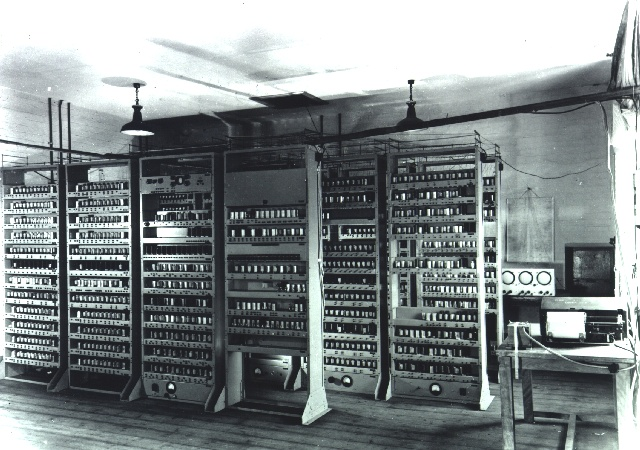
\includegraphics[width=0.95\linewidth]{EDSAC.jpg}
          \caption{\wikiEDSAC (Electronic Delay Storage Automatic Calculator) byl britský počítač z 
                   poloviny 20. století. Tento počítač, inspirovaný John Von Neumannovým dokumentem 
                   First Draft of a Report on the EDVAC, sestavil Maurice Wilkers a jeho tým na 
                   Univerzitě v Cambridgi v Anglii. EDSAC byl první v praxi využitý počítač 
                   pracující s uloženým programem. Kredit: Wikipedia, Root.cz}
          \label{MIT:fig_edsac}
        \end{figure}
        
        Na zpočátku pouze teoretickou práci M. V. Wilkese o několik let později navázali William 
        Renwick a \wikiWheeler, kteří v roce 1957 sestrojili první skutečný počítač založený na 
        mikroprogramovém procesoru. Vzhledem k tomu, že diodová matice navržená Wilkesem by byla 
        příliš rozměrná pro počítač s velkou instrukční sadou (diodami jsou zde samozřejmě myšleny 
        diskrétní elektronické součástky, i když se v roce 1957 již pomalu schylovalo k výrobě 
        prvních prototypů integrovaných obvodů), použili W. Renwick a D. Wheeler namísto diod 
        feritovou paměť, což bylo ve svém důsledku velmi zajímavé, protože se obsah této paměti dal 
        přeprogramovat a tím pádem bylo možné i měnit instrukční sadu počítače. První prototyp 
        tohoto stroje byl nazván \texttt{EDSAC 1½} a používal pro uložení mikroinstrukcí feritovou 
        paměť s maticí o velmi malých rozměrech 6×8 feritových jader – tento počítač ovšem 
        neobsahoval celou instrukční sadu. Finální podoba počítače z roku 1958, jež nesla název 
        \texttt{EDSAC 2}, měla již paměťovou matici o rozměrech 32×32 feritových jader, což již 
        umožnilo implementaci plnohodnotné instrukční sady za použití mikrokódů.
    
} % tikzset
%---------------------------------------------------------------------------------------------------
\printbibliography[title={Seznam literatury}, heading=subbibliography]
\addcontentsline{toc}{section}{Seznam literatury} 
%  % !TeX spellcheck = cs_CZ
{\tikzset{external/prefix={tikz/CES/}}
 \tikzset{external/figure name/.add={ch04_}{}}
%---------------------------------------------------------------------------------------------------
% file technology.tex
%---------------------------------------------------------------------------------------------------
%==============================Kapitola: Číslicové součástky a technologie=========================
\chapter{Číslicové součástky a technologie}
\minitoc

  \section{Rozdělení číslicových integrovaných obvodů}
    Logické integrované obvody zpracovávají nespojité signály, které nabývají jen konečného malého
    počtu úrovní. Naprostá většina dnes vyráběných logických IO využívá pouze dvou logických úrovní
    pracujících s dvojkovou číselnou soustavou. Jejich funkci a vzájemné spojování do soustav lze
    popsat pomocí Booleovy algebry (viz kap. \ref{CES:basic_bool_alg}) \cite[p.~8]{Musil2002}.
    
    Digitální IO se vyrábějí v technologii \emph{bipolární} (kap. \ref{CES:Bipolar_technology}) i
    \emph{unipolární} \ref{CES:Unipolar_technology} (především MOS). Základní kriteria, podle
    kterých posuzujeme kvalitu (vhodnost pro danou aplikaci) jednotlivých druhů (tříd) digitálních
    obvodů jsou:
    \begin{itemize}\addtolength{\itemsep}{-0.5\baselineskip}
      \item rychlost,
      \item příkon,
      \item odolnost proti rušení,
      \item široký rozsah pracovních teplot,
      \item nízké rušení generované vlastním obvodem (proudové špičky při změnách stavu),
      \item snadnost realizace složitějších logických funkcí,
      \item dosažitelná hodnota základních hradel a možnosti velké integrace,
      \item nízká cena.    
    \end{itemize}
    Tyto požadavky splňuje každá třída digitálních obvodů pouze částečně. Proto se ve výrobě
    udržuje několik různých tříd digitálních obvodů, z nichž každá má zdůrazněnou některou z výše
    uvedených vlastností tak, jak to odpovídá její fyzikální podstatě.
   
    \subsection{Vlastnosti logických hradel}
  
  \section{Bipolární digitální obvody}\label{CES:Bipolar_technology}
      V bipolární technologii jsou skupiny logických obvodů charakterizovány z hlediska režimu
      činnosti tranzistorů a tvoří dvě základní skupiny. Jsou to logické IO - s tranzistory
      pracujícími:
      \begin{itemize}
        \item v saturaci: tranzistor spínán z vypnutého stavu do saturace,
        \item v nesaturačním - aktivním režimu: tranzistor přepínán mezi stavem vypnutým (nebo
              slabě sepnutým) a aktivním (nesaturačním) módem.
      \end{itemize}
      V obou skupinách je přepínanou součástkou \emph{tranzistor NPN}. \emph{Komplementární
      tranzistor PNP} je využíván pouze jako zatěžovací prvek nebo jako proudový zdroj; pro tyto
      účely se rovněž využívá i rezistor.
      \begin{figure}[ht!]
        \centering
        \subfloat[Součtový člen]{\label{ces:fig_D_OR}
          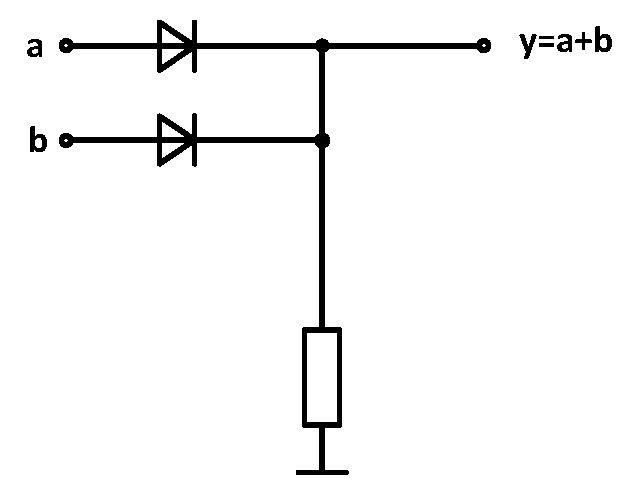
\includegraphics[width=0.3\linewidth]{diodovy_log_OR.pdf}}
        \subfloat[Součinový člen]{\label{ces:fig_D_AND}
          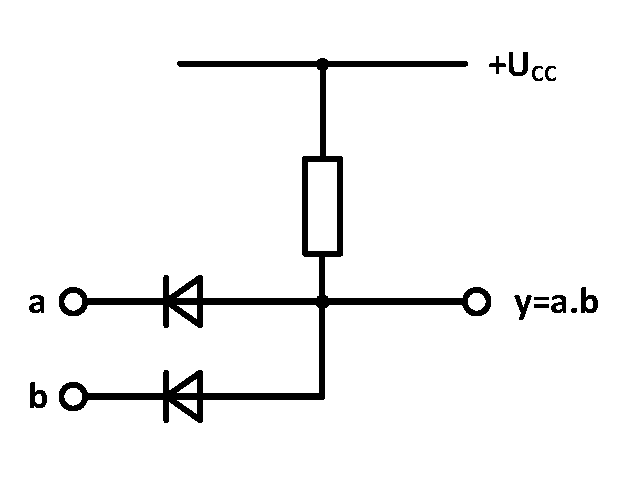
\includegraphics[width=0.3\linewidth]{diodovy_log_AND.pdf}}
        \caption{Diodová logika}
        \label{CES:fig_diodova_logika}
      \end{figure}
   \section{Unipolární digitální obvody}\label{CES:Unipolar_technology} 
  %-------------Přizpůsobení logických obvodů různých napěťových tříd-----------------------------
  % source: AN/Microchip/AN_3V_5V_Digital_Interfacing.pdf
  \newpage
  \section{Přizpůsobení logických obvodů různých napěťových tříd} %Digital Interfacing
    % When interfacing two devices that operate at different voltages, it is imperative to know the
    % output and input thresholds of both devices. Once these values are known, a technique can be
    % selected for interfacing the devices based on the other requirements of your application.
    % Table \ref{CES:tab_threshold} contains the output and input thresholds that will be used
    % throughout this document. When designing an interface, make sure to reference your
    % manufacturers data sheet for the actual threshold levels.
    Vyskytne-li se v číslicovém návrhu potřeba použít logická hradla z odlišných napěťových tříd,
    budeme postaveni před problém jejich vzájemného propojení zachovávající jejich funkčnost. Pro
    správnou volbu vhodného napěťového přizpůsobení logických hradel z různých rodin, je nutné znát
    nejen jejich rozhodovací napětí, ale také následující parametry, které jsou uvedeny v tabulce
    \ref{CES:tab_threshold} \cite[p.~22]{DS41285A}:
    
    \begin{itemize}\addtolength{\itemsep}{-0.5\baselineskip}
      \item maximální úroveň logické '0' na vstupu hradla - $\mathbf{V_{IL_{max}}}$
      \item minimální úroveň logické '1' na vstupu hradla - $\mathbf{V_{IH_{min}}}$
      \item maximální úroveň logické '0' na výstupu hradla - $\mathbf{V_{OL_{max}}}$
      \item minimální úroveň logické '1' na výstupu hradla - $\mathbf{V_{OH_{min}}}$
    \end{itemize}
    
    \begin{table*}
      \centering
      \begin{tabular}{|>{\columncolor{Tan}}l||c|c|c|c|}
        \hline
        \rowcolor{CornflowerBlue}{ }    & {$\mathbf{V_{OH_{min}}}$} & {$\mathbf{V_{OL_{max}}}$} & %
                                          {$\mathbf{V_{IH_{min}}}$} & {$\mathbf{V_{IL_{max}}}$} \\
        \hline
        \hline
        \texttt{5V TTL}                       
                    & 2.4V            & 0.5V       & 2.0V              & 0.8             \\
        \hline
        \texttt{3.3V LVTTL}          
                    & 2.4V            & 0.4V       & 2.0V              & 0.8             \\
        \hline
                    & 4.7V            & 0.5V       & 3.5V              & 1.5V            \\
        \multirow{-2}*{\texttt{5V CMOS}}      
                    & ($V_{CC}$-0.3V) &            & (0.7x$V_{CC}$)    & (0.3x$V_{CC}$)  \\
        \hline
                    
                    & 3.0V            & 0.5V       & 2.3V              & 1.0V            \\
        \multirow{-2}*{\texttt{3.3V LVCMOS}} 
                    & ($V_{CC}$-0.3V) &            & (0.7x$V_{CC}$)    & (0.3x$V_{CC}$)  \\
        \hline 
      \end{tabular}
      \caption{Rozhodovací úrovně napěťových tříd: \texttt{5V TTL}, \texttt{3.3V LVTTL}, 
                                                   \texttt{5V CMOS}, \texttt{3.3V
      LVCMOS}}\label{CES:tab_threshold}
    \end{table*}
    Úroveň logické nuly a jedničky na výstupu určuje konstrukce koncové části digitálního obvodu.
    Nejčastější provedení jsou na obr. \ref{ces:fig_digit_out_common}. Jsou-li různé digitální
    obvody připojeny na společnou sběrnici, může dojít k situaci, kdy některý z výstupních vývodů
    bude buzen vyšším napětím než je napájecí napětí příslušného obvodu. I v tomto případě výstupní
    část digitálního obvodu rozhoduje o výsledném chování. Shrňme základní vlastnosti technologií
    číslicových obvodů uvedených na obr. \ref{ces:fig_digit_out_common}:
    \begin{itemize}
      \item Bipolární koncový stupeň nedovoluje plný rozkmit výstupního signálu. Je-li obvod
            napájen \SI{5}{\volt}, je výstup při úrovni H limitován na $V_{CC}-2\times V_{BE}$(cca
            3.6V). To je hodnota, která na rozhraní \SI{3}{\volt} systému nezpůsobuje příliš velký
            napěťový rozdíl, a tedy proudu, tekoucímu z napájecího zdroje \SI{5}{\volt} systému do
            zdroje \SI{3}{\volt} systému.
      \item Výstupní napětí typické \texttt{CMOS} součástky se prakticky pohybuje v rozsahu
            \texttt{GND} - \texttt{VCC}.
      \item Některé součástky mají výstup typu \emph{open kolektor - OC} resp. \emph{open drain -
            OD}, tj. neexistuje vnitřní obvod, jenž by uvedl výstup do stavu H. K tomu je zapotřebí
            \emph{pull-up} rezistoru, který připojí výstup k napětí, které může být i vyšší než je
            napájecí - \texttt{VCC}. Očividně, tento způsob umožňuje relativně snadné rozhraní, ale
            pro dosažení vyšších rychlostí je nutné volit relativně malý odpor, což zvyšuje
            spotřebu.
      \item U \texttt{NMOS} stupně je podobně jako u bipolárního stupně výstupní napětí logické
            úrovně H omezeno úbytkem na kanálu horní NMOS tranzistoru na $V_{CC} - V_{TH}\simeq
            \SI{3.5}{\volt}$. Obvykle je tedy možné přímé řízení 3V systému.
    \end{itemize}

    \begin{figure}[ht!]
         \centering
         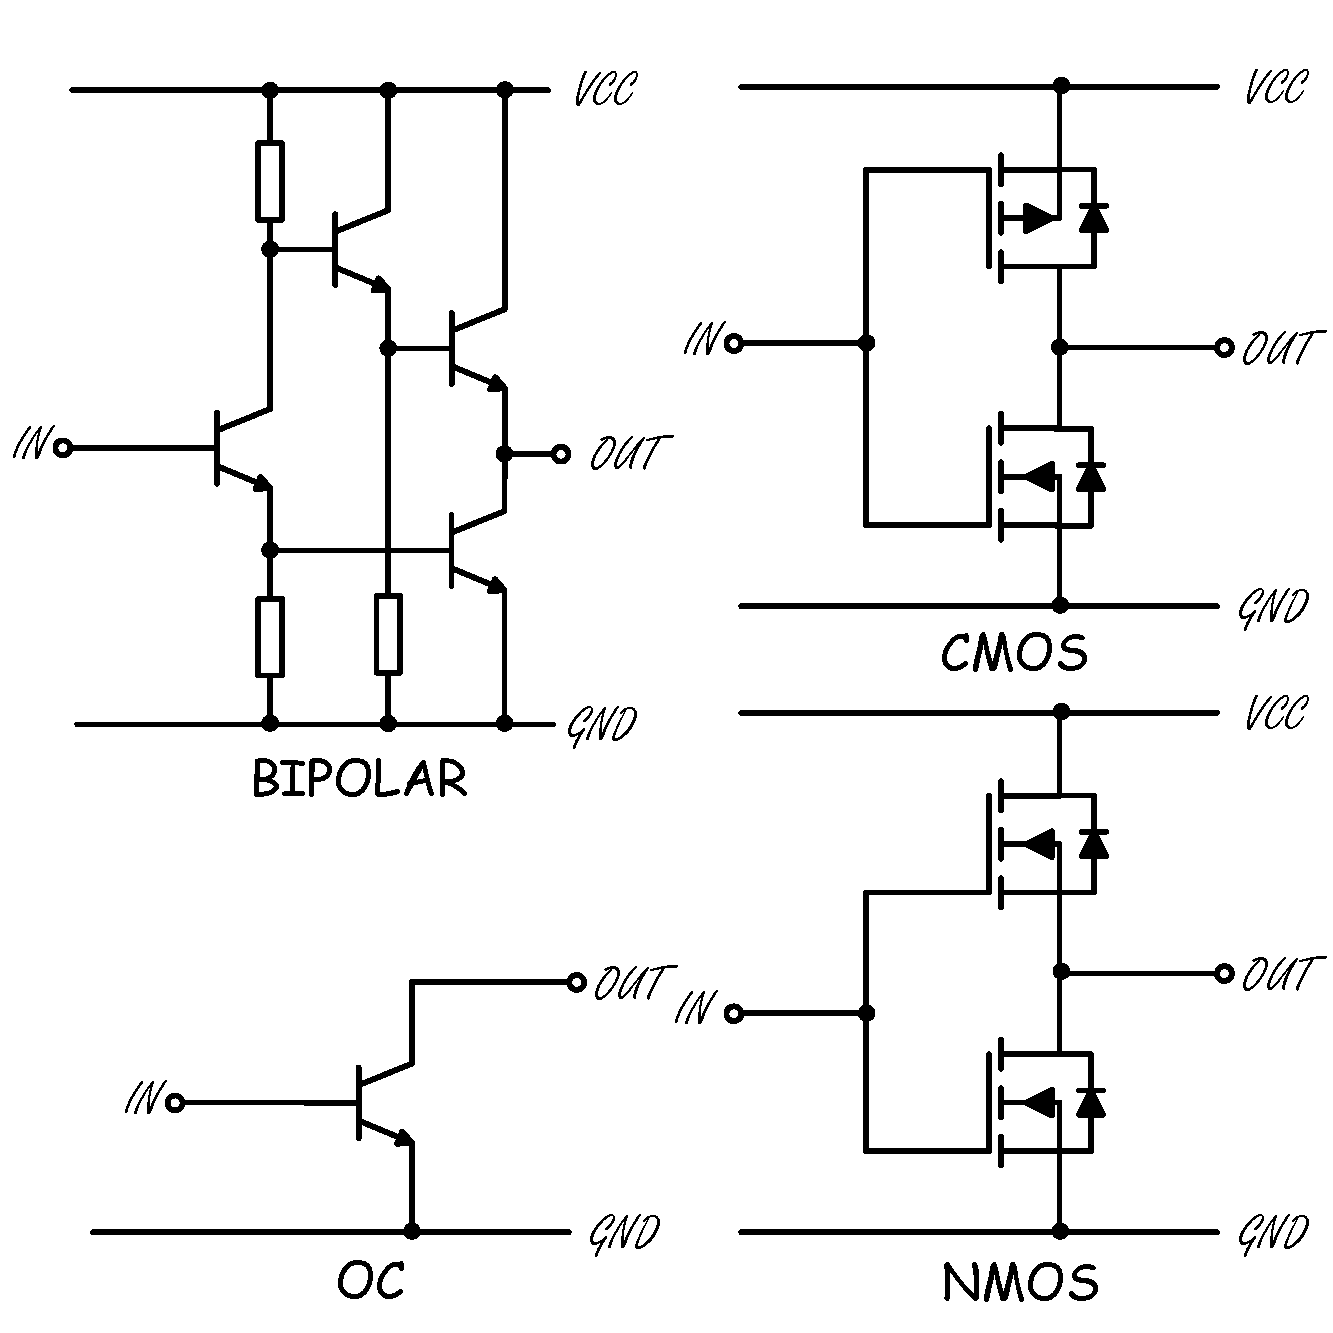
\includegraphics[width=0.7\linewidth]{digit_cir_output_common.pdf}
         \caption[Koncové stupně digitálních obvodů]
                 {Koncové stupně bipolárních, CMOS, NMOS obvodů a obvodů s otevřeným kolektorem 
                  \cite[p.~2]{AN240}}
         \label{ces:fig_digit_out_common}
    \end{figure}   
    
    % --------  Přizpůsobení: 3.3V -> 5V --------------------------- 
    \subsection{3.3V $\rightarrow$ 5V} %3.3V to 5V
      % The simplest and most desired way to connect a 3.3V output to a 5V input is by a direct
      % connection.  This can be done only if the following 2 requirements are met:
      Nejjednodušším a nejvíce žádoucím způsobem je přímé připojení 3.3V výstupu k 5V vstupu, což
      lze provést pouze v případě, že jsou splněny následující požadavky:
        \begin{itemize}\addtolength{\itemsep}{-0.5\baselineskip}
          \item $V_{OH}(3.3V)>V_{IH}(5V)$,
          \item $V_{OL}(3.3V)<V_{IL}(5V)$.
        \end{itemize}
      Hodnoty prahových napětí logické nuly a jedničky v předchozí tabulce \ref{CES:tab_threshold}
      dokládají, že v případě logiky \texttt{3.3V LVCMOS} a \texttt{5V TTL} je možné použít přímého
      připojení. 
      % An example of when this technique can  be used is interfacing a 3.3V LVCMOS output to a 5V
      % TTL input. From the values given in Table 4-1, it can clearly be  seen that both of these
      % requirements are met.

      % 3.3V LVCMOS VOH of 3.0 volts is greater than 5V TTL VIH of 2.0 volts and 3.3V LVCMOS VOL
      % of 0.5 volts is less than 5V TTL VIL of 0.8 volts.

      Pokud oba tyto požadavky nejsou splněny, je třeba použít na rozhraní obou logik
      přizpůsobovací obvody, popsané v následujících textu. 
      % When both of these requirements are  not met, some additional circuitry will be needed to
      % interface the two parts.

      \subsubsection{MOSFET Translator}
        \begin{figure}[ht!]
           \centering
           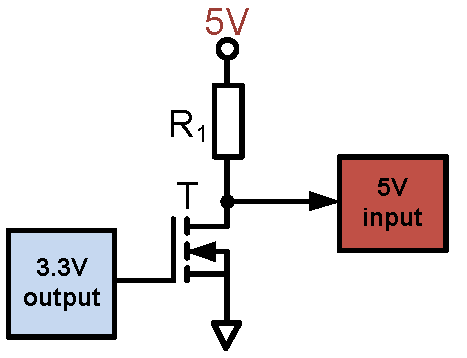
\includegraphics[scale=0.5]{level_shifting_MOSFET.pdf}
           \caption{3.3V $\rightarrow$ 5V: N-MOSFET}
           \label{CES:fig_shifting_MOSFET}
           \vspace*{-1\baselineskip}
        \end{figure}
        % In order to drive any 5V input that has a higher VIH than the VOH of a 3.3V CMOS part,
        % some additional circuitry is needed. A low-cost two component solution is shown in Figure
        % 6-1. When selecting the value for R1, there are two parameters that need to be considered;
        % the switching speed of the input and the current consumption through R1.
        Levné a jednoduché řešení problému vzájem\-ného přizpůsobení logických obvodů odliš\-ných
        napěťových tříd, pro které platí $V_{OH}(3.3V)<V_{IH}(5V)$ nabízí použití MOSFETu s
        prahovým napětím $$V_{GS_{th_{max}}}<V_{OH_{min}}.$$ Při výběru hodnoty $R_1$ je třeba vzít
        v úvahu:
        \begin{itemize}\addtolength{\itemsep}{-0.5\baselineskip}
          \item spínací rychlost vstupu,
          \item zvýšení spotřeby díky proudu přes rezistor $R_1$.
        \end{itemize}

        Při změně logické úrovně $'0'\rightarrow'1'$ na vstupu 5V logiky je nutné počítat se
        zpožděním, které je dáno časovou konstantu RC článku, tvořeného rezistorem $R_1$ a celkovou
        kapacitou na vstupu hradla. Důsledkem je tedy určitá minimální spínací perioda: 
        % When switching the input from a ‘0’ to a ‘1’, you will have to account for the time the
        % input takes to rise because of the RC time constant formed by R1, and the input
        % capacitance of the 5V input plus any stray capacitance on the board. The speed at which
        % you can switch the input is given by the following:
        $$T_{SW_{min}} = 3 \cdot R_1 \cdot C_{IN},$$ která je vyšší, čím nižší spotřeby se návrhář
        snaží dosáhnout ($R_1\uparrow$). Zpoždění při spínání $'1'\rightarrow'0'$ má příznivější
        hodnotu, neboť $R_{dsON}\ll R_1$.

        % Since the input and stray capacitance of the board are fixed, the only way to speed up
        % the switching of the input is to lower the resistance of R1. The trade-off of lowering
        % the resistance of R1 to get faster switching times is the increase in current draw when
        % the 5V input remains low. The switching to a ‘0’ will typically be much faster than
        % switching to a ‘1’ because the ON resistance of the N-channel MOSFET will be much smaller
        % than R1. Also, when selecting the N-channel FET, select a FET that has a lower VGS
        % threshold voltage than the VOH of 3.3V output.

      \subsubsection{Diodový Offset}
        Hodnoty vstupního prahového napětí \texttt{5V CMOS} a výstupní prahová napětí pro
        \texttt{3.3V LVTTL} a \texttt{LVCMOS} jsou uvedeny v tabulce \ref{CES:tab_diode_offset}
        % The inputs voltage thresholds for 5V CMOS and the output drive voltage for 3.3V LVTTL and
        % LVCMOS are listed in Table 7-1.
        \begin{table*}[t]
          \centering
          \begin{tabular}{|>{\columncolor{Tan}}l|c|c|c|}
            \hline
              \cellcolor{CornflowerBlue}                                   
                & \cellcolor{CornflowerBlue}\textbf{5V CMOS}       & 
              \cellcolor{CornflowerBlue} \textbf{3.3V LVTTL}               
                & \cellcolor{CornflowerBlue} \textbf{3.3V LVCMOS}  \\
              \multirow{-2}*{\cellcolor{CornflowerBlue}\texttt{Threshold}} 
                & \cellcolor{CornflowerBlue} IN 
                & \cellcolor{CornflowerBlue} OUT
                & \cellcolor{CornflowerBlue} OUT                   \\
            \hline\hline
               \texttt{High}                                               
                & $>3.5V$  & $>2.4V$ & $>3.0V$                     \\
               \texttt{Low}                                         
                & $<1.5V$  & $<0.4V$ & $<0.5V$                     \\
            \hline          
          \end{tabular}
          \caption{Přehled vstupní a výstupních prahový napětí různých logik, chceme-li ke vstupu
          \texttt{5V CMOS} připojit \texttt{3.3V LVTTL} nebo \texttt{3.3V LVCMOS.\cite{AN240}}}
          \label{CES:tab_diode_offset}
        \end{table*}

        \begin{figure}[ht!]
            \centering
            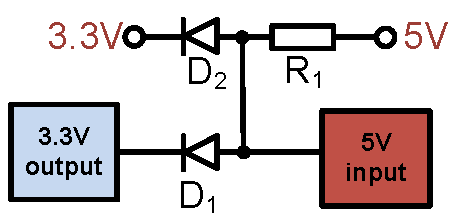
\includegraphics[scale=0.5]{level_shifting_diode_offset.pdf}
            \caption{3.3V $\rightarrow$ 5V: Diodový offset}
            \label{CES:fig_shifting_D_offset}
        \end{figure}

        Všimněme si, že obě prahová napětí vstupu \texttt{5V CMOS} logiky jsou o volt vyšší než u
        výstupu 3.3V logiky. Zapotřebí je tedy obvod, který zvyšuje vysokou a nízkou úroveň
        prahového napětí.
        % Note that both the high and low threshold input voltages for the 5V CMOS inputs are about
        % a volt higher than the 3.3V outputs. So, even if the output from the 3.3V system could be
        % offset, there would be little or no margin for noise or component tolerance. What is
        % needed is a circuit that offsets the outputs and increases the difference between the
        % high and low output voltages.

        Pokud bychom vytvořili posunutí o alespoň o 0.7V pro obě úrovně prahového napětí, dosáhli
        bychom vzájemného přizpůsobení. Obvod na obr. \ref{CES:fig_shifting_D_offset}, posuneme
        hodnotu nízké úrovně výstupního prahového napětí o úbytek v propustném směru diody $D_1$
        (typicky 0.7V), na 1.1V až 1.2V. Úroveň vysokého prahového napětí se nastavuje pomocí
        pull-up rezistoru a diody $D_2$ vázané na 3.3V napájení. Výstupní napětí je tedy také
        posunuto přibližně 0,7V nad 3,3V napájení, tj. na 4,0 až 4.1V, což je vysoko nad 3,5V
        prahem vstupu 5V CMOS logiky.

        % When output voltage specifications are determined, it is done assuming that the output is
        % driving a load between the output and ground for the high output, and a load between 3.3V
        % and the output for the low output. If the load for the high threshold is actually between
        % the output and 3.3V, then the output voltage is actually much higher as the load resistor
        % is the mechanism that is pulling the output up, instead of the output transistor.

        % If we create a diode offset circuit (see Figure 7-1), the output low voltage is increased
        % by the forward voltage of the diode D1, typically 0.7V, creating a low voltage at the 5V
        % CMOS input of 1.1V to 1.2V. This is well within the low threshold input voltage for the
        % 5V CMOS input. The output high voltage is set by the pull-up resistor and diode D2, tied
        % to the 3.3V supply. This puts the output high voltage at approximately 0.7V above the
        % 3.3V supply, or 4.0 to 4.1V, which is well above the 3.5V threshold for the 5V CMOS input
        \vskip2mm
        \begin{note}
          Aby obvod fungoval správně, musí být pull-up rezistor podstatně menší než vstupní odpor
          5V CMOS logiky, aby se zabránilo snížení výstupního napětí díky efektu vstupního
          odporového děliče a také musí být dostatečně velký, aby proud tekoucí do 3.3V napájení a
          výstupu hradla byl v mezích specifikace. 
          % For the circuit to work properly, the pull-up resistor must be significantly smaller
          % than the input resistance of the 5V CMOS input, to prevent a reduction in the output
          % voltage due to a resistor divider effect at the input. The pull-up resistor must also
          % be large enough to keep the output current loading on the 3.3V output within the
          % specification of the device.
        \end{note}

      \subsubsection{Komparátor}
        Základní funkce komparátoru je následující:        
        % The basic operation of the comparator is as follows:
        \begin{itemize}\addtolength{\itemsep}{-0.5\baselineskip}
          \item napětí na invertující (-) vstupu je větší než na neinvertujícím vstupu (+), výstup
                komparátoru se nastaví do nízké úrovně, 
                % When the voltage at the inverting (-) input is greater than that at the
                % non-inverting (+) input, the output of the comparator swings to Vss.
          \item je-li napětí na neinvertujícím vstupu (+) větší než na invertujícím vstupu (-),
                výstup komparátoru se nastaví do vysoké úrovně. %When the voltage at the
                % non-inverting (+) input is greater than that at the non-inverting (-)
                % input, the output of the comparator is in a high state.
        \end{itemize}

        \begin{figure}[ht!]
            \centering\vspace*{+1\baselineskip}
            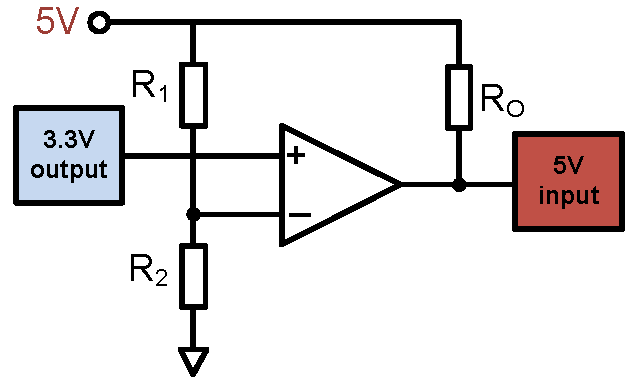
\includegraphics[scale=0.5]{level_shifting_COMP.pdf}
            \caption{3.3V $\rightarrow$ 5V: Komparátor; $R_1 = 1,8 k\Omega, R_2 = 1 k\Omega$}
            \label{CES:fig_shifting_COMP}           
        \end{figure}

        \textbf{Výpočet hodnoty odporu $R_1$ a $R_2$:}\newline
          Poměr R1 a R2 je závislý na napětí logické nuly a jedničky na výstupu hradla 3.3V logiky.
          Invertující vstup by měl být nastaven do poloviny mezi prahovými hladinami $V_{OL}$ a
          $V_{OH}$. Pro \texttt{LVCMOS} je toto napětí rovno $$1.75V = \frac{3V+0.5V}{2}.$$
          Budeme-li volit velikost $R_2$, pak hodnotu odporu $R_1$ snadno dopočítáme dle
          následující rovnice: $$R_1=R_2\left(\frac{5V}{1.75V}-1\right).$$ 
          % The ratio of R1  and R2  depends on the logic levels of the input signal. The inverting
          % input should be set to a voltage halfway between VOL and VOH for the 3.3V output. For
          % an LVCMOS output, this voltage is: $$1.75V = \frac{3V+0.5V}{2}.$$ Given that R1 and R2
          % are related by the logic levels:
          % $$R_1=R_2\left(\frac{5V}{1.75V}-1\right)$$ assuming a value of 1K for R2, R1 is 1.8K.

    % --------  Přizpůsobení: 5V -> 3.3V ---------------------------
    \subsection{5V $\rightarrow$ 3.3V} %5V to 3.3V
      \subsubsection{Přímé propojení}
        \begin{figure}[ht!]
            \centering
            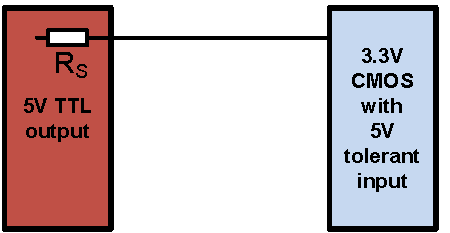
\includegraphics[scale=0.6]{direct_connect.pdf}
            \caption{5V $\rightarrow$ 3,3V: Přímé propojení}
            \label{CES:fig_dir_connect}
        \end{figure}

        Hradla napěťové třídy 5V mají výstupy s typickými prahovými hodnotami $V_{OH} = 4,7 V$,
        $V_{OL} = 0,4 V$ zatímco hradla 3.3V LVCMOS mají vstupy s prahovými hodnotami $V_{IH} =
        0,7\times V_{DD} $, $V_{IL} = 0,2\times V_{DD}$. Je-li tedy na 5V výstupu logická nula,
        bude také správně interpretována 3V vstupem, neboť platí $V_{OL} = 0,4 < V_{IL} = 0,8$. Ani
        v případě logické jedničky nevzniká žádný konflikt, neboť $V_{OH} = 4,7 > V_{IH} = 2,1$.
        Pokud je tedy 3V vstup 5V tolerantní, je možné přímé propojení, v opačném případě je třeba
        použít některou z následujících technik.
        % 5V outputs have a typical VOH of 4.7 volts and a VOL of 0.4 volts and a 3.3V LVCMOS input
        % will have a typical VIH of 0.7 x VDD and a VIL of 0.2 x VDD. When the 5V output is
        % driving low, there are no problems because the 0.4 volt output is less than in the input
        % threshold of 0.8 volts. When the 5V output is high, the VOH of 4.7 volts is greater than
        % 2.1 volt VIH, therefore, we can directly connect the 2 pins with no conflicts if the 3.3V
        % CMOS input is 5 volt tolerant. If the 3.3V CMOS input is not 5 volt tolerant, then there
        % will be an issue because the maximum volt specification of the input will be exceeded.

      \subsubsection{Diodový omezovač} %Diode Clamp
        Některé digitální obvody mají své vstupy chráněny vnitřními omezovacími diodami tzv.
        \texttt{diode clamp} (obr. \ref{CES:fig_int_clamp_D}). Proteče-li těmito diodami větší proud
        než udávají katalogové hodnoty, může dojít k poškození vstupu, nebo v lepším případě k
        efektu \texttt{latching-up}. Typický 5V výstup má kolem $10 \Omega$, proto chceme-li využít
        těchto diod, musíme přidat sériový odpor, jenž limituje velikost propustného proudu.
        Nepříjemným důsledkem je ovšem vzniklý RC článek se vstupní kapacitou hradla $C_L$, který
        snižuje rychlost. Není-li vstup takto chráněn je možné jej doplnit externí diodou dle obr.
        \ref{CES:fig_ext_clamp_D}.
        % Many manufacturers protect their I/O pins from exceeding the maximum allowable voltage
        % specification by using clamping diodes. These clamping diodes keep the pin from going
        % more than a diode drop below Vss and a diode drop above VDD. To use the clamping diode to
        % protect the input, you still need to look at the current through the clamping diode. The
        % current through the clamp diodes should be kept small (in the micro amp range). If the
        % current through the clamping diodes gets too large, then you risk the part latching up.
        % Since the source resistance of a 5V output is typically around 10 ohms, an additional
        % series resistor is still needed to limit the current through the clamping diode as shown
        % Figure 10-1. The consequence of using the series resistor is it will reduce the speed at
        % which we can switch the input because the RC time constant formed the capacitance of the
        % pin (CL).
       \begin{figure}[ht!]
         \centering
         \begin{tabular}{c}
           \subfloat[Vnitřními omezovací diody]{\label{CES:fig_int_clamp_D}
             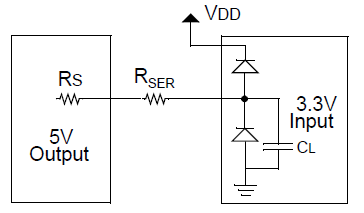
\includegraphics[width=0.3\textwidth]{CES_clamp_diodes_input.png}}        \\
           \subfloat[Externí omezovací dioda]{\label{CES:fig_ext_clamp_D}     
             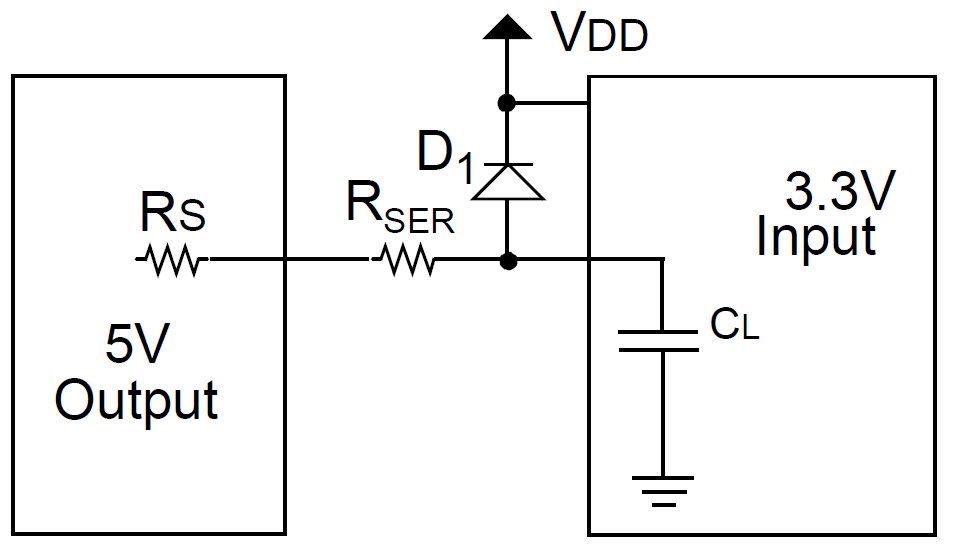
\includegraphics[width=0.3\textwidth]{CES_ext_clamp_diodes_input.png}}
         \end{tabular}  
         \caption{5V $\rightarrow$ 3,3V: Použití omezovacích diod pro ochranu vstupu integrovaného
                  obvodu}
         \label{CES:fig_clamp_diodes}
       \end{figure} 
        % One problem with using a diode clamp is that it injects current onto the 3.3V power
        % supply. In designs with a high current 5V outputs, and lightly loaded 3.3V power supply
        % rails, this injected current can float the 3.3V supply voltage above 3.3V. To prevent
        % this problem, a transistor can be substituted which routes the excess output drive
        % current to ground instead of the 3.3V supply.
          
        Dalším problémem je proud, injektovaný z 5V výstupu skrz omezovovací diodu do 3.3V
        napájení. Tento proud může způsobit zvýšení napájecího napětí 3.3V obvodů, což může vést k
        jejich zničení. Proto lze s výhodou použít PNP tranzistor zapojený dle obr.
        \ref{CES:fig_bjt_clamp}.
        
        \begin{figure}[ht!]
          \centering
          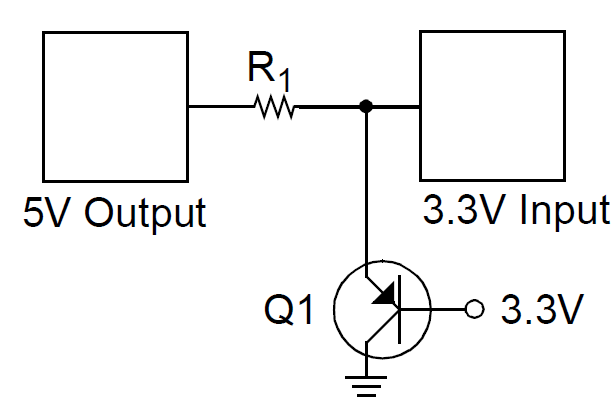
\includegraphics[scale=0.5]{CES_ext_clamp_bjt_input.png}
          \caption{5V $\rightarrow$ 3,3V: Active clamp - Přechod báze-emitor funguje jako omezovací
                   dioda, ovšem s tím rozdílem, že jen malé procento celkového proudu z 5V výstupu
                   teče do 3.3V napájení. Převážná část teče kolektorem do země. Poměr bázového a
                   kolektorového proudu je určen proudovým zesílením tranzistoru, které je typicky
                  10 až 400}
          \label{CES:fig_bjt_clamp}
        \end{figure}              
       
      \subsubsection{Napěťový dělič} %Resistor divider
        A simple resistor divider can be used to reduce the output of a 5V device to levels
        appropriate for a 3.3V device input. An equivalent circuit of this interface is shown in
        Figure \ref{CES:fig_res_divider}.
        \begin{figure}[ht!]
          \centering
          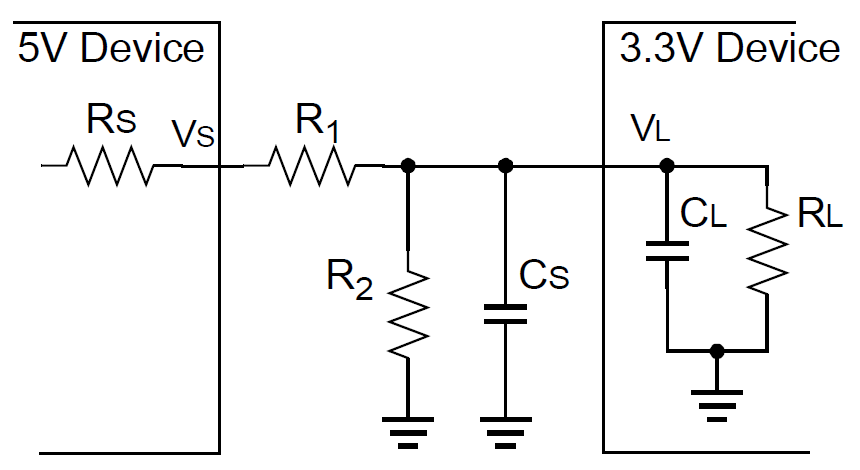
\includegraphics[scale=0.4]{CES_ext_res_divider.png}
          \caption{5V $\rightarrow$ 3,3V: napěťový děliš}
          \label{CES:fig_res_divider}
        \end{figure}
        Typically, the source resistance, $R_S$, is very small (less than 10 ohms) so its affect on
        $R_1$ will be negligible provided that $R_1$ is chosen to be much larger than $R_S$. At the
        receive end, the load resistance, $R_L$, is very large (greater than 500 k ohms) so its
        affect on $R_2$ will be negligible provided that $R_2$ is chosen to be much less than
        $R_L$.
        
        There is a trade-off between power dissipation and transition times. To keep the power
        requirements of the interface circuit at a minimum, the series resistance of $R_1$ and
        $R_2$ should be as large as possible. However, the load capacitance, which is the
        combination of the stray capacitance, $C_S$, and the 3.3V device input capacitance, $C_L$,
        can adversely affect the rise and fall times of the input signal. Rise and fall times can
        be unacceptably long if $R_1$ and $R_2$ are too large.
        
        Neglecting the affects of $R_S$ and $R_L$, the formula for determining the values for $R_1$
        and $R_2$ is given by Equation \ref{CES:eq_res_divider}.
        \begin{align}\label{CES:eq_res_divider}
          \frac{V_S}{R_1+R_2} &= \frac{V_L}{R_2}           \nonumber \\
                          R_1 &= \frac{(V_S-V_L)}{V_L}R_2  \nonumber \\
                          R_1 &= 0,515\cdot R_2
        \end{align}      
        The formula for determining the rise and fall times is given in Equation
        \ref{CES:eq_res_divider_time}. For circuit analysis, the Thevenin equivalent is used to
        determine the applied voltage, $V_A$, and the series resistance, $R$.
        The Thevenin equivalent is defined as the open circuit voltage divided by the short circuit
        current. The Thevenin equivalent, $R$, is determined to be $0.66\cdot R_1$ and the Thevenin
        equivalent, $V_A$, is determined to be $0.66\cdot V_S$ for the circuit shown in  Figure
        \ref{CES:fig_res_divider} according to the limitations imposed by Equation
        \ref{CES:eq_res_divider_time}.
        \begin{equation}\label{CES:eq_res_divider_time}
          t = - R\cdot C \cdot \ln\left(\frac{V_F-V_A}{V_I-V_A}\right)
        \end{equation}  
        kde $t$ = Rise or Fall time, $R = 0.66\cdot R_1$, $C = C_S+C_L$, $V_I$ = Initial voltage on
        $C$ ($V_L$), $V_F$ = Final voltage on $C$ ($V_L$), $V_A$ = Applied voltage ($0.66\cdot V_S$). 
        \begin{example} As an example, suppose the following conditions exist:
          \begin{itemize}\addtolength{\itemsep}{-0.5\baselineskip}
            \item Stray capacitance = 30 pF,
            \item Load capacitance = 5 pF,
            \item Maximum rise time from 0.3V to 3V ≤ 1 μS
            \item Applied source voltage Vs = 5V
          \end{itemize}
          Solve Equation \ref{CES:eq_res_divider_time} for $R$:  
          \begin{equation*}
            R = - \dfrac{t}{C\cdot\ln\dfrac{V_F-V_A}{V_I-V_A}}
          \end{equation*}   
          Substitute values:
          \begin{equation*}
            R = - \dfrac{10\cdot10^{-7}}{35\cdot10^{-12}\cdot
                  \ln\dfrac{3-0.66\cdot5}{0.3-0.66\cdot5}}
          \end{equation*}               
          Thevenin equivalent maximum R: $$R = 12408$$
          Solve for maximum $R_1$ and $R_2$:
          \begin{alignat}{3}
            & R_1 &&= 0.66\cdot R  \qquad &&R_2 = \frac{R_1}{0.515}  \\
            & R_1 &&= 8190         \qquad &&R_2 = 15902 
          \end{alignat}          
        \end{example} 
                   
      \subsubsection{Level translator} %Level translator
        While level translation can be done discretely, it is often preferred to use an integrated
        solution. Level translators are available in a wide range of capabilities. There are
        unidirectional and bidirectional configurations, different voltage translations and
        different speeds, all giving the user the ability to select the best solution. 
        \begin{figure}[ht!]
          \centering
          \begin{tabular}{c}
            \subfloat[SPI sběrnice]{\label{CES:fig_level_translator1}
              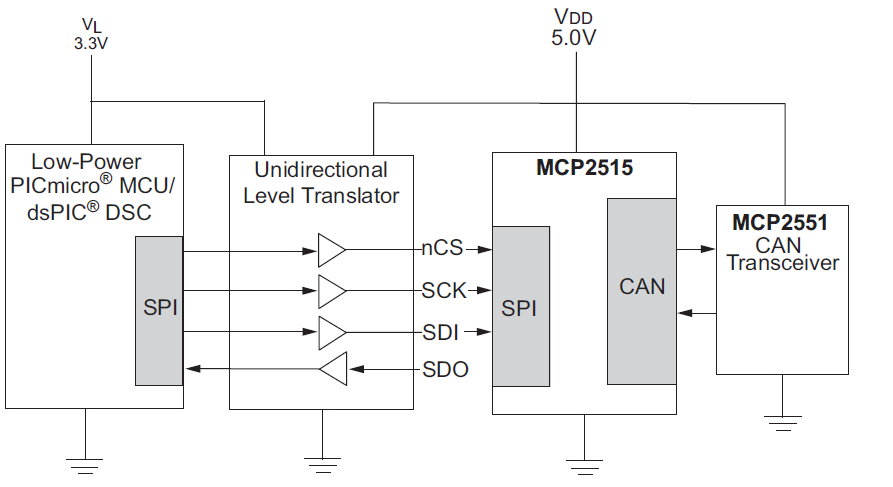
\includegraphics[width=0.9\linewidth]{CES_ext_level_translator1.png}}           \\
            \subfloat[I2C sběrnice]{\label{CES:fig_level_translator2}
              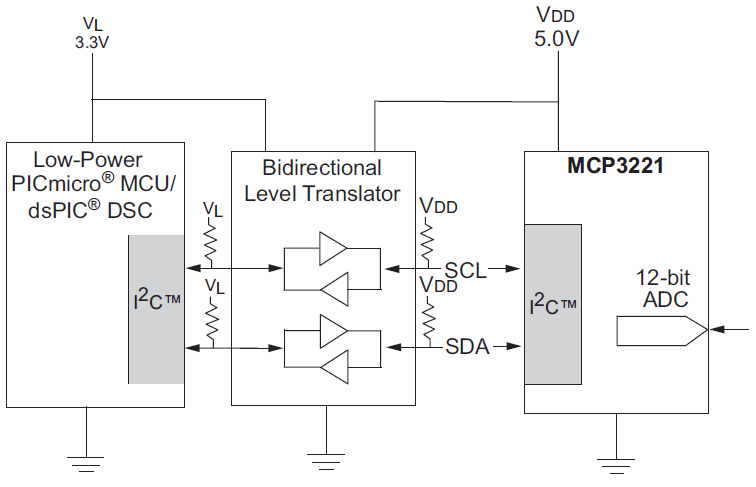
\includegraphics[width=0.9\linewidth]{CES_ext_level_translator2.png}}
          \end{tabular}  
          \caption{5V $\rightarrow$ 3,3V: Board-level communication between devices (e.g., MCU to
                   peripheral) is most often done by either SPI or I2C. For SPI, it may be
                   appropriate to use a unidirectional level translator and for I2C, it is necessary
                   to use a bidirectional solution.}
          \label{CES:fig_level_translator}
        \end{figure}           
      
} % tikzset
%---------------------------------------------------------------------------------------------------
\printbibliography[title={Seznam literatury}, heading=subbibliography]
\addcontentsline{toc}{section}{Seznam literatury} 
  % !TeX spellcheck = cs_CZ
{\tikzset{external/prefix={tikz/CES/}}
 \tikzset{external/figure name/.add={ch03_}{}}
%---------------------------------------------------------------------------------------------------
% file Basic_MCU_Arch.tex
%---------------------------------------------------------------------------------------------------
\lstset{ %
  language={[x86masm]Assembler},         % choose the language of the code
  inputencoding=latin1,
  extendedchars=true,
  showspaces=false,                      % show spaces everywhere adding particluar undescores, it  
                                         % overrides 
                                         % “showstringspaces”
  showstringspaces=false,                % underline spaces within strings only
  basicstyle=\footnotesize\ttfamily,     % the size of the fonts that are used for the code
%  backgroundcolor=\color{White},        % choose the background color. You must add  
                                         % \usepackage{color}
  breaklines=true,                       % sets automatic line breaking
  breakatwhitespace=true,                % sets if automatic breaks should only happen at whitespace
  showspaces=false,                      % show spaces adding particular underscores
  showstringspaces=true,                 % underline spaces within strings
  showtabs=true,                         % show tabs within strings adding particular underscores
  frame=none,                            % adds a frame around the code - none, single
  tabsize=2,                             % sets default tabsize to 2 spaces
  captionpos=b,                          % sets the caption-position to bottom
  numbers=left,                          % where to put the line-numbers -none, left, right
  numberstyle=\tiny\color{lstnumcolor},  % the size of the fonts that are used for the line-numbers
  numbersep=5pt,                         % how far te line-number are from the code
  stepnumber=1,                          % the step between two line-numbers. If it's 1 each line
                                         % will be numbered
  xleftmargin=3em,                       % adjust left margin
  commentstyle=\color{help}\textit,      % comment style
  keywordstyle=\color{keyword}\textbf,   % keyword style
  morekeywords={ADDC, ASHR, SUBB,CLR,    % if you want to add more keywords to the set
    MAC,  MULS, DIVS, BSET, BCLR, BCPL, 
    BAND, BOR,  BXOR, BCMP, TRL,  EX,  BMOV,
    JCC,  BCC,  DJNZ, RETI, JSR,  CSP, LDR},
  literate= %
    {á}{{\'a}}1  {é}{{\'e}}1     {í}{{\'i}}1   {ó}{{\'o}}1   {ú}{{\'u}}1
    {Á}{{\'A}}1  {É}{{\'E}}1     {Í}{{\'I}}1   {Ó}{{\'O}}1   {Ú}{{\'U}}1
    {à}{{\`a}}1  {è}{{\`e}}1     {ì}{{\`i}}1   {ò}{{\`o}}1   {ù}{{\`u}}1
    {À}{{\`A}}1  {È}{{\'E}}1     {Ì}{{\`I}}1   {Ò}{{\`O}}1   {Ù}{{\`U}}1
    {ä}{{\"a}}1  {ë}{{\"e}}1     {ï}{{\"i}}1   {ö}{{\"o}}1   {ü}{{\"u}}1
    {Ä}{{\"A}}1  {Ë}{{\"E}}1     {Ï}{{\"I}}1   {Ö}{{\"O}}1   {Ü}{{\"U}}1
    {â}{{\^a}}1  {ê}{{\^e}}1     {î}{{\^i}}1   {ô}{{\^o}}1   {û}{{\^u}}1
    {Â}{{\^A}}1  {Ê}{{\^E}}1     {Î}{{\^I}}1   {Ô}{{\^O}}1   {Û}{{\^U}}1
    {œ}{{\oe}}1  {Œ}{{\OE}}1     {æ}{{\ae}}1   {Æ}{{\AE}}1   {ß}{{\ss}}1
    {ç}{{\c c}}1 {Ç}{{\c C}}1    {ø}{{\o}}1    {å}{{\r a}}1  {Å}{{\r A}}1
    {€}{{\EUR}}1 {£}{{\pounds}}1 {ř}{{\v{r}}}1 {ž}{{\v{z}}}1 {č}{{\v{c}}}1
    {ě}{{\v{e}}}1
}
%====================Kapitola: Základy mikroprocesorové techniky====================================
%\setchaptertoc
\chapter{Základy mikroprocesorové techniky}
\minitoc

  Cílem této kapitoly není výklad, zaměřený pouze na jeden typ obvodu, nýbrž zobecnění základních 
  vlastnosti mikropočítačů. Použitá literatura 
  \href{http://librarian/stable.php?id=145}{Mikroprocesory a mikropočítače, Pinker 2014}: 
  \cite{Pinker2004}
  
  \section{Základní funkce a části počítače}\label{MIT:chap_BasicFceP}
    Počítač můžeme funkčně rozdělit na několik základních částí. Je to \textbf{procesor, paměť 
    programu, paměť dat a periferní obvody}. Periferní obvody tvoří velmi rozmanitou skupinu a 
    jejich skladba je závislá na aplikaci počítače. Vždy však jsou přítomny alespoň vstupní a 
    výstupní obvody, které zprostředkují spojení počítače s okolím. Zvláště v případě využití v 
    automatizaci se počítač vybavuje velmi rozsáhlým souborem speciálních jednotek, jako jsou 
    převodníky, čítače a časovače, výkonové výstupy, galvanicky oddělené vstupy a výstupy atd.
    
    \begin{figure}[ht!]   %\ref{MIT:fig_pocitac01}
      \centering
      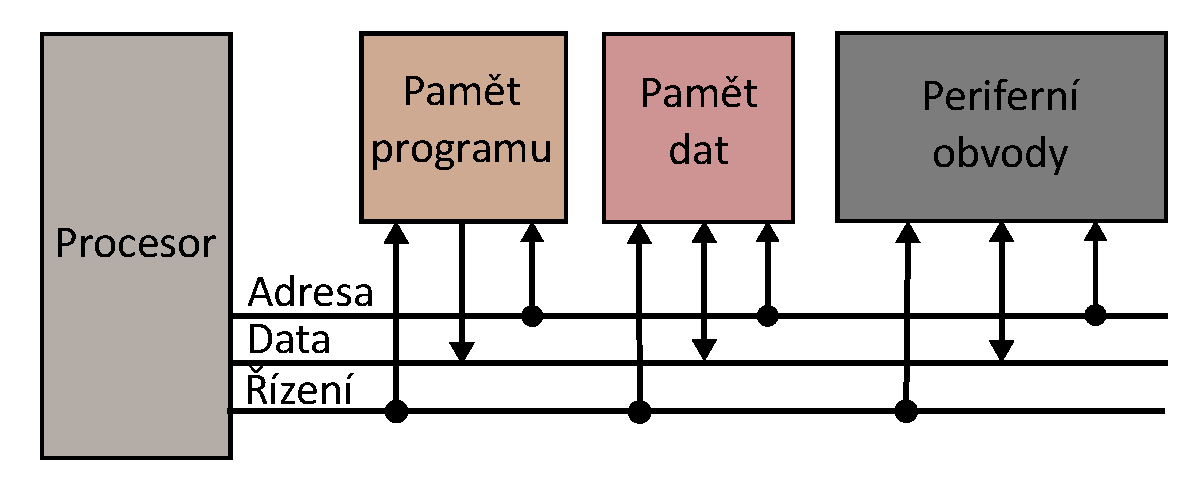
\includegraphics[width=0.9\linewidth]{MCU_arch_basic.pdf}
      \caption{Zjednodušené schéma počítače}
      \label{MIT:fig_pocitac01}
    \end{figure}

    Vzájemné spojení jednotek je v počítači zásadně zprostředkováno soustavou sběrnic (viz obr. 
    \ref{MIT:fig_pocitac01}). \textbf{Sběrnice} umožňují stavebnicovou koncepci, rozšiřování 
    počítače o další jednotky, a to vše beze změn ve vnitřním zapojení jednotek. Negativní stránkou 
    sběrnice je to, že v každém okamžiku na ni může být připojen jen jeden zdroj dat. Nelze tak 
    např. současně předávat data ze dvou zdrojů ke dvěma příjemcům. Činnost sběrnice je v každém 
    okamžiku řízena jen jednou z jednotek - zpravidla je to procesor, ale v některých případech 
    může dočasně přebírat řízení i jiná jednotka. 
    \begin{itemize}\addtolength{\itemsep}{-0.5\baselineskip}
      \item \emph{Datová sběrnice} slouží k předávání dat a její šířka (tj. počet vodičů) je 
            zpravidla celým násobkem osmi (tj. jednoho byte). Jednotka, připojená na sběrnici, může 
            být zdrojem dat (pak se z ní čte), příjemcem dat (pak se do ní zapisuje), nebo střídavě 
            obojím. Jednotka, která je zdrojem dat, se na datovou sběrnici zásadně připojuje 
            prostřednictvím třístavových členů.
      
      \item \emph{Adresová sběrnice} je nutná pro adresování paměti (případně i jiných 
            adresovatelných obvodů) a pro rozlišování mezi jednotkami, připojenými na datovou 
            sběrnici. Šířka adresové sběrnice určuje maximální počet adres. U osmibitových počítačů 
            má adresová sběrnice šířku nejčastěji 16 bitů, u šestnáctibitových počítačů bývá 
            minimálně 20bitová.
      
      \item Čtení, zápis a další aktivity jednotek jsou řízeny signály \emph{řídicí sběrnice}. 
            Většina řídicích signálů je generována procesorem, ale některé mohou být generovány i 
            ostatními jednotkami, které tak mohou částečně ovlivňovat činnost procesoru - takovéto 
            signály jsou pak na řídicí sběrnici připojeny zpravidla přes členy s otevřeným 
            kolektorem. Řídicích signálů bývá obecně větší počet a podoba řídicí sběrnice je silně 
            závislá na celkové architektuře počítače.
    \end{itemize}
    
    Stručně popišme funkci jednotlivých bloků z obr. \ref{MIT:fig_pocitac01}. \textbf{Procesor} 
    řídí činnost celého počítače. Zajišťuje správné provádění \emph{instrukcí} uložených v paměti 
    programu, zpracovává data v paměti, řídí tok dat ze vstupních obvodů do počítače a jejich 
    zpracování, řídí tok dat z počítače ven přes výstupní obvody. Podle počtu bitů zpracovávaných 
    dat se procesor označuje jako osmibitový, šestnáctibitový, dvaatřicetibitový, atd Je třeba 
    poznamenat, že počet bitů procesoru nemusí být shodný se šířkou datové sběrnice. Tak např. 
    některý 16bitový procesor může využívat jen 8bitovou datovou sběrnici. Vnitřní datové slovo (16 
    bitů, tj. 2 byte) pak musí samozřejmě být přenášeno na dvakrát. Takovéto řešení je jednodušší z 
    hlediska obvodů i plošného spoje, činnost počítače však bude pomalejší.
    
    \textbf{Paměť programu} obsahuje instrukce, jejichž postupným prováděním je realizována 
    požadovaná činnost počítače. Dále často obsahuje různé konstanty a neměnné tabulky, používané v 
    programu. Někdy je program pro danou aplikaci neměnný a pak bývá bezpečně uložen v paměti 
    \emph{ROM} (EPROM, EEPROM, FLASH). Jindy se naopak programy potřebují často měnit. To je případ 
    počítače pro vědecko-technické výpočty. Pak musí být programová paměť typu RAM (Random access 
    memory). Je ovšem nezbytné vyřešit otázku, jak spustit program po zapnutí mikropočítače, kdy 
    paměť RAM má zcela náhodný obsah. Proto se počítač i v těchto případech vybavuje malou 
    programovou pamětí ROM. Po náběhu napájení program začíná zde a vyvolá čtení z velkokapacitní 
    diskové paměti. Její obsah (část operačního systému) se přesune do rozsáhlejší programové 
    paměti RAM. Tento program pak přebírá řízení počítače - komunikaci s operátorem, přesunování 
    dalších programů z diskové paměti, jejich spouštění, atd.
    
    \textbf{Paměť dat} zajišťuje dočasné uložení dat, získaných ze vstupních obvodů, uložení 
    mezivýsledků výpočtů apod. Je zásadně typu RAM. Pokud i programová paměť je typu RAM, mohou být 
    případně obě realizovány jedinou společnou paměťovou jednotkou.

    \begin{figure}[ht!] %\ref{MIT:fig_intel4004}
      \centering
      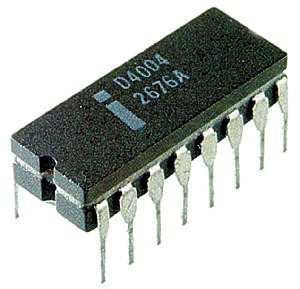
\includegraphics[width=0.5\linewidth]{intel4004.jpg}
      \caption{První komerčně dostupný 4b procesor \texttt{4004} s frekvencí \SI{108}{\kHz} od 
        firmy Intel. Obsahoval 2300 tranzistorů a jeho výkon odpovídal 0.06 MIPS (dále 
        obsahoval 16 4bitových registrů, 45 jedno a dvou bitových instrukcí. čtyř úrovňový 
        adresový zásobník a 12bitový programový čítač. Procesor musel být doplněn čtyřmi 
        dalšími podpůrnými obvody 4001 až 4004.}
      \label{MIT:fig_intel4004}
    \end{figure}
    \textbf{Vstupní a výstupní obvody (l/O - Input/Output)} umožňují počítači komunikovat s vnějším 
    prostředím. Zpravidla obsahují větší počet bran (angl. port), tj. připojovacích míst, 
    rozlišených adresově. Brány mohou být paralelní nebo sériové. Při paralelním přenosu se čte 
    nebo zapisuje najednou celá skupina signálů jako vícebitové slovo (např. 8bitové). Při sériovém 
    přenosu se data přenášejí postupně bit po bitu. Sériový přenos je mnohem pomalejší než 
    paralelní, ale je úspornější co se týče počtu signálových vodičů.

    Výše popsaná struktura platí obecně pro všechny počítače. Pokroky v technologii integrovaných 
    obvodů umožnily zmenšení rozměrů a koncentraci mnoha funkcí do jednoho integrovaného obvodu 
    VLSI. Vznikl tak pojem \textbf{mikropočítače} a \textbf{mikroprocesoru}. Je nutné zdůraznit, že 
    předpona „mikro" se vztahuje k fyzický rozměrům obvodů a neznamená omezení funkce. Právě 
    naopak, vysoká integrace umožnila vývoj velmi složitých architektur s vysokým výpočetním 
    výkonem a velkou variabilitou funkcí. Soustředění obvodů na jednom čipu dovoluje zkrátit spoje 
    a tím i zpoždění signálu.   
       
    Vůbec první procesor s názvem \wikiIntelfirst v podobě jak ho známe dnes představila firma 
    \wikiIntelCompany roku 1971. Tento procesor ovšem ke své funkci potřeboval další podpůrné 
    obvody (Intel 4001 až 4004). S postupující integrací bylo možné sdružit všechny obvody 
    mikropočítače do jediného integrovaného obvodu. Vznikla tak řada \textbf{jednočipových 
    mikropočítačů}. Zvláště v této skupině počítačů probíhá nejintenzivnější vývoj. Zvětšuje se 
    kapacita paměti programu i paměti dat, rozšiřuje se sestava periferních obvodů. Jednočipový 
    mikropočítač, vhodný pro využití v řízení, je v anglické literatuře označován jako 
    „\textbf{mi\-cro\-con\-tro\-ller}", česky \emph{mikrokontrolér}.
    
    Počítače pronikly do všech oblastí života a jsou součástí měřicích přístrojů, vozidel, 
    audiovizuálních přístrojů, mobilních telefonů, atd. Počítače v těchto aplikacích jsou v 
    anglické literatuře označovány jako „\textbf{embedded computers}", v českém překladu 
    \emph{zabudované} nebo \emph{vložené počítače}.
    
    Vývoj nových typů mikrokontrolérů využívá technologii \textbf{ASIC}, založenou na sdružování a 
    sestavování masek\footnote{slouží v procesu fotolitografie} pro výrobu integrovaných obvodů. 
    Dílčí masky odpovídají osvědčeným, ověřeným jednotkám počítače. Podle potřeby se pak sestaví 
    jádro počítače (procesor a k němu přilehlé obvody), paměti a několik variant sestavy 
    periferních obvodů - vše integrováno na jednom čipu. Vznikají tak \textbf{rodiny 
    mikropočítačů}, které mají společné jádro.
    
    Na rozdíl od rychlého vývoje sestav periferních obvodů a zvyšování kapacity vnitřní paměti je 
    vývoj nových procesorů podstatně konzervativnější. Souvisí to s nutností kompatibility (tj. 
    slučitelnosti) programů po dlouhou dobu. Finanční prostředky, investované do vývoje programů, 
    jsou obrovské a žádný výrobce integrovaných obvodů tuto skutečnost nemůže ignorovat. 
    Modernizace procesoru se děje nejčastěji přidáváním několika málo instrukcí, zvýšením 
    rychlosti, doplněním o specializované obvody. Kompatibilita programů je tak zaručena směrem 
    nahoru (programy pro starší verzi jsou plně použitelné i pro verzi 
    novou), ale ne nutně směrem dolů.
    
    \subsection{Sběrnicové cykly}
      Jak bylo výše řečeno, přenosy dat v počítači probíhají po sběrnicích. Obecný pohled na 
      jednotku, připojenou na sběrnice, dává obr. \ref{MIT:fig_bus_cycle}.
      
      \begin{figure}[ht!] %\ref{MIT:fig_bus_cycle}
        \centering
        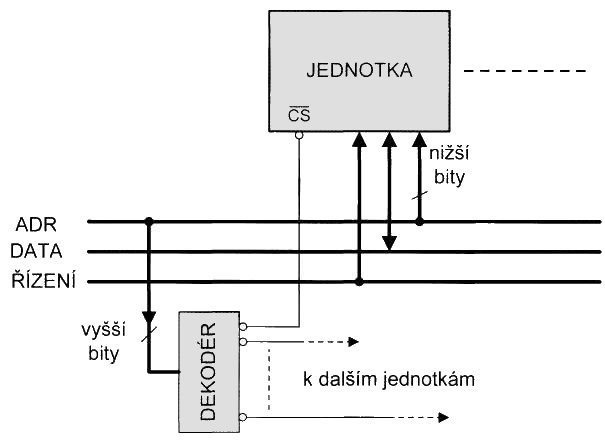
\includegraphics[width=0.95\linewidth]{bus_cycle.jpg}
        \caption{ Připojení jednotky na sběrnice}
        \label{MIT:fig_bus_cycle}
      \end{figure}
      Nejvyšší bity adresy jsou vedeny do \emph{adresového dekodéru}, jehož výstupy (v kódu 1 z N) 
      vybírají jednu z jednotek a povolují její činnost. Pokud je jednotkou samotný integrovaný 
      obvod, bude se zřejmě jednat o jeho vstup \texttt{CS}. Pro jednoduchost budou výběrové 
      signály na výstupech dekodéru takto nazvány i v obecném případě. V jednotce jsou využity 
      zbylé (nižší) bity adresy pro adresování uvnitř obvodů v rámci této jednotky (např. paměti).
      
      Datová sběrnice je obecně dvousměrná a jednotka, připojená na sběrnici, může být jen zdrojem 
      dat (pak se z ní jen čte, např. paměť ROM), příjemcem dat (pak se do ní jen zapisuje, např. 
      výstupní obvody), nebo střídavě obojím (např. paměť RAM). Směr čtení/zápis se rozlišuje vždy 
      z pohledu od procesoru. Čtení i zápis jsou řízeny a přesně časovány prostřednictvím signálů 
      řídicí sběrnice. Zatím je označíme jako  a \textoverline{\texttt{WR}}. Aktivním stavem je 
      zpravidla „L" (low, nízká úroveň) proto jsou v negaci. Řídicích signálů však může být větší 
      počet - např. vstupní a výstupní obvody mohou mít své řídicí signály jiné než paměť.
      
      Posloupnost činností, během kterých dojde právě jednou ke čtení nebo zápisu prostřednictvím 
      sběrnic, se nazývá \emph{\textbf{sběrnicový cyklus} (angl. bus cycle)}. Základními 
      sběrnicovými cykly jsou cyklus čtení z paměti a cyklus zápisu do paměti. Vedle toho mohou 
      existovat i další sběrnicové cykly, jako např. čtení ze vstupních obvodů, zápis do výstupních 
      obvodů, aj. Časování signálů může být v těchto cyklech odlišné.
      
      Pokud má být rychlost procesoru i dalších obvodů počítače využita na maximum, musí být 
      časování velmi přesné. To je zajištěno synchronizací procesoru generátorem hodinových 
      impulzů, řízeným krystalem.

    \subsection{Periferní obvody}
      Periferní obvody tvoří velmi rozmanitou skupinu obvodů, zvlá\-ště u počítačů využitých pro 
      řízení. I přes jejich rozmanitost však lze nalézt obecně platné vlastnosti. Velmi často je 
      několik periferních obvodů sdruženo (integrováno) dojedná periferní jednotky např. několik 
      paralelních bran, několik sériových bran, několik čítačů a časovačů, vícekanálový převodník 
      A/Č, apod. Zjednodušené schéma periferní jednotky ukazuje obr. \ref{MIT:fig_periferie}.
      \begin{figure}[ht!] %\ref{MIT:fig_periferie}
        \centering
        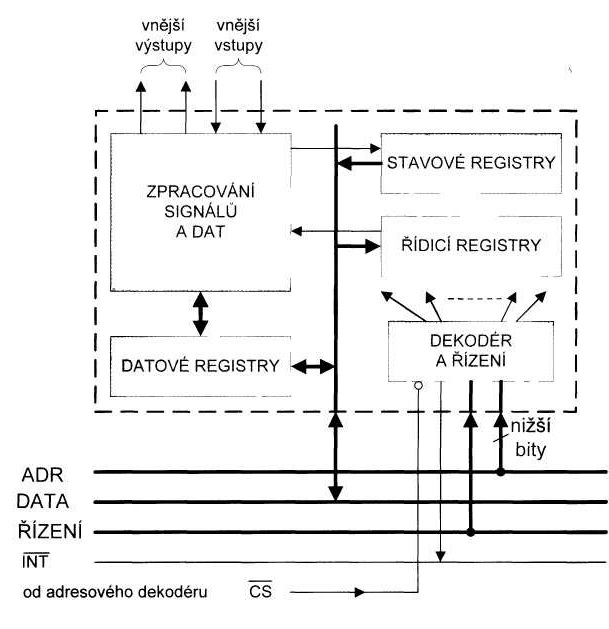
\includegraphics[width=0.95\linewidth]{periferie.jpg}
        \caption{Zjednodušené schéma periferní jednotky}
        \label{MIT:fig_periferie}
      \end{figure}
      
      Jádrem periferní jednotky jsou obvody pro zpracování signálů. To jsou např. čítače, 
      převodníky, nebo třeba jen jednoduché výkonové oddělovací členy. Ze strany datové sběrnice s 
      nimi komunikuje procesor, z druhé strany pak okolí počítače. Jelikož v jednotce bývá sdruženo 
      několik periferních obvodů, jsou data ukládána do několika datových registrů.
      
      Velmi často je nutné činnost těchto obvodů nějak řídit - nastavit cesty signálů, dělicí 
      poměry čítačů, různé vnitřní vazby, apod. K tomu slouží skupina \emph{řídicích registrů}. 
      Dále je třeba zjišťovat stav těchto obvodů - např. přetečení čítače, skončení A/Č převodu, 
      přijetí znaku v sériovém přenosu, apod. K tomu slouží skupina \emph{stavových registrů}. 
      Procesor může prostřednictvím datové sběrnice zapisovat do řídicích registrů a číst stavové 
      registry. \emph{U jednočipových mikropočítačů jsou řídicí a stavové registry seskupeny v 
      jedné oblasti vnitřní paměti}.
      
      Jednotka může vyžadovat obsluhu též prostřednictvím přerušení programu. K tomu slouží jeden 
      nebo více signálů \texttt{INT}. Podnětem k vyvolání přerušení je dokončení požadované operace 
      (dokončení A/Č převodu, přijetí znaku v sériovém přenosu, atd.) nebo případné hlášení chyby 
      (zvláště v komunikačních obvodech). Do jednotky je vedeno několik (nejnižších) adresových 
      bitů pro rozlišení mezi různými datovými, řídicími a stavovými registry. Uvnitř jednotky 
      zřejmě musí existovat ještě lokální adresový dekodér. Signál \textoverline{\texttt{CS}} 
      (pokud vůbec existuje) blokuje vždy jen komunikaci s jednotkou ze strany sběrnic, nikdy 
      neblokuje činnost vnitřního jádra, ani vnějších vstupních a výstupních signálů, ani vyvolání 
      přerušení.
      
    \subsection{Adresový prostor}\label{MIT:chap_adr_prostor}
      Adresový prostor je \emph{množina adres}, na které lze dosáhnout jedním typem sběrnicového 
      cyklu. Tak může existovat \emph{programový prostor, datový prostor, vstupní/ výstupní 
      prostor}, atd. Existuje několik uspořádání adresových prostorů, která úzce souvisejí s 
      architekturou počítače, se složením řídicí sběrnice, a též s instrukčním souborem procesoru.
      
      Adresové prostory lze velmi snadno znázornit, jak ukazuje obr. \ref{MIT:fig_adrspace1}. Jedná 
      se v tomto případě o \textbf{počítač s jediným adresovým prostorem}, do kterého jsou vloženy 
      dílčí prostory  - programový, datový a periferní. Adresy rostou směrem zdola nahoru (v 
      některých publikacích je zvolen opačný směr). Co se týče obvodového řešení, je zahrnutí všech 
      obvodů do jednoho prostoru docíleno jedním adresovým dekodérem, který aktivuje vždy jednu 
      skupinu obvodů (např. paměť \texttt{ROM}, paměť \texttt{RAM}, periferní obvody) a společným 
      rozvodem řídicích signálů  a  \textoverline{\texttt{WR}} do všech obvodů (s výjimkou do ROM, 
      kde zřejmě signál \textoverline{\texttt{WR}} pro řízení zápisu nemá smysl). Existují tedy 
      zásadně jen dva sběrnicové cykly - čtení a zápis. Obvodové uspořádání ukazuje obr. 
      \ref{MIT:fig_adrspace1}. K výběru obvodů jsou využity nejvyšší bity adresy. Tato architektura 
      se nazývá \textbf{von Neumannova}. Výhodou je jednoduché řízení obvodů počítače.
      
      \begin{figure}[ht!]
        \centering  
        \begin{tabular}{cc}
          \subfloat[obsazení adr. prostoru]{\label{MIT:fig_adrspace1}
            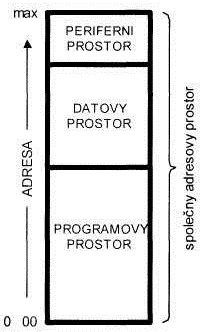
\includegraphics[width=0.3\linewidth]{adresovy_prostor1.jpg}}              &
          \subfloat[obvodové uspořádání]{\label{MIT:fig_adrspace2}
            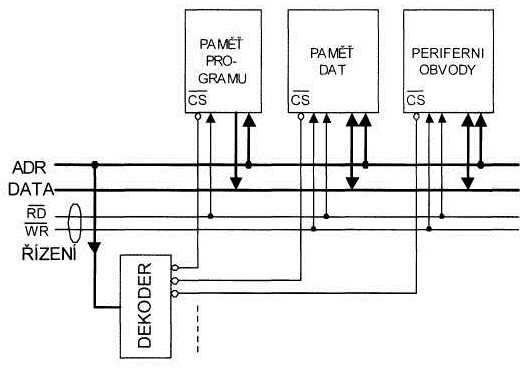
\includegraphics[width=0.6\linewidth]{adresovy_prostor2.jpg}}              \\
        \end{tabular}
        \caption{Počítač s jedním adresovým prostorem}
      \end{figure}

      Jinou možnost ukazuje obr. \ref{MIT:fig_adrspace3}. V počítači existuje \textbf{několik 
      adresových prostorů} (např. programový, datový, periferní), ne nutně stejně rozsáhlých. V 
      několika různých adresových prostorech mohou existovat stejné adresy. K rozlišení prostorů 
      tedy nemůže sloužit adresa, ale \textbf{typ sběrnicových cyklů}. Jsou to zásadně tyto: 
      \emph{čtení instrukce, čtení dat, zápis dat, čtení z periferních obvodů, zápis do periferních 
      obvodů}, případně některé další. Větší počet sběrnicových cyklů vyžaduje také větší počet 
      řídicích signálů - např. tak, jak je naznačeno v obr. \ref{MIT:fig_adrspace4}. Uvedená 
      soustava řídicích signálů není jedinou, existují i jiné - detaily jsou v dalších kapitolách. 
      Rozlišení cyklu čtení instrukce a čtení dat nečiní potíže, neboť se zřejmě jedná o úplně jiné 
      operace procesoru. Jinak je tomu s rozlišením cyklu čtení dat a čtení z periferních    
      obvodů, či rozlišením zápisu dat a zápisu do periferních obvodů. Toto rozlišení je možné jen 
      tak, že bude existovat jiný soubor instrukcí pro práci s datovou pamětí a jiný pro práci s 
      periferními obvody. V závislosti na typu instrukce pak procesor zvolí patřičný typ 
      sběrnicového cyklu. Výhodou je větší celkový počet adres.
      
      \begin{figure}[ht!]
        \centering  
        \begin{tabular}{cc}
          \subfloat[obsazení adr. prostoru]{\label{MIT:fig_adrspace3}
            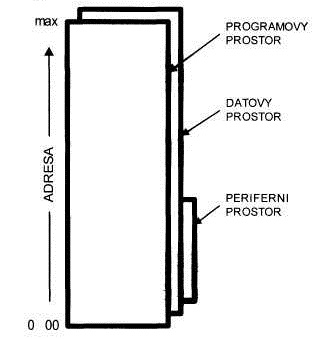
\includegraphics[width=0.3\linewidth]{adresovy_prostor3.jpg}}              &
          \subfloat[obvodové uspořádání]{\label{MIT:fig_adrspace4}
            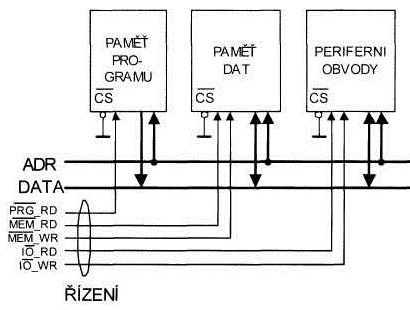
\includegraphics[width=0.6\linewidth]{adresovy_prostor4.jpg}}              \\
        \end{tabular}
        \caption{Počítač s několika adresovými prostory}
      \end{figure}
      
      Tato architektura může být dále rozvíjena pro realizaci velmi rychlých počítačů. Sběrnice je 
      vždy omezujícím prvkem co do rychlosti, neboť nedovoluje současné přenosy ze dvou nebo více 
      zdrojů dat (zkraty na výstupech třístavových budičů sběrnice). Procesor by sice mohl současně 
      zapisovat data (jako výsledek právě ukončené instrukce) a současně s tím číst novou 
      instrukci, architektura s jedinou soustavou sběrnic to však nedovoluje. Proto byla zavedena 
      architektura se dvěma soustavami sběrnic. Na jednu je připojena paměť programu, na druhou 
      paměť dat (případně další obvody) - viz obr.\ref{MIT:fig_adrspace5}.

      \begin{figure}[ht!] %\ref{MIT:fig_adrspace5}
        \centering
        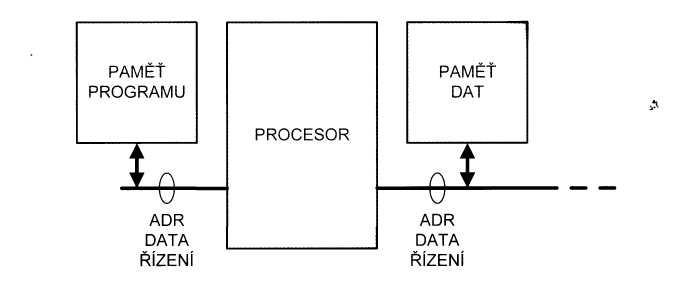
\includegraphics[width=0.7\linewidth]{adresovy_prostor5.jpg}
        \caption{Počítač s dvěma soustavami sběrnic}
        \label{MIT:fig_adrspace5}
      \end{figure}
      
      Popsaná architektura je známá pod názvem \textbf{harvardská} a je důsledně aplikována zvláště 
      u \emph{signálových procesorů}.
      
      Název pochází z počítače \texttt{Harvard Mark I}, který byl postaven na této architektuře. 
      Tento počítač měl strojové instrukce uloženy na děrované pásce (šířka 24 bit) a data na 
      elektro-mechanických deskách (23 číslic široké).      
      
  \section{Procesor}
    Úkolem \emph{procesoru} je provádění \textbf{instrukcí}. Instrukce jsou nej\-men\-ší jednotky, 
    ze 
    kterých je složen program. Základní části instrukce jsou znázorněny na obr. 
    \ref{MIT:fig_instrukceOP}. Ve všech případech je první částí \textbf{operační kód} \emph{(angl. 
    op-code, též operační znak, instrukční kód)}. Ten přesně definuje další činnost při provádění 
    instrukce.
    \begin{figure}[ht!]
      \centering  
      \begin{tabular}{ccc}
        \subfloat[ ]{\label{MIT:fig_instrukce1a}
          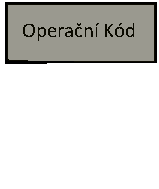
\includegraphics[width=0.2\linewidth]{instrukce1a.pdf}}                    &
        \subfloat[ ]{\label{MIT:fig_instrukce1b}
          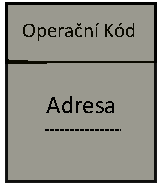
\includegraphics[width=0.2\linewidth]{instrukce1b.pdf}}                    &
        \subfloat[ ]{\label{MIT:fig_instrukce1c}
          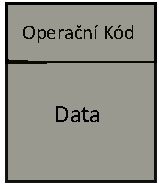
\includegraphics[width=0.2\linewidth]{instrukce1c.pdf}}                   \\
      \end{tabular}
      \caption{Počítač s několika adresovými prostory}
      \label{MIT:fig_instrukceOP}
    \end{figure}

    Některé instrukce (viz případ na obr. \ref{MIT:fig_instrukce1a} obsahují jen \emph{operační 
    kód}. V těchto případech jsou prováděny jen vnitřní operace v procesoru - např. „inkrementuj 
    obsah vnitřního datového registru apod. V druhém případě (obr. \ref{MIT:fig_instrukce1b}) 
    obsahuje instrukce ještě \emph{adresu operandu}. Operandy jsou uloženy v datové paměti. 
    Příkladem mohou být instrukce typu „přesuň obsah vnitřního datového registru do datové paměti 
    na adresu..." apod. Ve třetím případě (obr. \ref{MIT:fig_instrukce1c}) obsahuje instrukce ještě 
    \emph{přímá data}. Jedná se vždy o konstanty, které jsou součástí programu. Příkladem může být 
    instrukce „naplň vnitřní datový registr číslem ...".
    
    Existují i složitější instrukce obsahující dvě nebo tři adresy, adresu i data apod. - záleží 
    vždy na instrukčním souboru procesoru. \emph{Instrukce mají tedy obecně různou délku}. Celý 
    průběh instrukce se skládá ze dvou fází - přečtení instrukce a provedení instrukce. 
    \textbf{Přečtení instrukce} znamená vyvolání čtecích cyklů z paměti programu při postupně 
    rostoucích adresách tak, aby se postupně přečetly všechny části instrukce Počet čtecích cyklů 
    odpovídá délce instrukce. \textbf{Adresa instrukce} odpovídá adrese, na které je uložen 
    operační kód. Provedení instrukce znamená vykonání vnitřních operací v procesoru včetně získání 
    potřebných operandů z datové paměti (jsou-li operandy v instrukci definovány) a následné 
    uložení výsledků do datové paměti (je-li to v instrukci vyžadováno). Jako příklad může sloužit 
    instrukce „inkrementuj obsah paměti na adrese...", jejíž provádění je následující - viz obr. 
    \ref{MIT:fig_intrukce}.

    \begin{figure}[ht!] %\ref{MIT:fig_intrukce}
      \centering
      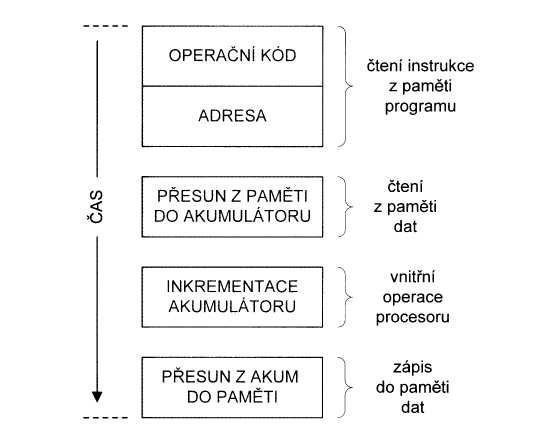
\includegraphics[width=0.7\linewidth]{instrukce2.jpg}
      \caption{Příklad činnosti při provádění instrukce}
      \label{MIT:fig_intrukce}
    \end{figure}
    
    Z výše uvedeného již vyplývají některé potřebné obvody v procesoru. Předně je to \textbf{čítač 
    instrukcí PC} (angl. \emph{Program Counter}), který slouží k adresování paměti programu. Čítač 
    je postupně inkrementován a program je tak postupně čten. Dále je to \textbf{instrukční registr 
    IR}, do kterého je uložen operační kód. Na základě obsahu IR je dále řízen průběh provádění 
    instrukce. Má-li instrukce adresovou část, je tato uložena do \textbf{pomocného adresového 
    registru TAR} (angl. \emph{Temporary Address Register}), který bude během následujícího 
    provádění instrukce dodávat adresu pro paměť dat. Pokud instrukce obsahuje datovou část, je 
    tato uložena do \textbf{pomocného datového registru TDR}, kde bude k dispozici během provádění 
    instrukce. Tyto (a mnohé další) pomocné registry jsou uživateli zpravidla nedostupné a 
    neviditelné. Vnitřní obvody si předávají data po vnitřní datové sběrnici.
    
    Další registry, využívané pro tvorbu adresy, jsou \textbf{indexregistry} Některé jednoduché 
    procesory je nemají, ale většinou jsou alespoň dva. Obsah indexregistru může být v některých 
    instrukcích přičten k obsahu adresové části instrukce a tento součet je teprve použit jako 
    adresa pro paměť. \emph{Indexová adresace} je výhodná pro práci s tabulkami, řetězci a poli.
    
    Operace s daty (aritmetické a logické operace) jsou prováděny v \textbf{aritmeticko-logické 
    jednotce ALU} (angl. \emph{Arithmetic-Logic Unit}). Výsledek ve tvaru binárního čísla je uložen 
    do \textbf{střadače} (též \emph{akumulátoru}) \textbf{A} (angl. \emph{Accumulator}). To však 
    není jediný výsledek - cenná může být i informace o nulovosti přenosu z nejvyššího bitu, 
    přetečení rozsahu čísla atd. Všechny tyto informace jsou ve své podstatě jednobitové. Tyto 
    \textbf{příznakové bity} (angl. Flags) jsou uloženy do \textbf{registru příznaků F} (též 
    \textbf{CCR} - z angl. \emph{Condition Code Register}). Jednotlivé bity mohou sloužit např. 
    jako \emph{podmínky pro větvení programu}.
    
    Pro krátkodobé uložení dat slouží několik \textbf{datových registrů} (\textbf{GPR} - angl. 
    \emph{General Purpose Register}), neboli registrů \textbf{zápisníkové paměti}. Jelikož jsou 
    uvnitř procesoru, je přístup k nim rychlejší než k vnější datové paměti. Tyto registry 
    zpravidla plní i jiné úkoly - např. některé mohou sloužit k adresaci datové paměti, k 
    odpočítávání počtu opakování programových smyček atd.
    
    Řízení vnitřních obvodů - nastavení cest dat, zápisy do registrů, řízení operací ALU atd. - 
    provádí \textbf{řadič}\footnote{každý řadič je totiž ve skutečnosti konečným automatem, který 
    se může nacházet vždy v jednom z konečného počtu stavů} (angl. \emph{Controller}). Jedná se 
    vždy o velmi složitý \emph{sekvenční 
    obvod}, řešený buď jako:
    \begin{itemize}\addtolength{\itemsep}{-0.5\baselineskip}
      \item \emph{obvodový řadič} - pevně zapojená logika - obsahuje buď čítač nebo posuvný 
           registr. Ovšem použití obvodového řadiče začíná být ekonomicky i z časového hlediska 
           (doba vývoje nového mikroprocesoru) nevýhodné v případě, že má mikroprocesor složitější 
           architekturu  (větší množství interních sběrnic, více ALU, pipelining, atd.)
      \item \hyperlink{MIT:sec_001}{mikroprogramo­vaného řadiče} - jehož nedílnou součástí je 
             řídicí paměť obsahující 
             mikroinstrukce, přičemž každá ze strojových instrukcí je provedena pomocí několika 
            jednodušších mikroinstrukcí.
    \end{itemize} 
   
    Jednotlivé posloupnosti řídicích signálů, generované řadičem, jsou vyvolávány 
    \textbf{instrukčním dekodérem ID}, který na základě obsahu IR rozliší typ instrukce a tomu 
    přiřadí patřičný počáteční stav sekvenčního obvodu řadiče (či nastaví počáteční adresu 
    mikroprogramu v paměti mikroprogramů).    
    
    \begin{figure}[ht!] %\ref{MIT:fig_procesor}
      \centering
      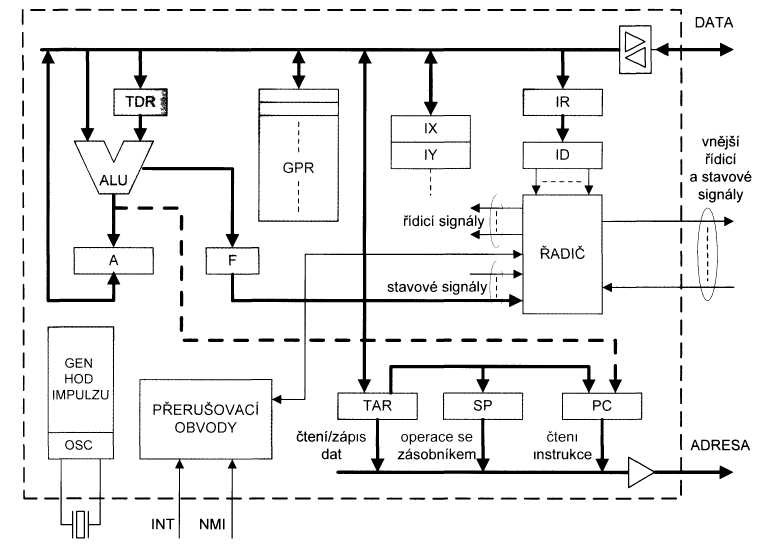
\includegraphics[width=1\linewidth]{procesor.jpg}
      \caption{Základní obvody procesoru}
      \label{MIT:fig_procesor}
    \end{figure}
    
    \begin{note}      
      Koncepce řadiče na základě mikroprogramového automatu umožňuje konstruktérovi procesoru 
      snadnou modifikaci instrukčního souboru pouhou změnou obsahu paměti mikroprogramů bez dalších 
      zásahů do architektury procesoru. Naopak řadič, navržený jako pevně zapojená sekvenční 
      logika, umožňuje rychlejší činnost.
    \end{note}
    
    Řadič inkrementuje obsah \texttt{PC} tak, aby byly postupně čteny všechny části instrukce a aby 
    byla na konci čtení instrukce k dispozici již adresa následující instrukce. Tak jsou čteny a 
    zpracovávány instrukce s postupně rostoucí adresou v paměti programu. Výjimku tvoří instrukce 
    skoku a volání podprogramů. Ty mají svoji adresovou část, která se přečte a dočasně uloží do 
    TAR. Obsah TAR se pak přesune do \texttt{PC}.
    
    Některé instrukce jsou \textbf{podmíněné} (např. \emph{podmíněné skoky}) v tom smyslu, že jsou 
    provedeny jen při splnění jisté podmínky. Jako podmínky slouží stavy jednotlivých bitů registru 
    \texttt{F}. Příznakové bity jsou zavedeny do řadiče, kde modifikují průběh mikroprogramu. Výběr 
    podmínky je dán tvarem operačního kódu. Tak např. existuje podmíněný skok při splnění 
    podmínky nulovosti výsledku předcházející operace \texttt{ALU}, atd. Při nesplnění podmínky se 
    čte instrukce z následující adresy v programové paměti.
     
    \textbf{Ukazatel zásobníkové paměti SP} (angl. \emph{Stack Pointer}) slouží pro adresování 
    zásobníku (Stack). Zásobník zaujímá část datové paměti. Při operacích se zásobníkem se v 
    programu neudává adresa. Jedná se o paměť typu \emph{LIFO} (z angl. \emph{Last In - First 
    Out}). Adresa je uložena v \texttt{SP}, který je řadičem inkrementován nebo dekrementován, 
    takže zásobník při vkládání dat postupuje na jednu stranu a při vybírání dat na druhou stranu - 
    rozhodující pro růst zásobníku je postup při zápisu. Obr. \ref{MIT:fig_ukazatel} ukazuje 
    architekturu procesoru, při které zásobník \emph{postupuje dolů}, směrem k nižším adresám. Je 
    třeba upozornit, že u některých procesorů zásobník naopak \emph{postupuje nahoru}. Bez 
    ohledu na směr postupu zásobníku je jeho vrcholem (angl. \emph{top}) nazývána adresa, na kterou 
    ukazuje \texttt{SP} a dnem (angl. \emph{bottom}) adresa, na kterou byla uložena první data.
    
    
    \begin{figure}[ht!] %\ref{MIT:fig_ukazatel}
      \centering
      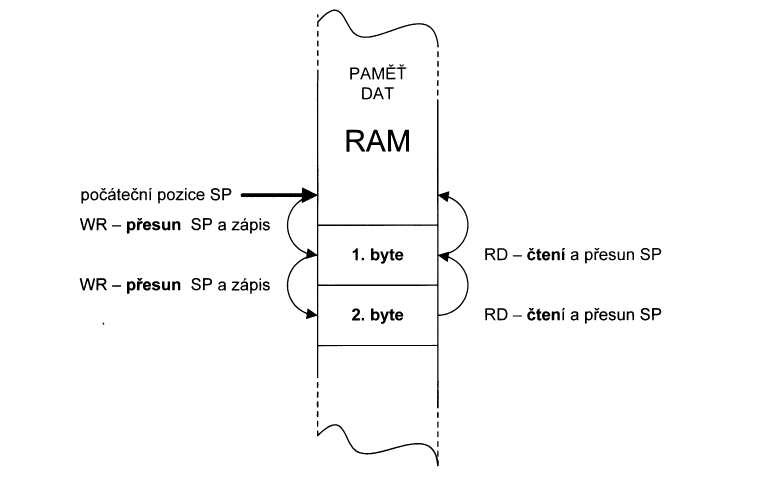
\includegraphics[width=0.8\linewidth]{ukazatel.jpg}
      \caption{Adresace při postupném zápisu a čtení dvou slabik}
      \label{MIT:fig_ukazatel}
    \end{figure}
    
    U moderních procesorů se při zápisu do zásobníku SP nejprve posune a teprve pak je jeho obsah 
    použit jako adresa pro zápis do \texttt{RAM}. Při čtení ze zásobníku je adresa dána obsahem SP, 
    který se teprve po čtení posune. \texttt{SP} tak ukazuje na poslední data uložená do zásobníku. 
    Ukazatel zásobníku lze přednastavit instrukcí \emph{„naplň SP číslem ..."} a tím lze založit 
    zásobník v požadované oblasti datové paměti.
    
    Výše uvedená činnost zásobníku je typická pro instrukce \emph{„ulož data do zásobníku"} a 
    \emph{„vyber data ze zásobníku"}. Zásobník má však ještě druhou důležitou funkci a to 
    \textbf{zapamatování adres návratu}. K tomu dochází automaticky při volání podprogramů 
    instrukcí \emph{„volej podprogram na adrese ..."}. Po přečtení instrukce je její adresová část 
    dočasně uložena v TAR a PC je inkrementován, takže ukazuje na následující instrukci. Obsah PC 
    je vložen do zásobníku a pak je do PC přesunut obsah \texttt{TAR}. Program tím pokračuje na 
    nové adrese (mimo původní pořadí). Podprogram je zakončen instrukcí \emph{„návrat z 
    podprogramu"}. Tato instrukce způsobí automatické vybrání obsahu zásobníku a jeho přesun 
    do PC. Program proto dále pokračuje tam, odkud byl vytržen instrukcí volání podprogramu. Tento 
    mechanizmus zaručuje, že podprogram lze volat z libovolných míst programu a vždy je zaručen 
    správný návrat. Adresa zapsaná do zásobníku se běžně nazývá \emph{„návratová adresa"}. Přesně 
    vzato je to ale adresa pokračování v původním programu. Uchování návratové adresy a její opětné 
    zavedení je u všech procesorů zcela automatické a pro programátora neviditelné.
    
    Je samozřejmé, že před prvním odskokem na podprogram instrukcí \emph{„volej podprogram na 
    adrese ...."} musí být definován začátek zásobníku, tj. musí být naplněn ukazatel SP vhodným 
    číslem.
    
    Funkce zásobníku umožňuje vložení podprogramů do podprogramů v prakticky libovolném počtu 
    úrovní. Přitom jsou do zásobníku postupně ukládány návratové adresy a při návratech z 
    podprogramů jsou postupně ze zásobníku vybírány. To přesně odpovídá činnosti paměti 
    \texttt{LIFO} - viz obr. \ref{MIT:fig_podprogram}.
    
    Používání zásobníku není bez jistého rizika. Jelikož zásobník je vytvořen v datové paměti, může 
    dojít k jeho kolizi s datovou oblastí. Hloubka zásobníku (tj. počet vložených údajů) nemusí být 
    předem přesně známa, jak je tomu např. při využívání převzatých knihoven podprogramů bez 
    dostatečné dokumentace, při rekurentních programech, při podmínečných voláních podprogramů. 
    Příliš \emph{„narostlý"} zásobník může přepsat data, ale horší případ nastane, když naopak data 
    přepíší obsah zásobníku. Tím jsou ztraceny návratové adresy a zhroucení celého programu je 
    nevyhnutelným důsledkem.    
    
    \begin{figure}[ht!] %\ref{MIT:fig_podprogram}
      \centering
      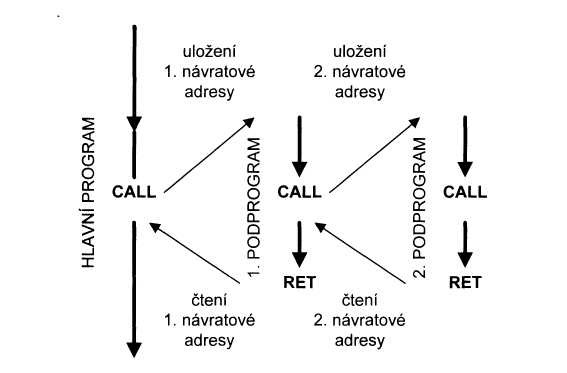
\includegraphics[width=0.7\linewidth]{podprogram.jpg}
      \caption{Ukládání adres při vložených podprogramech}
      \label{MIT:fig_podprogram}
    \end{figure}
    
    Velmi důležitou součástí procesoru jsou obvody pro zpracování \textbf{přerušení} programu 
    (angl. \emph{Interrupt}). Přerušení je vyvoláno vnitřními obvody procesoru při výjimečných 
    stavech (např. dělení nulou, chyba při čtení instrukce, apod.) nebo též vnějšími signály a 
    vyvolá odskok na podprogram. Rozdíl mezi vyvoláním podprogramu instrukcí \emph{„volání 
    podprogramu"} a vyvoláním podprogramu přerušením spočívá v tom, že k přerušení může dojít 
    \emph{kdykoli}. Jedná se tedy o okamžitou změnu činnosti počítače jako reakci na neočekávaný 
    vnější podnět. Adresa návratu z podprogramu je v obou případech uchována v zásobníku. Přerušení 
    může být \textbf{maskovatelné} nebo \textbf{nemaskovatelné}. Procesor je pak vybaven zvláštními 
    vstupy pro maskovatelné přerušení (\textbf{INT}) a pro nemaskovatelné přerušení   
    (\textbf{NMI}, angl. \emph{Non-Maskable Interrupt}). U maskovatelných přerušení může být podnět 
    blokován v závislosti na stavu vnitřního maskovacího (blokovacího) klopného obvodu. Blokování 
    lze programově nastavovat či nulovat, kromě toho se v některých stavech procesoru přerušení 
    blokuje automaticky. \emph{Nemaskovatelné přerušení nelze blokovat a má přednost před 
    přerušením maskovatelným}.
    
    K počítači je zpravidla připojen větší počet zařízení, která čas od času vyžadují obsluhu 
    prostřednictvím přerušení. Každému z nich přísluší patřičný obslužný podprogram. Počítač musí 
    identifikovat zdroj požadavku na přerušení, rozhodnout o prioritě při případném konfliktu (tj. 
    při současném výskytu více požadavků), určit adresu obslužného podprogramu a provést odskok. 
    Celou tuto činnost nevykonává procesor samostatně, nýbrž zpravidla využívá vnější obvody pro 
    zpracování přerušení (\textbf{řadič přerušení}). Nemaskovatelné přerušení vyvolává odskok na 
    \emph{jedinou} pevně stanovenou adresu bez spoluúčasti dalších obvodů, reakce je tak rychlejší. 
    Návrat z podprogramu je záležitostí programátora, který zakončí obslužný podprogram instrukcí 
    \emph{„návrat z interruptového podprogramu"}.
    
    Obdobně jako v případě volání podprogramu, i při přerušení musí již být předem správně nastaven 
    začátek zásobníku, tj. naplněn ukazatel SP - do té doby musí být přerušení zakázána (blokována).
    
    V podprogramu se většinou pracuje s registry zápisníkové paměti, ve kterých se tím přepíší 
    data, uložená do nich v programu, ze kterého se odskočilo do podprogramu. Po návratu tak může 
    dojít k chybě. To platí zvláště v případě přerušení, které obecně může nastat kdykoliv, bez 
    zásahu a bez vědomí programátora. Na začátku podprogramu je proto nutné obsah pracovních 
    registrů \emph{„uklidit"} instrukcemi \emph{„ulož data do zásobníku"} a na konci podprogramu 
    pak zpětně obnovit instrukcemi \emph{„vyber data ze zásobníku"}. Tento \textbf{úklid} a 
    \textbf{návrat} představuje \emph{časové ztráty}, ale bez změny architektury procesoru je 
    nevyhnutelný.
    
    Pro omezení časových ztrát byla proto vyvinuta architektura se zdvojenou nebo i vícenásobnou 
    zápisníkovou pamětí-tzv. \textbf{registrové banky}. V každém okamžiku je využívána jen jedna 
    banka. Mohou však být přepínány prostřednictvím jednoho nebo více bitů registru, nazvaného 
    \textbf{přepínač bank} (angl. \emph{bank switch}). Zásahem do tohoto registru lze přepnout 
    registrovou banku a pracovat s další skupinou registrů, aniž by obsah předchozí skupiny mohl 
    být porušen. Ve vhodném okamžiku lze přepnout zpět. To se využívá např. v podprogramech 
    (zvláště interruptových), kdy v podprogramu se využívá jiná banka, než ve volajícím programu. 
    Obsah registrů, využívaných ve volajícím programu, tak je po návratu dále k dispozici. Celé 
    přepnutí je záležitostí jen jedné krátké instrukce.
    
    Registr příznaků CCR a další bity, důležité pro řízení činnosti procesoru, jako je např. bit 
    pro blokování přerušení, přepínač bank registrů apod., jsou seskupeny do \textbf{stavového 
    slova programu \texttt{PSW}} (angl. \emph{Program Status Word}). \texttt{PSW} lze jako jeden 
    celek ukládat do zásobníku na začátku podprogramu (zvláště interruptového) a na konci 
    podprogramu je lze opět ze zásobníku obnovit.
    
    Vstup \textbf{nulování} (angl. \emph{Reset}) nastavuje počáteční podmínky pro zahájení činnosti 
    procesoru po náběhu napájení, kdy vnitřní obvody (ze značné části jsou to sekvenční obvody) se 
    dostaly do náhodného stavu. Nejdůležitější akcí je nastavení počátečního stavu čítače instrukcí 
    - tím je dán počátek programu v programové paměti. Blokují se případná přerušení a jiné 
    abnormální stavy a podle typu procesoru se nastavuje počáteční stav ještě dalších obvodů.
    
    Pro synchronizaci vnitřních obvodů procesoru slouží \textbf{hodinové impulzy}. Hodinové impulzy 
    procesoru jsou často využity i v jiných obvodech počítače. Pro zvýšení výkonnosti je žádoucí 
    pracovat s jejich co nejvyšším kmitočtem. Vždy je proto používán krystalový generátor 
    (oscilátor), neboť přesně definovaný kmitočet umožňuje držet se horní meze rozsahu povoleného 
    výrobcem. Generátor je často integrován v procesoru. Krystalový rezonátor je vždy vnější.
    
    Souhrn všech činností mikroprocesoru, potřebných pro provedení jedné instrukce, se nazývá 
    \textbf{instrukční cyklus} (angl. \emph{Instruction Cycle}). Instrukční cyklus lze rozložit na 
    dílčí úseky, nazývané \textbf{strojové cykly} (angl. \emph{Machine Cycle}). V každém strojovém 
    cyklu se právě jednou provede čtení nebo zápis (z/do paměti, vstupů a výstupů či jiných 
    obvodů). Existuje několik typů strojových cyklů - např. čtení operačního kódu, zápis do paměti 
    atd. \emph{Vždy první strojový cyklus v instrukčním cyklu je čtení operačního kódu}. Další 
    strojové cykly jsou pak různé podle instrukce. Strojové cykly se skládají z „taktů", daných 
    periodou vnitřních hodinových impulzů procesoru.
    
    Časování signálů vnitřních sběrnic procesoru se může lišit od časování signálů vnějších 
    sběrnic, po kterých procesor komunikuje s ostatními obvody počítače. Je tak definován 
    \textbf{vnější sběrnicový cyklus}. Ten je podstatný pro návrh obvodů počítače, neboť vnitřní 
    sběrnice procesoru, které mnohdy tvoří značně složitý systém, nejsou uživateli dostupné.

    \subsection{Mikroprogramový řadič}\label{MIT:sec_001}\hypertarget{MIT:sec_001}
      Mikroprocesorů obsahujících \emph{mikroprogramový řadič} v minulosti existovalo a dodnes 
      existuje nepřeberné množství. Ostatně i z hlediska historie vývoje výpočetní techniky velmi 
      důležité mikroprocesory, mezi něž patří zejména \texttt{Intel 8080}, \texttt{Intel 8086}, 
      \texttt{Intel 8088}\footnote{varianta \texttt{8086} s osmibitovou vnější datovou sběrnicí 
      použitá v prvních osobních počítačích \texttt{IBM PC}} či konkurenční řada \texttt{Motorola 
      M68000} obsahovaly řídicí paměť s mikroinstrukcemi a mikroprogramový řadič; což ostatně bylo 
      u těchto mikroprocesorů s komplexní instrukční sadou (\texttt{CISC}) takřka 
      nezbytné\footnote{u některých mikroprocesorů byla dokonce každá mikroinstrukce realizována 
      sadou ještě jednodušších nanoinstrukcí}. Interní řídicí paměť obsahující mikroinstrukce však 
      nebyla v naprosté většině případů přístupná ani profesionálním uživatelům, protože se jednalo 
      o paměťovou matici typu \texttt{ROM} umístěnou přímo na čipu mikroprocesoru i s dalšími 
      moduly. Obsah této paměti byl pevně zadán již při výrobě mikroprocesoru, i když je pravda, že 
      některé moderní mikroprocesory obsahují možnost „opatchování“ původního obsahu řídicí paměti 
      novým mikrokódem.

      \begin{figure}[ht!]
        \centering
        \animategraphics[width=0.7\linewidth, autoplay, loop]{1}{mpradic}{01}{06}% first and last
        \caption{Základní schéma mikroprogramového řadiče. Mezi nejdůležitější části tohoto typu 
                 řadiče patří především mikroprogramový čítač obsahující adresu další 
                 mikroinstrukce a taktéž řídicí paměť s uloženými mikroinstrukcemi. \textbf{Krok 
                 1:} načtení kódu instrukce z operační paměti (na základě adresy obsažené v 
                 programovém čítači \texttt{PC}) a uložení tohoto kódu do instrukčního registru. 
                 \textbf{Krok 2:} dekódování instrukce a rozdělení jejího kódu na 
                 operační znak a adresní část (kde mohou být uloženy například indexy pracovních 
                 registrů). U některých mikroprocesorů je dekódování instrukčního kódu velmi 
                 jednoduché (například u mikroprocesoru Intel 8008, což je předchůdce známějšího 
                 čipu Intel 8080), ale například u platformy x86 se jedná o dosti složitou operaci. 
                 \textbf{Krok 3:} operační znak instrukce slouží pro prvotní naplnění 
                 mikroprogramového čítače. Většinou není operační znak považován přímo za adresu, 
                 ale je zapotřebí provést nějaké (jednoduché) kódování, například bitový posun.
                 \textbf{Krok 4:} Mikroinstrukce se provádí v naznačené smyčce, v níž jsou z řídicí 
                 paměti postupně načítány adresy dalších mikroinstrukcí, které jsou modifikovány 
                 obsahem vybraného příznakového bitu (\emph{zero, carry, overflow} ... \textbf{Krok 
                 5:} Mikroinstrukce obsahují kromě adresy navazující mikroinstrukce samozřejmě i 
                 řídicí signály, které jsou rozvedeny ke všem dalším blokům mikroprocesoru.}
        \label{MIT:anim_mpradic}
      \end{figure}  
       
      Na animaci \ref{MIT:anim_mpradic} je zobrazeno \textbf{schéma mikroprogramového řadiče} spolu 
      s řídicí pamětí a taktéž mikroprogramovým čítačem sloužícím pro výpočet a úschovu adresy 
      další mikroinstrukce (funkce tohoto čítače je tedy podobná funkci programového čítače – 
      \emph{program counter}, \texttt{PC}). Na vstup mikroprogramového čítače jsou přiváděny kódy 
      instrukcí (krok 3) načtené z operační paměti, výstupem jsou řídicí signály rozváděné jak do 
      dalších funkčních bloků procesoru (ALU, registrů, interní sběrnice…), tak i k externím 
      zařízením (jedná se například o signály pro čtení či zápis dat do operační paměti). Kód 
      instrukce načtený z operační paměti je nejprve uložen do \emph{instrukčního registru} 
      (\texttt{IR}) a posléze do \emph{dekodéru}, který od sebe oddělí \emph{operační kód 
      instrukce} a \emph{adresní část}, v níž mohou být uloženy například indexy registrů, s nimiž 
      instrukce pracuje. \emph{Operační znak} instrukce udává adresu první mikroinstrukce z řídicí 
      paměti, která implementuje danou operaci.
      
      V samotné \textbf{mikroinstrukci} je uložena jak adresa další mikroinstrukce (protože 
      naprostá většina operací, například i „prázdná“ operace \texttt{NOP}, je implementována 
      větším množstvím mikroinstrukcí), tak i bitové hodnoty řídicích signálů. Díky tomu, že 
      samotný kód mikroinstrukce obsahuje i adresu mikroinstrukce následující, je zajištěna 
      návaznost mikroinstrukcí bez toho, aby se musela používat sčítačka pro zvyšování 
      \emph{mikroinstrukčního čítače}. Další součástí mikroprogramového řadiče je takzvaný 
      \emph{multiplexor podmínek} sloužící pro výběr kombinace stavových bitů, jejichž hodnota může 
      sloužit k modifikaci adresy následující mikroinstrukce a tím i k provedení \emph{podmíněného 
      (mikro)skoku}. Mezi stavové bity patří i příznaky příchodu 
      \hyperlink{MIT:sec_002}{maskovatelného přerušení} (\texttt{IRQ}) a 
      \hyperlink{MIT:sec_002}{nemaskovatelného přerušení} (NMI), protože právě mikroprogramový 
      řadič je použit pro uskutečnění reakce na příchod těchto přerušení (a nejenom to, řadič totiž 
      musí reagovat například i na externí signál typu \texttt{BUSRQ}, tj. na požadavek jiného čipu 
      na převzetí řízení adresové a datové sběrnice). 
      
      \begin{note}
        Kromě výše zmíněných mikroprocesorů s neměnitelnou (a taktéž externě nečitelnou) řídicí 
        pamětí ovšem byly v minulosti navrženy i mikroprocesory, které umožňovaly přístup do řídicí 
        paměti s mikroinstrukcemi i běžným uživatelům. Buď se jednalo o paměť typu \texttt{PROM} 
        (tj. o paměť s možností zápisu každého bitu pouze jedenkrát), nebo dokonce o rychlou paměť 
        typu \texttt{SRAM}. Díky tomu, že obsah této paměti byl přes samostatnou sběrnici přístupný 
        a tím pádem i měnitelný zvnějšku, bylo možné modifikovat instrukční sadu těchto 
        mikroprocesorů a připravit je tak pro provádění rozličných úkolů – například bylo možné 
        vytvořit novou instrukci provádějící jeden krok při výpočtu kódu \texttt{CRC}, 
        implementovat instrukce pro výpočty s hodnotami reprezentovanými v systému pevné řádové 
        tečky (\texttt{FX} – \emph{fixed point}), implementovat v instrukční sadě takzvaný 
        \texttt{P-kód} (používaný v minulosti pro programy přeložené z \texttt{Pascalu} do 
        bajtkódu), vytvořit instrukční sadu pro zpracování bajtkódu programovacího jazyka 
        \texttt{Java} atd. Jedním z takových mikroprocesorů je i čip \texttt{WISC CPU/16}.
      \end{note}
           
    \subsection{Aritmeticko-logická jednotka}
      Hlavní aritmetické operace, prováděné \texttt{ALU}, jsou součet, rozdíl, změna znaménka, 
      násobení a dělení. Hlavními logickými operacemi jsou \texttt{AND, OR, EX-OR}, negace, posuny 
      a rotace vlevo či vpravo. Operandy jsou dodávány z datových registrů (ze zápisníkové paměti) 
      nebo z vnější paměti, výsledky jsou uloženy opět do některého z datových registrů nebo do 
      paměti. K výsledkům operace patří i nastavení jednotlivých bitů příznakového registru. Typ 
      (kód) operace je zadáván řadičem. Na obr. \ref{MIT:fig_ALU1b} je znázorněna velmi jednoduchá 
      \texttt{ALU} pro 1 bit slova. Obvody pro další bity jsou shodné. Operace jsou zde omezeny - 
      chybí rozdíl, násobení, dělení a změna znaménka. Typ operace je zadáván jako kód, kterým je 
      prostřednictvím multiplexeru vybrán jeden z výsledků dílčích obvodů. Pro posuny vlevo či 
      vpravo jsou do obvodů pro bit \(y\), zavedeny i sousední bity \(a_{Li}\) (posun vpravo) 
      a \(a_{Hi}\) (posun vlevo).

      \begin{figure}[ht!] %\ref{MIT:fig_ALU1b}
        \centering
        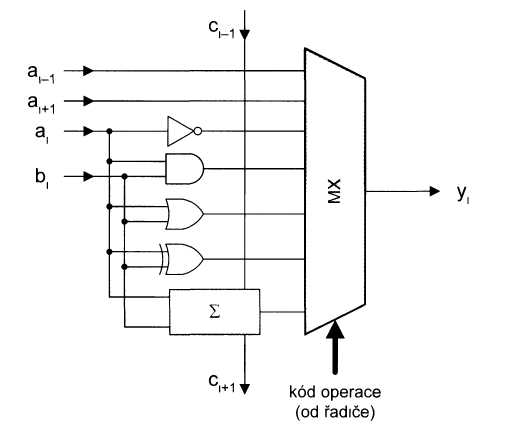
\includegraphics[width=0.7\linewidth]{ALU1bit.png}
        \caption{Část jednoduché aritmeticko-logické jednotky pro 1 bit}
        \label{MIT:fig_ALU1b}
      \end{figure}

       Zřejmě se jedná o ryze kombinační obvody. Rozšířením o \textbf{násobení a dělení} se 
       složitost \texttt{ALU} významně zvětšuje. Násobení dvou slov ve všech bitech současně 
       vyžaduje obvody velmi složité, které mají opodstatnění jen u procesorů s extrémními nároky 
       na rychlost, jako jsou signálové procesory. Druhou krajností je násobení bit po bitu s 
       posuny jednoho operandu -to je příliš pomalé. V běžném případě se volí kompromis a násobička 
       je konstruována na násobení skupiny bitů (půlbyte či byte), takže celé slovo je vynásobeno 
       jen v několika málo krocích, takže příslušné obvody jsou již sekvenční. Totéž platí o 
       operaci dělení.
       
       \textbf{Posuny vlevo a vpravo} o větší počet pozic mohou být prováděny postupně, v několika 
       shodných instrukcích posunu o 1 místo - v některých případech tak však může vzniknout 
       významná časová ztráta a proto některé procesory mají možnost provádět takovéto posuny v 
       jedné instrukci. K tomu je nutná dosažitelnost i vzdálenějších bitů, jak ukazuje obr. 
       \ref{MIT:fig_ALUshift}.
              
      \begin{figure}[ht!] %\ref{MIT:fig_ALUshift}
        \centering
        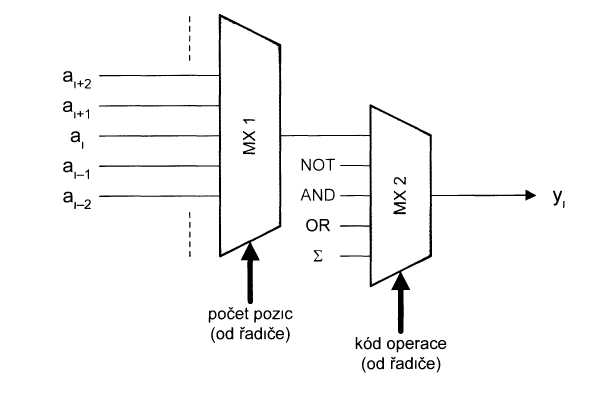
\includegraphics[width=0.7\linewidth]{ALU_shift.png}
        \caption{Obvody pro posun vlevo či vpravo o větší počet kroků}
        \label{MIT:fig_ALUshift}
      \end{figure}    
      
      U mnoha procesorů je \texttt{ALU} doplněna ještě dalšími obvody. Především slouží pro 
      \emph{aritmetické operace  s čísly s plovoucí řádovou čárkou} (čísla typu \textbf{float}). 
      Toto řešení, ačkoliv podstatně zvětšuje složitost \texttt{ALU}, vede k daleko rychlejší 
      činnosti počítače proti běžnějšímu programovému řešení pomocí kni\-hov\-ny aritmetických 
      funkcí v 
      plovoucí čárce. Využívá se zvláště u signálových procesorů.
      
      Existují i jiné doplňky \texttt{ALU}, které vyplývají ze snahy výrobce vylepšit dlouhodobě 
      osvědčený procesor a prodloužit mu tak život. Tak se např. můžeme setkat s jednotkou 
      \textbf{\texttt{MAC}} (z angl. \emph{multiply and accumulate}), která provádí operace 
      násobení dvou čísel, na která ukazují dva adresovací registry, a přičtení výsledku k obsahu 
      speciálního akumulátoru. To je často zapotřebí v úlohách číslicového zpracování signálu. Pro 
      dosažení dostatečného dynamického rozsahu má akumulátor v \texttt{MAC} velmi dlouhé slovo 
      (např. 36 bitů).
      
      \subsubsection{Příznakové bity}
        \emph{Příznakové bity} jsou dalšími výstupy \texttt{ALU}. Ačkoliv jejich počet, označení a 
        význam se může u různých procesorů lišit, některé vlastnosti jsou obecně platné. Některé 
        bity jsou uloženy do příznakového registru, jsou zapamatovány a mohou být použity později. 
        V tomto případě bity vyjadřují výsledek poslední operace, která na ně měla vliv. Zápisový 
        impulz do registru vydává řadič jen v některých instrukcích. U některých procesorů jsou 
        však některé bity vydávány přímo, mimo registr. Pak je jejich stav závislý na okamžité 
        situaci na výstupu akumulátoru. Nejsou tedy zapamatovány. To může být příčinou neúspěchu 
        při nepozorném přepisování programu v assembleru jednoho procesoru do jiného.
        
        Kromě automatického ovlivňování v průběhu instrukce lze do \textbf{registru příznaků 
        \texttt{F}} zasáhnout též přímo (programově) a záměrně tak ovlivnit stav příznakových bitů. 
        U některých procesorů k tomu existují speciální instrukce, u jiných je \texttt{F} přístupný 
        stejně jako datové registry.
        \begin{itemize}\addtolength{\itemsep}{-0.5\baselineskip}
          \item \textbf{Bit \texttt{C}} (též \texttt{CY}) - \emph{přenos} (angl. \emph{carry})  
                \emph{z nejvyššího bitu}. Vždy pamatován. Mění stav při aritmetických operacích, 
                operacích porovnání a některých typech posunů a rotací.
         
          \item \textbf{Bit \texttt{Z}} - \emph{nulovost} (angl. \emph{zero}). U některých      
                procesorů je  zapamatován jako výsledek aritmeticko-logické operace, u jiných se 
                vztahuje na momentální  obsah akumulátoru. Po instrukcích přesunů dat do \texttt{A} 
                tedy v prvém případě není bit \texttt{Z} ovlivněn, ve druhém ano.
        
          \item \textbf{Bit \texttt{S}} - \emph{znaménko čísla} (angl. sign), též \texttt{N} (angl. 
                \emph{negative}). Je nastaven na \texttt{1}, byl-li znaménkový bit výsledku 
                \texttt{1} (tj.  záporné číslo) -jinak je vynulován. U některých procesorů je 
                zapamatován, u jiných není vůbec realizován a test znaménka je nahrazen instrukcí 
                \emph{„testuj bit..."}.
        
          \item \textbf{Bit \texttt{V}} (též \texttt{OV}) - \emph{přetečení} (angl.   
                \emph{overflow}). Vždy pamatován. Mění stav při přetečení čísla se znaménkem 
                (nejvyšší bit slova) po operaci součtu, rozdílu, obrácení znaménka, násobení a 
                dělení. Operandy i výsledek se předpokládají ve dvojkovém doplňku. Kladný výsledek 
                nemůže být větší než \texttt{7FF...F}, vyšší hodnota by způsobila změnu 
                znaménkového bitu. Záporný výsledek nemůže být menší než \texttt{800...0} a 
                nižší hodnota by opět způsobila změnu znaménkového bitu. U operace dělení je takto 
                zpravidla signalizováno dělení nulou.
        
          \item \textbf{Bit \texttt{H}} (též \texttt{AC}) - \emph{poloviční přenos} (angl.  
                \emph{half-carry}) nebo \emph{pomocný přenos} (angl. \emph{auxiliary carry}). Vždy 
                pamatován. Jedná se o přenos z bitu \texttt{D3} do \texttt{D4} při operaci součtu. 
                Je využíván následnou instrukcí dekadické korekce akumulátoru, pokud sčítaná čísla 
                byla v \texttt{BCD} kódu.
        
          \item \textbf{Bit \texttt{P}} - \emph{parita} (angl. \emph{parity}) vyjadřuje paritu     
                výsledku (počet jedniček). Při \textbf{liché paritě} je \texttt{P = 1} při lichém 
                počtu jedniček, u \textbf{sudé parity} je \texttt{P = 1} při sudém počtu jedniček. 
                Je třeba zjistit, jakou paritu bit vyjadřuje. Paritní bit mají jen některé 
                procesory. Kontrola paritou slouží hlavně jako diagnostický prostředek, je však 
                značně nespolehlivá. 
        \end{itemize}        
        
        Uvedené příznakové bity mohou být doplněny ještě dalšími, méně běžnými, podle architektury procesoru.
      
      \subsubsection{Další využití ALU}
        V mnoha instrukcích je adresa v datové paměti tvořena jako součet adresové části instrukce 
        a obsahu dalšího registru (např. \textbf{indexová adresace}). Dále adresa následující 
        instrukce v programové paměti je dána jako adresa současně prováděné instrukce plus délka 
        této instrukce - při proměnlivé délce instrukcí tedy zřejmě nestačí jen prostá inkrementace 
        \texttt{PC}. Existují též instrukce s relativní adresací (\textbf{relativní skoky}), kdy 
        adresa následující instrukce je tvořena jako momentální obsah \texttt{PC} plus adresová 
        část skokové instrukce. Je tedy zřejmé, že pro adresaci v datové paměti i v programové 
        paměti je nutné provádět operaci součtu dvou čísel. K tomu účelu lze využít již existující 
        \texttt{ALU}. Je to běžně používané řešení, které má výhodu obvodové úspornosti. Nevýhodou 
        je ale prodloužení instrukčního cyklu, neboť jedna jediná \texttt{ALU} nemůže  všechny výše 
        uvedené operace (a navíc ještě aritmetické a logické operace v příslušných instrukcích) 
        provádět \emph{současně}.
        
        Při vyšších nárocích na rychlost jsou proto procesory vybaveny několika sčítačkami vedle 
        univerzální \texttt{ALU}. Např. jedna sčítačka je spojena s \texttt{PC}, druhá vytváří 
        adresu pro datovou paměť.
        
        V algoritmech číslicového zpracování signálu (i některých dalších) je třeba opakovaně 
        zpracovávat pole dat. Adresa v datové paměti se v nejjednodušším případě postupně 
        inkrementuje (zvyšuje) o jedničku, ale častěji ve větších krocích a v aritmetice 
        \texttt{modulo M}. Při extrémních nárocích na rychlost provádění těchto algoritmů je 
        procesor (\emph{signálový procesor}) vybaven speciální adresovací jednotkou - 
        \texttt{generátorem adres}. Ta přebírá úlohu automatické generace adres, kterou by jinak 
        bylo nutno řešit programově a tudíž mnohem pomaleji.
      
    \subsection{Prostředky pro zrychlení činnosti procesoru}
      První a samozřejmou možností je \emph{zvyšování hodinového kmitočtu}. Závisí na pokrocích v 
      technologii výroby integrovaných obvodů. V tomto směru se zatím stále postupuje. Druhou 
      možností je \emph{zvětšování délky slova}. Ve srovnání s \texttt{ALU} s osmibitovými daty 
      bude \texttt{ALU} se šestnáctibitovými daty znamenat dvojnásobnou rychlost práce (měřeno v 
      počtu bitů za sekundu), u 32bitových a 64bitových slov je zrychlení samozřejmě ještě větší. 
      Zvětšování délky slova ale znamená vyšší cenu pouzder integrovaných obvodů (větší počet 
      vývodů datové sběrnice), vyšší složitost a vyšší cenu plošného spoje. Třetí možností jsou 
      zásahy do \emph{architektury procesoru}.
      
      Jednoduchá architektura, tak jak ji ilustruje obr. \ref{MIT:fig_procesor}, bude zpracovávat 
      instrukci \emph{„sečti obsah proměnné ..., indexová adresace, s obsahem akumulátoru"}, 
      přičemž se předpokládá, že výsledek zůstává v akumulátoru. Posloupnost činností během 
      instrukčního cyklu ukazuje obr. \ref{MIT:fig_pipeline01}. Program je v tomto případě uložen v 
      paměti \texttt{ROM}, data v paměti \texttt{RAM}. Procesor je vybaven index-registrem a adresa 
      pro \texttt{RAM} je generována jako součet adresové části instrukce a obsahu index-registru.
      
      \begin{figure}[ht!] %\ref{MIT:fig_pipeline01}
        \centering
        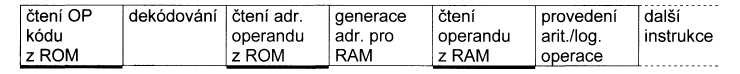
\includegraphics[width=0.9\linewidth]{pipeline01.jpg}
        \caption{Posloupnost činností jednoduchého procesoru}
        \label{MIT:fig_pipeline01}
      \end{figure}     
      
      Využití vnějších sběrnic je vyznačeno tlustou čárou. Na obr. \ref{MIT:fig_pipeline01} se 
      pravidelně střídá činnost s nečinností, v jiných instrukcích však může obraz vypadat jinak. 
      Jedině čtení operačního kódu a jeho dekódování se shoduje u všech instrukcí, další činnost a 
      tedy i využití sběrnic se může lišit podle typu instrukce. Z toho je zřejmé, že:
      \begin{itemize}\addtolength{\itemsep}{-0.5\baselineskip}
        \item Vnější sběrnice jsou využity jen po část instrukčního cyklu, v podstatě nepravidelně.
        \item Během čtení operačního kódu a jeho dekódování je nečinná \texttt{ALU}, naopak během  
              provádění  instrukce nepracuje dekodér instrukcí. Zrychlení činnosti je možné tak, že 
              rozdělíme instrukční cyklus na dvě fáze: \textbf{fázi čtení + dekódování}, a 
              \textbf{fázi provádění}. Umožníme tak čtení a dekódování další instrukce již během 
              provádění instrukce předcházející, jak ukazuje obr. \ref{MIT:fig_pipeline02}.
      \end{itemize}        
      
      \begin{figure}[ht!] %\ref{MIT:fig_pipeline02}
        \centering
        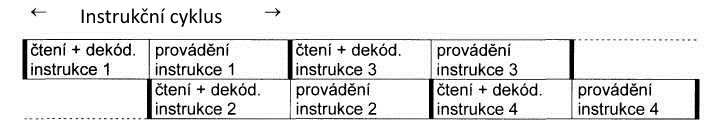
\includegraphics[width=0.9\linewidth]{pipeline02.jpg}
        \caption{Překrývání dvou fází instrukcí}
        \label{MIT:fig_pipeline02}
      \end{figure}     

      V ideálním případě se tak zřejmě dosáhne dvojnásobného zrychlení instrukčního cyklu. Procesor 
      v každém okamžiku pracuje se dvěma instrukcemi. Je však nutné zajistit oddělení obou stupňů 
      oddělovacími registry - zápisem do registru se výsledek činnosti prvého stupně přesune do 
      druhého stupně, a prvý stupeň se tak uvolní pro novou instrukci. Zcela zřejmě se jedná o 
      \emph{zřetězenou strukturu} - \textbf{„pipeline"}, známou z teorie číslicových systémů. 
      Princip zřetězení lze aplikovat ještě dále a vyrovnávacími registry rozdělit procesor na 
      větší počet úseků, čímž se efekt zřetězené struktury projeví ještě markantněji. Procesor tak 
      zpracovává vždy několik instrukcí, vzájemně posunutých. Rozdělení na dílčí úseky může vypadat 
      následovně:
      \begin{itemize}\addtolength{\itemsep}{-0.5\baselineskip}
        \item Čtení OP kódu z programové paměti.
        \item Dekódování instrukce.
        \item Výpočet adres operandů.
        \item Čtení operandů z datové paměti.
        \item Činnost \texttt{ALU}, která sama může být zřetězena. Zvláště je-li vybavena pro  
              operace v pohyblivé čárce, které jsou vždy prováděny v několika krocích.
        \item Zápis výsledků do datové paměti.
      \end{itemize}
      
      Další úpravou je \emph{rozdělení procesoru na dvě samostatné jednotky} - instrukční jednotku 
      a výkonnou jednotku. \textbf{Instrukční jednotka} (angl. \emph{Bus Interface Unit, BIU}) čte 
      instrukce z programové paměti. Instrukce dekóduje a čte operandy z datové paměti. Používá k 
      tomu svůj vlastní generátor adres. Dekódované instrukce (výstup z instrukčního dekodéru) a 
      operandy předává výkonné jednotce. \textbf{Výkonná jednotka} (angl. \emph{Execution Unit, 
      EU}) má svůj řadič a \texttt{ALU}. Pokud výsledek operace \texttt{EU} má být uložen do datové 
      paměti, děje se tak opět prostřednictvím \texttt{BIU}. 
      
      Mezi \texttt{BIU} a \texttt{EU} je vložena paměť typu \texttt{FIFO} (\emph{paměť fronty}), 
      která vyrovnává krátkodobé rozdíly mezi rychlostmi práce obou jednotek. V této vyrovnávací 
      paměti je uloženo několik dekódovaných instrukcí včetně operandů. Díky tomu nemusí jedna 
      jednotka čekat na druhou. \texttt{BIU} plně využívá možnosti vnějších sběrnic a zaplňuje 
      \texttt{FIFO} v případě, že \texttt{EU} právě pracuje na instrukcích s dlouhou dobou 
      zpracování (např. násobení, dělení). \texttt{EU} má ve \texttt{FIFO} rezervu několika 
      instrukcí v případě, že právě prováděné instrukce potřebují jen krátkou dobu na zpracování 
      (např. vnitřní přesuny mezi registry) a \texttt{BIU} nemůže dodávat nové instrukce tak 
      rychle. Vnější sběrnicové cykly neodpovídají právě vykonávané instrukci v \texttt{EU}. Pro 
      účely ladění programů může však být tato informace o tom, která instrukce je právě 
      vykonávána, nezbytná. Některé procesory proto mají zvláštní výstupy, na kterých vydávají 
      informaci o stavu zaplnění \texttt{FIFO}.
      
      Skutečnost, že zřetězený procesor pracuje na několika instrukcích současně, však přináší i 
      komplikace. Zřetězená struktura představuje zrychlení jen při plynulém dodávání dat na vstup. 
      Narušení plynulosti nastává v instrukci skoků nebo volání podprogramů, kdy za touto instrukcí 
      jsou v řetězci (a ve \texttt{FIFO}) již načteny a případně částečně zpracovány další 
      instrukce, které bezprostředně následovaly v programové paměti. Provedením skoku se dostáváme 
      do jiné oblasti programové paměti, kde následují samozřejmě zcela jiné instrukce. 
      \texttt{FIFO} je nutno z \texttt{BIU} naplnit novými instrukcemi. Zvláště obtížná je situace 
      u podmíněných skoků, kdy nelze předvídat, kterou ze dvou větví bude program pokračovat. 
      Existují sice hardwarové i softwarové prostředky, kterými lze v některých případech frontu 
      instrukcí zachovat (zdvojené \texttt{FIFO}, každé je plněno jednou alternativní sekvencí 
      instrukcí a k přepnutí dojde po vyhodnocení podmínek skoku) a rozpracované instrukce dokončit 
      (metoda \textbf{„zpožděného skoku"}), ale obecně platí, že časté skoky a volání snižují 
      účinnost zřetězeného zpracování.
      
      Ke konfliktům může docházet i v datech. Je to v případě, že instrukce \texttt{1} je právě 
      dokončována a její výsledek má být uložen do paměti. Současně je ale načítán operand 
      instrukce \texttt{2}, který je shodou okolností na stejné adrese v paměti. Při sekvenčním 
      zpracování instrukcí, kdy data, zpracovaná instrukcí \texttt{1} a uložená do paměti, jsou v 
      instrukci \texttt{2} z paměti přečtena a dále zpracována, nevzniká žádný problém, ale u 
      zřetězeného zpracování ano. Přečtení dat v instrukci \texttt{2} (což následuje ihned po 
      přečtení \texttt{OP} kódu) totiž může předběhnout uložení dat do paměti v instrukci 
      \texttt{1}. Konflikt lze řešit na úrovni software při překladu - překladač mezi dvě 
      konfliktní instrukce vloží potřebný počet prázdných instrukcí (\texttt{NOP}), čímž vznikne 
      potřebný časový odstup. Lepší řešení spočívá v hardwarové úpravě procesoru o obvody, 
      detekující v instrukčním dekodéru konfliktní skupiny instrukcí (na základně shodnosti adres 
      operandů). Načítání operandů pro instrukci \ \texttt{2} je automaticky zpožděno až za okamžik 
      zápisu výsledku instrukce \texttt{1}.

    \subsection{Procesory typu RISC a CISC}  
      Procesory typu \texttt{CISC} jsou základem počítačů \texttt{CISC} (angl. \emph{Complex 
      Instruction Set Computer}) - počítačů se složitým souborem instrukcí. Procesory typu 
      \texttt{RISC} jsou základem počítačů \texttt{RISC} (angl. \emph{Reduced Instruction Set 
      Computer}) - počítačů se zjednodušeným souborem instrukcí. Soubory instrukcí moderních 
      procesorů jsou velmi rozsáhlé a mnohé z nich realizují operace tak složité, že by je bylo 
      možné nahradit celým úsekem programu, sestaveného z jednoduchých instrukcí. Často jsou tyto 
      instrukce „šity na míru" pro snadnou kompilaci z jazyka \texttt{C}. Důsledkem je ale velmi 
      složitý řadič procesoru, řešený vždy jako mikroprogramový automat. Celý procesor 
      je pomalejší.
      
      Naopak u procesoru \texttt{RISC} je soubor instrukcí zúžen na pečlivě vybrané jednoduché, 
      často používané instrukce. Tím je usnadněna účinná optimalizace obvodů procesoru s cílem 
      maximálního zrychlení činnosti. Řadič je konstruován jako klasický sekvenční obvod s důrazem 
      na maximální rychlost. Program, sestavený z jednoduchých instrukcí \texttt{RISC}, je 
      samozřejmě delší než program, sestavený z instrukcí \texttt{CISC} - celková doba na jeho 
      provedení je však kratší vzhledem k rychlosti provádění jednoduchých instrukcí. Pro účinnost 
      této metody je však nutné pozměnit architekturu procesoru.
      
      Procesory RISC se vyznačují těmito vlastnostmi:
      \begin{itemize}\addtolength{\itemsep}{-0.5\baselineskip}
        \item Instrukce mají jednotnou délku (v počtu byte) a jsou prováděny zpravidla v jednom   
              strojním cyklu. Tím je zvýšena účinnost zřetězeného zpracování. Výjimku tvoří 
              instrukce, pracující s vnější datovou pamětí.        
        \item Typické jsou instrukce tříoperandové - např. \emph{„sečti obsah registru 1 s obsahem  
              registru 2 a výsledek ulož do registru 3"}. Adresa registrů však nesmí být dlouhá, 
              aby se neprodlužovala instrukce.
        \item Většina instrukcí pracuje s vnitřními registry. Ty jsou dosažitelné mnohem rychleji,  
              než vnější paměť. K adresování registrů postačí malý počet bitů adresy, proto i 
              tříoperandové instrukce mohou být krátké.        
        \item Výsledek operace \texttt{ALU} není ukládán do akumulátoru, ale do libovolného    
              vnitřního registru. Tím odpadají časté přesuny dat z a do akumulátoru.
        \item Je běžné přepínání bank registrů.        
        \item Důsledně je uplatněno zřetězené zpracování.        
        \item Kompilátor z vyššího jazyka je složitý, optimalizuje rychlost a může za tím účelem i  
              měnit pořadí instrukcí.       
      \end{itemize}
    
    \subsection{Základní typy instrukcí}
      \subsubsection{Adresace v instrukcích}
        Adresa slouží k určení \textbf{zdroje} dat (angl. \emph{source address}) nebo cíle dat 
        (angl. \emph{destination address}). Nejčastější způsoby adresace jsou následující:
        \begin{itemize}\addtolength{\itemsep}{-0.5\baselineskip}
          \item \textbf{Bezprostřední data} (angl. \emph{immediate}). Data jsou obsažena již v  
                instrukci, která v tomto případě obsahuje datovou část. Tento způsob adresace je 
                uváděn jen pro úplnost, žádná adresa vlastně není zapotřebí.
          \item \textbf{Přímá adresa} (angl. \emph{direct}). Adresa je obsažena v instrukci, která  
                v tomto případě obsahuje adresovou část.
          \item \textbf{Nepřímá adresa} (angl. \emph{indirect}). V instrukci není uvedena adresa,  
                ale zdroj adresy. Během provádění instrukce je tento zdroj přečten a tak je teprve 
                získána adresa. Zdrojem adresy může být buď některý z vnitřních registrů procesoru, 
                nebo paměť. Jedná se tedy o nepřímou adresaci prostřednictvím registru nebo 
                prostřednictvím paměti. Při nepřímé adresaci registrem je definice registru 
                součástí instrukčního kódu (počet možných registrů je malý), takže instrukce je 
                krátká. Rovněž získání adresy proběhne rychle, neboť registr je součástí procesoru 
                a může rovnou sloužit jako zdroj adresy. Naopak při nepřímé adresaci                
                prostřednictvím paměti musí být v instrukci uvedena nepřímá adresa v plné délce. 
                Provádění instrukce je pomalejší, přibývá jeden cyklus (čtení adresy z paměti). 
                Výhodou však je to, že počet možných zdrojů nepřímé adresy je prakticky neomezený, 
                na rozdíl od počtu registrů při prvém způsobu. Nepřímá adresa je často využívána ve 
                vyšších programovacích jazycích (typ \emph{pointery C}).
          \item \textbf{Relativní adresa} (angl. \emph{relative}). Instrukce obsahuje adresovou  
                část, tzv. offset, jejíž obsah se přičte k obsahu čítače instrukcí. Využívá se 
                nikoliv ke čtení nebo zápisu dat, ale k získání adresy následující instrukce v 
                některých instrukcích skoků nebo smyček typu „skoč o offset dále od momentální 
                polohy čítače instrukcí. Offset je vždy chápán jako číslo se znaménkem, takže skoky 
                v programu jsou možné vpřed i vzad. Offset bývá kratší než přímá adresa (typicky 1 
                slabika), takže relativní adresace je úsporná z hlediska délky instrukce. 
                Vzdálenost v programu, kterou lze skokem překlenout, je však omezená.
          \item \textbf{Indexová adresa} (angl. \emph{indexed}). K adresové části instrukce je  
                přičten obsah indexregistru a tento součet je teprve použit jako adresa pro data 
                (přímá indexová adresace), nebo jako adresa pro zdroj adresy (nepřímá indexová 
                adresace). Indexregistry jsou nejčastěji dva a jsou součástí procesoru. Indexová 
                adresace je výhodná pro práci s tabulkami (pole v jazyce \texttt{C}).
        \end{itemize}
        
        Pro realizaci některých algoritmů (např. číslicového zpracování signálů) je nutné mnohokrát 
        probíhat programovou smyčkou a zpracovávat data s postupně se měnícími adresami. Obdobně je 
        nutné postupně zvyšovat adresy při přesunech bloků dat z jedné oblasti paměti do druhé. V 
        těchto případech se využije možnost \textbf{autoinkrementace} či autodekrementace adresy. 
        Adresace je přitom \emph{nepřímá} prostřednictvím registru. Na konci provádění instrukce je 
        automaticky inkrementován (dekrementován) obsah \emph{adresovacího registru}. Některé 
        instrukce umožňují i inkrementaci (dekrementaci) dvou registrů, takže jsou automaticky 
        posunovány ukazatele na adresu zdroje a cíle při přesunech bloků, nebo ukazatel do pole 
        vzorků a ukazatel do pole koeficientů (typické např. pro \emph{diskrétní Fourierovu 
        transformaci}). U některých procesorů (signálových procesorů) může být velikost inkrementu 
        (dekrementu) volitelná a adresu lze generovat v aritmetice „modulo M". To je zvláště 
        důležité pro rychlé provádění algoritmů číslicového zpracování signálů. Absolutní adresa, 
        vypočítaná v průběhu instrukce z adresy uložené v adresové části instrukce, se nazývá 
        \textbf{efektivní adresa}.
        
        Všechny výše uvedené způsoby adresace nejsou samozřejmě dostupné u každého procesoru. 
        Dokonalejší (zvláště 16 a vícebitové) procesory je však obsahují zcela běžně.
        
        Pro některé programové úlohy je nutné znát \textbf{pořadí ukládání} jednotlivých slabik v 
        paměti (Endianita, angl. \emph{„Byte Order"}). Týká se adres a dlouhých proměnných. 
        Existují dvě možnosti: nejnižší slabika na nejnižší adrese (pořadí \textbf{LO-HI}, tzv. 
        \emph{„Little Endian"}), a nejvyšší slabika na nejnižší adrese (pořadí \textbf{HI-LO}, tzv, 
        \emph{„Big Endian"}). Pořadí se liší i u různých procesorů téhož výrobce a je to důležitá 
        informace, kterou je nutno v dokumentaci někdy pracně hledat. Pořadí bitů ve slabice je 
        vždy takové, že nejvyšší bit ve slabice \texttt{MSB} (angl. \emph{Most Significant Bit}) je 
        na pozici \texttt{D7}, nejnižší bit \texttt{LSB} (angl. \texttt{Least Significant Bit}) je 
        na pozici Do.
        
      \subsection{Typy instrukcí a jejich provádění}
        Soubory instrukcí různých procesorů se sice vzájemně liší, přesto však lze nalézt společné 
        vlastnosti, podle kterých mohou instrukce být zařazeny do několika hlavních skupin. Pro 
        programování v assembleru je nutné znát přesnou syntaxi jednotlivých instrukcí i činnost 
        počítače v nich. Detaily lze nalézt ve firemní literatuře. I \emph{symbolické názvy} 
        instrukcí, též „mnemotechnické instrukce" (angl. \emph{mnemonic code}) se liší u různých 
        výrobců. V této kapitole nebude popisován soubor instrukcí žádného konkrétního typu 
        procesoru, nýbrž bude podán přehled základních instrukcí. Instrukce zde uváděné jsou 
        fiktivní, i když bylo snahou vybrat názvy blízké názvům skutečným a nejčastějším, či 
        nejvýstižnějším.
        
        \textbf{Operandy} v instrukcích jsou v dalším textu značeny následovně:
        \begin{itemize}\addtolength{\itemsep}{-0.5\baselineskip}
          \item \texttt{x, y}: přímá adresa, nepřímá adresa prostřednictvím paměti, nepřímá  
                adresa prostřednictvím registru, označení registru, přímý operand;
          \item \texttt{reladdr}: relativní adresa (zpravidla krátká);
          \item \texttt{r}: označení registru;
          \item \texttt{inaddr}: adresa vstupního obvodu;
          \item \texttt{outaddr}: adresa výstupního obvodu.          
        \end{itemize}
        
        Uvedené značení operandů je velmi hrubé a vhodné jen pro popis typů instrukcí. Pro zjištění 
        všech možností a omezení u konkrétního typu procesoru je nutné se seznámit s dokumentací 
        výrobce.
        
        \subsubsection{Instrukce přesunů dat}
          Přesuny jsou možné mezi vnitřními registry procesoru, mezi pamětí a vnitřním registrem a 
          mezi dvěma adresami v paměti. Obsah cíle dat se přepíše novými daty, obsah zdroje dat se 
          nemění.
        
          \emph{Typické instrukce přesunů:}
            \begin{lstlisting}[gobble=10]
              MOV x,y   ;univerzalni
              LDR x     ;mem -> reg
              STR x     ;reg -> mem
              TRL r1,r2 ;reg -> reg
              EX  r1,r2 ;reg <-> reg
            \end{lstlisting}
      
          Směr přenosu je dán konvencí při psaní instrukcí, tzv. „směr šipky" - zpravidla na prvém 
          místě je označení cíle dat a na druhém místě zdroje dat (ale pozor, u některých procesorů 
          může u některých instrukcí být směr opačný-pečlivé prostudování konkrétního seznamu 
          instrukcí je vždy nutné).
          
        \subsubsection{Instrukce aritmeticko-logické}           
          Jsou prováděny v akumulátoru, kde je pak rovněž uložen výsledek. Pokud instrukce pracuje 
          se dvěma operandy, musí zpravidla být jeden již předem uložen v akumulátoru a druhý je 
          určen v instrukci. Některé procesory však umožňují pracovat s operandy v registrech 
          zápisníkové paměti a směrovat výsledek rovněž do nich, nebo do paměti. To může významně 
          zrychlit program, neboť je tak odstraněna  nutnost častého přesunování operandů mezi 
          akumulátorem a registry či pamětí.
         
          \emph{Typické aritmetické instrukce:}
          \begin{lstlisting}[gobble=10]
            ADD x    ;pricte operand k akumulatoru
            ADDC x   ;totez, navic pricte bit C
            SUB x    ;odecte operand od akumulatoru
            SUBB x   ;totez, navic odecte bit C 
                     ;(zaporny prenos, "borrow")
          \end{lstlisting}
         
          Jeden operand je předem uložen v akumulátoru. Instrukce se započítáním přenosu jsou 
          využívány hlavně při práci s dlouhými proměnnými o větším počtu slabik, kdy součet 
          (rozdíl) je prováděn postupně (po slabikách). Některé procesory mají pro jednoduchost jen 
          instrukce \texttt{ADDC} a \texttt{SUBB}, takže při operacích bez započítání přenosu se 
          musí předem vynulovat bit \texttt{C}.
         
          \begin{lstlisting}[gobble=10]
            NEG x  ;obraceni znamenka 
                   ;(negace vsech bitu +1)
            INC x  ;inkrementace (+ 1)
            DEC x  ;dekrementace (- 1)
            CLR x  ;vynulovani
            DAA    ;dekadicka korekce akumulatoru
          \end{lstlisting}
         
          Instrukce \texttt{DAA} se používá po předcházející operaci součtu dvou čísel v 
          \textbf{BCD kódu} (\emph{Binary Coded Decimal}). Každá dekadická číslice je kódována 
          čtveřicí bitů, \emph{„půlbyte"} (angl. \emph{nibble}), takže v jedné slabice jsou dvě 
          dekadické číslice (tzv. \emph{kompaktní tvar BCD}). V binárním kódu jsou čtveřice bitů 
          vyjádřeny jako hexadecimální (šestnáctkové) číslice s hodnotami \texttt{0...9, A, B, C, 
          D, E, F}. Binární sčítačka ovšem sčítá \texttt{BCD} čísla jako by byla binární a tím 
          vzniká chyba. Tu je třeba korigovat. Pokud součet v rámci čtveřice bitů nepřesáhne 
          \texttt{9}, je vše v pořádku. Je-li součet v rozsahu \texttt{10} až \texttt{15} 
          (\texttt{AH} až \texttt{FH}), mělo by dojít k přenosu do vyššího dekadického řádu (tj. do 
          vyšší čtveřice bitů). U binárních čísel však ještě k přenosu nedojde, rozsah čtveřice 
          bitů je \texttt{0...15 (0...FH)}. Až při výsledku \texttt{16} a výše dojde k přenosu, což 
          je signalizováno nastavením příznakového bitu \texttt{H} (\emph{half-carry}). Korekce je 
          provedena přičtením čísla \texttt{6} kdykoliv součet v rámci dolní čtveřice bitů přesáhne 
          \texttt{9} nebo když příznakový bit  \texttt{H = 1}. Totéž se provede v horní čtveřici 
          bitů, jen místo bitu \texttt{H} se pracuje s bitem \texttt{C}. Některé procesory mají 
          ještě instrukci pro korekci po rozdílu dvou \texttt{BCD} čísel. Průběh je obdobný, šestka 
          se však odečítá.
         
          \begin{lstlisting}[gobble=10]
            MUL   ;nasobeni cisel bez znamenka
            MULS  ;nasobeni cisel se znamenky
          \end{lstlisting}
           
          U násobení bývá předem přesunut jeden operand do akumulátoru a druhý do jiného registru, 
          pro tuto instrukci pevně předurčeného. Výsledek (dvojnásobné délky) je pak v obou těchto 
          registrech.
          
          \begin{lstlisting}[gobble=10]
            MAC x ;soucin a akumulace 
                  ;(angl. multiply and accumulate), 
                  ;vysledek akumuluj na adrese x
          \end{lstlisting}
         
          Pro mnoho algoritmů číslicového zpracování dat, statistických výpočtů apod. je nutné 
          opakovaně násobit dvě čísla (např. vzorky signálu a váhové koeficienty z tabulky) a dílčí 
          součiny stále přičítat. Přitom nároky na rychlost zpracování bývají značné. Novější 
          procesory proto byly vybaveny instrukcí \texttt{MAC}. Akumulátor v tomto případě bývá 
          jiný než je registr \texttt{A} v \texttt{ALU} - je to buď další, specializovaný 
          akumulátor, dvojice registrů zápisníkové paměti, nebo proměnná dvojnásobné délky v 
          paměti. Dvojnásobná délka je nutná k zabránění přetečení při mnohonásobném opakování 
          \texttt{MAC}. Ani dvojnásobná délka akumulátoru však není mnohdy dostatečná a 
          specializovaný akumulátor má např. 36 bitů (rezerva 4 bity nad 4 slabiky). Adresování v 
          instrukci \texttt{MAC} je typicky pomocí indexregistrů (musí se měnit adresy obou 
          operandů) nebo jiných registrů, předurčených pro tuto operaci. Výsledek je u některých 
          procesorů směrován jedině do   speciálního akumulátoru a pak \texttt{MAC} nemá adresovou 
          část. Důležitá pro rychlé opakování \texttt{MAC} ve smyčce je tvorba nových adres 
          operandů. Pokud nejsou adresy vytvářeny automaticky, je jejich programová tvorba 
          zpravidla příliš pomalá a účinnost \texttt{MAC} je podstatně snížena.
         
          \begin{lstlisting}[gobble=10]
            DIV  ;deleni cisel bez znamenka
            DIVS ;deleni cisel se znamenky
          \end{lstlisting}
       
          U dělení bývá umístěn dělenec v akumulátoru, dělitel v jiném registru, pro tuto instrukci 
          pevně předurčeném, výsledný celočíselný podíl zůstává v akumulátoru, a zbytek po dělení v 
          registru, předurčeném pro dělitele.
      
          \emph{Typické logické instrukce:}
            \begin{lstlisting}[gobble=10]
              AND x ;log. soucin operandu s akumulatorem
              OR x  ;log. soucet operandu s akumulatorem
              XOR x ;exkluzivni log. soucet 
                    ;operandu s akumulatorem
              NOT x ;tez COM - negace (komplement) 
                    ;vsech bitu operandu
            \end{lstlisting}
      
          Mezi aritmeticko-logické instrukce se zpravidla počítají i instrukce porovnání. Vždy se 
          provede odečtení obou operandů. Výsledek však není nikam ukládán, ale projeví se jen 
          nastavením patřičných příznakových bitů, podle kterých lze pak větvit program.
       
          \begin{lstlisting}[gobble=10]
            CMP x,y  ;porovnani, druhy operand se 
                     ;odecte od prveho, ovlivni
                     ;priznakove bity C, Z, S, V.
          \end{lstlisting}
       
          U některých procesorů je první operand implicitně v akumulátoru, pak má instrukce tvar
       
          \begin{lstlisting}[gobble=10]
            CMP x    ;porovnani, operand se odecte od 
                     ;obsahu akumulatoru, ovlivni 
                     ;priznakove bity C, Z, S, V
          \end{lstlisting}

        \subsubsection{Instrukce pro logické operace s jednotlivými bity}      
          Operace s jednotlivými bity jsou velmi užitečné zvláště v úlohách řízení. Jako 
          jednobitové vstupní proměnné vystupují např. signály ze spínačů, výstupními proměnnými 
          jsou signály pro ovládání akčních členů (zapnout-vypnout), apod. Též jsou intenzívně 
          využívány při ovládání periferních obvodů počítače. Adresování bitů je možné dvojím 
          způsobem: některé procesory mají malou oblast paměti adresovatelnou po jednotlivých 
          bitech, jiné umožňují zadat adresu ve dvou složkách jako \texttt{adresa\_slova} \(\cdot\) 
          \texttt{pořadí\_bitu}. Tak v prvém případě např. \texttt{bitaddr = 19} (dekadicky) 
          odpovídá ve druhém případě \texttt{bitaddr = 2.3}:

          \begin{table}[ht!]
            \begin{tabular*}{0.73\textwidth}{llllllllll}
                          & pořadí bitu: & 7  & 6  & 5  & 4  & \textbf{3}  & 2  & 1  & 0  \\ \cline{1-10}
              addr.       & 0 bitaddr    & 7  & 6  & 5  & 4  & 3           & 2  & 1  & 0  \\
              byte:       & 1            & 15 & 14 & 13 & 12 & 11          & 10 & 9  & 8  \\
                          & \textbf{2}   & 23 & 22 & 21 & 20 & \textbf{19} & 18 & 17 & 16 \\
                          & 3            & 31 & 30 & 29 & 28 & 27          & 26 & 25 & 24 \\
              & 4 & \multicolumn{8}{c}{...........................................................} \\
            \end{tabular*}
            \caption*{ }
          \end{table}

          \begin{lstlisting}[gobble=10]
            BSET bitaddr              ;nastaveni bitu na 1
            BCLR bitaddr              ;vynulovani bitu
            BCPL bitaddr              ;negace bitu
            BMOV bitaddr1,bitaddr2    ;presun bitu
            BAND bitaddr1,bitaddr2    ;log. soucin 2 bitu
            BOR  bitaddr1,bitaddr2    ;log. soucet 2 bitu 
            BXOR bitaddr1,bitaddr2    ;exkluzivni log. 
                                      ;soucet 2 bitu
            BCMP bitaddr1,bitaddr2    ;porovnani 2 bitu
          \end{lstlisting}
          
          U některých procesorů jsou možnosti výběru operandů omezeny - jedním operandem je pak 
          vždy příznakový bit \texttt{C}, výsledek je opět v \texttt{C}.
          
        \subsubsection{Instrukce posunů a rotací}          
          Všechny bity operandu jsou posunuty vlevo či vpravo o počet míst, která jsou dána v 
          instrukci. U některých procesorů však tento parametr neexistuje a posun je vždy o jedno 
          místo.
          \begin{lstlisting}[gobble=10]
            SHL  x,n ;log. posun vlevo  o n mist, 
                     ;nejvyssi bit presunut do
                     ;priznakoveho bitu C, 
                     ;nejnizsi bit vynulovan
            SHR  x,n ;logicky posun vpravo o n mist, 
            ASHR x,n ;aritmeticky posun vpravo o n mist, 
                     ;nejvyssi bit se ale nemeni
          \end{lstlisting}

          \begin{figure}[ht!]
            \centering
            \begin{tabular}{cc}
              \subfloat[SHL ]{\label{fig_MIT:SHL}
                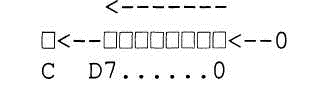
\includegraphics[width=0.45\linewidth]{pinker_SHL.png}}              &
              \subfloat[SHR]{\label{fig_MIT:SHR}
                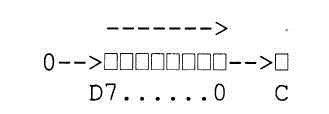
\includegraphics[width=0.45\linewidth]{pinker_SHR.png}}              \\
              \subfloat[ASHR]{\label{fig_MIT:ASHR}
                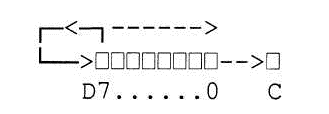
\includegraphics[width=0.45\linewidth]{pinker_ASHR.png}}             &  \\ 
            \end{tabular}
            \caption{Instrukce posunů}
          \end{figure}
         
          Při aritmetickém posunu je operandem číslo se znaménkem, nejvyšší bit je znaménkový. 
          Zůstává zachován a jeho hodnota se šíří doprava (nuly u kladného čísla, jedničky u 
          záporného). Kdyby se číslo se znaménkem podrobilo logickému posunu vpravo, byl by 
          výsledek vždy kladný (nula do nejvyššího bitu), což by u záporného čísla bylo špatně.

          \begin{lstlisting}[gobble=10]
            ROL x ;rotace vlevo, nejvyssi bit presunut 
                  ;do nejnizsiho bitu a soucasne
                  ;do priznakoveho bitu C
            ROR x ;rotace vpravo, nejnizsi bit presunut 
                  ;do nejvyssiho bitu a soucasne
                  ;do priznakoveho bitu C
            RCL x ;rotace vlevo pres priznakovy bit C
            RCR x ;rotace vpravo pres priznakovy bit C
          \end{lstlisting}
          
          \begin{figure}[ht!]
            \centering
            \begin{tabular}{cc}
              \subfloat[ROL]{\label{fig_MIT:ROL}
                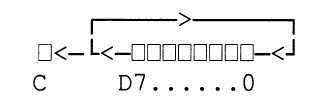
\includegraphics[width=0.45\linewidth]{pinker_ROL.png}}              &
              \subfloat[ROR]{\label{fig_MIT:ROR}
                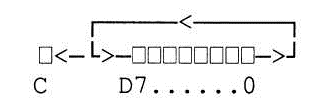
\includegraphics[width=0.45\linewidth]{pinker_ROR.png}}              \\
              \subfloat[RCL]{\label{fig_MIT:RCL}
                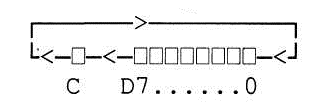
\includegraphics[width=0.45\linewidth]{pinker_RCL.png}}              &
              \subfloat[RCR]{\label{fig_MIT:RCR}
                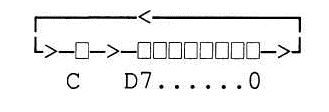
\includegraphics[width=0.45\linewidth]{pinker_RCR.png}}
            \end{tabular}
            \caption{Instrukce rotací}
          \end{figure}
          
        \subsubsection{Instrukce pro práci se zásobníkem} 
          Zásobník je adresován registrem \texttt{SP}. Ten je při zásobníkových operacích 
          automaticky inkrementován či dekrementován. Navíc je však možné s ním pracovat též jako s 
          registrem zápisníkové paměti, i když ne v plném rozsahu. Lze mezi ním, ostatními registry 
          a pamětí přesunovat data, inkrementovat a dekrementovat jeho obsah, porovnávat obsah. Na 
          začátku programu je nutné nastavit \texttt{SP} a tím definovat oblast zásobníku. Běžné 
          zásobníkové operace jsou:
          \begin{lstlisting}[gobble=10]
            PUSH r ;reg -> reg, SP se pred 
                   ;zapisem posune
            POP  r ;zasobnik -> reg, SP se 
                   ;po cteni posune
            CSP  x ;komparace SP s operandem
          \end{lstlisting}
          Některé procesory mohou ukládat do zásobníku (a vybírat z něj) i obsah paměti.
          
        \subsubsection{Instrukce pro práci s indexregistry}
          Jsou možné přesuny mezi indexregistry a jinými registry (včetně SP) i pamětí, naplnění 
          indexregistrů daty, komparace, přičtení obsahu akumulátoru, inkrementace a dekrementace.
          
        \subsubsection{Instrukce skoků}
          Efektivní adresa se přesune do \texttt{PC} a program pokračuje na nové adrese. Ve 
          skokových instrukcích se využívá přímá adresa, nepřímá adresa, indexová adresa a 
          relativní adresa. U některých jednodušších procesorů jsou tyto možnosti omezeny, 
          nejčastěji na přímou a relativní adresu. Nepřímá (zvláště indexová) adresa však dává 
          možnost velmi zajímavých programových struktur, jako je např. \emph{„rozeskakovací 
          tabulka"}. V adresové části instrukce je adresa začátku tabulky, v indexregistrech pořadí 
          v tabulce, a efektivní adresa tedy ukazuje do tabulky na místo, kde je teprve adresa 
          pokračování programu. Všechny informace o různých pokračováních programu jsou tak 
          soustředěny na jednom místě. Je-li tabulka v RAM, lze její obsah kdykoliv změnit, místo 
          aby se musely měnit adresu skoků, rozmístěné na mnoha různých místech programu.
          
          Skoky mohou být \textbf{nepodmíněné} nebo \textbf{podmíněné}. Podmínkou pak jsou 
          jednotlivé příznakové bity a jejich kombinace, nebo stav jednobitové proměnné. Adresa v 
          podmíněných skocích je zpravidla relativní. U procesorů Intel bývá instrukce pojmenována 
          jako J ... Jump = skoč), u procesorů Motorola jako BRcc\footnote{Symbolické názvy 
          podmínek „cc" podle příznakových bitů a jejich kombinací jsou vysvětleny v dalším textu.} 
          (branch = rozvětvi).
          \begin{lstlisting}[gobble=10]
            JMP x         ;nepodmineny skok na adresu "x"
            Jcc x         ;podm. skok, podm. "cc" 
                          ;z priznaku 
            Jcc bitaddr,x ;podm. skok, podm. "cc" 
                          ;podle 1bitove prom.
            Bcc x         ;alternativni jmeno k Jcc
          \end{lstlisting}
          
        \subsubsection{Instrukce smyček}
          Tyto instrukce umožňují opakované provádění programových smyček (cyklů) s předvoleným 
          počtem opakování. Jako počítadlo průchodů smyčkou figuruje některý z registrů (někdy je 
          pevně dán jen jediný), který je na začátku instrukce automaticky dekrementován 
          (některé procesory umožňují alternativně i inkrementaci) a není-li pak jeho obsah nulový, 
          provede se relativní skok. Je-li jeho obsah nulový, skok se již neprovede a přejde se na 
          další instrukci. Má-li se jednat o smyčku, má praktický význam hlavně skok zpět v 
          programu.
          \begin{lstlisting}[gobble=10]
            LOOP   reladdr   ;registr-pocitadlo pevne dan 
            DJNZ   r,reladdr ;registr-pocitadlo volitelný
          \end{lstlisting}
          
        \subsubsection{Instrukce volání podprogramů a návratu} 
          Do zásobníku se automaticky uloží adresa návratu (přesněji adresa pokračování v původním 
          programu). Efektivní adresa se přesune do \texttt{PC} a program pokračuje na nové adrese. 
          Na rozdíl od skoku, kdy se neukládá adresa návratu, je z podprogramu možný návrat ihned 
          za instrukci, která podprogram volala (viz \texttt{RET}). V adresové části instrukce může 
          být přímá, nepřímá i relativní adresa. 
          Jednodušší procesory se omezují jen na absolutní adresu.
          \begin{lstlisting}[gobble=10]
            CALL x ;voláni podprogramu
            JSR x  ;"Jump to subroutine"
                   ;neplest se skokem (JMP)!
            BSR x  ;"branch to subroutine" 
                   ;neplest se skokem (BR)!
          \end{lstlisting}
          Při návratu se automaticky ze zásobníku přesune zpět do PC adresa návratu.
          \begin{lstlisting}[gobble=10]
            RET  ;navrat z podprogramu
            RETI ;navrat z interruptového podprogramu
          \end{lstlisting}
          
          Návrat z interruptového podprogramu se liší od návratu z obyčejného podprogramu 
          (vyvolaného \texttt{CALL}). U některých procesorů se totiž při vyvolání přerušení ukládá 
          automaticky do zásobníku nejen adresa návratu, ale i další informace (např. stav registru 
          \texttt{PSW}, \texttt{CCR}, atd.). Při návratu se pak musí ze zásobníku vybrat i tyto 
          informace, takže \texttt{RETI} je zcela neslučitelná s \texttt{RET}, která vybírá jen 
          adresu návratu. Dále je nutné návrat signalizovat řadiči přerušení, který při ukončení 
          interruptového podprogramu musí posunout hladinu priority.
          
        \subsubsection{Instrukce vstupu a výstupu}
          Jako specializované instrukce existují jen u některých procesorů. Umožňují adresování 
          vstupních a výstupních (\texttt{I/O}) obvodů (případně i jiných periferních obvodů) 
          odděleně od paměti. Vyvolají patřičný vstupní či výstupní sběrnicový cyklus, ve kterém 
          jsou aktivovány \texttt{I/O} obvody.
          
          \begin{lstlisting}[gobble=10]
            IN  inaddr  ;presun ze vstupni brany do A
            OUT outaddr ;presun z A do vystupni brany
          \end{lstlisting}        
          Rozsah adres \texttt{inaddr}, \texttt{outaddr} je vždy podstatně menší než v případě 
          instrukcí přesunu z paměti. Většina procesorů ale pracuje s \texttt{I/O} obvody jako s 
          pamětí (jsou „mapovány do paměti") a pak tento typ instrukcí není vůbec realizován.
          
        \subsubsection{Instrukce pro řízení procesoru}\label{MIT:sssec_inst_cpu_cntrl} 
          Jsou velmi rozmanité, neboť úzce souvisejí s architekturou procesoru a počítače. Zde bude 
          uvedeno jen několik instrukcí, které se běžně vyskytují.
          
          \begin{lstlisting}[gobble=10]
            NOP ;prazdna operace
          \end{lstlisting}
          Procesor nevykoná žádnou činnost. Jen \texttt{PC} je inkrementován, takže program 
          postoupí na další instrukci. Ačkoliv zdánlivě je tato instrukce zbytečná, je naopak 
          využívána velmi často. Jedna nebo více \texttt{NOP} může sloužit jako časová výplň pro 
          přesné doladění časování programu, jejich skupina může vyplnit úsek v programové paměti, 
          kde se program teprve v budoucnu doplní, může nahradit některé instrukce při ladění 
          programu, atd.
          
          \begin{lstlisting}[gobble=10]
            STI ;povoleni preruseni
            CLI ;blokovani preruseni
          \end{lstlisting}
          Instrukce se vztahují k maskovatelným přerušením. Nastaví nebo nulují řídicí bit 
          přerušení, který je součástí stavového slova programu (\texttt{PSW}), a který povoluje či 
          blokuje činnost řadiče přerušení. U mnoha procesorů je však \texttt{PSW} umístěno v poli 
          řídicích a stavových registrů, se kterými se pracuje jako s datovou, bitově 
          adresovatelnou pamětí. Výše uvedené instrukce pak neexistují.
          
          \begin{lstlisting}[gobble=10]
            IDLE ;tez WAIT, snizený prikon, osc. bezi
            STOP ;tez PWRDN, SLEEP min. prikon, osc. stop
          \end{lstlisting}
          Obě instrukce zastavují procesor, který je hlavním konzumentem proudu. V prvém případě 
          však není zastaven generátor hodinových impulzů, takže zůstávají v činnosti ostatní 
          obvody počítače (to se týká zvláště jednočipových počítačů). Stav \texttt{IDLE} může být 
          ukončen přerušením (bylo-li však povoleno), jiným vnitřním signálem počítače (časovačem) 
          nebo signálem \texttt{RESET}. Ve druhém případě (\texttt{STOP}) je zastaven i generátor 
          hodinových impulzů, takže příkon je minimalizován. Ukončení je možné jen signálem 
          \texttt{RESET}.
          
        \subsubsection{Instrukce pro ladění programů}. 
          Umožní nastavení režimu krokování po instrukcích, zavedení bodů zastavení, přečtení a 
          naplnění registrů či oblasti paměti, atd. Jsou velmi závislé na architektuře procesoru.
          
        \subsubsection{Speciální instrukce} 
          Předcházející stručný výčet typických instrukcí nemohl zahrnout všechny 
          speciální instrukce, které se vyskytují třeba jen u jednoho typu procesoru od jednoho 
          výrobce. Jsou mnohdy velmi komplikované a mohou nahradit celé úseky programů pro 
          statistické výpočty, zpracování signálů, fuzzy řízení, apod.

    \subsection{Využití příznakových bitů v instrukcích podmíněných skoků}
      Příznakové bity jsou využívány hlavně v instrukcích podmíněných skoků, které umožňují větvení 
      programů. Jako podmínka pro provedení skoku mohou sloužit jednotlivé příznakové bity i jejich 
      kombinace. Lze tak vyjádřit mnoho různých podmínek. K nastavení příznakových bitů slouží 
      nejčastěji instrukce porovnání (\texttt{CMP}) nebo též aritmetické instrukce a některé 
      instrukce posunů a rotací. Zdaleka ne všechny procesory však mají úplnou sestavu níže 
      uvedených instrukcí.
      
      Nejjednodušší jsou podmínky, dané stavem jen jednoho z příznakových bitů:
      \begin{table}[ht!]
        \begin{tabular*}{0.75\textwidth}{lll}
         \textbf{Název} & \textbf{Branch if....}  & \textbf{Podmínky}   \\ \cline{1-3}
         \textbf{BCC}   & Carry Clear      & C = 0   \\
         \textbf{BCS}   & Carry Set        & C = 1   \\
         \textbf{BVC}   & Overflow Clear   & V = 0   \\
         \textbf{BVS}   & Overflow Set     & V = 1   \\
         \textbf{BMI}   & Minus            & N = 1   \\
         \textbf{BPL}   & Plus             & N = 0   \\
        \end{tabular*}
        \caption*{ }
      \end{table}
      
      V případě práce s čísly lze po předcházejícím porovnání (\texttt{CMP}) zjistit vzájemné 
      relace dvou čísel. Podmínka skoku se vztahuje k prvému operandu instrukce \texttt{CMP} 
      (případně implicitně k obsahu akumulátoru) v porovnání s druhým operandem. Jedná-li se o 
      čísla bez znaménkového bitu („unsigned integer"), jsou využívány bity \texttt{C} a \texttt{Z}:
      
      \begin{table}[ht!]
        \begin{tabular*}{0.75\textwidth}{lll}
         \textbf{Název} & \textbf{Branch if....}  & \textbf{Podmínky}   \\ \cline{1-3}
         \textbf{BEQ}   & Equal            & z = 1       \\
         \textbf{BNE}   & Not Equal        & Z = 0       \\
         \textbf{BHI}   & Higher           & C + Z = 0   \\
         \textbf{BLO}   & Lower            & C = 1       \\
         \textbf{BHS}   & Higher or Same   & C = 0       \\
         \textbf{BLS}   & Lower or Same    & C + Z = 1   \\
        \end{tabular*}
        \caption*{ }
      \end{table}
      
      Je třeba si uvědomit, že stav příznakových bitů po \texttt{CMP} je výsledkem odečtení dvou 
      čísel. Byla-li shodná (\emph{Branch if Equal}), je výsledek nulový a tudíž Z = 1. Bylo-li 
      prvé číslo větší než druhé, nemůže vzniknout přenos do bitu C a ani nemohl být výsledek 
      nulový, tudíž C + Z = 0. Podobně i v ostatních případech.
      
      V případě \textbf{čísel se znaménkovým bitem} je nejvyšší bit znaménkový a bude třeba vzít do 
      úvahy i bit přetečení \texttt{V} (symbol \(\oplus\) značí operaci EX-OR čili nonekvivalenci):
      
      \begin{table}[ht!]
        \begin{tabular*}{0.75\textwidth}{lll}
         \textbf{Název} & \textbf{Branch if....}  & \textbf{Podmínky}   \\ \cline{1-3}
         \textbf{BGT}   & Greater Than     & Z + (N \(\oplus\) V) = 0       \\
         \textbf{BLT}   & Less Than        & N \(\oplus\) V = 1       \\
         \textbf{BGE}   & Greater or Equal & N \(\oplus\) V = 0   \\
         \textbf{BLE}   & Less or Equal    & Z + (N \(\oplus\) V) = 1       \\
        \end{tabular*}
        \caption*{ }
      \end{table}

  \section{Obvody počítače}\label{MIT:chap_obv_pc}
    V této kapitole budou popsány obvody pro řízení počítače. Především se to týká řízení jednotek, 
    připojených na sběrnice. Budou zdůrazněny rozdíly mezi počítačem, složeným z několika 
    integrovaných obvodů (procesor a další) a počítačem na jediném integrovaném obvodu. V prvém 
    případě se bude jednat o počítač \textbf{vícečipový} nebo též jednodeskový, ve druhém o 
    \textbf{jednočipový} mikropočítač. U vícečipového počítače jsou všechny jednotky, nutné pro 
    jeho činnost, vnější vzhledem k procesoru. U jednočipové verze jsou již na čipu integrovány a 
    vnějším jednotkám se pokud možno vyhýbáme, tak aby byl celý systém realizován minimálním počtem 
    integrovaných obvodů. Někdy je však \emph{rozšíření} o vnější jednotky nutné, pokud rozsah nebo 
    skladba vnitřních jednotek pro danou aplikaci nestačí. Konstruktéři jednočipových mikropočítačů 
    vždy musí šetřit s počtem vývodů pouzdra (ten značně ovlivňuje cenu) a proto jsou nuceni 
    využívat některé vývody pro dvě či více funkcí. Vývody mají \emph{alternativní význam}. 
    Příkladem mohou být vývody vstupních a výstupních obvodů, které se alternativně využívají k 
    rozšíření jako vývody vnějších sběrnic. Ty pak již samozřejmě nemohou sloužit pro původní 
    funkci. Nedostatek paralelních bran bývá citelným důsledkem rozšiřování o vnější obvody.
    
    Je zřejmé, že jednočipové řešení bude mít jak společné vlastnosti s řešením vícečipovým, tak 
    vlastnosti velmi specifické. U vícečipového řešení je snadno možné na plošném spoji různě 
    \emph{propojovat} a zpracovávat vstupy a výstupy jednotlivých integrovaných obvodů a tím 
    realizovat jejich různé funkce. U jednočipového řešení jsou všechny vnitřní jednotky 
    \emph{nedostupné}. Jejich nejrůznější vzájemné vazby musí již předem existovat a programátor si 
    z nich vybere. K výběru slouží soustava \textbf{řídicích registrů}, která se může rozrůst do 
    velmi značných rozměrů (i přes stovku). Program pro takový jednočipový mikropočítač pak na 
    začátku, ještě před vlastním aplikačním programem, obsahuje \emph{inicializační část} pro 
    naprogramování řídicích registrů. Inicializace má zcela klíčovou důležitost a může výrazně 
    ovlivnit výpočetní výkon celého systému.
    
    Ke spojení procesoru s ostatními obvody počítače slouží soustava \textbf{sběrnic}. Základní 
    uspořádání a jednoduché časové diagramy byly uvedeny již v kapitole \ref{MIT:chap_BasicFceP}. 
    Vnější sběrnice jsou vyvedeny z procesoru, je-li samostatným integrovaným obvodem, nebo z 
    jednočipového mikropočítače, je-li nutné jeho vnitřní obvody rozšířit. Znalost signálů vnějších 
    sběrnic a jejich časování je nutná pro návrh systému vnějších obvodů. \emph{Posloupnost 
    činností}, během kterých dojde právě jednou ke \emph{čtení nebo zápisu} prostřednictvím 
    (vnějších) sběrnic, se nazývá (vnější) \textbf{sběrnicový cyklus} (angl. \emph{bus cycle}). 
    Základními sběrnicovými cykly jsou \textbf{cyklus čtení z paměti} a \textbf{cyklus 
    zápisu do paměti}. Vedle toho mohou existovat i další sběrnicové cykly, jako např. \emph{čtení 
    ze vstupních obvodů, zápis do výstupních obvodů}, aj. Časování signálů může být v těchto 
    cyklech odlišné.
    
    \subsection{Systémový řadič}
      Budeme se blíže věnovat hlavně signálům řídicí sběrnice. V nejjednodušším případě jsou tyto 
      signály generovány přímo procesorem, u dokonalejších architektur jsou generovány obvodem, 
      zvaným \textbf{systémový řadič} (angl. \emph{system controller}. Jiná situace nastává u 
      počítače vícečipového a jiná u jednočipového. V prvém případě může konstruktér systému využít 
      řídicí signály procesoru buď přímo, nebo přes vnější systémový řadič, jehož funkci může 
      navrhnout v souladu se zamýšlenou architekturou počítače. Pro spolupráci se systémovým 
      řadičem je procesor vybaven několika výstupními signály (např. třemi), kterými je na začátku 
      každého sběrnicového cyklu definován jeho \emph{typ} - např. \emph{čtení z paměti, zápis do 
      paměti, čtení ze vstupních obvodů}, atd. Systémový řadič pak samostatně generuje řídicí 
      signály podle typu cyklu. Pro jejich přesné časování jsou do systémového řadiče zavedeny 
      hodinové impulzy procesoru - viz obr. \ref{MIT:fig_ext_sys_radic}.
    
      \begin{figure}[ht!] %\ref{MIT:fig_ext_sys_radic}
        \centering
        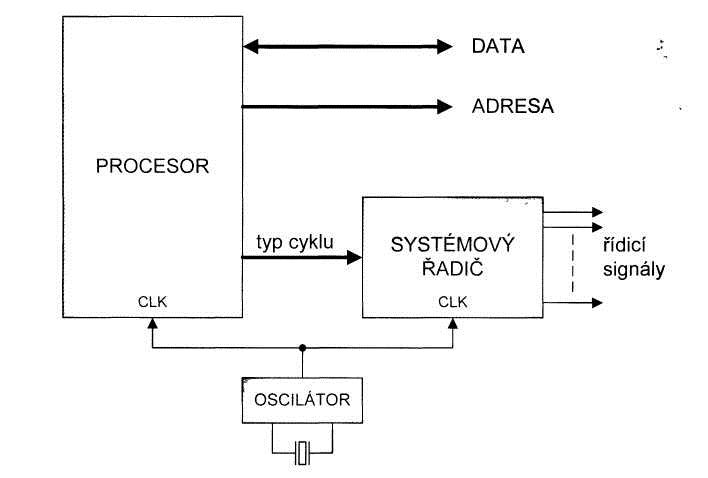
\includegraphics[width=0.9\linewidth]{pinker_ext_sys_radic.png}
        \caption{Vnější systémový řadič}
        \label{MIT:fig_ext_sys_radic}
      \end{figure}
      
      U jednočipového počítače existuje systém \textbf{vnitřních sběrnic} a též vnitřní systémový 
      řadič. Obojí je optimalizováno z hlediska rychlosti a do řízení vnitřních sběrnic nelze 
      zasahovat. Pro případné rozšíření o vnější obvody je však počítáno s vývody adresové, datové 
      a řídicí sběrnice. Aby příliš nenarůstal počet vývodů pouzdra, jsou pro vnější sběrnice 
      využity vývody již jednou obsazené - typicky jsou to vývody paralelních bran.
      
      Zvláště u 16bitových mikropočítačů umožňuje systémový řadič činnost vnějších sběrnic v 
      několika různých režimech a s různým časováním signálů. Lze přenášet slova 16bitová nebo 
      8bitová, adresovou a datovou sběrnici lze sdružit do jedné multiplexní sběrnice, lze měnit 
      časování jednotlivých signálů, atd. Režim činnosti vnějších sběrnic lze měnit prostřednictvím 
      naprogramování systémového řadiče, který je k tomu účelu vybaven řídicím registrem, nazývaným 
      \textbf{konfigurační registr}, též \texttt{MODE} registr.
       
      \begin{figure}[ht!] %\ref{MIT:fig_int_sys_radic}
        \centering
        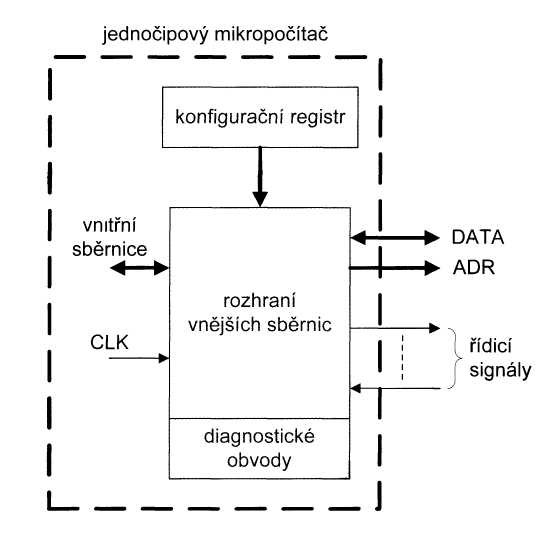
\includegraphics[width=0.7\linewidth]{pinker_int_sys_radic.png}
        \caption{Vnější systémový řadič}
        \label{MIT:fig_int_sys_radic}
      \end{figure}
    
      Konfigurační data musí být uložena do konfiguračního registru při náběhu napájení počítače 
      nebo bezprostředně po něm. V případě jednočipového mikropočítače je absolutně nutná informace 
      o rozšíření o vnější obvody, zvláště o programovou paměť - ta může být vnitřní (na čipu) nebo 
      vnější. Stejně důležité jsou i údaje o šířce vnějších sběrnic (zvláště datové) a o jejich 
      řízení a časování. Bez těchto informací se počítač nemůže rozběhnout a proto jsou příslušné 
      bity konfiguračního registru nastavovány hardwarovými prostředky během nulování počítače. 
      Druhá část bitů konfiguračního registru se týká takových signálů a činností počítače, které 
      mohou být definovány až po začátku programu, a registr tedy může být částečně naplněn až 
      samotným programem - typicky se to týká např. prostředků pro ladění programů. Zápis do 
      konfiguračního registru je vždy znesnadněn a obsah registru je chráněn před náhodným 
      přepsáním. Ochrana je řešena tak, že přístup do registruje možný jen po stanovený (a malý) 
      počet hodinových impulzů procesoru po skončení signálu \texttt{RESET}, nebo po každém 
      vynulování je zápis do něj povolen jen jednou a případné další zápisy jsou blokovány (čtení 
      blokováno není).
      
      Hardwarové prostředky pro určení konfigurace mohou u jednoduchých architektur být velmi 
      omezené a jednoduché. Jeden vývod pouzdra je vyhrazen pro konfigurační vstup, na který je 
      přivedeno napětí logické \texttt{0} nebo \texttt{1}. Bývá označen jako \texttt{EA} (angl. 
      \emph{External Access}) nebo \texttt{MP/MC} (\emph{Microprocessor/Microcomputer s 
      vnější/vnitřní pamětí}). U dokonalejších architektur by byl zapotřebí větší počet takovýchto 
      vývodů pouzdra, což je zřejmě nevhodné (s vývody pouzdra se vždy šetří). Proto jsou pro vstup 
      konfigurační informace využívány vývody jiných signálů. Po dobu aktivního signálu 
      \texttt{RESET} mikropočítač od těchto vývodů odpojí své vnitřní obvody a čte na 
      nich stav. Pomocné vnější obvody pak musí během aktivního signálu \texttt{RESET} na tyto 
      vývody vnutit stav \texttt{0} nebo \texttt{1}. Po skončení \texttt{RESET} naopak musí být 
      tyto pomocné vnější obvody odpojeny, tak aby nebyla rušena řádná činnost vývodů při běhu 
      programu. Jednoduché uspořádání ukazuje obr. \ref{MIT:fig_konfig_sys_radic}.
    
      \begin{figure}[ht!] %\ref{MIT:fig_konfig_sys_radic}
        \centering
        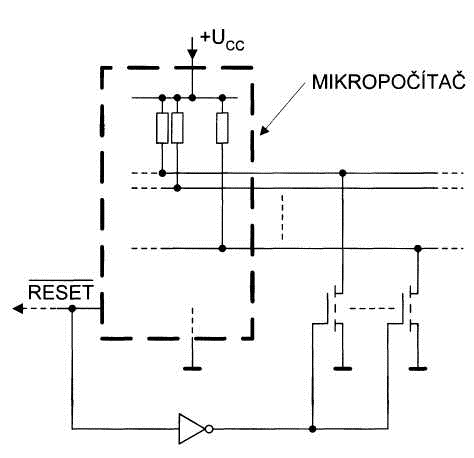
\includegraphics[width=0.7\linewidth]{pinker_konfig_sys_radic.png}
        \caption{Vnější systémový řadič}
        \label{MIT:fig_konfig_sys_radic}
      \end{figure}
    
      Stav \texttt{0} je zajištěn uzemněním patřičného vývodu tranzistorem, stav \texttt{1} odporem 
      od napájecího napětí - ten je zpravidla již realizován na čipu. Přítomnost či nepřítomnost 
      uzemňujícího tranzistoru tedy definuje stav \texttt{0} či \texttt{1} patřičného bitu 
      konfigurační informace. V praxi lze místo jednotlivých tranzistorů využít obvody s otevřenými 
      kolektory nebo obvody \texttt{GAL} s třístavovými výstupy.
      
    \subsection{Vnější sběrnice a řídicí signály}\label{MIT:chap_extbus_sign}
      Na datovou sběrnici jsou vnější jednotky vždy připojeny \emph{přes třístavové členy}, které 
      musí být řízeny tak, aby v žádném okamžiku nemohlo dojít k současnému připojení dvou nebo 
      více jednotek, což se nazývá \textbf{konflikt na sběrnici}. Přitom vždy dojde k chybě ve 
      čtených datech, ale může dojít i ke zničení třístavových členů. Bezkonfliktní výběr vždy jen 
      jedné jednotky zajišťují \emph{výběrové signály} \textoverline{\texttt{CS}}, generované 
      \textbf{adresovým dekodérem}. Jako u většiny kombinačních obvodů, i u adresového dekodéru 
      existují \emph{hazardní stavy}, které se projevují jako falešné, krátké impulzy na výstupech. 
      Proto signály z dekodérů nesmí nikdy samy spouštět činnost jednotek, nýbrž jen vybranou 
      jednotku odblokují (aktivují), zatím co vlastní výkonný povel je časován jinými řídicími 
      signály. Obecné uspořádání ukazuje obr. \ref{MIT:fig_sbernice01}.
 
      \begin{figure}[ht!] %\ref{MIT:fig_sbernice01}
        \centering
        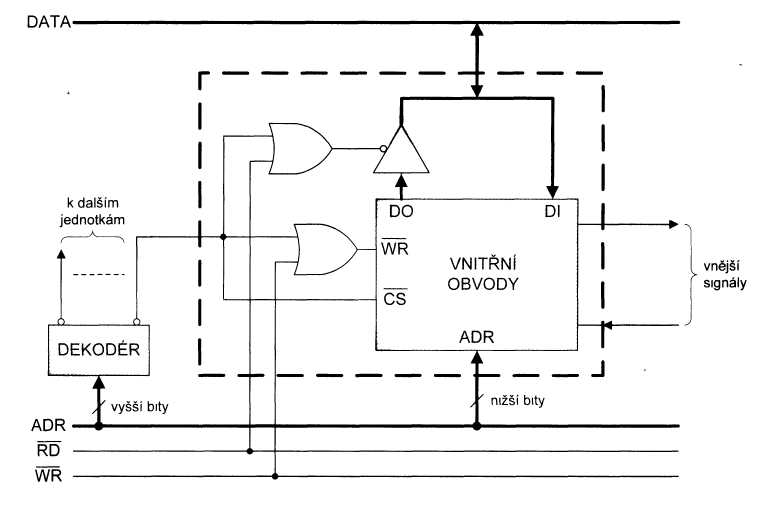
\includegraphics[width=0.7\linewidth]{pinker_sbernice01.png}
        \caption{Řízení jednotky připojené na sběrnice}
        \label{MIT:fig_sbernice01}
      \end{figure}
      
      Vlastní vnitřní obvody jednotky (v obdélníku uvnitř) jsou obecně zdrojem i příjemcem dat z 
      datové sběrnice. Jednotka je vybrána jedním výstupem adresového dekodéru. Při čtení dat je 
      tak blokován či povolen čtecí impulz, který vyvolá rychlé připojení třístavového členu. Při 
      zápisu pak je obdobně blokován či povolen průchod zápisového impulzu do vnitřních obvodů. 
      Výběrový signál\textoverline{\texttt{CS}} může, ale nemusí být zaveden do vnitřních obvodů. 
      Je-li do nich zaveden, může jednotky, které nejsou vybrány, uvádět do \textbf{úsporného 
      režimu} se sníženým příkonem (typické u pamětí). Návrat do normálního režimu u vybrané 
      jednotky vyžaduje jistou dobu - ta je zajištěna předstihem \textoverline{\texttt{CS}} před 
      čtecím či zápisovým impulzem. Jednotka může zpracovávat vnější signály. Tato činnost není 
      ovlivněna výběrovým signálem \textoverline{\texttt{CS}}.
      
      \begin{figure}[ht!]
        \centering  
        \begin{tabular}{cc}
          \subfloat[cyklus čtení]{\label{MIT:fig_sbernice02}
            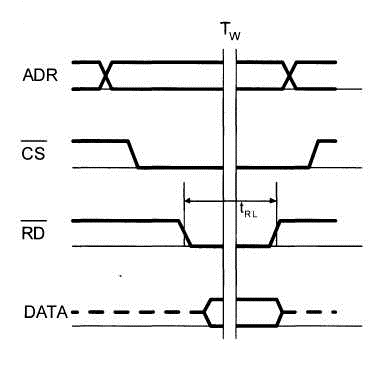
\includegraphics[width=0.45\linewidth]{pinker_sbernice02.png}}              &
          \subfloat[cyklus zápisu]{\label{MIT:fig_sbernice03}
            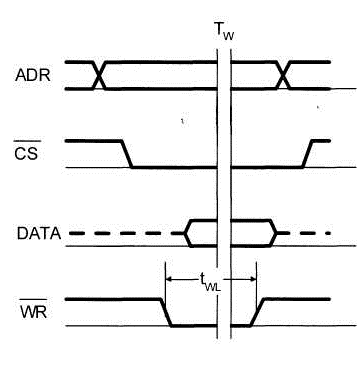
\includegraphics[width=0.45\linewidth]{pinker_sbernice03.png}}              \\
        \end{tabular}
        \caption{Základní sběrnicové cykly}
        \label{MIT:fig_sbernice0203}
      \end{figure}
    
      Nejjednodušší typ sběrnicového cyklu využívá pouze dva řídicí signály, 
      \textoverline{\texttt{RD}} a \textoverline{\texttt{WR}}. \textbf{Průběh čtení} ukazuje obr. 
      \ref{MIT:fig_sbernice02}. Počátkem je okamžik, kdy procesor vydá adresu, ze které bude číst 
      nová data. Čtecí impulz \textoverline{\texttt{RD}} je vydán, až když jsou vnitřní obvody 
      jednotky uvedeny do pohotového stavu signálem  \textoverline{\texttt{CS}} \texttt{= 0}, který 
      je generován dekodérem adres. Výstupy dekodéru se mění se zpožděním po změně adresy. K 
      výstupu dat na datovou sběrnici dochází jen s malým zpožděním po změně 
      \textoverline{\texttt{RD}}. Platná data na sběrnici pak přebírá procesor. Mimo aktivní stav 
      čtecího povelu (\textoverline{\texttt{RD}} \texttt{= 0}) je sběrnice ve vysokoimpedančním 
      stavu. Adresa zůstává konstantní až do konce čtecího povelu. Může se stát, že jednotka, ze 
      které se čte, má příliš velké zpoždění ve výstupu dat, a že data ještě nejsou ustálena v 
      době, kdy je vzorkuje procesor. Dojde tak k chybě ve čtení dat. Situaci může vyřešit vložení 
      tzv. čekacích taktů \texttt{Tw} (\texttt{WAIT}), na místě vyznačeném v obrázku dvojicí čar. 
      Prodlouží se doba platné adresy a čtecí impulz. Jednotka má k dispozici delší čas na vydání 
      platných dat. Časování signálů je odvozeno od hodinových impulzů procesoru (na obrázku nejsou 
      znázorněny). Jsou jimi časovány i čekací takty.
      
      \textbf{Průběh zápisu} ukazuje obr. \ref{MIT:fig_sbernice03}. Procesor vydá novou adresu a s 
      jistým zpožděním pak i data. Do jednotky, která byla vybrána signálem  
      \textoverline{\texttt{CS}}, jsou data zapsána impulzem \textoverline{\texttt{WR}}. I zde se 
      může stát, že jednotka je příliš pomalá a doby, znázorněné v obrázku, jsou příliš krátké. 
      Dojde tak k chybě v zápisu dat. Situaci opět může vyřešit vložení čekacích taktů \texttt{Tw} 
      na místě, vyznačeném v obrázku dvojicí čar.
     
      U různých počítačů existují různé soustavy řídicích signálů, mnohdy tradičně dodržované 
      jednotlivými výrobci a úzce související s architekturou počítače. V předchozím textu se 
      jednalo o velmi jednoduchý systém dvou řídicích signálů \textoverline{\texttt{RD}} a 
      \textoverline{\texttt{WR}}, vhodný pro architekturu s jediným adresovým prostorem. Zmíníme se 
      ještě o několika dalších soustavách. Výčet zdaleka nebude vyčerpávající.
      
      \begin{figure}[ht!]
        \centering  
        \begin{tabular}{cc}
          \subfloat[ ]{\label{MIT:fig_sbernice04}
            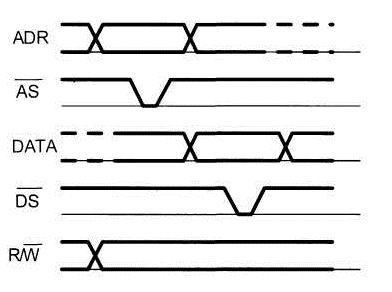
\includegraphics[width=0.45\linewidth]{pinker_sbernice04.png}}              &
          \subfloat[ ]{\label{MIT:fig_sbernice05}
            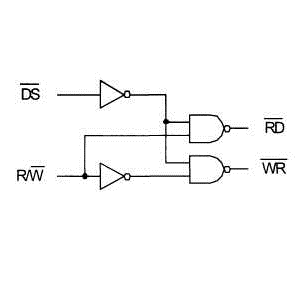
\includegraphics[width=0.45\linewidth]{pinker_sbernice05.png}}              \\
        \end{tabular}
        \caption{Sběrnicový cyklus s potvrzeními platnosti adresy}
      \end{figure}
      
      \begin{itemize}\addtolength{\itemsep}{-0.5\baselineskip}
        \item Soustava \texttt{MEMR, \textoverline{MEMW}, IOR, IOW , INTA} (\emph{Memory Read,  
              Memory Write, Input-OutputRead, Input-Output\-Write, Interrupt Acknowledge}). Signály 
              jsou časovány přibližně podle obr. \ref{MIT:fig_sbernice0203}, pro periferní obvody 
              jsou zvláš\-tní signály, \texttt{INTA} slouží pro spolupráci procesoru s řadičem 
              přerušení - viz další kapitoly.
        \item Soustava \texttt{RD, WR, PSEN} (\emph{Read, Write, Program Store Enable}). Prvé 
              dva signály řídí čtení a zápis dat, \texttt{PSEN} slouží výhradně pro čtení z vnější 
              paměti programu, je aktivní jen při čtení instrukce. Vnější adresový prostor je tak 
              rozdělen na dva prostory se stejnými adresami - programový a datový.
        \item Soustava \texttt{RD,  WR, MEM-IO}. Význam prvých dvou signálů je jako v obr. 
              \ref{MIT:fig_sbernice0203}, třetí rozlišuje mezi pamětí a periferními obvody. Mění se 
              na začátku cyklu, přibližně v době, kdy se mění adresa.
        \item Soustava \texttt{AS, DS, R/W}. Impulz \texttt{AS} (\emph{Address Strobe}) potvrzuje  
              platnost adresy, impulz \texttt{DS}  (\emph{Data Strobe}) platnost dat. Signál 
              \texttt{R/W} rozlišuje cyklus čtení (stav 1) od zápisu (stav 0) a mění se na začátku 
              cyklu. Časování ukazuje obr. \ref{MIT:fig_sbernice04} pro případ zápisového cyklu. 
              Signály této soustavy lze snadno konvertovat na signály soustavy \texttt{RD, WR} - 
              viz obr. \ref{MIT:fig_sbernice05}.
        \item Soustava \texttt{ECLK, R/W}. Sběrnicové hodiny \texttt{ECLK} nahrazují impulzy 
              \texttt{AS} (náběžná hrana \texttt{ECLK}) a \texttt{DS} (doběžná hrana 
              \texttt{ECLK}). Význam a časování \texttt{R/W} je obdobné jako v předchozím případě - 
              viz obr. \ref{MIT:fig_sbernice06}.
      \end{itemize}

      \begin{figure}[ht!] %\ref{MIT:fig_sbernice06}
        \centering
        \includegraphics[width=0.6\linewidth]{pinker_sbernice06.png}
        \caption{Sběrnicový cyklus se sběrnicovými hodinami}
        \label{MIT:fig_sbernice06}
      \end{figure}
    
      Vkládání čekacích taktů je jednoduchou metodou, jak zařídit spolupráci pomalých obvodů s 
      rychlým procesorem. Musí se samozřejmě jednat o ojedinělé cykly, aby prodlužování cyklů bylo 
      v průměru málo významné. Typicky se jedná o periferní obvody, s nimiž procesor pracuje 
      relativně zřídka ve srovnání s pamětí programu a dat. Paměti nemají sběrnicový cyklus 
      zpomalovat. Pokud ano, je nejjednodušším řešením celkové zpomalení hodinových impulzů 
      procesoru. Vkládání čekacích taktů je vyvoláno signálem na vstupu procesoru, často označeným 
      jako \texttt{READY}. Signál \texttt{READY} je v procesoru vzorkován prostřednictvím vnitřních 
      hodinových impulzů a proto je možno vkládat jen \emph{celý počet čekacích taktů} o celkové 
      délce rovné násobku periody vzorkování.
      
      Jsou dva způsoby generace tohoto signálu. V prvém případě je vytvářen v centrálním obvodu, 
      tzv. \textbf{generátor čekacích taktů} (angl. \emph{Wait-state Generator}), na základě 
      dekódování adresy. Podle příslušnosti do jedné z několika oblastí adres je vybrán příslušný 
      registr, ve kterém je předem na začátku programu zapsán údaj o délce impulzu \texttt{READY}, 
      tj. počty čekacích taktů. Registrů je několik a tak lze odstupňovat časování sběrnicových 
      cyklů pro různé periferní obvody. Druhý způsob generace \texttt{READY} spočívá v 
      decentralizaci časovacích obvodů a jejich integraci do jednotek, připojených na sběrnice. 
      Princip ukazuje obr. \ref{MIT:fig_sbernice07}.
      
      \begin{figure}[ht!] %\ref{MIT:fig_sbernice07}
        \centering
        \includegraphics[width=0.9\linewidth]{pinker_sbernice07.png}
        \caption{Decentralizované řízení sběrnicového cyklu}
        \label{MIT:fig_sbernice07}
      \end{figure}
      
      Signál \texttt{READY} vyvolá vkládání \texttt{Tw} při stavu logické nuly, což dovoluje jeho 
      generaci paralelně zapojenými obvody s otevřenými kolektory, z nichž kterýkoliv může na 
      společný vodič vnutit stav \texttt{0}. Stav \texttt{1} je zajištěn společným kolektorovým 
      odporem \(R_K\) (někdy je již vytvořen na čipu procesoru). Součástí jednotky je adresový 
      komparátor, který zjišťuje, zda adresa z adresové sběrnice spadá do oblasti adres, která 
      patří jednotce. Pokud adresa jednotce patří, je začátkem čtecího nebo zápisového 
      (\textoverline{\texttt{WR}}) impulzu spuštěn časovací obvod  (monostabilní klopný obvod 
      \texttt{MKO}) a vytvořen impulz \texttt{READY}. Zadání oblasti adres je pevně dáno, např. 
      miniaturními mechanickými spínači, nebo může být celá funkce realizována programovatelným 
      obvodem \texttt{GAL}, případně i jinými obvodovými prostředky.
      
      \subsubsection{Multiplexní sběrnice}\label{MIT:chap_mltiplex_bus} 
        Multiplexní sběrnice je využívána pro úsporu počtu vývodů pouzdra. U jednočipových 
        počítačů, kde pro vyvedení vnějších sběrnic jsou využity původní vývody bran, je úspora 
        ještě významnější. V prvé části sběrnicového cyklu je po adresové-datové sběrnici vydávána 
        adresa, ve druhé části jsou přenášena data. Adresa musí být zachycena ve vnějším adresovém 
        registru, aby byla vnějším obvodům k dispozici po celý cyklus. Zápisový impulz pro registr 
        je jedním z řídicích signálů vnější sběrnice. Ve výše popsaných soustavách řídicích signálů 
        to např. mohl být impulz \texttt{AS}, často je však označován jako \texttt{ALE} 
        (\emph{Address Latch Enable}). Zápis do registru zpomaluje sběrnicový cyklus - to 
        je daň za úsporu vývodů. Celé uspořádání a časování ukazuje obr. \ref{MIT:fig_sbernice08}.
       
        \begin{figure}[ht!] %\ref{MIT:fig_sbernice08}
          \centering
          \includegraphics[width=0.9\linewidth]{pinker_sbernice08.png}
          \caption{Multiplexní sběrnice a časování}
          \label{MIT:fig_sbernice08}
        \end{figure}
        
        Často je datová sběrnice užší než adresová (8 bitů proti 16 bitům). Pak jen 8 bitů je 
        multiplexováno jako adresa/data, zatím co zbylých 8 bitů má trvale význam adresy. V tom 
        případě jsou vždy multiplexovány nižší bity adresy - předpokládá se, že nejvyšší bity jsou 
        zavedeny do adresového dekodéru, který vytváří výběrové signály. Zpoždění dekodéru takto 
        zhruba kompenzuje zpoždění adresového registru.
        
        V případě široké datové sběrnice (16 a více bitů) mohou vnější jednotky pracovat jak s daty 
        o plné šířce, tak také s daty 8bitovými (to je dokonce mnohem častější). Osmibitové obvody 
        - zvláště paměti -  mohou být připojeny tak, že jeden je připojen na dolních 8 bitů (tj. 
        dolní slabika), druhý na horních 8 bitů dat (tj. horní slabika). Lze tak přenášet horní 
        slabiku, dolní slabiku, nebo obě současně, tj. celé slovo. Některé instrukce takovouto 
        volbu umožňují. K připojení \emph{„horní-dolní-oba"} slouží výběrové vstupy 
        \textoverline{\texttt{CS}}. Jeden způsob používá adresový bit \texttt{A0} (tj. nejnižší) a 
        přídavný signál \texttt{BHE} (\emph{byte high enable}) 
        takto:

        \begin{table}[ht!]
          \setlength{\tabcolsep}{5pt}
          \begin{tabular*}{0.75\textwidth}{lll}
            \texttt{A0}       & \textoverline{\texttt{BHE}} & Funkce  \\ \cline{1-3}
            \texttt{0} & \texttt{1} & slovo          \\
            \texttt{0} & \texttt{1} & dolní slabika  \\
            \texttt{1} & \texttt{0} & horní slabika  \\
            \texttt{1} & \texttt{1} & nepoužito      \\
          \end{tabular*}
          \caption*{ }
        \end{table}
        
        Uspořádání ukazuje obr. \ref{MIT:fig_sbernice09}. Všimněme si bitu \texttt{A0}, který je 
        zaveden jen do jednoho obvodu. Paměť je adresována po slabikách, při postupném zvyšování 
        adresy by se pravidelně střídala dolní-horní slabika podle druhé a třetí řádky tabulky. 
        Druhá možnost je na obr. \ref{MIT:fig_sbernice10} - adresový bit \texttt{A0} není vůbec 
        použit a k rozlišení slabik slouží výběrové signály \texttt{CS1} a \texttt{CS2} . Při 
        přenosu slova je vždy vhodné, aby byly obě slabiky přenášeny současně. To ale znamená, že 
        slovo musí začínat na \emph{sudé adrese} (\texttt{A0 = 0}). Pokud je adresa slova posunuta 
        o 1, musí být slovo přenášeno postupně (ve dvou cyklech). Jedná se o nesprávné 
        \textbf{zarovnání slov} (angl. \emph{misalignment}), které zpomaluje činnost počítače. 
        Překladače tuto skutečnost respektují a umožňují vhodně posunout adresy slov.
        \begin{figure}[ht!]
          \centering  
          \begin{tabular}{cc}
            \subfloat[signály \texttt{A0} a \texttt{BHE}]{\label{MIT:fig_sbernice09}
              \includegraphics[width=0.45\linewidth]{pinker_sbernice09.png}}              &
            \subfloat[výběrovými signály]{\label{MIT:fig_sbernice10}
              \includegraphics[width=0.45\linewidth]{pinker_sbernice10.png}}              \\
          \end{tabular}
          \caption{Adresování slabik a slov}
        \end{figure}
    
        Z úsporných důvodů lze dokonce systematicky pracovat jen s 8bitovými daty i u 16bitové 
        sběrnice - vyšší bity datové sběrnice nejsou vůbec využity. To sice zpomalí celý systém, 
        neboť pak bude zapotřebí dvojnásobný počet sběrnicových cyklů, ale u malých systémů se 
        zjednoduší plošný spoj a zlevní se obvody. Systémový řadič dostává informaci o šířce 
        sběrnice jako součást konfiguračních dat během nulování počítače.
    
    \subsection{Adresové dekodéry a výběrová logika}
      Každé jednotce, připojené na datovou sběrnici, je přidělená jistá oblast v adresovém 
      prostoru. Nejjednodušším řešením je adresový dekodér, který na svých výstupech generuje 
      výběrové signály pro jednotky. Podstatným nedostatkem ale je to, že dekodér dělí adresový 
      prostor na oblasti o shodné velikosti. To se zpravidla nehodí, neboť v počítači s von 
      Neumannovou architekturou zaujímá největší prostor paměť programu, pak paměť dat a velmi malý 
      prostor periferní obvody. Místo dekodéru lze navrhnout jiné kombinační obvody, což je dobré 
      řešení uvnitř jednočipového mikropočítače. Při návrhu vnějších obvodů je lépe využít 
      jednoduché programovatelné logické obvody (\texttt{GAL}) - vše je v jednom pouzdru a jsou 
      možné pozdější změny. Bez ohledu na způsob realizace budeme obvody, které vytvářejí výběrové 
      signály, nazývat \textbf{výběrovými obvody}.
      
      \begin{figure}[ht!]
        \centering  
        \begin{tabular}{cc}
          \subfloat[použití pro generaci výběrových signálů]{\label{MIT:fig_sbernice11}
            \includegraphics[width=0.45\linewidth]{pinker_sbernice11.png}}              &
          \subfloat[vnitřní zapojení]{\label{MIT:fig_sbernice12}
            \includegraphics[width=0.45\linewidth]{pinker_sbernice12.png}}              \\
        \end{tabular}
        \caption{Adresový komparátor}\label{MIT:fig_sbernice1213}
      \end{figure}
      
      Výběrové obvody mohou být s výhodou založeny na \textbf{komparátorech s maskováním}. Princip 
      ukazuje obr. \ref{MIT:fig_sbernice11}, pohled dovnitř komparátoru ukazuje obr. 
      \ref{MIT:fig_sbernice12}. Komparátor srovnává stav na jednotlivých bitech adresy se stejnými 
      bity v \textbf{registru pozice}, který udává pozici oblasti v adresovém prostoru. 
      \textbf{Registr masky} určuje, které bity adresy jsou v komparátoru ignorovány (tj. nezáleží 
      na nich). Podle schématu na obr. \ref{MIT:fig_sbernice12} je zřejmé, že bit adresy je 
      maskován při stavu \texttt{0} v registru masky. V bodu \texttt{X}, je stav \texttt{0} při 
      shodě \texttt{Ai} a \texttt{Ri} (člen \texttt{EX-OR} realizuje funkci   
      \emph{neekvivalence}), při shodě ve všech bitech je na všech \texttt{X}, stav \texttt{0} a na 
      výstupu komparátoru je pak stav \texttt{1}. Stav \texttt{0} na \texttt{M}, vnutí stav 
      \texttt{0} do bodu \texttt{X}, bez ohledu na situaci na vstupech \texttt{EX-OR}. Do 
      komparátoru jsou zavedeny jen vyšší bity adresy a bit \texttt{A0}. Počtem nejvyšších 
      nemaskovaných bitů je dán rozsah nejmenší rozlišitelné oblasti adres, maskou může být tato 
      oblast zvětšována. Nejvyšší bity, pokud nejsou maskovány, určují počátek oblasti, při které 
      komparátor dává na výstupu stav 1. Po negaci je získán výběrový signál. Manipulací s 
      jednotlivými bity v registru pozice a registru masky lze posunovat oblast adres, ve 
      kterých je výběrový signál aktivní, a též měnit velikost této oblasti.
      
      Jako příklad může sloužit komparátor, který zpracovává nejvyšších 6 bitů šestnáctibitové 
      adresy (tedy  \texttt{A15 ... A10}), registr pozice a registr masky má též šest bitů. Obsahy 
      registrů jsou např. takovéto:
      \begin{figure}[ht!] %\ref{MIT:fig_sbernice13}
        \centering
        \includegraphics[width=0.9\linewidth]{pinker_sbernice13.png}
        \caption{Příklad obsahu registru masky a pozice: Bity \texttt{A13} až \texttt{A10} jsou     
                 maskovány, proto na \texttt{R13} až \texttt{R10} nezáleží (vyznačeno jako -). 
                 Oblast adres začíná od \texttt{0100 0000 0000 0000}, tj. \texttt{4000 H}. 
                 Jelikož bity \texttt{R13} až \texttt{R10} jsou maskovány a bity \texttt{R9} až 
                 \texttt{R0} nejsou do komparátoru vedeny vůbec, je rozsah oblasti 14 bitů, tj. 
                 \texttt{16 K} adres (\texttt{1 K = 1024}).}
        \label{MIT:fig_sbernic13}
      \end{figure}
      
      Možnost programování pozice a rozsahu oblasti adres je velmi výhodná zvláště u jednočipových 
      mikropočítačů. U některých je na čipu (v rámci systémového řadiče) integrováno několik 
      adresových komparátoru a přilehlých registrů, takže z pouzdra je vyvedeno několik výběrových 
      signálů. Univerzalita může být ještě zvýšena vhodným časováním výstupů, jak ukazuje obr. 
      \ref{MIT:fig_sbernice1213}. Výstup komparátoru je logicky vynásoben se čtecím impulzem, 
      zápisovým impulzem, nebo s konstantou \texttt{1}. Výstupem je pak čtecí impulz platný jen v 
      jisté oblasti adres, zápisový impulz platný jen v jisté oblasti adres, nebo výběrový impulz 
      (\textoverline{\texttt{CS}}) - viz časování těchto impulzů v obr.      
      \ref{MIT:fig_sbernice0203}. Takto generované čtecí a zápisové impulzy mohou zrychlit činnost 
      celého počítače a ušetřit vnější obvody. Způsob časování je volen a časovací signály 
      přepínány pomocí multiplexeru na základě obsahu registru funkce.
      
      Dalším úkolem komparátoru může být rozlišení sudé a liché adresy - využití výběrových signálů 
      s touto vlastností bylo popsáno v předchozím textu. Kromě nejvyšších bitů adresy je do 
      komparátoru zaveden ještě bit nejnižší (\texttt{A0}), registr pozice a registr masky má též o 
      jeden bit víc (\texttt{R0} a \texttt{M0}). Není-li nejnižší bit zamaskován, bude záležet na 
      stavu \texttt{R0}. Je-li \texttt{R0 = 0}, bude výběrový signál aktivní při sudé adrese 
      (\texttt{A0 = 0}), je-li \texttt{R0 = 1}, bude aktivní při liché adrese.
      
      Po \emph{náběhu napájení} je však obsah registrů \emph{neznámý}, což by kromě jiného 
      znemožnilo i čtení programu. Proto jeden z výběrových signálů je \emph{pevně} určen pro 
      \textbf{paměť programu} (značen např. \textoverline{\texttt{CSBOOT}}. Registry, příslušné 
      tomuto výstupu, jsou při nulování počítače automaticky přednastaveny tak, aby se program mohl 
      rozběhnout. Registr pozice je přednastaven tak, aby oblast adres pro paměť programu 
      zahrnovala adresu, na kterou je při nulování přednastaven čítač instrukcí, velikost oblasti 
      je nastavena na maximum, atd. Na začátku programu pak jsou vhodně naprogramovány i registry 
      pro ostatní výstupy.
      
      Celý blok komparátorů a doplňkových obvodů této koncepce (angl. \emph{chip-select logic}) je 
      součástí některých jednočipových mikropočítačů s dobře propracovanou architekturou - jejich 
      činnost a programování se může částečně lišit od toho, co zde bylo popsáno, princip však je 
      obdobný. Využití adresových komparátorů je však daleko širší. Výběrové obvody mohou být 
      decentralizovány, jednotlivé komparátory mohou být součástí vnějších jednotek, připojených na 
      sběrnice. Takovéto jednotky se budou „samy" aktivovat jen v příslušných oblastech adres. 
      Místo registrů pozice a masky lze použít miniaturní spínače.
      
      Výstupy výběrových obvodů mohou mít ještě další využití. Mohou být zavedeny do 
      \emph{generátoru čekacích taktů}, který podle oblasti adres a vybavovací doby jednotky, 
      umístěné do této oblasti, vloží příslušný počet čekacích taktů do sběrnicového cyklu. Další 
      využití je v diagnostických obvodech, které kromě jiného kontrolují správnost adresy.
    
    \subsection{Paměťová mapa}
      Grafické znázornění pozice adresovatelných obvodů v adresovém prostoru se nazývá 
      \emph{„paměťová mapa"} (angl. \emph{memory map}). Název není zcela přesný, neboť zdaleka ne 
      všechny adresovatelné obvody jsou pamětí. Paměťová mapa je jednou z hlavních informací o 
      počítači a zvláště o počítači jednočipovém, který má velmi bohatý soubor periferních obvodů a 
      řídicích a stavových registrů. Příklad paměťové mapy u jednočipového mikropočítače s jedním 
      adresovým prostorem je na obr. \ref{MIT:fig_sbernice14}. Obrázek se nevztahuje k žádnému 
      konkrétnímu typu.
      
      \textbf{Oblast vektorů} na dně \textbf{oblasti programu} obsahuje v tomto příkladě adresy, 
      které procesor za zvláštních podmínek používá jako adresy skoků nebo podprogramů. Je to 
      případ \emph{„reset-vektorů"} při nulování počítače (viz další text), nebo vektorů přerušení 
      (viz příslušné kapitoly, popisující přerušení). Částí oblasti dat je vnitřní \texttt{RAM}. 
      Oblast registrů (viz detailní pohled) obsahuje jednak řídicí a stavové registry periferních 
      obvodů i procesoru a systémového řadiče (pole \texttt{SFR} - angl. \emph{Special Function 
      Registers}), jednak univerzální datové registry procesoru (pole \texttt{GPR} - angl. 
      \emph{General Purpose Registers}). U vyspělých architektur lze jak oblast vnitřní 
      \texttt{RAM}, tak oblast \texttt{GPR} přemisťovat. Přemístění \texttt{GPR} má smysl při 
      podprogramech (zvláště při přerušení) namísto úschovy obsahu pracovních registrů. Takto může 
      vzniknout téměř neomezený počet \emph{registrových bank}. Přemístění vnitřní datové paměti i 
      \texttt{GPR} má dále využití v \emph{operačních systémech reálného času}, kdy počítač 
      pracuje na několika úlohách. Každá pak může mít svoji datovou oblast a banku registrů. U 
      počítače s několika adresovými prostory existuje samozřejmě též několik paměťových map.
      
      \begin{figure}[ht!] %\ref{MIT:fig_sbernice14}
        \centering
        \includegraphics[width=0.7\linewidth]{pinker_sbernice14.png}
        \caption{Paměťová mapa}
        \label{MIT:fig_sbernice14}
      \end{figure}
      
      Po náběhu napájení jsou během nulování počítače přemístitelné oblasti nastaveny \emph{do 
      definovaných poloh} a po rozběhu programu může být jejich pozice změněna dle potřeby.
      
      Je zřejmé, že v adresovém prostoru mohou existovat prázdné oblasti, které nepatří žádným 
      obvodům. Mohou být rezervovány pro budoucí zvětšení kapacity vnitřní paměti, další periferní 
      obvody, atd.
      
    \subsection{Nulování počítače}
      Po náběhu napájení nebo po některých abnormálních stavech počítače je nutné nastavit do 
      definovaného stavu jeho řídicí registry a sekvenční logiku. K nulování procesoru slouží jeho 
      vstup \texttt{\textoverline{RESET}} (negovaný tvar je častější než nenegovaný). I některé 
      další obvody počítače jsou takovýmto vstupem vybaveny. \textbf{Zdroje nulovacího signálu} 
      jsou v podstatě tři: zásah operátora (tlačítko), kontrolní obvody napájení, vnitřní obvody 
      počítače. Negovaný tvar signálu umožňuje jednoduché zapojení obvodů, které jej generují - 
      uzemňující tlačítko, tranzistor, obvod s otevřeným kolektorem. Automatickou generaci 
      nulovacího impulzu lze snadno realizovat kondenzátorem - viz obr. \ref{MIT:fig_sbernice15}.
      
      \begin{figure}[ht!] %\ref{MIT:fig_sbernice15}
        \centering
        \includegraphics[width=0.9\linewidth]{pinker_sbernice15.png}
        \caption{Zdroje signálu pro nulování}
        \label{MIT:fig_sbernice15}
      \end{figure}
      
      Při náběhu napájení se kondenzátor nabíjí přes rezistor pomalu a po jistou dobu, dostatečnou 
      pro vynulování, se na něm udržuje napětí menší než rozhodovací úroveň vstupu. Účelem diody je 
      umožnit rychlé vybití kondenzátoru i při krátkodobém výpadku napájení. Vstupní obvod signálu 
      \texttt{\textoverline{RESET}} má vždy hysterezní charakter, aby se zabránilo případnému 
      rozkmitání obvodu při pomalých změnách na vstupu. Nulovací impulz může být generován i uvnitř 
      procesoru. Typickým zdrojem jsou diagnostické obvody. Vnitřní nulovací signál je spojen s 
      vývodem \texttt{\textoverline{RESET}}, aby byl použitelný i pro ostatní obvody počítače 
      stejně jako nulovací signál generovaný vnějšími obvody.
      
      \textbf{Kontrolní obvody napájení} jsou zdokonalenou verzí jednoduchého \texttt{RC} členu z 
      obr. \ref{MIT:fig_sbernice15}. Kontrolují překročení tolerance napájecího napětí v úzkých 
      mezích (5 až 10 \%), generují signál \texttt{\textoverline{RESET}}, přepínají napájení na 
      záložní baterii, a často mají ještě další funkce. Ukázka takového obvodu je na obr. 
      \ref{MIT:fig_sbernice16}. Obvod typicky obsahuje dva analogové komparátory. Při snížení 
      napětí zdroje na dolní toleranční mez se překlopí analogový  komparátor \texttt{AK1} a 
      přeruší přívod výběrového signálu \texttt{CS\_OUT} do paměti dat (uvede jej do stavu trvalé 
      \texttt{1}). Současně se napájení přepne na záložní baterii. Tím jsou ochráněna data v 
      paměti ještě dříve, než napájecí napětí poklesne natolik, že procesor začne fungovat 
      nespolehlivě a než může případně zničit data. Při dalším poklesu je komparátorem \texttt{AK2} 
      vynulován procesor. Nulovací signál je časovacím obvodem prodloužen ještě po náběhu napájení, 
      takže existuje v patřičné délce i při krátkodobém výpadku napájení.

      \begin{figure}[ht!] %\ref{MIT:fig_sbernice16}
        \centering
        \includegraphics[width=0.9\linewidth]{pinker_sbernice16.png}
        \caption{Kontrolní obvod napájení}
        \label{MIT:fig_sbernice16}
      \end{figure}
      
      \emph{Délka nulovacího impulzu} není libovolná, je specifikována výrobcem. Rozlišuje se 
      případ, kdy nabíhá napájecí napětí od případu, kdy nulování bylo vyvoláno vnitřními obvody 
      procesoru při nepřerušeném napětí. V prvém případě musí být nulovací impulz podstatně delší, 
      neboť oscilátor v generátoru hodinových impulzů potřebuje relativně dlouhou dobu k ustálení 
      kmitočtu - řádově desítky ms. Ve druhém případě postačí krátký impulz o délce jen několika 
      period hodinových impulzů procesoru.
      
      Nulování má vliv na řadu vnitřních obvodů procesoru i dalších částí počítače. Je zajištěn 
      takový stav řídicích registrů a dalších sekvenčních obvodů, který umožní rozběh programu. Pak 
      teprve jsou řídicí registry programem definitivně nastaveny.
      
      U všech počítačů:
      \begin{itemize}\addtolength{\itemsep}{-0.5\baselineskip}
        \item \textbf{Čítač instrukcí} je nastaven na počáteční adresu, která se u různých   
              procesorů liší. U některých procesorů je to nula, u jiných adresa blízko horního 
              kraje adresového prostoru (tak, aby tam bylo možné umístit skokovou instrukci), a u 
              některých procesorů je na stanoveném místě programové paměti uložena 
              \textbf{počáteční adresa programu} (tzv. \emph{reset-vector}) - ta je během nulování 
              přesunuta do čítače instrukcí.
        \item Jsou \emph{blokovány} obvody pro \textbf{přerušení}.
        \item \textbf{Periferní obvody} též vyžadují uvedení do definovaného počátečního stavu. To  
              se zvláště týká dvojsměrných vstupních a výstupních obvodů, u kterých je jako 
              počáteční stav vždy nastavován směr „vstup", aby nemohlo dojít ke konfliktu s 
              vnějšími zdroji signálu.
      \end{itemize}  
          
      Jen u některých počítačů:
      \begin{itemize}\addtolength{\itemsep}{-0.5\baselineskip}
        \item \textbf{Ukazatel zásobníkové paměti} (registr \texttt{SP}) je nastaven na počáteční  
              adresu zásobníku. U mnohých počítačů však není vůbec jeho počáteční obsah definován a 
              pak musí být nastaven až programem. Do té doby nelze volat podprogram nebo povolit 
              přerušení.
        \item \textbf{Generátor čekacích taktů} je nastaven na maximum pro případ pomalé    
              programové paměti. Po rozběhu programu lze počet čekacích taktů podle situace snížit.
        \item \textbf{Výběrové obvody} pro \texttt{CSBOOT} jsou nastaveny tak, že oblast 
              programové paměti souhlasí s počáteční adresou v čítači instrukcí.
        \item \textbf{Diagnostické obvody} jsou uvedeny do počátečního stavu (tj. „počítač bez  
              poruchy").
        \item Jednočipové mikropočítače obsahují velký počet řídicích registrů pro periferní     
              obvody. Jejich stav po nulování je vždy popsán ve firemní literatuře.
      \end{itemize}
      
      \textbf{Datové registry} procesoru ani \textbf{datová paměť} není nulováním nijak ovlivněna 
      (nula jako číslo totiž nemá žádnou prioritu) a jejich počáteční stav musí být zajištěn až 
      samotným programem.

    \subsection{Generace a vnitřní rozvod hodin}\label{MIT:chap_clkgen}
      Generátor hodinových impulzů je nejčastěji řízen krystalovým rezonátorem. Obvody oscilátoru 
      jsou součástí procesoru nebo jednočipového mikropočítače, rezonátor je vnější. Používá se 
      \textbf{Pierceovo zapojení} oscilátoru, vyžadující dva vnější kondenzátory - viz obr. 
      \ref{MIT:fig_sbernice17}. Jejich kapacita je doporučena ve firemní literatuře, je třeba však 
      použít též doporučený rezonátor. Při jiných rezonátorech je někdy nutné pozměnit i hodnoty 
      kondenzátorů, tak aby po zapnutí napájecího zdroje oscilátor nabíhal naprosto spolehlivě.
      
      \begin{figure}[ht!] %\ref{MIT:fig_sbernice17}
        \centering
        \includegraphics[width=0.9\linewidth]{pinker_sbernice17.png}
        \caption{Generace a rozvod hodinových impulzů}
        \label{MIT:fig_sbernice17}
      \end{figure}
      
      Moderní řešení zdroje hodinových impulzů využívá \textbf{fázový závěs} \texttt{PLL} (angl. 
      \emph{Phase Locked Loop}) ve funkci násobiče kmitočtu. Násobící činitel je dán obsahem 
      řídicího registru, při nulování počítače je kmitočet nastaven na minimum. Vzhledem k násobení 
      postačí rezonátor s nižším kmitočtem. Často se používají levné a malé „hodinkové" rezonátory 
      s rezonančním kmitočtem \SI{32.768}{\kilo\hertz}. Oscilátor s nízkým kmitočtem má menší 
      rušivé vyzařování a menší příkon.
      
      Hodinové impulzy vstupují do procesoru, kde určují základní \textbf{takty}. Strojový cyklus 
      se skládá z několika taktů - jejich počet závisí na architektuře procesoru. Prostřednictvím 
      dvou bitů v řídicích registrech procesoru lze zablokovat hodinové impulzy v procesoru nebo 
      zablokovat přímo oscilátor (viz instrukce \texttt{IDLE} a \texttt{STOP} v kapitole 
      \ref{MIT:sssec_inst_cpu_cntrl}). 
      
      U jednočipových mikropočítačů jsou dále hodinové impulzy vedeny k periferním obvodům na čipu. 
      Periferní obvody většinou potřebují hodinové impulzy o nižším kmitočtu a proto mají své 
      předděliče s programovatelným dělicím poměrem. U mnoha jednočipových mikropočítačů lze vstup 
      hodinových impulzů do periferního obvodu blokovat jedním bitem v řídicím registru obvodu a 
      tím obvod vyřadit z činnosti, není-li pro danou aplikaci potřebný.
      
      \textbf{Vyřazování obvodů} z činnosti tím, že se zablokují hodinové impulzy, je prostředkem k 
      minimalizaci \emph{příkonu}. Všechny procesory i jednočipové mikropočítače jsou vyráběny 
      technologií \texttt{CMOS}, jejíž vlastností je zanedbatelný příkon ve statickém stavu a 
      přibližně lineárně rostoucí  příkon s kmitočtem hodinových impulzů. Zablokování hodinových 
      impulzů tedy slouží stejně dobře jako odpojení napájení, ale obvod zůstane v definovaném 
      vnitřním stavu a po opětovném dodání hodinových impulzů pokračuje v původní činnosti. Po 
      odpojení napájecího napětí a jeho opětovném přivedení však obvod bude v nedefinovaném stavu a 
      je nutné jeho vynulování. Dalším prostředkem ke snížení příkonu je snížení kmitočtu 
      hodinových impulzů pro procesor. Ten je totiž největším spotřebičem a opět jeho příkon 
      je zhruba úměrný kmitočtu. Manipulace s kmitočtem generátoru je možná díky existenci fázového 
      závěsu. Kmitočet lze nastavit jen tak vysoký, jak je třeba pro danou aplikaci (ne vždy je 
      nutný maximální výpočetní výkon, úspora energie může být důležitější).
      
    \subsection{Diagnostické prostředky počítače}
      Diagnostika počítače představuje velmi rozsáhlou problematiku a týká se jak programů, tak i 
      obvodů. Ani jeden z těchto prostředků není sám o sobě dokonalý a je nutné je vhodně 
      kombinovat. Softwarové diagnostické prostředky jsou velmi pružné, mají však jednu podstatnou 
      nevýhodu - při zhroucení programu nefungují. Podstatná důležitost hardwarových prostředků je 
      proto zřejmá.
      
      Zmíníme se o nejčastějších kontrolních obvodech. Ty lze u vícečipového počítače doplnit jako 
      vnější obvody k procesoru. U jednočipového mikropočítače je kontrola vnitřních obvodů 
      záležitostí konstruktéra integrovaného obvodu. U moderních architektur je na ně pamatováno.
      
      \begin{figure}[ht!]
        \centering  
        \begin{tabular}{cc}
          \subfloat[asynchronní verze]{\label{MIT:fig_sbernice18}
            \includegraphics[width=0.45\linewidth]{pinker_sbernice18.png}}              &
          \subfloat[synchronní verze]{\label{MIT:fig_sbernice19}
            \includegraphics[width=0.45\linewidth]{pinker_sbernice19.png}}              \\
        \end{tabular}
        \caption{Diagnostický časovač}
        \label{MIT:fig_sbernice1819}
      \end{figure}
      
      Velmi častým kontrolním obvodem je \textbf{diagnostický časovač} \texttt{WDT} (angl 
      \emph{Watch-Dog Timer}). Jedná se o znovuspustitelný (angl. \emph{retriggerable}) 
      monostabilní klopný obvod nebo jeho funkční ekvivalent, který je programově spouštěn. Do 
      programu jsou vloženy instrukce pro jeho spuštění  tak často, aby se stále udržoval v 
      dočasném stavu. Při poruše ve vykonávání programu lze s velkou pravděpodobností očekávat, že 
      dojde k výpadku ve spouštění \texttt{WDT} a obvod se překlopí zpět do stabilního stavu. Tím 
      je generováno hlášení o poruše. Existují zásadně dvě verze tohoto obvodu: \emph{asynchronní 
      a synchronní} - viz obr. \ref{MIT:fig_sbernice1819}. \textbf{Asynchronní verze} na obr. 
      \ref{MIT:fig_sbernice18} je založena na analogovém principu, kdy kondenzátor je nabíjen ze 
      zdroje proudu a při dosažení jistého napětí (tj. po jistém čase) se překlopí komparátor. 
      Spínacím tranzistorem je kondenzátor čas od času vybit a tudíž napětí na něm při dostatečné 
      častém vybíjení nikdy komparátor nepřeklopí. Při nulování počítače se vybije kondenzátor a 
      výstup se uvede do neaktivního stavu, takže při náběhu programu je dostatek času na první 
      obsluhu \texttt{WDT}. Obvod vyžaduje kondenzátor o velké kapacitě, kterou nelze realizovat v 
      integrované technologii. Tento \texttt{WDT} je tedy vždy koncipován jako vnější obvod.
      
      \textbf{Synchronní verze} \texttt{WDT} - viz obr. \ref{MIT:fig_sbernice19} - využívá 
      oscilátor a za ním následující čítač se vstupem nulování. Pokud čítač počítá nahoru a je 
      dostatečně často programově nulován, nedopočítá nikdy do své plné kapacity. Pokud dojde k 
      chybě v provádění programu a ten neobsluhuje \texttt{WDT} dostatečně často, dojde k přenosu z 
      nejvyššího bitu čítače a je tak signalizována porucha. Jako u asynchronní verze, i zde je 
      během nulování počítače \texttt{WDT} blokován a jeho čítač je vynulován. Tento typ 
      \texttt{WDT} může být součástí jak vnějších obvodů (např. kontrolních obvodů napájení), tak 
      může být i uvnitř procesoru či jednočipového mikropočítače. Pokud je uvnitř, nemá svůj 
      oscilátor a využívá hodinové impulzy procesoru. V tomto uspořádání však nelze rozpoznat 
      selhání zdroje hodinových impulzů - čítač totiž přestane čítat a pak nikdy nedojde k přenosu. 
      Proto při umístění \texttt{WDT} uvnitř jsou diagnostické obvody doplněny ještě o kontrolní 
      obvod oscilátoru. Jeho výstup je logicky sečten s výstupem \texttt{WDT}.
      
      Výstupem \texttt{WDT} je zpravidla generován nulovací impulz počítače a tím může být celý 
      program nastartován znova od začátku. Toto řešení není ideální, neboť při trvalé poruše v 
      paměti programu dojde k zásahu \texttt{WDT} znova (periodicky), což musí být u zařízení s 
      vyššími nároky na spolehlivost vyloučeno. U vyspělejších architektur jednočipových 
      mikropočítačů je proto aktivita každého zdroje nulovacího signálu \textbf{identifikována}, a 
      to zápisem do příslušného bitu v jednom ze stavových registrů procesoru, nebo je patřičně 
      modifikována počáteční adresa programu - typicky existuje několik \textbf{reset-vektorů}. Při 
      náběhu se pak program větví a v případě nulování od \texttt{WDT} lze provést jinou 
      akci, než při normálním náběhu. Pokud je \texttt{WDT} ve vnějších obvodech, nemusí jeho 
      výstup způsobit nulování, nýbrž může být zaveden do speciálních \emph{havarijních obvodů}.
      
      Ke spouštění \texttt{WDT} ve vnějších obvodech lze využít jeden bit jedné výstupní brány, 
      nebo může být adresován prostřednictvím adresového dekodéru na vnějších sběrnicích. Pokud je 
      uvnitř jednočipového mikropočítače, zachází se s ním jako s registrem, který má svoji adresu 
      v prostoru periferních obvodů -jen zápis do něj je záměrně zkomplikován, aby se snížila 
      pravděpodobnost jeho falešného spouštění při „bloudění" programu v poruše. Zpravidla je do 
      registru \texttt{WDT} nutné zapsat předepsané číslo, nebo se musí zápis bezprostředně po sobě 
      dvakrát opakovat, apod.
      
      V programu je nutné \textbf{rozmístit instrukce s obsluhou} \texttt{WDT} tak, aby nebyl 
      překročen jeho nastavený čas (typicky desítky ms). Musí být proto vloženy jak v hlavní větvi 
      programu, tak v podprogramech. Je nutné zvážit dobu provádění programových smyček (zvláště 
      při iteracích) a eventuálně vložit obsluhu \texttt{WDT} i do nich. Při ladění programů je 
      nutné \texttt{WDT} blokovat - to je u jednočipových mikropočítačů možné jedním bitem registru 
      \texttt{WDT}.
      
      Diagnostická účinnost \texttt{WDT} není absolutní. Mezi výskytem poruchy a vyvoláním zásahu 
      \texttt{WDT} může uplynout dosti dlouhá doba, za kterou může vadně fungující počítač způsobit 
      řadu chybných akcí. Proto jsou využívány ještě další kontrolní obvody.
      
      \textbf{Kontrola správnosti adresy} zjišťuje, zda omylem nebyla vydána adresa, která nepatří 
      žádné z existujících jednotek počítače. Na datovou sběrnici se pak v okamžiku čtecího impulzu 
      nepřipojí žádný obvod a data, která jsou čtena, závisí na impedančním zakončení sběrnice. V 
      každém případě jsou to data nesprávná, ale program o tom nemá žádnou informaci. Pokud se 
      jedná o zápis, budou data ztracena, neboť se nikam nezapsala. Kontrolní obvody jsou založeny 
      na zpracování výběrových signálů z adresového dekodéru (případně dokonalejších výběrových 
      obvodů). Jestliže při čtecím nebo zápisovém sběrnicovém cyklu není žádný výběrový signál 
      aktivní, zřejmě byla vydána adresa neexistující jednotky a je generováno hlášení o poruše - 
      viz obr. \ref{MIT:fig_sbernice20}.
      
      Kontrola správnosti adresy nepostihuje případ, že adresovaná jednotka sice existuje, ale 
      nepracuje v důsledku své vnitřní poruchy. Důležité jednotky proto mohou být vybaveny svými 
      vnitřními diagnostickými obvody, které na konci sběrnicového cyklu potvrzují správné 
      provedení operace. Potvrzovací signály z jednotek jsou přes obvody s otevřenými kolektory 
      přivedeny na společnou potvrzovací sběrnici, zavedenou do centrálních kontrolních obvodů. Ty 
      pak kromě kontroly správnosti adresu ještě kontrolují včasné 
      potvrzení operace.
      
      \begin{figure}[ht!] %\ref{MIT:fig_sbernice20}
        \centering
        \includegraphics[width=0.9\linewidth]{pinker_sbernice20.png}
        \caption{Kontrola správnosti adresy}
        \label{MIT:fig_sbernice20}
      \end{figure}
      
      Jiným případem je \textbf{kontrola správnosti čtené instrukce}, přesněji operačního kódu. 
      Neexistující kód hlásí dekodér instrukcí, který je vnitřní částí procesoru. Mezi chybou při 
      čtení dat a při čtení instrukce je podstatný rozdíl: zatím co u dat nelze na poruchu usuzovat 
      z jejich hodnoty (všechna čísla jsou možná), u instrukce existuje jen omezený počet 
      operačních kódů (co je mimo tuto množinu, je chybou). Tyto kontrolní obvody musí být 
      zabudovány přímo v dekodéru instrukcí a nelze je realizovat dodatečně jako vnější jednotku.
      
  \section{Přerušení programu}\label{MIT:chap_irq}\hypertarget{MIT:sec_002}
    Přerušení je \emph{metoda, kterou počítač reaguje na asynchronní, neočekávanou událost a vyvolá 
    její obsluhu}. Události mohou být omezeny na vnitřní obvody procesoru nebo jednočipového 
    mikropočítače, nebo mohou být vnější vzhledem k počítači. Takovou událostí, která nastává v 
    periferních obvodech, může např. být doběhnutí časovače, změna na vstupech paralelní brány, 
    příjem znaku v sériovém přijímači, dokončený převod v A/Č převodníku a mnoho jiných. Události, 
    které mají svůj původ uvnitř procesoru, jsou typicky vyvolávány diagnostickými obvody a jsou 
    zvláštním případem událostí. Někteří výrobci je označují jako „\textbf{traps}" (pasti) na 
    rozdíl od ostatních událostí v periferních či vnějších obvodech, které jsou pak označovány jako 
    „\textbf{interrupts}" (přerušení). U jiných výrobců je používáno označení     
    „\textbf{exceptions}" (výjimky) pro obě tyto kategorie událostí.

    
    Událost vyvolá přerušení dosud běžícího programu a odskok na \textbf{obslužný podprogram}. Po 
    jeho dokončení se počítač opět vrací do přerušeného programu. V případě periferních obvodů je 
    obsluha přerušení poměrně jednoduchá a spočívá v přečtení příslušného datového registru a 
    přesunu dat do datové paměti nebo opačně, v přesunu dat z paměti do datového registru 
    periferního obvodu. Často je přitom nutné ošetřit i řídicí registry periferních obvodů tak, aby 
    byla umožněna jejich další činnost. Událost může být také podnětem pro výstupní operaci, např. 
    změnu stavu na výstupech paralelní brány.
      
    Při práci v reálném čase je třeba, aby vstupní i výstupní operace probíhaly v přísně 
    stanovených časech s malými tolerancemi. Zde je důležitým parametrem \textbf{latence přerušení} 
    (angl. \emph{interrupt latency}), což je \emph{doba od výskytu události až do začátku její 
    obsluhy}.
    
    Výskyt události je signalizován \textbf{požadavkem na přerušení} \texttt{IRQ} (angl. 
    \emph{Interrupt Request}), a to buď hladinou nebo hranou. Hladinový požadavek je aktivní po 
    celou dobu trvání stanoveného stavu - často je to logická \texttt{0} - pak tedy je značen jako 
    \texttt{IRQ} . Hranový požadavek existuje jen krátkodobě a musí být zachycen v obvodu scitlivém 
    na změnu vstupního stavu, typicky v klopném obvodu.
    
    \subsection{Řadič přerušení}
      Požadavků na přerušení je prakticky vždy větší počet. K jejich zpracování pak slouží řadič 
      přerušení (angl. \emph{interrupt controller}). Řadič úzce spolupracuje s procesorem, ale není 
      jeho součástí. U vícečipové koncepce je vnějším obvodem, nebo je integrován s dalšími 
      vnějšími obvody.
      
      Úloha řadiče je následující:
      \begin{itemize}\addtolength{\itemsep}{-0.5\baselineskip}
        \item registrovat aktivní požadavky na přerušení,
        \item v případě více než jednoho aktivního požadavku je zařadit dle priority,
        \item dodat procesoru informaci o tom, který požadavek byl vybrán, tj. identifikovat 
              zdroj požadavku,
        \item informovat procesor o tom, že existuje alespoň jeden aktivní požadavek.
      \end{itemize}
    
      Obr. \ref{MIT:fig_sbernice21} ukazuje hlavní části řadiče přerušení, řešeného jako vnější 
      obvod k procesoru.

      \begin{figure}[ht!] %\ref{MIT:fig_sbernice21}
        \centering
        \includegraphics[width=0.9\linewidth]{pinker_sbernice21.png}
        \caption{Hlavní části vnějšího řadiče přerušení}
        \label{MIT:fig_sbernice21}
      \end{figure}
      
      \textbf{Registr požadavků na přerušení} \texttt{IRR} (angl. \emph{Interrupt Request 
      Register}) uchovává vstupní požadavky \texttt{IRQ} po dobu nutnou k jejich zpracování 
      navazujícími obvody. Klopné obvody \texttt{IRR} lze naprogramovat tak, že reagují buď na 
      hladinu, nebo na hranu. U některých řadičů lze volit náběžnou nebo doběžnou hranu, někdy i 
      obě - požadavek na obsluhu je pak vyvolán každou změnou 
      stavu \texttt{IRQ}.
      
      Jednotlivé výstupy \texttt{IRR} mohou být blokovány jednotlivými bity \textbf{registru masky} 
      \texttt{IMR} (angl. \emph{Interrupt Mask Register}), takže jen ty požadavky, které jsou 
      povoleny, postupují dále. Maskování požadavků může být průběžně měněno během provádění 
      programu. \textbf{Prioritní kodér} vybírá aktivní požadavek s nejvyšší prioritou a přiřazuje 
      mu binární číslo - \texttt{IRQ0} přiřadí \texttt{000}, \texttt{IRQ1} přiřadí \texttt{001} 
      atd. Současně je vytvářen signál \texttt{INT}, kterým je informován procesor o existenci 
      požadavku na přerušení. Procesor pak zahájí komunikaci s řadičem přerušení jako první akci 
      pro zpracování přerušení. Požadavek \texttt{INT} může být maskován \textbf{bitem globální 
      masky} přerušení \texttt{IE} (angl. \emph{Interrupt Enable} - povolení přerušení) - viz obr. 
      \ref{MIT:fig_sbernice21}. U samostatných procesorů je tento bit zpravidla součástí 
      \textbf{stavového registru} \texttt{PSW} a ovládá se zvláštními instrukcemi „\emph{povol 
      přerušení}" a „\emph{zakaž přerušení}". Polarita je u různých procesorů různá - u některých 
      se přerušení povoluje stavem \texttt{1}, u jiných stavem \texttt{0}. Při nulování procesoru 
      (Reset) se přerušení vždy automaticky zakazuje.
      
      Obsah \textbf{registru obsluhovaných požadavků} \texttt{ISR} (angl. \emph{In-Service 
      Register}) udává typ přerušení. Je čteno ve zvláštním sběrnicovém cyklu „\emph{čtení typu 
      přerušení}". Na obr. \ref{MIT:fig_sbernice21} je tento cyklus doprovázen čtecím impulzem na 
      zvláštním vodiči řídicí sběrnice \texttt{INTA} (angl. \emph{Interrupt Acknowledge}), u jiných 
      procesorů mohou být k tomuto účelu využity jiné řídicí signály nebo jejich kombinace - v 
      každém případě se jedná o speciální čtecí cyklus, nezaměnitelný s jinými čtecími cykly (z 
      paměti apod.)
      
      Do řídicích registrů řadiče a do registru masky zapisuje procesor obdobně jako do ostatních 
      periferních obvodů, které mají vyhrazenu část adresového prostoru. Obsahem řídicích registrů 
      je určen režim činnosti řadiče (způsob vyhodnocení priority, způsob zachycení požadavků 
      \texttt{IRQ}, apod.). Vzhledem k existenci několika registrů je do řadiče zavedena i adresa o 
      rozsahu jednoho nebo více nejnižších bitů.

      Téměř každý procesor je vybaven ještě vstupem pro \textbf{nemaskovatelné přerušení} 
      \texttt{NMI} (angl. \emph{Non-Maskable Interrupt}), který má absolutní prioritu a není veden 
      přes řadič. Má kratší latenci než maskovatelné přerušení a nevyžaduje spolupráci procesoru s 
      řadičem. Je využíván pro havarijní případy (zablokování programu, selhání obvodů, atd.).

      \begin{figure}[ht!] %\ref{MIT:fig_sbernice22}
        \centering
        \includegraphics[width=0.7\linewidth]{pinker_sbernice22.png}
        \caption{Prioritní obvod s pevně přiřazenou prioritou}
        \label{MIT:fig_sbernice22}
      \end{figure}

      Způsobů vyhodnocení priority je několik. Nejčastější (a nejjednodušší) je \textbf{priorita} 
      podle připojení nebo též pevná priorita. Zpravidla vstup \texttt{IRQ0} má nejvyšší prioritu, 
      \texttt{IRQ1}, druhou nejvyšší, atd. Obvody takovéhoto prioritního kodéru s maskováním 
      ukazuje obr \ref{MIT:fig_sbernice22}.
      
      Požadavky zachycené v registru \texttt{IRR} jsou logicky vynásobeny s výstupy maskovacího 
      registru \texttt{IMR}. Je-li stav příslušného bitu \texttt{IMR} nula, požadavek se neuplatní. 
      Prioritní obvod  propustí požadavek \texttt{MIRQ0} vždy, \texttt{MIRQ1}, jen je-li 
      \texttt{MIRQ0} neaktivní (tj. \texttt{0}), \texttt{MIRQ2} jen jsou-li \texttt{MIRQ0} i 
      \texttt{MIRQ1} neaktivní, atd. Při libovolné kombinaci aktivních signálů \texttt{MIRQ} (stav 
      \texttt{1}) je aktivní jen jediný signál \texttt{PIRQ}. K dalšímu zpracování se proto může 
      použít běžný kodér, převádějící \textbf{kód 1 z N} na kód binární. Pokud je alespoň jeden ze 
      signálů \texttt{MIRQ} aktivní, je v součtovém členu vytvořen signál \texttt{INT}, kterým je 
      informován procesor.
      
      Dalším způsobem vyhodnocení priority (i když výjimečným) je \textbf{cyklická priorita}. Při 
      ní se s každým vykonaným obslužným podprogramem přesunuje maximální priorita o 1 místo 
      doprava, takže bude na pozici \texttt{IRQ1} druhá nejvyšší na \texttt{IRQ2} atd., až na 
      \texttt{IRQ0} bude nejnižší. Při dalším přerušení se opět posune, atd. Cyklická priorita je 
      využívána výjimečně -je vhodná tam, kdy obsluhované požadavky mají stejnou důležitost a 
      vyskytují se stejně často. Při pevně přiřazené prioritě by totiž požadavek na IRQ0 získával 
      obsluhu přednostně a na ostatní - ačkoliv stejně důležité - by nedošla řada.
      
      Dokonalejší řadiče umožňují každému požadavku přiřadit \textbf{libovolnou prioritu} s jediným 
      omezením: žádné 2 požadavky nesmějí mít priority shodné. K nastavení priorit je každý vstup 
      opatřen individuálním registrem priority. Priority lze během činnosti programu měnit. 
      Obvodové řešení vyžaduje vřazení přepínače (např. jako matice spínačů \texttt{MOS} ve funkci 
      multiplexeru) mezi maskované signály a vstupy prioritního kodéru.
      
      Mezi libovolným přiřazením priority a pevnou prioritou leží \textbf{metoda zařazení priorit 
      do úrovní}, typicky dvou. Řadič je v tom případě vybaven registrem úrovně priority, kde každý 
      požadavek \texttt{IRQ} má svůj bit, určující zařazení požadavku do úrovně priority \texttt{H} 
      (vyšší) nebo \texttt{L} (nižší). V rámci téže úrovně stále platí pevná priorita podle 
      připojení, ale požadavky ve vyšší úrovni mají vždy přednost. Tak např. při zařazení do úrovně 
      dle obr. \ref{MIT:fig_sbernice23} má požadavek \texttt{IRQ7} vyšší prioritu než 
      \texttt{IRQ0}, ale v rámci vyšší úrovně má až nejnižší prioritu. Nejvyšší prioritu ze všech 
      bude mít požadavek \texttt{IRQ3} a nejnižší \texttt{IRQ5}.
      
      \begin{figure}[ht!] %\ref{MIT:fig_sbernice23}
        \centering
        \includegraphics[width=0.8\linewidth]{pinker_sbernice23.png}
        \caption{Prioritní obvod s pevně přiřazenou prioritou}
        \label{MIT:fig_sbernice23}
      \end{figure}
      
    \subsection{Činnost procesoru a řadiče při přerušení}
      Při výskytu aktivního požadavku, který není maskován příslušným bitem v registru 
      \texttt{IMR}, je signálem \texttt{INT = 1} upozorněn procesor. Byl-li bit globální masky 
      nastaven do stavu „povoleno", je zahájena obsluha přerušení. Nejprve je dokončena momentálně 
      prováděná instrukce. Výjimkou jsou některé instrukce, jejichž dokončení by trvalo příliš 
      dlouho. Typicky jsou to u některých procesorů cyklicky probíhající instrukce pro zpracování 
      bloků dat - takovéto instrukce lze přerušit a po návratu dokončit. Pak je do zásobníku 
      uložena návratová adresa. U některých procesorů je dále uloženo stavové slovo \texttt{PSW} a 
      někdy i další důležité registry (akumulátor, indexregistry ...) - to je ale spíše 
      výjimečné. U většiny procesorů se o uložení těchto registrů musí postarat programátor.
      
      Dále procesor vyvolá cyklus čtení typu přerušení z řadiče přerušení. Přitom je v řadiči 
      nejprve zapsán typ přerušení do registru \texttt{ISR}, a pak je vynulován ten klopný obvod 
      \texttt{IRR}, kterým bylo vyvoláno přerušení. To je však typické jen u klopných obvodů 
      naprogramovaných na reakci na hranu \texttt{IRQ}. Klopné obvody řízené hladinou \texttt{IRQ} 
      se nevynulují, pokud požadavek \texttt{IRQ} trvá. Číslo, vyjadřující typ přerušení, zůstává 
      zafixováno v \texttt{ISR}. Procesor přečte typ přerušení a přiřadí mu počáteční adresu 
      obslužného podprogramu.
      
      Přiřazení může být u některých procesorů pevné, kdy každému typu přerušení je pevně přiřazena 
      jiná počáteční adresa obslužného podprogramu v programové paměti. Procesor volá podprogram na 
      této adrese. Začátky podprogramů jsou pro úsporu místa poměrně blízko sebe (několik slabik) a 
      do mezery mezi nimi se v podstatě vejde jen instrukce skoku na další pokračování podprogramu. 
      Častějším případem je interpretace typu přerušení jako \textbf{ukazatele do tabulky vektorů}. 
      Tabulka je uložena v programové paměti a jsou v ní těsně za sebou seřazeny počáteční adresy 
      podprogramů. Typ přerušení je vynásoben konstantou tak, aby jako ukazatel vždy ukazoval na 
      některou počáteční adresu. Tak např u počítače s pamětí adresovanou po slabikách a s 
      16bitovou adresou (tj. 2 slabiky) je typ přerušení vynásoben dvěma. Kdyby byla adresa 
      4slabičná, byl by vynásoben čtyřmi. Při vyvolání obslužného podprogramu procesor dosadí 
      adresu z tabulky vektorů. Je-li tabulka umístěna v paměti \texttt{RAM}, jak je tomu např. u 
      personálních počítačů, mohou být adresy obslužných podprogramů dynamicky měněny, tj. během 
      běhu programu. U počítačů určených pro řízení (\emph{vestavěné počítače}) je program i 
      tabulka typicky v paměti \texttt{ROM} a nelze je měnit. Některé procesory proto mají zvláštní 
      registr pro určení počátku tabulky, jehož obsah je sečten s ukazatelem. V paměti \texttt{ROM} 
      tak může existovat několik předem připravených tabulek a podle potřeby je vybrána jedna z 
      nich.
      
      Současně s vyvoláním podprogramu procesor nastaví globální masku přerušení na stav 
      „\emph{zakázáno}" a tím je znemožněno vyvolání dalšího přerušení během již běžícího 
      obslužného podprogramu. Pokud je existence do sebe \textbf{vložených} (angl. \emph{Nested}) 
      obslužných podprogramů skutečně nutná, může být globální maska programově nastavena na 
      „\emph{povoleno}". Dříve však, hned na začátku podprogramu, je nutné uložit do zásobníku 
      registr \texttt{PSW} a další datové registry - ne nutně všechny, ale alespoň ty, jejichž 
      obsah bude v podprogramu ovlivněn. Jak již bylo zmíněno, některé procesory tuto činnost 
      vykonávají při přerušení automaticky. Automatický zákaz přerušení na začátku podprogramu 
      zabraňuje opakovaným přerušením v případě, že přerušení bylo vyvoláno klopným obvodem 
      \texttt{IRR} nastaveným na hladinovou reakci. Ten totiž nelze automaticky nulovat, požadavek 
      trvá a vyvolá nové přerušení ještě dříve, než může obslužný podprogram prostřednictvím 
      vnějších obvodů (v připojeném zařízení) zrušit odpovídají \texttt{IRQ} To by se dělo znova a 
      znova, zásobník by neomezeně narůstal a program nakonec havaruje.
      
      Na konci podprogramu musí být vrácen původní obsah do těch registrů, jejichž obsah byl předem 
      uložen. I tato činnost je u některých procesorů automatická, u jiných se o ni musí postarat 
      programátor. Těsně před návratem z podprogramu je zapsán příkaz do řadiče přerušení, kterým 
      se určuje priorita pro příští přerušení (např posunuje se maximum u cyklické priority). Stav 
      \texttt{ISR}, typ přerušení a jeho priorita zůstávají během obslužného podprogramu neměnné, i 
      když případně vznikají nové požadavky \texttt{IRQ}. V registru \texttt{IRR} jsou sice 
      zachyceny, ale řídicí obvody řadiče vytvoří signál \texttt{INT} jen v případě, že nový 
      požadavek má vyšší prioritu než požadavek současně obsluhovaný. Požadavky nižší nebo shodné 
      priority nevytvoří \texttt{INT}. Přerušení běžícího podprogramu je tedy možné, ale jen při 
      odblokování globální masky a při požadavku s \textbf{vyšší prioritou}. Činnost procesoru a 
      řadiče přerušení je pak ve vloženém přerušení obdobná, jak bylo popsáno.
      
      Obslužný program je zakončen instrukcí návratu z přerušení (\texttt{RETI}, \texttt{IRET}, 
      apod ), která vyvolá čtení návratové adresy ze zásobníku a její přesun do čítače instrukcí. 
      Současně se globální maska přerušení nastaví na „povoleno". U \textbf{některých} procesorů je 
      ještě ze zásobníku \textbf{obnoven obsah \texttt{PSW}}, případně dalších registrů. V tomto 
      stavu se procesor vrací do přerušeného programu.
      
      Vedle přerušení vyvolaných prostřednictvím obvodů řadiče je u většiny procesorů možno vyvolat 
      přerušení i programově, tzv. \textbf{softwarové přerušení}. U vícečipových počítačů k tomu 
      účelu existuje speciální instrukce \texttt{SWI n} (nebo jinak pojmenovaná), kde \texttt{n} 
      označuje číslo vektoru v tabulce. Lze tak simulovat libovolné hardwarové přerušení. Někdy 
      parametr \texttt{n} chybí a \texttt{SWI} je přiřazen jen jediný vektor v tabulce. Instrukce 
      \texttt{SWI n} má nejkratší možnou délku, tak aby mohla v paměti programu nahradit libovolnou 
      jinou instrukci. Typické použití je při ladění programu, kdy \texttt{SWI} je vložena na místa 
      bodů zastavení („\emph{breakpoint}") a vyvolá obslužný podprogram, který na monitoru 
      zviditelní stav procesoru. To je ovšem možné jen v programu uloženém v paměti \texttt{RAM}. 
      Jiné využití může být u programů v paměti \texttt{ROM}, kdy instrukcí \texttt{SWI} je vyplněn 
      veškerý nevyužitý prostor v \texttt{ROM} - v případě poruchy programu, kdy je omylem čtena 
      instrukce mimo program, je pak přečtena \texttt{SWI} a provedena vhodná operace k nápravě 
      chyby. Opravný program má přitom k dispozici informaci o adrese, na které došlo k chybě - ta 
      je totiž uložena v zásobníku při provedení \texttt{SWI} jako návratová adresa.
      
    \subsection{Přerušení programu u jednočipových mikropočítačů}
      Integrace všech obvodů na jednom čipu vede i v případě přerušení k rozdílům vzhledem k 
      počítačům vícečipovým. Obvody pro zpracování přerušení jsou přímo propojeny s periferními 
      obvody. Procesor má přístup ke všem obvodům řadiče přerušení bez nutnosti komunikace přes 
      vnější sběrnici. To se projevuje v uspořádání bitů v registrech řadiče i v detailech jeho 
      činnosti. Většina požadavků na přerušení je vnitřních, od periferních obvodů a od 
      diagnostických obvodů. Alespoň jeden maskovatelný požadavek je však vyhrazen pro vnější 
      obvody a je vyveden z pouzdra. Velmi často je z pouzdra vyveden i \texttt{NMI}.
      
      \begin{figure}[ht!] %\ref{MIT:fig_sbernice24}
        \centering
        \includegraphics[width=0.9\linewidth]{pinker_sbernice24.png}
        \caption{Typické obvody vnitřního řadiče přerušení}
        \label{MIT:fig_sbernice24}
      \end{figure}

      Jednotlivé klopné obvody \texttt{IRR} jsou přístupné pro čtení i zápis. To dává možnost 
      \textbf{programově testovat} jejich stav a větvit podle toho program. \emph{Tak lze vyvolat 
      obslužný program, aniž by se využíval mechanizmus přerušení} - reakce na požadavek je však 
      mnohem pomalejší, neboť k ní může dojít jen v předem stanovených bodech programu, kde jsou 
      testovány klopné obvody \texttt{IRR}, zatím co reakce na přerušení by byla bezprostřední a 
      nezávisela by na momentálním vývoji programu.
      
      \textbf{Zápis} do klopných obvodů \texttt{IRR} umožňuje vyvolat přerušení stejně, jako by 
      příslušný požadavek skutečně existoval. Tím se dosáhne stejného efektu jako instrukcí 
      \texttt{SWI}, která pak u takovéto architektury vůbec nemusí existovat. Tato programová 
      simulace požadavků \texttt{IRQ} se využívá při ladění programů. Klopný obvod \texttt{IRR} lze 
      též programově vynulovat a zdroj přerušení tak zrušit (což není totéž, jako maskování). To je 
      zapotřebí v obslužném programu, pokud procesor patřičný klopný obvod sám automaticky nenuluje.
      
      Jednotlivé bity \texttt{IRR} i masky \texttt{IMR} mohou být různě uspořádány. Jejich 
      seskupení se u různých výrobců liší, též jejich symbolické názvy mohou být jiné než 
      \texttt{IRR} a \texttt{IMR}. Na obr. \ref{MIT:fig_sbernice24} je příklad typického uspořádání 
      obvodů pro zpracování přerušení. V tomto i v dalších obrázcích značí symbol \(\square\) jeden 
      bit v některém z řídicích registrů.
      
      U vstupu vnějšího požadavku lze nastavit \textbf{typ reakce} - \emph{hladinovou či hranovou}, 
      na náběžnou či doběžnou hranu. Výstupní signál klopného obvodu \texttt{IRR} je blokován 
      jedním bitem registru masky (\texttt{IMR}). Vnitřní periferní obvod \texttt{1} dává impulzní 
      požadavek, a proto jeho klopný obvod reaguje na hranu. Periferní obvod \texttt{2} představuje 
      složitý systém, jehož každá složka generuje svůj požadavek na přerušení. Pro omezení počtu 
      vektorů v tabulce jsou všechny požadavky logicky sečteny a z celého periferního obvodu pak 
      vychází jen jeden signál, maskovatelný jako celek. Identifikace zdroje přerušení je dokončena 
      až v obslužném podprogramu tak, že se přečte stav klopných obvodů v periferním obvodu 
      \texttt{2} a zjistí se, který generoval požadavek. Priorita je velmi často pevně přidělena, 
      ale některé požadavky lze přesunout do vyšší úrovně. Do všech klopných obvodů lze zasahovat z 
      vnitřní datové sběrnice. Je zřejmé, že se dobře uplatní instrukce pro práci s jednotlivými 
      bity.
        
      Seskupení klopných obvodů je v podstatě dvojí:
      \begin{itemize}\addtolength{\itemsep}{-0.5\baselineskip}
        \item Klopné obvody požadavků jsou seskupeny do jednoho řídicího registru, klopné obvody    
              masky do druhého a přiřazení úrovní priority do třetího řídicího registru. Jsou 
              zásadně umístěny v adresovém prostoru řídicích a stavových registrů (\texttt{SFR}). 
              Tím se z hlediska programování blíží podoba vnitřního řadiče podobě řadiče vnějšího.
        \item Klopný obvod \texttt{IRR} požadavku z periferního obvodu a klopný obvod jeho masky    
              \texttt{IMR} jsou začleněny do řídicího registru daného periferního obvodu. Ostatní 
              bity řídicího registru ovládají funkce periferního obvodu. Přerušení je považováno za 
              jednu z funkcí. Registry jsou rovněž v prostoru \texttt{SFR}. Programování a ovládání 
              přerušení je v tomto případě součástí ovládání periferního obvodu. Celé uspořádání je 
              velmi variabilní podle typu periferního obvodu a též podle 
        typu počítače.
      \end{itemize}

      U periferních obvodů s jedním vnitřním zdrojem požadavku je klopný obvod, který způsobil 
      přerušení, automaticky vynulován při vyvolání obslužného podprogramu - výjimkou je vnější 
      požadavek v případě, že byl nastaven na hladinovou reakci. Ale u periferních obvodů s 
      několika vnitřními zdroji požadavku spojenými logickým součtem (viz obr. 
      \ref{MIT:fig_sbernice24}) je teprve v obslužném podprogramu možné zdroj požadavku 
      identifikovat a programově vynulovat.
      
      U některých jednočipových mikropočítačů je součástí stavového slova \texttt{PSW} bit 
      \texttt{IE} a dále 	několikabitové číslo, vyjadřující prioritu právě obsluhovaného 
      požadavku. Číslo je generováno prioritním obvodem - viz též registr obsluhovaného požadavku 
      (\texttt{ISR}) na obr. \ref{MIT:fig_sbernice21}. Umístění těchto informací do \texttt{PSW} je 
      výhodné tehdy, když se \texttt{PSW} automaticky ukládá do zásobníku. Při návratu do 
      přerušeného programu se vrací stav priority a globální masky, jaký byl před vstupem do 
      podprogramu. Priorita momentálně vzniklých požadavků je stále srovnávána s prioritou v 
      \texttt{PSW}. Pokud se během obsluhy požadavku objeví další požadavek s vyšší prioritou než 
      má požadavek současně obsluhovaný a bitem \texttt{IE} je přerušení povoleno, je generováno 
      nové přerušení. Nové požadavky stejné nebo nižší priority jsou však ignorovány. Celé toto 
      uspořádání je ekvivalentem registru \texttt{ISR} a řídicí logiky ve vnějším řadiči přerušení. 
      Navíc je zde možnost kdykoliv do priority programově zasáhnout. Na obr. 
      \ref{MIT:fig_sbernice25} je příklad \texttt{PSW}, ve kterém je bit \texttt{IE} a priorita 
      obsluhovaného požadavku.
      
      \begin{figure}[ht!] %\ref{MIT:fig_sbernice25}
        \centering
        \includegraphics[width=0.8\linewidth]{pinker_sbernice25.png}
        \caption{Příklad stavového slova programu}
        \label{MIT:fig_sbernice25}
      \end{figure}
      
      Jak bylo popsáno v kapitole \ref{MIT:chap_obv_pc}, nulování počítače může být vyvoláno nejen 
      vnějším signálem (\texttt{Reset}), ale i z řady vnitřních příčin. Aby bylo možné po 
      vynulování přizpůsobit činnost počítače těmto příčinám, jsou některé procesory vybaveny 
      registrem, jehož jednotlivé bity ukazují na zdroje nulovacích povelů. Jiné řešení chápe i 
      nulování jako „výjimku" a jednotlivým příčinám přiřazuje vektory (\texttt{Reset Vector}), 
      takže nový náběh programu je rozvětven od samého začátku. Nulování je však drastický zásah do 
      běžícího programu a některé jeho příčiny nemusí být tak podstatné, aby musel být program 
      spuštěn znovu od začátku. Proto u některých jednočipových mikropočítačů existují 
      \textbf{vektory pro výjimky}, které ošetřují abnormální situace (\textbf{Trap Vector}). 
      Činnost procesoru při těchto výjimkách je obdobná jako u přerušení, ale s několika 
      odchylkami. Trap vektory mají svoje vlastní pevně dané priority, nesouvisející s vektory 
      přerušení, a nejsou maskovatelné. Výjimky jsou vyvolávány signály z diagnostických obvodů. 
      Mohou přerušit již běžící obslužné podprogramy z maskovatelných přerušení, ale ne naopak. 
      Nemaskovatelné přerušení má však vždy přednost. Příklad tabulky vektorů je na obr. 
      \ref{MIT:fig_sbernice2627}.
      
      \begin{figure}[ht!]
        \centering  
        \begin{tabular}{cc}
          \subfloat[na začátku programového adresového prostoru]{\label{MIT:fig_adrspace26}
            \includegraphics[width=0.4\linewidth]{pinker_sbernice26.png}}              &
          \subfloat[na konci programového adresového prostoru]{\label{MIT:fig_adrspace27}
            \includegraphics[width=0.4\linewidth]{pinker_sbernice27.png}}              \\
        \end{tabular}
        \caption{Příklady tabulky vektorů}
        \label{MIT:fig_sbernice2627}
      \end{figure}
      
    \subsection{Latence přerušení}
      \textbf{Latence přerušení} je \textbf{doba}, která uplyne od výskytu požadavku \texttt{IRQ} 
      až do prvé instrukce podprogramu, kterým je daný požadavek obsluhován. Platí následující 
      vztah:
      \begin{equation}
        T_{I_{max}} = T_{inst_{max}} + T_{zprac}
      \end{equation}
      kde \(T_{I_{max}}\) je \emph{doba latence}, \(T_{inst_{max}}\) \emph{doba na provedení 
      nejdelší instrukce, která nemůže být přerušena} a \(T_{zprac}\) \emph{doba na zpracování 
      přerušení}. Během ní je z řadiče čten typ přerušení, přiřazen vektor, z paměti přečten obsah 
      z tabulky vektorů, zakázáno další přerušení, do zásobníku uložena adresa návratu a případně i 
      některé registry. Některé instrukce lze přerušit, aby latence nebyla příliš dlouhá. Typicky 
      jsou to instrukce s mnohonásobným cyklických průběhem, jako jsou přesuny bloků dat, hledání v 
      tabulkách apod.
      
      Zatímco \(T_{zprac}\) je pro daný počítač konstantní, je \(T_{inst}\) proměnná. Jednak jsou 
      instrukce různě dlouhé, jednak požadavek se může objevit kdykoliv během instrukce - ta však 
      musí být dokončena (s výše uvedenými výjimkami). Jediným jistým údajem je proto 
      \(T_{I_{max}}\). Skutečná doba latence v sobě bude obsahovat složku konstantní a složku 
      \textbf{náhodnou}. To je třeba vzít v úvahu u programů s vysokými nároky na přesné časování. 
      Doba latence se u jednočipových mikropočítačů pohybuje v řádu několika mikrosekund.
      
    \subsection{Zásady při práci s přerušením}
      Při sestavování programu, který vyžaduje přerušení, je třeba nejprve naprogramovat řídicí 
      registry, celý přerušovací systém a zaplnit tabulku vektorů. Při vynulování počítače je vždy 
      bit globální masky nastaven na „zakázáno", takže po náběhu programu nehrozí nebezpečí 
      nedefinované činnosti při případných žádostech o přerušení. Podle požadované činnosti 
      programu je však třeba zaplnit řídicí registry řadiče, přiřadit priority a zamaskovat či 
      povolit jednotlivé vnitřní zdroje požadavků na přerušení. Dále je třeba nastavit počátek 
      zásobníku tím, že se do registru \texttt{SP} uloží počáteční adresa. I když některé procesory 
      při vynulování registr \texttt{SP} automaticky nastavují, nemusí být tato pozice zásobníku 
      optimální a je nutné ji změnit.
      
      Priority přerušení jsou zpravidla přiděleny takto (postupně od nejvyšší \texttt{NMI} k 
      nejnižší \texttt{A/Č}):
      \begin{enumerate}\addtolength{\itemsep}{-0.5\baselineskip}
        \item Nemaskovatelné přerušení (\texttt{NMI}).
        \item Přerušení od diagnostických obvodů.
        \item Vnější požadavek (\texttt{EXT IRQ}).
        \item Časovače.
        \item Sériové vstupy/výstupy.
        \item Převodníky \texttt{A/Č}.
      \end{enumerate}
      
      Priority \texttt{NMI} a diagnostických obvodů nelze měnit, ostatní ano. Výše uvedené 
      přiřazení vyhovuje většině systémů, pracujících v reálném čase, kdy přesné časování má 
      zvláštní význam. Teprve po ošetření všech přerušovacích obvodů lze povolit globálním 
      maskovacím bitem přerušení.
      
      \textbf{Globální zákaz} přerušení je využíván i během činnosti programu. Jedná se o tzv. 
      „\emph{kritické úseky programu}". Přerušení se zakazuje během zápisů do řídicích registrů 
      řadiče přerušení i do jiných periferních obvodů. Přerušení je třeba zakázat i v těch úsecích 
      programu, které pracují se stejnou oblastí datové paměti, se kterou by pracoval i obslužný 
      podprogram v přerušení. Zabrání se tak nežádoucí situaci, kdy hlavní program zpracovává data 
      a obslužný podprogram je současně mění - např. získává vzorky signálu z \texttt{A/Č} 
      převodníku a plní jimi paměť. 
      
      Zákaz přerušení, jakkoliv je někdy nutný, prodlužuje latenci přerušení, která pak je:
      \begin{equation}
        T_{I_{max}} = T_{zak} + T_{zprac},
      \end{equation}
      kde \(T_{zak}\) je doba, po kterou je přerušení zakázáno. Požadavek se obecně může vyskytnout 
      kdykoliv během této doby, takže v době latence se vyskytuje významná náhodná složka.
      
      Vnější požadavky (\texttt{EXT IRQ}) mohou být jak hranové, tak hladinové. U hranové reakce je 
      nutné zabránit překmitům na náběžné i doběžné hraně impulzu. K překmitům dochází u signálů z 
      mechanických spínačů vlivem nedokonalosti kontaktů při spínání i rozpínání. Dochází k nim i 
      vlivem špatně impedančně zakončeného dlouhého vedení. U hladinové reakce, kdy požadavek 
      působí jako aktivní po celou dobu trvání impulzu, musí požadavek skončit před návratem z 
      obslužného podprogramu - pokud trvá, bude po návratu vyvolávat znova tentýž obslužný 
      podprogram. Obsluhované zařízení včetně případných doplňkových obvodů musí požadavek ukončit 
      \textbf{před koncem} obslužného podprogramu.
      
      Zaplnění tabulky vektorů znamená znát počáteční adresy obslužných podprogramů. Tuto etapu 
      zajišťuje překladač nebo spojovací program (linker). Zaplňuje však jen použité vektory. 
      \textbf{Nepoužité vektory} je vhodné zaplnit adresou podprogramu pro diagnostické účely. K 
      jeho vyvolání může dojít jen chybou v programu a v tom případě by měla být provedena vhodná 
      opravná akce a generováno chybové hlášení.
      
  \section{Paměť}
    Paměť, a zvláště paměť programu, je součástí počítače, se kterou procesor pracuje nejčastěji. 
    Její dynamické parametry musí plně vyhovovat časování signálů procesoru. Do sběrnicového cyklu 
    je sice většinou možné vkládat čekací takty (viz kapitolu \ref{MIT:chap_extbus_sign}), v 
    případě programové paměti však toto řešení znehodnotí rychlost procesoru a celého počítače. 
    Datová paměť představuje menší problém. Jednak s ní procesor pracuje v průměru méně často než s 
    pamětí programovou a případné vkládání čekacích taktů by proto nepředstavovalo tak podstatné 
    časové ztráty, jednak datové paměti jsou zpravidla rychlejší než paměti programu. Obdobně jako 
    s datovou pamětí, i s periferními obvody se pracuje v cyklu čtení i cyklu zápisu. Často jsou 
    však pomalejší a vyžadují vkládání čekacích taktů.
        
    U některých procesorů s oddělenými adresovými prostory pro paměť programu, paměť dat a 
    periferní obvody jsou vnější sběrnicové cykly vzájemně odlišně časovány. Pro každou z těchto 
    kategorií obvodů je pak nutné provést rozbor časování s jinými dynamickými parametry procesoru.
    
    Výběru vhodných paměťových obvodů z hlediska jejich dynamických vlastností je věnován odstavec 
    \ref{MIT:chap_mem_req}.
    
    \subsection{Typy pamětí}
      Pro realizaci programové paměti lze využít následující varianty:
      \begin{itemize}\addtolength{\itemsep}{-0.5\baselineskip}
        \item Paměť \textbf{\texttt{ROM}}, maskou programovaná. Obsah je dán již při výrobě.        
              Typické využití je u některých verzí jednočipových mikropočítačů, vyráběných pro 
              jednu aplikaci ve velkých sériích.
        \item Paměť \textbf{\texttt{EPROM}}, programovaná uživatelem. Paměť lze naprogramovat jen 
              v přístroji - programátoru pamětí. K vymazání obsahu je třeba paměť umístit do 
              mazacího zařízení, produkujícího ultrafialové záření. Pouzdro je vybaveno okénkem z 
              materiálu propouštějícího toto záření. Celá manipulace je zdlouhavá. Paměti 
              \texttt{EPROM} dovolují jen několik desítek přeprogramování a nehodí se pro 
              rozsáhlejší experimentální práci. Má-li se uplatnit možnost přeprogramování, musí být 
              na plošném spoji obvody EPROM uloženy v objímkách. Tím se systém prodražuje a 
              snižuje se jeho spolehlivost. Paměť \texttt{PROM}, realizovaná jako jednou 
              programovatelná paměť \texttt{EPROM}. Technologicky se jedná o paměť \texttt{EPROM}, 
              pouzdro však nemá okénko a paměť nelze mazat. Obvod je levnější. Odpadá objímka, v 
              plošném spoji je obvod zapájen. Tento typ paměti, často označovaný jako \textbf{OTP} 
              (angl. \emph{One-Time Programmable}), je vhodný pro sériovou výrobu systémů, jejichž 
              program se již nebude měnit.
        \item Paměť \textbf{\texttt{EEPROM}}, kterou lze programovat jak v programátoru, tak i přímo
              v systému - pak může být zapájena v plošném spoji. Obsah se programuje po 
              jednotlivých adresách, vždy celé slovo. Fyzikální děje jsou shodné pro programování 
              stavu \texttt{1} i stavu \texttt{0} v jednotlivých buňkách, proto zde neexistuje 
              ekvivalent „mazání" celého obsahu. Programování je však pomalé (ve srovnání s 
              \texttt{EPROM} nebo \texttt{FLASH}). Paměť dovoluje řádově \(10^4\) přeprogramování 
              (někteří výrobci uvádějí \(10^5\).
        \item Paměť \textbf{\texttt{FLASH}}, kterou lze programovat jak v programátoru, tak i přímo
              v systému. Programuje se po jednotlivých adresách, mazat se však musí celá. Paměti 
              \texttt{FLASH} o velké kapacitě bývají rozděleny na sektory, které lze programovat a 
              mazat jednotlivě. Programování probíhá rychleji než u \texttt{EEPROM} (srovnatelně s 
              \texttt{EPROM} - fyzikální princip programování je shodný), mazání je však pomalé. I 
              tak je naprogramování celé paměti po jejím předchozím vymazání mnohem rychlejší, než 
              je naprogramování celé paměti \texttt{EEPROM}. Paměť dovoluje řádově \(10^4\) 
              přeprogramování (někteří výrobci uvádějí \(10^5\)). Buňka paměti \texttt{FLASH} je 
              jednodušší, než je buňka paměti \texttt{EEPROM} a lze proto dosáhnout vyšších 
              paměťových kapacit a nižší ceny.
        \item Paměť \textbf{\texttt{RAM}}. Obsah paměti není po náběhu napájení definován, program  
              proto do ní musí být nejprve přesunut buď z některé z výše uvedených permanentních 
              pamětí, nebo z disku, nebo po komunikačním kanálu z jiného zařízení. Naplnění 
              programové paměti z disku je typické pro personální počítače. Program v paměti 
              \texttt{RAM} může sám sebe modifikovat, může modifikovat i tabulky vektorů přerušení. 
              Paměti \texttt{RAM}, a zvláště paměti statické, jsou všeobecně rychlejší, než všechny 
              výše uvedené pemanentní paměti. Lze tak dosáhnout i několikanásobného zrychlení 
              činnosti počítače.        
      \end{itemize}
      
      Z porovnání vlastností jednotlivých typů programových pamětí vyplývá i jejich nejvýhodnější 
      využití. Pro sériovou výrobu je vhodná paměť \texttt{OTP}. Pro experimentální práci i pro 
      výrobu v malých sériích se hodí paměť \texttt{FLASH}. Paměť \texttt{EEPROM} je vhodná spíše 
      pro zálohování dat, neboť umožňuje zápisy na jednotlivé adresy. Paměť \texttt{EPROM} se stává 
      zastaralou. Paměť \texttt{RAM} umožňuje výrazné zvýšení rychlosti a dává možnost modifikace 
      programu, celý systém je však složitější.
      
      Pro realizaci \textbf{datové paměti} lze využít následující varianty:
      \begin{itemize}\addtolength{\itemsep}{-0.5\baselineskip}
        \item \textbf{Statická paměť \texttt{RAM} (\texttt{SRAM})} je založena na matici buněk,  
              tvořených klopnými obvody. Prakticky jediná technologie je v současné době 
              \texttt{CMOS}. Ovládání \texttt{SRAM} je extrémně jednoduché: výběrovým signálem 
              \textoverline{\texttt{CS}} je paměťový  obvod vybrán, impulzem na vstupu 
              \textoverline{\texttt{WR}} je do paměti zapisováno, signál na vstupu            
              \texttt{OE} slouží jako čtecí povel, který připojuje třístavové výstupní členy na 
              datovou sběrnici. Všechny bity adresy jsou po celou dobu čtecího či zápisového cyklu 
              udržovány jako konstantní. Detaily průběhu čtecího cyklu jsou na obr. 
              \ref{MIT:fig_adrspace30}, zápisového  cyklu na obr. \ref{MIT:fig_adrspace32}. Obsah 
              paměti \texttt{SRAM} je stabilní, dokud není přepsán a dokud má paměť napájecí napětí.
        \item \textbf{Dynamická paměť \texttt{RAM} (\texttt{DRAM})} je založena na matici buněk,  
              tvořených paměťovými kondenzátory a spínači. Paměťový kondenzátor se časem samovolně 
              vybíjí a obsah \texttt{DRAM} se musí pravidelně obnovovat. Ovládání \texttt{DRAM} je 
              složitější, než \texttt{SRAM}. Adresa je multiplexována a je do obvodu přiváděna po 
              stejných vývodech pouzdra ve dvou krocích, řízených signály \texttt{RAS} (\emph{Row 
              Address Strobe}) a \texttt{CAS} (\emph{Column Address Strobe}). Třetí řídicí signál 
              \textoverline{\texttt{WR}} určuje typ cyklu. Multiplexování adresy, generaci 
              \texttt{RAS} a \texttt{CAS} a obnovování obsahu provádí \textbf{řadič} dynamické 
              \texttt{RAM}. Je to buď obvod navíc, nebo je integrován s procesorem. 
              Paměťová buňka je u \texttt{DRAM} velmi jednoduchá a proto se u \texttt{DRAM} 
              dosahuje vysokých kapacit v jednom pouzdru, a to při výhodné ceně.
      \end{itemize}
      
      Z porovnání vlastností jednotlivých typů datových pamětí vyplývá i oblast jejich použití. 
      Protože statická paměť je rychlá, jednoduše se ovládá a nepotřebuje speciální řadič, je 
      zpravidla využívána u jednoduchých systémů s menším rozsahem datové paměti. Naopak dynamická 
      paměť je téměř výhradně využívána u personálních počítačů, a to ve funkci jak programové, tak 
      i datové paměti o velké kapacitě. Jednočipové mikropočítače obsahují jak programovou, tak i 
      datovou paměť. U moderních architektur převažuje programová paměť \texttt{FLASH}. Někdy je 
      doplněna ještě pamětí \texttt{EEPROM} menšího rozsahu pro zálohování důležitých dat. Jako 
      paměť dat je využívána výhradně \texttt{SRAM}. Jako externí paměť, rozšiřující vnitřní paměť, 
      je typická paměť rovněž \texttt{FLASH} pro program a \texttt{SRAM} pro data. Paměť DRAM je 
      výjimečná. Pro intenzivní experimentální práci a časté ladění programů je výhodná 
      architektura s vnější pamětí \texttt{SRAM} pro data i pro program. Vnitřní paměť 
      \texttt{FLASH} obsahuje ladicí program, vnější \texttt{SRAM} pak aplikační programy. Ladící 
      program umožňuje komunikaci s personálním počítačem, přesunování programů do paměti 
      \texttt{SRAM}, spouštění programů, jejich krokování, apod. V personálním počítači běží druhá 
      část ladicích programů.
      
      Krajním případem jsou velmi rychlé počítače, zvláště signálové procesory. Program je uložen v 
      rychlé vnitřní paměti \texttt{SRAM}. Tato paměť má nejkratší vybavovací dobu a její umístění 
      na čipu minimalizuje zpoždění ve spojích.
      
    \subsection{Požadavky na dynamické parametry paměti}\label{MIT:chap_mem_req}
      Rozbor časování signálů adresové, datové a řídicí sběrnice mikroprocesoru nebo vývodů sběrnic 
      pro rozšíření jednočipového mikropočítače poskytuje informace pro výběr vhodných paměťových 
      obvodů. Soulad dynamických parametrů paměti s parametry procesoru je kritický a jeho 
      nedokonalé dodržení je příčinou nespolehlivé činnosti počítače. Připojení paměti na sběrnice 
      může být velmi jednoduché, jak ukazují obr. \ref{MIT:fig_pocitac01} a obr. 
      \ref{MIT:fig_bus_cycle}
           
      \begin{figure}[ht!] %\ref{MIT:fig_sbernice28}
        \centering
        \includegraphics[width=0.9\linewidth]{pinker_sbernice28.png}
        \caption{Zpoždění mezi procesorem a pamětí}
        \label{MIT:fig_sbernice28}
      \end{figure}
      
      V mnoha případech však je nutné zařadit dodatečné obvody - budiče sběrnice - mezi procesor a 
      sběrnice a mezi paměť a sběrnice. Je to nutné u rozsáhlejších systémů, kdy sběrnice 
      představuje značnou kapacitní zátěž, na kterou nejsou procesor a paměťové obvody dimenzovány. 
      Předpokládá se řízení paměti signály a \textoverline{\texttt{WR}}. Řídicí signály procesoru 
      mohou být na tuto soustavu převáděny ve vnějších obvodech (systémový řadič), nebo 
      přinejmenším výkonově posíleny obdobně jako adresové a datové signály. Výsledkem je sestava 
      obvodů, znázorněná na obr. \ref{MIT:fig_sbernice28}. Šipkami jsou vyznačena jejich jednotlivá 
      zpoždění, která se při přesném rozboru časování musí brát v úvahu. Pokud u jednoduchých 
      systémů budiče chybí, mohou se jejich zpoždění položit rovna nule. Pro vytváření výběrových 
      signálů je podle obr. \ref{MIT:fig_sbernice28} pro jednoduchost využit dekodér, i když 
      výběrové obvody jsou často realizovány jinak - zde je podstatné jen jejich zpoždění.
      
      \subsubsection{Sběrnicový cyklus čtení}
        Cesty signálů a jejich zpoždění jsou vyznačeny na obr. \ref{MIT:fig_sbernice28}, časový 
        diagram čtecího cyklu procesoru na obr. \ref{MIT:fig_adrspace29} a paměti na obr. 
        \ref{MIT:fig_adrspace30}. Doba, po kterou musí být data na vstupu procesoru konstantní, je 
        na obr. \ref{MIT:fig_adrspace29} zvýrazněna vyšrafováním.
        
        \begin{figure}[ht!]
          \centering  
          \begin{tabular}{cc}
            \subfloat[na straně procesoru]{\label{MIT:fig_adrspace29}
              \includegraphics[width=0.4\linewidth]{pinker_sbernice29.png}}              &
            \subfloat[na straně paměti]{\label{MIT:fig_adrspace30}
              \includegraphics[width=0.4\linewidth]{pinker_sbernice30.png}}              \\
          \end{tabular}
          \caption{Časování cyklu čtení}
          \label{MIT:fig_sbernice2930}
        \end{figure}
       
        Splnění podmínky (\ref{MIT:eq_mem02}) zajišťuje, aby data byla dodána na vstup procesoru 
        včas, se zpožděním maximálně \(t_{AD}\) - cesta signálu vede z výstupů adresy na procesoru, 
        přes budiče adresové sběrnice se zpožděním \(t_{BDA}\), na adresové vstupy paměti; po 
        uplynutí vybavovací doby paměti \(t_{AA}\) jsou data z paměti zpožděna v budičích datové 
        sběrnice o \(t_{BDD}\) a dostanou se na datové vstupy procesoru. Na základě srovnání obr. 
        \ref{MIT:fig_adrspace29} a obr. \ref{MIT:fig_adrspace30} musí platit:        
        \begin{align}
          t_{AD} \geq t_{BDA} + t_{AA} + t_{BDD} \label{MIT:eq_mem01}            \\
          \shortintertext{Pro vybavovací dobu paměti \(t_{AA}\) pak platí:}
          t_{AA} \leq t_{AD} - t_{BDA} - t_{BDD} \label{MIT:eq_mem02}
        \end{align}
        
        Splnění podmínky (\ref{MIT:eq_mem04}) zajišťuje, aby výběrovým signálem 
        \textoverline{\texttt{CS}} byla paměť aktivována tak, aby data byla dodána na vstup 
        procesoru včas. Výběrové signály jsou generovány v adresovém dekodéru, který má zpoždění 
        \(t_{DC}\). Na vstupu \textoverline{\texttt{CS}} paměti tedy dojde ke změně se zpožděním 
        \(t_{BDA} + t_{DC}\). Pro celou cestu od adresových výstupů procesoru až po jeho datové 
        vstupy platí:
        \begin{align}
          t_{AD} \geq t_{BDA} + t_{DC} + t_{CDV} + t_{BDD} \label{MIT:eq_mem03}    \\
          \shortintertext{Pro dobu \(t_{CDV}\) paměti pak platí:}
          t_{CDV} \leq t_{AD} - t_{DC} - t_{BDA} - t_{BDD} \label{MIT:eq_mem04}
        \end{align}
        
        Splnění podmínky (\ref{MIT:eq_mem06}) zajišťuje, aby po aktivaci třístavových výstupů 
        paměti čtecím impulzem \textoverline{\texttt{OE}} dodala paměť data na vstup procesoru 
        včas. Čtecí impulz procesoru, zpožděný v obvodech systémového řadiče o \(t_{SC}\), je 
        přiveden na vstup \textoverline{\texttt{OE}} paměti. Po době \(t_{ODU}\) jsou data dodána 
        na výstupy paměti a po zpoždění budičů datové sběrnice \(t_{BDD}\) se dostávají na datové 
        vstupy procesoru. Platí vztah:
        \begin{align}
          t_{RD} \geq t_{SC} + t_{ODV} + t_{BDD} \label{MIT:eq_mem05}  \\
          \shortintertext{Pro dobu \(t_{ODV}\) paměti pak platí:}
          t_{ODV} \leq t_{RD} - t_{SC} - t_{BDD}  \label{MIT:eq_mem06}
        \end{align}

        Splnění podmínky (\ref{MIT:eq_mem08}) zajišťuje, aby data na vstupech procesoru trvala s 
        dostatečně dlouhým přesahem po skončení čtecího impulzu \textoverline{\texttt{RD}} . 
        Závěrná hrana \textoverline{\texttt{RD}} je v systémovém řadiči zpožděna, a tak i čtecí 
        impulz \(OE\) paměti končí později. Data z paměti, která existují ještě po dobu 
        \(t_{ODZ}\), jsou dále zpožděna v budičích datové sběrnice. Platí:
        \begin{align}
          t_{DHR} \leq t_{SC} + t_{ODZ} + t_{BDD} \label{MIT:eq_mem07}  \\
          \shortintertext{Pro dobu \(t_{ODZ}\) paměti pak platí:}
          t_{ODZ} \geq t_{DHR} - t_{SC} - t_{BDD} \label{MIT:eq_mem08}
        \end{align}

      \subsubsection{Sběrnicový cyklus zápisu}
        Cesty signálů a jejich zpoždění jsou vyznačeny na obr. \ref{MIT:fig_sbernice28}, časový 
        diagram zápisového cyklu procesoru na obr. \ref{MIT:fig_adrspace31} a paměti na obr. 
        \ref{MIT:fig_adrspace32}. Doba, po kterou musí být data na vstupu paměti konstantní je na 
        obr. \ref{MIT:fig_adrspace32} zvýrazněna vyšrafováním.
        
        Splnění podmínky (\ref{MIT:eq_mem09}) zajišťuje, aby adresa na vstupu paměti byla ustálena 
        dostatečně dlouho před začátkem zápisového impulzu na vstupu \textoverline{\texttt{WR}} 
        paměti. Signál \textoverline{\texttt{WR}} je procesorem generován s odstupem \(t_{WED}\) po 
        změně adresy. Adresa na vstupu paměti je zpožděna o \(t_{BDA}\) a tím se odstup zkrátí. 
        Signál \textoverline{\texttt{WR}} je na cestě z procesoru do paměti zpožděn o \(t_{SC}\) a 
        tím se naopak odstup prodlouží. Celkově tedy:
        \begin{equation}\label{MIT:eq_mem09}
          t_{AS} \leq t_{WED} + t_{SC} - t_{BDA} 
        \end{equation}
        
        Splnění podmínky (\ref{MIT:eq_mem10}) zajišťuje, aby adresa na vstupu paměti trvala 
        dostatečně dlouho před koncem zápisového impulzu na vstupu \textoverline{\texttt{WR}} 
        paměti. Na straně procesoru končí impulz v době \(t_{WED} + t_{WL}\) po změně adresy. 
        Obdobně jako v předchozím případě:
        \begin{equation}\label{MIT:eq_mem10}
          t_{AW} \leq t_{WED} + t_{WL} + t_{SC} - t_{BDA} 
        \end{equation}
        
        Splnění podmínky (\ref{MIT:eq_mem11}) zajišťuje, aby data na vstupu paměti byla ustálena 
        dostatečně dlouho před koncem zápisového impulzu na vstupu \textoverline{\texttt{WR}} 
        paměti. Na výstupu procesoru jsou data ustálena s předstihem \(t_{DSW}\) před koncem 
        \textoverline{\texttt{WR}}. Na vstupu paměti je tento předstih zkrácen o \(t_BDD\), ale 
        současně i prodloužen o \(t_{SC}\). Celkově tedy pro dobu předstihu platí:
        \begin{equation}\label{MIT:eq_mem11}
          t_{IDS} \leq t_{DSW} + t_{SC} - t_{BDD} 
        \end{equation}
       
        \begin{figure}[ht!]
          \centering  
          \begin{tabular}{cc}
            \subfloat[na straně procesoru]{\label{MIT:fig_adrspace31}
              \includegraphics[width=0.4\linewidth]{pinker_sbernice31.png}}              &
            \subfloat[na straně paměti]{\label{MIT:fig_adrspace32}
              \includegraphics[width=0.4\linewidth]{pinker_sbernice32.png}}              \\
          \end{tabular}
          \caption{Časování cyklu zápisu}
          \label{MIT:fig_sbernice3132}
        \end{figure}
        
        Splnění podmínky (\ref{MIT:eq_mem12}) zajišťuje, aby data na vstupu paměti byla ustálena 
        dostatečně dlouho ještě po konci zápisového impulzu na vstupu \textoverline{\texttt{WR}} 
        paměti. Na vstupu paměti je konec \textoverline{\texttt{WR}} zpožděn o \(t_{SC}\) a tím je 
        zde přesah dat \(t_{IDH}\) zkrácen. Data na vstupu paměti jsou zpožděna o \(t_{BDD}\) a to 
        je přesah naopak prodloužen. Celkově tedy pro dobu přesahu platí:
        \begin{equation}\label{MIT:eq_mem12}
          t_{IDH} \leq t_{DHW} - t_{SC} + t_{BDD} 
        \end{equation}
        
        Požadavky na podstatné dynamické parametry paměti jsou shrnuty takto:
        \begin{align*}
          t_{AA}  & \leq t_{AD}  - t_{BDA} - t_{BDD}              \\
          t_{CDV} & \leq t_{AD}  - t_{DC}  - t_{BDA} - t_{BDD}    \\
          t_{ODV} & \leq t_{RD}  - t_{SC}  - t_{BDD}              \\
          t_{ODZ} & \geq t_{DHR} - t_{SC}  - t_{BDD}              \\ 
          t_{AS}  & \leq t_{WED} + t_{SC}  - t_{BDA}              \\
          t_{AW}  & \leq t_{WED} + t_{WL}  + t_{SC}  - t_{BDA}    \\
          t_{IDS} & \leq t_{DSW} + t_{SC}  - t_{BDD}              \\
          t_{IDH} & \leq t_{DHW} - t_{SC}  + t_{BDD}
        \end{align*}
        
        Je zřejmé, že \textbf{zpoždění dodatečných obvodů} - budičů sběrnice a obvodů pro úpravu 
        řídicích signálů - ve většině případů \textbf{zvyšuje} nároky na dynamické parametry paměti.
        
        Časování čtecího cyklu u multiplexní sběrnice ukazuje obr. \ref{MIT:fig_adrspace33} ve 
        srovnání s časováním u nemultiplexní sběrnice. Přepočet časů, tak jak jsou běžně 
        definovány, je jednoduchý. Ze srovnání obr. \ref{MIT:fig_adrspace33} a obr. 
        \ref{MIT:fig_adrspace34} vyplývá:
        \begin{align*}
          t_{AD}  &= t_1 - t_{REG}  \\
          t_{RD}  &= t_4            \\
          t_{RL}  &= t_2            \\
          t_{DHR} &= t_3            
        \end{align*}
        
        \begin{figure}[ht!]
          \centering  
          \begin{tabular}{cc}
            \subfloat[definice dob u multiplexní sběrnice]{\label{MIT:fig_adrspace33}
              \includegraphics[width=0.4\linewidth]{pinker_sbernice33.png}}              &
            \subfloat[definice dob u multiplexní sběrnice]{\label{MIT:fig_adrspace34}
              \includegraphics[width=0.4\linewidth]{pinker_sbernice34.png}}              \\
          \end{tabular}
          \caption{Přepočet dob z multiplexní sběrnice ne nemultiplexní sběrnici}
          \label{MIT:fig_sbernice3334}
        \end{figure}
        
        Doba \(t_{REG}\) udává zpoždění od vstupu do výstupu adresového registru (viz též odstavec 
        \ref{MIT:chap_mltiplex_bus} a obr. \ref{MIT:fig_sbernice08}. Zpravidla se používá registr 
        řízený hladinou hodinového impulzu \texttt{ALE}. Při časování podle obr. 
        \ref{MIT:fig_adrspace33}, kdy \texttt{ALE = 1} již před okamžikem výdeje nové adresy na 
        výstupu procesoru, mohou adresové signály volně procházet registrem a jejich změna se jen s 
        malým zpožděním \(t_{REG}\) objeví na výstupu registru. Po ukončení impulzu \texttt{ALE} se 
        již stav na výstupu registru nemůže změnit až do dalšího impulzu \texttt{ALE}.

    \subsection{Překrývání paměti}
      Velmi jednoduchý způsob generace výběrových signálů ukazuje obr. \ref{MIT:fig_sbernice35}. 
      Téměř celý adresový prostor zaujímá paměť \texttt{RAM}, malou část zabírá soustava 
      periferních obvodů. V této pozici je paměť nedostupná, i když fyzicky existuje je 
      \emph{„překryta"} jinými obvody. Cena za jeden bit paměti klesá s rostoucí hustotou integrace 
      a proto je výhodnější použít obvod co nejvyšší kapacity, i když je částečně nevyužit. Pro 
      generaci výběrových signálů jsou na obr. \ref{MIT:fig_sbernice35} využity 4 nejvyšší bity 
      adresy, proto adresový prostor je dělen na \(2^4 = 16\) shodných úseků. Při stavech těchto 
      bitů \(1101_B = 13_D \) jsou aktivovány periferní obvody, při ostatních \texttt{RAM}.
    
      \begin{figure}[ht!] %\ref{MIT:fig_sbernice35}
        \centering
        \includegraphics[width=0.9\linewidth]{pinker_sbernice35.png}
        \caption{Překrytí paměti jiným obvodem}
        \label{MIT:fig_sbernice35}
      \end{figure}
      
      Jinou variantu překrytí ukazuje obr. \ref{MIT:fig_sbernice36}. Podle stavu klopného obvodu je 
      čtení možné buď z \texttt{ROM} (při \texttt{Q = 0}), nebo z \texttt{RAM} (při \texttt{Q = 
      1}). Zápis do \texttt{RAM}  je možný vždy. Po vynulování počítače je vždy \texttt{Q = 0} a 
      proto se čte z \texttt{ROM}. V ní je uložen program, potřebný pro rozběh počítače. Jeho 
      činností je přepis obsahu celé \texttt{ROM} na stejné adresy do \texttt{RAM}. Pak je klopný 
      obvod programově nastaven do stavu \texttt{1} a další čtení budou již z \texttt{RAM}. Program 
      je tedy od tohoto okamžiku čten z \texttt{RAM}, což je jednak rychlejší, jednak program může 
      sám sebe modifikovat. Klopný obvod může být součástí některého řídicího registru počítače, 
      nebo u jednočipových mikropočítačů to může být jeden bit výstupní brány. Toto zapojení paměti 
      se nazývá \emph{„stínová ROM"} (angl. \textbf{Shadow \texttt{ROM}}) a je běžné např. u 
      personálních počítačů.
      
      \begin{figure}[ht!] %\ref{MIT:fig_sbernice36}
        \centering
        \includegraphics[width=0.9\linewidth]{pinker_sbernice36.png}
        \caption{Řízené překrytí \texttt{ROM} a \texttt{RAM}}
        \label{MIT:fig_sbernice36}
      \end{figure}
    
    \subsection{Programování paměti \texttt{FLASH} v systému}
      Paměť \texttt{FLASH} může být jak vnitřní součástí jednočipového mikropočítače, tak i 
      dodatečnou vnější jednotkou, připojenou na sběrnice. Tento případ ukazuje obr. 
      \ref{MIT:fig_sbernice37}, kde vnější obvody zahrnují jak programovou, tak i datovou paměť. 
      Předpokládá se zde jednočipový mikropočítač s odděleným programovým a datovým prostorem a 
      soustavou řídicích signálů \textoverline{\texttt{PSEN}}, \textoverline{\texttt{RD}}, 
      \textoverline{\texttt{WR}}. Pro jiné architektury a jiné soustavy řídicích signálů by bylo 
      nutné zapojení pozměnit.
      
      Ve stavu \emph{„zápis do \texttt{FLASH}"} je datová paměť \texttt{RAM} vyřazena. Oba 
      přepínače (\texttt{MX1}, \texttt{MX2}) jsou přepnuty do pozice \texttt{„0"} a tím se do 
      \texttt{FLASH} dostává čtecí i zápisový impulz. S \texttt{FLASH} se pak zachází jako s 
      \texttt{RAM} - lze ji mazat, programovat a kontrolovat. Ve stavu \emph{„čtení programu z 
      \texttt{FLASH}"} se datová paměť aktivuje. Na vstupu \texttt{WR} paměti \texttt{FLASH} je 
      stav \texttt{„1"} (povoleno čtení) a na vstup \texttt{OE} je přiváděn řídicí signál 
      \textoverline{\texttt{PSEN}}, kterým je vyvoláváno čtení programu. Během mazání a 
      programování je třeba na vývod \(U_{PP}\) přivést programovací napětí (kolem 
      \SI{12}{\volt}), během čtení programu vyhovuje napětí o velikosti \(U_{CC}\). Spínač 
      \(U_{PP}\) musí během programování sepnout proud několika desítek mA při malém napěťovém 
      úbytku (tolerance \(U_{PP}\) jsou řádově jen desetiny V). K ovládání multiplexeru i spínače 
      \(U_{PP}\) lze využít např. dva bity výstupní brány jednočipového mikropočítače.
      
      \begin{figure}[ht!] %\ref{MIT:fig_sbernice37}
        \centering
        \includegraphics[width=0.9\linewidth]{pinker_sbernice37.png}
        \caption{Překrytí paměti jiným obvodem}
        \label{MIT:fig_sbernice37}
      \end{figure}
      
      \textbf{Algoritmus pro mazání a programování paměti \texttt{FLASH}} se částečně liší typ od 
      typu - závazný je předpis výrobce. Velmi hrubě lze postup znázornit takto:
      
      \underline{\textbf{Mazání}}
      \begin{enumerate}\addtolength{\itemsep}{-0.5\baselineskip}
        \item Zvýšit napětí na vývodu \(U_PP\).
        \item Zapsat příkaz \emph{„erase1"}.
        \item Zapsat příkaz \emph{„erase2"}.
        \item Odpočítat čas na mazání (\SI{10}{\milli\second}).
        \item Zapsat příkaz \emph{„erase-verify"}.
        \item Odpočítat čas na prodlevu (\SI{6}{\micro\second}).
        \item Čtení: je obsah \texttt{FF{\scriptsize H}}?
        \begin{itemize}
          \item Pokud není \texttt{FF{\scriptsize H}}, opakovat mazání od kroku 2.
          \item Pokud je \texttt{FF{\scriptsize H}}, zvýšit adresu a pokračovat v kontrole krokem 5.
        \end{itemize}
        \item Pokud je adresa poslední, pokračovat krokem 8.
        \item Zapsat příkaz \emph{„reset"}.
        \item Snížit napětí na vývodu \(U_{PP}\).       
      \end{enumerate}      
      Dva příkazy \emph{„erase"} bezprostředně po sobě jsou pojistkou proti náhodnému nechtěnému 
      vymazání celého obsahu paměti.
      
      \underline{\textbf{Programování}}
      \begin{enumerate}\addtolength{\itemsep}{-0.5\baselineskip}
        \item Zvýšit napětí na vývodu \(U_{PP}\).
        \item Zapsat příkaz \emph{„program"}
        \item Zapsat data na příslušnou adresu.
        \item Odpočítat čas na programování na této adrese (\SI{10}{\milli\second}).
        \item Zapsat příkaz \emph{„program-verify"}.
        \item Odpočítat čas na prodlevu (\SI{6}{\micro\second}).
        \item Přečíst a zkontrolovat data.
        \begin{itemize}
          \item Pokud data nesouhlasí, opakovat se stejnou adresou od kroku 2. 
          \item Pokud data souhlasí, zvýšit adresu a pokračovat krokem 2. 
          \item Pokud je adresa poslední, pokračovat krokem 8
        \end{itemize}
        \item Zapsat příkaz „reset.
        \item Snížit napětí na vývodu \(U_{PP}\).        
      \end{enumerate}
      U pamětí o velké kapacitě je běžné jejich rozdělení na několik \textbf{sektorů}. Se sektory 
      lze manipulovat jako s nezávislými celky, takže malá změna obsahu paměti zasáhne třeba jen 
      jeden sektor - tím se urychlí mazání a programování. Sektor je určen nejvyššími bity adresy. 
      Je běžné, že jeden sektor, tzv. \textbf{boot sector} má zvláštní postavení a jeho mazání je 
      zvláště důkladně chráněno. Slouží k uložení základních programů počítače, včetně 
      programovacího algoritmu. Za normálních okolností není tento sektor mazán, může ale řídit 
      mazání a programování ostatních sektorů.
     
      Obr \ref{MIT:fig_sbernice37} ukazuje zapojení vnější paměti \texttt{FLASH} do počítače. V 
      případě jednočipového mikropočítače je paměť sice integrována na čipu, postup při jejím 
      mazání a programování je však obdobný postupu pro samostatnou paměť. Příkazy jsou zapisovány 
      do vnitřních řídicích registrů. Uspořádání s \emph{„boot sektorem"} je běžné.
            
    \subsection{Rozšíření paměťového prostoru}
      Některé úlohy vyžadují větší rozsah paměti, než odpovídá počtu bitů adresové části instrukce 
      daného procesoru. Rozšíření je možné doplněním hardware procesoru o další prostředky, které 
      generují nejvyšší (přidané) bity adresy. Nejčastější metodou je \textbf{stránkování}. K 
      efektivní adrese, vydávané procesorem, se zleva připojí další bity z \textbf{registru 
      stránky}. Paměť je tak členěna na jednotlivé \textbf{stránky} (angl. \emph{„page"}). V 
      dokumentaci výrobců se používá i název \textbf{segment} nebo \textbf{banka}. Obr. 
      \ref{MIT:fig_sbernice38} ukazuje příklad, kdy původní 16bitová adresa se rozšíří 
      na 20bitovou pomocí 4bitového registru.
      
      \begin{figure}[ht!] %\ref{MIT:fig_sbernice38}
        \centering
        \includegraphics[width=0.8\linewidth]{pinker_sbernice38.png}
        \caption{Zvýšení počtu bitů adresy stránkováním}
        \label{MIT:fig_sbernice38}
      \end{figure}

      U dokonalejších architektur jsou stránkové registry součástí procesoru. Je jich vždy několik. 
      Existuje zvláštní stránkový registr pro program - ten rozšiřuje počet bitů čítače instrukcí. 
      Obdobně může být vyhrazen jeden registr pro zásobníkové operace a jeden pro práci s datovou 
      pamětí. Podle konkrétní architektury jsou stránkové registry dostupné buď speciálními 
      instrukcemi, nebo u jednočipových mikropočítačů mohou být též součástí pole \emph{speciálních 
      funkčních registrů} \texttt{SFR} a pracuje se pak s nimi jako s datovou pamětí.
      
      Práce s datovou pamětí nepředstavuje problém. Po změně obsahu datového stránkového registru 
      lze kdykoliv použít instrukci přesunu z paměti nebo do paměti -její adresová část bude 
      ukazovat do nové stránky. Jiná situace je u programové paměti. Při postupném čtení instrukcí 
      se časem narazí na konec stránky, tj. na maximální číslo v čítači instrukcí. Při další 
      instrukci se pak obsah čítače změní z maximálního čísla na nulu. U procesorů, vybavených 
      stránkovými registry, je v tom případě \textbf{automaticky inkrementován} programový 
      stránkový registr a program pokračuje na další stránce od její nulté adresy.
      
      \begin{figure}[ht!] %\ref{MIT:fig_sbernice39}
        \centering
        \includegraphics[width=0.8\linewidth]{pinker_sbernice39.png}
        \caption{Stránkování s pomocí vnějších obvodů}
        \label{MIT:fig_sbernice39}
      \end{figure}  
      
      Stránkování musí umožňovat i skoky a volání podprogramů přes hranice stránky. U procesorů, 
      vybavených stránkovými registry, k tomu slouží speciální instrukce \textbf{mezistránkového 
      skoku} a \textbf{mezistránkového volání}. Tyto instrukce obsahují dva operandy - adresu v 
      rámci stránky (jako u běžného skoku nebo volání) a navíc i číslo stránky. Toto číslo se 
      přesune do programového stránkového registru. U instrukce mezistránkového volání podprogramu 
      se na rozdíl od běžné instrukce volání automaticky ukládá do zásobníku nejen adresa návratu, 
      ale navíc i původní obsah programového stránkového registru. Speciální instrukce existuje též 
      pro návrat z mezistránkového volání. Na rozdíl od běžné instrukce návratu se v ní obnoví i 
      obsah programového stránkového registru.
      
      Stránkování může být zavedeno i dodatečně pomocí vnějších obvodů, jak ukazuje obr. 
      \ref{MIT:fig_sbernice39}.
      
    \subsection{Kanál přímého přístupu do paměti}\label{MIT:chap_DMA}
      Kanál přímého přístupu do paměti \texttt{DMA} (angl. \emph{Direct Memory Access}) umožňuje 
      zrychlené přesuny bloku dat mezi dvěma oblastmi datové paměti nebo mezi datovou pamětí a 
      periferními obvody. Přenosy se přitom dějí bez účasti procesoru. Základní uspořádání řadiče 
      kanálu \texttt{DMA} ukazuje obr. \ref{MIT:fig_sbernice40}.
      
      \begin{figure}[ht!] %\ref{MIT:fig_sbernice40}
        \centering
        \includegraphics[width=0.9\linewidth]{pinker_sbernice40.png}
        \caption{ }
        \label{MIT:fig_sbernice40}
      \end{figure}
      
      Čítač adres zdroje realizuje funkci ukazatele do zdrojové oblasti dat, tj. do oblasti datové 
      paměti, odkud jsou data vybírána. Čítač adres cíle realizuje funkci ukazatele do cílové 
      oblasti dat, tj. do oblasti datové paměti, kam jsou data přesunuta. Čítač počtu přenesených 
      slov počítá dolů a informuje řídicí obvody o dosažení požadovaného počtu přenosů. Všechny 
      čítače jsou přednastavitelné z datové sběrnice.
      
      Pokud byl řadič předem naprogramován prostřednictvím řídicího registru a je připraven, 
      reaguje na požadavek periferního zařízení na přenos \texttt{DRQn} (\emph{DMA Request}) tak, 
      že vyšle do procesoru požadavek na uvolnění sběrnic (v obr. \ref{MIT:fig_sbernice40} označen 
      jako \texttt{HLDRQ} - \emph{Hold Request}). Procesor reaguje tak, že dokončí současný 
      sběrnicový cyklus a již nezačíná nový. Vnitřní operace v procesoru ale mohou pokračovat, 
      dokud nepotřebují přístup na sběrnice - v tom případě se procesor automaticky zastaví. 
      Procesor dále uvede výstupy adresové, datové a řídicí sběrnice do vysokoimpedančního stavu a 
      tento stav potvrdí (v obr. \ref{MIT:fig_sbernice40} signálem označeným jako \texttt{HLDA}- 
      \emph{Hold Acknowledge}).
      
      Na základě potvrzení pak řadič kanálu \textbf{převezme ovládání sběrnic} a samostatně s nimi 
      pracuje. Na adresovou sběrnici připojuje čítač adres zdroje nebo cíle a generuje tak adresy. 
      Svými řídicími obvody generuje i řídicí signály a tím přesunuje data mezi obvody, připojenými 
      na sběrnice. Může se jednat o paměť i o datové registry periferních obvodů. Nejprve je 
      proveden sběrnicový cyklus čtení, adresa je získána z čítače adres zdroje. Data jsou dočasně 
      uložena v datovém registru řadiče. Pak je proveden cyklus zápisu, adresa je získána z čítače 
      adres cíle. Přesné časování sběrnicových cyklů je zajištěno synchronizačními impulzy na 
      vstupu \texttt{CLK} řadiče. Po každém přeneseném slovu jsou čítače adres inkrementovány či 
      dekrementovány, takže lze přenést celý blok dat „zdola nahoru" nebo „shora dolů". Stav 
      \texttt{0} v čítači slov způsobí ukončení přenosu bloku. Řadič uvolní sběrnice a 
      vynuluje požadavek \texttt{HLDRQ}, procesor následně převezme sběrnice a vynuluje potvrzení 
      \texttt{HLDA}. Tím je obnoven normální běh programu.
      
      Ukončení přenosu blokuje procesoru signalizováno požadavkem na přerušení (\texttt{IRQ}). 
      Vyrozumění je potřebné, neboť přenosy v režimu \texttt{DMA} se dějí mimo procesor a v 
      náhodném místě programu, který  o proběhlém přenosu „neví". Přerušením je možné ihned vyvolat 
      podprogram, který zpracuje právě zaplněnou oblast paměti, apod. Informace o stavu kanálu DMA 
      jsou k dispozici i v jeho stavovém registru. Řídicí registr řadiče kanálu umožňuje činnost 
      kanálu zablokovat a opět povolit. To je zapotřebí např v programu, který periodicky 
      zpracovává pole dat v paměti, přičemž všechna data se musí vztahovat ke stejnému okamžiku. 
      Pokud již program začal toto pole zpracovávat, pak jeho přepsání případným blokovým přenosem 
      \texttt{DMA} kanálu musí být odloženo až do konce jeho zpracování.
      
      Řadiče umožňují volit způsob reakce na požadavek na přenos (DRQ). Jsou možné následující režimy:
      \begin{itemize}\addtolength{\itemsep}{-0.5\baselineskip}
        \item \textbf{Blokový}:  Hranou \texttt{DRQ} se zastaví procesor a je spuštěn přenos celého
              bloku, který nelze přerušit. Skončí dopočítáním čítače slov do nuly. Procesor je 
              odpojen po celou dobu.
        \item \textbf{Požadavkový}: Stavem \texttt{1} na vstupu \texttt{DRQ} se zastaví 
              procesor, je spuštěn přenos a postupně se přenáší slovo za slovem Stavem \texttt{0} 
              se přenos přeruší a procesor se opět spustí. Všechny čítače v řadiči se zastaví 
              Stavem \texttt{1} na vstupu \texttt{DRQ} se přenos opět obnoví, čítače pokračují od 
              stavu při zastavení To lze opakovat, dokud čítač slov nedosáhne nuly. Pak je přenos 
              definitivně zastaven.
        \item \textbf{Přerušovaný}: S každou hranou \texttt{DRQ} se přenese jen jedno slovo a čítače
              se inkrementují (dekrementují). S další hranou se přenese další slovo. Skončí se 
              dopočítáním čítače slov do nuly.
      \end{itemize}
      
      V závislosti na naprogramování řadiče může přenos probíhat mezi dvěma oblastmi paměti, z 
      paměti do periferních obvodů nebo z periferních obvodů do paměti. Je-li zdrojem a cílem dat 
      paměť, jsou inkrementovány či dekrementovány oba čítače adres a jedná se typicky o přenos 
      bloku dat. Procesory s dokonalejší architekturou jsou však již samy vybaveny instrukcemi, 
      vhodnými pro rychlý přenos bloku a tento režim činnosti \texttt{DMA} kanálu u nich nepřináší 
      významnou výhodu.
      
      Při \textbf{přenosu z paměti do periferního obvodu} se jedná typicky o přerušovaný režim. 
      Čítač adresy cíle přitom nemění stav, takže data jsou opakovaně směrována do stejného obvodu. 
      Čítač adresy zdroje (tj ukazatel do paměti) může buď postupovat s každým přeneseným slovem, 
      nebo může stát. V prvém případě to znamená postupný přesun bloku dat do jednoho periferního 
      obvodu - např. celá zpráva, předem připravená v paměti, se postupně vysílá sériovým 
      vysílačem. Ve druhém případě se přenáší obsah stále jedné adresy v paměti do periferního 
      obvodu a je záležitostí programu, aby obsah paměti včas doplňoval. Při \textbf{přenosu z 
      periferního obvodu do paměti} naopak čítač adresy zdroje nemění stav a čítač adresy cíle může 
      buď postupovat s každým přeneseným slovem, nebo může stát.
      
      Důležitou vlastností řadiče kanálu \texttt{DMA} je možnost \textbf{opakování přenosu}. Bez 
      této možnosti přenos končí při dopočítání čítače přenesených slov do nuly a pro další činnost 
      musí být všechny čítače znovu přednastaveny. Řadiče s možností opakování přenosu jsou 
      vybaveny registry pro přednastavení čítačů. Při počátečním programování kanálu jsou data pro 
      přednastavení čítačů současně uložena i do těchto registrů, odkud jsou pak vždy při 
      dopočítání počtu slov do nuly automaticky přepsána do čítačů.
      
      Pokud je \texttt{DMA} u počítače použit, je zpravidla kanálů několik. Každý kanál má svoje 
      čítače a řídicí registr. Každý kanál má vstup požadavku na přenos \texttt{DRQn} a výstup 
      \texttt{DACKn}, kterým řadič signalizuje ukončení přenosu. Činnost jednotlivých kanálů je 
      vzájemně nezávislá, v každém okamžiku však může pracovat se sběrnicemi jen jeden z nich. 
      Proto jsou požadavky na přenos (\texttt{DRQn}) vyhodnocovány podle priority, podobně jako je 
      tomu u požadavků na přerušení.
      
      Zvláště účinnou metodou ke zrychlení přenosu mezi periferními obvody a pamětí je integrace 
      \texttt{DMA} do jednočipového mikropočítače. Přístupnost vnitřních signálů a společných 
      synchronizačních impulzů umožňuje zkrátit dobu na přenos jednoho slova až na jeden vnitřní 
      sběrnicový cyklus. U některých architektur lze volit, zda výstupy klopných obvodů 
      \texttt{IRR}, zachycujících události v periferních obvodech, budou zavedeny buď do řadiče 
      přerušení, nebo do řadiče \texttt{DMA}. Přenosy se dějí po jednotlivých slovech. Na rozdíl od 
      obsluhy periferních obvodů pomocí přerušení, kdy latence může mít významný negativní vliv, 
      probíhá v režimu \texttt{DMA} přenos dat mezi pamětí a periferním obvodem  zcela bez zásahu 
      programu. Není nijak omezen ani v již běžícím přerušení, není zapotřebí ukládat       
      návratovou adresu, ani ukládat a pak navracet obsah pracovních registrů. Řadič \texttt{DMA} 
      zastupuje činnost řadiče přerušení i v tom, že současně s přenosem vynuluje záchytný klopný 
      obvod \texttt{IRR} v tom periferním obvodu, který vyvolal přenos. Řadič též může generovat 
      žádost o přerušení v případě  dopočítání čítače slov do nuly při přenosu bloku. Obsluha 
      periferních obvodů se tak velmi zrychlí a zautomatizuje.
      
  \section{Čítače a časovače}
    Čítače a časovače patří mezi nejčastější a nejrozsáhlejší součásti počítačů, určených pro práci 
    v reálném čase. Slouží ke zpracování časových funkcí, ke generování signálů s přesným 
    časováním, k počítání vnějších událostí, k synchronizaci programu s vnějšími událostmi, atd. U 
    velmi jednoduchých systémů, se zvláštním důrazem na nízkou cenu a s malými nároky na výpočetní 
    výkon, se uvedené úlohy realizují zčásti programově. Rozsah speciálních obvodů je pak sice 
    malý, ale zápornou stránkou je velmi podstatné snížení výkonnosti počítače, neboť procesor je 
    po většinu času vázán na zpracování časových funkcí.
    
    Tam, kde je zapotřebí plně využít výpočetní výkon procesoru pro řízení procesů, jsou speciální 
    časovací obvody nezbytné. I zde je rozdíl mezi jejich řešením u\textbf{ počítače vícečipového} 
    a u počítače jednočipového (mikrokontroléru). V prvém případě jsou časovací obvody vnější, 
    připojené na datovou sběrnici procesoru. Jejich vzájemné vazby a činnost jsou určeny částečně 
    naprogramováním, částečně též propojením vnějšími spoji. V ojedinělých případech se může ukázat 
    jako výhodné navrhnout obvody zcela „šité na míru" pro danou aplikaci, s využitím běžných 
    obvodů \texttt{MSI} jako jsou čítače, monostabilní klopné obvody, generátory impulzů atd. Lze 
    tak zjednodušit a zkrátit programovou obsluhu časovacích obvodů.
    
    Ve druhém případě, u \textbf{univerzálního mikrokontroléru}, lze samozřejmě také použít 
    časovací obvody jako obvody externí, připojené na vnější sběrnice. Tím se však zvyšuje počet 
    integrovaných obvodů, což je proti filosofii jednočipového systému. Výrobci mikrokontrolérů 
    proto věnují systému vnitřních čítačů a časovačů velkou pozornost. Pro dosažení vysoké 
    universality je celý systém programovatelný, s mnoha možnostmi vzájemných vazeb a režimů 
    činnosti. K jeho ovládání slouží systém řídicích registrů. Konkrétní význam jejich jednotlivých 
    bitů nebo skupin bitů je uveden ve firemní dokumentaci a typ od typu se výrazně liší. V zásadě 
    platí, že režim a vzájemné vazby se během činnosti programu nemění a nastavují se na jeho 
    začátku, v inicializační části. Naopak s některými dalšími řídicími bity se pracuje průběžně - 
    např. povolování a blokování čítání.
    
    Je-li nutná spolupráce s procesorem, děje se prostřednictvím přerušení programu. Systém čítačů 
    a časovačů je rozsáhlý a tomu odpovídá i velký počet požadavků na přerušení. Jelikož požadavky 
    jsou vždy impulzní, jsou zachyceny v klopných obvodech. Teprve výstupní signály těchto klopných 
    obvodů vyvolávají přerušení. Přerušovací klopný obvod lze programově číst a lze jej též 
    programově překlápět. U některých mikrokontrolérů je každý požadavek zaveden do přerušovacích 
    obvodů. U jiných jsou jednotlivé požadavky seskupeny (logicky sečteny) a z celé jednotky čítačů 
    a časovačů vychází jen jeden sumární požadavek. Přerušovací obvody jsou jednodušší, ale obsluha 
    přerušení se prodlužuje o identifikaci obvodu, který požadavek na přerušení vyvolal. Při 
    identifikaci jsou v obslužném podprogramu čteny stavy požadavkových klopných obvodů. Další 
    činnost v obslužném podprogramu se pak větví podle toho, který klopný obvod je v aktivním stavu 
    (stav 1).
    
    Čítače jsou zpravidla 16bitové, u jednoduchých mikrokontrolérů i 8bitové. Obvody čítačů a 
    časovačů, o kterých pojednává další text, jsou jistým zobecněním obvodů a možností, které lze 
    nalézt u moderních mikrokontrolérů. U jednotlivých konkrétních typů se nevyskytují všechny tyto 
    možnosti současně, u jednodušších a starších typů jsou dokonce značně omezené.
    
    \subsection{Univerzální čítač/časovač}
      Pod názvem univerzální čítač/časovač (\texttt{GPT} - z angl. \emph{General Purpose Timer}) je 
      míněno takové zapojení čítače a pomocných obvodů, které umožňuje činnost v režimech čítání 
      impulzů, časování, a generace periodických impulzů. Každý z těchto režimů vyžaduje jiné 
      vnitřní vazby, případně i jiné pomocné obvody. K jejich nastavení a ovládání slouží řídicí 
      registry. Mnohé aplikace mikrokontrolérů jsou založeny na měření kmitočtu, periody, fáze 
      apod. Tato měření lze snadno realizovat seskupením dvou nebo více čítačů a časovačů, opět s 
      jejich patřičnými vazbami. V běžném mikrokontroléru je proto vždy několik univerzálních 
      čítačů a časovačů s možností jak nezávislé činnosti, tak činnosti ve skupině. Nejjednodušším 
      seskupením je spojení dvou čítačů do kaskády pro práci s velmi dlouhými časy, nebo pro 
      čítání velkých počtů impulzů. Tyto jednoduché případy nebudou dále rozváděny.
      
      Pomocné obvody a programovatelné vnitřní vazby umožňují autonomní činnost \texttt{GPT} a 
      generaci signálů na výstupních branách mikrokontroléru bez nutnosti časté programové obsluhy. 
      Nezávislost na programové obsluze podstatně zpřesňuje zpracování časových funkcí.
      
      \subsubsection{Režim čítání impulzů}
        Nejjednodušší je režim prostého čítání impulzů podle obr. \ref{MIT:fig_sbernice41}. Na 
        vstup čítače jsou přiváděny impulzy z vnějšího zařízení. Stav čítače lze programově číst, 
        případně do něj zapsat počáteční hodnotu. V cestě vstupních impulzů je detektor hrany. 
        Aktivní hranu, na níž čítač mění stav, lze většinou volit jako hranu buď náběžnou, nebo 
        doběžnou, případně i obě. Volitelný je často i směr čítání nahoru nebo dolů. V tomto i v 
        dalších obrázcích značí symbol \(\square\rightarrow\) jeden bit v některém z řídicích 
        registrů jednotky čítačů/časovačů.
        
        Začátek a konec čítání je ovládán buď vnějším signálem, nebo programově, nebo vnitřním 
        signálem od jiné sekce čítačů/časovačů. Multiplexerem \texttt{MX} je volena jedna z těchto 
        možností. Přenosem z nejvyššího bitu čítače je překlápěn výstupní klopný obvod. Při 
        počítání nahoru se překlápí impulzem kladného přenosu (\texttt{CY}) při přechodu ze stavu 
        čítače \texttt{1 ...11} do \texttt{0...00}, při počítání dolů se překlápí impulzem 
        záporného přenosu (\texttt{BO}) při přechodu z \texttt{0...00} do \texttt{1...11}. Spojem 
        klopného obvodu \texttt{IRR} s datovou sběrnicí je na obr. \ref{MIT:fig_sbernice41} 
        symbolicky znázorněna možnost čtení stavu \texttt{KO IRR} i jeho programového ovládání. 
        Výstup klopného obvodu je u externích čítačů/časovačů vyveden z pouzdra. U 
        mikrokontrolérů je zpravidla zdrojem požadavku na přerušení, může však též být vyveden z 
        pouzdra, nebo může být zaveden do další čítačové sekce.
        
        \begin{figure}[ht!] %\ref{MIT:fig_sbernice41}
          \centering
          \includegraphics[width=0.9\linewidth]{pinker_sbernice41.png}
          \caption{Čítač/časovač v režimu čítání impulzů}
          \label{MIT:fig_sbernice41}
        \end{figure}
        
        Obsah čítače nelze číst kdykoliv. Pokud by došlo ke čtení právě v okamžiku, kdy se mění 
        jeho stav, mohla by být přečtená informace nesprávná. U čítačů v mikrokontroléru se tento 
        problém řeší synchronizací vstupního impulzu s vnitřním strojovým cyklem, takže ke změně 
        stavu dojde vždy mimo čtecí impulz (viz též obr. \ref{MIT:fig_sbernice02}). K synchronizaci 
        jsou využity vnitřní hodinové impulzy. Princip \textbf{synchronního detektoru náběžné 
        hrany} ukazuje obr.\ref{MIT:fig_adrspace43}.
        
        Detektor se skládá ze dvou klopných obvodů, tvořících posuvný registr. Vytvoření výstupního 
        impulzu jako odezvu obvodu na vstupní impulz ilustruje časový diagram. Je zřejmé, že stav 
        (0 nebo 1) na vstupu \texttt{D} prvého klopného obvodu musí trvat alespoň jeden takt 
        hodinových impulzů \texttt{CLK}, aby byl vždy registrován (na obr. 
        \ref{MIT:fig_sbernice4243} jsou to takty dva). Perioda vstupních impulzů se tak rovná 
        alespoň dvěma periodám \texttt{CLK}. Hodinové impulzy jsou generovány jednou za strojový 
        cyklus procesoru. Tím lze vysvětlit skutečnost, že ve firemních údajích jsou maximální 
        kmitočty čítaných impulzů překvapivě nízké, ačkoliv se třeba jedná o moderní a rychlé 
        mikrokontroléry.
        
        Odvození \(f_{ref}\) od základního generátoru počítače může být problematické, neboť 
        krystalový generátor nelze plynule přelaďovat. Časovač pak není možno nastavit zcela přesně 
        - je nutné najít nejvhodnější kombinaci dělicích poměrů všech předděličů tak, aby chyba 
        byla přijatelná. Někdy se dokonce musí využít vnější zdroj přesného kmitočtu.
        
        Klopný obvod na výstupu čítače může vyvolat přerušení programu. To souvisí s typickými 
        způsoby práce s časovačem.

        \begin{figure}[ht!]
          \centering  
          \begin{tabular}{cc}
            \subfloat[ ]{\label{MIT:fig_adrspace42}
              \includegraphics[width=0.4\linewidth]{pinker_sbernice42.png}}              &
            \subfloat[ ]{\label{MIT:fig_adrspace43}
              \includegraphics[width=0.4\linewidth]{pinker_sbernice43.png}}              \\
          \end{tabular}
          \caption{Synchronní detektor hrany}
          \label{MIT:fig_sbernice4243}
        \end{figure}

        U \textbf{externích čítačů} není takováto synchronizace možná. Využívá se pak pomocný 
        registr na výstupu čítače (v obr. \ref{MIT:fig_sbernice41} vyznačen čárkovaně), do kterého 
        je obsah čítače přepsán - procesor tedy čte obsah registru, nikoliv obsah čítače. Přepis je 
        vyvolán řídicími obvody jako důsledek předchozího povelu, zapsaného do řídicího registru. 
        Pokud se během přepisu vyskytne vstupní impulz do čítače, je pozdržen. Jinou metodou je 
        programové zastavení čítání před čtením čítače a jeho opětné povolení po přečtení. Pomocný 
        registr sice není zapotřebí, po dobu blokování čítače však může dojít ke ztrátě počítaných 
        impulzů.
        
        \underline{\textbf{Typické využití čítače v programech}}:
        Častou aplikací je např. odpočítávání impulzů z inkrementálního čidla polohy u nějakého 
        mechanizmu. Je požadováno přesunutí o přesnou vzdálenost, danou počtem impulzů z čidla. 
        Předpokládá se, že v inicializační části programu byl nastaven režim čítače/časovače na 
        čítání vnějších impulzů, směr čítání dolů a aktivní hrana náběžná. Obsluha čítače bude 
        spočívat v následujících operacích, soustředěných v podprogramu:
        \begin{itemize}\addtolength{\itemsep}{-0.5\baselineskip}
          \item zastavit čítání (\texttt{start/stop=0}, viz obr. \ref{MIT:fig_sbernice41}),
          \item zapsat do čítače požadované číslo,
          \item povolit přerušení od čítače,
          \item nastavit proměnnou \texttt{citac\_v\_behu=1}
          \item povolit čítání (\texttt{start/stop=1}),
          \item spustit pohon mechanizmu,
          \item návrat do hlavního programu.          
        \end{itemize}
        Procesor je dále využit pro jiné aktivity hlavního programu a celá úloha odpočítávání 
        impulzů je záležitostí výhradně periferního systému čítačů/časovačů. Po dopočítání do nuly 
        je vydán požadavek na přerušení. Tím je vyvolán podprogram, který zastaví mechanizmus:
        \begin{itemize}\addtolength{\itemsep}{-0.5\baselineskip}
          \item zastavit pohon mechanizmu,
          \item zakázat přerušení od čítače,
          \item zastavit čítání,
          \item nastavit proměnnou \texttt{citac\_v\_behu=0}
          \item návrat do hlavního programu.          
        \end{itemize}
        
        Proměnná \texttt{citac\_v\_behu} slouží k informaci hlavního programu o momentální situaci, 
        tak aby nový přesun nemohl být zadán ještě před dokončením současně probíhajícího přesunu. 
        Před zadáním nového přesunu ji program testuje.
        
        Výše uvedená struktura programů může představovat riziko, neboť pohon mechanizmu je 
        zastaven programově, a to až v obslužném podprogramu přerušení. To sice bylo jistě předem 
        povoleno, nemusí ale mít nejvyšší prioritu. Může nastat situace, kdy zastavení operace je 
        časově posunuto až za ukončení běžících interruptových podprogramů vyšší priority. To je 
        samozřejmě zcela nežádoucí. U rozsáhlého systému autonomních čítačů/časovačů se tak 
        \textbf{přiřazení priorit přerušení} stává vážným problémem.
        
        Řešením je úprava obvodů v jednotce čítačů/časovačů tak, aby výstupní signál pro 
        technologické zařízení byl jimi generován bezprostředně, bez spolupráce s programem. Vývod 
        klopného obvodu z pouzdra je naznačen na obr. \ref{MIT:fig_sbernice41}. U některých typů 
        mikrokontrolérů je tento princip velmi dobře rozpracován a jednotka čítačů/časovačů může 
        přímo ovládat vývody paralelních bran Bohužel, u jiných typů to není možné a pak jejich 
        využitelnost pro řízení je omezená i přes jinak třeba velmi dobré parametry.
        
        Další častou aplikací režimu čítání impulzů je měření kmitočtu nebo otáček. K tomu postačí 
        vynulovat čítač, pak signálem \emph{„start/stop"} zapnout čítání na přesně stanovenou dobu, 
        a nakonec přečíst stav čítače. Je ovšem nutné mít k dispozici zdroj přesných časových 
        funkcí. K tomu může sloužit druhý čítač/časovač v režimu časování (viz třetí vstup 
        multiplexeru v obr. \ref{MIT:fig_sbernice41}), který generuje impulz přesné délky.
        
      \subsubsection{Režim časování}
        Funkce časovače se dosáhne tak, že na vstup čítače se přivede kmitočet z přesného 
        generátoru, zpravidla řízeného krystalem. Zjednodušený princip činnosti čítače/časovače v 
        režimu časovače ukazuje obr.\ref{MIT:fig_sbernice44}.
        
        \begin{figure}[ht!] %\ref{MIT:fig_sbernice44}
          \centering
          \includegraphics[width=0.9\linewidth]{pinker_sbernice44.png}
          \caption{Čítač/časovač v režimu časování}
          \label{MIT:fig_sbernice44}
        \end{figure}
        
        Z podobnosti s obr. \ref{MIT:fig_sbernice02} je zřejmé, že pro tento režim jsou využívány 
        tytéž obvody, jako pro režim čítání impulzů, zde však čítač počítá impulzy přesného 
        referenčního kmitočtu \(f_{ref}\). U některých typů mikrokontrolérů je možné přepnout na 
        vnější zdroj přesného kmitočtu (multiplexer \texttt{MX1}), běžnější však je využití 
        vnitřního rozvodu periferních hodinových impulzů. Ty jsou odvozeny od základního generátoru 
        hodinových impulzů počítače, řízeného krystalem (viz též kapitolu \ref{MIT:chap_clkgen}). I 
        když periferní hodinové impulzy mají nižší kmitočet než hodinové impulzy procesoru, je 
        často i tento kmitočet příliš vysoký pro účely časování. Např. pro ovládání technologických 
        zařízení jsou zapotřebí časové intervaly řádu milisekund až mnoha sekund. Při kmitočtu 
        hodinových impulzů \SI{20}{\mega\hertz} (pro procesor) by to vyžadovalo čítač nejméně 
        24bitový. Proto je ve většině mikrokontrolérů ještě další dělič kmitočtu pro jednotku 
        čítačů/časovačů. Patřičný dělicí poměr lze vybrat multiplexerem \texttt{MX2}.
        
        \underline{\textbf{Typické využití časovače v programech s přerušením:}}
        Častou úlohou je generování impulzu přesné délky na výstupu počítače. Jako výstup bude 
        sloužit paralelní brána. Předpokládá se, že v inicializační části programu byl nastaven 
        režim čítače/časovače na čítání vnitřních impulzů, byl vybrán patřičný dělicí poměr, byl 
        nastaven směr čítání dolů. Obsluha časovače bude spočívat v následujících operacích, 
        soustředěných v podprogramu:
        \begin{itemize}\addtolength{\itemsep}{-0.5\baselineskip}
          \item zastavit čítání (\texttt{start/stop=0}),
          \item zapsat do časovače požadované číslo,
          \item povolit přerušení od časovače,
          \item nastavit proměnnou \texttt{cas\_v\_behu=1}
          \item zapsat \emph{„1"} do patřičného bitu výstupní brány,
          \item povolit čítání (\texttt{start/stop=1}),
          \item návrat do hlavního programu 
        \end{itemize}
        
        Procesor dále pracuje na úkolech hlavního programu a celá úloha časování je záležitostí 
        výhradně časovače. Po dopočítání do nuly je vydán požadavek na přerušení. Tím je vyvolán 
        podprogram, který ukončí impulz:
        \begin{itemize}\addtolength{\itemsep}{-0.5\baselineskip}
          \item zapsat \emph{„0"} do patřičného bitu výstupní brány,
          \item zakázat přerušení od časovače,
          \item zastavit čítání,
          \item nastavit proměnnou \texttt{cas\_v\_behu=0}
          \item návrat do hlavního programu
        \end{itemize}
        
        Proměnná \texttt{cas\_v\_behu} slouží k informaci hlavního programu o momentální situaci, 
        tak aby nová časová funkce nemohla být zadána ještě před dokončením prvé.
        
        Je zřejmé, že doba od spuštění časovače do jeho průchodu \texttt{0} je úměrná 
        přednastavenému číslu a je časovačem odměřena velmi přesně. Rozsah času je od jedné periody 
        referenčního kmitočtu až do počtu period, daného kapacitou čítače. Čas může být pokaždé 
        programově zadán libovolně v tomto rozmezí. Vzhledem k tomu, že stav čítače lze číst i 
        nastavit v kterémkoliv okamžiku, je možné s takovýmto časovačem pracovat jako se stopkami - 
        lze je zastavit, číst a porovnávat, vynulovat, nastavit novou hodnotu.
        
        U výše uvedené programové konstrukce je třeba zdůraznit, že odměření času je přesné jen na 
        \textbf{výstupu časovače}, bohužel nikoliv na výstupu brány. Její obsluha je vyvolávána 
        přerušením. Výstupní operace tak má svoji latenci (viz kapitolu \ref{MIT:chap_irq}) se 
        složkou konstantní a složkou náhodnou. Dále, pokud přerušení od časovače nemá nejvyšší 
        prioritu, může výstupní operace být časově posunuta až za ukončení běžících interruptových 
        podprogramů vyšší priority. Tím se projeví náhodná složka latence ještě podstatně delší. 
        Obsluha časovače pomocí přerušení je proto přípustná pro dlouhé časy, kde náhodná složka 
        latence hraje relativně malou roli. Starší a jednoduché mikrokontroléry nenabízejí lepší 
        řešení.
        
        \begin{figure}[ht!] %\ref{MIT:fig_sbernice45}
          \centering
          \includegraphics[width=0.9\linewidth]{pinker_sbernice45.png}
          \caption{Přímá generace výstupního signálu}
          \label{MIT:fig_sbernice45}
        \end{figure}
        
        Při vyšších nárocích na přesnost časování a při větším počtu nezávisle obsluhovaných 
        časových funkcí je nutné čítače doplnit o další obvody, které mohou samostatně (bez 
        spolupráce s programem) generovat výstupní signály počítače. Princip ukazuje obr. 
        \ref{MIT:fig_sbernice45} - pro jednoduchost zde nejsou znázorněny obvody, dodávající 
        referenční kmitočet.
        
        Výstupem multiplexeru \texttt{MX} je klopný obvod \texttt{SR} překlopen do stavu \emph{„1"} 
        a povolí tak průchod impulzů do čítače. Po dopočítání do nuly je klopný obvod \texttt{SR} 
        překlopen do stavu \emph{„0"} a zablokuje vstupní impulzy. Současně je generován i 
        požadavek na přerušení. Signál na výstupu klopného obvodu \texttt{SR}, který je přesně 
        časován, je vyveden z pouzdra. Přerušení tak nemusí být vůbec použito, případně signál 
        \texttt{IRR} slouží jen k informaci hlavního programu o  ukončení časové funkce. 
        Multiplexerem lze volit, zda začátek generovaného impulzu je dán okamžikem přednastavení 
        čítače (softwarové spouštění), nebo vnějším impulzem (hardwarové spouštění). Při 
        hardwarovém spouštění se nejprve čítač přednastaví a tím je připraven na budoucí spouštěcí impulz.
        
      \subsubsection{Režim generace impulzů}
        Generátor impulzů vznikne doplněním čítače o \textbf{pomocný registr}, jehož obsahem se 
        periodicky čítač \textbf{přednastavuje} (angl. \emph{reload}). K přednastavení dojde při 
        počítání nahoru při přechodu ze stavu čítače \texttt{1...11} do \texttt{0...00}, při 
        počítání dolů při přechodu z \texttt{0...00} do \texttt{1...11}. Obsah pomocného registru 
        se zadá jen jednou, při další činnosti generátoru se již nemění. Stabilita kmitočtu je dána 
        kvalitou zdroje impulzů pro čítač. Zjednodušené zapojení čítače/časovače v režimu generace 
        impulzů ukazuje obr. \ref{MIT:fig_sbernice46}.
        
        \begin{figure}[ht!] %\ref{MIT:fig_sbernice46}
          \centering
          \includegraphics[width=0.9\linewidth]{pinker_sbernice46.png}
          \caption{Čítač/časovač v režimu generace impulzů}
          \label{MIT:fig_sbernice46}
        \end{figure}
        
        Možnost volby zdroje přesného kmitočtu je obdobná, jako v obr. \ref{MIT:fig_sbernice44}. O 
        přesném nastavení \(f_{GEN}\) platí přiměřeně totéž, co pro časovač. Hlavní generátor 
        hodinových impulzů počítače se všemi předděliči nemusí dávat zcela správný \(f_{ref}\) - 
        pak je nutné použít vnější zdroj referenčního kmitočtu, nebo se spokojit s omezenou 
        přesností.
        
        Impulzy na výstupu čítače jsou krátké vzhledem k periodě (jen jeden takt hodinových 
        impulzů). Někdy je zapotřebí generovat impulzy s větší \textbf{střídou} (\emph{poměrem 
        impulz/mezera}). K tomu postačí zařadit za čítač klopný obvod \texttt{T}, který dělí 
        kmitočet dvěma a dodává signál s poměrem \textbf{impulz : mezera} přesně \texttt{1:1}.
        
        \underline{\textbf{Typické využití čítače pro generaci impulzů:}}
        Předpokládá se, že se jedná o mikrokontrolér. V inicializační části programu byl nastaven 
        režim čítače/časovače na čítání vnitřních impulzů, byl vybrán patřičný dělicí poměr, byl 
        nastaven směr čítání dolů. Začátek a konec generace impulzů je pak ovládán bitem 
        \texttt{„start/stop"}. Kmitočet impulzů \(f_{GEN}\), generovaných čítačem, je
        \begin{equation}
          f_{GEN} = \frac{f_{PERIF}}{K_{PD} \cdot N_{PR}}
        \end{equation}         
        kde \(f_{PERIF}\) je kmitočet periferních hodinových impulzů počítače, \(K_{PD}\) je dělicí 
        poměr předděliče jednotky čítačů/časovačů, \(N_{PR}\) je obsah pomocného registru 
        generátoru.
        
        Generované impulzy mohou být vyvedeny na výstup, nebo využity dalšími vnitřními obvody. 
        Typicky to jsou sériové komunikační obvody. Velmi časté je též periodické vyvolávání 
        přerušení, potřebné pro práci v reálném čase - tzv. \texttt{RTI} (\emph{Real-Time 
        Interrupt}). Perioda je typicky nastavena na několik (10) milisekund. V obslužném 
        podprogramu tohoto přerušení je pouze inkrementována časová proměnná, případně několik 
        takovýchto proměnných \texttt{cas\_1, cas\_2, ...}. Proměnné jsou typicky 
        deklarovány jako globální. V hlavním programu s nimi lze pracovat jako se stopkami, tj. 
        vynulovat je, nastavit, číst a porovnávat. Tak lze alespoň částečně nahradit rozsáhlou 
        jednotku čítačů/časovačů, která u daného počítače chybí.
        
    \subsection{Časovači jednotka \texttt{CAPCOM}}
      Univerzální čítače a časovače jsou cenným nástrojem pro aplikace v oblasti měření a řízení. 
      Pro jejich plné využití však musí být možné je vzájemně propojovat, přičemž vzájemné vazby 
      musí být mnohostranné a programovatelné. Je řada příkladů jednočipových mikropočítačů, u 
      kterých je jednotka univerzálních čítačů/časovačů velmi dobře přizpůsobena pro některé 
      aplikace, a velmi špatně pro jiné, které konstruktér obvodu zřejmě nepředvídal. To je jedním 
      z důvodů, proč byly časem vyvinuty jednotky, zkratkou nazývané \texttt{CAPCOM}.
      
      Zkratka vznikla z označení dvou činností jednotky: \textbf{zachycení stavu} (angl. 
      \emph{Capture}), a \textbf{porovnání stavu} (angl. \emph{Compare}). Zachycuje se stav volně 
      běžícího čítače a dočasně se přesunuje do záchytného registru. Porovnává se stav čítače s 
      obsahem porovnávacího registru. Záchytných i porovnávacích registrů je několik - např. 8. 
      Princip ukazuje obr. \ref{MIT:fig_sbernice47}.
      
      Jednotka má svůj dělič hodinových impulzů, případně i vnější vstup. Čítač je zpravidla 
      16bitový, jednoduchý, bez možnosti změny směru čítání, a bez možnosti zápisu (čtení je 
      možné). Při přechodu ze stavu \texttt{11...1} do \texttt{00...0} je generován požadavek na 
      přerušení.
      
      \begin{figure}[ht!] %\ref{MIT:fig_sbernice47}
        \centering
        \includegraphics[width=0.9\linewidth]{pinker_sbernice47.png}
        \caption{Jednotka \texttt{CAPCOM}}
        \label{MIT:fig_sbernice47}
      \end{figure}
      
      Do \textbf{záchytného registru} se přepíše stav čítače při změně stavu na vstupu, tj. 
      působením vnější události Lze volit buď náběžnou hranu, doběžnou hranu, případně obě hrany. 
      Současně se překlopí klopný obvod, kterým je generován požadavek na přerušení. Rozdíl dvou po 
      sobě následujících čtení udává počet vstupních impulzů čítače. Při jejich známé periodě tak 
      lze přesně měřit čas mezi dvěma událostmi.
      
      Stav čítače je v \textbf{komparátoru} porovnáván s obsahem porovnávacího registru a při shodě 
      obou čísel je generován impulz, kterým je překlopen klopný obvod. Ten generuje požadavek na 
      přerušení. Obslužný program zajistí příslušnou akci, např. změnu stavu na výstupní 
      bráně. Impulzem z komparátoru mohou být ovládány i další obvody.
      
      Pro úsporu počtu registrů jsou u některých konstrukcí registry využity dvojnásobně - lze jim 
      přiřadit buď funkci záchytného, nebo porovnávacího registru. Rovněž počet požadavků na 
      přerušení je někdy podstatně redukován.

      \subsubsection{Záchytná jednotka}
        Obsah záchytného registru je k dispozici, dokud není dalším vstupním impulzem přepsán. Do 
        té doby může být procesorem přečten. Informaci o novém záchytu dostává procesor 
        prostřednictvím přerušení. Další shodné záchytné sekce jednotky pracují obdobně. Je tak 
        možné měřit časy mezi událostmi na jednom vstupu i na několika různých vstupech jednotky.
        
        Je třeba zdůraznit, že záchytná jednotka ke své činnosti potřebuje programovou podporu, tj. 
        obslužné podprogramy, vyvolávané požadavky na přerušení. I zde je důležité uvažovat latenci 
        přerušení, tak aby  obsahy záchytných registrů byly přečteny včas. Bude samozřejmě záležet 
        na aplikaci - tak např. při měření kmitočtu sítě \SI{50}{\hertz} je perioda 
        \SI{20}{\milli\second} jistě dostatečně dlouhá pro spolehlivé přečtení registrů za každé 
        situace. Naopak časově kritické situace nastávají např. v řídicím počítači pro rychloběžný 
        spalovací motor.
        
        \underline{Typické využití záchytné jednotky:}
        řídicími bity pro výběr hrany se nejprve v každé použité sekci zvolí aktivní hrana 
        vstupního impulzu. Zde uvedeme jen několik nejběžnějších konfigurací.
        \begin{itemize}\addtolength{\itemsep}{-0.5\baselineskip}
          \item \textbf{Měření periody vstupních impulzů:} postačí jedna sekce. V obslužném  
                podprogramu přerušení se přečte obsah záchytného registru a od něj se odečte 
                \emph{„minulý obsah"} záchytného registru. Ten byl uložen v minulé periodě dočasně 
                v paměti počítače. Rozdíl obou čísel udává počet impulzů čítače. Jejich kmitočet je 
                známý (a přesný). Přečtený obsah záchytného registru se pak uloží do paměti jako 
                \emph{„minulý obsah"}, takže je připraven pro příští měření periody. Jednoduché 
                odečtení dává správný výsledek i tehdy, když mezi současným a minulým čtením čítač 
                přešel z maximální hodnoty (\texttt{11...1}) na nulu. Je ovšem nutné s oběma čísly 
                počítat jako s \emph{„unsigned integer"} o počtu bitů shodném s počtem bitů čítače, 
                a nerespektovat případný přenos z nejvyššího bitu součtu. Pro ilustraci uvažujme 
                záchytný registr pouze 8bitový, minulý obsah je např. 233 a současný obsah 253, 
                tedy rozdíl je 20.
                \lstset{numbers=none}
                \begin{lstlisting}[gobble=16]
                 bin kod:  1111 1101 (=253)  ... soucasny stav
                          -1110 1001 (=233)  ... minuly stav
                           -----------------------------------
                           0001 0100 (=20)   ... prirustek
                \end{lstlisting}
                Při přechodu čítače přes nulu je minulý obsah např. 233 a současný obsah 17.
                \begin{lstlisting}[gobble=16]
                  bin kod:  0001 0001 (=17)   ... soucasny stav
                           -1110 1101 (=253)  ... minuly stav
                           ------------------------------------
                (prenos) <- 0001 0100 (=20)   ... prirustek
                \end{lstlisting}
                Přírůstek je opět správný, pokud se přenos z nejvyššího bitu ignoruje.
                           
          \item \textbf{Měření délky impulzu:}  signál se zavede současně do dvou sekcí. U prvé  
                sekce se nastaví jako aktivní hrana náběžná (začátek impulzu) a u druhé sekce 
                hrana doběžná (konec impulzu). Obslužný podprogram je vyvolán druhou sekcí. Obsah 
                prvého záchytného registru se odečte od obsahu druhého registru.
          
          \item \textbf{Měření fázového posuvu dvou signálů:}  využijí se dvě sekce, každá pro  
                jeden signál. U obou se nastaví stejná aktivní hrana. Signál s fázovým zpožděním 
                vyvolává přerušení. Měří se časový posuv impulzu na základě rozdílu obsahu 
                záchytných registrů. Současně se u jednoho signálu měří i perioda. Fáze se vypočte 
                jako poměr zpoždění ku periodě, vynásobený patřičnou konstantou (např. 360, 
                \(2\pi\), apod.).
        \end{itemize}
        
      \subsubsection{Porovnávací jednotka}
        Impulz z komparátoru signalizuje momentální shodu obsahů čítače a porovnávacího registru. 
        Okamžik shody má samozřejmě smysl jen ve vztahu k jiným událostem. Těmi může být shoda v 
        dalších sekcích porovnávací jednotky, překlopení čítače ze stavu \texttt{11...1} do 
        \texttt{00...0}, nebo události na vstupech záchytné jednotky. Vhodným naprogramováním 
        porovnávacích registrů lze přesně časově odstupňovat impulzy z několika komparátorů a 
        postupně vyvolávat různé akce, tj. změny stavu na některé výstupní bráně počítače. Do 
        porovnávacích registrů lze samozřejmě zapisovat kdykoliv a tak lze průběžně měnit časování.
        
        Akci lze vyvolat pomocí přerušení. Zde je ovšem velmi významná latence přerušení, zvláště 
        její náhodná složka - konstantní složku lze totiž vykompenzovat vhodným časovým posunutím 
        impulzu z komparátoru. Náhodná složka latence souvisí s počtem požadavků na přerušení a s 
        přidělením priorit. U mikrokontrolérů s rozsáhlým systémem periferních obvodů to může vést 
        k problémům. Proto jsou porovnávací jednotky doplněny o další obvody, které mohou generovat 
        výstupní signály zcela samostatně, bez spolupráce s programem. Obr. 
        \ref{MIT:fig_sbernice48} ukazuje jednu možnost řešení.
        
        \begin{figure}[ht!] %\ref{MIT:fig_sbernice48}
          \centering
          \includegraphics[width=0.8\linewidth]{pinker_sbernice48.png}
          \caption{Přímé ovládání výstupů}
          \label{MIT:fig_sbernice48}
        \end{figure}
        
        Komparátor je spojen s obvody přímého ovládání výstupu. V nich lze zvolit několik typů 
        reakce na impulz z komparátoru - např. stav 0 na výstupu, stav \texttt{1} na výstupu, 
        střídání stavu na výstupu. Časování akce je vždy dáno obsahem porovnávacího registru, 
        předem nastaveného. Nastavení je nutné provádět prostřednictvím programu, stejně jako v 
        předchozím případě. Rozdíl je však v tom, že nyní je akce okamžitá, bez jakékoliv latence, 
        a tedy přesněji časovaná.
        
        Tento princip je u některých mikrokontrolérů rozveden ještě dále. Místo ovládání jednoho 
        bitu výstupní brány lze vydat celé výstupní slovo. To se předem uloží do speciálního 
        registru příslušné sekce porovnávací jednotky a impulzem komparátoru je automaticky 
        přesunuto na výstupní vývody. Je tak ulehčena např. generace impulzů ve více fázích.
        
        \underline{Typické využití porovnávací jednotky:}
        \begin{itemize}
          \item \textbf{Generace impulzů na výstupu mikrokontroléru:} bude využita jedna   
                porovnávací sekce s plně programovou obsluhou podle obr. \ref{MIT:fig_sbernice47}. 
                Na začátku se do příslušného porovnávacího registru zapíše nula. Při tomto stavu 
                čítače pak komparátor vyvolá přerušení. V obslužném podprogramu je nastaven stav 
                \texttt{1} na požadovaném výstupu a dále je zvýšen obsah porovnávacího registru o 
                číslo \texttt{K\textsubscript{1}} Až čítač dosáhne této zvýšené hodnoty, je 
                vyvoláno další přerušení. Na výstupu je nastaven stav \texttt{0} a obsah 
                porovnávacího registru je zvýšen o číslo \texttt{K\textsubscript{2}}. Tím je 
                skončena prvá perioda impulzního průběhu na výstupu. V dalších periodách se stále 
                zvyšuje obsah porovnávacího registru střídavě o \texttt{K\textsubscript{1}}, a 
                \texttt{K\textsubscript{2}}. Jednoduché přičítání konstant dává správný výsledek 
                při přičítání, pokud obě konstanty jsou typu \emph{„unsigned integer"} o počtu bitů 
                shodném s počtem bitů porovnávacího registru, a nerespektuje se případný přenos z 
                nejvyššího bitu součtu. Latence přerušení zpožďuje změny na výstupu. Její náhodná 
                složka způsobuje chyby v časování.
          \item \textbf{Generovat i impulzy ve více fázích:} zde je nejlépe použít pro každou 
                fázi jednu sekci porovnávací jednotky. Postup je shodný s postupem pro jednu fázi, 
                jen na začátku jsou  do jednotlivých porovnávacích registrů zapsány odlišné, 
                odstupňované hodnoty.
        \end{itemize}

        Přesnější časování lze dosáhnout při přímém ovládání výstupů podle obr. 
        \ref{MIT:fig_sbernice48}. Programová obsluha je částečně shodná s předchozími případy - i 
        zde se při každém přerušení zvyšuje obsah porovnávacího registru střídavě o 
        \texttt{K\textsubscript{1}} a \texttt{K\textsubscript{1}}. Odpadá manipulace s výstupy, 
        neboť jejich ovládání je nyní automatické, impulzem z komparátoru. Vedle zásahu do 
        porovnávacího registru je však třeba v obslužném podprogramu zadat i příští reakci obvodu 
        pro přímé ovládání výstupu, v tomto případě střídavě vydávání nuly a jedničky. Latence 
        přerušení zde ztrácí význam.        
        
  \section{Impulzní šířkový modulátor}
    Tímto modulátorem je vybaven téměř každý mikrokontrolér. \textbf{Impulzní šířková modulace} 
    (\texttt{PWM} - angl. \emph{Pulse-Width Modulation}) je při své jednoduchosti velmi vhodná pro 
    přenos signálu na větší vzdálenosti v přítomnosti rušení. Často se využívá pro ovládání 
    elektromotorů, elektromagnetů, elektrotepelných zařízení, apod. Průběh signálu na výstupu 
    mikrokontroléru ukazuje obr. \ref{MIT:fig_sbernice49}.
 
    Střední hodnota napětí \(U_{\text{stř}}\)  je dána vztahem:
    \begin{equation}
      U_{\text{stř}} = \frac{T_1}{T}(U_H - U_L) + U_L,
    \end{equation}
    kde \texttt{U\textsubscript{H}} je napětí ve stavu \texttt{1} a \texttt{U\textsubscript{L}} je 
    napětí ve stavu \texttt{0}. V ideálním případě, při konstantním a přesně definovaném 
    \texttt{U\textsubscript{H}} a nulovém \texttt{U\textsubscript{L}}, je střední hodnota napětí 
    závislá jen na poměru dvou časů, a ten lze dodržet velmi přesně.

    \begin{figure}[ht!] %\ref{MIT:fig_sbernice49}
      \centering
      \includegraphics[width=0.6\linewidth]{pinker_sbernice49.png}
      \caption{Signál s impulzní šířkovou modulací}
      \label{MIT:fig_sbernice49}
    \end{figure}
    
    Jako \textbf{demodulátor} lze použít jakýkoliv obvod, který vytvoří střední hodnotu z 
    impulzního průběhu. Stačí i jednoduchý filtr typu \textbf{dolní propust}, např. 
    \emph{integrační článek} \texttt{RC}. Pokud má ovládané zařízení dostatečnou setrvačnost, není 
    případně ani filtr nutný. Tak je tomu u již zmíněných elektromotorů, elektrotepelných zařízení, 
    atd. V těchto případech postačuje jen výkonový spínač. Filtr či setrvačnost připojeného 
    zařízení je dále účinným prostředkem pro potlačení rušení, které může do spoje pronikat 
    kapacitní či induktivní vazbou. Střední hodnota přenášeného signálu přitom není ovlivněna - u 
    obou těchto vazeb je totiž střední hodnota pronikajícího signálu nulová.
    
    Výstup \texttt{PWM} signálu s navazujícím jednoduchým filtrem lze též využít namísto vnitřního 
    číslicově/analogového převodníku. Tím je vybavena jen malá část mikrokontrolérů, zatím co 
    výstup \texttt{PWM} je téměř pravidlem. V praxi je však nutné počítat s realistickými hodnotami 
    \texttt{U\textsubscript{H}} a \texttt{U\textsubscript{L}}. Mikrokontroléry jsou vesměs vyráběny 
    v technologii \texttt{CMOS}, u které tolerance výstupních napětí dosahují několika procent i 
    při velmi malé zátěži. Při vyšších nárocích na přesnost je pak nutné výstupním signálem řídit 
    přesný spínač referenčního napětí. Obr. \ref{MIT:fig_sbernice49} ukazuje dvě možnosti využití 
    \texttt{PWM} výstupu. V prvém případě se jedná o nejjednodušší způsob s malými nároky na 
    přesnost, ve druhém případě lze prostřednictvím přesného spínače a kvalitního filtru dosáhnout 
    vyšší přesnosti a nezávislosti na výstupním napětí modulátoru. Záměnou přesného napěťového 
    spínače za spínač výkonový lze ovládat vyšší výkon. Spínač na obr. \ref{MIT:fig_sbernice49} 
    \emph{obrací fázi} a proto některé \texttt{PWM} modulátory umožňují volit \emph{přímý} nebo 
    \emph{negovaný} výstup.
    
    \begin{figure}[ht!] %\ref{MIT:fig_sbernice50}
      \centering
      \includegraphics[width=0.8\linewidth]{pinker_sbernice50.png}
      \caption{Možnosti využití PWM výstupu}
      \label{MIT:fig_sbernice50}
    \end{figure}
    
    Samotný \texttt{PWM} modulátor je založen na čítači. Čítač počítá nahoru a při přechodu ze 
    stavu \texttt{11... 1} do \texttt{00...0} překlopí klopný obvod do stavu \texttt{1}. Při shodě 
    čísla v čítači s číslem v registru je naopak klopný obvod vynulován. Zapojení, které je běžné u 
    nejjednodušších mikrokontrolérů, ukazuje obr. \ref{MIT:fig_adrspace51}. Průběhy signálů jsou na 
    obr. \ref{MIT:fig_adrspace52}. Pilové kmity zde symbolizují zvyšující se číslo v čítači.
    
    \begin{figure}[ht!]
      \centering  
      \begin{tabular}{cc}
        \subfloat[ ]{\label{MIT:fig_adrspace51}
          \includegraphics[width=0.4\linewidth]{pinker_sbernice51.png}}              &
        \subfloat[ ]{\label{MIT:fig_adrspace52}
          \includegraphics[width=0.4\linewidth]{pinker_sbernice52.png}}              \\
      \end{tabular}
      \caption{Modulátor \texttt{PWM}}
      \label{MIT:fig_sbernice5152}
    \end{figure}
    
    Pro poměr \(\frac{T_1}{T}\) platí:
    \begin{equation*}
      \frac{T_1}{T} = \frac{X}{2^N},
    \end{equation*}
    kde \texttt{X} je číslo v registru a \texttt{N} je počet bitů binárního čítače. Střední hodnota 
    výstupního napětí zřejmě nezávisí na kmitočtu impulzů do čítače \(f_{ref}\). Ten však přesto 
    nelze volit zcela libovolně. Vysoký kmitočet v kombinaci s parazitní kapacitou vnějších spojů 
    deformuje tvar impulzů a komplikuje demodulátor. Nízký kmitočet naopak klade vyšší nároky na 
    filtr a zvyšuje zvlnění na jeho výstupu. Proto lze kmitočet vybírat podobně, jak je znázorněno 
    v obr. \ref{MIT:fig_sbernice44} a dalších.  Navíc bývá možné vhodný kmitočet generovat jinou 
    čítačovou sekcí, nastavenou do režimu generace impulzů.

    \textbf{Relativní chyba} v nastavení šířky impulzů je dána počtem stavů čítače - v případě 
    čítače binárního je chyba \(\frac{1}{2}N\). U jednoduchých modulátorů je nejčastěji využíván 
    čítač 8bitový. Chyba 1/256, tj. cca 0,4 \% je přijatelná pro uspořádání modulátor-demodulátor 
    bez přesného spínače. 
    
    \begin{figure}[ht!]
      \centering  
      \begin{tabular}{cc}
        \subfloat[ ]{\label{MIT:fig_adrspace53}
          \includegraphics[width=0.4\linewidth]{pinker_sbernice53.png}}              &
        \subfloat[ ]{\label{MIT:fig_adrspace54}
          \includegraphics[width=0.4\linewidth]{pinker_sbernice54.png}}              \\
      \end{tabular}
      \caption{Modulátor \texttt{PWM} s nastavitelným modulem čítače}
      \label{MIT:fig_sbernice5354}
    \end{figure}
    
    \emph{Binární čítač} \texttt{nemusí} být v některých případech \emph{vhodný}. Můžeme např. 
    počítat se šířkou impulzů T1 vyjádřenou v úhlových stupních, od 0 do 359. Pak tedy \texttt{T1} 
    je třeba nastavovat v inkrementech po \texttt{T/360}. Jindy je žádoucí nastavovat \texttt{T1} v 
    procentech s inkrementem \texttt{T/100}. Obecně je pak nutné pracovat s počtem stavů čítače 
    (jeho modulem) jiným, než je mocnina dvou. Odpovídající zapojení modulátoru ukazuje obr. 
    \ref{MIT:fig_sbernice5354}. Komparátor \texttt{č. 1} má stejnou funkci, jako má komparátor v 
    obr. \ref{MIT:fig_sbernice5152}, komparátor \texttt{č. 2} vynuluje čítač v okamžiku shody čísla 
    v čítači s číslem v registru \texttt{M}.    
    
    \begin{figure}[ht!]
      \centering  
      \begin{tabular}{cc}
        \subfloat[ ]{\label{MIT:fig_adrspace55}
          \includegraphics[width=0.4\linewidth]{pinker_sbernice55.png}}              &
        \subfloat[ ]{\label{MIT:fig_adrspace56}
          \includegraphics[width=0.4\linewidth]{pinker_sbernice56.png}}              \\
      \end{tabular}
      \caption{\texttt{PWM} modulátor s nastavitelnou šířkou impulzu i mezery}
      \label{MIT:fig_sbernice5556}
    \end{figure}
    
    Jiné zapojení modulátoru, u kterého lze nezávisle řídit šířku impulzu 
    \texttt{T\textsubscript{1}} a šířku mezery \texttt{T\textsubscript{2}}, je na obr. 
    \ref{MIT:fig_sbernice5556}. Čítač v tomto zapojení počítá dolů, při přechodu ze stavu 
    \texttt{00...0} do \texttt{11...1} je generován záporný přenosový impulz \texttt{BO} a tím 
    překlopí klopný obvod typu „\texttt{T}". Ten se tedy při jednom průchodu čítače nulou 
    překlopí do stavu \texttt{1} a při druhém do stavu \texttt{0} - to se stále opakuje. Náběžnou 
    hranou na výstupu klopného obvodu se do čítače přesune obsah registru \texttt{X}, doběžnou 
    hranou obsah registru \texttt{Y}.
        
  \section{Vstupní a výstupní obvody}
    Vstupní a výstupní obvody zprostředkují spojení počítače s okolím. Všeobecně je lze rozdělit na 
    obvody paralelní a obvody sériové. Paralelní obvody pracují současně s celou skupinou signálů 
    (nejčastěji s osmi). Sériové obvody pracují s jedním vstupním a jedním výstupním signálem a 
    informaci přenášejí bit po bitu. Ke vstupním obvodům budou v této kapitole přiřazeny i obvody 
    pro vstup analogových signálů.
    
    Vstupní a výstupní obvody tvoří složitý komplex, který je třeba řídit a jehož stav je třeba 
    znát. K řízení slouží soubor řídicích bitů rozmístěných v řídicích registrech. Obdobně ke 
    zjištění stavu slouží soubor stavových bitů rozmístěných ve stavových registrech. V obou 
    případech lze využívat instrukce procesoru pro práci s jednotlivými bity. Způsob rozmístění 
    řídicích a stavových bitů po jednotlivých řídicích a stavových registrech je charakteristický 
    pro danou architekturu a nelze jej zobecnit.
    
    \subsection{Řízení vstupních a výstupních obvodů}
      Část řídicích bitů se nastavuje na začátku programu a dále se již jejich stav nemění. 
      Typickým případem je např. volba funkce vývodu pouzdra, modulační rychlost u sériových 
      obvodů, režim A/Č převodníku, apod. Během provozu pak se pracuje s dalšími řídicími a 
      stavovými bity. Lze obracet směr přenosu v paralelních obvodech, blokovat či povolovat příjem 
      v sériovém přijímači, volit kanál a spouštět převod A/Č převodníku, apod. Stavové bity dávají 
      informaci o změně stavu na vstupech, o dokončeném přenosu slova, o chybě přenosu, apod. 
      Existuje několik způsobů řízení vstupních a výstupních operací.
      \begin{itemize}\addtolength{\itemsep}{-0.5\baselineskip}
        \item  \textbf{Přímé programové řízení:} před každou operací se vstupními nebo 
               výstupními obvody se zjistí jejich stav. Pokud stav ukazuje na jejich připravenost, 
               operace se provede. V opačném případě se znovu opakovaně testuje stav. Doba na 
               testování však musí být nějak omezena (časovačem nebo počítáním opakovaní), neboť po 
               dobu opakovaného testování je pozastaveno další provádění programu. Mohlo by dokonce 
               dojít k úplnému zablokování programu v důsledku případné trvalé poruchy ve vstupních 
               a výstupních obvodech nebo ve vnějších zařízeních, spojených s těmito obvody. Při 
               větším počtu současně probíhajících vstupních a výstupních operací lze          
               libovolným způsobem programově stanovovat jejich priority. Přímé programové řízení 
               je jednoduché a velmi pružné. Dochází však ke zpomalování programu.
        \item  \textbf{Vyvolání přerušení:} vstupní a výstupní obvody mohou generovat požadavky na  
               přerušení. U vstupních obvodů je podněte získání nových dat, jako např. při 
               dokončení převodu A/Č převodníku, dokončení příjmu znaku, změně stavu na vstupech. U 
               výstupních obvodů je podnětem dokončení předchozí operace a připravenost k operaci 
               nové. Přerušením je proveden odskok na patřičný obslužný podprogram. Zpoždění při 
               vyvolání podprogramu (latence přerušení) je zpravidla kratší, než zpoždění při 
               programovém řízení. Při velkém počtu obvodů, obsluhovaných na základě přerušení, 
               však vzniká problém s přidělováním priorit. Požadavek s nízkou prioritou 
               může být obsluhován s velkým zpožděním, pokud se vyskytne během obsluhy požadavků s 
               vyšší prioritou.
        \item  \textbf{Vyvolání přenosu DMA:} o přenosech v režimu \texttt{DMA} pojednávala  
               kapitola \ref{MIT:chap_DMA}. V případě vstupních a výstupních obvodů lze požadavky 
               na obsluhu zavést buď do řadiče přerušení, nebo do řadiče \textbf{DMA}. Při obsluze 
               prostřednictvím  \texttt{DMA} odpadá zpoždění, způsobené latencí přerušení. Využití 
               \texttt{DMA} je možné jen u vyspělých architektur jednočipových mikropočítačů.
      \end{itemize}
      
    \subsection{Paralelní vstupní a výstupní obvody}
      Paralelní vstupní a výstupní obvody mohou přenášet najednou celé slovo. Připojovací místo na 
      počítači se nazývá \emph{„paralelní brána"}. Typická je brána osmibitová, méně často 
      šestnáctibitová. Kromě přenosu celého slova umožňují paralelní obvody zpravidla i přenos 
      jednotlivých bitů. Lze tak zpracovávat jednobitové proměnné.
      
      Princip vstupních obvodů, umožňujících čtení vstupního slova jako celku, ukazuje obr. 
      \ref{MIT:fig_sbernice57}. Vstupní signály jsou zavedeny na datovou sběrnici přes třístavové 
      členy. Okamžik připojení je dán současným výskytem čtecího impulzu \texttt{RD} a výběrového 
      signálu z adresového dekodéru. Způsob dekódování adres závisí na architektuře počítače a není 
      z obrázku patrný. Každý vstupní a výstupní obvod má svoji adresu v patřičném adresovém 
      prostoru počítače. Na obr. \ref{MIT:fig_sbernice57} je čárkovaně vyznačeno možné umístění 
      vstupního registru. Většina paralelních vstupních obvodů tento registr nemá, v některých 
      případech je však nutný. O tom pojednává další text.
    
      \begin{figure}[ht!] %\ref{MIT:fig_sbernice57}
        \centering
        \includegraphics[width=0.7\linewidth]{pinker_sbernice57.png}
        \caption{Jednoduché paralelní vstupní obvody}
        \label{MIT:fig_sbernice57}
      \end{figure}
      
      Výstupní obvody musí být bezpodmínečně opatřeny registry, neboť data na datové sběrnici jsou 
      vydávána jen pro část taktu sběrnicového cyklu. Výstupní signály registru jsou před vyvedením 
      z pouzdra výkonově zesíleny. Zápis do registru je dán současným výskytem zápisového impulzu 
      \textoverline{\texttt{WR}} a výběrového signálu z adresového dekodéru. Princip ukazuje obr. 
      \ref{MIT:fig_sbernice58}.
      
      \begin{figure}[ht!] %\ref{MIT:fig_sbernice58}
        \centering
        \includegraphics[width=0.7\linewidth]{pinker_sbernice58.png}
        \caption{Jednoduché paralelní výstupní obvody}
        \label{MIT:fig_sbernice58}
      \end{figure}
      
      U vstupních obvodů nejsou registry bezpodmínečně nutné, pokud je zaručeno, že vstupní signály 
      budou konstantní pro dobu sběrnicového cyklu čtení. Pokud tato podmínka není splněna, může 
      dojít ke čtení vstupů během jejich změn. To je všeobecně nežádoucí situace. Méně závažný je 
      však případ, kdy vstupní data mají význam vzájemně nezávislých jednobitových informací - 
      např. je čten stav jednotlivých kontaktních spínačů v technologickém zařízení, apod. V tomto 
      případě vznikne nejistota, zda změna stavu daného signálu bude zaregistrována již v 
      současném, nebo až v příštím čtení vstupů. Závažnost této nejistoty bude záležet na celkové 
      periodě programu a nárocích na přesnost časování, ale všeobecně se nejedná o katastrofální 
      chybu. Jiný případ nastává tehdy, kdy vstupní data mají význam vícebitového (8bitového) 
      čísla. Pak při nejistotě v okamžiku změn jednotlivých bitů čísla může být přečteno číslo 
      zcela falešné a chyba může být katastrofální.
      
      Tento problém lze odstranit po doplnění vstupních obvodů o registr, jehož zápisový impulz je 
      vhodně časován. Impulz ale nemůže být generován procesorem tak jako u výstupních obvodů, 
      neboť okamžik změny vstupních signálů není předem známý a nelze jej tedy synchronizovat s 
      činností procesoru. Ani na vstupech vloženého registru totiž nelze připustit změny signálů v 
      okamžiku zápisového impulzu. Celý problém by se tak vlastně jen přesunul z datové sběrnice 
      procesoru na vstupy zmíněného registru.
      
      Vzájemnou synchronizaci počítače s připojeným zařízením řeší doplňkové obvody podle obr. 
      \ref{MIT:fig_adrspace60}. Termínem \emph{„připojené zařízení"} budeme označovat zařízení 
      zcela obecné, bez ohledu na jeho charakter. Zařízení \textbf{potvrzuje platnost} svých 
      předávaných dat impulzem \texttt{ACK} (angl. \emph{acknowledge} - potvrzení), kterým se data 
      zapíší do registru ve vstupní bráně počítače. Počítač vyžaduje nová data impulzem \texttt{RQ} 
      (angl. \emph{request} - požadavek). Brána je doplněna o pomocný klopný obvod, jehož stav může 
      procesor číst jako jeden z bitů stavových registrů. Výstupem klopného obvodu lze též 
      generovat přerušení. Připojené zařízení je doplněno o pomocný klopný obvod, který povoluje či 
      blokuje vydání nových dat.

      \begin{figure}[ht!]
        \centering  
        \begin{tabular}{cc}
          \subfloat[schéma zapojení]{\label{MIT:fig_adrspace59}
            \includegraphics[width=0.5\linewidth]{pinker_sbernice59.png}}              &
          \subfloat[časový diagram]{\label{MIT:fig_adrspace60}
            \includegraphics[width=0.3\linewidth]{pinker_sbernice60.png}}              \\
        \end{tabular}
        \caption{Vstupní brána s pomocným klopným obvodem a příslušný časový diagram:
                 \textbf{1} - počítač přečte data ze vstupního registru a tím generuje signál 
                 \texttt{RQ} jako žádost o nová data; \textbf{2a} - pomocný obvod v připojeném 
                 zařízení se překlopí do stavu \texttt{1} a tím se povolí generace nových dat; 
                 současně se překlopí pomocný klopný obvod v bráně počítače do stavu \texttt{0} a 
                 tím je programu signalizován zákaz dalšího čtení ze vstupního registru 
                 (\textbf{5a}), dokud do něj nebudou zapsána nová data; \textbf{3}  - zařízení vydá 
                 nová data; \textbf{4}  - zařízení potvrzuje platnost dat signálem \texttt{ACK}; 
                 \textbf{5b} - je překlopen pomocný klopný obvod v bráně počítače do stavu 
                 \texttt{1} a tím je programu signalizováno povolení dalšího čtení ze vstupního 
                 registru; současně se překlopí pomocný klopný obvod v připojeném zařízení do stavu 
                 \texttt{0} a tím je v zařízení dočasně zablokováno vydání dalších dat  
                 (\textbf{2b})
                 }
        \label{MIT:fig_sbernice5960}
      \end{figure}
      
      Tento způsob vzájemné synchronizace mikropočítače s připojeným zařízením, kdy se používají 
      signály s významem „požadavek - potvrzení" se nazývá \textbf{korespondenční provoz} (angl. 
      \emph{„handshake"}). Zabraňuje čtení dat, která se současně mění, opakovanému čtení a 
      zpracování starých dat, a ztrátě dat. K opakovanému čtení dat už jednou zpracovaných nemůže 
      dojít, neboť program je konstruován tak, že vstupní registr přečte jen tehdy, když pomocný 
      klopný obvod v bráně počítače je ve stavu \texttt{1}. Při čtení dat ze vstupního registru se 
      pomocný klopný obvod brány automaticky nuluje a zůstane tak, dokud nebyla dodána nová data. 
      Ke ztrátě dat nemůže dojít, neboť pomocný klopný obvod v připojeném zařízení blokuje vydání 
      nových dat do té doby, než je vstupní registr brány přečten. Při potvrzení dat je tento 
      klopný obvod automaticky nulován. K vyvolání obsluhy může být využito přerušení programu - 
      požadavek je odvozen od zápisu nových dat do vstupního registru. V obslužném podprogramu je 
      pak při přečtení registru požadavek na přerušení automaticky nulován.
      
      Stejný problém se vzájemnou synchronizací nastává u výstupu dat z počítače. V tomto případě 
      nesmí připojené zařízení číst výstupní data v libovolném okamžiku. Princip korespondenčního 
      provozu a potřebné doplňkové obvody lze odvodit z obr. \ref{MIT:fig_sbernice5960} jednoduše 
      po vzájemné záměně bloků \texttt{PŘIPOJENÉ ZAŘÍZENÍ} a \texttt{POČÍTAČ}.
      
      V praktických realizacích (např. rozhraní \textbf{Centronics} pro připojení tiskárny k 
      počítači) jsou signály \texttt{ACK} a \texttt{RQ} z obr. \ref{MIT:fig_adrspace59} mnohdy 
      označeny jinými názvy a jsou případně negovány. Důvodem negací je zabezpečení připojeného 
      zařízení proti nechtěnému spuštění při náhodném rozpojení konektoru spojovacího kabelu. Pokud 
      byly obvody realizovány v technologii \texttt{TTL}, choval se rozpojený vstup jako by byl ve 
      stavu \texttt{1} a řídicí signály pak musely být aktivní ve stavu \texttt{0}. Tato konvence 
      se dodržuje stále i při nyní převládající technologii \texttt{CMOS}.
      
      Jednočipové mikropočítače nejsou běžně vybaveny doplňkovými obvody pro korespondenční provoz. 
      Je-li to nutné, mohou se pro vytvoření signálů \texttt{RQ} a \texttt{ACK} využít vstupy a 
      výstupy další standardní brány, ovládané programově.
      
      U jednočipových mikropočítačů jsou brány zpravidla konstruovány jako \textbf{dvousměrné} 
      (angl. \emph{bidirectional}). Tím se zvyšuje univerzalita, ale roste složitost obvodů. Vedle 
      výstupního  datového registru patří k bráně ještě registr směru (\texttt{DIR}). Každý bit dat 
      může být nezávisle na ostatních bitech určen jako vstupní nebo výstupní, v závislosti na 
      příslušném bitu \texttt{DIR} - zpravidla stavem \texttt{0} je určen směr \emph{„vstup"} 
      (\texttt{IN}), stavem \texttt{1} \emph{„výstup}" (\texttt{OUT}). Změna směru je možná i v 
      běhu programu. Ke složitosti obvodů přispívá dále nutnost vícenásobného využití vývodů 
      pouzdra, kdy kromě funkce brány mohou vývody sloužit ještě pro jiné alternativní funkce - 
      mnohdy i dvě další. Přiřazení vývodu buď k bráně nebo k jiným obvodům je ovládáno některým 
      řídicím registre mikropočítače.
      
      Registr směru je zásadně nastavován na směr \texttt{IN} při \textbf{nulování počítače} - tím 
      se zabrání tomu, aby bit brány nebyl náhodně nastaven na směr \texttt{OUT}, ačkoliv byla 
      předpokládána jeho funkce jako \texttt{IN}. Mohlo by tak dojít k poškození obvodů v bráně 
      nebo ve zdroji vstupního signálu.
      
      Detailnější pohled na obvody pro jeden bit dvousměrné brány ukazuje obr. 
      \ref{MIT:fig_sbernice61} Pro výstup slouží jeden klopný obvod datového registru 
      (\texttt{OUT}), pro řízení směru jeden bit registru směru (\texttt{DIR}). Pro směrování 
      jednotlivých signálů jsou v bráně přepínače (\emph{multiplexery}). Nejprve předpokládejme, že 
      bit \emph{„výběr funkce"} je ve stavu \texttt{0} a vývodu \texttt{I/O} pouzdra je přiřazena 
      funkce \emph{„brána"}. Při \texttt{DIR = 0} je výstupní třístavový obvod zablokován a je čten 
      stav na vývodu \texttt{I/O} brány, při \texttt{DIR = 1} je výstupní třístavový obvod 
      odblokován a signál z datového registru se přivádí na vývod \texttt{lI/O}. Je-li bit 
      \emph{„výběr funkce"} je ve stavu \texttt{1}, je ovládání směru i generace výstupního signálu 
      plně pod kontrolou obvodů v bloku \texttt{„ALTERNATIVNÍ FUNKCE"}. Vstupní signál může být u 
      dokonalejších architektur upraven (viz blok v čárkovaném rámečku). Obvod s hysterezí umožňuje 
      zpracování i pomalu proměnných vstupních signálů. Následující klopný obvod vzorkuje vstupní 
      signál s malým předstihem před vlastním čtením bitu \texttt{IN/OUT}, takže na datovou 
      sběrnici se vždy dostává signál konstantní po dobu čtení. Toto uspořádání snižuje nároky na 
      vlastnosti vstupního signálu, nezaručuje však vzájemnou synchronizaci se zdrojem signálu a 
      počítačem. Nejedná se o doplňkové obvody pro korespondenční provoz.

      \begin{figure}[ht!] %\ref{MIT:fig_sbernice61}
        \centering
        \includegraphics[width=0.9\linewidth]{pinker_sbernice61.png}
        \caption{Obvody pro jeden bit dvousměrné vstupní a výstupní brány}
        \label{MIT:fig_sbernice61}
      \end{figure}
      
      Do registru směru lze zapisovat a lze jej pro kontrolu i číst. Do datového registru lze 
      zapisovat a při směru \texttt{OUT} jej lze číst. To je důležité pro ovládání jednotlivých 
      bitů výstupní brány. Procesor přečte obsah celého výstupního registru, s obsahem provede 
      logickou operaci buď \texttt{AND} nebo \texttt{OR} s maskou, a výsledek vrátí do výstupního 
      registru. Pokud se má např. bit \texttt{D4} výstupní brány nastavit do stavu \texttt{1}, 
      provede se operace \texttt{OR} s \texttt{00010000}. Pokud se má bit \texttt{D4} vynulovat, 
      provede se operace \texttt{AND} s \texttt{11101111}. Celá operace je poněkud delší než prostý 
      zápis, nevyžaduje však složité dekódovací obvody až na úroveň jednotlivých bitů.

      \begin{figure}[ht!]
        \centering  
        \begin{tabular}{cc}
          \subfloat[schéma zapojení]{\label{MIT:fig_adrspace62}
            \includegraphics[width=0.6\linewidth]{pinker_sbernice62.png}}              &
          \subfloat[náhradní schéma]{\label{MIT:fig_adrspace63}
            \includegraphics[width=0.2\linewidth]{pinker_sbernice63.png}}              \\
        \end{tabular}
        \caption{Výstupní obvod brány}
        \label{MIT:fig_sbernice6263}
      \end{figure}
      
      Zapojení výstupního třístavového obvodu s možností volby několika režimů ukazuje obr. 
      \ref{MIT:fig_adrspace62}. Při \texttt{DIR = 1} a \texttt{3s/OC = 1} se obvod chová jako 
      dvoustavový, nenegující, s výkonovými tranzistory \texttt{T1} a \texttt{T2} (s malým odporem 
      kanálu) na výstupu - tedy zdroj napětí \texttt{U\textsubscript{L}} nebo 
      \texttt{U\textsubscript{H}}. Při \texttt{DIR = 0} jsou oba tranzistory zavřeny a výstup je ve 
      vysokoimpedančním stavu - vývod pouzdra \texttt{I/O} může být využit jako vstup. Při 
      \texttt{3s/ OC = 0} není \texttt{T2} nikdy vybuzen a výstup se tedy chová jako obvod s 
      otevřeným kolektorem. Bit \texttt{Rzap/vyp} zapíná tranzistor \texttt{T3} s velkým odporem 
      kanálu (desítky \(k\Omega\)). Ten má funkci kolektorového rezistoru při konfiguraci 
      výstupního obvodu jako otevřený kolektor. Při konfiguraci obvodů jako vstup může \texttt{T3} 
      reprezentovat rezistor pro vnější obvody s otevřeným kolektorem. Náhradní schéma obvodů 
      ukazuje obr. \ref{MIT:fig_adrspace63}. V některých případech existuje ještě další tranzistor 
      mezi výstupem a zemí, ovládaný dalším řídicím bitem. Bity \texttt{3s/OC} a \texttt{Rzap/vyp} 
      existují jen ve vyspělých architekturách a jsou paksoučástí některého z řídicích registrů 
      periferního systému.
      
      Celá brána, zahrnující obvody dle obr. \ref{MIT:fig_sbernice61} a obr. 
      \ref{MIT:fig_sbernice6263}, je značně složitým celkem. Někteří výrobci proto dali přednost 
      jednoduchému zapojení částečně dvousměrné - \textbf{„kvazi-dvousměrné"} (angl. 
      \emph{quasi-bidirectional}) - brány. Její zapojení je na obr. \ref{MIT:fig_adrspace64}.
      
      \begin{figure}[ht!]
        \centering  
        \begin{tabular}{cc}
          \subfloat[schéma zapojení]{\label{MIT:fig_adrspace64}
            \includegraphics[width=0.6\linewidth]{pinker_sbernice64.png}}              &
          \subfloat[náhradní schéma]{\label{MIT:fig_adrspace65}
            \includegraphics[width=0.2\linewidth]{pinker_sbernice65.png}}              \\
        \end{tabular}
        \caption{Kvazi-dvousměrná brána}
        \label{MIT:fig_sbernice6465}
      \end{figure}
      
      Tranzistor \texttt{T1}, v koncovém stupni má malý odpor kanálu a tím zajišťuje malý výstupní 
      odpor ve stavu \texttt{0}. Naopak \texttt{T2} má velký odpor kanálu (desítky kohm) a tím je 
      dán i výstupní odpor ve stavu \texttt{1}. V tomto stavu nelze výstup brány zatěžovat -jako 
      zátěž se předpokládají obvody \texttt{CMOS} nebo bipolární s malou spotřebou (\texttt{LS}, 
      \texttt{ALS}). V důsledku velkého odporu \texttt{T2} je vlivem parazitních kapacit zpožďován 
      přechod ze stavu \texttt{0} do \texttt{1}. Pro urychlení přechodného děje je doplněn 
      tranzistor \texttt{T3} s malým odporem kanálu (stovky ohm), zapínaný jen krátkodobě (na 
      zlomky \(\mu s\)) při překlopení klopného obvodu v datovém registru brány ze stavu \texttt{0} 
      do \texttt{1}. Časovací obvod (blok \texttt{ZPOŽDĚNÍ}) je synchronního typu a využívá 
      hodinové impulzy procesoru.
      
      Brána nemá registr směru. Má-li mít vývod funkci vstupu, zapíše se předem do příslušného bitu 
      datového registru hodnota \texttt{1}. Tím je \texttt{T1}, vypnut a \texttt{T2} se jeví jako 
      rezistor o velké hodnotě mezi vývodem a napájecím napětím. Jeho přítomnost není pro převážnou 
      většinu zdrojů vstupního signálu na závadu Obr. \ref{MIT:fig_adrspace65} ukazuje náhradní 
      zapojení ve všech stavech a režimech jednoho vývodu brány. Při nulování počítače jsou všechny 
      bity datového registru nastaveny na stav \texttt{1}, tedy směr \texttt{IN}. Výhodou 
      kvazi-dvousměrné bránu je jednoduchost obvodů, nevýhodou jsou horší elektrické vlastnosti a 
      náchylnost k rušení ve stavu \texttt{1} vlivem vysokého výstupního odporu.
      
    \begin{figure}[ht!] %\ref{MIT:fig_sbernice66}
      \centering
      \includegraphics[width=0.9\linewidth]{pinker_sbernice66.png}
      \caption{Detektor změn vstupního signálu}
      \label{MIT:fig_sbernice66}
    \end{figure}
    
    Velmi užitečným, i když ne příliš častým doplňkem obvodů brány je \textbf{detektor změn stavu} 
    na vstupech. Princip ukazuje obr. \ref{MIT:fig_sbernice66}.
     
    Jedná se o jednobitový komparátor, vyhodnocující obvodem \texttt{EX-OR} neshodu mezi stavem na 
    vývodu brány a na výstupu datového registru. V bodě \texttt{K} je stav \texttt{1} jen při 
    neshodě a při směru brány \texttt{IN} Signály \texttt{K} ze všech bitů brány jsou logicky 
    sečteny a výsledný signál je zaveden do řadiče přerušení. Detekce změn stavu pak funguje tak, 
    že nejprve program přečte stav na vývodech, nastavených na směr \texttt{IN}. Tentýž stav se pak 
    zapíše do výstupního registru. Od tohoto okamžiku obvody reagují na jakoukoliv změnu na 
    vstupech brány a při změně vyvolají přerušení
    
    Obvody, připojené na výstupy bran, mohou způsobit významný vzrůst výkonové ztráty celého 
    integrovaného obvodu. To se sice obecně týká všech výstupů, paralelní brány však reprezentují 
    zdaleka největší počet vývodů a jejich vliv je tak nejpodstatnější. Maximální výkonová ztráta 
    celého obvodu vyplývá z povolené vnitřní teploty přechodů \(P_N\). K výpočtu slouží jednoduchý 
    vztah
    \begin{equation*}
      T_J = T_A + P_D\cdot \varTheta_{JA}
    \end{equation*}
    kde \(T_J\) je vnitřní teplota přechodů, \(T_A\) je teplota okolí pouzdra, \(P_D\) je celková 
    výkonová ztráta obvodu, \(\varTheta_{JA}\) je tepelný odpor mezi přechodem a povrchem pouzdra 
    -jeho hodnotu vždy uvádí výrobce. Teplota okolí pouzdra se může vlivem nedostatečné ventilace v 
    přístroji významně lišit od teploty v místnosti. Pro celkovou výkonovou ztrátu obvodu \(P_D\) 
    platí vztah
    \begin{equation*}
      P_D = P_{INT} + \sum P_{OUT}
    \end{equation*}
    kde \(P_{INT}\) je výkonová ztráta všech vnitřních obvodů (nezávislá na výstupních proudech 
    bran) a \(\sum P_{OUT}\) značí dodatečnou výkonovou ztrátu, vzniklou výstupními proudy bran. Do 
    sumy se započítají všechny vývody nastavené na směr \texttt{OUT}. Pokud je výstup ve stavu 
    \texttt{0}, je jeho příspěvek \(U_{OL}\cdot I_{OL}\); je-li ve stavu \texttt{1}, je jeho 
    příspěvek \((U_{cc} - U_{OH}) \cdot I_{OH}\). V dokumentaci výrobce jsou vždy uváděny maximální 
    proudy \(I_{OL}\) a \(I_{OH}\), při kterých jsou ještě zaručeny správné hodnoty výstupních 
    napětí \(U_{OL}\) a \(U_{OH}\). Dále je uváděn maximální proud, který ještě nezpůsobí trvalou 
    poruchu obvodu. Tímto proudem smí být zatížen vždy jen jeden výstup. Správné hodnoty výstupních 
    napětí přitom samozřejmě nejsou zaručeny.
      
    \subsection{Sériové vstupní a výstupní obvody} 
      Sériové vstupní a výstupní obvody přenášejí data bit po bitu. Vyskytují se obě možnosti 
      pořadí bitů - nejnižší bit napřed a nejvyšší bit napřed. Data jsou přenášena od sériového 
      vysílače do sériového přijímače. Základní částí sériových obvodů je \textbf{posuvný registr}, 
      do kterého se při příjmu s každým hodinovým impulzem vkládá jeden bit dat a současně se 
      uložená data posunují o jednu pozici. Kromě posouvání obsahu umožňuje posuvný registr 
      vysílače ještě paralelní zápis celého slova. Obdobně posuvný registr přijímače umožňuje i 
      paralelní výstup celého slova. Jednoduché uspořádání pro sériový přenos ukazuje obr. 
      \ref{MIT:fig_sbernice67}.
    
      \begin{figure}[ht!] %\ref{MIT:fig_sbernice67}
        \centering
        \includegraphics[width=0.8\linewidth]{pinker_sbernice67.png}
        \caption{Obvody pro sériový přenos}
        \label{MIT:fig_sbernice67}
      \end{figure}
      
      Jádrem vysílače i přijímače je posuvný registr. Ve vysílači do něj lze paralelně (tj. všechny 
      bity současně) zapsat celé slovo a následně je posunovat hodinovými impulzy. Z výstupu 
      posuvného registru jsou data v sériovém kódu předávána přijímači. Pořadí bitů závisí na 
      pozici nejvyššího bitu (\texttt{MSB} - \emph{Most Significant Bit}) z datové sběrnice. Při 
      \texttt{MSB} vlevo a nejnižším bitu  (\texttt{LSB} - \emph{Least Significant Bit}) vpravo, 
      jak je vyznačeno na obr. \ref{MIT:fig_sbernice67}, je nejprve vysílán \texttt{LSB}. Právě tak 
      je možné i obrácené pořadí při opačné orientaci \texttt{MSB} a \texttt{LSB}. V přijímači data 
      postupně zaplní posuvný registr a celé slovo je pak možné číst prostřednictvím datové 
      sběrnice. Mezi posuvný registr a datovou sběrnici je zpravidla vložen alespoň jeden 
      \textbf{vyrovnávací datový registr}, nebo jejich skupina organizovaná jako \textbf{paměť 
      fronty} \texttt{FIFO} (angl. \emph{First In - First Out}). Pokud se posuvný registr 
      zaplnil a není včas programem přečten, může být jeho obsah přepsán dalšími sériovými daty a 
      tudíž ztracen. Při přenosu znak za znakem bez časové prodlevy zbývá na přečtení posuvného 
      registru málo času - jen zlomek taktu. Vyrovnávací registr, do kterého je obsah zaplněného 
      posuvného registru vždy automaticky přepsán, může být čten po celou dobu během příjmu nového 
      znaku, tedy podstatně déle. Vyrovnávací paměť \texttt{FIFO}, sestavená z několika desítek 
      registrů, tuto toleranci ještě zvyšuje. Program pak může obsluhovat přijímač jen jednou za 
      čas, kdy najednou přečte obsah celé vyrovnávací paměti. Někdy jsou vyrovnávací registry 
      použity i u vysílačů. Zde sice nehrozí ztráta dat, ale při rychlém vysílači, kterému program 
      nestačí dodávat data, dochází ke zbytečnému zpoždění komunikace. Vyrovnávací paměť je 
      zaplněna celou delší zprávou jen jednou za čas.
      
      \subsubsection{Synchronizace přijímače s vysílačem}
        Při sériových přenosech hraje důležitou roli vzájemná \textbf{synchronizace přijímače s 
        vysílačem}. Synchronizační impulzy dělí čas na jednotlivé takty. U sériových periferních 
        obvodů mikropočítačů se přenáší jeden bit v jednom taktu. V telekomunikačních systémech se 
        prostřednictvím vhodné modulace (vícestavové modulace) přenáší zpravidla více bitů v jednom 
        taktu. Počet taktů za sekundu, tj. \textbf{kmitočet synchronizačních impulzů}, udává 
        \textbf{modulační rychlost} \(v_m\). Jednotkou je jeden \textbf{Bd} (\textbf{Baud}), což je 
        \emph{jeden takt za sekundu}. Odvozenou jednotkou je \textbf{kBd}. Modulační rychlosti jsou 
        normalizovány. Prakticky nejnižší používaná je 1,2 kBd. Další jsou vždy dvojnásobky 
        (výjimečně též poloviny), takže 2,4 kBd, 4,8 kBd, 9,6 kBd, 19,2 kBd, atd. Počet 
        informačních bitů za sekundu udává \textbf{přenosová rychlost} \(v_p\). Informační bity 
        jsou jen ty bity, ve kterých se skutečně přenáší informace a nepočítají se k nim bity, 
        které slouží k jiným účelům (např. k označení začátku a konce zprávy, apod.). U sériových 
        periferních obvodů je tak běžně \(v_p < v_m\), nerovnost pak \(v_p > v_m\) platí u systémů 
        s vícestavovou modulací. Je třeba poznamenat, že v anglické literatuře se tyto pojmy 
        důsledně nerozlišují a používá se jednotka „\textbf{bps}" (\emph{bit per second}). Teprve 
        za kontextu je zřejmé, o co se jedná.
        
        Na obr. \ref{MIT:fig_sbernice67} je synchronizace zajištěna tak, že vedle sériových dat 
        jsou přenášeny i synchronizačních impulzy, generované v obvodech vysílače. Tento způsob 
        vede na jednoduché obvody přijímače, jsou ale zapotřebí dvě spojovací vedení, což zvyšuje 
        cenu. Používá se proto jen pro sériové přenosy mezi obvody v malých vzdálenostech, 
        nejčastěji na jedné desce plošného spoje.
        
        \begin{figure}[ht!]
          \centering  
          \begin{tabular}{cc}
            \subfloat[jednoduché]{\label{MIT:fig_adrspace68}
              \includegraphics[width=0.35\linewidth]{pinker_sbernice68.png}}              &
            \subfloat[vícenásobné]{\label{MIT:fig_adrspace69}
              \includegraphics[width=0.45\linewidth]{pinker_sbernice69.png}}              \\
          \end{tabular}
          \caption{Vzorkování vstupního signálu}
          \label{MIT:fig_sbernice6869}
        \end{figure}
        
        \textbf{Synchronizační impulzy} lze též vytvořit až na místě přijímače. Obvody přijímače 
        jsou pak složitější, odpadne však jedno spojovací vedení. Tento způsob je všeobecně 
        používán pro přenosy na větší vzdálenosti. Přijímač si může vytvářet synchronizační impulzy 
        \textbf{dvěma} způsoby: buď svým vlastním oscilátorem naladěným na stejný kmitočet jako má 
        oscilátor vysílače, nebo odvozením synchronizačních impulzů od přenášených datových 
        impulzů. První způsob je jednodušší, nezaručuje však dlouhodobou shodu kmitočtu oscilátoru 
        vysílače a přijímače. Délka přenášených dat je proto podstatně omezena, v praxi nejčastěji 
        na 7 až 8 bitů. Typicky se přenášejí jednotlivé slabiky (8 bitů), pro přenos znaků v 
        nerozšířeném kódu ASCII stačí 7 bitů. Synchronizace se nazývá \textbf{znaková}. Druhý 
        způsob odvozuje synchronizační impulzy od změn (hran) v datovém signálu. Přenášená data 
        však mohou obsahovat úseky, v nichž nedochází ke změně - dlouhé sekvence samých nul nebo 
        samých jedniček. Pak by scházela informace pro odvození synchronizačních impulzů. Tento 
        problém se řeší buď vhodným kódováním dat ve vysílači tak, aby při každém taktu docházelo 
        ke změně, nebo doplněním přijímače o obvody fázového závěsu. Fázový závěs se chová 
        analogicky se setrvačníkem v mechanických soustavách a může tak tolerovat několik 
        chybějících hran signálu. Výhodou odvození synchronizačních impulzů od datového signálu je 
        možnost přenášení dat o principiálně neomezené délce. Synchronizace se nazývá      
        \textbf{bitová}.
        
        Běžné sériové periferní obvody jednočipových mikropočítačů data nijak nekódují a pracují se 
        signálem v podobě \texttt{NRZ} (\textbf{Non-Return to Zero}) - tomu odpovídá i obr. 
        \ref{MIT:fig_sbernice67}. Synchronizační impulz na straně přijímače může v nejjednodušším 
        případě data přímo zapisovat do posuvného registru. Vhodný okamžik zápisu - tzv. vzorkovací 
        bod - je přibližně v polovině trvání bitu a je zřejmé, že synchronizační impulzy vysílače a 
        přijímače pak musí být vzájemně fázově posunuty. V jednoduchých periferních obvodech je 
        tento posuv realizován v generátoru impulzů ve vysílači (jako na obr. 
        \ref{MIT:fig_sbernice67}). Ve složitějších obvodech, odvozujících synchronizaci od datových 
        impulzů, jej lze nastavovat v přijímači. Je dokonce možné stanovit v jednom taktu postupně 
        několik vzorkovacích bodů a vzorky porovnat. Neshoda signalizuje nespolehlivost přenosu 
        (zpravidla vlivem rušení), může ale být opravitelná. Princip vzorkování s jedním a se třemi 
        vzorkovacími body ukazuje obr. \ref{MIT:fig_sbernice6869}.
        
        Při vzorkování se třemi vzorkovacími body jsou generovány v každém taktu postupně tři 
        synchronizační impulzy, kterými jsou zapisovány vzorky do tří klopných obvodů. Za nimi 
        následuje impulz pro zápis do posuvného registru. \textbf{Majoritní obvod} \texttt{M3} má 
        výstupní stav shodný se stavem na většině vstupů (realizuje \emph{„většinové hlasování"}). 
        Tak lze opravit chybu v jednom vzorkovacím bodě, ale dvě nebo tři chyby již opravit nelze. 
        Pokud nejsou hodnoty všech vzorků shodné, je generován signál  \emph{„chyba v bitu"} (angl. 
        \emph{„bit error"}). Tím je upozorněno na nespolehlivost přijatých dat.
        
        
      \subsubsection{Znaková synchronizace}\label{MIT:chap_znak_synchr}
        Vytváření synchronizačních impulzů v přijímači je relativně jednoduché u \textbf{znakové 
        synchronizace}. Vysílač i přijímač mají své oscilátory, pracující na (téměř) shodných 
        kmitočtech. Oscilátory jsou zásadně řešeny jako krystalové s následujícím děličem kmitočtu 
        pro dosažení požadované modulační rychlosti. Shodnost kmitočtů však \emph{nestačí} - 
        synchronizační impulzy vysílače a přijímače musí mít též správnou fázi. Protože krystalový 
        rezonátor nelze přinutit ke změně fáze, musí být správná fáze nastavena v čítačovém děliči 
        kmitočtu v přijímači - viz obr. 
        \ref{MIT:fig_sbernice70}.
        
        \begin{figure}[ht!] %\ref{MIT:fig_sbernice70}
          \centering
          \includegraphics[width=0.95\linewidth]{pinker_sbernice70.png}
          \caption{Znaková synchronizace ve vysílači a přijímači}
          \label{MIT:fig_sbernice70}
        \end{figure}
        
        V levé části obr. \ref{MIT:fig_sbernice70} je vysílač (výstup \texttt{Tx}), v pravé je 
        přijímač (vstup \texttt{Rx}). U obou shodně je \textbf{modulační rychlost} (kmitočet 
        \(f_m\)) dána rezonančním kmitočtem krystalu, dělicím poměrem předděliče, a dělicím poměrem 
        čítače \texttt{1}. V klidovém stavu je čítač \texttt{1} zastaven (např. nulováním). Při 
        zahájení vysílání je čítač ve vysílači spuštěn a data jsou bit za bitem vysouvána z 
        posuvného registru. Čítač \texttt{2} odpočítává takty (periody \(f_m\)) a po jejich 
        předvoleném počtu zastaví prostřednictvím řídicích obvodů další vysílání. V přijímači je 
        čítač \texttt{1} spuštěn tehdy, když \textbf{detektor hrany} zaregistruje změnu stavu na 
        vstupu přijímače, což nastane při vyslání prvého bitu. Tento bit - tzv. \emph{„start bit"} 
        - nepatří k datům a slouží výhradně k synchronizaci. Aby nedošlo vlivem případného rušení k 
        mylnému zahájení příjmu, je start bit vzorkován pro kontrolu ještě uprostřed taktu a 
        nemá-li požadovanou hodnotu, vrací se řídicí obvody do počátečního stavu. Současným 
        spuštěním obou čítačů ve vysílači i v přijímači je zaručena přibližně shodná fáze impulzů 
        na výstupech čítače \texttt{1} u vysílače i přijímače. Přibližná proto, že do fáze 
        oscilátoru nelze zasáhnout. Tím vzniká chyba fáze, která odpovídá maximálně jedné periodě 
        na vstupu čítače \texttt{1} a je tedy tím menší, čím větší je dělicí poměr čítače 
        \texttt{1}. Ten bývá volitelný (např. 16 a 64). Obdobně jako u vysílače, i u přijímače 
        je čítačem \texttt{2} odpočítán patřičný (předvolený) počet taktů a pak je příjem ukončen. 
        Data jsou k dispozici v posuvném registru, případně ve vyrovnávacím registru či paměti 
        \texttt{FIFO} (viz obr. \ref{MIT:fig_sbernice67}). Ze stavu čítače \texttt{1} je přibližně 
        v polovině periody \(f_m\) odvozen vzorkovací impulz a vzorek je dočasně uchován v klopném 
        obvodu. Na konci periody je pak vsunut do posuvného registru. Je samozřejmě možné i 
        vícenásobné vzorkování dle obr. \ref{MIT:fig_adrspace69}.
        
        Po zahájení příjmu až do jeho ukončení již nedochází k žádné korekci synchronizace 
        přijímače a případné tolerance v naladění obou oscilátorů se mohou časem projevit tak, že 
        se vzorkovací bod posune z původního středu taktu až za jeho kraj. Tento způsob 
        synchronizace je proto vhodný jen pro přenos malého počtu bitů, typicky kolem 10. Přípustný 
        rozdíl kmitočtů oscilátorů pak činí 5 \%, a s mírnou rezervou se vyžaduje max. 4 \%. Tato 
        velká tolerance je užitečná pro aplikace jednočipových mikropočítačů, jejichž částí jsou 
        sériové periferní obvody. Jako oscilátor pro tyto periferie zde slouží základní oscilátor 
        mikropočítače s vnitřními předděliči - ty jsou buď přímo součástí sériového        
        přijímače a vysílače, nebo se využívá jedna ze sekcí čítačů/časovačů v režimu 
        programovatelného generátoru impulzů. Může nastat situace, že při použitém krystalu 
        základního oscilátoru nelze nalézt vhodný dělicí poměr pro přesné nastavení modulační 
        rychlosti. Velká tolerance pak může problém vyřešit.
               
      \subsubsection{Bitová synchronizace}
        Synchronizační impulzy jsou vytvářeny v přijímači fázovým závěsem \texttt{PLL} (angl. 
        \emph{Phase Locked Loop}). Jednou z hlavních vlastností \texttt{PLL}, která je zde 
        využívána, je schopnost dále generovat výstupní impulzy i při absenci vstupních impulzů. 
        Absence vstupních impulzů nastává běžně při kódování \texttt{NRZ} a posloupnosti bitů o 
        stejné hodnotě (samé \texttt{0} nebo samé \texttt{1}). Princip bitové synchronizace ukazuje 
        obr. \ref{MIT:fig_adrspace71}.
        
        V ustáleném stavu je v bodě \texttt{X} kmitočet shodný s body \texttt{V} (vzorkovací 
        impulz) a \texttt{P} (zápisový impulz do posuvného registru). Je samozřejmě možné i 
        vícenásobné vzorkování dle obr. \ref{MIT:fig_sbernice7172}. Vstupní impulzy pro 
        \texttt{PLL} jsou v detektoru hrany odvozeny od změn signálu \texttt{Rx}. Některé přijímače 
        umožňují zvolit pro synchronizaci náběžné hrany, doběžné hrany, nebo i obě. Detektor může 
        být po část taktu blokován (vyznačeno čárkovaně), což snižuje vliv případného rušení na 
        synchronizaci.
        
        Příklad fázového závěsu ve zjednodušeném zapojení ukazuje obr. \ref{MIT:fig_adrspace72}. 
        Kmitočet oscilátoru je čítačem s proměnným dělicím poměrem vydělen tak, aby kmitočet 
        vzorkovacích impulzů \texttt{V} na výstupu \texttt{MSB} čítače byl roven modulační 
        rychlosti přenášených datových impulzů. Jeden takt je tak čítačem rozdělen na dílčí doby 
        (segmenty), odpovídající jednotlivým stavům čítače. Vzorkovací bod je nastaven napevno na 
        přechod ze stavu \texttt{0111} do \texttt{1000}. K zápisu vzorku do posuvného registru 
        dochází při přechodu z posledního stavu v cyklu čítače do \texttt{0000}.
        
        \begin{figure}[ht!]
          \centering  
          \begin{tabular}{cc}
            \subfloat[princip]{\label{MIT:fig_adrspace71}
              \includegraphics[width=0.4\linewidth]{pinker_sbernice71.png}}              &
            \subfloat[detail fázového závěsu]{\label{MIT:fig_adrspace72}
              \includegraphics[width=0.4\linewidth]{pinker_sbernice72.png}}              \\
          \end{tabular}
          \caption{Bitová synchronizace v přijímači}
          \label{MIT:fig_sbernice7172}
        \end{figure}
        
        Klopné obvody \texttt{KO1} a \texttt{KO2}, ve spolupráci s obvodem volby dělicího poměru, 
        řídí přelaďování \texttt{PLL}. Pokud hrana \texttt{Rx} nastane při stavu čítače 
        \texttt{0000}, je \texttt{PLL} správně doladěn. Pokud se hrana vyskytne dříve, zřejmě se 
        \texttt{PLL} opožďuje. Na nejvyšším bitu čítače je přitom jednička a ta se zapíše do 
        \texttt{KO2}. Dělicí poměr se o jedničku zmenší, tím se zvýší výstupní kmitočet 
        \texttt{PLL}. Pokud se naopak hrana vyskytne později, zřejmě se \texttt{PLL} předbíhá. Na 
        \texttt{MSB} je nula a ta se zapíše do \texttt{KO2}. Dělicí poměr se o jedničku zvětší a 
        tím se sníží výstupní kmitočet \texttt{PLL}. Při výskytu hrany ve stavu čítače 
        \texttt{0000} je výstupu \texttt{KO1} stav \texttt{1} a dělicí poměr čítače zůstává vždy 
        nezměněn. Necitlivost tohoto typu \texttt{PLL} na polohu hrany, pokud se vyskytne kdykoliv 
        během stavu čítače \texttt{0000}, umožňuje pracovat s jistou tolerancí kmitočtu 
        synchronizačních impulzů na straně vysílače a přijímače.
        
        Pokud ve vstupním signálu nedojde ke změně, tj. chybí hrany, nemůže se změnit stav 
        \texttt{KO1} a \texttt{KO2}. Proto se nezmění ani dělicí poměr čítače a výstupní kmitočet 
        \texttt{PLL} zůstává takový, jaký byl nastaven při poslední hraně. V důsledku neúplné shody 
        mezi kmitočtem vysílače a \texttt{PLL} v přijímači tak může postupně narůstat 
        \textbf{fázová chyba}, aniž by ji přijímač mohl korigovat. Výpadek hran je proto přípustný 
        jen na omezenou dobu.
        
        Tento problém se často řečí tzv. \textbf{vsouváním bitů} (angl. \emph{bit stuffing}). Pokud 
        se vyskytne posloupnost shodných bitů a délce větší než je povolená délka (např. 5 bitů), 
        vysílač automaticky vkládá jeden bit opačné hodnoty. Přijímač sice vložený bit používá k 
        synchronizaci, ale automaticky ho vyřazuje z posloupnosti datových bitů.
        
      \subsubsection{Ovládání sériového přijímače a vysílače}
        K řízení a informování o stavu sériového přijímače a vysílače slouží řídicí a stavové 
        registry. I přes rozdíly v různých typech sériových přijímačů a vysílačů lze nalézt některé 
        řídicí a stavové signály, které jsou všem společné.
        \begin{itemize}\addtolength{\itemsep}{-0.5\baselineskip}
          \item \textbf{Řídicí signály:} u přijímače lze povolit či zakázat příjem. Vysílání 
                je zpravidla povoleno trvale, zahajuje se automaticky při vložení dat do registru 
                vysílače. Vysílač a přijímač mají vždy možnost vyvolat přerušení programu při 
                dokončení vysílání či příjmu.  Jednotlivá přerušení od vysílače i přijímače lze 
                maskovat.
          \item \textbf{Stavové signály:} u přijímače je stavovým bitem signalizováno ukončení  
                příjmu dat, současně může být generována i žádost o přerušení. Dále jsou v několika 
                stavových bitech signalizovány případné chyby v příjmu. U některých přijímačů mohou 
                i tyto bity vyvolat přerušení. U vysílače je signalizováno ukončení vysílání dat, 
                současně může být generována i žádost o přerušení. Další řídicí a stavové bity již 
                souvisejí se specifickými vlastnostmi jednotlivých vysílačů a přijímačů.
        \end{itemize}
        
      \subsubsection{Spojení vysílačů a přijímačů}\label{MIT:chap_TxRx_con}
        V nejjednodušším případě je spojen jeden vysílač s jedním přijímačem přímo, bez dalších 
        obvodů. Takto lze spojit jen obvody v malé vzdálenosti, prakticky na jedné desce plošného 
        spoje. Periferní obvody jsou vyráběny zásadně technologií \texttt{CMOS} a nejsou schopny 
        dodávat dostatečné proudy do kapacitní zátěže, kterou by představovalo dlouhé vedení. Na 
        větší vzdálenosti se proto vysílač i přijímač oddělují od vedení tzv. \textbf{vazebními 
        členy}. Ty jsou schopny dodávat velké výstupní proudy a mohou pracovat s jinými napěťovými 
        úrovněmi, než mají běžné obvody \texttt{CMOS}.
        
        Síť vznikne spojením většího počtu uzlů, tvořených vysílači a přijímači. Může se jednat o 
        seskupení přijímače s vysílačem (typicky mikrokontrolér), jen vysílač (např. inteligentní 
        senzor, převodník A/Č doplněný patřičnými obvody, apod.), nebo jen přijímač (např akční 
        člen doplněný patřičnými obvody, apod.).
        
        Velmi často se využívá síť s \textbf{topologií sběrnice}. Ta je konstrukčně jednoduchá a 
        umožňuje snadné rozšiřování. Z hlediska elektrického obvodu se však jedná o spojení všech 
        vysílačů a přijímačů do jednoho bodu. Problémem je paralelní spojení vysílačů, neboť při 
        současné aktivitě dvou nebo více vysílačů dojde ke \emph{kolizi}. Její důsledky závisí na 
        konstrukci výstupních obvodů vysílačů (jsou-li na sběrnici připojeny přímo), nebo jejich 
        vazebních členů (jsou-li jimi od sběrnice odděleny). Výstupní obvody mohou být 
        \emph{třístavové} nebo s \emph{otevřenými kolektory} -viz obr. 
        \ref{MIT:fig_sbernice7374}.

        \begin{figure}[ht!]
          \centering  
          \begin{tabular}{cc}
            \subfloat[při třístavových obvodech]{\label{MIT:fig_adrspace73}
              \includegraphics[width=0.4\linewidth]{pinker_sbernice73.png}}              &
            \subfloat[při obvodech s otevřeným kolektorem]{\label{MIT:fig_adrspace74}
              \includegraphics[width=0.4\linewidth]{pinker_sbernice74.png}}              \\
          \end{tabular}
          \caption{Konflikt na sběrnici}
          \label{MIT:fig_sbernice7374}
        \end{figure}
        
        Obrázek \ref{MIT:fig_adrspace73} ukazuje spojení třístavových výstupních obvodů, přičemž 
        jeden je ve stavu \texttt{0} a druhý ve stavu \texttt{1}. Tlustou čárou je vyznačena smyčka 
        vyrovnávacího proudu, který může ve velmi krátké době (milisekundy) způsobit přehřátí a 
        zničení některých součástek ve smyčce. Pokud jsou výstupní obvody ve vysokoimpedančním 
        stavu (vysílače neaktivní), jsou oba tranzistory zavřeny a zbytkové proudy jsou zcela 
        zanedbatelné. Přístup všech vysílačů ke sběrnici  musí být velmi spolehlivě řízen, aby 
        nemohlo dojít ke kolizi.
        
        Obrázek \ref{MIT:fig_adrspace74} ukazuje spojení výstupních obvodů s otevřenými kolektory. 
        Stav \texttt{0} je realizován otevřeným tranzistorem (zkratuje sběrnici na zem), stav 
        \texttt{1} vypnutým tranzistorem, přičemž napětí \texttt{U\textsuperscript{H}} dodává 
        kolektorový rezistor \(R_k\).  Jelikož stav \texttt{1} na sběrnici je zajišťován společným 
        rezistorem \(R_k\), je proud kterýmkoliv  otevřeným tranzistorem maximálně roven 
        \(\frac{U_{cc}}{R_k}\). Konflikt tedy není destruktivní, i když samozřejmě naruší přenášená 
        data. Přístup vysílačů ke sběrnici může být řízen tak, že tyto konflikty jsou dokonce 
        využívány. Jestliže kterýkoliv z výstupních obvodů je ve stavu \texttt{0}, bude na sběrnici 
        \texttt{0} bez ohledu na ostatní obvody. Stav \texttt{0} je \textbf{„dominantní"}. 
        Stav \texttt{1} však nastává jen tehdy, když žádný z výstupních obvodů není ve stavu 
        \texttt{0}. Stav \texttt{1} je \textbf{„recesivní"}.
        
        V popisu činnosti uzlů se používá výraz \emph{„vstoupit"} či \emph{„připojit se"} na 
        sběrnici, nebo naopak \emph{„odstoupit"} či \emph{„odpojit se"} od sběrnice. U třístavových 
        výstupních obvodů vysílače (vazebních členů) se připojení či odpojení řídí výběrovým 
        signálem \texttt{CS} (případně i jinak označeným). U výstupních obvodů s otevřenými 
        kolektory stačí k odpojení vyvolat výstupní stav \texttt{1}, žádný výběrový signál není 
        zapotřebí. Uzel sítě, jehož vysílač má právo vstupovat na sběrnici a vysílat data, se 
        nazývá \emph{„hlavní"} (angl. \textbf{„master"}) - bude označován symbolem \texttt{M} Ten 
        uzel, jehož vysílač smí vstoupit na sběrnici až na výzvu \texttt{M}, se nazývá 
        \emph{„podřízený"} (angl. \textbf{slave}) - bude označován symbolem \texttt{S}. Je-li v 
        síti jen jeden hlavní uzel (síť \textbf{„monomaster"}), je situace jednoduchá, neboť nemůže 
        dojít ke konfliktům. \texttt{M} vstoupí na sběrnici, identifikuje \texttt{S}, se kterým 
        chce komunikovat, a oznámí mu směr komunikace (\texttt{M} \(\rightarrow\) \texttt{S} nebo 
        \texttt{S} \(\rightarrow\) \texttt{M}). Jedná-li se o směr \texttt{M} \(\rightarrow\) 
        \texttt{S}, následují ihned data pro  identifikovaný \texttt{S}, který je přijme. Jedná-li 
        se o směr \texttt{S} \(\rightarrow\) \texttt{M}, odstoupí naopak \texttt{M} od sběrnice, na 
        sběrnici se připojí identifikovaný \texttt{S} a vysílá data pro \texttt{M}, který data 
        přijme. \texttt{S} pak ze sběrnice odstoupí. Identifikace uzlu sítě může spočívat ve 
        \textbf{výběrových signálech}, generovaných \texttt{M} , a vedených po výběrových 
        vodičích ke každému \texttt{S}. Tato metoda je evidentně vhodná jen pro nejkratší 
        vzdálenosti, prakticky v rozsahu plošného spoje. Druhá metoda využívá \textbf{adresu uzlu}, 
        vysílanou před daty. Každý uzel má jinou adresu a jen na ni reaguje - výjimkou může být 
        adresa pro vysílání \emph{výzvy} (angl. \textbf{„broadcasting"}), určené všem uzlům sítě.
        
        Existují též sítě typu \textbf{„multimaster"}, ve kterých je větší počet uzlů, schopných 
        zahajovat vysílání (tedy typu \texttt{M}). V tomto případě by mohlo dojít ke konfliktům. 
        Jsou-li výstupní obvody vysílače nebo vložených vazebních členů třístavové, musí být 
        konflikt (v tomto případě destruktivní) vyloučen. Musí být proto velmi důkladně zajištěno, 
        aby v síti v každém okamžiku  existoval jen jeden aktivní uzel typu \texttt{M}. Je ovšem 
        možné, aby uzel s momentální funkcí \texttt{M} se změnil na uzel s funkcí jen \texttt{S}, 
        zatím co jiný uzel s momentální funkcí \texttt{S} se změní na uzel s funkcí \texttt{M}. 
        Tato změna se nazývá \emph{„předání pověření"} (angl. \textbf{token passing}) a v sítích s 
        topologií sběrnice je možná - síť je pak nazvána \textbf{„token bus"}. Tyto sítě 
        mohou být po hardwarové stránce celkem jednoduché, řízení uzlů však vyžaduje rozsáhlý 
        software.
        
        Naopak při výstupních obvodech s otevřenými kolektory, kdy je konflikt nedestruktivní, může 
        každý vysílač vstoupit na sběrnici kdykoliv. Může tím ovšem narušit již probíhající 
        vysílání jiného uzlu. Přijímaná data jsou sice na straně přijímače kontrolována, jejich 
        narušení bude přijímačem rozpoznáno a data budou odmítnuta, dojde však ke zdržení 
        komunikace. Proto jsou využívány různé algoritmy arbitráže mezi vysílači. Velmi účinný je 
        \textbf{algoritmus CSMA/CD + AMP}, využívaný v sítích \texttt{CAN} bus (viz další text). 
        Zkratka pochází z anglického \emph{„Carrier Sense, Multiple Access/Collision Detection + 
        Arbitration on Message Priority"} a dobře vystihuje použitý algoritmus. Všechny uzly trvale 
        monitorují dění na sběrnici (zjišťují přítomnost datových impulzů). Uzel, který 
        hodlá začít komunikaci, čeká se vstupem na sběrnici, pokud již komunikace probíhá. Pokud 
        neprobíhá, uzel se připojí a vysílá, čímž vlastně blokuje sběrnici pro ostatní vysílače. 
        Tento mechanizmus odvrací převážnou většinu konfliktů. Výjimečně však mohou na dosud volnou 
        sběrnici vstoupit dva nebo i více vysílačů současně (přesně řečeno s časovým rozdílem 
        menším než polovina taktu). Pak by byla narušena data vysílaná všemi vysílači. Pro tento 
        případ existuje metoda arbitráže mezi vysílači. Spočívá v tom, že každým vysílačem je na 
        začátku zprávy vysílán \textbf{identifikátor}, což je binární číslo, vysílané s 
        \texttt{MSB} napřed. Každý uzel má svoji skupinu identifikátorů, rozdílných od 
        identifikátorů ostatních uzlů. Každý uzel svým přijímačem průběžně kontroluje zprávu, 
        kterou jeho vysílač vysílá, a v případě nesouhlasu vyvolá odstoupení vysílače od sběrnice. 
        Jelikož výstupní obvody vysílače jsou s otevřeným kolektorem, kdy stav \texttt{0} je 
        dominantní, nedojde k nesouhlasu u toho vysílače, který momentálně vysílal bit o hodnotě 0, 
        a tento vysílač neodstoupí od sběrnice. Naopak dojde k nesouhlasu u všech vysílačů, které 
        vysílaly bit o hodnotě \texttt{1}, a tyto vysílače  odstoupí od sběrnice. Vyšší prioritu 
        zprávy zajistí identifikátor o nižší číselné hodnotě - stav \texttt{0} je totiž u něho 
        vysílán dříve, než u identifikátorů s vyšší číselnou hodnotou.
        
      \subsubsection{Sériové vstupní a výstupní obvody SPI}
        Sériová periferie \texttt{SPI} (angl. \emph{Serial Peripheral Interface}) je velmi 
        jednoduchá a obsahuje ji převážná většina mikrokontrolérů. Využívá se pro spojení s 
        blízkými obvody na jednom plošném spoji. Typicky se jedná o sériové paměti \texttt{EEPROM}, 
        převodníky, různé senzory, hodiny reálného času, apod. Jednoduchost obvodů vyplývá z 
        jednoduché synchronizace, kdy hodinové impulzy jsou generovány hlavním uzlem a jsou 
        rozváděny ke všem podřízeným uzlům. Takové uspořádání ukazuje obr. \ref{MIT:fig_sbernice75}.

        \begin{figure}[ht!] %\ref{MIT:fig_sbernice75}
          \centering
          \includegraphics[width=0.95\linewidth]{pinker_sbernice75.png}
          \caption{Uspořádání obvodů \texttt{SPI}}
          \label{MIT:fig_sbernice75}
        \end{figure}
        
        Po třech společných vodičích se rozvádějí: \textbf{synchronizační impulzy} \texttt{SCK}, 
        \textbf{sériová výstupní data} \texttt{SDO}, a \textbf{sériová vstup\-ní data} 
        \texttt{SDI}. Označení vývodů u \texttt{M} a \texttt{S} je vzájemně obrácené - co je 
        \texttt{SDI} u \texttt{M}, je \texttt{SDO} u \texttt{S}, a co je \texttt{SDO} u \texttt{M}, 
        je \texttt{SDI} u \texttt{S}. Zapojení vnitřních obvodů je shodné u všech uzlů, u 
        \texttt{M} je navíc generátor synchronizačních impulzů.  Před vlastním sériovým přenosem se 
        nejprve vybere patřičný \texttt{S}. Výběr se děje výběrovými signály, generovanými 
        \texttt{M}, a vedenými po výběrových vodičích ke každému \texttt{S}. Ke generaci výběrových 
        signálů se využívají jednotlivé bity některé paralelní brány, programově ovládané. Tím 
        odpadá nutnost přenášet v sériovém kódu adresu \texttt{S} a přenos se zkrátí. Okamžikem 
        zápisu do registru vysílače začne přenos. Přenáší se osmice bitů s \texttt{MSB} napřed. 
        Nejprve se od \texttt{M} přenáší příkaz pro vybraný \texttt{S}. Řídicí obvody \texttt{S} 
        příkaz dekódují a pak provedou patřičnou akci s funkčními obvody (to je např. převodník, 
        paměť, apod.). Jako druhé (případně i třetí) slovo se od \texttt{M} přenáší adresa pro 
        práci s vnitřními funkčními obvody (např. pro paměť) - adresa může chybět, pokud funkční 
        obvody žádnou nepotřebují (např. jednokanálový převodník). Naposled se přenášejí data ve 
        směru, který vyplývá z předchozího příkazu. Jedná-li se o zápis, přenesou se data z 
        \texttt{M} do \texttt{S}, jedná-li se o čtení, přenesou se data z \texttt{S} do \texttt{M} 
        - i v tomto případě však \texttt{SCK} jsou generovány v \texttt{M}.

        \begin{figure}[ht!] %\ref{MIT:fig_sbernice76}
          \centering
          \includegraphics[width=0.7\linewidth]{pinker_sbernice76.png}
          \caption{Varianty synchronizačních impulzů \texttt{SPI}}
          \label{MIT:fig_sbernice76}
        \end{figure}
        
        Obvody pro \texttt{SPI} jsou běžné a vyrábí je řada výrobců. Pro \texttt{SPI} není 
        předepsán způsob řízení jednotlivých obvodů ani časování signálů - je nutné respektovat 
        vlastnosti jednotlivých obvodů. Kmitočet synchronizačních kmitočtů se proto pohybuje od set 
        kHz do několika MHz, rovněž průběh impulzů je různý. Detaily komunikace s jednotlivými 
        vnějšími obvody jsou proto závislé na jejich skladbě. Na straně mastera (mikrokontroléru) 
        to znamená programové nastavení kmitočtu i průběhu synchronizačních impulzů, obecně pro 
        každý obvod jinak. Čtyři běžně používané varianty jejich průběhu jsou na obr. 
        \ref{MIT:fig_sbernice76}.
        
        \begin{figure}[ht!] %\ref{MIT:fig_sbernice77}
          \centering
          \includegraphics[width=0.7\linewidth]{pinker_sbernice77.png}
          \caption{Změna funkce \texttt{M} a \texttt{S} u \texttt{SPI}}
          \label{MIT:fig_sbernice77}
        \end{figure}

        Ačkoliv periferie \texttt{SPI} \emph{nebyla} původně určena pro sítě typu multimaster, 
        moderní mikrokontroléry to v omezené míře umožňují. Pro změnu funkce z \texttt{M} na 
        \texttt{S} a opačně je třeba obrátit smysl \texttt{SDI} a \texttt{SDO}, a vstup 
        synchronizačních impulzů \texttt{SCK} změnit na výstup (a opačně). Aby vnější vodiče mohly 
        zůstat připojeny na stále stejných vývodech pouzder, musí být jejich přepnutí realizováno 
        na čipu. Vývody pak jsou jinak pojmenovány: vývod \textbf{MISO} značí \texttt{Master In - 
        Slave Out}, vývod \textbf{MOSI} znamená \texttt{Master Out - Slave In}, \texttt{SCK} 
        zůstává, a výběrový vstup se značí \textbf{SS} (\texttt{Slave Select}). Zapojení 
        takovéhoto periferního obvodu ukazuje obr. \ref{MIT:fig_sbernice77}. Přepínání signálů je 
        samozřejmě realizováno elektronickými spínači. Změna funkce je možná programově jedním 
        bitem řídicího registru periferie. V celé síti může v každém okamžiku být jen jeden uzel 
        \texttt{M}, předávání funkce \texttt{M} v síti je plně pod kontrolou software.
        
      \subsubsection{Sériové vstupní a výstupní obvody UART}
        Sériová periferie \texttt{UART} (angl. \emph{Universal Asynchronous Receiver-Transmitter}) 
        se vyskytuje prakticky v každém počítači. Využívá asynchronní přenos jednotlivých znaků o 
        délce 7 nebo 8 bitů. Synchronizace je znaková, jednotlivé znaky po sobě mohou následovat s 
        libovolně dlouhou mezerou. Průběh signálu ukazuje obr. \ref{MIT:fig_sbernice78}.
        
        V klidovém stavu vydává vysílač stav \texttt{1}, start bit má hodnotu \texttt{0}. Za 
        datovými bity následuje jeden či dva takty při stavu \texttt{1} - tzv. \textbf{„stop bit"} 
        (bity). Stop bit umožňuje bezprostřední následování dalšího znaku, neboť je tak vždy 
        zaručena změna z 1 do 0 na začátku start bitu. Počet stop bitů (1 nebo 2) je volitelný. 
        Počet datových bitů (7 nebo 8) je rovněž volitelný. Vysílá se vždy \texttt{LSB} napřed. 
        Volitelný je i „přídavný bit". Ten může mít význam \textbf{paritního bitu} pro kontrolu, 
        nebo může úplně chybět. Kontrola paritou je prováděna automaticky - ve vysílači je 
        generátor parity, který zpracovává datové bity. Jeho výstup je vložen za poslední datový 
        bit. V přijímači jsou obdobným generátorem parity zpracovány přijaté datové bity a 
        výsledek je srovnán s přijatým paritním bitem. Rozdíl svědčí o chybě v příjmu. Kontrola 
        však není spolehlivá, neboť parita nereaguje na sudý počet chyb. Rušení typu \textbf{„série 
        impulzů"} (angl. \emph{burst}), které je velmi časté, může zasáhnout přenos celého znaku a 
        pak pravděpodobnost sudého počtu chyb může být 50 \%. Modulační rychlost je dána nastavením 
        předděličů za základním oscilátorem a dělicím poměrem čítače (viz obr. 
        \ref{MIT:fig_sbernice70} a odstavec \ref{MIT:chap_znak_synchr}).
      
        \begin{figure}[ht!] %\ref{MIT:fig_sbernice78}
          \centering
          \includegraphics[width=0.8\linewidth]{pinker_sbernice78.png}
          \caption{Průběh signálu z asynchronního vysílače}
          \label{MIT:fig_sbernice78}
        \end{figure}
        
        Asynchronní přijímače umožňují alespoň částečnou kontrolu přijímaných dat. Ve stavovém 
        registru lze nalézt bity s významem:
        \begin{itemize}\addtolength{\itemsep}{-0.5\baselineskip}
          \item \textbf{chyba bitu:} nesoulad vzorků při vícenásobném vzorkování,
          \item \textbf{chyba parity:} přijatý paritní bit nesouhlasí s paritou přijatých dat,
          \item \textbf{chyba rámce:} na místě stop bitu (bitů) je stav 0 místo 1,
          \item \textbf{ztráta dat:} přijatý znak nebyl včas přečten (záleží na hloubce vyrovnávací 
                 paměti).          
        \end{itemize}
        
        Periferie \texttt{UART} je většinou používána v rámci normy \texttt{RS 232 C} 
        (\emph{Recommended Standard}). Tato norma byla vyvinuta pro spojení prostřednictvím modemů 
        a proto kromě sériových dat \texttt{Tx} a \texttt{Rx} je definována ještě řada dalších 
        řídicích a stavových signálů pro modem. Kromě významů jednotlivých signálů jsou definovány 
        i jejich elektrické parametry, konektory a jejich zapojení. Napěťové úrovně všech signálů 
        jsou odlišné od úrovní logiky \texttt{CMOS} a tak jsou vazební členy nezbytné. Základní 
        vlastnosti vazebních členů jsou v tab. \ref{MIT:tab_UARTparam}.
        
        \textbf{Vazební členy} signál negují (vyšší napětí odpovídá stavu \texttt{0}). Zátěž, 
        definovaná jako maximální kapacita, nestanovuje přípustnou délku kabelu - záleží na jeho 
        vlastnostech. Prakticky lze bez problémů přenášet data s modulační rychlostí 19,2 kBd na 
        mnoho desítek metrů. Záměrně malá strmost hran na výstupu potlačuje efekty z impedančně 
        nepřizpůsobeného vedení - kabel tak není nutné akončovat terminátory.
        
        \begin{table}[ht!]
          \centering
          \begin{tabular*}{0.75\textwidth}{l|l}
          \cline{1-2}
            napěťové úrovně na výstupu & + 5V až + 15 V pro stav \texttt{0}      \\ 
                                       & - 5V až - 15 V pro stav \texttt{1}      \\ \cline{1-2}
            napěťové úrovně na vstupu  & min. \(\pm\) 3 V                        \\ \cline{1-2}
            zátěž výstupu              & max. 2500 pF                            \\ \cline{1-2}
            vstupní odpor              & 3 až 7 \(k\Omega\)                      \\ \cline{1-2}
            strmost hran na výstupu    & max. 30 V/\(\mu s\)                     \\ \cline{1-2}
          \end{tabular*}
          \caption{Elektrické parametry vazebních členů \texttt{RS 232}}
          \label{MIT:tab_UARTparam}
        \end{table}
                  
        Vysoké napěťové úrovně na výstupu zvyšují odolnost proti rušení, vyžadují však další dvě 
        napájecí napětí. Řada výrobců proto dodává členy, ve kterých jsou již integrovány napěťové 
        měniče, takže postačuje napájení \SI{5}{\volt}.
        
        Vazební členy pro \texttt{RS 232} jsou \textbf{dvoustavové}, takže je nelze od vedení 
        odpojovat. Není proto možné spojovat paralelně několik vysílačů. Možnost spojení do sítě je 
        tak podstatně omezena, přesto je alespoň částečně možná v konfiguraci \emph{„jeden vysílač 
        - několik přijímačů"}. Periferní obvody \texttt{UART} v některých mikrokontrolérech 
        umožňují identifikovat (adresovat) přijímač. To se děje prostřednictvím přídavného 
        (devátého) bitu, který má v tomto případě význam jiný než parita. V řídicím registru 
        přijímače lze naprogramovat vyvolání přerušení při stavu \texttt{1} v devátém bitu, 
        stav \texttt{0} ale přerušení nevyvolá. Přenos vypadá tak, že první slabika s významem 
        adresy je vysílána s devátým bitem o hodnotě \texttt{1}. Tím se vyvolá přerušení ve všech 
        přijímačích. Programy  v nich přečtou registry přijímačů a obsah porovnají se svými 
        přidělenými adresami. Další data jsou již vysílána s nulou v devátém bitu, takže přijímače 
        nevyvolávají přerušení. U toho přijímače, kde došlo k souhlasu adres, program 
        periodicky testuje stavový registr a pokud je signalizováno naplnění vyrovnávacího datového 
        registru, přečte jej a obsah zařadí do paměti. U ostatních přijímačů jsou přijímaná data 
        ignorována.
        
        Obvody \texttt{UART} nejsou určeny jen pro normu \texttt{RS 232}. S vazebními členy jiného 
        typu, jako jsou \textbf{třístavové členy} podle \texttt{RS 485}, lze vytvářet plně funkční 
        sítě typu \textbf{monomaster} nebo \textbf{multimaster}. Příkladem může být velmi rozšířená 
        síť \textbf{PROFIBUS}.       
        
      \subsubsection{Sériové vstupní a výstupní obvody CAN}
        Sériové periferní obvody \texttt{CAN} jsou podstatně složitější, než všechny výše uvedené. 
        Mohou být začleněny do sběrnice, která je pro vysokou spolehlivost a rychlost přenosu 
        prioritních zpráv velmi vhodná pro náročné úlohy v řízení. Sběrnice \texttt{CAN bus} (angl. 
        \emph{Controller Area Network}) byla původně vyvinuta pro řízení a sběr dat ve vozidlech, 
        postupně se ale rozšířila i do jiných oblastí automatizace. Stále větší procento nově 
        konstruovaných mikrokontrolérů obsahuje vysílač a přijímač \texttt{CAN} jako standardní 
        součást periferních obvodů. Kromě toho existují i samostatné řadiče \texttt{CAN}, které lze 
        připojit na vnější sběrnice počítače.
        
        \texttt{CAN} používá arbitráž \texttt{CSMA/CD + AMP}, na začátku zprávy je vysílán 
        identifikátor. Vazební členy mají otevřené kolektory. Existují \textbf{dva typy} - pro 
        \emph{jednovodičovou} a pro \emph{dvouvodičovou sběrnici}. Prvý případ je vhodný pro krátké 
        vzdálenosti a prostředí s malým rušením. Druhý případ je vhodný pro větší vzdálenosti a 
        prostředí s velkým rušením. Generují se dva signály v protifázi a ve vstupních vazebních 
        členech přijímačů jsou \emph{rozdílové zesilovače}. Od vlastního přijímače a vysílače jsou 
        vazební členy galvanicky odděleny \emph{optrony}.
        
        Přenášená data o volitelné délce až do 8 slabik jsou vložena v \textbf{rámci}. Rámec začíná 
        start bitem \texttt{SOF} (angl. \emph{Start of Frame}) obdobně jako u \texttt{UART}. Na 
        rozdíl od něj se však používá bitová synchronizace a přijímač je vybaven fázovým závěsem, 
        který se průběžně dolaďuje. Tolerance kmitočtů základních oscilátorů v jednotlivých uzlech 
        sítě proto může být velmi mírná - uvádí se 5 \%. Data nejsou kódována, výpadek 
        synchronizačních hran je řešen \textbf{vsouváním bitů} (\emph{bit stuffing}) tak, že v 
        případě posloupnosti 5 shodných bitů je automaticky vkládán bit s opačnou hodnotou. 
        Přijímač jej naopak vyřazuje. Modulační rychlost u CAN není normalizována, závisí 
        na délce vedení přibližně podle vztahu
        \begin{equation*}
          v_m < \frac{4\cdot10^7}{l_v},
        \end{equation*}
        kde \(v_m\) je modulační rychlost v \texttt{Bd} a \(l_v\) je délka vedení v metrech. 
        Maximální délka vedení závisí na vlastnostech vazebních členů a kabelu - 1 km však není 
        problém. Modulační rychlosti pak vycházejí od 10 kBd do 1 MBd. Přijímač CAN umožňuje volbu 
        polohy vzorkovacího bodu. Též rychlost přelaďování fázového závěsu lze volit. Jedná se o 
        tzv. \textbf{synchronizační skok} \texttt{SJW} (angl. \emph{Synchronization Jump Width}), o 
        který se zkrátí či prodlouží takt při přelaďování. Průběh signálu v jednom rámci ukazuje 
        obr. \ref{MIT:fig_sbernice79}.        

        \begin{figure}[ht!] %\ref{MIT:fig_sbernice79}
          \centering
          \includegraphics[width=0.9\linewidth]{pinker_sbernice79.png}
          \caption{Průběh signálu \texttt{CAN}}
          \label{MIT:fig_sbernice79}
        \end{figure}
        
        Uvnitř jednotlivých polí jsou vyznačeny jejich délky v počtech taktů. V diagramu nejsou 
        stavy označeny jako \texttt{0} a \texttt{1}, nýbrž jako \texttt{R} pro \textbf{stav 
        recesivní} a \texttt{D} pro \textbf{stav dominantní}. Arbitráž mezi vysílači se děje v 
        průběhu vysílání identifikátoru \texttt{ID}. 
        
        Význam identifikátoru a smysl recesivního a dominantního stavu byl vysvětlen v odstavci 
        \ref{MIT:chap_TxRx_con}. Za \texttt{ID} je bit \texttt{RTR} (angl. \emph{Remote 
        Transmission Request}), který stavem \texttt{D} sděluje, že v rámci budou přenášena data. 
        Stavem \texttt{R} žádá identifikovaný uzel o zaslání dat. Vysílání dat má prioritu. V poli 
        řízení je informace o typu rámce a počtu slabik následujících dat. Na obrázku je znázorněn 
        rámec \texttt{CAN 2.0 A} s 11 bitovým polem \texttt{ID}. Existuje také rámec \texttt{2.0 B} 
        s 29bitovým \texttt{ID}. Následují data o počtu slabik, stanoveném v \texttt{CTRL}. Byl-li 
        \texttt{RTR = R}, je délka dat nulová. V datovém poli je vysílána slabika z nejnižší adresy 
        napřed, \texttt{MSB} napřed. Pole \texttt{CRC} obsahuje kontrolní sekvenci, pomocí které 
        přijímače kontrolují všechny předcházející bity. Za \texttt{CRC}, mezi dvěma oddělovači ve 
        stavu \texttt{R}, je bit \texttt{ACK}, ve kterém přijímače potvrzují stavem \texttt{D} 
        bezchybný příjem. V tomto jediném taktu vysílač odstoupí od sběrnice a bit \texttt{ACK} 
        vysílají přijímače. Není to potvrzení o tom, že vysílaná zpráva se dostala bezchybně na 
        místo určení, nýbrž potvrzení o tom, že alespoň jeden přijímač zkontroloval zprávu a ta 
        byla bezchybná. Je to tedy informace o bezchybném vyslání zprávy. Následuje označení konce 
        rámce \texttt{EOF} a \textbf{povinná mezera} alespoň tří taktů -její horní mez není 
        omezena. Vkládání bitů je aktivní jen během některých částí rámce - je to \texttt{SOF}, 
        \texttt{ID}, \texttt{CTRL}, \texttt{DATA}, \texttt{CRC}. Netýká se \texttt{EOF} a mezery.
        
        \textbf{Spolehlivost} přenosu dat je zabezpečena několika mechanismy. Během vysílání 
        všechny přijímače (včetně přijímače sdruženého s právě aktivním vysílačem) průběžně 
        kontrolují celý rámec a okamžitě reagují na chybu. Kterýkoliv uzel při zjištění chyby 
        okamžitě vysílá chybový rámec (eng. \emph{error frame}), který přeruší původní vysílání. Po 
        zjištění chybového rámce nebo bitu \texttt{ACK} se stavem \texttt{R} vysílač opakuje 
        vysílání původního rámce, dokud nebyl přenesen bez 
        chyb. Kontroly během příjmu jsou následující:
        \begin{itemize}\addtolength{\itemsep}{-0.5\baselineskip}
          \item \textbf{chyba v bitu:} nesoulad vzorků při vícenásobném vzorkování,
          \item \textbf{chyba stuffingu:} špatně vkládané bity v polích \texttt{SOF}, \texttt{ID}, 
                \texttt{CTRL}, \texttt{DATA}, \texttt{CRC}
          \item \textbf{chyba CRC:} kontrola pomocí zabezpečovací sekvence neúspěšná,
          \item \textbf{chyba formátu:} v polích \texttt{EOF}, v mezeře a v oddělovačích kolem  
                \texttt{ACK} musí být stav \texttt{R},
          \item \textbf{chybí potvrzení:} v \texttt{ACK} má být stav \texttt{D}.          
        \end{itemize}
        
        V rozsáhlých systémech může být počet 11 bitových identifikátorů nedostatečný. Proto byl 
        zaveden alternativní rámec \texttt{2.0 B} s 29 bity pole \texttt{ID}. Rámec \texttt{2.0 B} 
        se na začátku liší od rámce \texttt{2.0 A} a přijímače, které mohou pracovat jen s rámcem 
        \texttt{2.0 A}, by hlásily chybu. Obvody modernější konstrukce umožňují proto práci s oběma 
        rámci nebo alespoň plné ignorování rámce \texttt{2.0 B}, takže není hlášena chyba.
        
        V síti je velmi důležité, aby případná vadná stanice \textbf{neohrozila funkčnost} celé 
        sítě neustálým vkládáním chybových rámců. V síti \texttt{CAN} je na to pamatováno. Každý 
        přijímač má svůj čítač chyb, který je inkrementován při každé chybě v příjmu a každý 
        vysílač má svůj čítač, který je inkrementován při každé chybě ve vysílání. Pokud obsah 
        jednoho z čítačů v uzlu přesáhne stanovenou mez, je pro daný uzel blokováno vysílání 
        chybového rámce, není však omezeno vysílání datových rámců. Pokud se obsah čítačů ještě 
        dále zvyšuje a dosáhne druhého limitu, je uzel odpojen a jeho opětné připojení je možné jen 
        po novém \textbf{resetu} - existuje \emph{hardwarový} i \emph{softwarový reset}. Obsah 
        čítačů se však může také snižovat, a to při úspěšném vysílání nebo příjmu. Snižování 
        obsahu je pomalejší, než jeho zvyšování. Vychází se z filosofie, že ztráta 
        \emph{„důvěryhodnosti"} je vždy rychlejší, než její opětné získání. Uzel se tak může 
        postupně propracovat do plně funkčního stavu. To je velmi důležité pro provoz s vysokými 
        úrovněmi rušení, kdy chyby v příjmu či vysílání nejsou způsobeny selháními uzlu.
        
        Celková spolehlivost hardware sítě \texttt{CAN} je extrémně vysoká. V literatuře se uvádí 
        případ sítě s deseti uzly, s denním osmihodinovým provozem, s četností náhodných chyb v 
        jednom rámci rovné \(10^-3\). Pravděpodobnost nezjištěné chyby je jedna za tisíc let. Není 
        jistě nijak riskantní svěřit takovémuto systému řízení vozidla i s brzdovou soustavou, nebo 
        třeba řízení letadla. Je ovšem nutné zabránit mechanickému poškození vodičů sběrnice. To je 
        snadnější než zabránění mechanického poškození trubiček hydraulických soustav. Též je ale 
        nutné zabránit kolapsům nadřazených programů. Chyby v software, kdy např. jeden uzel začne 
        nevhodně vysílat zprávy s nejvyšší prioritou a potlačí tak všechny ostatní zprávy na 
        sběrnici, jsou nejčastějším prohřeškem.
        
        V každém přijímači existuje \textbf{příjmový filtr} (angl. \emph{acceptance filter}), 
        realizovaný komparátorem s maskováním. K němu patří dva registry - \textbf{registr 
        příjmového kódu} \texttt{ACR} (angl. \emph{Acceptance Code Register}) a \textbf{registr 
        příjmové masky} \texttt{AMR} (angl. \emph{Acceptance Mask Register}). Přijímač sice 
        průběžně přijímá a kontroluje všechny zprávy, ale do svého vyrovnávacího registru (nebo 
        rozsáhlejší vyrovnávací paměti) vloží jen ty zprávy, jejichž identifikátory vyhovují 
        nastavení filtru. Vložení zprávy je procesoru signalizováno stavovým bitem, 
        případně též přerušením. Jednotlivé bity identifikátoru musí být shodné s bity 
        \texttt{ACR}. Ignorovány jsou bity, maskované registrem \texttt{AMR}. Lze tak naprogramovat 
        celou podmnožinu identifikátorů, přípustných pro daný přijímač. U některých přijímačů 
        existuje několik příjmových filtrů a vyrovnávací paměť dvoubránová. Jednotlivé zprávy tak 
        přijímač automaticky třídí podle \texttt{ID} a zařazuje do patřičných schránek.
        
        \textbf{Přidělení identifikátorů} jednotlivým zprávám je klíčové pro spolehlivou činnost 
        sítě. Tuto službu a další služby, nutné pro distribuované řízení v reálném čase, zajišťuje 
        tzv. \textbf{aplikační vrstva}. Jedná se o vrstvu \texttt{7} podle modelu \texttt{ISO-OSI}, 
        zatím co vlastní přijímač a vysílač \texttt{CAN} realizuje první a druhou vrstvu 
        (\textbf{fyzická} a \textbf{linková}). Existuje několik normalizovaných komunikačních 
        protokolů, zajišťujících všechny potřebné služby (např. protokol \texttt{CAL}, 
        \texttt{CANopen}, aj.).       
        
      \subsubsection{Sériové vstupní a výstupní obvody IIC}
        Periferní obvody využívající \texttt{IIC} resp. \texttt{I{\textsuperscript{2}}C} (angl. 
        \emph{Inter-Inte\-grated Circuit Bus}) sběrnici vyvinutou firmou Philips, jsou používány 
        méně často. Sběrnice \texttt{IIC} je částečně podobná \texttt{CAN}. Není to náhoda, 
        \texttt{IIC} předcházela \texttt{CAN}. V \texttt{CAN} pak byly některé principy 
        \texttt{I{\textsuperscript{2}}C} významně zdokonaleny, ovšem na úkor podstatně vyšší 
        složitosti obvodů. \texttt{I{\textsuperscript{2}}C} používá dva vodiče - \textbf{datový} 
        (\texttt{SDA}) a \textbf{synchronizační} (\texttt{SCL}). Po obou je možný dvousměrný 
        přenos. Jednotlivé obvody na sběrnici jsou vybírány adresou, která je přenášena jako první 
        část zprávy. Jednotlivé uzly mají na výstupu \textbf{otevřené kolektory} jak pro data, tak 
        pro synchronizační impulzy, zvláštní vazební členy se nepoužívají. Celá sběrnice je určena 
        pro propojení obvodů na malé vzdálenosti, prakticky na jedné desce plošného spoje. Přístup 
        na sběrnici přes otevřené kolektory umožňuje jednoduchou \textbf{arbitráž} bez 
        destruktivních konfliktů. Použitý způsob arbitráže umožňuje provoz sítě typu „multimaster", 
        používá se však zřídka. Běžné uspořádání je mikrokontrolér jako \texttt{M} a skupina obvodů 
        typu \texttt{S}. Arbitráž mezi uzly \texttt{M}, které   současně vstoupily na sběrnici, se 
        děje během vysílání adresy obdobně jako u \texttt{CAN} během vysílání \texttt{ID}. 
        \emph{Adresa s nižší číselnou hodnotou} tedy má \emph{vyšší} prioritu. Existuje 
        formát se 7bitovou adresou a formát s 10bitovou adresou.
        
        Přenášená zpráva je členěna na 8bitové slabiky, jejichž počet je libovolný. Přenáší se 
        napřed \texttt{MSB}. Začátek rámce je signalizován značkou \emph{„start"}. V prvé slabice 
        po ní je vysílána adresa (7 bitů), v posledním bitu slabiky je informace o směru dalšího 
        přenosu (\texttt{M} bude přijímat data nebo je bude vysílat). Na konci datového pole je 
        značka „\emph{stop"}, kterou je ukončen rámec. Obě zmíněné značky využívají takové 
        kombinace stavů na vodičích \texttt{SDA} a \texttt{SCL}, které se jinak nevyskytují. Za 
        každou slabikou je vsunut bit potvrzení příjmu. V něm přijímač (stavem \texttt{0}) 
        potvrzuje, že přijal slabiku jemu adresovanou. Jiná kontrola bezchybnosti přenášených dat 
        není hardwarově implementována. Je záležitostí programů, jak a zda vůbec budou data 
        zabezpečena.
        
        Co se týče kmitočtu synchronizačních impulzů, existují tři verze 
        \texttt{I{\textsuperscript{2}}C}: \emph{standardní} (\SI{100}{\kilo\hertz}), \emph{rychlá} 
        (\SI{400}{\kilo\hertz}) a \emph{vysoce rychlá} (do \SI{3.4}{\mega\hertz}). 
        \texttt{I{\textsuperscript{2}}C} má navíc zajímavou vlastnost, jak pomalý přijímač může 
        pozastavit příliš rychlé hodinové impulzy. Vyplývá to z připojení na sběrnici přes otevřené 
        kolektory. Přijímač může udržet na vodiči \texttt{SCL} stav \texttt{0}, i když vysílač by 
        již sám o sobě generoval stav \texttt{1}. Jakmile vysílač tuto situaci zjistí, pozastaví 
        generaci dalších impulzů až do okamžiku, kdy přijímač uvolnil zkrat na \texttt{SCL}.
        
        Sběrnice \texttt{I{\textsuperscript{2}}C}, i přes některé shodné rysy s \texttt{CAN}, není 
        k \texttt{CAN} alternativou. Je ale alternativou k \texttt{SPI}. 
        
    \subsection{Analogové vstupní a výstupní obvody}
      Analogové obvody počítače mohou mít podobu speciální jednotky (desky), nebo mohou být 
      integrovány na jednom čipu s ostatními obvody. Prvý případ je typický pro personální počítače 
      a zvláště pro počítače řídicí, druhý případ je typický pro mikrokontroléry. Samostatná 
      jednotka umožňuje využití optimální sestavy analogových obvodů, kterých je v současné době na 
      trhu velký výběr. Je tak možné dosáhnout podle potřeby velké přesnosti, velké rychlosti, nebo 
      speciálních funkcí. Naopak integrace analogových obvodů v mikrokontroléru musí sledovat 
      hlavně kritérium velké univerzality.
      
      \subsubsection{Analogové vstupní obvody}
        Základní tvar analogových vstupních obvodů ukazuje obr. \ref{MIT:fig_sbernice80}. Vstupní 
        kanály jsou voleny analogovým multiplexerem, sestaveným z přesných elektronických spínačů 
        \texttt{CMOS} (na  obrázku jsou pro názornost značeny jako spínače mechanické) Řídicí 
        obvody sepnou vždy jen jeden spínač podle naprogramovaného čísla kanálu. Následuje 
        vzorkovač, který v nejjednodušším případě sestává ze spínače a paměťového kondenzátoru. 
        Řídicí obvody krátkodobě sepnou spínač, pak ho vypnou a  na kondenzátoru zůstává konstantní 
        napětí pro \textbf{analogově-číslicový převodník} (\texttt{A/Č}). Řídicí obvody převodník 
        spustí a testují jeho stavový signál, kterým je oznamován konec převodu. Dodávají 
        převodníku též potřebné synchronizační impulzy. Výsledky převodu jsou uloženy ve výstupních 
        registrech, odkud je lze programem číst. Činnost řídicích obvodů je definována obsahem 
        řídicích registrů, stav obvodů lze zjistit čtením stavových registrů.
        \begin{figure}[ht!] %\ref{MIT:fig_sbernice80}
          \centering
          \includegraphics[width=0.95\linewidth]{pinker_sbernice80.png}
          \caption{Analogové vstupní obvody}
          \label{MIT:fig_sbernice80}
        \end{figure}
        
        Obvody na obr. \ref{MIT:fig_sbernice80} představují minimální sestavu. V samostatných 
        jednotkách jsou podstatně rozšířeny a zdokonaleny.
      \begin{itemize}\addtolength{\itemsep}{-0.5\baselineskip}
        \item \textbf{Vzorkovač} je vybaven operačními zesilovači, takže proud pro nabíjení  
              paměťového kondenzátoru není hrazen ze zdroje vstupního napětí a vstupní proud 
              převodníku není hrazen z paměťového kondenzátoru.
        \item Mezi \textbf{multiplexer} a vzorkovač je vložen \textbf{zesilovač} s programovatelným 
              zesílením. To umožňuje pracovat s kanály o velmi malém vstupním napětí řádu mV vedle 
              kanálů s napětím jednotek V, aniž by utrpěla přesnost převodu A/Č. Zesilovač bývá 
              řešen jako rozdílový a jak jeho invertující, tak i neinvertující vstup má svůj 
              multiplexer Vstupní kanály jsou tedy řešeny jako rozdílové. To je užitečné pro 
              potlačení rušení, které může pronikat do vstupních přívodů a může znehodnotit celý 
              systém.
        \item Převodníky mohou být různých typů podle aplikace celého systému. Pro nejrychlejší 
              převod při  digitalizaci video signálu se používají paralelní převodníky 
              („\emph{flash converter}", 8 až 12 bitů s dobou převodu kolem 10 až 15 ns, pro 
              nejvyšší přesnost převodníky \emph{sigma-delta} (až 24 bitů s dobou převodu až stovek 
              ms), pro univerzální použití převodníky \emph{aproximační} (kompromis rychlosti a 
              přesnosti, 8 až 16 bitů s dobou převodu několika set ns na bit).
        \item Je umožněna individuální úprava signálů ještě před vstupy multiplexeru. Signály o  
              příliš vysoké amplitudě lze rezistorovým děličem snížit a omezit, malé signály lze 
              zesílit, střídavé signály usměrnit, do vstupů lze zařadit filtry pro omezení rušení a 
              antialiasing, atd.
        \item Výstupní data převodníku jsou ukládána do \textbf{vyrovnávací paměti}, řešené buď 
              jako \texttt{FIFO}, nebo jako paměť dvojbránová. Analogová jednotka tak může pracovat 
              značně nezávisle na procesoru, který si jen dle potřeby vybírá data z vyrovnávací 
              paměti. Řídicí obvody umožňují autonomní činnost analogové jednotky       
      \end{itemize}
      
      Analogové obvody se šestnácti a vícebitovými převodníky představují velmi náročný systém. Pro 
      ilustraci - při rozsahu vstupních napětí 0 až +5 V a 16bitovém převodníku odpovídá nejnižšímu 
      bitu napěťový přírůstek pouhých \SI{76}{\micro\volt}. Nemá-li být přesnost převodníku 
      degradována, musí být sumární hodnota rušení, offsetů a driftů použitých operačních 
      zesilovačů a úbytků na vodičích ještě  menší. To vyžaduje dokonalé stínění, perfektní plošné 
      spoje a velmi kvalitní součástky. Tomu samozřejmě odpovídá i cena.
      
      U jednočipových řešení je technologicky náročné vyrobit na jednom čipu jednak rychlé 
      číslicové obvody, jednak přesné analogové obvody (včetně operačních zesilovačů). Obvodové 
      řešení u mikrokontrolérů má  proto své zvláštnosti, které je třeba při návrhu systému 
      respektovat. Vzhledem k omezeným možnostem  realizace přesných analogových obvodů je u 
      jednoduchých konstrukcí vzorkovač zapojen jen jako spínač s paměťovým kondenzátorem. Situaci 
      ukazuje obr. \ref{MIT:fig_adrspace81}. Zdroj signálu má vnitřní odpor \(R_G\), rezistor 
      \(R_s\) reprezentuje odpor sepnutého spínače multiplexeru ve vybraném kanálu a další 
      odpory. Při sepnutí spínače se kondenzátor \(C_s\) nabíjí exponenciálně a jeho nabití 
      vyžaduje čas - chyba jednoho \texttt{LSB} vzhledem k ustálené hodnotě je u 10bitového převodu 
      dosažena až po 7 časových konstantách \((R_G + R_s)\cdot C_s\), u osmibitového převodu 
      postačí 5 časových konstant. Doba nabíjení je u některých mikrokontrolérů programovatelná, u 
      jiných ale ne. Ze známé doby nabíjení je nutné spočítat maximální přípustný odpor zdroje 
      signálu - jeho větší hodnota zvyšuje chybu převodu. Realistické hodnoty jsou řádu několika 
      \(k\Omega\). Velikost paměťového kondenzátoru jsou desítky pF, doba sepnutí spínače je kolem 
      \SI{1}{\micro\second}. Špička vstupního proudu je omezena v konstrukci vnitřních obvodů podle 
      obr. \ref{MIT:fig_adrspace82}, kde v prvé fázi je paměťový kondenzátor nabíjen přes 
      jednoduchý zesilovač, ve druhé fázi pak rovnou z multiplexeru. Většinu náboje kondenzátoru 
      tak dodá zesilovač, ale konečná hodnota napětí není závislá na vlastnostech zesilovače 
      (offset, drifty).
       
      \begin{figure}[ht!]
        \centering  
        \begin{tabular}{cc}
          \subfloat[jednoduché zapojení]{\label{MIT:fig_adrspace81}
            \includegraphics[width=0.45\linewidth]{pinker_sbernice81.png}}             
          \subfloat[zapojení s omezením proudové špičky]{\label{MIT:fig_adrspace82}
            \includegraphics[width=0.45\linewidth]{pinker_sbernice82.png}}              
        \end{tabular}
        \caption{Vzorkovač}
        \label{MIT:fig_sbernice8182}
      \end{figure}
        
      Na obr. \ref{MIT:fig_sbernice80} je vyznačeno i propojení vstupů pro analogové signály s 
      vnitřní  datovou sběrnicí. Je tak možné využít vývody pouzdra alternativně pro analogové nebo 
      pro číslicové signály (vždy jen vstup). Volba se provádí jedním z bitů řídicího registru, 
      kterým se při práci s analogovými signály blokují číslicové vstupní obvody (tj. odpojí se od 
      napájení). Blokování je důležité pro omezení příkonu - analogové napětí se totiž může 
      dlouhodobě pohybovat právě kolem rozhodovací úrovně číslicových obvodů, které v tomto režimu 
      mají vysokou spotřebu napájecího proudu. Naopak při využití vývodů pouzdra pro číslicové 
      signály lze pro úsporu příkonu vypnout analogové obvody tím, že jedním bitem řídicího 
      registru se blokují jejich hodinové impulzy.
      
      Převodníky, používané v \textbf{jednočipových} verzích, jsou zásadně aproximační - buď se 
      sítí s přepínanými rezistory (\texttt{R-2R}), nebo se sítí s přepínanými váhovými 
      kondenzátory na principu redistribuce náboje. Převod je spuštěn řídicím signálem 
      \emph{„start"}, konec převodu je signalizován stavovým signálem \emph{„konec"} (skutečné 
      názvy se budou lišit), činnost je synchronizována hodinovými impulzy. Ty jsou odvozeny od 
      hodinových impulzů procesoru přes předdělič a lze je blokovat. Na obr.    
      \ref{MIT:fig_sbernice80} jsou naznačeny ještě vstupy dvou referenčních napětí \(U_{RL}\) a 
      \(U_{RH}\). Napětí \(U_{RL}\) definuje vstupní napětí, které bude převedeno na číslo 
      \texttt{00...0}. Rozdíl obou referenčních napětí určuje pracovní rozsah převodníku. Velmi 
      často se \(U_{RL}\) spojuje s analogovou zemí. Platí:
      \begin{equation}
        \Delta U_{IN} = \frac{U_{RH} - U_{RL}}{2^n}
      \end{equation}
      kde \(\Delta U_{IN}\) je přírůstek vstupního napětí odpovídající jednomu \texttt{LSB} a \(n\) 
      je počet bitů převodníku. Rozdíl referenčních napětí je vhodné nastavit pokud možno vysoký, 
      aby \(\Delta U_{IN}\) bylo co nejvyšší vhledem k vnějšímu i vnitřnímu rušení. Horní mezí pro 
      referenční napětí je velikost napájecích napětí analogových obvodů. U vyspělejších konstrukcí 
      jsou napájecí napětí vnitřních číslicových obvodů a napájecí napětí vnitřních analogových 
      obvodů zavedena na oddělené vývody pouzdra. To je v souladu se zásadami konstrukce smíšeného 
      (tj. analogového a číslicového) systému na jedné  desce. Je třeba i důsledně oddělovat 
      součástky analogových obvodů od součástek číslicových obvodů a spojovat je s odpovídajícím 
      typem napájecích napětí. Napájecí napětí citlivých analogových obvodů je filtrováno.
      
      Mikrokontroléry mají nejčastěji 8 analogových vstupů a převodníky 8bitové nebo 10bitové, 
      výjimečně 12bitové. U 10 nebo 12 bitů není zaplněno celé slovo (16 bitů) a proto lze řídicí 
      obvody nastavit na \textbf{zarovnání výsledku} zprava (angl. \emph{right justified} nebo 
      zleva (angl. \emph{left justified}). Též bývá možné volit buď hrubý a rychlý 8bitový převod, 
      nebo převod pomalejší, ale s plným počtem bitů. Typický analogový vstupní systém může 
      pracovat v několika volitelných režimech:
      \begin{itemize}\addtolength{\itemsep}{-0.5\baselineskip}
        \item \textbf{Převod jednoho vstupního kanálu} (angl. \emph{single channel conversion}).  
              Kanál zvoleného čísla je převeden a výsledek uložen do výstupního registru. U 
              jednoduchých mikrokontrolérů existuje jen tento režim.
        \item \textbf{Opakovaný převod jednoho vstupního kanálu} (angl. \emph{single channel     
              continuous conversion}). Kanál zvoleného čísla je automaticky opakovaně převáděn a 
              skupina výstupních registrů je postupně zaplněna.
        \item \textbf{Postupné převádění skupiny vstupních kanálů} (angl. \emph{auto scan}).  
              Postupně je převáděn jeden kanál za druhým a výsledky jsou postupně ukládány do 
              výstupních registrů. Po převedení předvoleného počtu kanálů činnost končí.
        \item \textbf{Opakované převádění skupiny vstupních kanálů} (angl. \emph{auto scan          
              continuous}). Postupně je převáděn jeden kanál za druhým a výsledky jsou postupně 
              ukládány do výstupních registrů. Po převedení předvoleného počtu kanálů se celý 
              postup automaticky opakuje.        
      \end{itemize}
      
      Začátek činnosti je vyvolán zápisem do řídicího registru na pozici bitu \emph{„start"}. 
      Opakované převody se zastaví vynulováním tohoto bitu, při převodech jednorázových (jednoho 
      kanálu nebo jejich skupiny) je tento bit vynulován automaticky. U některých systémů je převod 
      spuštěn samotným zápisem čísla kanálu. Po spuštění již řídicí obvody generují potřebné 
      signály - nejprve přepnou multiplexer, pak zapamatují vzorek signálu a následně spustí 
      vlastní převodník. Po dokončení převodu zapíší jeho výstupní data do patřičného výstupního 
      registru. Při skupinových převodech využívají k adresaci registrů svůj vnitřní čítač.
      
      Ukončení převodu dle zvoleného režimu je signalizováno jednak ve stavovém registru, jednak 
      vyvoláním přerušení. To samozřejmě lze maskovat. Výstupní registry je nutno přečíst dříve, 
      než je spuštěn nový převod. To není problémem u jednorázových převodů, neboť jak čtení, tak i 
      nové spuštění je programově řízeno. U automaticky opakovaných převodů však k tomu dojít může. 
      Ve stavovém registru je proto bit, signalizující \textbf{ztrátu dat} (angl. \emph{overrun 
      error}).
      
      Režim \emph{„převod jednoho vstupního kanálu"} je univerzální a vyhovuje plně programovému 
      řízení. Při potřebě opakovaných převodů však vede na časové ztráty. Opakované převody jednoho 
      kanálu se využívají např. pro \emph{omezení šumu zprůměrováním}. Převod skupiny kanálů s 
      minimálním vzájemným časovým odstupem je zapotřebí např. v úlohách počítačového řízení 
      pohonů.    
      
      \subsubsection{Analogové výstupní obvody}
        Problematika analogových výstupních obvodů je daleko jednodušší. 
        \textbf{Číslicově-analogový převodník} (\texttt{Č/A}) je v tomto případě založen zpravidla 
        na \emph{rezistorové síti} \texttt{R-2R} s přesnými napěťovými spínači. Tento převodník lze 
        připojit rovnou na výstupní paralelní bránu bez potřeby jakéhokoliv dalšího ovládání. Každý 
        výstupní kanál však vyžaduje jeden převodník. Z tohoto hlediska je vstupní systém mnohem 
        úspornější, neboť jeden převodník postačí pro větší počet kanálů, přičemž multiplexer 
        nepředstavuje významnou komplikaci.
        
        U jednočipových řešení jsou výstupní analogové obvody poměrně vzácné a jsou-li vůbec 
        realizovány, pak ve skromném rozsahu (1-2 kanály). Často se nahrazují výstupem \texttt{PWM} 
        s následujícím filtrem typu \textbf{dolnofrekvenční propust}. Malá potřeba analogových 
        výstupů vyplývá z typické aplikace mikrokontrolérů: z řízené soustavy jsou získány signály 
        (analogové i číslicové), ty jsou číslicově zpracovány, a na základě výsledků zpracování 
        jsou ovládány akční členy, zpravidla dvoustavové. Analogové obvody v samostatných 
        jednotkách však mohou obsahovat i výstupní část s velmi rozmanitou funkcí.
} % tikzset
%---------------------------------------------------------------------------------------------------
\printbibliography[title={Seznam literatury}, heading=subbibliography]
\addcontentsline{toc}{section}{Seznam literatury} 
%  % !TeX spellcheck = cs_CZ
{\tikzset{external/prefix={tikz/CES/}}
 \tikzset{external/figure name/.add={ch05_}{}}
%---------------------------------------------------------------------------------------------------
% file ANSI_C_MCU.tex
%---------------------------------------------------------------------------------------------------
%============================= Kapitola: Stručný úvod===============================================
\lstset{ %
  language=C,                            % choose the language of the code
  basicstyle=\footnotesize\ttfamily,     % the size of the fonts that are used for the code
  backgroundcolor=\color{White},         % choose the background color. 
  commentstyle=\color{help}\textit,
  keywordstyle=\color{blue}\textbf,
  breaklines=true,                       % sets automatic line breaking
  breakatwhitespace=true,                % sets if automatic breaks should only happen at whitespace
  showspaces=false,                      % show spaces adding particular underscores
  showstringspaces=true,                 % underline spaces within strings
  showtabs=true,                         % show tabs within strings adding particular underscores
  frame=none,	                           % adds a frame around the code - none, single
  tabsize=8,                             % sets default tabsize to 8 spaces
  captionpos=b,                          % sets the caption-position to bottom
  numbers=left,                          % where to put the line-numbers -none, left, right
  numberstyle=\footnotesize,             % the size of the fonts that are used for the line-numbers
  stepnumber=1,                          % the step between two line-numbers. If it's 1 each line
  % will be numbered
  xleftmargin=3em,                       % adjust left margin
}

\chapter{ANSI-C pro mikrokontroléry}
\minitoc

  %============= Podkapitola: Preprocesor jazyka C =================================================
  \section{Preprocesor jazyka C}
    Preprocesor interpretuje jednoduché direktivy pro vložení zdrojového kódu z jiného souboru 
    (\lstinline[basicstyle=\ttfamily]!#include!), definice maker 
    (\lstinline[basicstyle=\ttfamily]!#define!) a podmíněné vložení kódu 
    (\lstinline[basicstyle=\ttfamily]!#if!). \texttt{C} preprocesor přijímá tyto direktivy:
    
    \begin{table}[ht!]
      \centering
      \begin{tabular}{c c c c}
        \hline
        \lstinline[basicstyle=\ttfamily]!#define!  & \lstinline[basicstyle=\ttfamily]!#elif! & 
        \lstinline[basicstyle=\ttfamily]!#else!    & \lstinline[basicstyle=\ttfamily]!#endif! \\
        \lstinline[basicstyle=\ttfamily]!#error!   & \lstinline[basicstyle=\ttfamily]!#if! & 
        \lstinline[basicstyle=\ttfamily]!#ifdef!   & \lstinline[basicstyle=\ttfamily]!#ifndef! \\
        \lstinline[basicstyle=\ttfamily]!#include! & \lstinline[basicstyle=\ttfamily]!#line! & 
        \lstinline[basicstyle=\ttfamily]!#pragma!  & \lstinline[basicstyle=\ttfamily]!#undef! \\
        \hline            
      \end{tabular}
      \caption{Seznam platných direktiv jazyka \texttt{C}}\label{S4101C1:C_tab_direktiva}
    \end{table} 
    
    \subsection{Připojení externích souborů}
    
    \subsection{Definice maker}
      Definice maker ve významu rozsahů polí je typickým příkladem použití preprocesoru. Ve 
      zdrojovém textu se neodvoláváme na magická čísla, ale na vhodně symbolicky pojmenovaná makra, 
      která zvýší čitelnost programu.
      
      Pro větší přehlednost rozdělme makra na 
      \begin{itemize}
       \item symbolické konstanty,
       \item makra
      \end{itemize}
      Klíčem nechť je skutečnost, že makro na rozdíl od symbolické konstanty má argumenty.
      \subsection{Symbolické konstanty}
      \subsection{Makra}   
     
    \subsection{Podmíněný překlad}  
      Preprocesor může během své činnosti vyhodnocovat, je-li nějaké makro definováno, či nikoliv. 
      Při použití klíčového slova preprocesoru \texttt{defined} pak může spojovat taková 
      vyhodnocení do rozsáhlejších logických výrazů. Argument defined nemusí být uzavřen do 
      závorek. Může se však vyskytnout jen za \lstinline[basicstyle=\ttfamily]!#if! nebo 
      \lstinline[basicstyle=\ttfamily]!#elif!. Například si ukažme složitější podmínku:

  \section{Pointery}
    \textbf{Pointery} (též ukazatele nebo směrníky) jsou \emph{"srdce a duše jazyka C"}. Pointer je 
    proměnná, jako každá jiná, pouze hodnota uložená v této proměnné má jiný význam. Pointer 
    představuje \textit{adresu paměti} a na této adrese se teprve ukrývá příslušná hodnota. Pointer 
    je tedy proměnná uchovávající paměťovou adresu.\cite{Herout}
  
    \subsection{Práce s pointery}
      \begin{figure}
        \centering
        \includegraphics[width=0.9\linewidth]{princip_ukazatele.pdf}
        \caption{Princip ukazatele v paměti}
        \label{figure:pointer1}
      \end{figure}
      \begin{example}Vytvořte funkce kopírující prvky jednoho pole do druhého pomocí indexu i 
      ukazatele.
      
        % \marginpar{\includegraphics[width=0.09\textwidth]{pen.pdf}}    
        %---------------------------------------------------------------
        \lstinputlisting[caption=\texttt{CPYARRY.C} Kopíruje prvky jednoho pole do 
          druhého.]{../src/CES/C/CPYARRY.c}
        %---------------------------------------------------------------
        Výstup programu:                                                     \newline
          \lstinline[basicstyle=\ttfamily]!1   2   3   4   5   6   7   8   9!\newline
          \lstinline[basicstyle=\ttfamily]!1   2   3   4   5   6!            \newline
          \lstinline[basicstyle=\ttfamily]!4   5   6   7   8   9!            \newline
      \end{example} 

  %============= Podkapitola: Terminálový vstup a výstup============================================
  \section{Terminálový vstup a výstup}
    Jazyk C, narozdíl od Pascalu, nedefinuje žádnou \texttt{I/O (vstup\-ně/výstup\-ní 
    -In\-put/Out\-put)} operaci jako část jazyka. Nezbytné vstupy a výstupy jsou řešeny tak, že 
    standardní knihovna obsahuje několik funkcí, které \texttt{I/O} zajišťují.
  
    Nejvíce strojově závislé akce jsou I/O operace a tímto způsobem se tedy důsledně oddělují 
    strojově závislé a strojově nezávislé části jazyka. Tato skutečnost je pak významným přínosem 
    při vytváření kompilátoru pro jiný počítač.
  
    \begin{figure}[ht!]
      \centering
      \includegraphics[scale=1.2]{terminalovy_IO_skica.pdf}
      \caption{Operace pro terminálový vstup a výstup}\label{C:fig_Terminal_IO}
    \end{figure}
  
    \subsection{Hlavičkový soubor \texttt{stdio.h}}
      Aby bylo možno správně používat všechny funkce pro vstupu a výstupu, je nutné na začátku 
      programu připojit "popis" těchto funkcí. Ten se nachází v hlavičkovém (\emph{header}) souboru 
      \lstinline[basicstyle=\ttfamily]!stdio.h!:
  
      \lstinline[basicstyle=\ttfamily]!#include <stdio.h>  //zde neni strednik!
  
      Od tohoto okamžiku je pak možné používat dále popsané funkce.
  
    \subsection{Standardní vstup a výstup znaku}
      Výstup jednoho znaku zajišťuje \lstinline[basicstyle=\ttfamily]!putchar()! a vstup jednoho 
      znaku funkce \lstinline[basicstyle=\ttfamily]!getchar()!.
      \begin{itemize}
        \item \lstinline[basicstyle=\ttfamily]!int putchar(int c);!
        \item \lstinline[basicstyle=\ttfamily]!int getchar(void);!
      \end{itemize}
      Obě funkce pracují s proměnnými \lstinline[basicstyle=\ttfamily]!int! a ne 
      \lstinline[basicstyle=\ttfamily]!char!.
  
        % \marginpar{\includegraphics[width=0.09\textwidth]{pen.pdf}}
        %---------------------------------------------------------------
        \lstinputlisting[caption=\texttt{Cteni\_tisk\_znaku.c} Čtení a tisk znak ze 
           standardního vstupu na standardní výstup.]{../src/CES/C/Cteni_tisk_znaku.c} 
        %--------------------------------------------------------------    
      
      \begin{example}Čtení znaku ze standardního vstupu a jejich zápis na standardní výstup 
        ukazuje následující program, představující jednoduchou variantu příkazu kopírování souboru 
        (nutno ovšem přesměrovat vstup a výstup).
  
        % \marginpar{\includegraphics[width=0.09\textwidth]{pen.pdf}}
        %---------------------------------------------------------------
        \lstinputlisting[caption=\texttt{CPY.c} Kopíruje znak ze standardního vstupu na 
                standardní výstup.]{../src/CES/C/CPY.c}
        %---------------------------------------------------------------
      \end{example}
      
    \subsection{Standardní vstup a výstup řetězců}
      Standardní vstup a výstup řetězců je jednoduchou nadstavbou nad čtením znaku. Obě funkce,
      \begin{itemize}
        \item \lstinline[basicstyle=\ttfamily]!char *gets(char *s);!
        \item \lstinline[basicstyle=\ttfamily]!int puts(const char *s);!
      \end{itemize}
      pracují s řetězci. \texttt{gets()} načte do znakového pole vstupní řetězec az do konce řádku, 
      symbol  \lstinline[basicstyle=\ttfamily]!'\n'! není do znakového pole zapsán. Ukazatel na 
      pole (načtený řetězec) je rovněž návratovou hodnotou. Chybu signalizuje návrat NULL. 
      \texttt{puts()} 
      zapíše řetězec na výstup a přidá přechod na novy řádek       
      \lstinline[basicstyle=\ttfamily]!'\n'!. Chybu představuje návratové \texttt{EOF}, jinak vrací 
      kladné cele číslo.
  
      Jednoduchost použití skrývá velké nebezpečí. Funkce \texttt{gets()} nemá informaci o délce 
      oblasti vymezené pro čtený řetězec. Je-li oblast kratší, než vstupní řádek, dojde jeho 
      načtením velmi pravděpodobně k přepsání paměťové oblasti související s vyhrazenou pamětí. A 
      to se všemi důsledky z toho vyplývajícími.
  
    \subsection{Formátovaný standardní vstup a vystup}
    \subsection{Souhrnné cvičení}
      \begin{example}Vytvořte program, který vygeneruje ASCII tabulku se čtyřmi sloupci ve formátu 
      \textbf{[znak|kód|znak|kód]}. Rozsah tabulky definujte pomocí dvou symbolických konstant 
      \lstinline[basicstyle=\ttfamily]!MIN_ASCII, MAX_ASCII!. 
  
        % \marginpar{\includegraphics[width=0.09\textwidth]{pen.pdf}}
        %---------------------------------------------------------------
        \lstinputlisting[caption=\texttt{ASCII.c} Generuje ASCII tabulku na terminálu.]{../src/CES/C/ASCII.c}
        %---------------------------------------------------------------
      \end{example} 

} % tikzset
%---------------------------------------------------------------------------------------------------
\printbibliography[title={Seznam literatury}, heading=subbibliography]
\addcontentsline{toc}{section}{Seznam literatury}  
%  % !TeX spellcheck = cs_CZ
{\tikzset{external/prefix={tikz/CES/}}
 \tikzset{external/figure name/.add={ch06_}{}}
%---------------------------------------------------------------------------------------------------
% file CPP.tex
%---------------------------------------------------------------------------------------------------
\lstset{ %
  language=C++,                          % choose the language of the code
  basicstyle=\footnotesize\ttfamily,     % the size of the fonts that are used for the code
%  backgroundcolor=\color{gray},         % choose the background color. You must add 
                                         % \usepackage{color}
  commentstyle=\color{help}\textit,
  keywordstyle=\color{keyword}\textbf,
  breaklines=true,                       % sets automatic line breaking
  breakatwhitespace=true,                % sets if automatic breaks should only happen at whitespace
  showspaces=false,                      % show spaces adding particular underscores
  showstringspaces=true,                 % underline spaces within strings
  showtabs=true,                         % show tabs within strings adding particular underscores
  frame=none,	                           % adds a frame around the code - none, single
  tabsize=8,                             % sets default tabsize to 8 spaces
  captionpos=b,                          % sets the caption-position to bottom
  numbers=left,                          % where to put the line-numbers -none, left, right
  numberstyle=\footnotesize,             % the size of the fonts that are used for the line-numbers
  stepnumber=1,                          % the step between two line-numbers. If it's 1 each line
                                         % will be numbered
  xleftmargin=3em,                       % adjust left margin
}
%========================== Kapitola: Přehled jazyka C++============================================
\chapter{Programování v jazyku C++}
\minitoc

  \section{Úvodní slovo}
    \texttt{C++} je rozšířená verze jazyka \texttt{C}. \texttt{C++} zahrnuje vše, co je součástí 
    jazyka \texttt{C}, a přidává podporu objektově orientovaného programování (zkráceně 
    \texttt{OOP}). \texttt{C++} navíc obsahuje mnohá vylepšení, a prvky, které z něj jednoduše 
    dělají "lepší \texttt{C}", nezávisle na objektově orientovaném programování. Kromě několika 
    málo zanedbatelných výjimek platí, že \texttt{C} je podmnožinou jazyka \texttt{C++}.
  
    Poněvadž byl \texttt{C++} vytvořen pro podporu OOP, začne následující podkapitola popis\-em 
    \texttt{OOP}. Je důležité si uvědomit, že jazyka \texttt{C++} může byt použito i pro psaní 
    programů, které nejsou objektově orientovány. Tato kapitola, kromě představení nejdůležitějších 
    vlastností jazyka \texttt{C++}, diskutuje především o rozdílech mezi způsoby programování v 
    \texttt{C} a v \texttt{C++} \cite[p.~20]{Schildt}.
  
  \section{Objektově orientované programování}
    Objektově orientované programování je výkonný způsob jak přistupovat k úloze programování. Již 
    od raných začátků bylo programování spojováno s rozličnými metodologiemi. V každém kritickém 
    momentě během vývoje programování byly vytvářeny nové přístupy, které pomohly programátorům 
    zvládat stále složitější programy. První programy byly vytvářeny pouhým nastavením přepínačů na 
    panelu počítače. Tento postup byl vhodný pouze pro velmi malé programy. Později vytvořený jazyk 
    symbolických instrukcí již umožňoval psaní delších programů. K dalšímu vývoji došlo v roce 
    1955, kdy byl vytvořen první programovací jazyk vysoké úrovně - \texttt{FORTRAN}.
  
    S využitím programovacího jazyka vysoké úrovně byl programátor schopen psát programy o délce 
    několika tisících řádků. Nejstarší metodou použitou pro programování byl \emph{ad hoc} přístup 
    "všechno jde". Jestliže to bylo přípustné pro relativně krátké programy, pak u rozsáhlých 
    programů to vedlo k vytváření nečitelných a nezvládnutelných "špagety kódů"
  
    Eliminaci "špagety kódů" umožnil až vznik \emph{strukturovaných programovacích jazyků} v 
    šedesátých letech. Byly to jazyky \texttt{Algol} a \texttt{Pascal}. Volně lze interpretovat, že 
    je-li jazyk C strukturovaný, pak typ programování, které v něm provádíme, by se mohl označit 
    jako strukturované programování. Strukturované programování se opírá o dobře definované řídící 
    struktury, bloky kódů, vyloučení příkazů GOTO, lokální (stand-alone) podprogramy, které 
    podporují rekurzi, a lokální proměnné.
  
    Přestože strukturované programování přinášelo výborné výborné výsledky, když bylo použito pro 
    středně složité programy, v mnoha bodech zklamalo, když program přesáhl určitou velikost. K 
    tomuto účelu bylo vytvořeno objektově orientované programování. OOP vzalo nejlepší myšlenky 
    včleněné do strukturovaného programování a zkombinovalo je s výkonnými novými koncepty, které 
    dovolují organizovat programy mnohem efektivněji.
  
    Obecně všechny OOP jazyky sdílejí tři definované vlastnosti:
    \begin{itemize}\addtolength{\itemsep}{-0.5\baselineskip}
      \item zapouzdření (encapsulation),
      \item polymorfismus (polymorphism),
      \item dědičnost (inheritance).
    \end{itemize}
  
    \subsection{Třídy: první nahlédnutí}
      Snad nejdůležitějším samostatným prvkem jazyka C++ je \textbf{třída}. Je to mechanismus 
      používaný pro vytváření objektů. Jako taková, je třída srdcem mnoha prvků jazyka C++. Třídy 
      jsou pro programování v C++ tak významné, že je vhodné předložit na tomto místě jejich 
      stručný 
      přehled.
  
      \begin{definition}[Třída]
        \emph{Třída} je základním obecným pojmem klasifikace, jak při návrhu uspořádávat informace 
        do smysluplné entity. Základním pojmem je \emph{objekt}, \textbf{instance třídy}, jako 
        konkrétní případ realizace předpisu. Objekt si „pamatuje“ svůj stav (v podobě \textbf{dat} 
        čili \textbf{atributů}) a zveřejněním některých svých operací (nazývaných \textbf{metody}) 
        poskytuje rozhraní, jak s ním pracovat. Při používání objektu nás zajímá, jaké operace 
        (služby) poskytuje, ale ne, jakým způsobem to provádí - to je princip \emph{zapouzdření}. 
        Jestli to provádí sám nebo využije služeb jiných objektů, je celkem jedno. Vlastní 
        implementaci pak můžeme změnit (např. zefektivnit), aniž by se to dotklo všech, kteří 
        objekt používají.
  
        Abstrakce objektu, která v architektuře programu podchycuje na obecné úrovni podstatu všech 
        objektů podobného typu, se nazývá \textbf{třída}. Třída je předpis, jak vyrobit objekt 
        daného typu.
      \end{definition}
      
      \begin{example}
        Nechť má sousedka (chápejme ji jako objekt) má nějaké jméno, je nějak vysoká, umí chodit a 
        umí mluvit. Totéž platí i pro mne. Mohu tedy při modelování těchto dvou objektů, sousedky a 
        mě, abstrahovat od nepodstatných dílčích odlišností a díky této abstrakci vytvořit obecnou 
        třídu Člověk, která bude mít atributy jméno a příjmení (obojí je nějaký řetězec znaků) a 
        metody chodit a mluvit.
      \end{example}
  
      Třída je deklarována klíčovým slovem \lstinline[basicstyle=\ttfamily]!class!. Syntaxe 
      deklarace \lstinline[basicstyle=\ttfamily]!class! je podobná její struktuře. V obecné formě 
      vypadá takto
  
      %---------------------------------------------------------------
      \lstset{numbers=none}
      \begin{lstlisting}
      class jméno-třídy{
        // privatni-funkce a promenne
      public:
        // verejné funkce a promenne
      } seznam-objektů
      \end{lstlisting}
      %---------------------------------------------------------------
      Seznam objektů je v deklaraci třídy nepovinný. Stejně jako struktura, se  mohou  objekty 
      třídy deklarovat později. Zatímco jméno třídy je také nepovinné, z praktického hlediska je 
      vlastně vždy potřeba. Je to proto, že se jméno třídy stává novým typem jména použitého k 
      deklaraci objektů třídy.
  
      \textbf{Funkce a proměnné} deklarované uvnitř třídy jsou označeny jako \textit{členy této 
      třídy}. Znamená to, že jsou přístupné pouze pro ostatní členy třídy. Pro deklaraci členů 
      veřejné třídy se použije klíčové slovo \lstinline[basicstyle=\ttfamily]!public! s dvojtečkou. 
      Všechny funkce a proměn\-né deklarované za tímto specifikátorem jsou přístupné jak pro členy 
      třídy, tak i pro další části programu, které obsahují třídu.
  
      Toto je jednoduchá deklarace třídy:
  
      %---------------------------------------------------------------
      %\begin{lstlisting}[frame=trbl]{}
      \begin{lstlisting}{}
      class myclass{
        // privátní vzhledem k myclass
        int a;
      public:
        void set_a(int num);
        int get_a();
      };
      \end{lstlisting}
      %---------------------------------------------------------------
      Tato třída má pouze jednu privátní proměnnou nazvanou \lstinline[basicstyle=\ttfamily]!a! a 
      dvě veřejné funkce \lstinline[basicstyle=\ttfamily]!set_a()! a 
      \lstinline[basicstyle=\ttfamily]!get_a()!. Tyto funkce jsou deklarovány uvnitř třídy pomocí 
      jejich \textbf{prototypů}. Funkce, které jsou deklarovány jako součásti třídy se nazývají 
      \textit{členské funkce}.
  
      Jelikož je \lstinline[basicstyle=\ttfamily]!a! privátní, není dostupné pro žádný kód vně
      \lstinline[basicstyle=\ttfamily]!myclass!. Ovšem funkce 
      \lstinline[basicstyle=\ttfamily]!set_a()! a
      \lstinline[basicstyle=\ttfamily]!get_a()! jsou členy 
      \lstinline[basicstyle=\ttfamily]!myclass!, takže 
      mají k \lstinline[basicstyle=\ttfamily]!a! přístup. \lstinline[basicstyle=\ttfamily]!set_a()! 
      a
      \lstinline[basicstyle=\ttfamily]!get_a()! jsou deklarovány jako veřejné členy 
      \lstinline[basicstyle=\ttfamily]!myclass! a mohou být volány každou částí programu, která 
      \lstinline[basicstyle=\ttfamily]!myclass! obsahuje.
  
      Ačkoliv jsou funkce \lstinline[basicstyle=\ttfamily]!set_a()! a 
      \lstinline[basicstyle=\ttfamily]!get_a()!  deklarovány v 
      \lstinline[basicstyle=\ttfamily]!myclass!, nejsou ještě definovány. Aby jsem definoval 
      členskou funkci, musím spojit typové jméno třídy se jménem funkce. To se udělá uvozením jména 
      funkce jménem třídy se dvojicí dvojteček. Dvojice dvojteček se nazývá \textit{operátor 
      rozlišení oblasti} (scope resolution operator). Následující příklad ukazuje, jak jsou členské 
      funkce \lstinline[basicstyle=\ttfamily]!set_a()! a    
      \lstinline[basicstyle=\ttfamily]!get_a()! definovány:
      %---------------------------------------------------------------
      \begin{lstlisting}{}
      void myclass::set_a(int num)
      {
        a = num;
      }
  
      int myclass::get_a()
      {
       return a;
      }
      \end{lstlisting}
      %---------------------------------------------------------------
      Jak \lstinline[basicstyle=\ttfamily]!get_a()!, tak i 
      \lstinline[basicstyle=\ttfamily]!set_a()! 
      mají přístup k \lstinline[basicstyle=\ttfamily]!a!, které je privátní v 
      \lstinline[basicstyle=\ttfamily]!myclass!. Poněvadž
      \lstinline[basicstyle=\ttfamily]!get_a()! i \lstinline[basicstyle=\ttfamily]!set_a()! jsou 
      členy \lstinline[basicstyle=\ttfamily]!myclass!, mohou přímo přistupovat k jejím soukromým 
      datům.
  
      Obecně se pro definici členské funkce musí použít následující tvar:
      %---------------------------------------------------------------
      \begin{lstlisting}{}
      re-type jméno-třídy::jmeno-funkce(seznam-parametru)
      {
      // telo funkce
      }
      \end{lstlisting}
      %---------------------------------------------------------------
      Deklarace \lstinline[basicstyle=\ttfamily]!myclass! nedefinuje žádný objekt typu 
      \lstinline[basicstyle=\ttfamily]!myclass!. Definuje pouze typ objektu, který bude vytvořen, 
      když bude deklarován. Pro vytvoření objektu se použije jako specifikátor jméno třídy. 
      Například tento řádek deklaruje dva objekty typu \lstinline[basicstyle=\ttfamily]!myclass!:
      %---------------------------------------------------------------
      \begin{lstlisting}{}
        myclass ob1, ob2; //toto jsou objekty typu myclass
      \end{lstlisting}
      %---------------------------------------------------------------
      Jakmile je vytvořen objekt třídy, může se program odkazovat na jeho veřejné členy pomocí 
      tečkových operátorů bezmála takovým způsobem, jímž jsou prvky struktury zpřístupněny. Dle 
      předcházející deklarace objektů volají následující příkazy 
      \lstinline[basicstyle=\ttfamily]!set_a()! pro objekty 
      \lstinline[basicstyle=\ttfamily]!ob1! a \lstinline[basicstyle=\ttfamily]!ob2!:
      %---------------------------------------------------------------
      \begin{lstlisting}{}
        ob1.set_a(10); // nastaví verzi ob1 na 10
        ob2.set_a(99); // nastaví verzi ob2 na 99
      \end{lstlisting}
      %---------------------------------------------------------------
      Každý objekt obsahuje vlastní kopii všech dat deklarovaných uvnitř třídy. Znamená to, že 
      \lstinline[basicstyle=\ttfamily]!a! náležející \lstinline[basicstyle=\ttfamily]!ob1! je 
      odlišné a různé od \lstinline[basicstyle=\ttfamily]!a! navázaného na 
      \lstinline[basicstyle=\ttfamily]!ob2!.
  
      \begin{example}
         Tento program předvádí \lstinline[basicstyle=\ttfamily]!myclass!, popsanou výše v textu. 
         Nastavuje hodnoty \lstinline[basicstyle=\ttfamily]!a! pro 
         \lstinline[basicstyle=\ttfamily]!ob1! a 
         \lstinline[basicstyle=\ttfamily]!ob2!, a pak zobrazuje hodnotu a pro každý objekt.
         % \marginpar{\includegraphics[width=0.05\textwidth]{pen.pdf}}       
         %---------------------------------------------------------------
         \lstinputlisting{../src/CES/CPP/HS_37_myclass.cpp}
         %---------------------------------------------------------------
         Program by měl na obrazovce zobrazit hodnoty \lstinline[basicstyle=\ttfamily]!10! a 
         \lstinline[basicstyle=\ttfamily]!99!.
      \end{example}
  
      \begin{example}
        V \lstinline[basicstyle=\ttfamily]!myclass! z předchozího příkladu je 
        \lstinline[basicstyle=\ttfamily]!a! privátní. Znamená to, že k ní mohou přímo přistupovat 
        pouze členské funkce z \lstinline[basicstyle=\ttfamily]!myclass!. (To je důvodem, proč je 
        vyžadována veřejná funkce \lstinline[basicstyle=\ttfamily]!get_a()!). Tedy při pokusu o 
        přístup k privátnímu členu třídy z některé části programu, která není členem třídy, objeví 
        s při překladu chyba. Pokud je \lstinline[basicstyle=\ttfamily]!myclass! definována tak, 
        jak bylo předvedeno v předešlém příkladě, pak následující volání funkce 
        \lstinline[basicstyle=\ttfamily]!main()! zapříčiní chybu:
  
        %---------------------------------------------------------------
        \begin{lstlisting}
        // Toto je fragment obsahující chybu.
        #include<iostream>
        using namespace std;
        int main()
        {
          myclass ob1, ob2;
          ob1.a = 10; // ERROR! nemůže přistupovat
                      // k privátnímu členu
          ob2.a = 99; // dle nečlenských funkcí.
  
          cout << ob1.get_a() << "\n";
          cout << ob2.get_a() << "\n";
  
          return 0;
        }
       \end{lstlisting}
       %---------------------------------------------------------------
      \end{example}
  
      \begin{example}
        Stejně jako mohou existovat funkce veřejného členu, mohou existovat i proměnné veřejného 
        členu. Jestliže například \lstinline[basicstyle=\ttfamily]!a! bylo deklarováno ve veřejné 
        části \lstinline[basicstyle=\ttfamily]!myclass!, lze se na ně odkazovat z kterékoliv části 
        programu, jak je předvedeno dále:
        % \marginpar{\includegraphics[width=0.09\textwidth]{pen.pdf}}
        %---------------------------------------------------------------
          \begin{lstlisting}
          #include<iostream>
          using namespace std;
  
          class myclass{
          public:
          // nyní je a veřejné
          int a;
          // a  nyní není potřeba set_a() a get_a()
          };
  
          int main()
          {
          myclass ob1, ob2;
  
          ob1.a = 10;
          ob2.a = 99;
  
          cout << ob1.a << "\n";
          cout << ob2.a << "\n";
  
          return 0;
          }
          \end{lstlisting}
        %---------------------------------------------------------------
        Protože je v tomto příkladě \lstinline[basicstyle=\ttfamily]!a! deklarováno jako veřejný 
        člen \lstinline[basicstyle=\ttfamily]!myclass!, je přímo přístupné z 
        \lstinline[basicstyle=\ttfamily]!main()!. Pro přístup k \lstinline[basicstyle=\ttfamily]!a! 
        je použit tečkový operátor. Obvykle, když se volá členská funkce nebo se přistupuje k 
        členské proměnné z vnějšího prostředí mimo třídu, je nutná plná specifikace daná jménem 
        objektu i s tečkovým operátorem následovaným jménem člena, aby bylo jasné, na kterého člena 
        objektu se odkazuje.
      \end{example}
  
      \begin{example}\label{stack1}
        Aby byla ukázána síla objektů, následující program vytváří třídu pojmenovanou 
        \lstinline[basicstyle=\ttfamily]!stack!, která implementuje zásobník použitelný například 
        pro uchování znaků:
        %---------------------------------------------------------------
        \lstinputlisting{../src/CES/CPP/HS_39_stack.cpp}
        %---------------------------------------------------------------
        Program zobrazí následující výstupy:
        \begin{center}
        Pop s1: c\linebreak
        Pop s1: b\linebreak
        Pop s1: a\linebreak
        Pop s2: z\linebreak
        Pop s2: y\linebreak
        Pop s2: x
        \end{center}
  
        Podívej se na program ještě jednou. Třída \lstinline[basicstyle=\ttfamily]!stack! obsahuje 
        dvě privátní proměnné: \lstinline[basicstyle=\ttfamily]!stck! a 
        \lstinline[basicstyle=\ttfamily]!tos!. Pole 
        \lstinline[basicstyle=\ttfamily]!stck! uchovává znaky umístěné v zásobníku a 
        \lstinline[basicstyle=\ttfamily]!tos! obsahuje index horní úrovně zásobníku. Veřejné funkce 
        zásobníku jsou \lstinline[basicstyle=\ttfamily]!init()!, 
        \lstinline[basicstyle=\ttfamily]!push()! a
        \lstinline[basicstyle=\ttfamily]!pop()! a slouží k inicializaci zásobníku, vkládání hodnoty 
        a k vyjmutí hodnoty. Uvnitř \lstinline[basicstyle=\ttfamily]!main()! jsou vytvořeny dva 
        zásobníky \lstinline[basicstyle=\ttfamily]!s1! a \lstinline[basicstyle=\ttfamily]!s2! a do 
        každého z nich jsou vloženy tři znaky. Je důležité uvědomit si, že každý zásobníkový objekt 
        je oddělený od druhého. To znamená, že znaky vložené do         
        \lstinline[basicstyle=\ttfamily]!s1! nemohou žádným způsobem ovlivnit znaky vložené do 
        \lstinline[basicstyle=\ttfamily]!s2!. Každý objekt obsahuje vlastní kopii 
        \lstinline[basicstyle=\ttfamily]!stck! a \lstinline[basicstyle=\ttfamily]!tos!. To je 
        základní princip pro pochopení objektů. Ačkoliv všechny objekty třídy sdílejí své členské 
        funkce, každý objekt vytváří a udržuje svá vlastní 
        data.
      \end{example}	
  
    \subsection{Některé rozdíly mezi C a C++}
      Ačkoliv je jazyk C++ rozšířenou množinou jazyka C, existují mezi nimi drobné rozdíly a bylo 
      by dobré se s nimi na začátku seznámit. Především, když v C nemá funkce žádné parametry, její 
      protyp má v seznamu parametrů funkce slovo \lstinline[basicstyle=\ttfamily]!void!. Například 
      když v "céčku" funkce nazvaná \lstinline[basicstyle=\ttfamily]!fl()! nemá parametry (a vrací 
      \lstinline[basicstyle=\ttfamily]!char!), pak její prototyp bude vypadat následovně:
      %---------------------------------------------------------------
      \begin{lstlisting}
      char fl(void);
      \end{lstlisting}
      %---------------------------------------------------------------
      Přestože v C++ zůstává void stále jako volitelný, bude se prototyp pro 
      \lstinline[basicstyle=\ttfamily]!fl()! psát běžně takto:
      %---------------------------------------------------------------
      \begin{lstlisting}
      char fl();
      \end{lstlisting}
      %---------------------------------------------------------------
  
      C++ se odlišuje od C tím, že je v něm specifikován prázdný seznam parametrů. Kdyby se 
      předchozí prototyp objevil v programu C, pak se to bude chápat, že o parametrech nebylo 
      řečeno nic. V C++ to znamená, že funkce nemá parametry. Proto tedy v předchozím příkladě 
      nebyl využit k deklaraci prázdného seznamu explicitně parametr void. (Použití parametru void 
      k deklaraci prázdného  seznamu parametrů není zakázáno; je to pouze nadbytečné. Jelikož 
      většina programů C++ usiluje o téměř posvátným zanícením o výkonnost,neuvidíš téměř nikdy, že 
      by bylo void tímto způsobem použito.) Zapamatuj si, že v C++ jsou následující dvě deklarace 
      zcela rovnocenné:
      %---------------------------------------------------------------
      \begin{lstlisting}
      char fl();
      char fl(void);
      \end{lstlisting}
      %---------------------------------------------------------------
  
      Další drobná diference mezi C a C++ spočívá v tom, že v programech C++ musí mít všechny 
      funkce prototypy. Zapamatuj si, že v C jsou prototypy doporučeny, ale technicky jsou 
      nepovinné. V C++ jsou však vyžadovány. Jak je patrno z příkladu v předchozí části, prototyp 
      členské funkce obsažený v třídě slouží rovněž jako její obecný prototyp a žádný další 
      samostatný prototyp již není požadován. Třetím rozdílem mezi C a C++ je, když je funkce 
      deklarována aby vracela hodnotu, musí hodnotu opravdu vracet. Jestliže má totiž funkce jiný 
      návratový typ než void, musí pak každý příkaz return uvnitř funkce obsahovat hodnotu. V C 
      není vyžadováno, aby vracely hodnotu funkce, které nejsou void. Jestliže hodnota neexistuje, 
      "vrací se" jakási nahodilá hodnota.
   
      Jestliže v C nespecifikujete explicitně návratový typ funkce, předpokládá se návratový typ 
      integer. V C++ bylo toto pravidlo potlačeno, a proto musíš explicitně deklarovat všechny 
      návratové typy funkcí. Další rozdíl mezi C a C++ je, že v programech C budeš muset brát ohled 
      na to, kde mohou být lokální proměnné deklarovány. V C mohou být lokální proměnné deklarovány 
      pouze na začátku bloku před všemi "výkonnými" příkazy. V C++ mohou být lokální proměnné 
      deklarovány kdekoliv. Výhodou tohoto přístupu je, že lokální proměnné mohou být deklarovány 
      ta, kde budou poprvé použity, což může napomoci v prevenci před nechtěnými vedlejšími účinky.
  
      Konečně také v C++ definuje datový typ \lstinline[basicstyle=\ttfamily]!bool! pro uložení  
      hodnot \lstinline[basicstyle=\ttfamily]!Boolean! (popř. pravda/nepravda). C++ rovněž definuje 
      klíčová slova \lstinline[basicstyle=\ttfamily]!true! a   
      \lstinline[basicstyle=\ttfamily]!false!, 
      která jsou jedinými hodnotami, které může hodnota typu 
      \lstinline[basicstyle=\ttfamily]!Boolean! nabývat. V C++ je výstupní hodnotou relačních a 
      logických operátorů hodnota typu \lstinline[basicstyle=\ttfamily]!bool! a všechny 
      podmíněné příkazy musí hodnotu bool vyhodnocovat. V C je hodnota 
      \lstinline[basicstyle=\ttfamily]!true! nenulová a hodnota 
      \lstinline[basicstyle=\ttfamily]!false! odpovídá nule. Tak je to i v C++, poněvadž při 
      použití v booleánských výrazech je každá nenulová hodnota automaticky převedena na    
      \lstinline[basicstyle=\ttfamily]!true! a každá nulová hodnota je převedena na 
      \lstinline[basicstyle=\ttfamily]!false!. Funguje to i opačným směrem. Když je booleánská 
      hodnota použita ve výrazech \lstinline[basicstyle=\ttfamily]!integer!, pak se 
      \lstinline[basicstyle=\ttfamily]!true! převádí na \lstinline[basicstyle=\ttfamily]!1! a 
      \lstinline[basicstyle=\ttfamily]!false! na \lstinline[basicstyle=\ttfamily]!0!. Přidání 
      \lstinline[basicstyle=\ttfamily]!bool! umožňuje důkladnější ověřování typů a poskytuje 
      způsob, jak navzájem rozlišovat \lstinline[basicstyle=\ttfamily]!Boolean! a     
      \lstinline[basicstyle=\ttfamily]!integer!. Využívání je samozřejmě nepovinné, ale
      \lstinline[basicstyle=\ttfamily]!bool! je nejpohodlnější.
  
    \subsection{Úvod do přetěžování funkcí}
      Po třídách je snad nejdůležitější a vše postupující vlastností C++ přetě\-žování funkcí. 
      Přetěžování funkcí nejen poskytuje mechanismus jímž C++ poskytuje jeden typ polymorfismu, ale 
      také utváří základ, na němž může být programovací prostředí dynamicky rozšiřováno. Kvůli 
      důležitosti přetěžování je v následujících odstavcích předložen stručný úvod. \footnote{V C++ 
      lze přetěžovat i operátory.}
  
      V C++ mohou dvě nebo více funkcí sdílet stejné jméno, pokud se liší typy jejich argumentů 
      nebo jejich počet anebo se liší obojí.
  
      Je velmi snadné přetížit funkci: jednoduše deklaruješ a definuješ všechny požadované verze. 
      Správnou verzi překladač automaticky vybere dle počtu nebo typu argumentů použitých při 
      volání funkce.
  
      \begin{example}
        Následující program definuje tři funkce pro výpočet absolutní hodnoty nazvané 
        \lstinline[basicstyle=\ttfamily]!abs()! - pro každý typ dat jednu.
        %---------------------------------------------------------------
        \lstinputlisting{../src/CES/CPP/HS_46_abs.cpp}
        %---------------------------------------------------------------
        \end{example}
  
        Překladač automaticky volá správně jednu ze tří verzí 
        \lstinline[basicstyle=\ttfamily]!abs()! dle typu dat, která jsou uvedena v argumentu. 
        Program vytvoří následující výstup:
        \begin{center}
          In integer abs()
          Absolute value of -10: 10
    
          In long abs()
          Absolute value of -10L: 10
    
          In double abs()
          Absolute value of -10.01: 10.01
        \end{center}
  
        Uvedený příklad je velmi jednoduchý, nicméně ukazuje význam přetěžování funkcí. Jelikož lze 
        jediné jméno použít k popisu obecné třídy činností, je umělá složitost, která vyplývá z 
        použití tří mírně odlišných jmen - v tomto případě \lstinline[basicstyle=\ttfamily]!abs()!, 
        \lstinline[basicstyle=\ttfamily]!labs()! a \lstinline[basicstyle=\ttfamily]!fabs()! - 
        snadno eliminována.
  
        \begin{example}\label{date}
        %---------------------------------------------------------------
        \lstinputlisting{../src/CES/CPP/HS_47_date.cpp}
        %---------------------------------------------------------------
        \end{example}
  
      Příklad \ref{date} ilustruje jak může přetížení funkce zajistit mnohem při\-rozenější přístup 
      k funkci. Protože je poměrně běžné, že je datum reprezentováno buď řetězcem, nebo třemi 
      celočíselnými hodnotami obsahující den, měsíc a rok, záleží jen na uživateli, aby vybral tu 
      nejpohodlnější formu, dle dané situace
  
    \subsection{Práce s ukazateli}  
  
      \begin{example} Práce s ukazateli:\label{CPP:ex_pointer1}
      %---------------------------------------------------------------
      \lstinputlisting{../src/CES/CPP/GP_548_point.cpp}
      %---------------------------------------------------------------
      Výstup programu:
        \begin{verbatim}
          num is 123
          The address of num is 0x28ff44
          *p_num is 123
          p_num is 0x28ff44
          \end{verbatim}
      \end{example}
      
      \begin{example}\label{CPP:ex_swap} Napište funkci \texttt{swap} která prohodí hodnoty dvou 
      proměnných typu \texttt{int}. Výsledek funkce \texttt{swap} vytiskněte na výstupu terminálu.
      %---------------------------------------------------------------
      \lstinputlisting{../src/CES/CPP/GP_551_swap.cpp}
      %---------------------------------------------------------------
      Výstup programu:
        \begin{verbatim}
        Before swap, i is 10 and j is 20
        
        After swap, i is 20 and j is 10
        \end{verbatim}
      \end{example}
      
      \begin{example}\label{CPP:ex_scitej_nasob} Následující příklad ukazuje použití 
      \textbf{ukazatele na funkci}. Program se nejprve zeptá, zda se má provádět sčítání nebo 
      násobení. Podle této odpovědi vloží do proměnné \texttt{operation} ukazatel na funkci 
      \texttt{add} nebo na funkci \texttt{multiply}. Dále zadáme dvě čísla, která se použijí jako 
      parametry vybrané funkce.
      %---------------------------------------------------------------
      \lstinputlisting{../src/CES/CPP/WEB_01_pointer_to_func.cpp}
      %---------------------------------------------------------------
      \end{example}             
  
  %============ Kapitola: Úvod do tříd =============================================================
  \section{Úvod do tříd}
  
    \subsection{Funkce konstruktor a destruktor}
      Je zcela běžné, že některé části programu vyžadují inicializaci. Potřeba inicializace je 
      mnohem častější, když se pracuje s objekty. K ošetření této situace poskytuje C++ funkci 
      konstruktor, která může být vložena do deklarace třídy. Všechny inicializace, které je nutno 
      na objektu provést, může automaticky vykonat konstruktor. Konstruktor má stejné jméno jako 
      třída, jejíž je součástí a nemá návratový typ (není to ani povoleno). Následující příklad 
      ukazuje krátkou třídu, jež obsahuje konstruktor.
  
      %---------------------------------------------------------------
      \lstinputlisting{../src/CES/CPP/HS_55_myclass.cpp}
      %---------------------------------------------------------------
  
      V tomto jednoduchém příkladě je hodnota \lstinline[basicstyle=\ttfamily]!a! inicializována 
      konstruktorem \lstinline[basicstyle=\ttfamily]!myclass()!. Konstruktor je volán při vytváření 
      objektu \lstinline[basicstyle=\ttfamily]!ob!. Objekt je vytvářen tehdy, když se provádí jeho 
      deklarační příkaz. V C++ je deklarační příkaz proměnné vlastně "příkazem činnosti". Když se 
      programuje v C, lze deklarační příkazy považovat za zavádění proměnných. Ovšem v C++, 
      poněvadž objekt může mít konstruktor, bude ve skutečnosti příkaz pro deklaraci proměnné 
      vyvolávat celou řadu činností.
  
      Pro globální objekty je konstruktor objektu volán jen jednou, když se program začíná poprvé 
      spouštět. Pro lokální objekty je konstruktor volán pokaždé, když je prováděn deklarační 
      příkaz. Doplňkem konstruktoru je destruktor. Tato funkce volána, když je objekt rušen. Když 
      se pracuje s objekty, je běžné, že se musí provést v souvislosti s rušením objektu určité 
      akce (např. uvolnění zabrané paměti). Následující třída již destruktor obsahuje:
      %---------------------------------------------------------------
      \lstinputlisting{../src/CES/CPP/HS_56_myclass.cpp}
      %---------------------------------------------------------------
  
      Destruktor třídy je volán, když je objekt rušen. Lokální objekty jsou rušeny, když odcházejí 
      mimo oblast. Globální objekty jsou rušeny, když program končí.
  
      Není možné získat adresu konstruktoru nebo destruktoru.
      \begin{example}
        Třída \lstinline[basicstyle=\ttfamily]!stack! vytvořená v příkladu \ref{stack1} vyžadovala 
        inicializační funkci k nastavení proměnné pro index zásobníku. To je přesně ten druh 
        operací, pro něž byl konstruktor navržen. Zde je vylepšení verze třídy 
        \lstinline[basicstyle=\ttfamily]!stack!, která používá konstruktor pro automatickou 
        inicializaci zásobníkového objektu po jeho vytvoření:
        %---------------------------------------------------------------
        \lstinputlisting{../src/CES/CPP/HS_57_stack.cpp}
        %---------------------------------------------------------------
        Je Vidět, že úloha inicializace je konstruktorem provedena automaticky lépe, než pomocí 
        samostatné funkce, která by musela být explicitně volána programem. Když je inicializace 
        provedena automaticky při vytváření objektu, eliminuje to možnost, že by kvůli výskytu 
        chyby inicializace neproběhla. Je to další cesta, jak omezit složitost programu.
      \end{example}
      \begin{example}
        Tento příklad předvádí nutnost existence nejen konstruktoru, ale i destruktoru. Vytváří se 
        zde jednoduchá řetězcová třída, nazvaná \lstinline[basicstyle=\ttfamily]!strtype!, která 
        obsahuje řetězec a jeho délku. Když je objekt \lstinline[basicstyle=\ttfamily]!strtype! 
        vytvořen, je mu přidělena paměť pro uložení řetězce a jeho počáteční hodnota je nastavena 
        na \lstinline[basicstyle=\ttfamily]!0!. Když je objekt     
        \lstinline[basicstyle=\ttfamily]!strtype! zrušen, je paměť uvolněna.
        %---------------------------------------------------------------
        \lstinputlisting{../src/CES/CPP/HS_59_string.cpp}
        %---------------------------------------------------------------
      \end{example}
      Tento program používá pro přidělení a uvolnění paměti funkce 
      \lstinline[basicstyle=\ttfamily]!malloc! a \lstinline[basicstyle=\ttfamily]!free! Přestože to 
      funguje perfektně, dále je ukázáno, že v C++ se používá jiný způsob pro dynamickou správu 
      paměti.   

} % tikzset
%---------------------------------------------------------------------------------------------------
\printbibliography[title={Seznam literatury}, heading=subbibliography]
\addcontentsline{toc}{section}{Seznam literatury} 
%  % !TeX spellcheck = cs_CZ
{\tikzset{external/prefix={tikz/CES/}}
 \tikzset{external/figure name/.add={ch07_}{}}
%---------------------------------------------------------------------------------------------------
% file AVR_MCU.tex
%---------------------------------------------------------------------------------------------------
%============================== Kapitola: Procesory AVR=============================================
\chapter{Procesory AVR}
\minitoc

  \section{AVR Architektura}
    AVR architektura vychází z koncepce rychle přístupného registrového pole, které obsahuje 32 
    obecně použitelných registrů délky 8 bitů. Přístup do registrového pole je proveden v jediném 
    strojovém cyklu. To znamená, že během jednoho strojového cyklu lze vykonat jednu 
    aritmeticko-logickou operaci\footnote{oba operandy aritmeticko-logické operace jsou načteny z 
    registrového pole, operace je provedena a výsledek směřuje opět do registrového pole v jediném 
    strojovém cyklu}

    Tato technika, umožňuje vyšší výkon ve srovnání s mikrokontroléry řady 8051, které disponují 
    instrukcemi o délce od 12 do 48 hodinových cyklů, navíc se pro výpočty musí používat 
    akumulátor, který je jen jeden. Registrové pole lze v tomto smyslu chápat jako skupinu 
    akumulátorů.

    \subsection{Strojový cyklus}
      Strojový cyklus mikrokontrolérů AVR přímo odpovídá hodinovému cyklu. Nedochází k žádnému 
      dělení  hodinových cyklů jako například u mikrokontrolérů řady 8051\footnote{jeden strojový 
      cyklus obsahuje 12 hodinových cyklů}
    \subsection{Prefetch a pipelining}
      Mikrokontroléry AVR používají jednoduchý \emph{předvýběr instrukce} (\textbf{prefetch}) 
      umožňující \emph{jednofázové zřetězení instrukcí} (\textbf{pipe\-lining})

} % tikzset
%---------------------------------------------------------------------------------------------------
\printbibliography[title={Seznam literatury}, heading=subbibliography]
\addcontentsline{toc}{section}{Seznam literatury}
%  % !TeX spellcheck = cs_CZ
{\tikzset{external/prefix={tikz/CES/}}
 \tikzset{external/figure name/.add={ch08_}{}}
%---------------------------------------------------------------------------------------------------
% file STM32.tex
%---------------------------------------------------------------------------------------------------
%==============================Kapitola: STM32 procesory============================================
%\setchaptertoc
\chapter{Mikroprocesory s architekturou ARM }
%\minitoc

\section{Historické mezníky vývoje ARM architektury}
  \textbf{\texttt{ARM}} je architektura procesorů vyvinutá v Británii firmou \texttt{ARM Limited}. 
  Starší obchodní název architektury \texttt{ARM} je \texttt{Advanced RISC Machine}, původní název 
  je \texttt{Acorn RISC Machine}. Tato architektura způsobila v několika směrech revoluci v 
  informačních technologiích. Její návrh se řídil filosofií \texttt{RISC}, neméně pozoruhodné je, 
  že první procesory \texttt{ARM} byly založeny na \texttt{GaAs} polovodičích, které dovolily na 
  tehdejší dobu velmi vysoké taktovací frekvence. Rovněž použitá 32bitová šířka slova nebyla v době 
  vzniku \texttt{ARMu} samozřejmostí. První mikroprocesor s architekturou ARM byl navržen firmou 
  ARM Limited v roce 1984.
  
  Firma \texttt{ARM Limited} časem ustoupila od výroby procesorů a místo toho se soustředila pouze 
  na jejich vývoj. Schéma procesorů \texttt{ARM} je tedy \emph{"intelektuálním vlastnictvím"} firmy 
  \texttt{ARM}, která od výrobců hardware vybírá licence za jeho použití. Procesory \texttt{ARM} je 
  dnes možné najít ve všech odvětvích spotřební elektroniky od PDA, mobilních telefonů, 
  multimediálních přehrávačů, přenosných herních konzolí, kalkulaček až po počítačové periferie 
  (pevné disky, routery). Procesory \texttt{ARM} mají ve svém výrobním programu desítky výrobců 
  (ST, NXP, TI, Atmel,..).
  
  Architektura ARM se nejvýrazněji uplatňuje ve vestavěných systémech. Nízká spotřeba energie při 
  vysokém výpočetním výkonu má zásadní význam hlavně v zařízeních napájených bateriemi, avšak je 
  velkou výhodou také u zařízení pracujících v náročných tepelných podmínkách.
  
  \begin{figure}[ht!]
    \centering
    \begin{tabular}{c}
      \subfloat[Architektura v7A]{\label{MIT:fig_CortexM3}
        \includegraphics[width=0.3\textwidth]{CortexM3_block.pdf}}              \\
       \begin{tikzpicture}
         \node[below left] at (0,-1) {aa};
       a \newline
       a       
       \end{tikzpicture}
       \begin{tikzpicture}
    %  \node[below left] at (0,0) {Legenda: }; 
    %   \tikzset{every node/.style={rectangle split, draw, minimum width=.2cm}}
    %   \node[rectangle split part fill={red!50}] {a};
     \draw (0,0) rectangle (0.5,0.5);
     \fill[green!20!white] (0,0) -- (3mm,0mm) arc (0:30:3mm) -- cycle;
       \end{tikzpicture} 
            \\
    \end{tabular}
    \caption{Příklady architektur rodiny Cortex ARM}
  \end{figure}
  
\section{Architektura ARMv7}
  Tato architektura je rozdělená do tří úrovní - profilů.
  \begin{itemize}\addtolength{\itemsep}{-0.5\baselineskip}
    \item Profil A (ARMv7-A; série Cortex-A) je určen pro komplexní aplikace a operační systémy  
          jako je například Linux nebo Windows Embedded, které potřebují výkonný procesor, podporu 
          virtuální paměti jednotkou správy paměti (MMU) a případně hardwarovou podporu aplikací 
          napsaných v programovacím jazyku Java.
    \item Profil R (ARMv7-R; série Cortex-R) je určen především pro real-time systémy, které 
          potřebují vysoký výpočetní výkon a krátkou dobu reakce.
    \item Profil M (ARMv7-M; série Cortex-M) je určen pro mikrokontroléry, kde je potřebný  
          dostatečný výkon procesoru, rychlá odezva na přerušení, ale hlavním kritériem je nízká 
          cena a spotřeba energie.
  \end{itemize}
  
  \begin{figure}[ht!]
    \centering
    \begin{tabular}{c}
      \subfloat[Architektura v7A]{\label{MIT:fig_CortexA8_basicArch}
        \includegraphics[width=0.3\textwidth]{CortexA8_basicarch.png}}              \\
      \subfloat[Architektura v7R]{\label{MIT:fig_CortexR4_basicArch} 
        \includegraphics[width=0.3\textwidth]{CortexM3_basicarch.png}}              \\
      \subfloat[Architecture v7M]{\label{MIT:fig_CortexM3_basicArch} 
        \includegraphics[width=0.3\textwidth]{CortexR4_basicarch.png}}
    \end{tabular}
    \caption{Příklady architektur rodiny Cortex ARM}
  \end{figure}

 
\section{Architektura mikroprocesoru STM32F100xx}
  Jádro Cortex-M3 je založeno na Harvardské architektuře (kap. \ref{MIT:chap_adr_prostor}), která 
  má oddělenou sběrnici pro data a pro instrukce. To umožňuje rychlejší vykonávání programového 
  kódu, kdy je možné paralelně načítat novou instrukci a zároveň ukládat data výsledku do paměti. 
  Toho se využívá při pipeliningu (zřetězování instrukcí nebo průtokové zpracování instrukcí[5]), 
  který má 3 fáze - načtení instrukce, dekódování instrukce a vykonání instrukce. Zároveň se také 
  odhaduje, zda může aktuálně vykonávaná instrukce větvení ovlivnit aktuálně načítanou a 
  dekódovanou instrukci. Mechanismus pipeliningu tím umožňuje mnohonásobné zvětšení výkonu vzhledem 
  k hodinovému kmitočtu jádra mikrokontroléru.  
  \begin{figure}[ht!] %\ref{MIT:fig_stm32f100arch}
    \centering
    \includegraphics[width=1\linewidth]{STM32F100_arch.png}
    \caption{Architektura systému nízké a střední hustoty řady Value Line}
    \label{MIT:fig_stm32f100arch}
  \end{figure}
  
  \subsection{Reset and clock control (RCC)}
  
\section{CMSIS}
  \begin{itemize}
    \item \href{http://librarian/stable.php?id=141}{CMSIS Tutorial}
  \end{itemize}
  
} % tikzset
%---------------------------------------------------------------------------------------------------
%\printbibliography[title={Seznam literatury}, heading=subbibliography]
\addcontentsline{toc}{section}{Seznam literatury} 
%  % !TeX spellcheck = cs_CZ
{\tikzset{external/prefix={tikz/CES/}}
 \tikzset{external/figure name/.add={ch09_}{}}
%---------------------------------------------------------------------------------------------------
% file STM32F100VL_Kit.tex
%---------------------------------------------------------------------------------------------------
%==============================Kapitola: STM32 VL Discovery=========================================
\chapter{Vývojový kit STM32 VL Discovery}
\minitoc
  \section{Charaketristika vývojové desky}
    Programování ARM procesorů se nejdříve vyzkoušíme na vývojovém kitu \textbf{STM32 Value Line 
    Discovery} (obr.\ref{MIT:fig_stm32vlkit}) firmy ST Microelectronics. Tento kit je osazen 
    32-bitovým procesorem \texttt{STM32F100RB} patřící do rodiny \texttt{Cortex-M3}, jenž je 
    založena na architektuře jádra \texttt{ARMv7} (obr. \ref{MIT:fig_stm32f100arch}). 
  
    \begin{figure}[ht!] %\ref{MIT:fig_stm32vlkit}
      \centering
      \includegraphics[width=0.7\linewidth]{board_stm32vl_discovery.jpg}
      \caption{STM32VL Discovery kit}
      \label{MIT:fig_stm32vlkit}
    \end{figure}
    
    \subsection{Doporučená literatura}:
    \begin{itemize}
      \item \href{http://librarian/stable.php?id=143}{Discovering the STM32 Microcontroller}: 
            kniha je praktickou příručku pro pochopení programování rodiny mikrokontrolerů 
            \texttt{STM32} \texttt{F1}. Tato příručka byla napsána, pro podporu mladší-rovný kurs 
            počítačové vědy v 
      Indianské univerzitě. 
    \end{itemize}
  
    Kit se skládá ze dvou částí. Horní část na obr. \ref{MIT:fig_stm32_desc} se nazývá 
    \texttt{ST-Link} (obsahuje ARM čip STM32F103C8T6) a je určena k programování a ladění vlastního 
    \texttt{Value Line} mikroprocesoru typu \textbf{STM32F100RBT6} (dále jen \texttt{MCU VL}) 
    umístěného na druhé spodní polovině.
  
    Kit obsahuje 4 LED, z toho 2 LED slouží pro ST-Link část a dvě tlačítka, z toho jedno je určeno 
    pro RESET \texttt{MCU VL}:
    \begin{itemize}\addtolength{\itemsep}{-0.5\baselineskip}
      \item {\color{red} \textbf{LD1}}: na DPS značena jako \texttt{COM}, signalizuje komunikaci 
            mezi \texttt{PC} a \texttt{ST-Link} rozhraním;
      \item {\color{red} \textbf{LD2}}: značena jako \texttt{PWR} indikuje napájení kitu.
      \item {\color{blue} \textbf{LD3}}: značena jako \texttt{PC9} je připojena k pinu \texttt{PC9 
             MCU VL};
      \item {\color{green} \textbf{LD4}}: značena jako \texttt{PC8} je připojena k pinu   
            \texttt{PC8 MCU VL};
      \item \textbf{B1}: značeno jako \texttt{USER} je připojeno k pinu \texttt{PA0 MCU VL} a může 
            být použito ve funkci \texttt{WAKE-UP}.
      \item \textbf{B2}: značeno jako \texttt{RST} a je určeno pro reset \texttt{MCU VL}.
    \end{itemize}
    
    Napájení \texttt{VL MCU U3} je vedeno přes propojku \texttt{JP1} (viz obr. 
    \ref{MIT:fig_stm32_desc}). Výhodou této propojky je, že můžeme změřit spotřebu VL MCU, když 
    místo 
    propojky zapojíme ampérmetr.
    \begin{figure}[ht!] %\ref{MIT:fig_stm32_desc}
      \centering
      \includegraphics[width=0.9\linewidth]{board_stm32vl_desc.jpg}
      \caption{STM32VL Discovery kit - součásti kitu}
      \label{MIT:fig_stm32_desc}
    \end{figure}
    
    \begin{itemize}\addtolength{\itemsep}{-0.5\baselineskip}
      \item \href{http://librarian/stable.php?id=142}{Obvodové schéma}
    \end{itemize}
    
    \subsection{Blikáme s LED}
      Naším prvním úkolem je rozblikat LED LD3 připojenou na pin PC9. Je to sice jednoduchý úkol, 
      ale 
      nejsnáze na něm pochopíme, jak se pracuje GPIO jednotkou. Výchozím zdrojem informací pro nás 
      bude obsáhlá referenční příručka RM0041, ve které jsou popsány registry všech periferií 
      mikroprocesorů typu STM32F100.

} % tikzset
%---------------------------------------------------------------------------------------------------
%\printbibliography[title={Seznam literatury}, heading=subbibliography]
\addcontentsline{toc}{section}{Seznam literatury} 
%  % !TeX spellcheck = cs_CZ
{\tikzset{external/prefix={tikz/CES/}}
 \tikzset{external/figure name/.add={ch10_}{}}
%---------------------------------------------------------------------------------------------------
% file architecture_PLD.tex
%---------------------------------------------------------------------------------------------------
%================Kapitola: Architektura programovatelných logických obvodů=========================
\chapter{Architektura}
\minitoc

  \section{Typy struktur programovatelných logic\-kých obvodů}
    Programovatelný logický obvod nebo programovatelné logické zařízení, často také \texttt{PLD}
    (\emph{programmable logic device}) nebo \texttt{FPD} (\emph{Field-Programmable Device}), je
    elektronická součástka (obvod) používaná pro vytváření digitálních obvodů. Na rozdíl od hradel,
    registrů a jiných digitálních obvodů není funkce zařízení tohoto druhu v době výroby ještě
    definovaná. Než může být PLD použito, musí být nejprve naprogramováno.
    
    \subsection{Historie}
      Historické kořeny moderních programovatelných polí jsou v prvních progra\-mo\-va\-tel\-ných
      pamětech typu \texttt{PROM} (\emph{firma Radiation, 1970}) a jejich zákaznicky
      programovatelných verzím \texttt{EPROM} (\emph{Intel, 1971}) a \texttt{EEPROM} (\emph{Intel,
      1978}). Paměť \texttt{PROM} lze využít pro realizaci kombinačních logických funkcí tak, že
      paměť využijeme jako tzv. \emph{vyhledávací tabulku} \textbf{LUT} (angl. \emph{Lookup
      Table}). V tomto případě přivádíme na adresové vodiče \texttt{PROM} paměti vstupní signály
      (proměnné). Obsah paměti \texttt{PROM} vytvoříme tak, že na adresy jejichž hodnota je tvořena
      vektorem hodnot vstupních proměnních uložíme hodnoty, které jsou tvořeny vektory požadovaných
      výstupních hodnot. Výstupní datové signály paměti \texttt{PROM} pak reprezentují výstupy
      kombinančí logiky. Tímto způsobem můžeme např. paměti \texttt{PROM} o velikosti 2 Kb s
      organizací 256x8 bitů (8 adresových vodičů, 8 datových vodičů), vytvořit programovatelný
      logický obvod, kterým lze realizovat 8 kombinačních funkcí s 8 vstupními signály
      (proměnnými). Výhodou takovéto realizace je, že všechny realizované funkce mají stejné
      zpoždění ze vstupu na výstup a to pro všechny možné kombinace vstupních hodnot. Na principu
      generátorů logických funkcí pomocí pamětí (\texttt{LUT}) je založena funkce obvodů
      \texttt{FPGA}.
      
      Permanentní paměti, jako takové, ale neumožňovaly úspornou realizaci logické fun\-kce. Mezi
      první programovatelné logické obvody lze zařadit obvody \texttt{PLA} (angl.
      \emph{Programmable Logic Array}), neboť v roce 1970 společnost \texttt{Texas Intruments - TI}
      podařilo vyvinout maskou programovatelný integrovaný obvod \texttt{TMS2000}, založený na
      paměti \texttt{ROAM} (angl. \emph{Read Only Associative Memory}) společnosti \texttt{IBM}.
      \texttt{TMS2000} disponoval 17 vstupy, 18 výstupy s 8 \texttt{JK} klopnými obvody. Obvod bylo
      možné programovat modifikací vodivé propojovací masky během výroby (tj. koncový uživatel jej
      nemohl programovat). Obvody \texttt{PLA} obsahovaly pole hradel \texttt{AND} následované
      polem hradel \texttt{OR}. Logická funkce tedy vznikala v disjunktivní formě, tj. jako součet
      součinů. Tento způsob tvorby logickék funkce se uchytil a na tomto principu je založena
      funkce dnešních obvodů architektur \texttt{SPLD} a \texttt{CPLD}. Nicméně se tyto obvody na
      trhu příliš neprosadily.
      
      Vývoj však pokračoval dál a v roce 1975 přišla na trh firma \texttt{Signetics Corporation} s
      obvody nazvanými \texttt{FPLA} - (\emph{Field Programmable Logic Array}), konkrétně se
      jednalo o obvod 82S100. Po převzetí firmy Signetics firmou \texttt{Philips} byl tento obvod
      označován také jako PLS100. Obvody \texttt{FPLA} tvořilo programovatelné pole \texttt{AND}
      následnované programovatelným polem hradel \texttt{OR}. Tyto obvody však měly poměrně dlouhou
      dobu přenosu signálu ze vstupu na výstup. Pro návrh obvodů neexistoval žádný jazyk, a tak
      musel návrhář nastavovat přímo hodnoty jednotlivých programovatelných buňek. Tyto nevýhody
      spolu s poměrně vysokou cenou způsobili malé rozšíření těchto obvodů.
      
      Dalším významným krokem bylo uvedení obvodů \texttt{PAL} - (\emph{Programmable Logic Array}).
      Tyto obvody navrhla firma \texttt{MMI - Monolithic Memories, Inc} v roce 1978. Obvody
      \texttt{PAL} vycházeli z obvodů \texttt{FPLA} a obsahovaly programovatelné pole hradel
      \texttt{AND}, které bylo následováno pevným neprogramovatelným polem hradel \texttt{OR}. Ke
      každému hradlu \texttt{OR} tak bylo možno připojit pouze omezený počet výstupů hradel
      \texttt{AND} (součinů). Díky tomuto zjednodušení došlo ke snížení doby přenosu signálu ze
      vstupu na výstup. Oba tyto typy obvodů \texttt{FPLA} i \texttt{PLA} byly totiž založeny na
      bipolární PROM technologii s programovatelnými pojistkami tzv. \emph{fusible-link}.
      Programování bylo realizováno vstříknutím dostatečně velkého náboje, který způsobil přepálení
      vybrané vnitřní pojistky. Zbývající neporušené pojistky se staly součástí implementovaného
      číslicový obvodu. Pojistky ovšem zvyšují zpoždění signálu v obvodu, zvětšují složitost a ve
      výsledku i cenu. Počet součinů, které byly připojeny na vstup hradla \texttt{OR}, byl na
      základě praktických zkušeností stanoven na osm. Velkou výhodou těchto obvodů bylo, že se daly
      programovat v tehdy již běžných programátorech pamětí \texttt{PROM}. Mezi první obvody řady
      \texttt{PAL} patří například \texttt{PAL16L8} (kombinační výstupy) a \texttt{PAL16R8}
      (výstupy s registry).
      
      Firma \texttt{MMI} dále napsala pro tyto obvody návrhový software, který umožňoval popsat
      číslicový systém pomocí velmi jednoduchého jazyka ve formě booleovských rovnic a z něj pak
      vygenerovat výstup, jímž bylo možné obvody \texttt{PAL} naprogramovat. Tím došlo k významnému
      zjednodušení vlastního návrhu obsahu těchto obvodů. Tento software se jmenoval
      \texttt{PALASM} (\emph{PAL Assembler}) a firma \texttt{MMI} ho zveřejnila ve formě zdrojového
      kódu napsaného v jazyce \texttt{FORTRAN}. Program \texttt{PALASM} umožňoval dokon\-ce
      softwarovou simulaci navrženého obvodu. Díky funkcím návrhu a simulace  lze \texttt{PALASM}
      označit za první návrhový systém pro \texttt{PLD} obvody. Všechny zmíněné obvody dnes řadíme
      do první generace \texttt{PLD}obvodů. Za zmínku ještě stojí, že firmy \texttt{Signetics
      Corporation} a \texttt{MMI} již mezi dnešními výrobci programovatelných obvodů nenajdeme.
      
      Vývoj v oblasti \texttt{PLD} obvodů pokračoval a postupně se začaly objevovat nové
      \texttt{PLD} obvody, které řadíme již do druhé generace. V roce 1983 uvedla firma
      \texttt{AMD} (\emph{Advanced Micro Devices}) obvod \texttt{PAL22V10}. Tento obvod byl založen
      na obvodech \texttt{PAL} popsaných v předchozím odstavci, přinesl však jedno významné
      vylepšení, a to tzv. \textbf{výstupní makrobuňku} (\texttt{OLMC} - angl. \emph{Output Logic
      Macro Cell}). Tyto obvody bývají označovány jako obvody \texttt{PAL} s makrobuňkou. Výstupní
      makrobuňka byla umístěna na každém výstupu obvodu. Každou makrobuňku bylo možné naprogramovat
      buď jako kombinační nebo registrový výstup. Dále blo možné u jakékoliv makrobuňky
      programovat, zda má být výstup v přímé nebo negované formě. Výstup makrobuňky byl třístavový,
      ovládaný jedním logickým součinem, což umož\-ňo\-va\-lo přepnutí makrobuňky z výstupního
      režimu do funkce vstupu. Tento typ obvodu vyrábělo svého času kromě firmy \texttt{AMD} mnoho
      dalších firem, např. \texttt{Cypress Semiconductor}, \texttt{Lattice Semiconductor} a
      \texttt{Texas Instruments}.
      
      Všechny dosud zmíněné obvody měly jednu nevýhodu - byly programovatelné pou\-ze jednou
      (\texttt{OTP} - \emph{One Time Programmable}). Díky rozvoje technologie u pamětí
      \texttt{EPROM} se dostala tato technologie i do oblasti \texttt{PLD} obvodů a tudíž se na
      trhu objevili \texttt{PLD} obvody, jejichž obsah bylo možné smazat pomocí ultrafialového
      záření - obvody lze opakovaně mazat a znovu programovat.
      
      V roce 1984 vstoupila na scénu firma \texttt{DATA I/O} se svým návrhovým systémem
      \textbf{ABEL}, jenž disponoval jazykem vyšší úrovně, určený pro popis číslicových systémů
      (\texttt{HDL} - \emph{Hardware Description Language}), který byl nazván stejně jako návrhový
      systém, tj \texttt{ABEL} - \emph{Advanced Boolean Expression Language}. Jazykem \texttt{ABEL}
      lze popsat číslicový systém pomocí booleovských rovnic, pravdivostní tabulky a stavových
      automatů, přičemž tyto způsoby je možné kombinovat. Práva na jazyk \texttt{ABEL} získala po
      několika akvizicíh firma \texttt{XILINX}. Tento jazyk již sedmou revizi a dodnes ho některé
      současné návrhové systémy podporují (např. Xilinx a Lattice Semiconductor). Pro návrh nových
      číslicových systémů založených na \texttt{PLD} obvodech se však doporučuje používat některý z
      novějších \texttt{HDL} jazyků, např. jazyk \texttt{VHDL} nebo jazyk \texttt{Verilog}.
      
      Další vývoj \texttt{PLD} obvodů pokračoval s nástupem technologie pamětí \texttt{EEPROM} a
      jejím využítí v \texttt{PLD} obvodech. Této nové technologie bylo využito zejména u
      \texttt{PLD} obvodů označovaných jako \texttt{GAL} - \emph{Generic Array Logic}. Obvody
      \texttt{GAL} lze zařadit do třetí generace \texttt{PLD} obvodů. Obvody typu \texttt{GAL} jsou
      také zařazovány do třídy jednoduchých programovatelných obvodů (\texttt{SPLD}).
      
      Na konci osmdesátých let minulého století nastává v oblasti \texttt{PLD} obvodů bouřlivý
      vývoj. Vývojem a výrobou \texttt{PLD} se na konci osmdesátých a začátkem devadesátých let již
      zabývá mnoho firem a vývoj \texttt{PLD} obvodů již nelze od této doby přehledně rozdělit ani
      stručně popsat. V průběhu tohoto období vznikají nové řady \texttt{PLD} obvodů, nazývané
      \texttt{CPLD} - \emph{Complex Programmable Logic Device}. Jmenujme např. alespoň obvody
      \texttt{MACH} firmy \texttt{AMD} a dále vznik první řady obvodů \texttt{MAX}, kterou společně
      vyvinula firma \texttt{ALTERA} a \texttt{Cypress Semiconductor}. Nové obvody v této době na
      trh uvádí také firma \texttt{XILINX} (řady \texttt{XC7200} a \texttt{XC7300}),
      \texttt{QuickLogic}, \texttt{Lattice Semiconductor} a tak by bylo možné pokračovat dál a dál.
      Z uvedeného je vidět, že cesta vývoje \texttt{PLD} obvodů nebyla a není ani dnes nijak
      přímočará a byla navíc od svých počátků provázena soudními spory firem o patentová práva a
      tato situace trvá dodnes.
      
      Lze však řicí, že od začátku devadesátých let vyvíjí většina firem dvě od sebe velmi odlišné
      architektury \texttt{PLD} obvodů. První je architektura \texttt{CPLD} obvodů, založená na
      programovatelné matici hradel \texttt{AND}, hradlech \texttt{OR} a makrobuňkách (vychází tedy
      z původní koncepce obvodů \texttt{PAL})  a na programovatelných místech používá buňky
      \texttt{EEPROM} nebo \texttt{FLASH}.
      
      Kvůli rostoucí velikosti obvodů se začalo později místo rozšiřování logických funkcí užívat
      spíše skládání více matic PLD obvodů do jednoho pouzdra. Vznikly tak obvody, které dnes
      nazýváme \texttt{CPLD} (\emph{Complex Programmable Logic Device, Altera, 1988}). Od
      \texttt{CPLD} byl už pak jen malý krok k prvním \texttt{FPGA} obvodům (\emph{Xilinx, 1984}).
      Dnes dostupná \texttt{FPGA} se ovšem od architektur z poloviny osmdesátých let významně
      odlišují. Trendem je pozvolný příklon k hrubozrnným architekturám; obvodům, které kromě
      elementárních programovatelných logických bloků obsahují také další komplexní podpůrné bloky.
      
    \newpage
    \subsection{Obvody typu Simple Programmable Logic Device}  
      \subsubsection{Programmable Read Only Memory (PROM)}\label{PLO_kap_PROM}
        Po mnoho let nebyly obvody \texttt{PROM} \emph{Programmable Read Only Memory} zařazovány do
        skupiny programovatelných logických obvodů, ačkoliv většina nejmenších PROM (např. 32x8)
        byly používány jako logické prvky (dekodéry, převodní tabulky kódů, znakové generátory).

        \begin{figure}[ht!]
          \centering
          \includegraphics[width=0.8\linewidth]{architektura_PROM.pdf}
          \caption[Architektura PROM]{PLD typu Programmable Read Only Memory (PROM)}
          \label{PLO:fig_arch_PROM}
        \end{figure}
        
        Obvody \texttt{PROM} představuje matici paměťových buněk, jejíž řádky jsou adresovatelné
        vstupní signály a datové sloupce představují výstupní signály. Počet adresových a datových
        signálů determinuje rozměr matice. Např. 4 vstupní signály umožňují adresaci 16 řádků, 4
        datové signály indikují, že každý řádek se skládá ze 4 pamě\-ťo\-vých buněk. Z pohledu
        architektury obvodů PLD obsahují PROM pevné propojovací pole hradel \texttt{AND},
        následované programovatelným polem hradel \texttt{OR} (viz obr. \ref{PLO:fig_arch_PROM})

        \begin{figure}[ht!]
          \centering
          \includegraphics[width=0.9\linewidth]{schema_PROM.pdf}
          \caption[Schéma obvodu PROM]{Schéma obvodu PROM}
          \label{PLO:fig_sch_PROM}
        \end{figure}      

        Všeobecně platí, že obvody PROM jsou nejvhodnějším kandidátem implementace takových
        aplikací, které vyžadují, aby na každou kombinaci vstupních signálů byla jiná odezva
        výstupních signálů. Překážkou je omezení počtu vstupních signálů, eventuálně je limitující
        také velikost programovatelné matice. Její velikost se přidá\-ním nového vstupu vždy
        zdvojnásobí (omezení počtu vstupních signálů jistým způsobem řeší obvody typu PAL viz kap.
        \ref{PLO_kap_PAL})\cite[s.~59]{PLD_Grada}.
      
        Na obr. \ref{PLO:fig_sch_PROM} je uvedena architektura obvodu PROM prostřednictvím
        symboliky obvodů PLD. Každý term odpovídá jedné z jeho adres. Programovatelná hradlo OR
        odpovídají datovým bitům obvodu PROM (výstupní slovo). Např. PROM velikosti 32x8
        představuje obvod PLD s 5 vstupy, 32 součinovými termy ($32=2^5$) a 8 programovatelnými
        výstupními OR hradly.

     \subsubsection{PLD typu Programmable Logic Array (PLA)}\label{PLO_kap_FPLA}
        Obvody \texttt{PLA}(\emph{Programmable Logic Array}) patří k průkopníkům v oblasti
        programovatelných logických polí. Obsahují programovatelné pole hradel AND a zároveň i
        programovatelné pole hradel OR (viz obr. \ref{PLO:fig_arch_FPLA}).
        Vstupní signály jsou přivedeny v přímém i invertovaném stavu do pole AND hradel.
        \begin{figure}[ht!]
          \centering
          \includegraphics[width=0.8\linewidth]{architektura_FPLA.pdf}
          \caption[Architektura obvodů PLA]{Architektura obvodů PLA}
          \label{PLO:fig_arch_FPLA}
        \end{figure}
        
        Oproti obvodům \texttt{PROM}, mají obvody \texttt{PLA} toto pole programovatelné, takže je
        možné snadno vytvořit součinové termy z libovolné kombinace vstupních (přímých i
        negovaných) signálů. Součinové termy jsou přivedeny do programovatelného pole OR hradel,
        které umožňuje připojení libovolného termu k libovolnému hradlu OR. Jeden term může být
        přiveden na vstup i několika hradel OR. Na jejich výstupu je formována požadovaná logická
        funkce ve tvaru "součtu součinů".

        Je-li obvod PLD vybaven programovatelným polem AND, jako je tomu u obvodů \texttt{PLA} (a i
        např. u PAL kapitola \ref{PLO_kap_PAL}), může být využita pouze polovina programovatelných
        spínačů propojovacího pole. Tato skutečnost je zřejmá, protože vstupní signály jsou do pole
        přivedeny v přímém i invertovaném tvaru a v žádném součin se nemůže současně vyskytovat
        přímý i invertovaný signál (součin by vždy nabýval hodnoty logická nula). Takže nejméně
        polovina (a v praxi i více, protože všechny součiny vždy neobsahují všechny veličiny) není
        při konstrukcích logických funkcí využita. Je tedy zřejmé, jak neefektivně je využita
        plocha křemíkového čipu, na kterém je obvod typu PLA realizován. Tato skutečnost stimuluje
        další vývoj a vznik nových architektur obvodů PLD \cite[s.~63]{PLD_Grada}.
        
     \subsubsection{PLD typu Programmable Array Logic (PAL)}\label{PLO_kap_PAL}
        Obvody typu PAL jsou dalším z typů programovatelných logických obvodů. Jsou to PLD obvody s
        programovatelným polem hradel AND a pevným poler hradel OR. K jednomu hradlu OR lze
        připojit pouze omezený počet součinových termů, přičemž nelze současně jeden term připojit
        k několika hradlům OR.
      
        \begin{figure}[ht!]
          \centering
          \includegraphics[width=0.8\linewidth]{architektura_PAL.pdf}
          \caption[Architektura obvodů PAL]{Architektura obvodů PAL}
          \label{PLO:fig_arch_PAL}
        \end{figure}
        
        Jednodušší architektura oproti v té době existujícím FPLA obvodům, umožnila zkrácení doby
        přenosu signálu. Obvody PAL byly navrženy tak, aby "vypadaly" jako standardní obvody PROM a
        mohly tak být programovány standardními programátory obvodů PROM. Tím se výrobci obvodů PAL
        vyvarovali požadavků na dodatečné vývojové prostředí, jak tomu bylo v době uvedení na trh v
        případě FPLA obvodů.
        
     \subsubsection{PLD typu Simple Programmable Logic Device - \texttt{SPLD}}\label{PLO_kap_GAL}
       Obvody typu \texttt{GAL} (\emph{Generic Array Logic}) patří do skupiny elektricky
       reprogramovatelých obvodů PLD (\texttt{EEPLD} - \emph{Electrically Erasable Programmable
       Logic Device}). Z hlediska klasifikace PLD obvodů lze obvody \texttt{GAL} charakterizovat
       jako obvody s programovatelným polem AND hradel a pevným polem hradel OR. Významná
       od\-liš\-nost od obvodů PAL spočívá v možnosti elektrického reprogramování a využití
       makro\-buň\-ky (Output Logic Macrocell) na výstupech obvodu.
       
        \begin{figure}[hb!]
          \centering
          \includegraphics[width=0.7\linewidth]{architektura_GAL.pdf}
          \caption[Struktura obvodu GAL]{Obecná struktura obvodu \texttt{GAL}}
          \label{PLO:fig_arch_GAL}
        \end{figure}
               
  \newpage
  \subsection{Obvody typu Complex Programmable Logic Device - \texttt{CPLD}} 
    Obvody typu \texttt{CPLD} patří podobně jako obvody \texttt{SPLD} do skupiny elektricky
    reprogramovatelných \texttt{PLD} obvodů (\texttt{EEPLD}). Většina \texttt{CPLD} obvodů je
    programovatelná v cílovém systému, nesou tedy i označení \texttt{ISP} (\emph{In-system
    programming}). Tyto obvody jsou typické, podobně jako obvody \texttt{GAL}, svou
    programovatelnou maticí hradel AND následovanou hradlem OR a makrobuňkou. Na výstupu hradla OR
    je tak stejně jako u obvodů \texttt{GAL} formována pořadovaná logická funkce ve tvaru
    \emph{součtu součinů}. Od obvodů GAL se však obvody CPLD liší hlavně velkým centrálním
    propojovacím polem. Makrobuňky jsou sdruženy do větších skupin a tvoří tzv. \textbf{funkční
    bloky} \cite[p~279]{Pinker2006}. Pro architekturu obvodů CPLD jsou charakteristické tyto čtyři
    struktury:
    \begin{itemize}
      \item velké centrální propojovací pole (\emph{Global Routing Pool}),
      \item programovatelné funkční bloky  (\emph{Generic Logic Block - GLB}), uspořádané ko\-lem
            propojovacího pole, sestávající z:
        \begin{itemize}
          \item programovatelné matice AND,
          \item několika makrobuňek,
          \item alokátoru součinů,          
        \end{itemize}
      \item výstupní propojovací pole (\emph{Output Routing Pool - ORP}),
      \item vsutpní/výstupní bloky  (\emph{I/O Blocks}).  
    \end{itemize}

        \begin{figure}[hb!]
          \centering
          \includegraphics[width=0.9\linewidth]{PLD_ispMACH4000_arch.pdf}
          \caption{Architektura \texttt{CPLD ispMACH4000} společnosti \texttt{Lattice}}
          \label{PLO:fig_arch_ispMACH4000}
        \end{figure}  
            
    Všechny výše uvedené stavební prkvy mají u různých výrobců různá označení, jejich význam a
    funkce je však velmi podobná. Pomocí makrobuňek lze realizovat různě složité kombinační a
    sekvenční logické či paměťové funkce. Přes programovatelné \textbf{vstupní/výstupní bloky} lze
    přivádět vstupní signály z vývodů obvodu nebo naopak vyvádě výstupní signály. Na rozdíl od
    jednodušších SPLD, kde vstupní/výstupní obvody jsou přímo spojeny s makrobuňkou, jsou však u
    CPLD zásadně od makrobuňek odděleny a tvoří samostatný I/O blok, do kterého mohou výstupní
    signály z makrobuňek vstupovat přes programovatelné \textbf{výstupní propojovací pole}. Tím se
    všeobecně zlepší využití jak makrobuňek, tak výstupních obvodů.
    
    Všechny vstupní/výstupní bloky a všechny makrobuňky lze spolu vzájemně propojit pomocí
    \textbf{centrálního programovatelného propojovacího pole}.

        \begin{figure}[ht!]
          \centering
          \includegraphics[width=0.6\linewidth]{architektura_CPLD.pdf}
          \caption[Struktura obvodu CPLD]{Obecná struktura obvodu CPLD}
          \label{PLO:fig_arch_CPLD}
        \end{figure} 
           
  \subsection{Obvody typu Field-Programmable Gate Array - \texttt{FPGA}}   
    \subsection{Terminologie}
      \begin{itemize}
        \item \textbf{PLA} — \emph{Programmable Logic Array} nebo také \textbf{FPLA} \emph{Field
              Programmable Logic Array}: Obvod obsahuje matici \texttt{AND} za nímž následuje matice
              \texttt{OR}, jež jsou obě programovatelné.
              % is a relatively small FPD that contains two levels of logic, an AND-plane and an
              % OR-plane, where both levels are programmable (note: although PLA structures are
              % sometimes embedded into full-custom chips, we refer here only to those PLAs that are
              % provided as separate integrated circuits and are user-programmable).
        \item \textbf{PAL} - \emph{Programmable Array Logic}\footnote{obchodní známka je v
              současnosti ve vlastnictví společnosti Lattice Semiconductor}: Relativně jednoduchý
              PLD obvod obsahující programovatelnou matici \texttt{AND}, za níž následuje pevná
              matici \texttt{OR} (obr.\ref{PLO:fig_arch_PAL}). %relatively small FPD that has a
              % programmable AND-plane followed by a fixed OR-plane
        \item \textbf{SPLD} — \emph{Simple programmable logic device}: Označení je společné pro   
              \texttt{PLA} a \texttt{PAL} struktury.
              %refers to any type of Simple PLD, usually either a PLA or PAL
        \item \textbf{CPLD} — \emph{Complex programmable logic device}: Název zahrnuje obvody   
              jejichž složitost je někde mezi architekturami obvodů PAL a FPGA a nese rysy obou 
              těchto architektur. Základním stavebním blokem je tzv. \emph{makrobuňka}, která 
              realizuje logický výraz ve tvaru normální disjunktivní formy.   
              %A complex programmable logic device (CPLD) is a programmable logic device with 
              %complexity between that of PALs and FPGAs, and architectural features of both. The 
              %building block of a CPLD is the macrocell, which contains logic
              %implementing disjunctive normal form expressions and more specialized logic 
              %operations. [wiki] ;a more Complex PLD that consists of an arrangement of multiple 
              %SPLD-like blocks on a single chip. Alternative names (that will not be used in this 
              %paper) sometimes adopted for this style of chip are Enhanced PLD (EPLD), Super PAL, 
              %Mega PAL, and others.
        \item \textbf{FPGA} — \emph{Field-Programmable Gate Array}: Obvody mají z 
              programovatelných obvodů nejobecnější strukturu  a obsahují nejvíce logiky. Základním 
              stavebním blokem jsou logické buňky (\emph{\emph{logic elements}}; Altera), nebo   
              také řezy (\emph{slices}; Xilinx), jež jsou zpravidla sdruženy do větších logických 
              bloků\footnote{Výrobci FPGA obvodů používají vlastní názvosloví k popisu jejich 
              architektur.} (\emph{logic array block}, \texttt{LAB}; Altera) resp.          
              (\emph{configurable logic block}, \texttt{CLB}; Xilinx). Logické buňky obsahují tzv. 
              vyhledávací tabulku (\emph{Look-up table}, \texttt{LUT}), která dovoluje realizovat 
              jednoduché kombinační funkce. LUT má obvykle čtyři vstupní signály, které mají význam 
              indexu (pointeru) do této tabulky. K propojení \texttt{CLB} slouží programovatelná 
              propojovací struktura \texttt{PI} (\emph{programmable interconnect}).
              % The main distinction between FPGA and CPLD device architectures is that FPGAs are 
              %internally based on Look-up tables (LUTs) while CPLDs form the logic functions with 
              % sea-of-gates (e.g. sum of products). [wiki];a Field-Programmable Gate Array is an 
              %FPD featuring a general structure that allows very high logic capacity. Whereas 
              %CPLDs feature logic resources with a wide number of inputs (AND planes), FPGAs offer 
              %more narrow logic resources. FPGAs also offer a higher ratio of flip-flops to logic 
              %resources than do CPLDs.
    \end{itemize}

  \section{Dynamické parametry PLD}
     Programovatelné logické obvody mohou pracovat jako obvody kombinační, nebo častěji jako obvody
     sekvenční \cite[p~593]{Wakerly1999}. Symboly pro doby jenž jsou dále popsány, se v různých
     firemních publikací liší, význam však zůstáva.
    \begin{itemize}\addtolength{\itemsep}{-0.5\baselineskip}
      \item $t_{PD}$ - \emph{doba zpoždění} - ve funkci kombinačního obvodu $t_{PD}$ je doba od
            změny signálů na vstupech obvodu do změny signálů na jeho výstupech. Je podstatná pro
            režim bez hodinových impulzů u ryze kombinačního  obvodu. U sekvenčního obvodu
            \emph{Mealyho} typu je to zpoždění obvodu v době mezi hodinovými impulzy,
      \item $t_{CO}$ - \emph{doba zpoždění po hodinovém impulzu} - doba od aktivní hrany hodinového
            impulzu do změny výstupního signálu,
      \item $t_{CF}$ - opět se jedná o zpoždění jako v předchozím případě, tj. je to doba od 
            aktivní hrany hodinového impulzu do změny výstupního signálu registru, jenž je ovšem 
            veden jako zpětnovazební vstup. Běžně platí, že $t_{CF}<t_{CO}$ a pokud
        jej výrobce neuvádí, lze předpokládat $t_{CF}=t_{CO}$
      \item $t_{SU}$- \emph{doba předstihu} - je doba, po kterou vstupní signál musí být 
            konstantní až do aktivní hrany hodinového impulzu,
      \item $t_{H}$ - \emph{doba přesahu} - je doba, po kterou vstupní signál musí být konstantní 
            po aktivní hraně hodinového impulzu,
      \item $f_{max}$ - \emph{maximální kmitočet hodinových impulzů} - Je to nejvyšší frekvence, 
            na které zařízení může pracovat spolehlivě a je ekvivalentní k převrácené hodnotě 
            minimální periody hodinových impulzů.
    \end{itemize}
    
    \begin{figure}[ht!]
      \centering
      \begin{tabular}{c}
        \subfloat[Doba zpoždění $t_{PD}$]{\label{PLO:fig_PLD_timing_tpd}
          \includegraphics[width=0.7\linewidth]{PLD_timing_tpd.pdf}}                     \\
        \subfloat[Doba zpoždění po hodinovém impulzu $t_{CO}$, doba předstihu ]
          {\label{PLO:fig_PLD_timing_tsu}
          \includegraphics[width=0.7\linewidth]{PLD_timing_tsu_th_tco_fmax.pdf}}         \\
        \subfloat[ ]{\label{PLO:fig_PLD_timing_tcf}
        \includegraphics[width=0.7\linewidth]{PLD_timing_tsu_tcf_fmax.pdf}} 
      \end{tabular}             
      \caption{Základní dynamické parametry PLD: $t_{PD}$, $t_{CO}$, $t_{CF}$, $t_{SU}$,
               $t_{H}$, $f_{max}$}
      \label{PLO:fig_PLD_timing}
    \end{figure}  
        
     Dynamické parametry u programovatelných logických obvodů jsou závislé na vnitř\-ních cestách 
     signálů. U obvodů \texttt{CPLD} je situace jednodušší, neboť cesty signálů jsou do jisté míry 
     pevně dány a jedná se jen o jejich výběr. Výrobci uvádějí korekční vztahy pro výše uvedené 
     doby, kterými jsou respektovány logické zátěže a způsob využití vnitřních bloků. Složitější
     situace je u obvodů \texttt{FPGA}, kde cesty signálů nejsou předem definovány a v procesu 
     návrhu budou teprve vyvtářeny. Jednotlivé doby proto musí dodatečně dopočítat návrhový systém 
     \cite[p~288]{Pinker2006}.

} % tikzset
%---------------------------------------------------------------------------------------------------
\printbibliography[title={Seznam literatury}, heading=subbibliography]
\addcontentsline{toc}{section}{Seznam literatury}
%  % !TeX spellcheck = cs_CZ
{\tikzset{external/prefix={tikz/CES/}}
 \tikzset{external/figure name/.add={ch11_}{}}
%---------------------------------------------------------------------------------------------------
% file VHDL.tex
%---------------------------------------------------------------------------------------------------
\lstset{ %
  language=VHDL,                         % choose the language of the code
  basicstyle=\small,                     % the size of the fonts that are used for the code: 
                                         % basicstyle=\small, \footnotesize
  backgroundcolor=\color{White},         % choose the background color. You must add  
                                         % \usepackage{color}
  commentstyle=\color{help}\textit,
  stringstyle=\ttfamily,                 % typewriter type for strings
  keywordstyle=\color{keyword}\textbf,
  breaklines=true,                       % sets automatic line breaking
  breakatwhitespace=true,                % sets if automatic breaks should only happen at whitespace
  showspaces=false,                      % show spaces adding particular underscores
  showstringspaces=true,                 % underline spaces within strings
  showtabs=true,                         % show tabs within strings adding particular underscores
  frame=none,	                           % adds a frame around the code - none, single
  tabsize=8,                             % sets default tabsize to 8 spaces
  captionpos=b,                          % sets the caption-position to bottom
  numbers=left,                          % where to put the line-numbers -none, left, right
  numberstyle=\footnotesize,             % the size of the fonts that are used for the line-numbers
  stepnumber=1,                          % the step between two line-numbers. If it's 1 each line
                                         % will be numbered
  xleftmargin=3em,                       % adjust left margin
}
%===========================Kapitola: Jazyk VHDL==================================================
\chapter{Jazyk VHDL}
\minitoc

  \section{Návrh číslicového obvodu}
    \subsection{Popis číslicové funkce}
      Máme-li představu o funkci a struktuře budoucího číslicového obvodu, nastupuje proces 
      \emph{zachycení návrhu} (design entry, design capture), při kterém je nutné naše představy 
      přenést do počítačem zpracovatelné formy. Tuto úlohu, lze splnit na různých úrovních 
      abstrakce \cite[s.~19]{Stastny2010}:
      \begin{itemize}
        \item \textbf{hradlové/schématické} - navrhujeme přímo kreslením schématu budoucího 
              obvodu. Výhodou tohoto postupu je jeho srozumitelnost a zachycení skuteč\-né podoby 
              návrhu  - co máme ve schématu je to, co se realizuje. Nevýhody nicméně převyšují 
              výhody. Kreslení schéma je obvykle specifické pro zvolený obvodu, protože často 
              používáme struktury, které jsou k dispozici jen na příslušném PLD obvodu. Konverze do 
              jiného obvou, znamená překreslení schématu. Vlastní proces kreslení je pomalý a 
              únavný, protože pracujeme na nízké úrovni abstrakce - kreslíme obvod hradldo po 
              hradle. Chceme-li například realizovat stavový automat, musíme nejprve zminimalizovat 
              jeho přechodovou a výstupní funkci a pak nakreslit schéma. Snadno se můžeme dostat do 
              situace, kdy je nutné kompletní překreslení. 
        \item \textbf{meziregistrových přenosů} - tzv. \texttt{RTL} (\emph{Register Transfer  s  
              Level}). \texttt{RTL} popis je dnes standardním prostřekdem pro popis číslicové 
              funkce. Číslicové synchronní obvody se skládají ze dvou základních typů         
              logických bloků: pamě\-ťo\-vých prvků (registrů) a kombinačních funkcí. Na úrovni 
              abstrakce, číslicový obvod popisujeme tak, že jednotlivé struktury popíšeme pomocí 
              těchto dvou typů logiky a doplníme informací o jejich vzájemném propojení          
              (odkud, kam a přes jaké kombinační logické funkce jsou přelévána data mezi registry). 
              Popis obvodu je realizován v textové podobě pomocí zápisu ve speciálním 
              progra\-mo\-va\-cím jazyku (\texttt{HDL} - \emph{Hardware Description         
              Language}). Pro popis se používají nejčastěji jazyk \texttt{VHDL} a \texttt{Verilog}. 
              Použití \texttt{RTL} úrovně má nesporné výhody: získáme technologicky nezávislý popis 
              obvodu na relativně vysoké úrovni abstrakce, přičemž jeden řádek zdrojového kódu je v 
              hardware reprezentován typicky desítkami/stovkami hradel. To zvyšuje produktivitu 
              práce, zpřehledňuje vlastní návrh, zjednodušuje přenos návrhu mezi různými 
              technologiemi a zrychluje jak vlastní návrh, tak pozdější opravy. Jedinou 
              nevý\-ho\-dou je nevhodnost pro ryze asynchronní návrh, to ale není při práci s     
              hrad\-lo\-vý\-mi poli omezující, neboť hradlová pole jsou určena právě pro synchronní 
              číslicové obvody.
        \item \textbf{algoritmické} - neustále se zkracující délka návrhového cyklu spolu s  
              rostoucí komplexitou navrhovaných systémů nutí návrháře používat stále vyšší úrovně 
              abstrakce. Architektura na \texttt{RTL} úrovni je navrhována vždy s ohledem ke 
              skutečnému časování obvodu a použitém paralelizmu. Systém je na této úrovni narvržen 
              s odpovídajícím počtem výpočetních jednotek, řídicích bloků, sběrnic, apod. Problém 
              nastává v okamžiku, kdy v pozdějších fázích návrhu zjistíme, že navržená architektura 
              nesplňuje očekávání. Právě od\-stra\-ně\-ní informace o paralelismu a časování ze 
              zdrojového kódu je přínosem \emph{algoritmické syntézy}. Funkce bloku je popsána v 
              některém z jazyků na ''vyšší úrovni'' - např. \texttt{ANSI C}, \texttt{Handel-C}, 
              \texttt{SystemC}, nebo \texttt{System Verilogu}. Příslušný syntézní nástroj pak    
              dostane informaci o počtu funkčních jednotek a časování ve formě jednoduchých oemzení 
              (například povolíme použití nejvýše dvou násobiček a dvou sčítaček) a na základě 
              pžedloženého algoritmu vygeneruje \texttt{RTL} kód výsledného systému (datových cest 
              i řídicích bloků). Kaž\-dá změna v architektuře je triviální - zjistíme-li, že 
              výpočetní výkon systému je příliš nízký, stačí jen znovu spustit syntézní proces s 
              jiným počtem aritmetických jednotek. Rychlost celého procesu umožňuje vyzkoušet celou 
              řadu alternativ architektury a najít nejvhodnější kompromis mezi plochou a rychlostí 
              obvodu. Zjednodušuje se i verifikace. Použitelnost algoritmické syntézy zatím omezuje 
              fakt, že výsledek není tak dobrý v porovnání s návrhem od profesionála. 
      \end{itemize}
  \section{Úvod}
    Název VHDL představuje akronym — \texttt{VHSIC} \texttt{Hardware Des\-cription Language}. Samo 
    označení \texttt{VHSIC} je další akronym představující název projektu, v rámci něhož byl jazyk 
    VHDL zpracován, a znamená \texttt{Very High Speed Integrated Circuits}. I když označení 
    \texttt{VHDL} v tomto kontextu není příliš přiléhavé, vžilo se a obecně se používá. Jazyk VHDL 
    byl původně vyvinut především pro modelování a simulaci rozsáhlých systémů. Na mnoha jeho 
    konstruktech je to znát, některé z nich nemají pro syntézu vůbec význam. Zde se však budeme 
    zabývat především použitím jazyka VHDL k vytváření modelů určených pro syntézu číslicových 
    systémů. České termíny budou v prvním výskytu zapsány tučně. Často tyto termíny nejsou 
    ustálené, a proto budeme uvádět i jejich anglické ekvivalenty, které již většinou mají 
    ustálenou podobu.

  % ------------- Základní vlastnosti jazyka VHDL --------------------------------------------------
  \section{Základní vlastnosti jazyka VHDL}
     \begin{itemize}
       \item Je to otevřený standard (\emph{open standard}). K jeho použití pro sestavení  
             návrhových systémů není třeba licence jeho vlastníka, jako je tomu u jiných jazyků HDL 
             (například u jazyka \texttt{ABEL}). To je jeden z důvodů, proč je tento jazyk v 
             návrhových systémech často používán.
       \item Umožňuje pracovat na návrhu, aniž je předtím zvolen cílový obvod. Ten může být zvolen 
             až v okamžiku, kdy jsou známy definitivní požadavky na prostředí, v němž má navrhovaný 
             systém pracovat, a je možno cílový obvod měnit podle potřeby při zachování textu 
             popisujícího systém, může být zvolen obvod \texttt{PLD} nebo \texttt{FPGA} 
             (\emph{Device-independent design}).
       \item Je možno provést simulaci navrženého obvodu na základě téhož zdrojového textu, 
             který pak bude použit pro syntézu a implementaci v cílovém obvodu. Zdrojový text je 
             možno zpracovávat v různých simulátorech a v syntetizérech různých výrobců. 
             Odsimulovaný text může být použit v dalších projektech s různými cílovými obvody, což 
             je podporováno hierarchickou strukturou jazyka. Této vlastnosti jazyka se říká 
             přenositelnost (\emph{portability}) kódu.
       \item V případě úspěšného zavedení výrobku na trh lze popis modelu systému v jazyku VHDL   
             použít jako podklad pro jeho implementaci do obvodů \texttt{\textbf{ASIC}} vhodných 
             pro velké série.
     \end{itemize}
     \textbf{Některé námitky proti VHDL:}
     \begin{itemize}
       \item Jazyk VHDL je dosti „upovídaný", jazykové konstrukty nejsou navrženy tak, aby 
             zdrojový text byl stručný a při popisu modelu určitého systému se setkáme s 
             opakováním bloků stejného znění. Ty je však možno snadno vytvářet využitím        
             kopírování a podobných možností současných editorů.
       \item V jazyku VHDL je možno vytvořit neefektivní konstrukce, efektivnost nebo její   
             nedostatek nemusí být na první pohled ze zdrojového textu patrné. To je však vlastnost 
             i jiných jazyků vyšší úrovně a výsledná efektivnost konstrukce závisí nejen na kvalitě 
             programových návrhových prostředků, ale také na zkušenosti konstruktéra (návrháře).
     \end{itemize}
  
    Základní verze jazyka VHDL byla přijata jako standard \texttt{IEEE} číslo 1076 v roce 1987. 
    Konstrukty odpovídající tomuto standardu se označují jako konstrukty jazyka \texttt{VHDL-87}. 
    Podobně jako další standardy \texttt{IEEE}, i tento standard se v pravidelném pětiletém 
    intervalu aktualizuje. Upravená verze standardu byla přijata v roce 1993, odkazuje se na ni jako
    na standard \texttt{VHDL-93}.
  
    Vedle jazyka \texttt{VHDL} se setkáme také s jazykem \texttt{Verilog}, který má podobné 
    použití. Uvádí se, že jazyk \texttt{VHDL} je rozšířený zejména v Evropě, zatímco 
    \texttt{Verilog} se používá hlavně v asijských zemích. V USA se používají oba tyto jazyky.
    
    Vyjadřovací schopnosti jazyku VHDL jsou dány příkazy, jenž mají souběžný nebo sekvenční 
    charakter. Některé příkazy jsou jen jednoho druhu, jiné mohou být obojího druhu. Toto rozlišení 
    se týká toho, ve které části popisu se příkazy mohou používat. Pro stručnost budeme dále mluvit 
    o souběžných a o sekvenčních příkazech, i když jde spíše o to, kde se tyto příkazy nacházejí
    či mohou nacházet. V následujících kapitolách jsou příkazy rozděleny do dvou velkých skupin: 
       \begin{itemize}
         \item \hyperref[Section:VHDL_soubezne_prikazy]{Souběžné příkazy} (\emph{concurrent  
               statements}): zapisují se v textu jazyka mimo procesy, definice funkcí a procedur.
         \item \hyperref[Section:VHDL_sekvencni_prikazy]{Sekvenční příkazy} (\emph{sequential  
               statements}): slouží k algoritmickému vyjádření popisu. Tyto příkazy mohou být 
               zapsány jen v procesech, v definicích funkcí a procedur.
       \end{itemize}
  % ------------------------------------------------------------------------------------------------------------------------------
  \section{Logické úrovně}
   Od jazyka určeného k návrhu a modelování integrovaných obvodů očekáváme schopnost modelovat 
   základní logické úrovně - \emph{log. 0} a \emph{log. 1}. Ty jsou pro jednoduché simulace 
   postačující, ale již například pro návrh a modelování třístavových budičů sběrnic potřebujeme 
   mít možnost pracovat se stavem vysoké impedance \emph{Z}. Dalším jednoduchým příkladem může byt 
   modelování zkratu na sběrnici, který může vzniknout v situaci, kdy dva budiče budí jeden spoj
   opačnými logickými úrovněmi. Balíček \texttt{std\_logic\_1164} knihovny \texttt{IEEE} pro tyto 
   účely zavádí \emph{devítistavovou logiku}. 
   
   \begin{itemize}\addtolength{\itemsep}{-0.5\baselineskip}
     \item 'U': uninitialized. This signal hasn't been set yet.
     \item 'X': unknown. Impossible to determine this value/result.
     \item '0': logic 0
     \item '1': logic 1
     \item 'Z': High Impedance
     \item 'W': Weak signal, can't tell if it should be 0 or 1.
     \item 'L': Weak signal that should probably go to 0
     \item 'H': Weak signal that should probably go to 1
     \item '-': Don't care.
   \end{itemize}
   
   Všimněme si, že tato knihovna je připojena všemi ukázkovými kódy. Logický signál, který má 
   popsaných hodnot nabývat, je pak definován jako signál typu \texttt{std\_logic}, nebo 
   \texttt{std\_logic\_vector} pokud se jedná o sběrnici. Pomocí nich modelujeme standardní 
   propojení logických prvků, tj. ''obyčený kus drátu''.
   \cite[s.~51]{Stastny2010}
  \section{Souběžné příkazy} \label{Section:VHDL_soubezne_prikazy}
  \newpage
  \section{Sekvenční příkazy}\label{Section:VHDL_sekvencni_prikazy} 
  \section{Technologicky nezávislá část návrhu}
    V následujícím textu jsou uvedeny základní způsoby popisu chování sekvenčních (např. klopné 
    obvody) a kombinačních obvodů. Klopné obvody jsou rozdělovány na \textbf{hranově citlivé} a 
    \textbf{úrovňově citlivé}. Je možné je popsat jako \emph{jednobitové paměti}. Hranově citlivý 
    klopný obvod je obvod řízený změnou na vstupu synchronizace (\emph{clock input}).
    Bývá označován "\emph{flip-flop}".  Úrovňově citlivý klopný obvod je nazýván v české 
    terminologii \emph{zdrž}. Obvykle je však srozumitelný anglický název "\emph{latch}".
  
    \subsection{Dynamicky řízené sekvenční obvody}
      Obvody řízené změnou signálu na vstupu synchronizace jsou ve VHDL popisovány použitím příkazu 
      process a podmíněného příkazu  \lstinline[basicstyle=\ttfamily]!if!. V podmíně\-ném příkazu 
      jsou rozlišovány události (\lstinline[basicstyle=\ttfamily]!events!), které znamenají 
      vzestupnou hranu nebo sestupnou hranu signálu na vstupu synchronizace. Při popisu je možné 
      použít dvou různých zápisů, ve kterých se objevuje atribut události synchronizačního
      signálu \lstinline[basicstyle=\ttfamily]!clk clk'event! nebo volání funkce.
      \begin{itemize}\addtolength{\itemsep}{-0.5\baselineskip}
        \item \lstinline[basicstyle=\ttfamily]!(clk'event and clk='1')!  	 vzestupná hrana signálu
        \item \lstinline[basicstyle=\ttfamily]!(clk'event and clk='0')!    sestupná hrana signálu
        \item \lstinline[basicstyle=\ttfamily]!rising_edge(clk)!		     voláni funkce vzestupné hrany
        \item \lstinline[basicstyle=\ttfamily]!falling_edge(clk)!		     voláni funkce sestupné hrany
      \end{itemize}
      Uvedené příklady ukazují možnosti vyjádření vzestupné a sestupné hrany ve VHDL. Vyjádření 
      pomocí atributu je častěji používané, protože tento konstrukt je rozeznatelný při syntéze 
      obvodového řešení. Nicméně použití volání funkce je výhodnější při simulaci, protože nastává 
      pouze při změně signálu \lstinline[basicstyle=\ttfamily]!clk! z $0\rightarrow1$ a
      z $1\rightarrow0$, ale ne z $X\rightarrow1$ nebo z $0\rightarrow X$, které nepředstavují 
      platný přechod z jednoho stavu do druhého. Devět hodnot signálu, které jsou označované jako 
      \lstinline[basicstyle=\ttfamily]!std_logic! jsou určeny k modelování poruchových stavů 
      logické sítě. Jsou to hodnoty \emph{'U','X','0','1'¸'Z','W','L','H','-'}.
 
        \subsection{Staticky řízené sekvenční obvody}
          V následujících odstavcích jsou popisovány klopné obvody řízené úrovní synchronizačního signálu, které jsou známé pod
          názvem \textbf{zdrž} (\emph{latch}).
    
    \subsection{Kombinační obvody} 

  \section{Knihovna LPM}
    Knihovna \textbf{LPM} (angl. \emph{Library of Parametrized module}) obsahuje parametrizovatelné 
    moduly jako jsou hrada, čítače, multiplexory, klopné obvody, aritmetické a paměťové funkce. 
  
    Standard \texttt{LPM} byl navržen v roce 1990 jako jedna z monžností pro efektivní návrh 
    číslicových systémů do odlišných technologií, jako jsou např. obvody PLD, hradlová pole a 
    standardní buňky. Předběžná verze standardu vyšla v roce 1991, další úprava předběžné verze pak 
    v roce 1992. Standard byl přijat organizací \texttt{EIA} (angl. \emph{Electronic Industires 
    Alliance}) v dubnu roku 1993 jako doplněk do standardu \texttt{EDIF}.
  
    \texttt{EDIF} je formát pro přenos návrhu mezi návrhovými nástroji různých výrobců. Formát 
    \texttt{EDIF} popisuje syntaxi, která reprezentuje logický netlist. \texttt{LPM} do něj pak 
    přidává množinu funkcí, která popisuje logické operace netlistu. Před rozšířením o \texttt{LPM} 
    musel každý \texttt{EDIF} netlit typicky obsahovat technologicky specifické logické funkce,
    které zabraňovaly tomu, aby byl návrh ve větší míře nezávislý na cílové technologii \cite[s.~72]{Pinker2006}. 
  
    \subsection{Posuvný registr - lpm shiftreg}
  
    \begin{table*} 
      \centering
      \begin{tabular}{|c|p{3.5cm}|p{8cm}|}
        \hline
           \rowcolor{CornflowerBlue} {\textbf{Jméno}} & {\textbf{Popis}} & {\textbf{komentář}} \\
        \hline\hline       
           \texttt{data[]}   & Data input to the shift register    
                             & Šířku registru určuje parametr \texttt{LPM\_WIDTH}. \\
        \hline   
           \texttt{clock}    & Positive-edge-triggered clok        
                             & Vstup hodinového signálu. \\
        \hline     
           \texttt{enable}   & Clock enable input                  
                             & Blokuje hodinový signál. \\
        \hline      
           \texttt{shiftin}  & Serial shift data input             
                             & Pro funkci je nutné použit alespoň jeden ze signálů
                               \texttt{data[]}, \texttt{aset}, \texttt{aclr}, \texttt{sset}, 
                               \texttt{sclr}, a/nebo \texttt{shiftin}.  \\
        \hline    
           \texttt{load}     & Synchronous parallel load           
                             & (1) load operation (podmínka: \texttt{enable} = 1); (0) shift
                               operation (výchozí). \\
        \hline    
           \texttt{aclr}     & Asynchronnous clear input          
                             & Signál \texttt{aclr} má vyšší prioritu než signál
           \texttt{aset}.  \\
        \hline    
           \texttt{aset}     & Asynchronnous set input             
                             & Naplní registr \texttt{g[]} hodnotou \texttt{LPM\_AVALUE} \\
        \hline 
           \texttt{sclr}     & Synchronous clear input             
                             & Signál \texttt{sclr} má vyšší prioritu než signál
           \texttt{sset}.  \\
        \hline  
           \texttt{sset}     & Syncrhonous set input              
                             & Naplní registr \texttt{g[]} hodnotou \texttt{LPM\_SVALUE} \\
        \hline  
           \texttt{q[]}      & Data output from the shift register 
                             & Šířku registru určuje parametr \texttt{LPM\_WIDTH}. Vyžaduje
           \texttt{shiftout}.  \\
        \hline 
           \texttt{shiftout} & Serial shift data output          
                             & Vyžaduje registr \texttt{q[]}. \\
        \hline                                                           
      \end{tabular}
      \caption{Popis portů komponenty \texttt{lpm\_shiftreg}.}
      \label{VHDL:tab_lpm_shiftreg}       
    \end{table*}
    
    %---------------------------------------------------------------
    \lstinputlisting{../src/CES/VHDL/lpm_shiftreg.vhd}
    %---------------------------------------------------------------

} % tikzset
%---------------------------------------------------------------------------------------------------
\printbibliography[title={Seznam literatury}, heading=subbibliography]
\addcontentsline{toc}{section}{Seznam literatury}  
}
{
% DEBUG was off
%======================= Kapitola: Číslicové systémy a signály =====================================
  % !TeX spellcheck = cs_CZ
{\tikzset{external/prefix={tikz/CES/}}
 \tikzset{external/figure name/.add={ch01_}{}}
%---------------------------------------------------------------------------------------------------
% file cis_sig_sys.tex
%---------------------------------------------------------------------------------------------------
\definecolor{Gray}{gray}{0.9}
%===================== Kapitola: Číslicové systémy a signály========================================
\chapter{Číslicové systémy a signály}  
\minitoc

  \section{Co je číslicový systém}
    V číslicovém systému se pracuje se signály, které mají jen konečný počet diskrétních hodnot. 
    Tím se liší od systémů analogových, u kterých jsou signály spojité, tj. mohou ve vymezeném 
    rozsahu nabývat nekonečný počet hodnot. V číslicovém systému může i čas být veličinou 
    diskrétní, tj. signály se mohou měnit jen v určitých okamžicích. Takovéto číslicové systémy
    se pak nazývají \textbf{synchronní} - na rozdíl od systémů \textbf{asynchronních}, u kterých ke 
    změnám signálů může docházet kdykoliv. Synchronní systémy jsou podstatně častější, neboť 
    existence přesně stanovených okamžiků změn signálů zavádí "pořádek" do časování signálů v 
    systému a tím usnadňuje jeho konstrukci i výrobu v podobě integrovaných obvodů. Přesné
    časování je zajištěno hodinovými (taktovacími) impulsy, což je velmi významný signál systému \cite[s.~14]{Pinker2006}.
  
    Číslicové systémy se dělí na dvě skupiny
    \begin{itemize}\addtolength{\itemsep}{-0.5\baselineskip}
      \item \textbf{kombinační systémy},
      \item \textbf{sekvenční systémy}.
    \end{itemize}
    U kombinačních systémů jsou výstupní signály závislé pouze na momentálních vstupních signálech. 
    U sekvenčních systémů jsou výstupní signály závislé nejen na momentálních vstupních signálech, 
    ale i na vstupních signálech v minulosti. Systém tedy má \emph{vnitřní paměť}.
    
    \subsection{Dvojstavové signály}
      Jak již bylo řečeno, číslicové signály mají jen konečný počet diskrétních hodnot. V naprosté 
      většině jrou to právě jen dvě hodnoty. Dvouhodnotové nebo dvoustavové signály snižují nároky 
      na výrobní tolerance. Bylo tak možné zavést výrobní postupy, které umožňují hromadnou a 
      levnou výrobu součástek. 
      
      Předpokládejme, že číslicové součástky jsou napájeny kladným napětím $+U_{CC}$. Jedna hodnota 
      bude vyjádřena nižším napětím, druhá vyšším napětím. Dvě možné hodnoty signálu označíme jako 
      '0' a '1' (v souladu se značením v \hyperref[CES:basic_bool_alg]{Boolově algebře}).
     
  \section{Kombinační logické funkce}
    Základním pojmem při úvahách o kombinačních systémech představuje pojem kombinační logická
    funkce.  \emph{Kombinační logická funkce} je pravidlo přiřazující každé kombinaci hodnot
    \texttt{0} a \texttt{1} přiřazených vstupním proměnným z definičního oboru funkce jedinou
    hodnotu výstupní proměnné. Pro daný počet vstupních proměnných je těchto funkcí konečný počet.
    Kombinační logické funkce mohou být úplně nebo neúplně určené.  \emph{Úplně určená kombinační
    logická funkce} je taková funkce, jejíž definiční obor zahrnuje všechny kombinace vstupních
    proměnných. U \emph{neúplně určené kombinační logické funkce} její definiční obor nezahrnuje
    některé tyto kombinace. Kombinací se zde rozumí kombinace hodnot  \texttt{0} a \texttt{1}
    přiřazených jednotlivým vstupním proměnným. Úplně určeným funkcím se někdy říká úplné funkce,
    funkcím neúplné určeným pak neúplné funkce.
   
  \subsection{Realizace kombinačních logických funkcí} 
    Nejčastěji se v digitální technice setkáme s těmito způsoby realizace kombinační logické funkce:
      \begin{itemize}\addtolength{\itemsep}{-0.5\baselineskip}
        \item pomocí digitálních integrovaných obvodu typu \texttt{NAND}, \texttt{NOR} (popř.   
              \texttt{AND}, \texttt{OR}) a dalších obvodů realizujících základní kombinační logické 
              funkce - např. \texttt{AND-OR-INVERT}, \texttt{EX-OR} atd.,
        \item pomocí multiplexeru a demultiplexeru,
        \item pomocí speciálních kombinačních integrovaných obvodu (převodníky kódu, generátory    
              parity, sčítačky, násobičky a podobně - sem patří i použití multiplexeru a 
              demultiplexeru),
        \item pomocí pamětí (např. \texttt{PROM} a \texttt{EEPROM}),
        \item pomocí programovatelných logických obvodu (\texttt{PLD}). 
      \end{itemize}
      
      \subsubsection{Použití multiplexerů a demultiplexerů k realizaci kombinačních logických funkcí}
   
  \subsection{Základní pravidla Booleovy algebry}\label{CES:basic_bool_alg}
    Nejdůležitější postuláty:
    \begin{align}
       \shortintertext{Univerzální vazba:}
         x + 0 = x \quad x\cdot 0 = 0 &|  x + 1 = 1 \quad x\cdot 1 = 1                         \\
       \shortintertext{Doplňek}
         x + \overline{x} = 1         &|  x\cdot\overline{x} = 0                               \\
       \shortintertext{Idempotence}
         x +x = x                     &|  x\cdot x = x      
      \label{CES:postul_Idemp}
    \end{align}
  \subsection{Zjednodušování zápisu logické funkce}
     Logická funkce vyjádřená úplnou součtovou (disjunktivní) nebo součinovou (konjuktivní) formou 
     z pravdivostní tabulky není jediným možným zápisem logické funkce. Dá se většinou nalézt 
     jednodušší algebraický zápis, z něhož můžeme předpokládat, že povede na realizaci méně 
     složitého číslicového obvodu. Který ze zápisů logické funkce povede na minimální složitost 
     obvodu závisí nejen na použitých logických členech, ale též na dalších kritériích: zpoždění, 
     spotřeba obvodu, jeho spolehlivost, potlačení hazardních stavů, atd. První metodou je 
     \emph{algebraická minimalizace}, 
     
    \subsubsection{Karnaughova metoda minimalizace pomocí mapy}  
      Jednou z možností grafického zápisu logické funkce je mapa. Nejpoužívanější je 
      \textbf{Karnaughova mapa} (čti ''karnau''). Mapa je uspořádána do čtverce či obdélníka a to 
      tak, že \emph{sousední pole} se liší vždy jen v jedné proměnné.
      \begin{table}
        \centering
        \begin{tabular}{lr}
          \begin{tabular}[t]{r|cccc|c}
             \rowcolor{Gray}{\textbf{Index}}& {$x_4$} & {$x_3$} & {$x_2$} & {$x_1$} & {$f$} \\
             \hline
             0&0&0&0&0&1\\
             1&0&0&0&1&1\\
             2&0&0&1&0&1\\
             3&0&0&1&1&0\\
             4&0&1&0&0&0\\
             5&0&1&0&1&1\\
             6&0&1&1&0&1\\
             7&0&1&1&1&0\\
             8&1&0&0&0&0\\
             9&1&0&0&1&1\\
            10&1&0&1&0&1\\
            11&1&0&1&1&0\\
            12&1&1&0&0&0\\
            13&1&1&0&1&1\\
            14&1&1&1&0&1\\
            15&1&1&1&1&0\\
          \end{tabular}
        \end{tabular}
        \caption[Pravdivostní tabulka logické funkce]{Pravdivostní tabulka logické funkce čtyř 
        proměnných, kterou se pokusíme vyjádřit také pomocí Karnaughovy mapy}
        \label{CES:tab_true1}
      \end{table} 

      Mapu chápáme jako uspořádaný zápis pravdivostní tabulky vzniklou transformací řádku tabulky 
      na jedno pole mapy \cite[s.~25]{Podlesak1994}. Tedy, každé pole mapy jednoznačně odpovídá 
      určité kombinaci všech proměnných. Nalézá-li se pole pod pruhem vyznačeným u proměnné, bude 
      tato proměnná nenegovaná. Nalézá-li se mimo pruh, bude proměnná negovaná. Tak např.
      pole označené jako x v mapě pro tři proměnné bude odpovídat kombinaci 
      $x_1\overline{x_2}\overline{x_3}$. Jak je názorně vidět, z pravdivostní tabulky funkce lze 
      snadno sestavit její mapu a naopak. Řádkům pravdivostní tabulky, ve kterých je
      funkční hodnota 1, odpovídají pole mapy s vepsanou jedničkou; obdobně to platí i pro nuly. V 
      mapě lze znázornit i neurčené stavy prázdným políčkem (nebo pomlčkou) 
      \cite[s.~219]{Wakerly1999}.
       
      \begin{figure}[hb!]
          \centering
          \karnaughmap{2}{$f(x_1,x_2):$}{{$x_2$}{$x_1$}}{1010}{}
          \karnaughmap{3}{$f(x_1,x_2,x_3):$}{{$x_3$}{$x_2$}{$x_1$}}{1x      }{}  
          \karnaughmap{4}{$f(x_1,x_2,x_3,x_4):$}{{$x_4$}{$x_3$}{$x_2$}{$x_1$}}{1010011001100110}{}        
        \caption{Příklad Karnaughovy mapy pro dvě, tři a čtyři proměnné}\label{CES:karnaugh_234}
      \end{figure}     
      
      Přiřazení kombinací hodnot vstupních proměnných (součinů) jednotlivým polím mapy se označuje 
      jako \emph{kódování}. Řádky i sloupce Karnaughovy mapy jsou kódovány \textbf{Grayovým kódem}. 
      Základní vlastností Grayova kódu je to, že sousední slova konstantí délky se liší pouze v 
      jedné proměnné. Tuto vlastnost splňuje i první a poslední kódové slovo (kód je uzavřen sám
      do sebe) viz \ref{CES:BCD_Gray_c}. Právě tato vlastnost je využita při konstrukci Karnaughovy 
      mapy - souřadnice polí jsou uspořádány tak, že u sousedních polí se liší jen v jedné 
      proměnné. Tudíž geometricky sousedící pole jsou sousední i v algebraickém smyslu (liší se v 
      jediné proměnné).  
      
     \begin{table}[ht!] 
       \centering 
       \begin{tabular}{|c|c|c|}
         \hline
         \rowcolor{CornflowerBlue}{\textbf{Číslo}}  & \textbf{Binární kód} & \textbf{Grayův kód} \\
         \rowcolor{CornflowerBlue}{ }               &     {$x_1,x_2,x_3$}  & {$x_1,x_2,x_3$}     \\
          \hline\hline  
             \cellcolor[gray]{0.9}0                 & 000                  & 000               \\
          \hline       
             \cellcolor[gray]{0.9}1                 & 001                  & 001               \\
          \hline  
             \cellcolor[gray]{0.9}2                 & 010                  & 011               \\
          \hline  
             \cellcolor[gray]{0.9}3                 & 011                  & 010               \\
          \hline  
             \cellcolor[gray]{0.9}4                 & 100                  & 110               \\
          \hline         
             \cellcolor[gray]{0.9}5                 & 101                  & 111               \\
          \hline  
             \cellcolor[gray]{0.9}6                 & 110                  & 101               \\
          \hline  
             \cellcolor[gray]{0.9}7                 & 111                  & 100               \\
          \hline
       \end{tabular}
       \caption{Binární a Grayův kód pro tři proměnné}
       \label{CES:BCD_Gray_c}    
     \end{table}       
      
     Každé pole s hodnotou 1 odpovídá \textbf{mintermu} z pravdivostní tabulky. Sousední pole tedy 
     odpovídají mintermům lišícím se jen jednou proměnnou, a ty lze spojovat do 
     \textbf{implikantů}. Sousední jsou i pole na okrajích mapy, neboť i ta se liší
     jen v jedné proměnné (konce řádek, konce sloupců a rohy mapy). Spojováním výrazů sousedních 
     políček provádíme minimalizaci, která díky jasnému geometrickému postupu vyhýbá 
     problematickému hledání těchto součtů nebo součinů. 
     
     Spojování polí se vyznačí \textbf{smyčkou}. Pole po dvojicích sousední lze spojovat do větších 
     smyček, ty opět do větších atd. Každá smyčka tedy musí mít stranu dlouhou právě $2^k$ polí, 
     kde $k$  je celé kladné číslo. Smyčky zahrnují 2 pole, 4 pole, 8 polí, atd. Každá smyčka v 
     mapě odpovídá implikantu funkce. Princip minimalizace spočívá v pokrytí všech     
     jedniček\footnote{nul pro součinovou formu} (a libovolných neurčených stavů) soustavou smyček 
     pro součtovou formu, přičemž:
     \begin{itemize}\addtolength{\itemsep}{-0.5\baselineskip}
       \item smyčky musí být co možná největší,
       \item smyček musí být co nejmenší počet.       
     \end{itemize}     
     Tento princip je ilustrován na následující mapě funkce čtyř proměnných. Jako příklad vezmeme 
     funkci definovanou pravdivostní tabulkou \ref{CES:tab_true1}. Odpovídající Karnaughova mapa 
     pro čtyři proměnné je na obrázku \ref{CES:karnaugh_234}. Základní součtový tvar této funkce je 
     dán rovnici:     
     \begin{align}
        f(x_1, x_2, x_3, x_4) 
          &= \overline{x_1x_2x_3x_4} + \overline{x_1}x_2\overline{x_3x_4} +           \nonumber \\
          &+ x_1\overline{x_2}x_3\overline{x_4} + \overline{x_1}x_2x_3\overline{x_4}+ \nonumber \\ 
          &+ x_1\overline{x_2x_3}x_4 + \overline{x_1}x_2\overline{x_3}x_4 +           \nonumber \\ 
          &+ x_1\overline{x_2}x_3x_4 + \overline{x_1}x_2x_3x_4.                          
     \end{align}
     V mapě můžeme vytvořit celkem čtyři smyčky, kterými spojíme sousední políčka. Všimněme si, že 
     některé smyčky se částečně překrývají. To však nevadí, protože k logické funkci můžeme na 
     základě postulátu \ref{CES:postul_Idemp} (\emph{idempotence})
     přidat tentýž součin několikrát. 
     
      \begin{figure}[hb!] 
          \centering
          \renewcommand{\kvcontentsize}{\Large}
          \renewcommand{\kvindexsize}{\normalsize}
          \kvunitlength=15mm
          \karnaughmap{4}{$f(x_1,x_2,x_3,x_4):$}{{$x_4$}{$x_3$}{$x_2$}{$x_1$}}{1010011001100110}%
            {% The Karnaugh map has its pivot point at the lower left point and a unitlength.
              \thinlines
              \put(0,2){\oval(1.9,1.9)[r]}   
              \put(-0.2,1.05){\line(1,0){0.2}} % horizontal line
              \put(-0.2,2.95){\line(1,0){0.2}}
              \put(4,2){\oval(1.9,1.9)[l]}    
              \put(4.0,1.05){\line(1,0){0.2}}  % horizontal line
              \put(4.0,2.95){\line(1,0){0.2}}              
              \put(1.5,0.5){\oval(0.9,0.9)[l]}
              \put(2.5,0.5){\oval(0.9,0.9)[r]}
              \put(1.5,0.95){\line(1,0){1}}
              \put(1.5,0.05){\line(1,0){1}}
              \put(2.5,3.5){\oval(0.9,0.9)[b]}
              \put(2.05,3.5){\line(0,1){0.7}} 
              \put(2.95,3.5){\line(0,1){0.7}}               
              \put(2.5,0.5){\oval(0.9,0.9)[t]}
              \put(2.05,-0.2){\line(0,1){0.7}}
              \put(2.95,-0.2){\line(0,1){0.7}}               
              \put(0.5,2.5){\oval(0.9,0.9)[b]}
              \put(0.5,3.5){\oval(0.9,0.9)[t]}
              \put(0.05,2.5){\line(0,1){1}}
              \put(0.95,2.5){\line(0,1){1}}  
              \put(0.2,3.5){\line(-1,1){0.5}}\put(-0.5,4){$1$}  
              \put(3.7,2.6){\line(2,1){0.7}}\put(4.5,2.9){$2$}  
              \put(1.8,0.8){\line(2,1){2.6}}\put(4.5,2.1){$3$}
              \put(2.8,3.6){\line(2,1){1.6}}\put(4.5,4.4){$4$}                     
             }  
        \caption{Minimalizace pomocí Karnaughovy mapy. Zakreslené smyčky byly vytvořeny tak, aby 
                 každá zahrnovala co největší počet polí s vepsanou 
                 jedničkou.}\label{CES:karnaugh_minim1}
      \end{figure}     
     Smyčka ze dvou políček označená na mapě \ref{CES:karnaugh_minim1} jako č. 1, může být vyjádřena:  
     \begin{equation}
       \overline{x_1x_2x_3x_4} + \overline{x_1}x_2\overline{x_3x_4} = \overline{x_1x_3x_4}(\overline{x_2} + x_2) =
       \overline{x_1x_3x_4}
     \end{equation}
     Smyčka ze čtyř polí na pravé a levé straně (označená č. 2):
     \begin{align}
       \overline{x_1}x_2\overline{x_3x_4} + 
       \overline{x_1}x_2\overline{x_3}x_4 + 
       \overline{x_1}x_2x_3\overline{x_4} +
       \overline{x_1}x_2x_3x_4                                &=               \\ \nonumber
       \overline{x_1}x_2\overline{x_3}(\overline{x_4}+x_4) +  
       \overline{x_1}x_2x_3(\overline{x_4}+x_4)               &=               \\ \nonumber
       \overline{x_1}x_2(\overline{x_3}+x_3)                  &= 
       \overline{x_1}x_2 
     \end{align}
     Smyčka ze dvou polí v poslední řádce (označená č. 3):
     \begin{equation}
       x_1\overline{x_2x_3}x_4 + x_1\overline{x_2}x_3x_4 = 
     \end{equation}     
     \begin{figure}[ht!]
         \centering
         \karnaughmap{5}{$f(x_1,x_2,x_3,x_4,x_5):$}{{$x_5$}{$x_4$}{$x_3$}{$x_2$}{$x_1$}}%
            {01001001111000110101110011000000}{}  
        \caption{Příklad Karnaughovy mapy pro pět proměnných}\label{CES:karnaugh_5}
      \end{figure}

     \begin{figure}[hb!]
         \centering                 
         \karnaughmap{6}{$f(x_1,x_2,x_3,x_4,x_5,x_6):$}{{$x_6$}{$x_5$}{$x_4$}{$x_3$}{$x_2$}{$x_1$}}%
          {{0}{1}{1}{0}{0}{1}{0}{0}%
           {0}{0}{1}{0}{0}{0}{0}{0}%
           {1}{1}{1}{1}{0}{1}{0}{0}%
           {0}{1}{0}{0}{1}{0}{0}{1}%
           {0}{0}{0}{1}{1}{1}{0}{0}%
           {1}{0}{0}{1}{0}{0}{1}{1}%
           {1}{1}{1}{0}{0}{0}{1}{1}%
           {0}{0}{0}{0}{1}{1}{1}{0}}{}%                 
        \caption{Příklad Karnaughovy mapy pro šest proměnných}\label{CES:karnaugh_6}
      \end{figure}

} % tikzset
%---------------------------------------------------------------------------------------------------
\printbibliography[title={Seznam literatury}, heading=subbibliography]
\addcontentsline{toc}{section}{Seznam literatury} 
%======================= Kapitola: Historie mikroprocesorové techniky ==============================
  % !TeX spellcheck = cs_CZ
{\tikzset{external/prefix={tikz/CES/}}
 \tikzset{external/figure name/.add={ch02_}{}}
%---------------------------------------------------------------------------------------------------
% file Basic_MCU_Arch.tex
%---------------------------------------------------------------------------------------------------
\lstset{ %
  language={[x86masm]Assembler},         % choose the language of the code
  inputencoding=latin1,
  extendedchars=true,
  showspaces=false,                      % show spaces everywhere adding particluar undescores, it  
                                         % overrides 
                                         % “showstringspaces”
  showstringspaces=false,                % underline spaces within strings only
  basicstyle=\footnotesize\ttfamily,     % the size of the fonts that are used for the code
%  backgroundcolor=\color{White},        % choose the background color. You must add  
                                         % \usepackage{color}
  breaklines=true,                       % sets automatic line breaking
  breakatwhitespace=true,                % sets if automatic breaks should only happen at whitespace
  showspaces=false,                      % show spaces adding particular underscores
  showstringspaces=true,                 % underline spaces within strings
  showtabs=true,                         % show tabs within strings adding particular underscores
  frame=none,                            % adds a frame around the code - none, single
  tabsize=2,                             % sets default tabsize to 2 spaces
  captionpos=b,                          % sets the caption-position to bottom
  numbers=left,                          % where to put the line-numbers -none, left, right
  numberstyle=\tiny\color{lstnumcolor},  % the size of the fonts that are used for the line-numbers
  numbersep=5pt,                         % how far te line-number are from the code
  stepnumber=1,                          % the step between two line-numbers. If it's 1 each line
                                         % will be numbered
  xleftmargin=3em,                       % adjust left margin
  commentstyle=\color{help}\textit,      % comment style
  keywordstyle=\color{keyword}\textbf,   % keyword style
  morekeywords={ADDC, ASHR, SUBB,CLR,    % if you want to add more keywords to the set
    MAC,  MULS, DIVS, BSET, BCLR, BCPL, 
    BAND, BOR,  BXOR, BCMP, TRL,  EX,  BMOV,
    JCC,  BCC,  DJNZ, RETI, JSR,  CSP, LDR},
  literate= %
    {á}{{\'a}}1  {é}{{\'e}}1     {í}{{\'i}}1   {ó}{{\'o}}1   {ú}{{\'u}}1
    {Á}{{\'A}}1  {É}{{\'E}}1     {Í}{{\'I}}1   {Ó}{{\'O}}1   {Ú}{{\'U}}1
    {à}{{\`a}}1  {è}{{\`e}}1     {ì}{{\`i}}1   {ò}{{\`o}}1   {ù}{{\`u}}1
    {À}{{\`A}}1  {È}{{\'E}}1     {Ì}{{\`I}}1   {Ò}{{\`O}}1   {Ù}{{\`U}}1
    {ä}{{\"a}}1  {ë}{{\"e}}1     {ï}{{\"i}}1   {ö}{{\"o}}1   {ü}{{\"u}}1
    {Ä}{{\"A}}1  {Ë}{{\"E}}1     {Ï}{{\"I}}1   {Ö}{{\"O}}1   {Ü}{{\"U}}1
    {â}{{\^a}}1  {ê}{{\^e}}1     {î}{{\^i}}1   {ô}{{\^o}}1   {û}{{\^u}}1
    {Â}{{\^A}}1  {Ê}{{\^E}}1     {Î}{{\^I}}1   {Ô}{{\^O}}1   {Û}{{\^U}}1
    {œ}{{\oe}}1  {Œ}{{\OE}}1     {æ}{{\ae}}1   {Æ}{{\AE}}1   {ß}{{\ss}}1
    {ç}{{\c c}}1 {Ç}{{\c C}}1    {ø}{{\o}}1    {å}{{\r a}}1  {Å}{{\r A}}1
    {€}{{\EUR}}1 {£}{{\pounds}}1 {ř}{{\v{r}}}1 {ž}{{\v{z}}}1 {č}{{\v{c}}}1
    {ě}{{\v{e}}}1
}
%================== Kapitola: Základy mikroprocesorové techniky====================================
%\setchaptertoc
\chapter{Historie mikroprocesorové techniky}
\minitoc
    \subsection{Vývoj mikroprogramových řadičů: od mainframu EDSAC k moderním 
                 mikroprocesorům}\hypertarget{MIT:sec_003}
      Na princip funkce mikrořadiče řízeného pomocí mikroprogramů, jenž byl popsaný v kapitole 
      \ref{MIT:sec_001}, se můžeme dívat jako na zobecnění idey programování počítačů pomocí 
      instrukcí uložených v operační paměti. V samých počátcích vývoje výpočetní techniky, 
      konkrétně u takzvané nulté generace (zhruba do roku 1947) a první generace (cca roky 1946 až 
      1958) počítačů, se totiž algoritmy nevyjadřovaly pomocí instrukcí tvořících ucelené programy, 
      které by byly uloženy do paměti. Namísto toho byl algoritmus „zadrátován“ (obr. 
      \ref{MIT:fig_eniac}) takovým způsobem, že se pomocí vodičů umístěných většinou na spínacích 
      panelech vzájemně propojovaly jednotlivé moduly počítače – sčítačky, pracovní registry, 
      řadiče paměti, vstupní prvky atd. Navíc se u některých specializovaných počítačů používaných 
      za druhé světové války pro luštění šifer nedal algoritmus vůbec měnit – počítač stále 
      prováděl stejné výpočty, ovšem s různými daty. Tato konstrukce počítačů odpovídala dobové 
      technologii, které se používala především v telefonních ústřednách s ručním přepojováním 
      hovorů, semaforech nebo například pro ovládání výtahů.
      
      \begin{figure}[ht!]   %\ref{MIT:fig_eniac}
        \centering
        \includegraphics[width=0.9\linewidth]{eniac.jpg}
        \caption{Způsob programování elektronického počítače \Eniac (\emph{Electronic Numerical 
                 Integrator And Computer}) pomocí vzájemného propojování jednotlivých modulů 
                 přepojováním kabelů mezi jednotlivými funkčními moduly. Kredit: Columbia 
                 university}
        \label{MIT:fig_eniac}
      \end{figure}
      
      \subsubsection{Von Neumannova architektura programovatelného počítače}
        Ovšem již v polovině čtyřicátých let minulého století přišel \wikiNeumann s převratnou 
        myšlenkou – libovolný algoritmus nemusí být přímo „zadrátován“ v počítači, ale může být 
        zapsán ve formě programu složeného ze sekvence instrukcí, které mohou být uloženy v paměti 
        počítače naprosto stejným způsobem, jako zpracovávaná data; viz též dnes již klasické von 
        Neumannovo dílo \wikiEDVAC vydané v roce 1945. Právě díky této myšlence vznikly první 
        skutečné procesory s instrukčními sadami, děrné štítky se začaly používat mj. i pro uložení 
        programů a navíc se otevřela cesta k dalšímu zobecnění: programy začaly být asi o deset let 
        později vytvářeny ve vyšších programovacích jazycích, přičemž překlad prováděl jiný program 
        (algoritmus) nazývaný překladač (dnes bereme překladače jako zcela běžnou věc, ale idea, že 
        překladač je sám o sobě taktéž algoritmem, byla v době její implementace chápána jako malá 
        revoluce). Toto dvojí zobecnění práce univerzálního programovatelného počítače nebylo 
        dodnes překonáno a je na něm založena i moderní výpočetní technika a informatika.
        
        Architektura počítačů navržená John von Neumannem byla založena na \emph{centrální 
        procesorové jednotce} rozdělené na \emph{aritme\-ticko-logickou jednotku} a 
        \emph{řadič}, 
        který na základě instrukcí čtených z operační paměti řídil všechny další moduly počítače 
        (vstupně-výstupní zařízení, aritmeticko-logickou jednotku, operační paměť). Nikde ovšem 
        nebylo přesně specifikováno, jakým způsobem má být řadič, jakožto „mozek“ počítače, 
        implementován. V prvních mainframech založených na myšlence Johna von Neumanna se tedy 
        uplatňovaly obvodové řadiče. Tyto řadiče byly dostatečně rychlé a nevyžadovaly ke své 
        činnosti prakticky žádné paměťové prvky (většinou jen čítač či posuvný registr), ovšem 
        přinášely i některé nevýhody. Jednou z poměrně závažných nevýhod byla velká složitost 
        obvodového řadiče v případě, že se používala komplexnější instrukční sada (\texttt{CISC}). 
        Poněkud paradoxně se právě složité instrukční sady začaly v padesátých letech minulého 
        století stále více používat, zejména na mainframech druhé generace. A právě tehdy se začala 
        prakticky realizovat myšlenka \emph{mikroprogramování}.
      
      \subsubsection{EDSAC – první počítač se skutečným mikroprogramovým řadičem}
        Myšlenka mikroprogramování vznikla již v roce 1951, kdy ji ve svých článcích představil sir 
        \wikiEWilkes (titul sir získal Wilkes právě za svoji dlouholetou práci v oboru 
        \texttt{IT}). Idea mikroprogramování spočívala v zobecnění konstrukce centrální procesorové 
        jednotky (\texttt{CPU}) takovým způsobem, že strojové instrukce byly rozkládány na sekvenci 
        řídicích signálů pomocí mikroprogramu uloženého v paměti typu \texttt{ROM} s velmi rychlou 
        dobou přístupu. Vzhledem ke stavu technologie v roce 1951 samozřejmě V. Wilkes nemohl 
        použít klasický čip s \texttt{ROM}, v němž jsou bity trvale zaznamenány s použitím 
        poslední, zákazníkem definované masky při výrobě čipu. Namísto toho Wilkes navrhoval použít 
        matici navzájem kolmých vodičů, v níž by byla bitová jednička „zaznamenána“ pomocí diody 
        spojující jeden vodorovný a jeden svislý vodič (vodivou kovovou spojku nelze použít, 
        protože by se do matice nepřímo zapsaly i falešné jedničky).
        
        \begin{figure}[ht!]   %\ref{MIT:fig_edsac}
          \centering
          \includegraphics[width=0.95\linewidth]{EDSAC.jpg}
          \caption{\wikiEDSAC (Electronic Delay Storage Automatic Calculator) byl britský počítač z 
                   poloviny 20. století. Tento počítač, inspirovaný John Von Neumannovým dokumentem 
                   First Draft of a Report on the EDVAC, sestavil Maurice Wilkers a jeho tým na 
                   Univerzitě v Cambridgi v Anglii. EDSAC byl první v praxi využitý počítač 
                   pracující s uloženým programem. Kredit: Wikipedia, Root.cz}
          \label{MIT:fig_edsac}
        \end{figure}
        
        Na zpočátku pouze teoretickou práci M. V. Wilkese o několik let později navázali William 
        Renwick a \wikiWheeler, kteří v roce 1957 sestrojili první skutečný počítač založený na 
        mikroprogramovém procesoru. Vzhledem k tomu, že diodová matice navržená Wilkesem by byla 
        příliš rozměrná pro počítač s velkou instrukční sadou (diodami jsou zde samozřejmě myšleny 
        diskrétní elektronické součástky, i když se v roce 1957 již pomalu schylovalo k výrobě 
        prvních prototypů integrovaných obvodů), použili W. Renwick a D. Wheeler namísto diod 
        feritovou paměť, což bylo ve svém důsledku velmi zajímavé, protože se obsah této paměti dal 
        přeprogramovat a tím pádem bylo možné i měnit instrukční sadu počítače. První prototyp 
        tohoto stroje byl nazván \texttt{EDSAC 1½} a používal pro uložení mikroinstrukcí feritovou 
        paměť s maticí o velmi malých rozměrech 6×8 feritových jader – tento počítač ovšem 
        neobsahoval celou instrukční sadu. Finální podoba počítače z roku 1958, jež nesla název 
        \texttt{EDSAC 2}, měla již paměťovou matici o rozměrech 32×32 feritových jader, což již 
        umožnilo implementaci plnohodnotné instrukční sady za použití mikrokódů.
    
} % tikzset
%---------------------------------------------------------------------------------------------------
\printbibliography[title={Seznam literatury}, heading=subbibliography]
\addcontentsline{toc}{section}{Seznam literatury} 
%======================= Kapitola: Číslicové součástky a technologie ===============================
  % !TeX spellcheck = cs_CZ
{\tikzset{external/prefix={tikz/CES/}}
 \tikzset{external/figure name/.add={ch04_}{}}
%---------------------------------------------------------------------------------------------------
% file technology.tex
%---------------------------------------------------------------------------------------------------
%==============================Kapitola: Číslicové součástky a technologie=========================
\chapter{Číslicové součástky a technologie}
\minitoc

  \section{Rozdělení číslicových integrovaných obvodů}
    Logické integrované obvody zpracovávají nespojité signály, které nabývají jen konečného malého
    počtu úrovní. Naprostá většina dnes vyráběných logických IO využívá pouze dvou logických úrovní
    pracujících s dvojkovou číselnou soustavou. Jejich funkci a vzájemné spojování do soustav lze
    popsat pomocí Booleovy algebry (viz kap. \ref{CES:basic_bool_alg}) \cite[p.~8]{Musil2002}.
    
    Digitální IO se vyrábějí v technologii \emph{bipolární} (kap. \ref{CES:Bipolar_technology}) i
    \emph{unipolární} \ref{CES:Unipolar_technology} (především MOS). Základní kriteria, podle
    kterých posuzujeme kvalitu (vhodnost pro danou aplikaci) jednotlivých druhů (tříd) digitálních
    obvodů jsou:
    \begin{itemize}\addtolength{\itemsep}{-0.5\baselineskip}
      \item rychlost,
      \item příkon,
      \item odolnost proti rušení,
      \item široký rozsah pracovních teplot,
      \item nízké rušení generované vlastním obvodem (proudové špičky při změnách stavu),
      \item snadnost realizace složitějších logických funkcí,
      \item dosažitelná hodnota základních hradel a možnosti velké integrace,
      \item nízká cena.    
    \end{itemize}
    Tyto požadavky splňuje každá třída digitálních obvodů pouze částečně. Proto se ve výrobě
    udržuje několik různých tříd digitálních obvodů, z nichž každá má zdůrazněnou některou z výše
    uvedených vlastností tak, jak to odpovídá její fyzikální podstatě.
   
    \subsection{Vlastnosti logických hradel}
  
  \section{Bipolární digitální obvody}\label{CES:Bipolar_technology}
      V bipolární technologii jsou skupiny logických obvodů charakterizovány z hlediska režimu
      činnosti tranzistorů a tvoří dvě základní skupiny. Jsou to logické IO - s tranzistory
      pracujícími:
      \begin{itemize}
        \item v saturaci: tranzistor spínán z vypnutého stavu do saturace,
        \item v nesaturačním - aktivním režimu: tranzistor přepínán mezi stavem vypnutým (nebo
              slabě sepnutým) a aktivním (nesaturačním) módem.
      \end{itemize}
      V obou skupinách je přepínanou součástkou \emph{tranzistor NPN}. \emph{Komplementární
      tranzistor PNP} je využíván pouze jako zatěžovací prvek nebo jako proudový zdroj; pro tyto
      účely se rovněž využívá i rezistor.
      \begin{figure}[ht!]
        \centering
        \subfloat[Součtový člen]{\label{ces:fig_D_OR}
          \includegraphics[width=0.3\linewidth]{diodovy_log_OR.pdf}}
        \subfloat[Součinový člen]{\label{ces:fig_D_AND}
          \includegraphics[width=0.3\linewidth]{diodovy_log_AND.pdf}}
        \caption{Diodová logika}
        \label{CES:fig_diodova_logika}
      \end{figure}
   \section{Unipolární digitální obvody}\label{CES:Unipolar_technology} 
  %-------------Přizpůsobení logických obvodů různých napěťových tříd-----------------------------
  % source: AN/Microchip/AN_3V_5V_Digital_Interfacing.pdf
  \newpage
  \section{Přizpůsobení logických obvodů různých napěťových tříd} %Digital Interfacing
    % When interfacing two devices that operate at different voltages, it is imperative to know the
    % output and input thresholds of both devices. Once these values are known, a technique can be
    % selected for interfacing the devices based on the other requirements of your application.
    % Table \ref{CES:tab_threshold} contains the output and input thresholds that will be used
    % throughout this document. When designing an interface, make sure to reference your
    % manufacturers data sheet for the actual threshold levels.
    Vyskytne-li se v číslicovém návrhu potřeba použít logická hradla z odlišných napěťových tříd,
    budeme postaveni před problém jejich vzájemného propojení zachovávající jejich funkčnost. Pro
    správnou volbu vhodného napěťového přizpůsobení logických hradel z různých rodin, je nutné znát
    nejen jejich rozhodovací napětí, ale také následující parametry, které jsou uvedeny v tabulce
    \ref{CES:tab_threshold} \cite[p.~22]{DS41285A}:
    
    \begin{itemize}\addtolength{\itemsep}{-0.5\baselineskip}
      \item maximální úroveň logické '0' na vstupu hradla - $\mathbf{V_{IL_{max}}}$
      \item minimální úroveň logické '1' na vstupu hradla - $\mathbf{V_{IH_{min}}}$
      \item maximální úroveň logické '0' na výstupu hradla - $\mathbf{V_{OL_{max}}}$
      \item minimální úroveň logické '1' na výstupu hradla - $\mathbf{V_{OH_{min}}}$
    \end{itemize}
    
    \begin{table*}
      \centering
      \begin{tabular}{|>{\columncolor{Tan}}l||c|c|c|c|}
        \hline
        \rowcolor{CornflowerBlue}{ }    & {$\mathbf{V_{OH_{min}}}$} & {$\mathbf{V_{OL_{max}}}$} & %
                                          {$\mathbf{V_{IH_{min}}}$} & {$\mathbf{V_{IL_{max}}}$} \\
        \hline
        \hline
        \texttt{5V TTL}                       
                    & 2.4V            & 0.5V       & 2.0V              & 0.8             \\
        \hline
        \texttt{3.3V LVTTL}          
                    & 2.4V            & 0.4V       & 2.0V              & 0.8             \\
        \hline
                    & 4.7V            & 0.5V       & 3.5V              & 1.5V            \\
        \multirow{-2}*{\texttt{5V CMOS}}      
                    & ($V_{CC}$-0.3V) &            & (0.7x$V_{CC}$)    & (0.3x$V_{CC}$)  \\
        \hline
                    
                    & 3.0V            & 0.5V       & 2.3V              & 1.0V            \\
        \multirow{-2}*{\texttt{3.3V LVCMOS}} 
                    & ($V_{CC}$-0.3V) &            & (0.7x$V_{CC}$)    & (0.3x$V_{CC}$)  \\
        \hline 
      \end{tabular}
      \caption{Rozhodovací úrovně napěťových tříd: \texttt{5V TTL}, \texttt{3.3V LVTTL}, 
                                                   \texttt{5V CMOS}, \texttt{3.3V
      LVCMOS}}\label{CES:tab_threshold}
    \end{table*}
    Úroveň logické nuly a jedničky na výstupu určuje konstrukce koncové části digitálního obvodu.
    Nejčastější provedení jsou na obr. \ref{ces:fig_digit_out_common}. Jsou-li různé digitální
    obvody připojeny na společnou sběrnici, může dojít k situaci, kdy některý z výstupních vývodů
    bude buzen vyšším napětím než je napájecí napětí příslušného obvodu. I v tomto případě výstupní
    část digitálního obvodu rozhoduje o výsledném chování. Shrňme základní vlastnosti technologií
    číslicových obvodů uvedených na obr. \ref{ces:fig_digit_out_common}:
    \begin{itemize}
      \item Bipolární koncový stupeň nedovoluje plný rozkmit výstupního signálu. Je-li obvod
            napájen \SI{5}{\volt}, je výstup při úrovni H limitován na $V_{CC}-2\times V_{BE}$(cca
            3.6V). To je hodnota, která na rozhraní \SI{3}{\volt} systému nezpůsobuje příliš velký
            napěťový rozdíl, a tedy proudu, tekoucímu z napájecího zdroje \SI{5}{\volt} systému do
            zdroje \SI{3}{\volt} systému.
      \item Výstupní napětí typické \texttt{CMOS} součástky se prakticky pohybuje v rozsahu
            \texttt{GND} - \texttt{VCC}.
      \item Některé součástky mají výstup typu \emph{open kolektor - OC} resp. \emph{open drain -
            OD}, tj. neexistuje vnitřní obvod, jenž by uvedl výstup do stavu H. K tomu je zapotřebí
            \emph{pull-up} rezistoru, který připojí výstup k napětí, které může být i vyšší než je
            napájecí - \texttt{VCC}. Očividně, tento způsob umožňuje relativně snadné rozhraní, ale
            pro dosažení vyšších rychlostí je nutné volit relativně malý odpor, což zvyšuje
            spotřebu.
      \item U \texttt{NMOS} stupně je podobně jako u bipolárního stupně výstupní napětí logické
            úrovně H omezeno úbytkem na kanálu horní NMOS tranzistoru na $V_{CC} - V_{TH}\simeq
            \SI{3.5}{\volt}$. Obvykle je tedy možné přímé řízení 3V systému.
    \end{itemize}

    \begin{figure}[ht!]
         \centering
         \includegraphics[width=0.7\linewidth]{digit_cir_output_common.pdf}
         \caption[Koncové stupně digitálních obvodů]
                 {Koncové stupně bipolárních, CMOS, NMOS obvodů a obvodů s otevřeným kolektorem 
                  \cite[p.~2]{AN240}}
         \label{ces:fig_digit_out_common}
    \end{figure}   
    
    % --------  Přizpůsobení: 3.3V -> 5V --------------------------- 
    \subsection{3.3V $\rightarrow$ 5V} %3.3V to 5V
      % The simplest and most desired way to connect a 3.3V output to a 5V input is by a direct
      % connection.  This can be done only if the following 2 requirements are met:
      Nejjednodušším a nejvíce žádoucím způsobem je přímé připojení 3.3V výstupu k 5V vstupu, což
      lze provést pouze v případě, že jsou splněny následující požadavky:
        \begin{itemize}\addtolength{\itemsep}{-0.5\baselineskip}
          \item $V_{OH}(3.3V)>V_{IH}(5V)$,
          \item $V_{OL}(3.3V)<V_{IL}(5V)$.
        \end{itemize}
      Hodnoty prahových napětí logické nuly a jedničky v předchozí tabulce \ref{CES:tab_threshold}
      dokládají, že v případě logiky \texttt{3.3V LVCMOS} a \texttt{5V TTL} je možné použít přímého
      připojení. 
      % An example of when this technique can  be used is interfacing a 3.3V LVCMOS output to a 5V
      % TTL input. From the values given in Table 4-1, it can clearly be  seen that both of these
      % requirements are met.

      % 3.3V LVCMOS VOH of 3.0 volts is greater than 5V TTL VIH of 2.0 volts and 3.3V LVCMOS VOL
      % of 0.5 volts is less than 5V TTL VIL of 0.8 volts.

      Pokud oba tyto požadavky nejsou splněny, je třeba použít na rozhraní obou logik
      přizpůsobovací obvody, popsané v následujících textu. 
      % When both of these requirements are  not met, some additional circuitry will be needed to
      % interface the two parts.

      \subsubsection{MOSFET Translator}
        \begin{figure}[ht!]
           \centering
           \includegraphics[scale=0.5]{level_shifting_MOSFET.pdf}
           \caption{3.3V $\rightarrow$ 5V: N-MOSFET}
           \label{CES:fig_shifting_MOSFET}
           \vspace*{-1\baselineskip}
        \end{figure}
        % In order to drive any 5V input that has a higher VIH than the VOH of a 3.3V CMOS part,
        % some additional circuitry is needed. A low-cost two component solution is shown in Figure
        % 6-1. When selecting the value for R1, there are two parameters that need to be considered;
        % the switching speed of the input and the current consumption through R1.
        Levné a jednoduché řešení problému vzájem\-ného přizpůsobení logických obvodů odliš\-ných
        napěťových tříd, pro které platí $V_{OH}(3.3V)<V_{IH}(5V)$ nabízí použití MOSFETu s
        prahovým napětím $$V_{GS_{th_{max}}}<V_{OH_{min}}.$$ Při výběru hodnoty $R_1$ je třeba vzít
        v úvahu:
        \begin{itemize}\addtolength{\itemsep}{-0.5\baselineskip}
          \item spínací rychlost vstupu,
          \item zvýšení spotřeby díky proudu přes rezistor $R_1$.
        \end{itemize}

        Při změně logické úrovně $'0'\rightarrow'1'$ na vstupu 5V logiky je nutné počítat se
        zpožděním, které je dáno časovou konstantu RC článku, tvořeného rezistorem $R_1$ a celkovou
        kapacitou na vstupu hradla. Důsledkem je tedy určitá minimální spínací perioda: 
        % When switching the input from a ‘0’ to a ‘1’, you will have to account for the time the
        % input takes to rise because of the RC time constant formed by R1, and the input
        % capacitance of the 5V input plus any stray capacitance on the board. The speed at which
        % you can switch the input is given by the following:
        $$T_{SW_{min}} = 3 \cdot R_1 \cdot C_{IN},$$ která je vyšší, čím nižší spotřeby se návrhář
        snaží dosáhnout ($R_1\uparrow$). Zpoždění při spínání $'1'\rightarrow'0'$ má příznivější
        hodnotu, neboť $R_{dsON}\ll R_1$.

        % Since the input and stray capacitance of the board are fixed, the only way to speed up
        % the switching of the input is to lower the resistance of R1. The trade-off of lowering
        % the resistance of R1 to get faster switching times is the increase in current draw when
        % the 5V input remains low. The switching to a ‘0’ will typically be much faster than
        % switching to a ‘1’ because the ON resistance of the N-channel MOSFET will be much smaller
        % than R1. Also, when selecting the N-channel FET, select a FET that has a lower VGS
        % threshold voltage than the VOH of 3.3V output.

      \subsubsection{Diodový Offset}
        Hodnoty vstupního prahového napětí \texttt{5V CMOS} a výstupní prahová napětí pro
        \texttt{3.3V LVTTL} a \texttt{LVCMOS} jsou uvedeny v tabulce \ref{CES:tab_diode_offset}
        % The inputs voltage thresholds for 5V CMOS and the output drive voltage for 3.3V LVTTL and
        % LVCMOS are listed in Table 7-1.
        \begin{table*}[t]
          \centering
          \begin{tabular}{|>{\columncolor{Tan}}l|c|c|c|}
            \hline
              \cellcolor{CornflowerBlue}                                   
                & \cellcolor{CornflowerBlue}\textbf{5V CMOS}       & 
              \cellcolor{CornflowerBlue} \textbf{3.3V LVTTL}               
                & \cellcolor{CornflowerBlue} \textbf{3.3V LVCMOS}  \\
              \multirow{-2}*{\cellcolor{CornflowerBlue}\texttt{Threshold}} 
                & \cellcolor{CornflowerBlue} IN 
                & \cellcolor{CornflowerBlue} OUT
                & \cellcolor{CornflowerBlue} OUT                   \\
            \hline\hline
               \texttt{High}                                               
                & $>3.5V$  & $>2.4V$ & $>3.0V$                     \\
               \texttt{Low}                                         
                & $<1.5V$  & $<0.4V$ & $<0.5V$                     \\
            \hline          
          \end{tabular}
          \caption{Přehled vstupní a výstupních prahový napětí různých logik, chceme-li ke vstupu
          \texttt{5V CMOS} připojit \texttt{3.3V LVTTL} nebo \texttt{3.3V LVCMOS.\cite{AN240}}}
          \label{CES:tab_diode_offset}
        \end{table*}

        \begin{figure}[ht!]
            \centering
            \includegraphics[scale=0.5]{level_shifting_diode_offset.pdf}
            \caption{3.3V $\rightarrow$ 5V: Diodový offset}
            \label{CES:fig_shifting_D_offset}
        \end{figure}

        Všimněme si, že obě prahová napětí vstupu \texttt{5V CMOS} logiky jsou o volt vyšší než u
        výstupu 3.3V logiky. Zapotřebí je tedy obvod, který zvyšuje vysokou a nízkou úroveň
        prahového napětí.
        % Note that both the high and low threshold input voltages for the 5V CMOS inputs are about
        % a volt higher than the 3.3V outputs. So, even if the output from the 3.3V system could be
        % offset, there would be little or no margin for noise or component tolerance. What is
        % needed is a circuit that offsets the outputs and increases the difference between the
        % high and low output voltages.

        Pokud bychom vytvořili posunutí o alespoň o 0.7V pro obě úrovně prahového napětí, dosáhli
        bychom vzájemného přizpůsobení. Obvod na obr. \ref{CES:fig_shifting_D_offset}, posuneme
        hodnotu nízké úrovně výstupního prahového napětí o úbytek v propustném směru diody $D_1$
        (typicky 0.7V), na 1.1V až 1.2V. Úroveň vysokého prahového napětí se nastavuje pomocí
        pull-up rezistoru a diody $D_2$ vázané na 3.3V napájení. Výstupní napětí je tedy také
        posunuto přibližně 0,7V nad 3,3V napájení, tj. na 4,0 až 4.1V, což je vysoko nad 3,5V
        prahem vstupu 5V CMOS logiky.

        % When output voltage specifications are determined, it is done assuming that the output is
        % driving a load between the output and ground for the high output, and a load between 3.3V
        % and the output for the low output. If the load for the high threshold is actually between
        % the output and 3.3V, then the output voltage is actually much higher as the load resistor
        % is the mechanism that is pulling the output up, instead of the output transistor.

        % If we create a diode offset circuit (see Figure 7-1), the output low voltage is increased
        % by the forward voltage of the diode D1, typically 0.7V, creating a low voltage at the 5V
        % CMOS input of 1.1V to 1.2V. This is well within the low threshold input voltage for the
        % 5V CMOS input. The output high voltage is set by the pull-up resistor and diode D2, tied
        % to the 3.3V supply. This puts the output high voltage at approximately 0.7V above the
        % 3.3V supply, or 4.0 to 4.1V, which is well above the 3.5V threshold for the 5V CMOS input
        \vskip2mm
        \begin{note}
          Aby obvod fungoval správně, musí být pull-up rezistor podstatně menší než vstupní odpor
          5V CMOS logiky, aby se zabránilo snížení výstupního napětí díky efektu vstupního
          odporového děliče a také musí být dostatečně velký, aby proud tekoucí do 3.3V napájení a
          výstupu hradla byl v mezích specifikace. 
          % For the circuit to work properly, the pull-up resistor must be significantly smaller
          % than the input resistance of the 5V CMOS input, to prevent a reduction in the output
          % voltage due to a resistor divider effect at the input. The pull-up resistor must also
          % be large enough to keep the output current loading on the 3.3V output within the
          % specification of the device.
        \end{note}

      \subsubsection{Komparátor}
        Základní funkce komparátoru je následující:        
        % The basic operation of the comparator is as follows:
        \begin{itemize}\addtolength{\itemsep}{-0.5\baselineskip}
          \item napětí na invertující (-) vstupu je větší než na neinvertujícím vstupu (+), výstup
                komparátoru se nastaví do nízké úrovně, 
                % When the voltage at the inverting (-) input is greater than that at the
                % non-inverting (+) input, the output of the comparator swings to Vss.
          \item je-li napětí na neinvertujícím vstupu (+) větší než na invertujícím vstupu (-),
                výstup komparátoru se nastaví do vysoké úrovně. %When the voltage at the
                % non-inverting (+) input is greater than that at the non-inverting (-)
                % input, the output of the comparator is in a high state.
        \end{itemize}

        \begin{figure}[ht!]
            \centering\vspace*{+1\baselineskip}
            \includegraphics[scale=0.5]{level_shifting_COMP.pdf}
            \caption{3.3V $\rightarrow$ 5V: Komparátor; $R_1 = 1,8 k\Omega, R_2 = 1 k\Omega$}
            \label{CES:fig_shifting_COMP}           
        \end{figure}

        \textbf{Výpočet hodnoty odporu $R_1$ a $R_2$:}\newline
          Poměr R1 a R2 je závislý na napětí logické nuly a jedničky na výstupu hradla 3.3V logiky.
          Invertující vstup by měl být nastaven do poloviny mezi prahovými hladinami $V_{OL}$ a
          $V_{OH}$. Pro \texttt{LVCMOS} je toto napětí rovno $$1.75V = \frac{3V+0.5V}{2}.$$
          Budeme-li volit velikost $R_2$, pak hodnotu odporu $R_1$ snadno dopočítáme dle
          následující rovnice: $$R_1=R_2\left(\frac{5V}{1.75V}-1\right).$$ 
          % The ratio of R1  and R2  depends on the logic levels of the input signal. The inverting
          % input should be set to a voltage halfway between VOL and VOH for the 3.3V output. For
          % an LVCMOS output, this voltage is: $$1.75V = \frac{3V+0.5V}{2}.$$ Given that R1 and R2
          % are related by the logic levels:
          % $$R_1=R_2\left(\frac{5V}{1.75V}-1\right)$$ assuming a value of 1K for R2, R1 is 1.8K.

    % --------  Přizpůsobení: 5V -> 3.3V ---------------------------
    \subsection{5V $\rightarrow$ 3.3V} %5V to 3.3V
      \subsubsection{Přímé propojení}
        \begin{figure}[ht!]
            \centering
            \includegraphics[scale=0.6]{direct_connect.pdf}
            \caption{5V $\rightarrow$ 3,3V: Přímé propojení}
            \label{CES:fig_dir_connect}
        \end{figure}

        Hradla napěťové třídy 5V mají výstupy s typickými prahovými hodnotami $V_{OH} = 4,7 V$,
        $V_{OL} = 0,4 V$ zatímco hradla 3.3V LVCMOS mají vstupy s prahovými hodnotami $V_{IH} =
        0,7\times V_{DD} $, $V_{IL} = 0,2\times V_{DD}$. Je-li tedy na 5V výstupu logická nula,
        bude také správně interpretována 3V vstupem, neboť platí $V_{OL} = 0,4 < V_{IL} = 0,8$. Ani
        v případě logické jedničky nevzniká žádný konflikt, neboť $V_{OH} = 4,7 > V_{IH} = 2,1$.
        Pokud je tedy 3V vstup 5V tolerantní, je možné přímé propojení, v opačném případě je třeba
        použít některou z následujících technik.
        % 5V outputs have a typical VOH of 4.7 volts and a VOL of 0.4 volts and a 3.3V LVCMOS input
        % will have a typical VIH of 0.7 x VDD and a VIL of 0.2 x VDD. When the 5V output is
        % driving low, there are no problems because the 0.4 volt output is less than in the input
        % threshold of 0.8 volts. When the 5V output is high, the VOH of 4.7 volts is greater than
        % 2.1 volt VIH, therefore, we can directly connect the 2 pins with no conflicts if the 3.3V
        % CMOS input is 5 volt tolerant. If the 3.3V CMOS input is not 5 volt tolerant, then there
        % will be an issue because the maximum volt specification of the input will be exceeded.

      \subsubsection{Diodový omezovač} %Diode Clamp
        Některé digitální obvody mají své vstupy chráněny vnitřními omezovacími diodami tzv.
        \texttt{diode clamp} (obr. \ref{CES:fig_int_clamp_D}). Proteče-li těmito diodami větší proud
        než udávají katalogové hodnoty, může dojít k poškození vstupu, nebo v lepším případě k
        efektu \texttt{latching-up}. Typický 5V výstup má kolem $10 \Omega$, proto chceme-li využít
        těchto diod, musíme přidat sériový odpor, jenž limituje velikost propustného proudu.
        Nepříjemným důsledkem je ovšem vzniklý RC článek se vstupní kapacitou hradla $C_L$, který
        snižuje rychlost. Není-li vstup takto chráněn je možné jej doplnit externí diodou dle obr.
        \ref{CES:fig_ext_clamp_D}.
        % Many manufacturers protect their I/O pins from exceeding the maximum allowable voltage
        % specification by using clamping diodes. These clamping diodes keep the pin from going
        % more than a diode drop below Vss and a diode drop above VDD. To use the clamping diode to
        % protect the input, you still need to look at the current through the clamping diode. The
        % current through the clamp diodes should be kept small (in the micro amp range). If the
        % current through the clamping diodes gets too large, then you risk the part latching up.
        % Since the source resistance of a 5V output is typically around 10 ohms, an additional
        % series resistor is still needed to limit the current through the clamping diode as shown
        % Figure 10-1. The consequence of using the series resistor is it will reduce the speed at
        % which we can switch the input because the RC time constant formed the capacitance of the
        % pin (CL).
       \begin{figure}[ht!]
         \centering
         \begin{tabular}{c}
           \subfloat[Vnitřními omezovací diody]{\label{CES:fig_int_clamp_D}
             \includegraphics[width=0.3\textwidth]{CES_clamp_diodes_input.png}}        \\
           \subfloat[Externí omezovací dioda]{\label{CES:fig_ext_clamp_D}     
             \includegraphics[width=0.3\textwidth]{CES_ext_clamp_diodes_input.png}}
         \end{tabular}  
         \caption{5V $\rightarrow$ 3,3V: Použití omezovacích diod pro ochranu vstupu integrovaného
                  obvodu}
         \label{CES:fig_clamp_diodes}
       \end{figure} 
        % One problem with using a diode clamp is that it injects current onto the 3.3V power
        % supply. In designs with a high current 5V outputs, and lightly loaded 3.3V power supply
        % rails, this injected current can float the 3.3V supply voltage above 3.3V. To prevent
        % this problem, a transistor can be substituted which routes the excess output drive
        % current to ground instead of the 3.3V supply.
          
        Dalším problémem je proud, injektovaný z 5V výstupu skrz omezovovací diodu do 3.3V
        napájení. Tento proud může způsobit zvýšení napájecího napětí 3.3V obvodů, což může vést k
        jejich zničení. Proto lze s výhodou použít PNP tranzistor zapojený dle obr.
        \ref{CES:fig_bjt_clamp}.
        
        \begin{figure}[ht!]
          \centering
          \includegraphics[scale=0.5]{CES_ext_clamp_bjt_input.png}
          \caption{5V $\rightarrow$ 3,3V: Active clamp - Přechod báze-emitor funguje jako omezovací
                   dioda, ovšem s tím rozdílem, že jen malé procento celkového proudu z 5V výstupu
                   teče do 3.3V napájení. Převážná část teče kolektorem do země. Poměr bázového a
                   kolektorového proudu je určen proudovým zesílením tranzistoru, které je typicky
                  10 až 400}
          \label{CES:fig_bjt_clamp}
        \end{figure}              
       
      \subsubsection{Napěťový dělič} %Resistor divider
        A simple resistor divider can be used to reduce the output of a 5V device to levels
        appropriate for a 3.3V device input. An equivalent circuit of this interface is shown in
        Figure \ref{CES:fig_res_divider}.
        \begin{figure}[ht!]
          \centering
          \includegraphics[scale=0.4]{CES_ext_res_divider.png}
          \caption{5V $\rightarrow$ 3,3V: napěťový děliš}
          \label{CES:fig_res_divider}
        \end{figure}
        Typically, the source resistance, $R_S$, is very small (less than 10 ohms) so its affect on
        $R_1$ will be negligible provided that $R_1$ is chosen to be much larger than $R_S$. At the
        receive end, the load resistance, $R_L$, is very large (greater than 500 k ohms) so its
        affect on $R_2$ will be negligible provided that $R_2$ is chosen to be much less than
        $R_L$.
        
        There is a trade-off between power dissipation and transition times. To keep the power
        requirements of the interface circuit at a minimum, the series resistance of $R_1$ and
        $R_2$ should be as large as possible. However, the load capacitance, which is the
        combination of the stray capacitance, $C_S$, and the 3.3V device input capacitance, $C_L$,
        can adversely affect the rise and fall times of the input signal. Rise and fall times can
        be unacceptably long if $R_1$ and $R_2$ are too large.
        
        Neglecting the affects of $R_S$ and $R_L$, the formula for determining the values for $R_1$
        and $R_2$ is given by Equation \ref{CES:eq_res_divider}.
        \begin{align}\label{CES:eq_res_divider}
          \frac{V_S}{R_1+R_2} &= \frac{V_L}{R_2}           \nonumber \\
                          R_1 &= \frac{(V_S-V_L)}{V_L}R_2  \nonumber \\
                          R_1 &= 0,515\cdot R_2
        \end{align}      
        The formula for determining the rise and fall times is given in Equation
        \ref{CES:eq_res_divider_time}. For circuit analysis, the Thevenin equivalent is used to
        determine the applied voltage, $V_A$, and the series resistance, $R$.
        The Thevenin equivalent is defined as the open circuit voltage divided by the short circuit
        current. The Thevenin equivalent, $R$, is determined to be $0.66\cdot R_1$ and the Thevenin
        equivalent, $V_A$, is determined to be $0.66\cdot V_S$ for the circuit shown in  Figure
        \ref{CES:fig_res_divider} according to the limitations imposed by Equation
        \ref{CES:eq_res_divider_time}.
        \begin{equation}\label{CES:eq_res_divider_time}
          t = - R\cdot C \cdot \ln\left(\frac{V_F-V_A}{V_I-V_A}\right)
        \end{equation}  
        kde $t$ = Rise or Fall time, $R = 0.66\cdot R_1$, $C = C_S+C_L$, $V_I$ = Initial voltage on
        $C$ ($V_L$), $V_F$ = Final voltage on $C$ ($V_L$), $V_A$ = Applied voltage ($0.66\cdot V_S$). 
        \begin{example} As an example, suppose the following conditions exist:
          \begin{itemize}\addtolength{\itemsep}{-0.5\baselineskip}
            \item Stray capacitance = 30 pF,
            \item Load capacitance = 5 pF,
            \item Maximum rise time from 0.3V to 3V ≤ 1 μS
            \item Applied source voltage Vs = 5V
          \end{itemize}
          Solve Equation \ref{CES:eq_res_divider_time} for $R$:  
          \begin{equation*}
            R = - \dfrac{t}{C\cdot\ln\dfrac{V_F-V_A}{V_I-V_A}}
          \end{equation*}   
          Substitute values:
          \begin{equation*}
            R = - \dfrac{10\cdot10^{-7}}{35\cdot10^{-12}\cdot
                  \ln\dfrac{3-0.66\cdot5}{0.3-0.66\cdot5}}
          \end{equation*}               
          Thevenin equivalent maximum R: $$R = 12408$$
          Solve for maximum $R_1$ and $R_2$:
          \begin{alignat}{3}
            & R_1 &&= 0.66\cdot R  \qquad &&R_2 = \frac{R_1}{0.515}  \\
            & R_1 &&= 8190         \qquad &&R_2 = 15902 
          \end{alignat}          
        \end{example} 
                   
      \subsubsection{Level translator} %Level translator
        While level translation can be done discretely, it is often preferred to use an integrated
        solution. Level translators are available in a wide range of capabilities. There are
        unidirectional and bidirectional configurations, different voltage translations and
        different speeds, all giving the user the ability to select the best solution. 
        \begin{figure}[ht!]
          \centering
          \begin{tabular}{c}
            \subfloat[SPI sběrnice]{\label{CES:fig_level_translator1}
              \includegraphics[width=0.9\linewidth]{CES_ext_level_translator1.png}}           \\
            \subfloat[I2C sběrnice]{\label{CES:fig_level_translator2}
              \includegraphics[width=0.9\linewidth]{CES_ext_level_translator2.png}}
          \end{tabular}  
          \caption{5V $\rightarrow$ 3,3V: Board-level communication between devices (e.g., MCU to
                   peripheral) is most often done by either SPI or I2C. For SPI, it may be
                   appropriate to use a unidirectional level translator and for I2C, it is necessary
                   to use a bidirectional solution.}
          \label{CES:fig_level_translator}
        \end{figure}           
      
} % tikzset
%---------------------------------------------------------------------------------------------------
\printbibliography[title={Seznam literatury}, heading=subbibliography]
\addcontentsline{toc}{section}{Seznam literatury} 
%======================= Kapitola: Základy mikroprocesorové techniky ===============================
  % !TeX spellcheck = cs_CZ
{\tikzset{external/prefix={tikz/CES/}}
 \tikzset{external/figure name/.add={ch03_}{}}
%---------------------------------------------------------------------------------------------------
% file Basic_MCU_Arch.tex
%---------------------------------------------------------------------------------------------------
\lstset{ %
  language={[x86masm]Assembler},         % choose the language of the code
  inputencoding=latin1,
  extendedchars=true,
  showspaces=false,                      % show spaces everywhere adding particluar undescores, it  
                                         % overrides 
                                         % “showstringspaces”
  showstringspaces=false,                % underline spaces within strings only
  basicstyle=\footnotesize\ttfamily,     % the size of the fonts that are used for the code
%  backgroundcolor=\color{White},        % choose the background color. You must add  
                                         % \usepackage{color}
  breaklines=true,                       % sets automatic line breaking
  breakatwhitespace=true,                % sets if automatic breaks should only happen at whitespace
  showspaces=false,                      % show spaces adding particular underscores
  showstringspaces=true,                 % underline spaces within strings
  showtabs=true,                         % show tabs within strings adding particular underscores
  frame=none,                            % adds a frame around the code - none, single
  tabsize=2,                             % sets default tabsize to 2 spaces
  captionpos=b,                          % sets the caption-position to bottom
  numbers=left,                          % where to put the line-numbers -none, left, right
  numberstyle=\tiny\color{lstnumcolor},  % the size of the fonts that are used for the line-numbers
  numbersep=5pt,                         % how far te line-number are from the code
  stepnumber=1,                          % the step between two line-numbers. If it's 1 each line
                                         % will be numbered
  xleftmargin=3em,                       % adjust left margin
  commentstyle=\color{help}\textit,      % comment style
  keywordstyle=\color{keyword}\textbf,   % keyword style
  morekeywords={ADDC, ASHR, SUBB,CLR,    % if you want to add more keywords to the set
    MAC,  MULS, DIVS, BSET, BCLR, BCPL, 
    BAND, BOR,  BXOR, BCMP, TRL,  EX,  BMOV,
    JCC,  BCC,  DJNZ, RETI, JSR,  CSP, LDR},
  literate= %
    {á}{{\'a}}1  {é}{{\'e}}1     {í}{{\'i}}1   {ó}{{\'o}}1   {ú}{{\'u}}1
    {Á}{{\'A}}1  {É}{{\'E}}1     {Í}{{\'I}}1   {Ó}{{\'O}}1   {Ú}{{\'U}}1
    {à}{{\`a}}1  {è}{{\`e}}1     {ì}{{\`i}}1   {ò}{{\`o}}1   {ù}{{\`u}}1
    {À}{{\`A}}1  {È}{{\'E}}1     {Ì}{{\`I}}1   {Ò}{{\`O}}1   {Ù}{{\`U}}1
    {ä}{{\"a}}1  {ë}{{\"e}}1     {ï}{{\"i}}1   {ö}{{\"o}}1   {ü}{{\"u}}1
    {Ä}{{\"A}}1  {Ë}{{\"E}}1     {Ï}{{\"I}}1   {Ö}{{\"O}}1   {Ü}{{\"U}}1
    {â}{{\^a}}1  {ê}{{\^e}}1     {î}{{\^i}}1   {ô}{{\^o}}1   {û}{{\^u}}1
    {Â}{{\^A}}1  {Ê}{{\^E}}1     {Î}{{\^I}}1   {Ô}{{\^O}}1   {Û}{{\^U}}1
    {œ}{{\oe}}1  {Œ}{{\OE}}1     {æ}{{\ae}}1   {Æ}{{\AE}}1   {ß}{{\ss}}1
    {ç}{{\c c}}1 {Ç}{{\c C}}1    {ø}{{\o}}1    {å}{{\r a}}1  {Å}{{\r A}}1
    {€}{{\EUR}}1 {£}{{\pounds}}1 {ř}{{\v{r}}}1 {ž}{{\v{z}}}1 {č}{{\v{c}}}1
    {ě}{{\v{e}}}1
}
%====================Kapitola: Základy mikroprocesorové techniky====================================
%\setchaptertoc
\chapter{Základy mikroprocesorové techniky}
\minitoc

  Cílem této kapitoly není výklad, zaměřený pouze na jeden typ obvodu, nýbrž zobecnění základních 
  vlastnosti mikropočítačů. Použitá literatura 
  \href{http://librarian/stable.php?id=145}{Mikroprocesory a mikropočítače, Pinker 2014}: 
  \cite{Pinker2004}
  
  \section{Základní funkce a části počítače}\label{MIT:chap_BasicFceP}
    Počítač můžeme funkčně rozdělit na několik základních částí. Je to \textbf{procesor, paměť 
    programu, paměť dat a periferní obvody}. Periferní obvody tvoří velmi rozmanitou skupinu a 
    jejich skladba je závislá na aplikaci počítače. Vždy však jsou přítomny alespoň vstupní a 
    výstupní obvody, které zprostředkují spojení počítače s okolím. Zvláště v případě využití v 
    automatizaci se počítač vybavuje velmi rozsáhlým souborem speciálních jednotek, jako jsou 
    převodníky, čítače a časovače, výkonové výstupy, galvanicky oddělené vstupy a výstupy atd.
    
    \begin{figure}[ht!]   %\ref{MIT:fig_pocitac01}
      \centering
      \includegraphics[width=0.9\linewidth]{MCU_arch_basic.pdf}
      \caption{Zjednodušené schéma počítače}
      \label{MIT:fig_pocitac01}
    \end{figure}

    Vzájemné spojení jednotek je v počítači zásadně zprostředkováno soustavou sběrnic (viz obr. 
    \ref{MIT:fig_pocitac01}). \textbf{Sběrnice} umožňují stavebnicovou koncepci, rozšiřování 
    počítače o další jednotky, a to vše beze změn ve vnitřním zapojení jednotek. Negativní stránkou 
    sběrnice je to, že v každém okamžiku na ni může být připojen jen jeden zdroj dat. Nelze tak 
    např. současně předávat data ze dvou zdrojů ke dvěma příjemcům. Činnost sběrnice je v každém 
    okamžiku řízena jen jednou z jednotek - zpravidla je to procesor, ale v některých případech 
    může dočasně přebírat řízení i jiná jednotka. 
    \begin{itemize}\addtolength{\itemsep}{-0.5\baselineskip}
      \item \emph{Datová sběrnice} slouží k předávání dat a její šířka (tj. počet vodičů) je 
            zpravidla celým násobkem osmi (tj. jednoho byte). Jednotka, připojená na sběrnici, může 
            být zdrojem dat (pak se z ní čte), příjemcem dat (pak se do ní zapisuje), nebo střídavě 
            obojím. Jednotka, která je zdrojem dat, se na datovou sběrnici zásadně připojuje 
            prostřednictvím třístavových členů.
      
      \item \emph{Adresová sběrnice} je nutná pro adresování paměti (případně i jiných 
            adresovatelných obvodů) a pro rozlišování mezi jednotkami, připojenými na datovou 
            sběrnici. Šířka adresové sběrnice určuje maximální počet adres. U osmibitových počítačů 
            má adresová sběrnice šířku nejčastěji 16 bitů, u šestnáctibitových počítačů bývá 
            minimálně 20bitová.
      
      \item Čtení, zápis a další aktivity jednotek jsou řízeny signály \emph{řídicí sběrnice}. 
            Většina řídicích signálů je generována procesorem, ale některé mohou být generovány i 
            ostatními jednotkami, které tak mohou částečně ovlivňovat činnost procesoru - takovéto 
            signály jsou pak na řídicí sběrnici připojeny zpravidla přes členy s otevřeným 
            kolektorem. Řídicích signálů bývá obecně větší počet a podoba řídicí sběrnice je silně 
            závislá na celkové architektuře počítače.
    \end{itemize}
    
    Stručně popišme funkci jednotlivých bloků z obr. \ref{MIT:fig_pocitac01}. \textbf{Procesor} 
    řídí činnost celého počítače. Zajišťuje správné provádění \emph{instrukcí} uložených v paměti 
    programu, zpracovává data v paměti, řídí tok dat ze vstupních obvodů do počítače a jejich 
    zpracování, řídí tok dat z počítače ven přes výstupní obvody. Podle počtu bitů zpracovávaných 
    dat se procesor označuje jako osmibitový, šestnáctibitový, dvaatřicetibitový, atd Je třeba 
    poznamenat, že počet bitů procesoru nemusí být shodný se šířkou datové sběrnice. Tak např. 
    některý 16bitový procesor může využívat jen 8bitovou datovou sběrnici. Vnitřní datové slovo (16 
    bitů, tj. 2 byte) pak musí samozřejmě být přenášeno na dvakrát. Takovéto řešení je jednodušší z 
    hlediska obvodů i plošného spoje, činnost počítače však bude pomalejší.
    
    \textbf{Paměť programu} obsahuje instrukce, jejichž postupným prováděním je realizována 
    požadovaná činnost počítače. Dále často obsahuje různé konstanty a neměnné tabulky, používané v 
    programu. Někdy je program pro danou aplikaci neměnný a pak bývá bezpečně uložen v paměti 
    \emph{ROM} (EPROM, EEPROM, FLASH). Jindy se naopak programy potřebují často měnit. To je případ 
    počítače pro vědecko-technické výpočty. Pak musí být programová paměť typu RAM (Random access 
    memory). Je ovšem nezbytné vyřešit otázku, jak spustit program po zapnutí mikropočítače, kdy 
    paměť RAM má zcela náhodný obsah. Proto se počítač i v těchto případech vybavuje malou 
    programovou pamětí ROM. Po náběhu napájení program začíná zde a vyvolá čtení z velkokapacitní 
    diskové paměti. Její obsah (část operačního systému) se přesune do rozsáhlejší programové 
    paměti RAM. Tento program pak přebírá řízení počítače - komunikaci s operátorem, přesunování 
    dalších programů z diskové paměti, jejich spouštění, atd.
    
    \textbf{Paměť dat} zajišťuje dočasné uložení dat, získaných ze vstupních obvodů, uložení 
    mezivýsledků výpočtů apod. Je zásadně typu RAM. Pokud i programová paměť je typu RAM, mohou být 
    případně obě realizovány jedinou společnou paměťovou jednotkou.

    \begin{figure}[ht!] %\ref{MIT:fig_intel4004}
      \centering
      \includegraphics[width=0.5\linewidth]{intel4004.jpg}
      \caption{První komerčně dostupný 4b procesor \texttt{4004} s frekvencí \SI{108}{\kHz} od 
        firmy Intel. Obsahoval 2300 tranzistorů a jeho výkon odpovídal 0.06 MIPS (dále 
        obsahoval 16 4bitových registrů, 45 jedno a dvou bitových instrukcí. čtyř úrovňový 
        adresový zásobník a 12bitový programový čítač. Procesor musel být doplněn čtyřmi 
        dalšími podpůrnými obvody 4001 až 4004.}
      \label{MIT:fig_intel4004}
    \end{figure}
    \textbf{Vstupní a výstupní obvody (l/O - Input/Output)} umožňují počítači komunikovat s vnějším 
    prostředím. Zpravidla obsahují větší počet bran (angl. port), tj. připojovacích míst, 
    rozlišených adresově. Brány mohou být paralelní nebo sériové. Při paralelním přenosu se čte 
    nebo zapisuje najednou celá skupina signálů jako vícebitové slovo (např. 8bitové). Při sériovém 
    přenosu se data přenášejí postupně bit po bitu. Sériový přenos je mnohem pomalejší než 
    paralelní, ale je úspornější co se týče počtu signálových vodičů.

    Výše popsaná struktura platí obecně pro všechny počítače. Pokroky v technologii integrovaných 
    obvodů umožnily zmenšení rozměrů a koncentraci mnoha funkcí do jednoho integrovaného obvodu 
    VLSI. Vznikl tak pojem \textbf{mikropočítače} a \textbf{mikroprocesoru}. Je nutné zdůraznit, že 
    předpona „mikro" se vztahuje k fyzický rozměrům obvodů a neznamená omezení funkce. Právě 
    naopak, vysoká integrace umožnila vývoj velmi složitých architektur s vysokým výpočetním 
    výkonem a velkou variabilitou funkcí. Soustředění obvodů na jednom čipu dovoluje zkrátit spoje 
    a tím i zpoždění signálu.   
       
    Vůbec první procesor s názvem \wikiIntelfirst v podobě jak ho známe dnes představila firma 
    \wikiIntelCompany roku 1971. Tento procesor ovšem ke své funkci potřeboval další podpůrné 
    obvody (Intel 4001 až 4004). S postupující integrací bylo možné sdružit všechny obvody 
    mikropočítače do jediného integrovaného obvodu. Vznikla tak řada \textbf{jednočipových 
    mikropočítačů}. Zvláště v této skupině počítačů probíhá nejintenzivnější vývoj. Zvětšuje se 
    kapacita paměti programu i paměti dat, rozšiřuje se sestava periferních obvodů. Jednočipový 
    mikropočítač, vhodný pro využití v řízení, je v anglické literatuře označován jako 
    „\textbf{mi\-cro\-con\-tro\-ller}", česky \emph{mikrokontrolér}.
    
    Počítače pronikly do všech oblastí života a jsou součástí měřicích přístrojů, vozidel, 
    audiovizuálních přístrojů, mobilních telefonů, atd. Počítače v těchto aplikacích jsou v 
    anglické literatuře označovány jako „\textbf{embedded computers}", v českém překladu 
    \emph{zabudované} nebo \emph{vložené počítače}.
    
    Vývoj nových typů mikrokontrolérů využívá technologii \textbf{ASIC}, založenou na sdružování a 
    sestavování masek\footnote{slouží v procesu fotolitografie} pro výrobu integrovaných obvodů. 
    Dílčí masky odpovídají osvědčeným, ověřeným jednotkám počítače. Podle potřeby se pak sestaví 
    jádro počítače (procesor a k němu přilehlé obvody), paměti a několik variant sestavy 
    periferních obvodů - vše integrováno na jednom čipu. Vznikají tak \textbf{rodiny 
    mikropočítačů}, které mají společné jádro.
    
    Na rozdíl od rychlého vývoje sestav periferních obvodů a zvyšování kapacity vnitřní paměti je 
    vývoj nových procesorů podstatně konzervativnější. Souvisí to s nutností kompatibility (tj. 
    slučitelnosti) programů po dlouhou dobu. Finanční prostředky, investované do vývoje programů, 
    jsou obrovské a žádný výrobce integrovaných obvodů tuto skutečnost nemůže ignorovat. 
    Modernizace procesoru se děje nejčastěji přidáváním několika málo instrukcí, zvýšením 
    rychlosti, doplněním o specializované obvody. Kompatibilita programů je tak zaručena směrem 
    nahoru (programy pro starší verzi jsou plně použitelné i pro verzi 
    novou), ale ne nutně směrem dolů.
    
    \subsection{Sběrnicové cykly}
      Jak bylo výše řečeno, přenosy dat v počítači probíhají po sběrnicích. Obecný pohled na 
      jednotku, připojenou na sběrnice, dává obr. \ref{MIT:fig_bus_cycle}.
      
      \begin{figure}[ht!] %\ref{MIT:fig_bus_cycle}
        \centering
        \includegraphics[width=0.95\linewidth]{bus_cycle.jpg}
        \caption{ Připojení jednotky na sběrnice}
        \label{MIT:fig_bus_cycle}
      \end{figure}
      Nejvyšší bity adresy jsou vedeny do \emph{adresového dekodéru}, jehož výstupy (v kódu 1 z N) 
      vybírají jednu z jednotek a povolují její činnost. Pokud je jednotkou samotný integrovaný 
      obvod, bude se zřejmě jednat o jeho vstup \texttt{CS}. Pro jednoduchost budou výběrové 
      signály na výstupech dekodéru takto nazvány i v obecném případě. V jednotce jsou využity 
      zbylé (nižší) bity adresy pro adresování uvnitř obvodů v rámci této jednotky (např. paměti).
      
      Datová sběrnice je obecně dvousměrná a jednotka, připojená na sběrnici, může být jen zdrojem 
      dat (pak se z ní jen čte, např. paměť ROM), příjemcem dat (pak se do ní jen zapisuje, např. 
      výstupní obvody), nebo střídavě obojím (např. paměť RAM). Směr čtení/zápis se rozlišuje vždy 
      z pohledu od procesoru. Čtení i zápis jsou řízeny a přesně časovány prostřednictvím signálů 
      řídicí sběrnice. Zatím je označíme jako  a \textoverline{\texttt{WR}}. Aktivním stavem je 
      zpravidla „L" (low, nízká úroveň) proto jsou v negaci. Řídicích signálů však může být větší 
      počet - např. vstupní a výstupní obvody mohou mít své řídicí signály jiné než paměť.
      
      Posloupnost činností, během kterých dojde právě jednou ke čtení nebo zápisu prostřednictvím 
      sběrnic, se nazývá \emph{\textbf{sběrnicový cyklus} (angl. bus cycle)}. Základními 
      sběrnicovými cykly jsou cyklus čtení z paměti a cyklus zápisu do paměti. Vedle toho mohou 
      existovat i další sběrnicové cykly, jako např. čtení ze vstupních obvodů, zápis do výstupních 
      obvodů, aj. Časování signálů může být v těchto cyklech odlišné.
      
      Pokud má být rychlost procesoru i dalších obvodů počítače využita na maximum, musí být 
      časování velmi přesné. To je zajištěno synchronizací procesoru generátorem hodinových 
      impulzů, řízeným krystalem.

    \subsection{Periferní obvody}
      Periferní obvody tvoří velmi rozmanitou skupinu obvodů, zvlá\-ště u počítačů využitých pro 
      řízení. I přes jejich rozmanitost však lze nalézt obecně platné vlastnosti. Velmi často je 
      několik periferních obvodů sdruženo (integrováno) dojedná periferní jednotky např. několik 
      paralelních bran, několik sériových bran, několik čítačů a časovačů, vícekanálový převodník 
      A/Č, apod. Zjednodušené schéma periferní jednotky ukazuje obr. \ref{MIT:fig_periferie}.
      \begin{figure}[ht!] %\ref{MIT:fig_periferie}
        \centering
        \includegraphics[width=0.95\linewidth]{periferie.jpg}
        \caption{Zjednodušené schéma periferní jednotky}
        \label{MIT:fig_periferie}
      \end{figure}
      
      Jádrem periferní jednotky jsou obvody pro zpracování signálů. To jsou např. čítače, 
      převodníky, nebo třeba jen jednoduché výkonové oddělovací členy. Ze strany datové sběrnice s 
      nimi komunikuje procesor, z druhé strany pak okolí počítače. Jelikož v jednotce bývá sdruženo 
      několik periferních obvodů, jsou data ukládána do několika datových registrů.
      
      Velmi často je nutné činnost těchto obvodů nějak řídit - nastavit cesty signálů, dělicí 
      poměry čítačů, různé vnitřní vazby, apod. K tomu slouží skupina \emph{řídicích registrů}. 
      Dále je třeba zjišťovat stav těchto obvodů - např. přetečení čítače, skončení A/Č převodu, 
      přijetí znaku v sériovém přenosu, apod. K tomu slouží skupina \emph{stavových registrů}. 
      Procesor může prostřednictvím datové sběrnice zapisovat do řídicích registrů a číst stavové 
      registry. \emph{U jednočipových mikropočítačů jsou řídicí a stavové registry seskupeny v 
      jedné oblasti vnitřní paměti}.
      
      Jednotka může vyžadovat obsluhu též prostřednictvím přerušení programu. K tomu slouží jeden 
      nebo více signálů \texttt{INT}. Podnětem k vyvolání přerušení je dokončení požadované operace 
      (dokončení A/Č převodu, přijetí znaku v sériovém přenosu, atd.) nebo případné hlášení chyby 
      (zvláště v komunikačních obvodech). Do jednotky je vedeno několik (nejnižších) adresových 
      bitů pro rozlišení mezi různými datovými, řídicími a stavovými registry. Uvnitř jednotky 
      zřejmě musí existovat ještě lokální adresový dekodér. Signál \textoverline{\texttt{CS}} 
      (pokud vůbec existuje) blokuje vždy jen komunikaci s jednotkou ze strany sběrnic, nikdy 
      neblokuje činnost vnitřního jádra, ani vnějších vstupních a výstupních signálů, ani vyvolání 
      přerušení.
      
    \subsection{Adresový prostor}\label{MIT:chap_adr_prostor}
      Adresový prostor je \emph{množina adres}, na které lze dosáhnout jedním typem sběrnicového 
      cyklu. Tak může existovat \emph{programový prostor, datový prostor, vstupní/ výstupní 
      prostor}, atd. Existuje několik uspořádání adresových prostorů, která úzce souvisejí s 
      architekturou počítače, se složením řídicí sběrnice, a též s instrukčním souborem procesoru.
      
      Adresové prostory lze velmi snadno znázornit, jak ukazuje obr. \ref{MIT:fig_adrspace1}. Jedná 
      se v tomto případě o \textbf{počítač s jediným adresovým prostorem}, do kterého jsou vloženy 
      dílčí prostory  - programový, datový a periferní. Adresy rostou směrem zdola nahoru (v 
      některých publikacích je zvolen opačný směr). Co se týče obvodového řešení, je zahrnutí všech 
      obvodů do jednoho prostoru docíleno jedním adresovým dekodérem, který aktivuje vždy jednu 
      skupinu obvodů (např. paměť \texttt{ROM}, paměť \texttt{RAM}, periferní obvody) a společným 
      rozvodem řídicích signálů  a  \textoverline{\texttt{WR}} do všech obvodů (s výjimkou do ROM, 
      kde zřejmě signál \textoverline{\texttt{WR}} pro řízení zápisu nemá smysl). Existují tedy 
      zásadně jen dva sběrnicové cykly - čtení a zápis. Obvodové uspořádání ukazuje obr. 
      \ref{MIT:fig_adrspace1}. K výběru obvodů jsou využity nejvyšší bity adresy. Tato architektura 
      se nazývá \textbf{von Neumannova}. Výhodou je jednoduché řízení obvodů počítače.
      
      \begin{figure}[ht!]
        \centering  
        \begin{tabular}{cc}
          \subfloat[obsazení adr. prostoru]{\label{MIT:fig_adrspace1}
            \includegraphics[width=0.3\linewidth]{adresovy_prostor1.jpg}}              &
          \subfloat[obvodové uspořádání]{\label{MIT:fig_adrspace2}
            \includegraphics[width=0.6\linewidth]{adresovy_prostor2.jpg}}              \\
        \end{tabular}
        \caption{Počítač s jedním adresovým prostorem}
      \end{figure}

      Jinou možnost ukazuje obr. \ref{MIT:fig_adrspace3}. V počítači existuje \textbf{několik 
      adresových prostorů} (např. programový, datový, periferní), ne nutně stejně rozsáhlých. V 
      několika různých adresových prostorech mohou existovat stejné adresy. K rozlišení prostorů 
      tedy nemůže sloužit adresa, ale \textbf{typ sběrnicových cyklů}. Jsou to zásadně tyto: 
      \emph{čtení instrukce, čtení dat, zápis dat, čtení z periferních obvodů, zápis do periferních 
      obvodů}, případně některé další. Větší počet sběrnicových cyklů vyžaduje také větší počet 
      řídicích signálů - např. tak, jak je naznačeno v obr. \ref{MIT:fig_adrspace4}. Uvedená 
      soustava řídicích signálů není jedinou, existují i jiné - detaily jsou v dalších kapitolách. 
      Rozlišení cyklu čtení instrukce a čtení dat nečiní potíže, neboť se zřejmě jedná o úplně jiné 
      operace procesoru. Jinak je tomu s rozlišením cyklu čtení dat a čtení z periferních    
      obvodů, či rozlišením zápisu dat a zápisu do periferních obvodů. Toto rozlišení je možné jen 
      tak, že bude existovat jiný soubor instrukcí pro práci s datovou pamětí a jiný pro práci s 
      periferními obvody. V závislosti na typu instrukce pak procesor zvolí patřičný typ 
      sběrnicového cyklu. Výhodou je větší celkový počet adres.
      
      \begin{figure}[ht!]
        \centering  
        \begin{tabular}{cc}
          \subfloat[obsazení adr. prostoru]{\label{MIT:fig_adrspace3}
            \includegraphics[width=0.3\linewidth]{adresovy_prostor3.jpg}}              &
          \subfloat[obvodové uspořádání]{\label{MIT:fig_adrspace4}
            \includegraphics[width=0.6\linewidth]{adresovy_prostor4.jpg}}              \\
        \end{tabular}
        \caption{Počítač s několika adresovými prostory}
      \end{figure}
      
      Tato architektura může být dále rozvíjena pro realizaci velmi rychlých počítačů. Sběrnice je 
      vždy omezujícím prvkem co do rychlosti, neboť nedovoluje současné přenosy ze dvou nebo více 
      zdrojů dat (zkraty na výstupech třístavových budičů sběrnice). Procesor by sice mohl současně 
      zapisovat data (jako výsledek právě ukončené instrukce) a současně s tím číst novou 
      instrukci, architektura s jedinou soustavou sběrnic to však nedovoluje. Proto byla zavedena 
      architektura se dvěma soustavami sběrnic. Na jednu je připojena paměť programu, na druhou 
      paměť dat (případně další obvody) - viz obr.\ref{MIT:fig_adrspace5}.

      \begin{figure}[ht!] %\ref{MIT:fig_adrspace5}
        \centering
        \includegraphics[width=0.7\linewidth]{adresovy_prostor5.jpg}
        \caption{Počítač s dvěma soustavami sběrnic}
        \label{MIT:fig_adrspace5}
      \end{figure}
      
      Popsaná architektura je známá pod názvem \textbf{harvardská} a je důsledně aplikována zvláště 
      u \emph{signálových procesorů}.
      
      Název pochází z počítače \texttt{Harvard Mark I}, který byl postaven na této architektuře. 
      Tento počítač měl strojové instrukce uloženy na děrované pásce (šířka 24 bit) a data na 
      elektro-mechanických deskách (23 číslic široké).      
      
  \section{Procesor}
    Úkolem \emph{procesoru} je provádění \textbf{instrukcí}. Instrukce jsou nej\-men\-ší jednotky, 
    ze 
    kterých je složen program. Základní části instrukce jsou znázorněny na obr. 
    \ref{MIT:fig_instrukceOP}. Ve všech případech je první částí \textbf{operační kód} \emph{(angl. 
    op-code, též operační znak, instrukční kód)}. Ten přesně definuje další činnost při provádění 
    instrukce.
    \begin{figure}[ht!]
      \centering  
      \begin{tabular}{ccc}
        \subfloat[ ]{\label{MIT:fig_instrukce1a}
          \includegraphics[width=0.2\linewidth]{instrukce1a.pdf}}                    &
        \subfloat[ ]{\label{MIT:fig_instrukce1b}
          \includegraphics[width=0.2\linewidth]{instrukce1b.pdf}}                    &
        \subfloat[ ]{\label{MIT:fig_instrukce1c}
          \includegraphics[width=0.2\linewidth]{instrukce1c.pdf}}                   \\
      \end{tabular}
      \caption{Počítač s několika adresovými prostory}
      \label{MIT:fig_instrukceOP}
    \end{figure}

    Některé instrukce (viz případ na obr. \ref{MIT:fig_instrukce1a} obsahují jen \emph{operační 
    kód}. V těchto případech jsou prováděny jen vnitřní operace v procesoru - např. „inkrementuj 
    obsah vnitřního datového registru apod. V druhém případě (obr. \ref{MIT:fig_instrukce1b}) 
    obsahuje instrukce ještě \emph{adresu operandu}. Operandy jsou uloženy v datové paměti. 
    Příkladem mohou být instrukce typu „přesuň obsah vnitřního datového registru do datové paměti 
    na adresu..." apod. Ve třetím případě (obr. \ref{MIT:fig_instrukce1c}) obsahuje instrukce ještě 
    \emph{přímá data}. Jedná se vždy o konstanty, které jsou součástí programu. Příkladem může být 
    instrukce „naplň vnitřní datový registr číslem ...".
    
    Existují i složitější instrukce obsahující dvě nebo tři adresy, adresu i data apod. - záleží 
    vždy na instrukčním souboru procesoru. \emph{Instrukce mají tedy obecně různou délku}. Celý 
    průběh instrukce se skládá ze dvou fází - přečtení instrukce a provedení instrukce. 
    \textbf{Přečtení instrukce} znamená vyvolání čtecích cyklů z paměti programu při postupně 
    rostoucích adresách tak, aby se postupně přečetly všechny části instrukce Počet čtecích cyklů 
    odpovídá délce instrukce. \textbf{Adresa instrukce} odpovídá adrese, na které je uložen 
    operační kód. Provedení instrukce znamená vykonání vnitřních operací v procesoru včetně získání 
    potřebných operandů z datové paměti (jsou-li operandy v instrukci definovány) a následné 
    uložení výsledků do datové paměti (je-li to v instrukci vyžadováno). Jako příklad může sloužit 
    instrukce „inkrementuj obsah paměti na adrese...", jejíž provádění je následující - viz obr. 
    \ref{MIT:fig_intrukce}.

    \begin{figure}[ht!] %\ref{MIT:fig_intrukce}
      \centering
      \includegraphics[width=0.7\linewidth]{instrukce2.jpg}
      \caption{Příklad činnosti při provádění instrukce}
      \label{MIT:fig_intrukce}
    \end{figure}
    
    Z výše uvedeného již vyplývají některé potřebné obvody v procesoru. Předně je to \textbf{čítač 
    instrukcí PC} (angl. \emph{Program Counter}), který slouží k adresování paměti programu. Čítač 
    je postupně inkrementován a program je tak postupně čten. Dále je to \textbf{instrukční registr 
    IR}, do kterého je uložen operační kód. Na základě obsahu IR je dále řízen průběh provádění 
    instrukce. Má-li instrukce adresovou část, je tato uložena do \textbf{pomocného adresového 
    registru TAR} (angl. \emph{Temporary Address Register}), který bude během následujícího 
    provádění instrukce dodávat adresu pro paměť dat. Pokud instrukce obsahuje datovou část, je 
    tato uložena do \textbf{pomocného datového registru TDR}, kde bude k dispozici během provádění 
    instrukce. Tyto (a mnohé další) pomocné registry jsou uživateli zpravidla nedostupné a 
    neviditelné. Vnitřní obvody si předávají data po vnitřní datové sběrnici.
    
    Další registry, využívané pro tvorbu adresy, jsou \textbf{indexregistry} Některé jednoduché 
    procesory je nemají, ale většinou jsou alespoň dva. Obsah indexregistru může být v některých 
    instrukcích přičten k obsahu adresové části instrukce a tento součet je teprve použit jako 
    adresa pro paměť. \emph{Indexová adresace} je výhodná pro práci s tabulkami, řetězci a poli.
    
    Operace s daty (aritmetické a logické operace) jsou prováděny v \textbf{aritmeticko-logické 
    jednotce ALU} (angl. \emph{Arithmetic-Logic Unit}). Výsledek ve tvaru binárního čísla je uložen 
    do \textbf{střadače} (též \emph{akumulátoru}) \textbf{A} (angl. \emph{Accumulator}). To však 
    není jediný výsledek - cenná může být i informace o nulovosti přenosu z nejvyššího bitu, 
    přetečení rozsahu čísla atd. Všechny tyto informace jsou ve své podstatě jednobitové. Tyto 
    \textbf{příznakové bity} (angl. Flags) jsou uloženy do \textbf{registru příznaků F} (též 
    \textbf{CCR} - z angl. \emph{Condition Code Register}). Jednotlivé bity mohou sloužit např. 
    jako \emph{podmínky pro větvení programu}.
    
    Pro krátkodobé uložení dat slouží několik \textbf{datových registrů} (\textbf{GPR} - angl. 
    \emph{General Purpose Register}), neboli registrů \textbf{zápisníkové paměti}. Jelikož jsou 
    uvnitř procesoru, je přístup k nim rychlejší než k vnější datové paměti. Tyto registry 
    zpravidla plní i jiné úkoly - např. některé mohou sloužit k adresaci datové paměti, k 
    odpočítávání počtu opakování programových smyček atd.
    
    Řízení vnitřních obvodů - nastavení cest dat, zápisy do registrů, řízení operací ALU atd. - 
    provádí \textbf{řadič}\footnote{každý řadič je totiž ve skutečnosti konečným automatem, který 
    se může nacházet vždy v jednom z konečného počtu stavů} (angl. \emph{Controller}). Jedná se 
    vždy o velmi složitý \emph{sekvenční 
    obvod}, řešený buď jako:
    \begin{itemize}\addtolength{\itemsep}{-0.5\baselineskip}
      \item \emph{obvodový řadič} - pevně zapojená logika - obsahuje buď čítač nebo posuvný 
           registr. Ovšem použití obvodového řadiče začíná být ekonomicky i z časového hlediska 
           (doba vývoje nového mikroprocesoru) nevýhodné v případě, že má mikroprocesor složitější 
           architekturu  (větší množství interních sběrnic, více ALU, pipelining, atd.)
      \item \hyperlink{MIT:sec_001}{mikroprogramo­vaného řadiče} - jehož nedílnou součástí je 
             řídicí paměť obsahující 
             mikroinstrukce, přičemž každá ze strojových instrukcí je provedena pomocí několika 
            jednodušších mikroinstrukcí.
    \end{itemize} 
   
    Jednotlivé posloupnosti řídicích signálů, generované řadičem, jsou vyvolávány 
    \textbf{instrukčním dekodérem ID}, který na základě obsahu IR rozliší typ instrukce a tomu 
    přiřadí patřičný počáteční stav sekvenčního obvodu řadiče (či nastaví počáteční adresu 
    mikroprogramu v paměti mikroprogramů).    
    
    \begin{figure}[ht!] %\ref{MIT:fig_procesor}
      \centering
      \includegraphics[width=1\linewidth]{procesor.jpg}
      \caption{Základní obvody procesoru}
      \label{MIT:fig_procesor}
    \end{figure}
    
    \begin{note}      
      Koncepce řadiče na základě mikroprogramového automatu umožňuje konstruktérovi procesoru 
      snadnou modifikaci instrukčního souboru pouhou změnou obsahu paměti mikroprogramů bez dalších 
      zásahů do architektury procesoru. Naopak řadič, navržený jako pevně zapojená sekvenční 
      logika, umožňuje rychlejší činnost.
    \end{note}
    
    Řadič inkrementuje obsah \texttt{PC} tak, aby byly postupně čteny všechny části instrukce a aby 
    byla na konci čtení instrukce k dispozici již adresa následující instrukce. Tak jsou čteny a 
    zpracovávány instrukce s postupně rostoucí adresou v paměti programu. Výjimku tvoří instrukce 
    skoku a volání podprogramů. Ty mají svoji adresovou část, která se přečte a dočasně uloží do 
    TAR. Obsah TAR se pak přesune do \texttt{PC}.
    
    Některé instrukce jsou \textbf{podmíněné} (např. \emph{podmíněné skoky}) v tom smyslu, že jsou 
    provedeny jen při splnění jisté podmínky. Jako podmínky slouží stavy jednotlivých bitů registru 
    \texttt{F}. Příznakové bity jsou zavedeny do řadiče, kde modifikují průběh mikroprogramu. Výběr 
    podmínky je dán tvarem operačního kódu. Tak např. existuje podmíněný skok při splnění 
    podmínky nulovosti výsledku předcházející operace \texttt{ALU}, atd. Při nesplnění podmínky se 
    čte instrukce z následující adresy v programové paměti.
     
    \textbf{Ukazatel zásobníkové paměti SP} (angl. \emph{Stack Pointer}) slouží pro adresování 
    zásobníku (Stack). Zásobník zaujímá část datové paměti. Při operacích se zásobníkem se v 
    programu neudává adresa. Jedná se o paměť typu \emph{LIFO} (z angl. \emph{Last In - First 
    Out}). Adresa je uložena v \texttt{SP}, který je řadičem inkrementován nebo dekrementován, 
    takže zásobník při vkládání dat postupuje na jednu stranu a při vybírání dat na druhou stranu - 
    rozhodující pro růst zásobníku je postup při zápisu. Obr. \ref{MIT:fig_ukazatel} ukazuje 
    architekturu procesoru, při které zásobník \emph{postupuje dolů}, směrem k nižším adresám. Je 
    třeba upozornit, že u některých procesorů zásobník naopak \emph{postupuje nahoru}. Bez 
    ohledu na směr postupu zásobníku je jeho vrcholem (angl. \emph{top}) nazývána adresa, na kterou 
    ukazuje \texttt{SP} a dnem (angl. \emph{bottom}) adresa, na kterou byla uložena první data.
    
    
    \begin{figure}[ht!] %\ref{MIT:fig_ukazatel}
      \centering
      \includegraphics[width=0.8\linewidth]{ukazatel.jpg}
      \caption{Adresace při postupném zápisu a čtení dvou slabik}
      \label{MIT:fig_ukazatel}
    \end{figure}
    
    U moderních procesorů se při zápisu do zásobníku SP nejprve posune a teprve pak je jeho obsah 
    použit jako adresa pro zápis do \texttt{RAM}. Při čtení ze zásobníku je adresa dána obsahem SP, 
    který se teprve po čtení posune. \texttt{SP} tak ukazuje na poslední data uložená do zásobníku. 
    Ukazatel zásobníku lze přednastavit instrukcí \emph{„naplň SP číslem ..."} a tím lze založit 
    zásobník v požadované oblasti datové paměti.
    
    Výše uvedená činnost zásobníku je typická pro instrukce \emph{„ulož data do zásobníku"} a 
    \emph{„vyber data ze zásobníku"}. Zásobník má však ještě druhou důležitou funkci a to 
    \textbf{zapamatování adres návratu}. K tomu dochází automaticky při volání podprogramů 
    instrukcí \emph{„volej podprogram na adrese ..."}. Po přečtení instrukce je její adresová část 
    dočasně uložena v TAR a PC je inkrementován, takže ukazuje na následující instrukci. Obsah PC 
    je vložen do zásobníku a pak je do PC přesunut obsah \texttt{TAR}. Program tím pokračuje na 
    nové adrese (mimo původní pořadí). Podprogram je zakončen instrukcí \emph{„návrat z 
    podprogramu"}. Tato instrukce způsobí automatické vybrání obsahu zásobníku a jeho přesun 
    do PC. Program proto dále pokračuje tam, odkud byl vytržen instrukcí volání podprogramu. Tento 
    mechanizmus zaručuje, že podprogram lze volat z libovolných míst programu a vždy je zaručen 
    správný návrat. Adresa zapsaná do zásobníku se běžně nazývá \emph{„návratová adresa"}. Přesně 
    vzato je to ale adresa pokračování v původním programu. Uchování návratové adresy a její opětné 
    zavedení je u všech procesorů zcela automatické a pro programátora neviditelné.
    
    Je samozřejmé, že před prvním odskokem na podprogram instrukcí \emph{„volej podprogram na 
    adrese ...."} musí být definován začátek zásobníku, tj. musí být naplněn ukazatel SP vhodným 
    číslem.
    
    Funkce zásobníku umožňuje vložení podprogramů do podprogramů v prakticky libovolném počtu 
    úrovní. Přitom jsou do zásobníku postupně ukládány návratové adresy a při návratech z 
    podprogramů jsou postupně ze zásobníku vybírány. To přesně odpovídá činnosti paměti 
    \texttt{LIFO} - viz obr. \ref{MIT:fig_podprogram}.
    
    Používání zásobníku není bez jistého rizika. Jelikož zásobník je vytvořen v datové paměti, může 
    dojít k jeho kolizi s datovou oblastí. Hloubka zásobníku (tj. počet vložených údajů) nemusí být 
    předem přesně známa, jak je tomu např. při využívání převzatých knihoven podprogramů bez 
    dostatečné dokumentace, při rekurentních programech, při podmínečných voláních podprogramů. 
    Příliš \emph{„narostlý"} zásobník může přepsat data, ale horší případ nastane, když naopak data 
    přepíší obsah zásobníku. Tím jsou ztraceny návratové adresy a zhroucení celého programu je 
    nevyhnutelným důsledkem.    
    
    \begin{figure}[ht!] %\ref{MIT:fig_podprogram}
      \centering
      \includegraphics[width=0.7\linewidth]{podprogram.jpg}
      \caption{Ukládání adres při vložených podprogramech}
      \label{MIT:fig_podprogram}
    \end{figure}
    
    Velmi důležitou součástí procesoru jsou obvody pro zpracování \textbf{přerušení} programu 
    (angl. \emph{Interrupt}). Přerušení je vyvoláno vnitřními obvody procesoru při výjimečných 
    stavech (např. dělení nulou, chyba při čtení instrukce, apod.) nebo též vnějšími signály a 
    vyvolá odskok na podprogram. Rozdíl mezi vyvoláním podprogramu instrukcí \emph{„volání 
    podprogramu"} a vyvoláním podprogramu přerušením spočívá v tom, že k přerušení může dojít 
    \emph{kdykoli}. Jedná se tedy o okamžitou změnu činnosti počítače jako reakci na neočekávaný 
    vnější podnět. Adresa návratu z podprogramu je v obou případech uchována v zásobníku. Přerušení 
    může být \textbf{maskovatelné} nebo \textbf{nemaskovatelné}. Procesor je pak vybaven zvláštními 
    vstupy pro maskovatelné přerušení (\textbf{INT}) a pro nemaskovatelné přerušení   
    (\textbf{NMI}, angl. \emph{Non-Maskable Interrupt}). U maskovatelných přerušení může být podnět 
    blokován v závislosti na stavu vnitřního maskovacího (blokovacího) klopného obvodu. Blokování 
    lze programově nastavovat či nulovat, kromě toho se v některých stavech procesoru přerušení 
    blokuje automaticky. \emph{Nemaskovatelné přerušení nelze blokovat a má přednost před 
    přerušením maskovatelným}.
    
    K počítači je zpravidla připojen větší počet zařízení, která čas od času vyžadují obsluhu 
    prostřednictvím přerušení. Každému z nich přísluší patřičný obslužný podprogram. Počítač musí 
    identifikovat zdroj požadavku na přerušení, rozhodnout o prioritě při případném konfliktu (tj. 
    při současném výskytu více požadavků), určit adresu obslužného podprogramu a provést odskok. 
    Celou tuto činnost nevykonává procesor samostatně, nýbrž zpravidla využívá vnější obvody pro 
    zpracování přerušení (\textbf{řadič přerušení}). Nemaskovatelné přerušení vyvolává odskok na 
    \emph{jedinou} pevně stanovenou adresu bez spoluúčasti dalších obvodů, reakce je tak rychlejší. 
    Návrat z podprogramu je záležitostí programátora, který zakončí obslužný podprogram instrukcí 
    \emph{„návrat z interruptového podprogramu"}.
    
    Obdobně jako v případě volání podprogramu, i při přerušení musí již být předem správně nastaven 
    začátek zásobníku, tj. naplněn ukazatel SP - do té doby musí být přerušení zakázána (blokována).
    
    V podprogramu se většinou pracuje s registry zápisníkové paměti, ve kterých se tím přepíší 
    data, uložená do nich v programu, ze kterého se odskočilo do podprogramu. Po návratu tak může 
    dojít k chybě. To platí zvláště v případě přerušení, které obecně může nastat kdykoliv, bez 
    zásahu a bez vědomí programátora. Na začátku podprogramu je proto nutné obsah pracovních 
    registrů \emph{„uklidit"} instrukcemi \emph{„ulož data do zásobníku"} a na konci podprogramu 
    pak zpětně obnovit instrukcemi \emph{„vyber data ze zásobníku"}. Tento \textbf{úklid} a 
    \textbf{návrat} představuje \emph{časové ztráty}, ale bez změny architektury procesoru je 
    nevyhnutelný.
    
    Pro omezení časových ztrát byla proto vyvinuta architektura se zdvojenou nebo i vícenásobnou 
    zápisníkovou pamětí-tzv. \textbf{registrové banky}. V každém okamžiku je využívána jen jedna 
    banka. Mohou však být přepínány prostřednictvím jednoho nebo více bitů registru, nazvaného 
    \textbf{přepínač bank} (angl. \emph{bank switch}). Zásahem do tohoto registru lze přepnout 
    registrovou banku a pracovat s další skupinou registrů, aniž by obsah předchozí skupiny mohl 
    být porušen. Ve vhodném okamžiku lze přepnout zpět. To se využívá např. v podprogramech 
    (zvláště interruptových), kdy v podprogramu se využívá jiná banka, než ve volajícím programu. 
    Obsah registrů, využívaných ve volajícím programu, tak je po návratu dále k dispozici. Celé 
    přepnutí je záležitostí jen jedné krátké instrukce.
    
    Registr příznaků CCR a další bity, důležité pro řízení činnosti procesoru, jako je např. bit 
    pro blokování přerušení, přepínač bank registrů apod., jsou seskupeny do \textbf{stavového 
    slova programu \texttt{PSW}} (angl. \emph{Program Status Word}). \texttt{PSW} lze jako jeden 
    celek ukládat do zásobníku na začátku podprogramu (zvláště interruptového) a na konci 
    podprogramu je lze opět ze zásobníku obnovit.
    
    Vstup \textbf{nulování} (angl. \emph{Reset}) nastavuje počáteční podmínky pro zahájení činnosti 
    procesoru po náběhu napájení, kdy vnitřní obvody (ze značné části jsou to sekvenční obvody) se 
    dostaly do náhodného stavu. Nejdůležitější akcí je nastavení počátečního stavu čítače instrukcí 
    - tím je dán počátek programu v programové paměti. Blokují se případná přerušení a jiné 
    abnormální stavy a podle typu procesoru se nastavuje počáteční stav ještě dalších obvodů.
    
    Pro synchronizaci vnitřních obvodů procesoru slouží \textbf{hodinové impulzy}. Hodinové impulzy 
    procesoru jsou často využity i v jiných obvodech počítače. Pro zvýšení výkonnosti je žádoucí 
    pracovat s jejich co nejvyšším kmitočtem. Vždy je proto používán krystalový generátor 
    (oscilátor), neboť přesně definovaný kmitočet umožňuje držet se horní meze rozsahu povoleného 
    výrobcem. Generátor je často integrován v procesoru. Krystalový rezonátor je vždy vnější.
    
    Souhrn všech činností mikroprocesoru, potřebných pro provedení jedné instrukce, se nazývá 
    \textbf{instrukční cyklus} (angl. \emph{Instruction Cycle}). Instrukční cyklus lze rozložit na 
    dílčí úseky, nazývané \textbf{strojové cykly} (angl. \emph{Machine Cycle}). V každém strojovém 
    cyklu se právě jednou provede čtení nebo zápis (z/do paměti, vstupů a výstupů či jiných 
    obvodů). Existuje několik typů strojových cyklů - např. čtení operačního kódu, zápis do paměti 
    atd. \emph{Vždy první strojový cyklus v instrukčním cyklu je čtení operačního kódu}. Další 
    strojové cykly jsou pak různé podle instrukce. Strojové cykly se skládají z „taktů", daných 
    periodou vnitřních hodinových impulzů procesoru.
    
    Časování signálů vnitřních sběrnic procesoru se může lišit od časování signálů vnějších 
    sběrnic, po kterých procesor komunikuje s ostatními obvody počítače. Je tak definován 
    \textbf{vnější sběrnicový cyklus}. Ten je podstatný pro návrh obvodů počítače, neboť vnitřní 
    sběrnice procesoru, které mnohdy tvoří značně složitý systém, nejsou uživateli dostupné.

    \subsection{Mikroprogramový řadič}\label{MIT:sec_001}\hypertarget{MIT:sec_001}
      Mikroprocesorů obsahujících \emph{mikroprogramový řadič} v minulosti existovalo a dodnes 
      existuje nepřeberné množství. Ostatně i z hlediska historie vývoje výpočetní techniky velmi 
      důležité mikroprocesory, mezi něž patří zejména \texttt{Intel 8080}, \texttt{Intel 8086}, 
      \texttt{Intel 8088}\footnote{varianta \texttt{8086} s osmibitovou vnější datovou sběrnicí 
      použitá v prvních osobních počítačích \texttt{IBM PC}} či konkurenční řada \texttt{Motorola 
      M68000} obsahovaly řídicí paměť s mikroinstrukcemi a mikroprogramový řadič; což ostatně bylo 
      u těchto mikroprocesorů s komplexní instrukční sadou (\texttt{CISC}) takřka 
      nezbytné\footnote{u některých mikroprocesorů byla dokonce každá mikroinstrukce realizována 
      sadou ještě jednodušších nanoinstrukcí}. Interní řídicí paměť obsahující mikroinstrukce však 
      nebyla v naprosté většině případů přístupná ani profesionálním uživatelům, protože se jednalo 
      o paměťovou matici typu \texttt{ROM} umístěnou přímo na čipu mikroprocesoru i s dalšími 
      moduly. Obsah této paměti byl pevně zadán již při výrobě mikroprocesoru, i když je pravda, že 
      některé moderní mikroprocesory obsahují možnost „opatchování“ původního obsahu řídicí paměti 
      novým mikrokódem.

      \begin{figure}[ht!]
        \centering
        \animategraphics[width=0.7\linewidth, autoplay, loop]{1}{mpradic}{01}{06}% first and last
        \caption{Základní schéma mikroprogramového řadiče. Mezi nejdůležitější části tohoto typu 
                 řadiče patří především mikroprogramový čítač obsahující adresu další 
                 mikroinstrukce a taktéž řídicí paměť s uloženými mikroinstrukcemi. \textbf{Krok 
                 1:} načtení kódu instrukce z operační paměti (na základě adresy obsažené v 
                 programovém čítači \texttt{PC}) a uložení tohoto kódu do instrukčního registru. 
                 \textbf{Krok 2:} dekódování instrukce a rozdělení jejího kódu na 
                 operační znak a adresní část (kde mohou být uloženy například indexy pracovních 
                 registrů). U některých mikroprocesorů je dekódování instrukčního kódu velmi 
                 jednoduché (například u mikroprocesoru Intel 8008, což je předchůdce známějšího 
                 čipu Intel 8080), ale například u platformy x86 se jedná o dosti složitou operaci. 
                 \textbf{Krok 3:} operační znak instrukce slouží pro prvotní naplnění 
                 mikroprogramového čítače. Většinou není operační znak považován přímo za adresu, 
                 ale je zapotřebí provést nějaké (jednoduché) kódování, například bitový posun.
                 \textbf{Krok 4:} Mikroinstrukce se provádí v naznačené smyčce, v níž jsou z řídicí 
                 paměti postupně načítány adresy dalších mikroinstrukcí, které jsou modifikovány 
                 obsahem vybraného příznakového bitu (\emph{zero, carry, overflow} ... \textbf{Krok 
                 5:} Mikroinstrukce obsahují kromě adresy navazující mikroinstrukce samozřejmě i 
                 řídicí signály, které jsou rozvedeny ke všem dalším blokům mikroprocesoru.}
        \label{MIT:anim_mpradic}
      \end{figure}  
       
      Na animaci \ref{MIT:anim_mpradic} je zobrazeno \textbf{schéma mikroprogramového řadiče} spolu 
      s řídicí pamětí a taktéž mikroprogramovým čítačem sloužícím pro výpočet a úschovu adresy 
      další mikroinstrukce (funkce tohoto čítače je tedy podobná funkci programového čítače – 
      \emph{program counter}, \texttt{PC}). Na vstup mikroprogramového čítače jsou přiváděny kódy 
      instrukcí (krok 3) načtené z operační paměti, výstupem jsou řídicí signály rozváděné jak do 
      dalších funkčních bloků procesoru (ALU, registrů, interní sběrnice…), tak i k externím 
      zařízením (jedná se například o signály pro čtení či zápis dat do operační paměti). Kód 
      instrukce načtený z operační paměti je nejprve uložen do \emph{instrukčního registru} 
      (\texttt{IR}) a posléze do \emph{dekodéru}, který od sebe oddělí \emph{operační kód 
      instrukce} a \emph{adresní část}, v níž mohou být uloženy například indexy registrů, s nimiž 
      instrukce pracuje. \emph{Operační znak} instrukce udává adresu první mikroinstrukce z řídicí 
      paměti, která implementuje danou operaci.
      
      V samotné \textbf{mikroinstrukci} je uložena jak adresa další mikroinstrukce (protože 
      naprostá většina operací, například i „prázdná“ operace \texttt{NOP}, je implementována 
      větším množstvím mikroinstrukcí), tak i bitové hodnoty řídicích signálů. Díky tomu, že 
      samotný kód mikroinstrukce obsahuje i adresu mikroinstrukce následující, je zajištěna 
      návaznost mikroinstrukcí bez toho, aby se musela používat sčítačka pro zvyšování 
      \emph{mikroinstrukčního čítače}. Další součástí mikroprogramového řadiče je takzvaný 
      \emph{multiplexor podmínek} sloužící pro výběr kombinace stavových bitů, jejichž hodnota může 
      sloužit k modifikaci adresy následující mikroinstrukce a tím i k provedení \emph{podmíněného 
      (mikro)skoku}. Mezi stavové bity patří i příznaky příchodu 
      \hyperlink{MIT:sec_002}{maskovatelného přerušení} (\texttt{IRQ}) a 
      \hyperlink{MIT:sec_002}{nemaskovatelného přerušení} (NMI), protože právě mikroprogramový 
      řadič je použit pro uskutečnění reakce na příchod těchto přerušení (a nejenom to, řadič totiž 
      musí reagovat například i na externí signál typu \texttt{BUSRQ}, tj. na požadavek jiného čipu 
      na převzetí řízení adresové a datové sběrnice). 
      
      \begin{note}
        Kromě výše zmíněných mikroprocesorů s neměnitelnou (a taktéž externě nečitelnou) řídicí 
        pamětí ovšem byly v minulosti navrženy i mikroprocesory, které umožňovaly přístup do řídicí 
        paměti s mikroinstrukcemi i běžným uživatelům. Buď se jednalo o paměť typu \texttt{PROM} 
        (tj. o paměť s možností zápisu každého bitu pouze jedenkrát), nebo dokonce o rychlou paměť 
        typu \texttt{SRAM}. Díky tomu, že obsah této paměti byl přes samostatnou sběrnici přístupný 
        a tím pádem i měnitelný zvnějšku, bylo možné modifikovat instrukční sadu těchto 
        mikroprocesorů a připravit je tak pro provádění rozličných úkolů – například bylo možné 
        vytvořit novou instrukci provádějící jeden krok při výpočtu kódu \texttt{CRC}, 
        implementovat instrukce pro výpočty s hodnotami reprezentovanými v systému pevné řádové 
        tečky (\texttt{FX} – \emph{fixed point}), implementovat v instrukční sadě takzvaný 
        \texttt{P-kód} (používaný v minulosti pro programy přeložené z \texttt{Pascalu} do 
        bajtkódu), vytvořit instrukční sadu pro zpracování bajtkódu programovacího jazyka 
        \texttt{Java} atd. Jedním z takových mikroprocesorů je i čip \texttt{WISC CPU/16}.
      \end{note}
           
    \subsection{Aritmeticko-logická jednotka}
      Hlavní aritmetické operace, prováděné \texttt{ALU}, jsou součet, rozdíl, změna znaménka, 
      násobení a dělení. Hlavními logickými operacemi jsou \texttt{AND, OR, EX-OR}, negace, posuny 
      a rotace vlevo či vpravo. Operandy jsou dodávány z datových registrů (ze zápisníkové paměti) 
      nebo z vnější paměti, výsledky jsou uloženy opět do některého z datových registrů nebo do 
      paměti. K výsledkům operace patří i nastavení jednotlivých bitů příznakového registru. Typ 
      (kód) operace je zadáván řadičem. Na obr. \ref{MIT:fig_ALU1b} je znázorněna velmi jednoduchá 
      \texttt{ALU} pro 1 bit slova. Obvody pro další bity jsou shodné. Operace jsou zde omezeny - 
      chybí rozdíl, násobení, dělení a změna znaménka. Typ operace je zadáván jako kód, kterým je 
      prostřednictvím multiplexeru vybrán jeden z výsledků dílčích obvodů. Pro posuny vlevo či 
      vpravo jsou do obvodů pro bit \(y\), zavedeny i sousední bity \(a_{Li}\) (posun vpravo) 
      a \(a_{Hi}\) (posun vlevo).

      \begin{figure}[ht!] %\ref{MIT:fig_ALU1b}
        \centering
        \includegraphics[width=0.7\linewidth]{ALU1bit.png}
        \caption{Část jednoduché aritmeticko-logické jednotky pro 1 bit}
        \label{MIT:fig_ALU1b}
      \end{figure}

       Zřejmě se jedná o ryze kombinační obvody. Rozšířením o \textbf{násobení a dělení} se 
       složitost \texttt{ALU} významně zvětšuje. Násobení dvou slov ve všech bitech současně 
       vyžaduje obvody velmi složité, které mají opodstatnění jen u procesorů s extrémními nároky 
       na rychlost, jako jsou signálové procesory. Druhou krajností je násobení bit po bitu s 
       posuny jednoho operandu -to je příliš pomalé. V běžném případě se volí kompromis a násobička 
       je konstruována na násobení skupiny bitů (půlbyte či byte), takže celé slovo je vynásobeno 
       jen v několika málo krocích, takže příslušné obvody jsou již sekvenční. Totéž platí o 
       operaci dělení.
       
       \textbf{Posuny vlevo a vpravo} o větší počet pozic mohou být prováděny postupně, v několika 
       shodných instrukcích posunu o 1 místo - v některých případech tak však může vzniknout 
       významná časová ztráta a proto některé procesory mají možnost provádět takovéto posuny v 
       jedné instrukci. K tomu je nutná dosažitelnost i vzdálenějších bitů, jak ukazuje obr. 
       \ref{MIT:fig_ALUshift}.
              
      \begin{figure}[ht!] %\ref{MIT:fig_ALUshift}
        \centering
        \includegraphics[width=0.7\linewidth]{ALU_shift.png}
        \caption{Obvody pro posun vlevo či vpravo o větší počet kroků}
        \label{MIT:fig_ALUshift}
      \end{figure}    
      
      U mnoha procesorů je \texttt{ALU} doplněna ještě dalšími obvody. Především slouží pro 
      \emph{aritmetické operace  s čísly s plovoucí řádovou čárkou} (čísla typu \textbf{float}). 
      Toto řešení, ačkoliv podstatně zvětšuje složitost \texttt{ALU}, vede k daleko rychlejší 
      činnosti počítače proti běžnějšímu programovému řešení pomocí kni\-hov\-ny aritmetických 
      funkcí v 
      plovoucí čárce. Využívá se zvláště u signálových procesorů.
      
      Existují i jiné doplňky \texttt{ALU}, které vyplývají ze snahy výrobce vylepšit dlouhodobě 
      osvědčený procesor a prodloužit mu tak život. Tak se např. můžeme setkat s jednotkou 
      \textbf{\texttt{MAC}} (z angl. \emph{multiply and accumulate}), která provádí operace 
      násobení dvou čísel, na která ukazují dva adresovací registry, a přičtení výsledku k obsahu 
      speciálního akumulátoru. To je často zapotřebí v úlohách číslicového zpracování signálu. Pro 
      dosažení dostatečného dynamického rozsahu má akumulátor v \texttt{MAC} velmi dlouhé slovo 
      (např. 36 bitů).
      
      \subsubsection{Příznakové bity}
        \emph{Příznakové bity} jsou dalšími výstupy \texttt{ALU}. Ačkoliv jejich počet, označení a 
        význam se může u různých procesorů lišit, některé vlastnosti jsou obecně platné. Některé 
        bity jsou uloženy do příznakového registru, jsou zapamatovány a mohou být použity později. 
        V tomto případě bity vyjadřují výsledek poslední operace, která na ně měla vliv. Zápisový 
        impulz do registru vydává řadič jen v některých instrukcích. U některých procesorů jsou 
        však některé bity vydávány přímo, mimo registr. Pak je jejich stav závislý na okamžité 
        situaci na výstupu akumulátoru. Nejsou tedy zapamatovány. To může být příčinou neúspěchu 
        při nepozorném přepisování programu v assembleru jednoho procesoru do jiného.
        
        Kromě automatického ovlivňování v průběhu instrukce lze do \textbf{registru příznaků 
        \texttt{F}} zasáhnout též přímo (programově) a záměrně tak ovlivnit stav příznakových bitů. 
        U některých procesorů k tomu existují speciální instrukce, u jiných je \texttt{F} přístupný 
        stejně jako datové registry.
        \begin{itemize}\addtolength{\itemsep}{-0.5\baselineskip}
          \item \textbf{Bit \texttt{C}} (též \texttt{CY}) - \emph{přenos} (angl. \emph{carry})  
                \emph{z nejvyššího bitu}. Vždy pamatován. Mění stav při aritmetických operacích, 
                operacích porovnání a některých typech posunů a rotací.
         
          \item \textbf{Bit \texttt{Z}} - \emph{nulovost} (angl. \emph{zero}). U některých      
                procesorů je  zapamatován jako výsledek aritmeticko-logické operace, u jiných se 
                vztahuje na momentální  obsah akumulátoru. Po instrukcích přesunů dat do \texttt{A} 
                tedy v prvém případě není bit \texttt{Z} ovlivněn, ve druhém ano.
        
          \item \textbf{Bit \texttt{S}} - \emph{znaménko čísla} (angl. sign), též \texttt{N} (angl. 
                \emph{negative}). Je nastaven na \texttt{1}, byl-li znaménkový bit výsledku 
                \texttt{1} (tj.  záporné číslo) -jinak je vynulován. U některých procesorů je 
                zapamatován, u jiných není vůbec realizován a test znaménka je nahrazen instrukcí 
                \emph{„testuj bit..."}.
        
          \item \textbf{Bit \texttt{V}} (též \texttt{OV}) - \emph{přetečení} (angl.   
                \emph{overflow}). Vždy pamatován. Mění stav při přetečení čísla se znaménkem 
                (nejvyšší bit slova) po operaci součtu, rozdílu, obrácení znaménka, násobení a 
                dělení. Operandy i výsledek se předpokládají ve dvojkovém doplňku. Kladný výsledek 
                nemůže být větší než \texttt{7FF...F}, vyšší hodnota by způsobila změnu 
                znaménkového bitu. Záporný výsledek nemůže být menší než \texttt{800...0} a 
                nižší hodnota by opět způsobila změnu znaménkového bitu. U operace dělení je takto 
                zpravidla signalizováno dělení nulou.
        
          \item \textbf{Bit \texttt{H}} (též \texttt{AC}) - \emph{poloviční přenos} (angl.  
                \emph{half-carry}) nebo \emph{pomocný přenos} (angl. \emph{auxiliary carry}). Vždy 
                pamatován. Jedná se o přenos z bitu \texttt{D3} do \texttt{D4} při operaci součtu. 
                Je využíván následnou instrukcí dekadické korekce akumulátoru, pokud sčítaná čísla 
                byla v \texttt{BCD} kódu.
        
          \item \textbf{Bit \texttt{P}} - \emph{parita} (angl. \emph{parity}) vyjadřuje paritu     
                výsledku (počet jedniček). Při \textbf{liché paritě} je \texttt{P = 1} při lichém 
                počtu jedniček, u \textbf{sudé parity} je \texttt{P = 1} při sudém počtu jedniček. 
                Je třeba zjistit, jakou paritu bit vyjadřuje. Paritní bit mají jen některé 
                procesory. Kontrola paritou slouží hlavně jako diagnostický prostředek, je však 
                značně nespolehlivá. 
        \end{itemize}        
        
        Uvedené příznakové bity mohou být doplněny ještě dalšími, méně běžnými, podle architektury procesoru.
      
      \subsubsection{Další využití ALU}
        V mnoha instrukcích je adresa v datové paměti tvořena jako součet adresové části instrukce 
        a obsahu dalšího registru (např. \textbf{indexová adresace}). Dále adresa následující 
        instrukce v programové paměti je dána jako adresa současně prováděné instrukce plus délka 
        této instrukce - při proměnlivé délce instrukcí tedy zřejmě nestačí jen prostá inkrementace 
        \texttt{PC}. Existují též instrukce s relativní adresací (\textbf{relativní skoky}), kdy 
        adresa následující instrukce je tvořena jako momentální obsah \texttt{PC} plus adresová 
        část skokové instrukce. Je tedy zřejmé, že pro adresaci v datové paměti i v programové 
        paměti je nutné provádět operaci součtu dvou čísel. K tomu účelu lze využít již existující 
        \texttt{ALU}. Je to běžně používané řešení, které má výhodu obvodové úspornosti. Nevýhodou 
        je ale prodloužení instrukčního cyklu, neboť jedna jediná \texttt{ALU} nemůže  všechny výše 
        uvedené operace (a navíc ještě aritmetické a logické operace v příslušných instrukcích) 
        provádět \emph{současně}.
        
        Při vyšších nárocích na rychlost jsou proto procesory vybaveny několika sčítačkami vedle 
        univerzální \texttt{ALU}. Např. jedna sčítačka je spojena s \texttt{PC}, druhá vytváří 
        adresu pro datovou paměť.
        
        V algoritmech číslicového zpracování signálu (i některých dalších) je třeba opakovaně 
        zpracovávat pole dat. Adresa v datové paměti se v nejjednodušším případě postupně 
        inkrementuje (zvyšuje) o jedničku, ale častěji ve větších krocích a v aritmetice 
        \texttt{modulo M}. Při extrémních nárocích na rychlost provádění těchto algoritmů je 
        procesor (\emph{signálový procesor}) vybaven speciální adresovací jednotkou - 
        \texttt{generátorem adres}. Ta přebírá úlohu automatické generace adres, kterou by jinak 
        bylo nutno řešit programově a tudíž mnohem pomaleji.
      
    \subsection{Prostředky pro zrychlení činnosti procesoru}
      První a samozřejmou možností je \emph{zvyšování hodinového kmitočtu}. Závisí na pokrocích v 
      technologii výroby integrovaných obvodů. V tomto směru se zatím stále postupuje. Druhou 
      možností je \emph{zvětšování délky slova}. Ve srovnání s \texttt{ALU} s osmibitovými daty 
      bude \texttt{ALU} se šestnáctibitovými daty znamenat dvojnásobnou rychlost práce (měřeno v 
      počtu bitů za sekundu), u 32bitových a 64bitových slov je zrychlení samozřejmě ještě větší. 
      Zvětšování délky slova ale znamená vyšší cenu pouzder integrovaných obvodů (větší počet 
      vývodů datové sběrnice), vyšší složitost a vyšší cenu plošného spoje. Třetí možností jsou 
      zásahy do \emph{architektury procesoru}.
      
      Jednoduchá architektura, tak jak ji ilustruje obr. \ref{MIT:fig_procesor}, bude zpracovávat 
      instrukci \emph{„sečti obsah proměnné ..., indexová adresace, s obsahem akumulátoru"}, 
      přičemž se předpokládá, že výsledek zůstává v akumulátoru. Posloupnost činností během 
      instrukčního cyklu ukazuje obr. \ref{MIT:fig_pipeline01}. Program je v tomto případě uložen v 
      paměti \texttt{ROM}, data v paměti \texttt{RAM}. Procesor je vybaven index-registrem a adresa 
      pro \texttt{RAM} je generována jako součet adresové části instrukce a obsahu index-registru.
      
      \begin{figure}[ht!] %\ref{MIT:fig_pipeline01}
        \centering
        \includegraphics[width=0.9\linewidth]{pipeline01.jpg}
        \caption{Posloupnost činností jednoduchého procesoru}
        \label{MIT:fig_pipeline01}
      \end{figure}     
      
      Využití vnějších sběrnic je vyznačeno tlustou čárou. Na obr. \ref{MIT:fig_pipeline01} se 
      pravidelně střídá činnost s nečinností, v jiných instrukcích však může obraz vypadat jinak. 
      Jedině čtení operačního kódu a jeho dekódování se shoduje u všech instrukcí, další činnost a 
      tedy i využití sběrnic se může lišit podle typu instrukce. Z toho je zřejmé, že:
      \begin{itemize}\addtolength{\itemsep}{-0.5\baselineskip}
        \item Vnější sběrnice jsou využity jen po část instrukčního cyklu, v podstatě nepravidelně.
        \item Během čtení operačního kódu a jeho dekódování je nečinná \texttt{ALU}, naopak během  
              provádění  instrukce nepracuje dekodér instrukcí. Zrychlení činnosti je možné tak, že 
              rozdělíme instrukční cyklus na dvě fáze: \textbf{fázi čtení + dekódování}, a 
              \textbf{fázi provádění}. Umožníme tak čtení a dekódování další instrukce již během 
              provádění instrukce předcházející, jak ukazuje obr. \ref{MIT:fig_pipeline02}.
      \end{itemize}        
      
      \begin{figure}[ht!] %\ref{MIT:fig_pipeline02}
        \centering
        \includegraphics[width=0.9\linewidth]{pipeline02.jpg}
        \caption{Překrývání dvou fází instrukcí}
        \label{MIT:fig_pipeline02}
      \end{figure}     

      V ideálním případě se tak zřejmě dosáhne dvojnásobného zrychlení instrukčního cyklu. Procesor 
      v každém okamžiku pracuje se dvěma instrukcemi. Je však nutné zajistit oddělení obou stupňů 
      oddělovacími registry - zápisem do registru se výsledek činnosti prvého stupně přesune do 
      druhého stupně, a prvý stupeň se tak uvolní pro novou instrukci. Zcela zřejmě se jedná o 
      \emph{zřetězenou strukturu} - \textbf{„pipeline"}, známou z teorie číslicových systémů. 
      Princip zřetězení lze aplikovat ještě dále a vyrovnávacími registry rozdělit procesor na 
      větší počet úseků, čímž se efekt zřetězené struktury projeví ještě markantněji. Procesor tak 
      zpracovává vždy několik instrukcí, vzájemně posunutých. Rozdělení na dílčí úseky může vypadat 
      následovně:
      \begin{itemize}\addtolength{\itemsep}{-0.5\baselineskip}
        \item Čtení OP kódu z programové paměti.
        \item Dekódování instrukce.
        \item Výpočet adres operandů.
        \item Čtení operandů z datové paměti.
        \item Činnost \texttt{ALU}, která sama může být zřetězena. Zvláště je-li vybavena pro  
              operace v pohyblivé čárce, které jsou vždy prováděny v několika krocích.
        \item Zápis výsledků do datové paměti.
      \end{itemize}
      
      Další úpravou je \emph{rozdělení procesoru na dvě samostatné jednotky} - instrukční jednotku 
      a výkonnou jednotku. \textbf{Instrukční jednotka} (angl. \emph{Bus Interface Unit, BIU}) čte 
      instrukce z programové paměti. Instrukce dekóduje a čte operandy z datové paměti. Používá k 
      tomu svůj vlastní generátor adres. Dekódované instrukce (výstup z instrukčního dekodéru) a 
      operandy předává výkonné jednotce. \textbf{Výkonná jednotka} (angl. \emph{Execution Unit, 
      EU}) má svůj řadič a \texttt{ALU}. Pokud výsledek operace \texttt{EU} má být uložen do datové 
      paměti, děje se tak opět prostřednictvím \texttt{BIU}. 
      
      Mezi \texttt{BIU} a \texttt{EU} je vložena paměť typu \texttt{FIFO} (\emph{paměť fronty}), 
      která vyrovnává krátkodobé rozdíly mezi rychlostmi práce obou jednotek. V této vyrovnávací 
      paměti je uloženo několik dekódovaných instrukcí včetně operandů. Díky tomu nemusí jedna 
      jednotka čekat na druhou. \texttt{BIU} plně využívá možnosti vnějších sběrnic a zaplňuje 
      \texttt{FIFO} v případě, že \texttt{EU} právě pracuje na instrukcích s dlouhou dobou 
      zpracování (např. násobení, dělení). \texttt{EU} má ve \texttt{FIFO} rezervu několika 
      instrukcí v případě, že právě prováděné instrukce potřebují jen krátkou dobu na zpracování 
      (např. vnitřní přesuny mezi registry) a \texttt{BIU} nemůže dodávat nové instrukce tak 
      rychle. Vnější sběrnicové cykly neodpovídají právě vykonávané instrukci v \texttt{EU}. Pro 
      účely ladění programů může však být tato informace o tom, která instrukce je právě 
      vykonávána, nezbytná. Některé procesory proto mají zvláštní výstupy, na kterých vydávají 
      informaci o stavu zaplnění \texttt{FIFO}.
      
      Skutečnost, že zřetězený procesor pracuje na několika instrukcích současně, však přináší i 
      komplikace. Zřetězená struktura představuje zrychlení jen při plynulém dodávání dat na vstup. 
      Narušení plynulosti nastává v instrukci skoků nebo volání podprogramů, kdy za touto instrukcí 
      jsou v řetězci (a ve \texttt{FIFO}) již načteny a případně částečně zpracovány další 
      instrukce, které bezprostředně následovaly v programové paměti. Provedením skoku se dostáváme 
      do jiné oblasti programové paměti, kde následují samozřejmě zcela jiné instrukce. 
      \texttt{FIFO} je nutno z \texttt{BIU} naplnit novými instrukcemi. Zvláště obtížná je situace 
      u podmíněných skoků, kdy nelze předvídat, kterou ze dvou větví bude program pokračovat. 
      Existují sice hardwarové i softwarové prostředky, kterými lze v některých případech frontu 
      instrukcí zachovat (zdvojené \texttt{FIFO}, každé je plněno jednou alternativní sekvencí 
      instrukcí a k přepnutí dojde po vyhodnocení podmínek skoku) a rozpracované instrukce dokončit 
      (metoda \textbf{„zpožděného skoku"}), ale obecně platí, že časté skoky a volání snižují 
      účinnost zřetězeného zpracování.
      
      Ke konfliktům může docházet i v datech. Je to v případě, že instrukce \texttt{1} je právě 
      dokončována a její výsledek má být uložen do paměti. Současně je ale načítán operand 
      instrukce \texttt{2}, který je shodou okolností na stejné adrese v paměti. Při sekvenčním 
      zpracování instrukcí, kdy data, zpracovaná instrukcí \texttt{1} a uložená do paměti, jsou v 
      instrukci \texttt{2} z paměti přečtena a dále zpracována, nevzniká žádný problém, ale u 
      zřetězeného zpracování ano. Přečtení dat v instrukci \texttt{2} (což následuje ihned po 
      přečtení \texttt{OP} kódu) totiž může předběhnout uložení dat do paměti v instrukci 
      \texttt{1}. Konflikt lze řešit na úrovni software při překladu - překladač mezi dvě 
      konfliktní instrukce vloží potřebný počet prázdných instrukcí (\texttt{NOP}), čímž vznikne 
      potřebný časový odstup. Lepší řešení spočívá v hardwarové úpravě procesoru o obvody, 
      detekující v instrukčním dekodéru konfliktní skupiny instrukcí (na základně shodnosti adres 
      operandů). Načítání operandů pro instrukci \ \texttt{2} je automaticky zpožděno až za okamžik 
      zápisu výsledku instrukce \texttt{1}.

    \subsection{Procesory typu RISC a CISC}  
      Procesory typu \texttt{CISC} jsou základem počítačů \texttt{CISC} (angl. \emph{Complex 
      Instruction Set Computer}) - počítačů se složitým souborem instrukcí. Procesory typu 
      \texttt{RISC} jsou základem počítačů \texttt{RISC} (angl. \emph{Reduced Instruction Set 
      Computer}) - počítačů se zjednodušeným souborem instrukcí. Soubory instrukcí moderních 
      procesorů jsou velmi rozsáhlé a mnohé z nich realizují operace tak složité, že by je bylo 
      možné nahradit celým úsekem programu, sestaveného z jednoduchých instrukcí. Často jsou tyto 
      instrukce „šity na míru" pro snadnou kompilaci z jazyka \texttt{C}. Důsledkem je ale velmi 
      složitý řadič procesoru, řešený vždy jako mikroprogramový automat. Celý procesor 
      je pomalejší.
      
      Naopak u procesoru \texttt{RISC} je soubor instrukcí zúžen na pečlivě vybrané jednoduché, 
      často používané instrukce. Tím je usnadněna účinná optimalizace obvodů procesoru s cílem 
      maximálního zrychlení činnosti. Řadič je konstruován jako klasický sekvenční obvod s důrazem 
      na maximální rychlost. Program, sestavený z jednoduchých instrukcí \texttt{RISC}, je 
      samozřejmě delší než program, sestavený z instrukcí \texttt{CISC} - celková doba na jeho 
      provedení je však kratší vzhledem k rychlosti provádění jednoduchých instrukcí. Pro účinnost 
      této metody je však nutné pozměnit architekturu procesoru.
      
      Procesory RISC se vyznačují těmito vlastnostmi:
      \begin{itemize}\addtolength{\itemsep}{-0.5\baselineskip}
        \item Instrukce mají jednotnou délku (v počtu byte) a jsou prováděny zpravidla v jednom   
              strojním cyklu. Tím je zvýšena účinnost zřetězeného zpracování. Výjimku tvoří 
              instrukce, pracující s vnější datovou pamětí.        
        \item Typické jsou instrukce tříoperandové - např. \emph{„sečti obsah registru 1 s obsahem  
              registru 2 a výsledek ulož do registru 3"}. Adresa registrů však nesmí být dlouhá, 
              aby se neprodlužovala instrukce.
        \item Většina instrukcí pracuje s vnitřními registry. Ty jsou dosažitelné mnohem rychleji,  
              než vnější paměť. K adresování registrů postačí malý počet bitů adresy, proto i 
              tříoperandové instrukce mohou být krátké.        
        \item Výsledek operace \texttt{ALU} není ukládán do akumulátoru, ale do libovolného    
              vnitřního registru. Tím odpadají časté přesuny dat z a do akumulátoru.
        \item Je běžné přepínání bank registrů.        
        \item Důsledně je uplatněno zřetězené zpracování.        
        \item Kompilátor z vyššího jazyka je složitý, optimalizuje rychlost a může za tím účelem i  
              měnit pořadí instrukcí.       
      \end{itemize}
    
    \subsection{Základní typy instrukcí}
      \subsubsection{Adresace v instrukcích}
        Adresa slouží k určení \textbf{zdroje} dat (angl. \emph{source address}) nebo cíle dat 
        (angl. \emph{destination address}). Nejčastější způsoby adresace jsou následující:
        \begin{itemize}\addtolength{\itemsep}{-0.5\baselineskip}
          \item \textbf{Bezprostřední data} (angl. \emph{immediate}). Data jsou obsažena již v  
                instrukci, která v tomto případě obsahuje datovou část. Tento způsob adresace je 
                uváděn jen pro úplnost, žádná adresa vlastně není zapotřebí.
          \item \textbf{Přímá adresa} (angl. \emph{direct}). Adresa je obsažena v instrukci, která  
                v tomto případě obsahuje adresovou část.
          \item \textbf{Nepřímá adresa} (angl. \emph{indirect}). V instrukci není uvedena adresa,  
                ale zdroj adresy. Během provádění instrukce je tento zdroj přečten a tak je teprve 
                získána adresa. Zdrojem adresy může být buď některý z vnitřních registrů procesoru, 
                nebo paměť. Jedná se tedy o nepřímou adresaci prostřednictvím registru nebo 
                prostřednictvím paměti. Při nepřímé adresaci registrem je definice registru 
                součástí instrukčního kódu (počet možných registrů je malý), takže instrukce je 
                krátká. Rovněž získání adresy proběhne rychle, neboť registr je součástí procesoru 
                a může rovnou sloužit jako zdroj adresy. Naopak při nepřímé adresaci                
                prostřednictvím paměti musí být v instrukci uvedena nepřímá adresa v plné délce. 
                Provádění instrukce je pomalejší, přibývá jeden cyklus (čtení adresy z paměti). 
                Výhodou však je to, že počet možných zdrojů nepřímé adresy je prakticky neomezený, 
                na rozdíl od počtu registrů při prvém způsobu. Nepřímá adresa je často využívána ve 
                vyšších programovacích jazycích (typ \emph{pointery C}).
          \item \textbf{Relativní adresa} (angl. \emph{relative}). Instrukce obsahuje adresovou  
                část, tzv. offset, jejíž obsah se přičte k obsahu čítače instrukcí. Využívá se 
                nikoliv ke čtení nebo zápisu dat, ale k získání adresy následující instrukce v 
                některých instrukcích skoků nebo smyček typu „skoč o offset dále od momentální 
                polohy čítače instrukcí. Offset je vždy chápán jako číslo se znaménkem, takže skoky 
                v programu jsou možné vpřed i vzad. Offset bývá kratší než přímá adresa (typicky 1 
                slabika), takže relativní adresace je úsporná z hlediska délky instrukce. 
                Vzdálenost v programu, kterou lze skokem překlenout, je však omezená.
          \item \textbf{Indexová adresa} (angl. \emph{indexed}). K adresové části instrukce je  
                přičten obsah indexregistru a tento součet je teprve použit jako adresa pro data 
                (přímá indexová adresace), nebo jako adresa pro zdroj adresy (nepřímá indexová 
                adresace). Indexregistry jsou nejčastěji dva a jsou součástí procesoru. Indexová 
                adresace je výhodná pro práci s tabulkami (pole v jazyce \texttt{C}).
        \end{itemize}
        
        Pro realizaci některých algoritmů (např. číslicového zpracování signálů) je nutné mnohokrát 
        probíhat programovou smyčkou a zpracovávat data s postupně se měnícími adresami. Obdobně je 
        nutné postupně zvyšovat adresy při přesunech bloků dat z jedné oblasti paměti do druhé. V 
        těchto případech se využije možnost \textbf{autoinkrementace} či autodekrementace adresy. 
        Adresace je přitom \emph{nepřímá} prostřednictvím registru. Na konci provádění instrukce je 
        automaticky inkrementován (dekrementován) obsah \emph{adresovacího registru}. Některé 
        instrukce umožňují i inkrementaci (dekrementaci) dvou registrů, takže jsou automaticky 
        posunovány ukazatele na adresu zdroje a cíle při přesunech bloků, nebo ukazatel do pole 
        vzorků a ukazatel do pole koeficientů (typické např. pro \emph{diskrétní Fourierovu 
        transformaci}). U některých procesorů (signálových procesorů) může být velikost inkrementu 
        (dekrementu) volitelná a adresu lze generovat v aritmetice „modulo M". To je zvláště 
        důležité pro rychlé provádění algoritmů číslicového zpracování signálů. Absolutní adresa, 
        vypočítaná v průběhu instrukce z adresy uložené v adresové části instrukce, se nazývá 
        \textbf{efektivní adresa}.
        
        Všechny výše uvedené způsoby adresace nejsou samozřejmě dostupné u každého procesoru. 
        Dokonalejší (zvláště 16 a vícebitové) procesory je však obsahují zcela běžně.
        
        Pro některé programové úlohy je nutné znát \textbf{pořadí ukládání} jednotlivých slabik v 
        paměti (Endianita, angl. \emph{„Byte Order"}). Týká se adres a dlouhých proměnných. 
        Existují dvě možnosti: nejnižší slabika na nejnižší adrese (pořadí \textbf{LO-HI}, tzv. 
        \emph{„Little Endian"}), a nejvyšší slabika na nejnižší adrese (pořadí \textbf{HI-LO}, tzv, 
        \emph{„Big Endian"}). Pořadí se liší i u různých procesorů téhož výrobce a je to důležitá 
        informace, kterou je nutno v dokumentaci někdy pracně hledat. Pořadí bitů ve slabice je 
        vždy takové, že nejvyšší bit ve slabice \texttt{MSB} (angl. \emph{Most Significant Bit}) je 
        na pozici \texttt{D7}, nejnižší bit \texttt{LSB} (angl. \texttt{Least Significant Bit}) je 
        na pozici Do.
        
      \subsection{Typy instrukcí a jejich provádění}
        Soubory instrukcí různých procesorů se sice vzájemně liší, přesto však lze nalézt společné 
        vlastnosti, podle kterých mohou instrukce být zařazeny do několika hlavních skupin. Pro 
        programování v assembleru je nutné znát přesnou syntaxi jednotlivých instrukcí i činnost 
        počítače v nich. Detaily lze nalézt ve firemní literatuře. I \emph{symbolické názvy} 
        instrukcí, též „mnemotechnické instrukce" (angl. \emph{mnemonic code}) se liší u různých 
        výrobců. V této kapitole nebude popisován soubor instrukcí žádného konkrétního typu 
        procesoru, nýbrž bude podán přehled základních instrukcí. Instrukce zde uváděné jsou 
        fiktivní, i když bylo snahou vybrat názvy blízké názvům skutečným a nejčastějším, či 
        nejvýstižnějším.
        
        \textbf{Operandy} v instrukcích jsou v dalším textu značeny následovně:
        \begin{itemize}\addtolength{\itemsep}{-0.5\baselineskip}
          \item \texttt{x, y}: přímá adresa, nepřímá adresa prostřednictvím paměti, nepřímá  
                adresa prostřednictvím registru, označení registru, přímý operand;
          \item \texttt{reladdr}: relativní adresa (zpravidla krátká);
          \item \texttt{r}: označení registru;
          \item \texttt{inaddr}: adresa vstupního obvodu;
          \item \texttt{outaddr}: adresa výstupního obvodu.          
        \end{itemize}
        
        Uvedené značení operandů je velmi hrubé a vhodné jen pro popis typů instrukcí. Pro zjištění 
        všech možností a omezení u konkrétního typu procesoru je nutné se seznámit s dokumentací 
        výrobce.
        
        \subsubsection{Instrukce přesunů dat}
          Přesuny jsou možné mezi vnitřními registry procesoru, mezi pamětí a vnitřním registrem a 
          mezi dvěma adresami v paměti. Obsah cíle dat se přepíše novými daty, obsah zdroje dat se 
          nemění.
        
          \emph{Typické instrukce přesunů:}
            \begin{lstlisting}[gobble=10]
              MOV x,y   ;univerzalni
              LDR x     ;mem -> reg
              STR x     ;reg -> mem
              TRL r1,r2 ;reg -> reg
              EX  r1,r2 ;reg <-> reg
            \end{lstlisting}
      
          Směr přenosu je dán konvencí při psaní instrukcí, tzv. „směr šipky" - zpravidla na prvém 
          místě je označení cíle dat a na druhém místě zdroje dat (ale pozor, u některých procesorů 
          může u některých instrukcí být směr opačný-pečlivé prostudování konkrétního seznamu 
          instrukcí je vždy nutné).
          
        \subsubsection{Instrukce aritmeticko-logické}           
          Jsou prováděny v akumulátoru, kde je pak rovněž uložen výsledek. Pokud instrukce pracuje 
          se dvěma operandy, musí zpravidla být jeden již předem uložen v akumulátoru a druhý je 
          určen v instrukci. Některé procesory však umožňují pracovat s operandy v registrech 
          zápisníkové paměti a směrovat výsledek rovněž do nich, nebo do paměti. To může významně 
          zrychlit program, neboť je tak odstraněna  nutnost častého přesunování operandů mezi 
          akumulátorem a registry či pamětí.
         
          \emph{Typické aritmetické instrukce:}
          \begin{lstlisting}[gobble=10]
            ADD x    ;pricte operand k akumulatoru
            ADDC x   ;totez, navic pricte bit C
            SUB x    ;odecte operand od akumulatoru
            SUBB x   ;totez, navic odecte bit C 
                     ;(zaporny prenos, "borrow")
          \end{lstlisting}
         
          Jeden operand je předem uložen v akumulátoru. Instrukce se započítáním přenosu jsou 
          využívány hlavně při práci s dlouhými proměnnými o větším počtu slabik, kdy součet 
          (rozdíl) je prováděn postupně (po slabikách). Některé procesory mají pro jednoduchost jen 
          instrukce \texttt{ADDC} a \texttt{SUBB}, takže při operacích bez započítání přenosu se 
          musí předem vynulovat bit \texttt{C}.
         
          \begin{lstlisting}[gobble=10]
            NEG x  ;obraceni znamenka 
                   ;(negace vsech bitu +1)
            INC x  ;inkrementace (+ 1)
            DEC x  ;dekrementace (- 1)
            CLR x  ;vynulovani
            DAA    ;dekadicka korekce akumulatoru
          \end{lstlisting}
         
          Instrukce \texttt{DAA} se používá po předcházející operaci součtu dvou čísel v 
          \textbf{BCD kódu} (\emph{Binary Coded Decimal}). Každá dekadická číslice je kódována 
          čtveřicí bitů, \emph{„půlbyte"} (angl. \emph{nibble}), takže v jedné slabice jsou dvě 
          dekadické číslice (tzv. \emph{kompaktní tvar BCD}). V binárním kódu jsou čtveřice bitů 
          vyjádřeny jako hexadecimální (šestnáctkové) číslice s hodnotami \texttt{0...9, A, B, C, 
          D, E, F}. Binární sčítačka ovšem sčítá \texttt{BCD} čísla jako by byla binární a tím 
          vzniká chyba. Tu je třeba korigovat. Pokud součet v rámci čtveřice bitů nepřesáhne 
          \texttt{9}, je vše v pořádku. Je-li součet v rozsahu \texttt{10} až \texttt{15} 
          (\texttt{AH} až \texttt{FH}), mělo by dojít k přenosu do vyššího dekadického řádu (tj. do 
          vyšší čtveřice bitů). U binárních čísel však ještě k přenosu nedojde, rozsah čtveřice 
          bitů je \texttt{0...15 (0...FH)}. Až při výsledku \texttt{16} a výše dojde k přenosu, což 
          je signalizováno nastavením příznakového bitu \texttt{H} (\emph{half-carry}). Korekce je 
          provedena přičtením čísla \texttt{6} kdykoliv součet v rámci dolní čtveřice bitů přesáhne 
          \texttt{9} nebo když příznakový bit  \texttt{H = 1}. Totéž se provede v horní čtveřici 
          bitů, jen místo bitu \texttt{H} se pracuje s bitem \texttt{C}. Některé procesory mají 
          ještě instrukci pro korekci po rozdílu dvou \texttt{BCD} čísel. Průběh je obdobný, šestka 
          se však odečítá.
         
          \begin{lstlisting}[gobble=10]
            MUL   ;nasobeni cisel bez znamenka
            MULS  ;nasobeni cisel se znamenky
          \end{lstlisting}
           
          U násobení bývá předem přesunut jeden operand do akumulátoru a druhý do jiného registru, 
          pro tuto instrukci pevně předurčeného. Výsledek (dvojnásobné délky) je pak v obou těchto 
          registrech.
          
          \begin{lstlisting}[gobble=10]
            MAC x ;soucin a akumulace 
                  ;(angl. multiply and accumulate), 
                  ;vysledek akumuluj na adrese x
          \end{lstlisting}
         
          Pro mnoho algoritmů číslicového zpracování dat, statistických výpočtů apod. je nutné 
          opakovaně násobit dvě čísla (např. vzorky signálu a váhové koeficienty z tabulky) a dílčí 
          součiny stále přičítat. Přitom nároky na rychlost zpracování bývají značné. Novější 
          procesory proto byly vybaveny instrukcí \texttt{MAC}. Akumulátor v tomto případě bývá 
          jiný než je registr \texttt{A} v \texttt{ALU} - je to buď další, specializovaný 
          akumulátor, dvojice registrů zápisníkové paměti, nebo proměnná dvojnásobné délky v 
          paměti. Dvojnásobná délka je nutná k zabránění přetečení při mnohonásobném opakování 
          \texttt{MAC}. Ani dvojnásobná délka akumulátoru však není mnohdy dostatečná a 
          specializovaný akumulátor má např. 36 bitů (rezerva 4 bity nad 4 slabiky). Adresování v 
          instrukci \texttt{MAC} je typicky pomocí indexregistrů (musí se měnit adresy obou 
          operandů) nebo jiných registrů, předurčených pro tuto operaci. Výsledek je u některých 
          procesorů směrován jedině do   speciálního akumulátoru a pak \texttt{MAC} nemá adresovou 
          část. Důležitá pro rychlé opakování \texttt{MAC} ve smyčce je tvorba nových adres 
          operandů. Pokud nejsou adresy vytvářeny automaticky, je jejich programová tvorba 
          zpravidla příliš pomalá a účinnost \texttt{MAC} je podstatně snížena.
         
          \begin{lstlisting}[gobble=10]
            DIV  ;deleni cisel bez znamenka
            DIVS ;deleni cisel se znamenky
          \end{lstlisting}
       
          U dělení bývá umístěn dělenec v akumulátoru, dělitel v jiném registru, pro tuto instrukci 
          pevně předurčeném, výsledný celočíselný podíl zůstává v akumulátoru, a zbytek po dělení v 
          registru, předurčeném pro dělitele.
      
          \emph{Typické logické instrukce:}
            \begin{lstlisting}[gobble=10]
              AND x ;log. soucin operandu s akumulatorem
              OR x  ;log. soucet operandu s akumulatorem
              XOR x ;exkluzivni log. soucet 
                    ;operandu s akumulatorem
              NOT x ;tez COM - negace (komplement) 
                    ;vsech bitu operandu
            \end{lstlisting}
      
          Mezi aritmeticko-logické instrukce se zpravidla počítají i instrukce porovnání. Vždy se 
          provede odečtení obou operandů. Výsledek však není nikam ukládán, ale projeví se jen 
          nastavením patřičných příznakových bitů, podle kterých lze pak větvit program.
       
          \begin{lstlisting}[gobble=10]
            CMP x,y  ;porovnani, druhy operand se 
                     ;odecte od prveho, ovlivni
                     ;priznakove bity C, Z, S, V.
          \end{lstlisting}
       
          U některých procesorů je první operand implicitně v akumulátoru, pak má instrukce tvar
       
          \begin{lstlisting}[gobble=10]
            CMP x    ;porovnani, operand se odecte od 
                     ;obsahu akumulatoru, ovlivni 
                     ;priznakove bity C, Z, S, V
          \end{lstlisting}

        \subsubsection{Instrukce pro logické operace s jednotlivými bity}      
          Operace s jednotlivými bity jsou velmi užitečné zvláště v úlohách řízení. Jako 
          jednobitové vstupní proměnné vystupují např. signály ze spínačů, výstupními proměnnými 
          jsou signály pro ovládání akčních členů (zapnout-vypnout), apod. Též jsou intenzívně 
          využívány při ovládání periferních obvodů počítače. Adresování bitů je možné dvojím 
          způsobem: některé procesory mají malou oblast paměti adresovatelnou po jednotlivých 
          bitech, jiné umožňují zadat adresu ve dvou složkách jako \texttt{adresa\_slova} \(\cdot\) 
          \texttt{pořadí\_bitu}. Tak v prvém případě např. \texttt{bitaddr = 19} (dekadicky) 
          odpovídá ve druhém případě \texttt{bitaddr = 2.3}:

          \begin{table}[ht!]
            \begin{tabular*}{0.73\textwidth}{llllllllll}
                          & pořadí bitu: & 7  & 6  & 5  & 4  & \textbf{3}  & 2  & 1  & 0  \\ \cline{1-10}
              addr.       & 0 bitaddr    & 7  & 6  & 5  & 4  & 3           & 2  & 1  & 0  \\
              byte:       & 1            & 15 & 14 & 13 & 12 & 11          & 10 & 9  & 8  \\
                          & \textbf{2}   & 23 & 22 & 21 & 20 & \textbf{19} & 18 & 17 & 16 \\
                          & 3            & 31 & 30 & 29 & 28 & 27          & 26 & 25 & 24 \\
              & 4 & \multicolumn{8}{c}{...........................................................} \\
            \end{tabular*}
            \caption*{ }
          \end{table}

          \begin{lstlisting}[gobble=10]
            BSET bitaddr              ;nastaveni bitu na 1
            BCLR bitaddr              ;vynulovani bitu
            BCPL bitaddr              ;negace bitu
            BMOV bitaddr1,bitaddr2    ;presun bitu
            BAND bitaddr1,bitaddr2    ;log. soucin 2 bitu
            BOR  bitaddr1,bitaddr2    ;log. soucet 2 bitu 
            BXOR bitaddr1,bitaddr2    ;exkluzivni log. 
                                      ;soucet 2 bitu
            BCMP bitaddr1,bitaddr2    ;porovnani 2 bitu
          \end{lstlisting}
          
          U některých procesorů jsou možnosti výběru operandů omezeny - jedním operandem je pak 
          vždy příznakový bit \texttt{C}, výsledek je opět v \texttt{C}.
          
        \subsubsection{Instrukce posunů a rotací}          
          Všechny bity operandu jsou posunuty vlevo či vpravo o počet míst, která jsou dána v 
          instrukci. U některých procesorů však tento parametr neexistuje a posun je vždy o jedno 
          místo.
          \begin{lstlisting}[gobble=10]
            SHL  x,n ;log. posun vlevo  o n mist, 
                     ;nejvyssi bit presunut do
                     ;priznakoveho bitu C, 
                     ;nejnizsi bit vynulovan
            SHR  x,n ;logicky posun vpravo o n mist, 
            ASHR x,n ;aritmeticky posun vpravo o n mist, 
                     ;nejvyssi bit se ale nemeni
          \end{lstlisting}

          \begin{figure}[ht!]
            \centering
            \begin{tabular}{cc}
              \subfloat[SHL ]{\label{fig_MIT:SHL}
                \includegraphics[width=0.45\linewidth]{pinker_SHL.png}}              &
              \subfloat[SHR]{\label{fig_MIT:SHR}
                \includegraphics[width=0.45\linewidth]{pinker_SHR.png}}              \\
              \subfloat[ASHR]{\label{fig_MIT:ASHR}
                \includegraphics[width=0.45\linewidth]{pinker_ASHR.png}}             &  \\ 
            \end{tabular}
            \caption{Instrukce posunů}
          \end{figure}
         
          Při aritmetickém posunu je operandem číslo se znaménkem, nejvyšší bit je znaménkový. 
          Zůstává zachován a jeho hodnota se šíří doprava (nuly u kladného čísla, jedničky u 
          záporného). Kdyby se číslo se znaménkem podrobilo logickému posunu vpravo, byl by 
          výsledek vždy kladný (nula do nejvyššího bitu), což by u záporného čísla bylo špatně.

          \begin{lstlisting}[gobble=10]
            ROL x ;rotace vlevo, nejvyssi bit presunut 
                  ;do nejnizsiho bitu a soucasne
                  ;do priznakoveho bitu C
            ROR x ;rotace vpravo, nejnizsi bit presunut 
                  ;do nejvyssiho bitu a soucasne
                  ;do priznakoveho bitu C
            RCL x ;rotace vlevo pres priznakovy bit C
            RCR x ;rotace vpravo pres priznakovy bit C
          \end{lstlisting}
          
          \begin{figure}[ht!]
            \centering
            \begin{tabular}{cc}
              \subfloat[ROL]{\label{fig_MIT:ROL}
                \includegraphics[width=0.45\linewidth]{pinker_ROL.png}}              &
              \subfloat[ROR]{\label{fig_MIT:ROR}
                \includegraphics[width=0.45\linewidth]{pinker_ROR.png}}              \\
              \subfloat[RCL]{\label{fig_MIT:RCL}
                \includegraphics[width=0.45\linewidth]{pinker_RCL.png}}              &
              \subfloat[RCR]{\label{fig_MIT:RCR}
                \includegraphics[width=0.45\linewidth]{pinker_RCR.png}}
            \end{tabular}
            \caption{Instrukce rotací}
          \end{figure}
          
        \subsubsection{Instrukce pro práci se zásobníkem} 
          Zásobník je adresován registrem \texttt{SP}. Ten je při zásobníkových operacích 
          automaticky inkrementován či dekrementován. Navíc je však možné s ním pracovat též jako s 
          registrem zápisníkové paměti, i když ne v plném rozsahu. Lze mezi ním, ostatními registry 
          a pamětí přesunovat data, inkrementovat a dekrementovat jeho obsah, porovnávat obsah. Na 
          začátku programu je nutné nastavit \texttt{SP} a tím definovat oblast zásobníku. Běžné 
          zásobníkové operace jsou:
          \begin{lstlisting}[gobble=10]
            PUSH r ;reg -> reg, SP se pred 
                   ;zapisem posune
            POP  r ;zasobnik -> reg, SP se 
                   ;po cteni posune
            CSP  x ;komparace SP s operandem
          \end{lstlisting}
          Některé procesory mohou ukládat do zásobníku (a vybírat z něj) i obsah paměti.
          
        \subsubsection{Instrukce pro práci s indexregistry}
          Jsou možné přesuny mezi indexregistry a jinými registry (včetně SP) i pamětí, naplnění 
          indexregistrů daty, komparace, přičtení obsahu akumulátoru, inkrementace a dekrementace.
          
        \subsubsection{Instrukce skoků}
          Efektivní adresa se přesune do \texttt{PC} a program pokračuje na nové adrese. Ve 
          skokových instrukcích se využívá přímá adresa, nepřímá adresa, indexová adresa a 
          relativní adresa. U některých jednodušších procesorů jsou tyto možnosti omezeny, 
          nejčastěji na přímou a relativní adresu. Nepřímá (zvláště indexová) adresa však dává 
          možnost velmi zajímavých programových struktur, jako je např. \emph{„rozeskakovací 
          tabulka"}. V adresové části instrukce je adresa začátku tabulky, v indexregistrech pořadí 
          v tabulce, a efektivní adresa tedy ukazuje do tabulky na místo, kde je teprve adresa 
          pokračování programu. Všechny informace o různých pokračováních programu jsou tak 
          soustředěny na jednom místě. Je-li tabulka v RAM, lze její obsah kdykoliv změnit, místo 
          aby se musely měnit adresu skoků, rozmístěné na mnoha různých místech programu.
          
          Skoky mohou být \textbf{nepodmíněné} nebo \textbf{podmíněné}. Podmínkou pak jsou 
          jednotlivé příznakové bity a jejich kombinace, nebo stav jednobitové proměnné. Adresa v 
          podmíněných skocích je zpravidla relativní. U procesorů Intel bývá instrukce pojmenována 
          jako J ... Jump = skoč), u procesorů Motorola jako BRcc\footnote{Symbolické názvy 
          podmínek „cc" podle příznakových bitů a jejich kombinací jsou vysvětleny v dalším textu.} 
          (branch = rozvětvi).
          \begin{lstlisting}[gobble=10]
            JMP x         ;nepodmineny skok na adresu "x"
            Jcc x         ;podm. skok, podm. "cc" 
                          ;z priznaku 
            Jcc bitaddr,x ;podm. skok, podm. "cc" 
                          ;podle 1bitove prom.
            Bcc x         ;alternativni jmeno k Jcc
          \end{lstlisting}
          
        \subsubsection{Instrukce smyček}
          Tyto instrukce umožňují opakované provádění programových smyček (cyklů) s předvoleným 
          počtem opakování. Jako počítadlo průchodů smyčkou figuruje některý z registrů (někdy je 
          pevně dán jen jediný), který je na začátku instrukce automaticky dekrementován 
          (některé procesory umožňují alternativně i inkrementaci) a není-li pak jeho obsah nulový, 
          provede se relativní skok. Je-li jeho obsah nulový, skok se již neprovede a přejde se na 
          další instrukci. Má-li se jednat o smyčku, má praktický význam hlavně skok zpět v 
          programu.
          \begin{lstlisting}[gobble=10]
            LOOP   reladdr   ;registr-pocitadlo pevne dan 
            DJNZ   r,reladdr ;registr-pocitadlo volitelný
          \end{lstlisting}
          
        \subsubsection{Instrukce volání podprogramů a návratu} 
          Do zásobníku se automaticky uloží adresa návratu (přesněji adresa pokračování v původním 
          programu). Efektivní adresa se přesune do \texttt{PC} a program pokračuje na nové adrese. 
          Na rozdíl od skoku, kdy se neukládá adresa návratu, je z podprogramu možný návrat ihned 
          za instrukci, která podprogram volala (viz \texttt{RET}). V adresové části instrukce může 
          být přímá, nepřímá i relativní adresa. 
          Jednodušší procesory se omezují jen na absolutní adresu.
          \begin{lstlisting}[gobble=10]
            CALL x ;voláni podprogramu
            JSR x  ;"Jump to subroutine"
                   ;neplest se skokem (JMP)!
            BSR x  ;"branch to subroutine" 
                   ;neplest se skokem (BR)!
          \end{lstlisting}
          Při návratu se automaticky ze zásobníku přesune zpět do PC adresa návratu.
          \begin{lstlisting}[gobble=10]
            RET  ;navrat z podprogramu
            RETI ;navrat z interruptového podprogramu
          \end{lstlisting}
          
          Návrat z interruptového podprogramu se liší od návratu z obyčejného podprogramu 
          (vyvolaného \texttt{CALL}). U některých procesorů se totiž při vyvolání přerušení ukládá 
          automaticky do zásobníku nejen adresa návratu, ale i další informace (např. stav registru 
          \texttt{PSW}, \texttt{CCR}, atd.). Při návratu se pak musí ze zásobníku vybrat i tyto 
          informace, takže \texttt{RETI} je zcela neslučitelná s \texttt{RET}, která vybírá jen 
          adresu návratu. Dále je nutné návrat signalizovat řadiči přerušení, který při ukončení 
          interruptového podprogramu musí posunout hladinu priority.
          
        \subsubsection{Instrukce vstupu a výstupu}
          Jako specializované instrukce existují jen u některých procesorů. Umožňují adresování 
          vstupních a výstupních (\texttt{I/O}) obvodů (případně i jiných periferních obvodů) 
          odděleně od paměti. Vyvolají patřičný vstupní či výstupní sběrnicový cyklus, ve kterém 
          jsou aktivovány \texttt{I/O} obvody.
          
          \begin{lstlisting}[gobble=10]
            IN  inaddr  ;presun ze vstupni brany do A
            OUT outaddr ;presun z A do vystupni brany
          \end{lstlisting}        
          Rozsah adres \texttt{inaddr}, \texttt{outaddr} je vždy podstatně menší než v případě 
          instrukcí přesunu z paměti. Většina procesorů ale pracuje s \texttt{I/O} obvody jako s 
          pamětí (jsou „mapovány do paměti") a pak tento typ instrukcí není vůbec realizován.
          
        \subsubsection{Instrukce pro řízení procesoru}\label{MIT:sssec_inst_cpu_cntrl} 
          Jsou velmi rozmanité, neboť úzce souvisejí s architekturou procesoru a počítače. Zde bude 
          uvedeno jen několik instrukcí, které se běžně vyskytují.
          
          \begin{lstlisting}[gobble=10]
            NOP ;prazdna operace
          \end{lstlisting}
          Procesor nevykoná žádnou činnost. Jen \texttt{PC} je inkrementován, takže program 
          postoupí na další instrukci. Ačkoliv zdánlivě je tato instrukce zbytečná, je naopak 
          využívána velmi často. Jedna nebo více \texttt{NOP} může sloužit jako časová výplň pro 
          přesné doladění časování programu, jejich skupina může vyplnit úsek v programové paměti, 
          kde se program teprve v budoucnu doplní, může nahradit některé instrukce při ladění 
          programu, atd.
          
          \begin{lstlisting}[gobble=10]
            STI ;povoleni preruseni
            CLI ;blokovani preruseni
          \end{lstlisting}
          Instrukce se vztahují k maskovatelným přerušením. Nastaví nebo nulují řídicí bit 
          přerušení, který je součástí stavového slova programu (\texttt{PSW}), a který povoluje či 
          blokuje činnost řadiče přerušení. U mnoha procesorů je však \texttt{PSW} umístěno v poli 
          řídicích a stavových registrů, se kterými se pracuje jako s datovou, bitově 
          adresovatelnou pamětí. Výše uvedené instrukce pak neexistují.
          
          \begin{lstlisting}[gobble=10]
            IDLE ;tez WAIT, snizený prikon, osc. bezi
            STOP ;tez PWRDN, SLEEP min. prikon, osc. stop
          \end{lstlisting}
          Obě instrukce zastavují procesor, který je hlavním konzumentem proudu. V prvém případě 
          však není zastaven generátor hodinových impulzů, takže zůstávají v činnosti ostatní 
          obvody počítače (to se týká zvláště jednočipových počítačů). Stav \texttt{IDLE} může být 
          ukončen přerušením (bylo-li však povoleno), jiným vnitřním signálem počítače (časovačem) 
          nebo signálem \texttt{RESET}. Ve druhém případě (\texttt{STOP}) je zastaven i generátor 
          hodinových impulzů, takže příkon je minimalizován. Ukončení je možné jen signálem 
          \texttt{RESET}.
          
        \subsubsection{Instrukce pro ladění programů}. 
          Umožní nastavení režimu krokování po instrukcích, zavedení bodů zastavení, přečtení a 
          naplnění registrů či oblasti paměti, atd. Jsou velmi závislé na architektuře procesoru.
          
        \subsubsection{Speciální instrukce} 
          Předcházející stručný výčet typických instrukcí nemohl zahrnout všechny 
          speciální instrukce, které se vyskytují třeba jen u jednoho typu procesoru od jednoho 
          výrobce. Jsou mnohdy velmi komplikované a mohou nahradit celé úseky programů pro 
          statistické výpočty, zpracování signálů, fuzzy řízení, apod.

    \subsection{Využití příznakových bitů v instrukcích podmíněných skoků}
      Příznakové bity jsou využívány hlavně v instrukcích podmíněných skoků, které umožňují větvení 
      programů. Jako podmínka pro provedení skoku mohou sloužit jednotlivé příznakové bity i jejich 
      kombinace. Lze tak vyjádřit mnoho různých podmínek. K nastavení příznakových bitů slouží 
      nejčastěji instrukce porovnání (\texttt{CMP}) nebo též aritmetické instrukce a některé 
      instrukce posunů a rotací. Zdaleka ne všechny procesory však mají úplnou sestavu níže 
      uvedených instrukcí.
      
      Nejjednodušší jsou podmínky, dané stavem jen jednoho z příznakových bitů:
      \begin{table}[ht!]
        \begin{tabular*}{0.75\textwidth}{lll}
         \textbf{Název} & \textbf{Branch if....}  & \textbf{Podmínky}   \\ \cline{1-3}
         \textbf{BCC}   & Carry Clear      & C = 0   \\
         \textbf{BCS}   & Carry Set        & C = 1   \\
         \textbf{BVC}   & Overflow Clear   & V = 0   \\
         \textbf{BVS}   & Overflow Set     & V = 1   \\
         \textbf{BMI}   & Minus            & N = 1   \\
         \textbf{BPL}   & Plus             & N = 0   \\
        \end{tabular*}
        \caption*{ }
      \end{table}
      
      V případě práce s čísly lze po předcházejícím porovnání (\texttt{CMP}) zjistit vzájemné 
      relace dvou čísel. Podmínka skoku se vztahuje k prvému operandu instrukce \texttt{CMP} 
      (případně implicitně k obsahu akumulátoru) v porovnání s druhým operandem. Jedná-li se o 
      čísla bez znaménkového bitu („unsigned integer"), jsou využívány bity \texttt{C} a \texttt{Z}:
      
      \begin{table}[ht!]
        \begin{tabular*}{0.75\textwidth}{lll}
         \textbf{Název} & \textbf{Branch if....}  & \textbf{Podmínky}   \\ \cline{1-3}
         \textbf{BEQ}   & Equal            & z = 1       \\
         \textbf{BNE}   & Not Equal        & Z = 0       \\
         \textbf{BHI}   & Higher           & C + Z = 0   \\
         \textbf{BLO}   & Lower            & C = 1       \\
         \textbf{BHS}   & Higher or Same   & C = 0       \\
         \textbf{BLS}   & Lower or Same    & C + Z = 1   \\
        \end{tabular*}
        \caption*{ }
      \end{table}
      
      Je třeba si uvědomit, že stav příznakových bitů po \texttt{CMP} je výsledkem odečtení dvou 
      čísel. Byla-li shodná (\emph{Branch if Equal}), je výsledek nulový a tudíž Z = 1. Bylo-li 
      prvé číslo větší než druhé, nemůže vzniknout přenos do bitu C a ani nemohl být výsledek 
      nulový, tudíž C + Z = 0. Podobně i v ostatních případech.
      
      V případě \textbf{čísel se znaménkovým bitem} je nejvyšší bit znaménkový a bude třeba vzít do 
      úvahy i bit přetečení \texttt{V} (symbol \(\oplus\) značí operaci EX-OR čili nonekvivalenci):
      
      \begin{table}[ht!]
        \begin{tabular*}{0.75\textwidth}{lll}
         \textbf{Název} & \textbf{Branch if....}  & \textbf{Podmínky}   \\ \cline{1-3}
         \textbf{BGT}   & Greater Than     & Z + (N \(\oplus\) V) = 0       \\
         \textbf{BLT}   & Less Than        & N \(\oplus\) V = 1       \\
         \textbf{BGE}   & Greater or Equal & N \(\oplus\) V = 0   \\
         \textbf{BLE}   & Less or Equal    & Z + (N \(\oplus\) V) = 1       \\
        \end{tabular*}
        \caption*{ }
      \end{table}

  \section{Obvody počítače}\label{MIT:chap_obv_pc}
    V této kapitole budou popsány obvody pro řízení počítače. Především se to týká řízení jednotek, 
    připojených na sběrnice. Budou zdůrazněny rozdíly mezi počítačem, složeným z několika 
    integrovaných obvodů (procesor a další) a počítačem na jediném integrovaném obvodu. V prvém 
    případě se bude jednat o počítač \textbf{vícečipový} nebo též jednodeskový, ve druhém o 
    \textbf{jednočipový} mikropočítač. U vícečipového počítače jsou všechny jednotky, nutné pro 
    jeho činnost, vnější vzhledem k procesoru. U jednočipové verze jsou již na čipu integrovány a 
    vnějším jednotkám se pokud možno vyhýbáme, tak aby byl celý systém realizován minimálním počtem 
    integrovaných obvodů. Někdy je však \emph{rozšíření} o vnější jednotky nutné, pokud rozsah nebo 
    skladba vnitřních jednotek pro danou aplikaci nestačí. Konstruktéři jednočipových mikropočítačů 
    vždy musí šetřit s počtem vývodů pouzdra (ten značně ovlivňuje cenu) a proto jsou nuceni 
    využívat některé vývody pro dvě či více funkcí. Vývody mají \emph{alternativní význam}. 
    Příkladem mohou být vývody vstupních a výstupních obvodů, které se alternativně využívají k 
    rozšíření jako vývody vnějších sběrnic. Ty pak již samozřejmě nemohou sloužit pro původní 
    funkci. Nedostatek paralelních bran bývá citelným důsledkem rozšiřování o vnější obvody.
    
    Je zřejmé, že jednočipové řešení bude mít jak společné vlastnosti s řešením vícečipovým, tak 
    vlastnosti velmi specifické. U vícečipového řešení je snadno možné na plošném spoji různě 
    \emph{propojovat} a zpracovávat vstupy a výstupy jednotlivých integrovaných obvodů a tím 
    realizovat jejich různé funkce. U jednočipového řešení jsou všechny vnitřní jednotky 
    \emph{nedostupné}. Jejich nejrůznější vzájemné vazby musí již předem existovat a programátor si 
    z nich vybere. K výběru slouží soustava \textbf{řídicích registrů}, která se může rozrůst do 
    velmi značných rozměrů (i přes stovku). Program pro takový jednočipový mikropočítač pak na 
    začátku, ještě před vlastním aplikačním programem, obsahuje \emph{inicializační část} pro 
    naprogramování řídicích registrů. Inicializace má zcela klíčovou důležitost a může výrazně 
    ovlivnit výpočetní výkon celého systému.
    
    Ke spojení procesoru s ostatními obvody počítače slouží soustava \textbf{sběrnic}. Základní 
    uspořádání a jednoduché časové diagramy byly uvedeny již v kapitole \ref{MIT:chap_BasicFceP}. 
    Vnější sběrnice jsou vyvedeny z procesoru, je-li samostatným integrovaným obvodem, nebo z 
    jednočipového mikropočítače, je-li nutné jeho vnitřní obvody rozšířit. Znalost signálů vnějších 
    sběrnic a jejich časování je nutná pro návrh systému vnějších obvodů. \emph{Posloupnost 
    činností}, během kterých dojde právě jednou ke \emph{čtení nebo zápisu} prostřednictvím 
    (vnějších) sběrnic, se nazývá (vnější) \textbf{sběrnicový cyklus} (angl. \emph{bus cycle}). 
    Základními sběrnicovými cykly jsou \textbf{cyklus čtení z paměti} a \textbf{cyklus 
    zápisu do paměti}. Vedle toho mohou existovat i další sběrnicové cykly, jako např. \emph{čtení 
    ze vstupních obvodů, zápis do výstupních obvodů}, aj. Časování signálů může být v těchto 
    cyklech odlišné.
    
    \subsection{Systémový řadič}
      Budeme se blíže věnovat hlavně signálům řídicí sběrnice. V nejjednodušším případě jsou tyto 
      signály generovány přímo procesorem, u dokonalejších architektur jsou generovány obvodem, 
      zvaným \textbf{systémový řadič} (angl. \emph{system controller}. Jiná situace nastává u 
      počítače vícečipového a jiná u jednočipového. V prvém případě může konstruktér systému využít 
      řídicí signály procesoru buď přímo, nebo přes vnější systémový řadič, jehož funkci může 
      navrhnout v souladu se zamýšlenou architekturou počítače. Pro spolupráci se systémovým 
      řadičem je procesor vybaven několika výstupními signály (např. třemi), kterými je na začátku 
      každého sběrnicového cyklu definován jeho \emph{typ} - např. \emph{čtení z paměti, zápis do 
      paměti, čtení ze vstupních obvodů}, atd. Systémový řadič pak samostatně generuje řídicí 
      signály podle typu cyklu. Pro jejich přesné časování jsou do systémového řadiče zavedeny 
      hodinové impulzy procesoru - viz obr. \ref{MIT:fig_ext_sys_radic}.
    
      \begin{figure}[ht!] %\ref{MIT:fig_ext_sys_radic}
        \centering
        \includegraphics[width=0.9\linewidth]{pinker_ext_sys_radic.png}
        \caption{Vnější systémový řadič}
        \label{MIT:fig_ext_sys_radic}
      \end{figure}
      
      U jednočipového počítače existuje systém \textbf{vnitřních sběrnic} a též vnitřní systémový 
      řadič. Obojí je optimalizováno z hlediska rychlosti a do řízení vnitřních sběrnic nelze 
      zasahovat. Pro případné rozšíření o vnější obvody je však počítáno s vývody adresové, datové 
      a řídicí sběrnice. Aby příliš nenarůstal počet vývodů pouzdra, jsou pro vnější sběrnice 
      využity vývody již jednou obsazené - typicky jsou to vývody paralelních bran.
      
      Zvláště u 16bitových mikropočítačů umožňuje systémový řadič činnost vnějších sběrnic v 
      několika různých režimech a s různým časováním signálů. Lze přenášet slova 16bitová nebo 
      8bitová, adresovou a datovou sběrnici lze sdružit do jedné multiplexní sběrnice, lze měnit 
      časování jednotlivých signálů, atd. Režim činnosti vnějších sběrnic lze měnit prostřednictvím 
      naprogramování systémového řadiče, který je k tomu účelu vybaven řídicím registrem, nazývaným 
      \textbf{konfigurační registr}, též \texttt{MODE} registr.
       
      \begin{figure}[ht!] %\ref{MIT:fig_int_sys_radic}
        \centering
        \includegraphics[width=0.7\linewidth]{pinker_int_sys_radic.png}
        \caption{Vnější systémový řadič}
        \label{MIT:fig_int_sys_radic}
      \end{figure}
    
      Konfigurační data musí být uložena do konfiguračního registru při náběhu napájení počítače 
      nebo bezprostředně po něm. V případě jednočipového mikropočítače je absolutně nutná informace 
      o rozšíření o vnější obvody, zvláště o programovou paměť - ta může být vnitřní (na čipu) nebo 
      vnější. Stejně důležité jsou i údaje o šířce vnějších sběrnic (zvláště datové) a o jejich 
      řízení a časování. Bez těchto informací se počítač nemůže rozběhnout a proto jsou příslušné 
      bity konfiguračního registru nastavovány hardwarovými prostředky během nulování počítače. 
      Druhá část bitů konfiguračního registru se týká takových signálů a činností počítače, které 
      mohou být definovány až po začátku programu, a registr tedy může být částečně naplněn až 
      samotným programem - typicky se to týká např. prostředků pro ladění programů. Zápis do 
      konfiguračního registru je vždy znesnadněn a obsah registru je chráněn před náhodným 
      přepsáním. Ochrana je řešena tak, že přístup do registruje možný jen po stanovený (a malý) 
      počet hodinových impulzů procesoru po skončení signálu \texttt{RESET}, nebo po každém 
      vynulování je zápis do něj povolen jen jednou a případné další zápisy jsou blokovány (čtení 
      blokováno není).
      
      Hardwarové prostředky pro určení konfigurace mohou u jednoduchých architektur být velmi 
      omezené a jednoduché. Jeden vývod pouzdra je vyhrazen pro konfigurační vstup, na který je 
      přivedeno napětí logické \texttt{0} nebo \texttt{1}. Bývá označen jako \texttt{EA} (angl. 
      \emph{External Access}) nebo \texttt{MP/MC} (\emph{Microprocessor/Microcomputer s 
      vnější/vnitřní pamětí}). U dokonalejších architektur by byl zapotřebí větší počet takovýchto 
      vývodů pouzdra, což je zřejmě nevhodné (s vývody pouzdra se vždy šetří). Proto jsou pro vstup 
      konfigurační informace využívány vývody jiných signálů. Po dobu aktivního signálu 
      \texttt{RESET} mikropočítač od těchto vývodů odpojí své vnitřní obvody a čte na 
      nich stav. Pomocné vnější obvody pak musí během aktivního signálu \texttt{RESET} na tyto 
      vývody vnutit stav \texttt{0} nebo \texttt{1}. Po skončení \texttt{RESET} naopak musí být 
      tyto pomocné vnější obvody odpojeny, tak aby nebyla rušena řádná činnost vývodů při běhu 
      programu. Jednoduché uspořádání ukazuje obr. \ref{MIT:fig_konfig_sys_radic}.
    
      \begin{figure}[ht!] %\ref{MIT:fig_konfig_sys_radic}
        \centering
        \includegraphics[width=0.7\linewidth]{pinker_konfig_sys_radic.png}
        \caption{Vnější systémový řadič}
        \label{MIT:fig_konfig_sys_radic}
      \end{figure}
    
      Stav \texttt{0} je zajištěn uzemněním patřičného vývodu tranzistorem, stav \texttt{1} odporem 
      od napájecího napětí - ten je zpravidla již realizován na čipu. Přítomnost či nepřítomnost 
      uzemňujícího tranzistoru tedy definuje stav \texttt{0} či \texttt{1} patřičného bitu 
      konfigurační informace. V praxi lze místo jednotlivých tranzistorů využít obvody s otevřenými 
      kolektory nebo obvody \texttt{GAL} s třístavovými výstupy.
      
    \subsection{Vnější sběrnice a řídicí signály}\label{MIT:chap_extbus_sign}
      Na datovou sběrnici jsou vnější jednotky vždy připojeny \emph{přes třístavové členy}, které 
      musí být řízeny tak, aby v žádném okamžiku nemohlo dojít k současnému připojení dvou nebo 
      více jednotek, což se nazývá \textbf{konflikt na sběrnici}. Přitom vždy dojde k chybě ve 
      čtených datech, ale může dojít i ke zničení třístavových členů. Bezkonfliktní výběr vždy jen 
      jedné jednotky zajišťují \emph{výběrové signály} \textoverline{\texttt{CS}}, generované 
      \textbf{adresovým dekodérem}. Jako u většiny kombinačních obvodů, i u adresového dekodéru 
      existují \emph{hazardní stavy}, které se projevují jako falešné, krátké impulzy na výstupech. 
      Proto signály z dekodérů nesmí nikdy samy spouštět činnost jednotek, nýbrž jen vybranou 
      jednotku odblokují (aktivují), zatím co vlastní výkonný povel je časován jinými řídicími 
      signály. Obecné uspořádání ukazuje obr. \ref{MIT:fig_sbernice01}.
 
      \begin{figure}[ht!] %\ref{MIT:fig_sbernice01}
        \centering
        \includegraphics[width=0.7\linewidth]{pinker_sbernice01.png}
        \caption{Řízení jednotky připojené na sběrnice}
        \label{MIT:fig_sbernice01}
      \end{figure}
      
      Vlastní vnitřní obvody jednotky (v obdélníku uvnitř) jsou obecně zdrojem i příjemcem dat z 
      datové sběrnice. Jednotka je vybrána jedním výstupem adresového dekodéru. Při čtení dat je 
      tak blokován či povolen čtecí impulz, který vyvolá rychlé připojení třístavového členu. Při 
      zápisu pak je obdobně blokován či povolen průchod zápisového impulzu do vnitřních obvodů. 
      Výběrový signál\textoverline{\texttt{CS}} může, ale nemusí být zaveden do vnitřních obvodů. 
      Je-li do nich zaveden, může jednotky, které nejsou vybrány, uvádět do \textbf{úsporného 
      režimu} se sníženým příkonem (typické u pamětí). Návrat do normálního režimu u vybrané 
      jednotky vyžaduje jistou dobu - ta je zajištěna předstihem \textoverline{\texttt{CS}} před 
      čtecím či zápisovým impulzem. Jednotka může zpracovávat vnější signály. Tato činnost není 
      ovlivněna výběrovým signálem \textoverline{\texttt{CS}}.
      
      \begin{figure}[ht!]
        \centering  
        \begin{tabular}{cc}
          \subfloat[cyklus čtení]{\label{MIT:fig_sbernice02}
            \includegraphics[width=0.45\linewidth]{pinker_sbernice02.png}}              &
          \subfloat[cyklus zápisu]{\label{MIT:fig_sbernice03}
            \includegraphics[width=0.45\linewidth]{pinker_sbernice03.png}}              \\
        \end{tabular}
        \caption{Základní sběrnicové cykly}
        \label{MIT:fig_sbernice0203}
      \end{figure}
    
      Nejjednodušší typ sběrnicového cyklu využívá pouze dva řídicí signály, 
      \textoverline{\texttt{RD}} a \textoverline{\texttt{WR}}. \textbf{Průběh čtení} ukazuje obr. 
      \ref{MIT:fig_sbernice02}. Počátkem je okamžik, kdy procesor vydá adresu, ze které bude číst 
      nová data. Čtecí impulz \textoverline{\texttt{RD}} je vydán, až když jsou vnitřní obvody 
      jednotky uvedeny do pohotového stavu signálem  \textoverline{\texttt{CS}} \texttt{= 0}, který 
      je generován dekodérem adres. Výstupy dekodéru se mění se zpožděním po změně adresy. K 
      výstupu dat na datovou sběrnici dochází jen s malým zpožděním po změně 
      \textoverline{\texttt{RD}}. Platná data na sběrnici pak přebírá procesor. Mimo aktivní stav 
      čtecího povelu (\textoverline{\texttt{RD}} \texttt{= 0}) je sběrnice ve vysokoimpedančním 
      stavu. Adresa zůstává konstantní až do konce čtecího povelu. Může se stát, že jednotka, ze 
      které se čte, má příliš velké zpoždění ve výstupu dat, a že data ještě nejsou ustálena v 
      době, kdy je vzorkuje procesor. Dojde tak k chybě ve čtení dat. Situaci může vyřešit vložení 
      tzv. čekacích taktů \texttt{Tw} (\texttt{WAIT}), na místě vyznačeném v obrázku dvojicí čar. 
      Prodlouží se doba platné adresy a čtecí impulz. Jednotka má k dispozici delší čas na vydání 
      platných dat. Časování signálů je odvozeno od hodinových impulzů procesoru (na obrázku nejsou 
      znázorněny). Jsou jimi časovány i čekací takty.
      
      \textbf{Průběh zápisu} ukazuje obr. \ref{MIT:fig_sbernice03}. Procesor vydá novou adresu a s 
      jistým zpožděním pak i data. Do jednotky, která byla vybrána signálem  
      \textoverline{\texttt{CS}}, jsou data zapsána impulzem \textoverline{\texttt{WR}}. I zde se 
      může stát, že jednotka je příliš pomalá a doby, znázorněné v obrázku, jsou příliš krátké. 
      Dojde tak k chybě v zápisu dat. Situaci opět může vyřešit vložení čekacích taktů \texttt{Tw} 
      na místě, vyznačeném v obrázku dvojicí čar.
     
      U různých počítačů existují různé soustavy řídicích signálů, mnohdy tradičně dodržované 
      jednotlivými výrobci a úzce související s architekturou počítače. V předchozím textu se 
      jednalo o velmi jednoduchý systém dvou řídicích signálů \textoverline{\texttt{RD}} a 
      \textoverline{\texttt{WR}}, vhodný pro architekturu s jediným adresovým prostorem. Zmíníme se 
      ještě o několika dalších soustavách. Výčet zdaleka nebude vyčerpávající.
      
      \begin{figure}[ht!]
        \centering  
        \begin{tabular}{cc}
          \subfloat[ ]{\label{MIT:fig_sbernice04}
            \includegraphics[width=0.45\linewidth]{pinker_sbernice04.png}}              &
          \subfloat[ ]{\label{MIT:fig_sbernice05}
            \includegraphics[width=0.45\linewidth]{pinker_sbernice05.png}}              \\
        \end{tabular}
        \caption{Sběrnicový cyklus s potvrzeními platnosti adresy}
      \end{figure}
      
      \begin{itemize}\addtolength{\itemsep}{-0.5\baselineskip}
        \item Soustava \texttt{MEMR, \textoverline{MEMW}, IOR, IOW , INTA} (\emph{Memory Read,  
              Memory Write, Input-OutputRead, Input-Output\-Write, Interrupt Acknowledge}). Signály 
              jsou časovány přibližně podle obr. \ref{MIT:fig_sbernice0203}, pro periferní obvody 
              jsou zvláš\-tní signály, \texttt{INTA} slouží pro spolupráci procesoru s řadičem 
              přerušení - viz další kapitoly.
        \item Soustava \texttt{RD, WR, PSEN} (\emph{Read, Write, Program Store Enable}). Prvé 
              dva signály řídí čtení a zápis dat, \texttt{PSEN} slouží výhradně pro čtení z vnější 
              paměti programu, je aktivní jen při čtení instrukce. Vnější adresový prostor je tak 
              rozdělen na dva prostory se stejnými adresami - programový a datový.
        \item Soustava \texttt{RD,  WR, MEM-IO}. Význam prvých dvou signálů je jako v obr. 
              \ref{MIT:fig_sbernice0203}, třetí rozlišuje mezi pamětí a periferními obvody. Mění se 
              na začátku cyklu, přibližně v době, kdy se mění adresa.
        \item Soustava \texttt{AS, DS, R/W}. Impulz \texttt{AS} (\emph{Address Strobe}) potvrzuje  
              platnost adresy, impulz \texttt{DS}  (\emph{Data Strobe}) platnost dat. Signál 
              \texttt{R/W} rozlišuje cyklus čtení (stav 1) od zápisu (stav 0) a mění se na začátku 
              cyklu. Časování ukazuje obr. \ref{MIT:fig_sbernice04} pro případ zápisového cyklu. 
              Signály této soustavy lze snadno konvertovat na signály soustavy \texttt{RD, WR} - 
              viz obr. \ref{MIT:fig_sbernice05}.
        \item Soustava \texttt{ECLK, R/W}. Sběrnicové hodiny \texttt{ECLK} nahrazují impulzy 
              \texttt{AS} (náběžná hrana \texttt{ECLK}) a \texttt{DS} (doběžná hrana 
              \texttt{ECLK}). Význam a časování \texttt{R/W} je obdobné jako v předchozím případě - 
              viz obr. \ref{MIT:fig_sbernice06}.
      \end{itemize}

      \begin{figure}[ht!] %\ref{MIT:fig_sbernice06}
        \centering
        \includegraphics[width=0.6\linewidth]{pinker_sbernice06.png}
        \caption{Sběrnicový cyklus se sběrnicovými hodinami}
        \label{MIT:fig_sbernice06}
      \end{figure}
    
      Vkládání čekacích taktů je jednoduchou metodou, jak zařídit spolupráci pomalých obvodů s 
      rychlým procesorem. Musí se samozřejmě jednat o ojedinělé cykly, aby prodlužování cyklů bylo 
      v průměru málo významné. Typicky se jedná o periferní obvody, s nimiž procesor pracuje 
      relativně zřídka ve srovnání s pamětí programu a dat. Paměti nemají sběrnicový cyklus 
      zpomalovat. Pokud ano, je nejjednodušším řešením celkové zpomalení hodinových impulzů 
      procesoru. Vkládání čekacích taktů je vyvoláno signálem na vstupu procesoru, často označeným 
      jako \texttt{READY}. Signál \texttt{READY} je v procesoru vzorkován prostřednictvím vnitřních 
      hodinových impulzů a proto je možno vkládat jen \emph{celý počet čekacích taktů} o celkové 
      délce rovné násobku periody vzorkování.
      
      Jsou dva způsoby generace tohoto signálu. V prvém případě je vytvářen v centrálním obvodu, 
      tzv. \textbf{generátor čekacích taktů} (angl. \emph{Wait-state Generator}), na základě 
      dekódování adresy. Podle příslušnosti do jedné z několika oblastí adres je vybrán příslušný 
      registr, ve kterém je předem na začátku programu zapsán údaj o délce impulzu \texttt{READY}, 
      tj. počty čekacích taktů. Registrů je několik a tak lze odstupňovat časování sběrnicových 
      cyklů pro různé periferní obvody. Druhý způsob generace \texttt{READY} spočívá v 
      decentralizaci časovacích obvodů a jejich integraci do jednotek, připojených na sběrnice. 
      Princip ukazuje obr. \ref{MIT:fig_sbernice07}.
      
      \begin{figure}[ht!] %\ref{MIT:fig_sbernice07}
        \centering
        \includegraphics[width=0.9\linewidth]{pinker_sbernice07.png}
        \caption{Decentralizované řízení sběrnicového cyklu}
        \label{MIT:fig_sbernice07}
      \end{figure}
      
      Signál \texttt{READY} vyvolá vkládání \texttt{Tw} při stavu logické nuly, což dovoluje jeho 
      generaci paralelně zapojenými obvody s otevřenými kolektory, z nichž kterýkoliv může na 
      společný vodič vnutit stav \texttt{0}. Stav \texttt{1} je zajištěn společným kolektorovým 
      odporem \(R_K\) (někdy je již vytvořen na čipu procesoru). Součástí jednotky je adresový 
      komparátor, který zjišťuje, zda adresa z adresové sběrnice spadá do oblasti adres, která 
      patří jednotce. Pokud adresa jednotce patří, je začátkem čtecího nebo zápisového 
      (\textoverline{\texttt{WR}}) impulzu spuštěn časovací obvod  (monostabilní klopný obvod 
      \texttt{MKO}) a vytvořen impulz \texttt{READY}. Zadání oblasti adres je pevně dáno, např. 
      miniaturními mechanickými spínači, nebo může být celá funkce realizována programovatelným 
      obvodem \texttt{GAL}, případně i jinými obvodovými prostředky.
      
      \subsubsection{Multiplexní sběrnice}\label{MIT:chap_mltiplex_bus} 
        Multiplexní sběrnice je využívána pro úsporu počtu vývodů pouzdra. U jednočipových 
        počítačů, kde pro vyvedení vnějších sběrnic jsou využity původní vývody bran, je úspora 
        ještě významnější. V prvé části sběrnicového cyklu je po adresové-datové sběrnici vydávána 
        adresa, ve druhé části jsou přenášena data. Adresa musí být zachycena ve vnějším adresovém 
        registru, aby byla vnějším obvodům k dispozici po celý cyklus. Zápisový impulz pro registr 
        je jedním z řídicích signálů vnější sběrnice. Ve výše popsaných soustavách řídicích signálů 
        to např. mohl být impulz \texttt{AS}, často je však označován jako \texttt{ALE} 
        (\emph{Address Latch Enable}). Zápis do registru zpomaluje sběrnicový cyklus - to 
        je daň za úsporu vývodů. Celé uspořádání a časování ukazuje obr. \ref{MIT:fig_sbernice08}.
       
        \begin{figure}[ht!] %\ref{MIT:fig_sbernice08}
          \centering
          \includegraphics[width=0.9\linewidth]{pinker_sbernice08.png}
          \caption{Multiplexní sběrnice a časování}
          \label{MIT:fig_sbernice08}
        \end{figure}
        
        Často je datová sběrnice užší než adresová (8 bitů proti 16 bitům). Pak jen 8 bitů je 
        multiplexováno jako adresa/data, zatím co zbylých 8 bitů má trvale význam adresy. V tom 
        případě jsou vždy multiplexovány nižší bity adresy - předpokládá se, že nejvyšší bity jsou 
        zavedeny do adresového dekodéru, který vytváří výběrové signály. Zpoždění dekodéru takto 
        zhruba kompenzuje zpoždění adresového registru.
        
        V případě široké datové sběrnice (16 a více bitů) mohou vnější jednotky pracovat jak s daty 
        o plné šířce, tak také s daty 8bitovými (to je dokonce mnohem častější). Osmibitové obvody 
        - zvláště paměti -  mohou být připojeny tak, že jeden je připojen na dolních 8 bitů (tj. 
        dolní slabika), druhý na horních 8 bitů dat (tj. horní slabika). Lze tak přenášet horní 
        slabiku, dolní slabiku, nebo obě současně, tj. celé slovo. Některé instrukce takovouto 
        volbu umožňují. K připojení \emph{„horní-dolní-oba"} slouží výběrové vstupy 
        \textoverline{\texttt{CS}}. Jeden způsob používá adresový bit \texttt{A0} (tj. nejnižší) a 
        přídavný signál \texttt{BHE} (\emph{byte high enable}) 
        takto:

        \begin{table}[ht!]
          \setlength{\tabcolsep}{5pt}
          \begin{tabular*}{0.75\textwidth}{lll}
            \texttt{A0}       & \textoverline{\texttt{BHE}} & Funkce  \\ \cline{1-3}
            \texttt{0} & \texttt{1} & slovo          \\
            \texttt{0} & \texttt{1} & dolní slabika  \\
            \texttt{1} & \texttt{0} & horní slabika  \\
            \texttt{1} & \texttt{1} & nepoužito      \\
          \end{tabular*}
          \caption*{ }
        \end{table}
        
        Uspořádání ukazuje obr. \ref{MIT:fig_sbernice09}. Všimněme si bitu \texttt{A0}, který je 
        zaveden jen do jednoho obvodu. Paměť je adresována po slabikách, při postupném zvyšování 
        adresy by se pravidelně střídala dolní-horní slabika podle druhé a třetí řádky tabulky. 
        Druhá možnost je na obr. \ref{MIT:fig_sbernice10} - adresový bit \texttt{A0} není vůbec 
        použit a k rozlišení slabik slouží výběrové signály \texttt{CS1} a \texttt{CS2} . Při 
        přenosu slova je vždy vhodné, aby byly obě slabiky přenášeny současně. To ale znamená, že 
        slovo musí začínat na \emph{sudé adrese} (\texttt{A0 = 0}). Pokud je adresa slova posunuta 
        o 1, musí být slovo přenášeno postupně (ve dvou cyklech). Jedná se o nesprávné 
        \textbf{zarovnání slov} (angl. \emph{misalignment}), které zpomaluje činnost počítače. 
        Překladače tuto skutečnost respektují a umožňují vhodně posunout adresy slov.
        \begin{figure}[ht!]
          \centering  
          \begin{tabular}{cc}
            \subfloat[signály \texttt{A0} a \texttt{BHE}]{\label{MIT:fig_sbernice09}
              \includegraphics[width=0.45\linewidth]{pinker_sbernice09.png}}              &
            \subfloat[výběrovými signály]{\label{MIT:fig_sbernice10}
              \includegraphics[width=0.45\linewidth]{pinker_sbernice10.png}}              \\
          \end{tabular}
          \caption{Adresování slabik a slov}
        \end{figure}
    
        Z úsporných důvodů lze dokonce systematicky pracovat jen s 8bitovými daty i u 16bitové 
        sběrnice - vyšší bity datové sběrnice nejsou vůbec využity. To sice zpomalí celý systém, 
        neboť pak bude zapotřebí dvojnásobný počet sběrnicových cyklů, ale u malých systémů se 
        zjednoduší plošný spoj a zlevní se obvody. Systémový řadič dostává informaci o šířce 
        sběrnice jako součást konfiguračních dat během nulování počítače.
    
    \subsection{Adresové dekodéry a výběrová logika}
      Každé jednotce, připojené na datovou sběrnici, je přidělená jistá oblast v adresovém 
      prostoru. Nejjednodušším řešením je adresový dekodér, který na svých výstupech generuje 
      výběrové signály pro jednotky. Podstatným nedostatkem ale je to, že dekodér dělí adresový 
      prostor na oblasti o shodné velikosti. To se zpravidla nehodí, neboť v počítači s von 
      Neumannovou architekturou zaujímá největší prostor paměť programu, pak paměť dat a velmi malý 
      prostor periferní obvody. Místo dekodéru lze navrhnout jiné kombinační obvody, což je dobré 
      řešení uvnitř jednočipového mikropočítače. Při návrhu vnějších obvodů je lépe využít 
      jednoduché programovatelné logické obvody (\texttt{GAL}) - vše je v jednom pouzdru a jsou 
      možné pozdější změny. Bez ohledu na způsob realizace budeme obvody, které vytvářejí výběrové 
      signály, nazývat \textbf{výběrovými obvody}.
      
      \begin{figure}[ht!]
        \centering  
        \begin{tabular}{cc}
          \subfloat[použití pro generaci výběrových signálů]{\label{MIT:fig_sbernice11}
            \includegraphics[width=0.45\linewidth]{pinker_sbernice11.png}}              &
          \subfloat[vnitřní zapojení]{\label{MIT:fig_sbernice12}
            \includegraphics[width=0.45\linewidth]{pinker_sbernice12.png}}              \\
        \end{tabular}
        \caption{Adresový komparátor}\label{MIT:fig_sbernice1213}
      \end{figure}
      
      Výběrové obvody mohou být s výhodou založeny na \textbf{komparátorech s maskováním}. Princip 
      ukazuje obr. \ref{MIT:fig_sbernice11}, pohled dovnitř komparátoru ukazuje obr. 
      \ref{MIT:fig_sbernice12}. Komparátor srovnává stav na jednotlivých bitech adresy se stejnými 
      bity v \textbf{registru pozice}, který udává pozici oblasti v adresovém prostoru. 
      \textbf{Registr masky} určuje, které bity adresy jsou v komparátoru ignorovány (tj. nezáleží 
      na nich). Podle schématu na obr. \ref{MIT:fig_sbernice12} je zřejmé, že bit adresy je 
      maskován při stavu \texttt{0} v registru masky. V bodu \texttt{X}, je stav \texttt{0} při 
      shodě \texttt{Ai} a \texttt{Ri} (člen \texttt{EX-OR} realizuje funkci   
      \emph{neekvivalence}), při shodě ve všech bitech je na všech \texttt{X}, stav \texttt{0} a na 
      výstupu komparátoru je pak stav \texttt{1}. Stav \texttt{0} na \texttt{M}, vnutí stav 
      \texttt{0} do bodu \texttt{X}, bez ohledu na situaci na vstupech \texttt{EX-OR}. Do 
      komparátoru jsou zavedeny jen vyšší bity adresy a bit \texttt{A0}. Počtem nejvyšších 
      nemaskovaných bitů je dán rozsah nejmenší rozlišitelné oblasti adres, maskou může být tato 
      oblast zvětšována. Nejvyšší bity, pokud nejsou maskovány, určují počátek oblasti, při které 
      komparátor dává na výstupu stav 1. Po negaci je získán výběrový signál. Manipulací s 
      jednotlivými bity v registru pozice a registru masky lze posunovat oblast adres, ve 
      kterých je výběrový signál aktivní, a též měnit velikost této oblasti.
      
      Jako příklad může sloužit komparátor, který zpracovává nejvyšších 6 bitů šestnáctibitové 
      adresy (tedy  \texttt{A15 ... A10}), registr pozice a registr masky má též šest bitů. Obsahy 
      registrů jsou např. takovéto:
      \begin{figure}[ht!] %\ref{MIT:fig_sbernice13}
        \centering
        \includegraphics[width=0.9\linewidth]{pinker_sbernice13.png}
        \caption{Příklad obsahu registru masky a pozice: Bity \texttt{A13} až \texttt{A10} jsou     
                 maskovány, proto na \texttt{R13} až \texttt{R10} nezáleží (vyznačeno jako -). 
                 Oblast adres začíná od \texttt{0100 0000 0000 0000}, tj. \texttt{4000 H}. 
                 Jelikož bity \texttt{R13} až \texttt{R10} jsou maskovány a bity \texttt{R9} až 
                 \texttt{R0} nejsou do komparátoru vedeny vůbec, je rozsah oblasti 14 bitů, tj. 
                 \texttt{16 K} adres (\texttt{1 K = 1024}).}
        \label{MIT:fig_sbernic13}
      \end{figure}
      
      Možnost programování pozice a rozsahu oblasti adres je velmi výhodná zvláště u jednočipových 
      mikropočítačů. U některých je na čipu (v rámci systémového řadiče) integrováno několik 
      adresových komparátoru a přilehlých registrů, takže z pouzdra je vyvedeno několik výběrových 
      signálů. Univerzalita může být ještě zvýšena vhodným časováním výstupů, jak ukazuje obr. 
      \ref{MIT:fig_sbernice1213}. Výstup komparátoru je logicky vynásoben se čtecím impulzem, 
      zápisovým impulzem, nebo s konstantou \texttt{1}. Výstupem je pak čtecí impulz platný jen v 
      jisté oblasti adres, zápisový impulz platný jen v jisté oblasti adres, nebo výběrový impulz 
      (\textoverline{\texttt{CS}}) - viz časování těchto impulzů v obr.      
      \ref{MIT:fig_sbernice0203}. Takto generované čtecí a zápisové impulzy mohou zrychlit činnost 
      celého počítače a ušetřit vnější obvody. Způsob časování je volen a časovací signály 
      přepínány pomocí multiplexeru na základě obsahu registru funkce.
      
      Dalším úkolem komparátoru může být rozlišení sudé a liché adresy - využití výběrových signálů 
      s touto vlastností bylo popsáno v předchozím textu. Kromě nejvyšších bitů adresy je do 
      komparátoru zaveden ještě bit nejnižší (\texttt{A0}), registr pozice a registr masky má též o 
      jeden bit víc (\texttt{R0} a \texttt{M0}). Není-li nejnižší bit zamaskován, bude záležet na 
      stavu \texttt{R0}. Je-li \texttt{R0 = 0}, bude výběrový signál aktivní při sudé adrese 
      (\texttt{A0 = 0}), je-li \texttt{R0 = 1}, bude aktivní při liché adrese.
      
      Po \emph{náběhu napájení} je však obsah registrů \emph{neznámý}, což by kromě jiného 
      znemožnilo i čtení programu. Proto jeden z výběrových signálů je \emph{pevně} určen pro 
      \textbf{paměť programu} (značen např. \textoverline{\texttt{CSBOOT}}. Registry, příslušné 
      tomuto výstupu, jsou při nulování počítače automaticky přednastaveny tak, aby se program mohl 
      rozběhnout. Registr pozice je přednastaven tak, aby oblast adres pro paměť programu 
      zahrnovala adresu, na kterou je při nulování přednastaven čítač instrukcí, velikost oblasti 
      je nastavena na maximum, atd. Na začátku programu pak jsou vhodně naprogramovány i registry 
      pro ostatní výstupy.
      
      Celý blok komparátorů a doplňkových obvodů této koncepce (angl. \emph{chip-select logic}) je 
      součástí některých jednočipových mikropočítačů s dobře propracovanou architekturou - jejich 
      činnost a programování se může částečně lišit od toho, co zde bylo popsáno, princip však je 
      obdobný. Využití adresových komparátorů je však daleko širší. Výběrové obvody mohou být 
      decentralizovány, jednotlivé komparátory mohou být součástí vnějších jednotek, připojených na 
      sběrnice. Takovéto jednotky se budou „samy" aktivovat jen v příslušných oblastech adres. 
      Místo registrů pozice a masky lze použít miniaturní spínače.
      
      Výstupy výběrových obvodů mohou mít ještě další využití. Mohou být zavedeny do 
      \emph{generátoru čekacích taktů}, který podle oblasti adres a vybavovací doby jednotky, 
      umístěné do této oblasti, vloží příslušný počet čekacích taktů do sběrnicového cyklu. Další 
      využití je v diagnostických obvodech, které kromě jiného kontrolují správnost adresy.
    
    \subsection{Paměťová mapa}
      Grafické znázornění pozice adresovatelných obvodů v adresovém prostoru se nazývá 
      \emph{„paměťová mapa"} (angl. \emph{memory map}). Název není zcela přesný, neboť zdaleka ne 
      všechny adresovatelné obvody jsou pamětí. Paměťová mapa je jednou z hlavních informací o 
      počítači a zvláště o počítači jednočipovém, který má velmi bohatý soubor periferních obvodů a 
      řídicích a stavových registrů. Příklad paměťové mapy u jednočipového mikropočítače s jedním 
      adresovým prostorem je na obr. \ref{MIT:fig_sbernice14}. Obrázek se nevztahuje k žádnému 
      konkrétnímu typu.
      
      \textbf{Oblast vektorů} na dně \textbf{oblasti programu} obsahuje v tomto příkladě adresy, 
      které procesor za zvláštních podmínek používá jako adresy skoků nebo podprogramů. Je to 
      případ \emph{„reset-vektorů"} při nulování počítače (viz další text), nebo vektorů přerušení 
      (viz příslušné kapitoly, popisující přerušení). Částí oblasti dat je vnitřní \texttt{RAM}. 
      Oblast registrů (viz detailní pohled) obsahuje jednak řídicí a stavové registry periferních 
      obvodů i procesoru a systémového řadiče (pole \texttt{SFR} - angl. \emph{Special Function 
      Registers}), jednak univerzální datové registry procesoru (pole \texttt{GPR} - angl. 
      \emph{General Purpose Registers}). U vyspělých architektur lze jak oblast vnitřní 
      \texttt{RAM}, tak oblast \texttt{GPR} přemisťovat. Přemístění \texttt{GPR} má smysl při 
      podprogramech (zvláště při přerušení) namísto úschovy obsahu pracovních registrů. Takto může 
      vzniknout téměř neomezený počet \emph{registrových bank}. Přemístění vnitřní datové paměti i 
      \texttt{GPR} má dále využití v \emph{operačních systémech reálného času}, kdy počítač 
      pracuje na několika úlohách. Každá pak může mít svoji datovou oblast a banku registrů. U 
      počítače s několika adresovými prostory existuje samozřejmě též několik paměťových map.
      
      \begin{figure}[ht!] %\ref{MIT:fig_sbernice14}
        \centering
        \includegraphics[width=0.7\linewidth]{pinker_sbernice14.png}
        \caption{Paměťová mapa}
        \label{MIT:fig_sbernice14}
      \end{figure}
      
      Po náběhu napájení jsou během nulování počítače přemístitelné oblasti nastaveny \emph{do 
      definovaných poloh} a po rozběhu programu může být jejich pozice změněna dle potřeby.
      
      Je zřejmé, že v adresovém prostoru mohou existovat prázdné oblasti, které nepatří žádným 
      obvodům. Mohou být rezervovány pro budoucí zvětšení kapacity vnitřní paměti, další periferní 
      obvody, atd.
      
    \subsection{Nulování počítače}
      Po náběhu napájení nebo po některých abnormálních stavech počítače je nutné nastavit do 
      definovaného stavu jeho řídicí registry a sekvenční logiku. K nulování procesoru slouží jeho 
      vstup \texttt{\textoverline{RESET}} (negovaný tvar je častější než nenegovaný). I některé 
      další obvody počítače jsou takovýmto vstupem vybaveny. \textbf{Zdroje nulovacího signálu} 
      jsou v podstatě tři: zásah operátora (tlačítko), kontrolní obvody napájení, vnitřní obvody 
      počítače. Negovaný tvar signálu umožňuje jednoduché zapojení obvodů, které jej generují - 
      uzemňující tlačítko, tranzistor, obvod s otevřeným kolektorem. Automatickou generaci 
      nulovacího impulzu lze snadno realizovat kondenzátorem - viz obr. \ref{MIT:fig_sbernice15}.
      
      \begin{figure}[ht!] %\ref{MIT:fig_sbernice15}
        \centering
        \includegraphics[width=0.9\linewidth]{pinker_sbernice15.png}
        \caption{Zdroje signálu pro nulování}
        \label{MIT:fig_sbernice15}
      \end{figure}
      
      Při náběhu napájení se kondenzátor nabíjí přes rezistor pomalu a po jistou dobu, dostatečnou 
      pro vynulování, se na něm udržuje napětí menší než rozhodovací úroveň vstupu. Účelem diody je 
      umožnit rychlé vybití kondenzátoru i při krátkodobém výpadku napájení. Vstupní obvod signálu 
      \texttt{\textoverline{RESET}} má vždy hysterezní charakter, aby se zabránilo případnému 
      rozkmitání obvodu při pomalých změnách na vstupu. Nulovací impulz může být generován i uvnitř 
      procesoru. Typickým zdrojem jsou diagnostické obvody. Vnitřní nulovací signál je spojen s 
      vývodem \texttt{\textoverline{RESET}}, aby byl použitelný i pro ostatní obvody počítače 
      stejně jako nulovací signál generovaný vnějšími obvody.
      
      \textbf{Kontrolní obvody napájení} jsou zdokonalenou verzí jednoduchého \texttt{RC} členu z 
      obr. \ref{MIT:fig_sbernice15}. Kontrolují překročení tolerance napájecího napětí v úzkých 
      mezích (5 až 10 \%), generují signál \texttt{\textoverline{RESET}}, přepínají napájení na 
      záložní baterii, a často mají ještě další funkce. Ukázka takového obvodu je na obr. 
      \ref{MIT:fig_sbernice16}. Obvod typicky obsahuje dva analogové komparátory. Při snížení 
      napětí zdroje na dolní toleranční mez se překlopí analogový  komparátor \texttt{AK1} a 
      přeruší přívod výběrového signálu \texttt{CS\_OUT} do paměti dat (uvede jej do stavu trvalé 
      \texttt{1}). Současně se napájení přepne na záložní baterii. Tím jsou ochráněna data v 
      paměti ještě dříve, než napájecí napětí poklesne natolik, že procesor začne fungovat 
      nespolehlivě a než může případně zničit data. Při dalším poklesu je komparátorem \texttt{AK2} 
      vynulován procesor. Nulovací signál je časovacím obvodem prodloužen ještě po náběhu napájení, 
      takže existuje v patřičné délce i při krátkodobém výpadku napájení.

      \begin{figure}[ht!] %\ref{MIT:fig_sbernice16}
        \centering
        \includegraphics[width=0.9\linewidth]{pinker_sbernice16.png}
        \caption{Kontrolní obvod napájení}
        \label{MIT:fig_sbernice16}
      \end{figure}
      
      \emph{Délka nulovacího impulzu} není libovolná, je specifikována výrobcem. Rozlišuje se 
      případ, kdy nabíhá napájecí napětí od případu, kdy nulování bylo vyvoláno vnitřními obvody 
      procesoru při nepřerušeném napětí. V prvém případě musí být nulovací impulz podstatně delší, 
      neboť oscilátor v generátoru hodinových impulzů potřebuje relativně dlouhou dobu k ustálení 
      kmitočtu - řádově desítky ms. Ve druhém případě postačí krátký impulz o délce jen několika 
      period hodinových impulzů procesoru.
      
      Nulování má vliv na řadu vnitřních obvodů procesoru i dalších částí počítače. Je zajištěn 
      takový stav řídicích registrů a dalších sekvenčních obvodů, který umožní rozběh programu. Pak 
      teprve jsou řídicí registry programem definitivně nastaveny.
      
      U všech počítačů:
      \begin{itemize}\addtolength{\itemsep}{-0.5\baselineskip}
        \item \textbf{Čítač instrukcí} je nastaven na počáteční adresu, která se u různých   
              procesorů liší. U některých procesorů je to nula, u jiných adresa blízko horního 
              kraje adresového prostoru (tak, aby tam bylo možné umístit skokovou instrukci), a u 
              některých procesorů je na stanoveném místě programové paměti uložena 
              \textbf{počáteční adresa programu} (tzv. \emph{reset-vector}) - ta je během nulování 
              přesunuta do čítače instrukcí.
        \item Jsou \emph{blokovány} obvody pro \textbf{přerušení}.
        \item \textbf{Periferní obvody} též vyžadují uvedení do definovaného počátečního stavu. To  
              se zvláště týká dvojsměrných vstupních a výstupních obvodů, u kterých je jako 
              počáteční stav vždy nastavován směr „vstup", aby nemohlo dojít ke konfliktu s 
              vnějšími zdroji signálu.
      \end{itemize}  
          
      Jen u některých počítačů:
      \begin{itemize}\addtolength{\itemsep}{-0.5\baselineskip}
        \item \textbf{Ukazatel zásobníkové paměti} (registr \texttt{SP}) je nastaven na počáteční  
              adresu zásobníku. U mnohých počítačů však není vůbec jeho počáteční obsah definován a 
              pak musí být nastaven až programem. Do té doby nelze volat podprogram nebo povolit 
              přerušení.
        \item \textbf{Generátor čekacích taktů} je nastaven na maximum pro případ pomalé    
              programové paměti. Po rozběhu programu lze počet čekacích taktů podle situace snížit.
        \item \textbf{Výběrové obvody} pro \texttt{CSBOOT} jsou nastaveny tak, že oblast 
              programové paměti souhlasí s počáteční adresou v čítači instrukcí.
        \item \textbf{Diagnostické obvody} jsou uvedeny do počátečního stavu (tj. „počítač bez  
              poruchy").
        \item Jednočipové mikropočítače obsahují velký počet řídicích registrů pro periferní     
              obvody. Jejich stav po nulování je vždy popsán ve firemní literatuře.
      \end{itemize}
      
      \textbf{Datové registry} procesoru ani \textbf{datová paměť} není nulováním nijak ovlivněna 
      (nula jako číslo totiž nemá žádnou prioritu) a jejich počáteční stav musí být zajištěn až 
      samotným programem.

    \subsection{Generace a vnitřní rozvod hodin}\label{MIT:chap_clkgen}
      Generátor hodinových impulzů je nejčastěji řízen krystalovým rezonátorem. Obvody oscilátoru 
      jsou součástí procesoru nebo jednočipového mikropočítače, rezonátor je vnější. Používá se 
      \textbf{Pierceovo zapojení} oscilátoru, vyžadující dva vnější kondenzátory - viz obr. 
      \ref{MIT:fig_sbernice17}. Jejich kapacita je doporučena ve firemní literatuře, je třeba však 
      použít též doporučený rezonátor. Při jiných rezonátorech je někdy nutné pozměnit i hodnoty 
      kondenzátorů, tak aby po zapnutí napájecího zdroje oscilátor nabíhal naprosto spolehlivě.
      
      \begin{figure}[ht!] %\ref{MIT:fig_sbernice17}
        \centering
        \includegraphics[width=0.9\linewidth]{pinker_sbernice17.png}
        \caption{Generace a rozvod hodinových impulzů}
        \label{MIT:fig_sbernice17}
      \end{figure}
      
      Moderní řešení zdroje hodinových impulzů využívá \textbf{fázový závěs} \texttt{PLL} (angl. 
      \emph{Phase Locked Loop}) ve funkci násobiče kmitočtu. Násobící činitel je dán obsahem 
      řídicího registru, při nulování počítače je kmitočet nastaven na minimum. Vzhledem k násobení 
      postačí rezonátor s nižším kmitočtem. Často se používají levné a malé „hodinkové" rezonátory 
      s rezonančním kmitočtem \SI{32.768}{\kilo\hertz}. Oscilátor s nízkým kmitočtem má menší 
      rušivé vyzařování a menší příkon.
      
      Hodinové impulzy vstupují do procesoru, kde určují základní \textbf{takty}. Strojový cyklus 
      se skládá z několika taktů - jejich počet závisí na architektuře procesoru. Prostřednictvím 
      dvou bitů v řídicích registrech procesoru lze zablokovat hodinové impulzy v procesoru nebo 
      zablokovat přímo oscilátor (viz instrukce \texttt{IDLE} a \texttt{STOP} v kapitole 
      \ref{MIT:sssec_inst_cpu_cntrl}). 
      
      U jednočipových mikropočítačů jsou dále hodinové impulzy vedeny k periferním obvodům na čipu. 
      Periferní obvody většinou potřebují hodinové impulzy o nižším kmitočtu a proto mají své 
      předděliče s programovatelným dělicím poměrem. U mnoha jednočipových mikropočítačů lze vstup 
      hodinových impulzů do periferního obvodu blokovat jedním bitem v řídicím registru obvodu a 
      tím obvod vyřadit z činnosti, není-li pro danou aplikaci potřebný.
      
      \textbf{Vyřazování obvodů} z činnosti tím, že se zablokují hodinové impulzy, je prostředkem k 
      minimalizaci \emph{příkonu}. Všechny procesory i jednočipové mikropočítače jsou vyráběny 
      technologií \texttt{CMOS}, jejíž vlastností je zanedbatelný příkon ve statickém stavu a 
      přibližně lineárně rostoucí  příkon s kmitočtem hodinových impulzů. Zablokování hodinových 
      impulzů tedy slouží stejně dobře jako odpojení napájení, ale obvod zůstane v definovaném 
      vnitřním stavu a po opětovném dodání hodinových impulzů pokračuje v původní činnosti. Po 
      odpojení napájecího napětí a jeho opětovném přivedení však obvod bude v nedefinovaném stavu a 
      je nutné jeho vynulování. Dalším prostředkem ke snížení příkonu je snížení kmitočtu 
      hodinových impulzů pro procesor. Ten je totiž největším spotřebičem a opět jeho příkon 
      je zhruba úměrný kmitočtu. Manipulace s kmitočtem generátoru je možná díky existenci fázového 
      závěsu. Kmitočet lze nastavit jen tak vysoký, jak je třeba pro danou aplikaci (ne vždy je 
      nutný maximální výpočetní výkon, úspora energie může být důležitější).
      
    \subsection{Diagnostické prostředky počítače}
      Diagnostika počítače představuje velmi rozsáhlou problematiku a týká se jak programů, tak i 
      obvodů. Ani jeden z těchto prostředků není sám o sobě dokonalý a je nutné je vhodně 
      kombinovat. Softwarové diagnostické prostředky jsou velmi pružné, mají však jednu podstatnou 
      nevýhodu - při zhroucení programu nefungují. Podstatná důležitost hardwarových prostředků je 
      proto zřejmá.
      
      Zmíníme se o nejčastějších kontrolních obvodech. Ty lze u vícečipového počítače doplnit jako 
      vnější obvody k procesoru. U jednočipového mikropočítače je kontrola vnitřních obvodů 
      záležitostí konstruktéra integrovaného obvodu. U moderních architektur je na ně pamatováno.
      
      \begin{figure}[ht!]
        \centering  
        \begin{tabular}{cc}
          \subfloat[asynchronní verze]{\label{MIT:fig_sbernice18}
            \includegraphics[width=0.45\linewidth]{pinker_sbernice18.png}}              &
          \subfloat[synchronní verze]{\label{MIT:fig_sbernice19}
            \includegraphics[width=0.45\linewidth]{pinker_sbernice19.png}}              \\
        \end{tabular}
        \caption{Diagnostický časovač}
        \label{MIT:fig_sbernice1819}
      \end{figure}
      
      Velmi častým kontrolním obvodem je \textbf{diagnostický časovač} \texttt{WDT} (angl 
      \emph{Watch-Dog Timer}). Jedná se o znovuspustitelný (angl. \emph{retriggerable}) 
      monostabilní klopný obvod nebo jeho funkční ekvivalent, který je programově spouštěn. Do 
      programu jsou vloženy instrukce pro jeho spuštění  tak často, aby se stále udržoval v 
      dočasném stavu. Při poruše ve vykonávání programu lze s velkou pravděpodobností očekávat, že 
      dojde k výpadku ve spouštění \texttt{WDT} a obvod se překlopí zpět do stabilního stavu. Tím 
      je generováno hlášení o poruše. Existují zásadně dvě verze tohoto obvodu: \emph{asynchronní 
      a synchronní} - viz obr. \ref{MIT:fig_sbernice1819}. \textbf{Asynchronní verze} na obr. 
      \ref{MIT:fig_sbernice18} je založena na analogovém principu, kdy kondenzátor je nabíjen ze 
      zdroje proudu a při dosažení jistého napětí (tj. po jistém čase) se překlopí komparátor. 
      Spínacím tranzistorem je kondenzátor čas od času vybit a tudíž napětí na něm při dostatečné 
      častém vybíjení nikdy komparátor nepřeklopí. Při nulování počítače se vybije kondenzátor a 
      výstup se uvede do neaktivního stavu, takže při náběhu programu je dostatek času na první 
      obsluhu \texttt{WDT}. Obvod vyžaduje kondenzátor o velké kapacitě, kterou nelze realizovat v 
      integrované technologii. Tento \texttt{WDT} je tedy vždy koncipován jako vnější obvod.
      
      \textbf{Synchronní verze} \texttt{WDT} - viz obr. \ref{MIT:fig_sbernice19} - využívá 
      oscilátor a za ním následující čítač se vstupem nulování. Pokud čítač počítá nahoru a je 
      dostatečně často programově nulován, nedopočítá nikdy do své plné kapacity. Pokud dojde k 
      chybě v provádění programu a ten neobsluhuje \texttt{WDT} dostatečně často, dojde k přenosu z 
      nejvyššího bitu čítače a je tak signalizována porucha. Jako u asynchronní verze, i zde je 
      během nulování počítače \texttt{WDT} blokován a jeho čítač je vynulován. Tento typ 
      \texttt{WDT} může být součástí jak vnějších obvodů (např. kontrolních obvodů napájení), tak 
      může být i uvnitř procesoru či jednočipového mikropočítače. Pokud je uvnitř, nemá svůj 
      oscilátor a využívá hodinové impulzy procesoru. V tomto uspořádání však nelze rozpoznat 
      selhání zdroje hodinových impulzů - čítač totiž přestane čítat a pak nikdy nedojde k přenosu. 
      Proto při umístění \texttt{WDT} uvnitř jsou diagnostické obvody doplněny ještě o kontrolní 
      obvod oscilátoru. Jeho výstup je logicky sečten s výstupem \texttt{WDT}.
      
      Výstupem \texttt{WDT} je zpravidla generován nulovací impulz počítače a tím může být celý 
      program nastartován znova od začátku. Toto řešení není ideální, neboť při trvalé poruše v 
      paměti programu dojde k zásahu \texttt{WDT} znova (periodicky), což musí být u zařízení s 
      vyššími nároky na spolehlivost vyloučeno. U vyspělejších architektur jednočipových 
      mikropočítačů je proto aktivita každého zdroje nulovacího signálu \textbf{identifikována}, a 
      to zápisem do příslušného bitu v jednom ze stavových registrů procesoru, nebo je patřičně 
      modifikována počáteční adresa programu - typicky existuje několik \textbf{reset-vektorů}. Při 
      náběhu se pak program větví a v případě nulování od \texttt{WDT} lze provést jinou 
      akci, než při normálním náběhu. Pokud je \texttt{WDT} ve vnějších obvodech, nemusí jeho 
      výstup způsobit nulování, nýbrž může být zaveden do speciálních \emph{havarijních obvodů}.
      
      Ke spouštění \texttt{WDT} ve vnějších obvodech lze využít jeden bit jedné výstupní brány, 
      nebo může být adresován prostřednictvím adresového dekodéru na vnějších sběrnicích. Pokud je 
      uvnitř jednočipového mikropočítače, zachází se s ním jako s registrem, který má svoji adresu 
      v prostoru periferních obvodů -jen zápis do něj je záměrně zkomplikován, aby se snížila 
      pravděpodobnost jeho falešného spouštění při „bloudění" programu v poruše. Zpravidla je do 
      registru \texttt{WDT} nutné zapsat předepsané číslo, nebo se musí zápis bezprostředně po sobě 
      dvakrát opakovat, apod.
      
      V programu je nutné \textbf{rozmístit instrukce s obsluhou} \texttt{WDT} tak, aby nebyl 
      překročen jeho nastavený čas (typicky desítky ms). Musí být proto vloženy jak v hlavní větvi 
      programu, tak v podprogramech. Je nutné zvážit dobu provádění programových smyček (zvláště 
      při iteracích) a eventuálně vložit obsluhu \texttt{WDT} i do nich. Při ladění programů je 
      nutné \texttt{WDT} blokovat - to je u jednočipových mikropočítačů možné jedním bitem registru 
      \texttt{WDT}.
      
      Diagnostická účinnost \texttt{WDT} není absolutní. Mezi výskytem poruchy a vyvoláním zásahu 
      \texttt{WDT} může uplynout dosti dlouhá doba, za kterou může vadně fungující počítač způsobit 
      řadu chybných akcí. Proto jsou využívány ještě další kontrolní obvody.
      
      \textbf{Kontrola správnosti adresy} zjišťuje, zda omylem nebyla vydána adresa, která nepatří 
      žádné z existujících jednotek počítače. Na datovou sběrnici se pak v okamžiku čtecího impulzu 
      nepřipojí žádný obvod a data, která jsou čtena, závisí na impedančním zakončení sběrnice. V 
      každém případě jsou to data nesprávná, ale program o tom nemá žádnou informaci. Pokud se 
      jedná o zápis, budou data ztracena, neboť se nikam nezapsala. Kontrolní obvody jsou založeny 
      na zpracování výběrových signálů z adresového dekodéru (případně dokonalejších výběrových 
      obvodů). Jestliže při čtecím nebo zápisovém sběrnicovém cyklu není žádný výběrový signál 
      aktivní, zřejmě byla vydána adresa neexistující jednotky a je generováno hlášení o poruše - 
      viz obr. \ref{MIT:fig_sbernice20}.
      
      Kontrola správnosti adresy nepostihuje případ, že adresovaná jednotka sice existuje, ale 
      nepracuje v důsledku své vnitřní poruchy. Důležité jednotky proto mohou být vybaveny svými 
      vnitřními diagnostickými obvody, které na konci sběrnicového cyklu potvrzují správné 
      provedení operace. Potvrzovací signály z jednotek jsou přes obvody s otevřenými kolektory 
      přivedeny na společnou potvrzovací sběrnici, zavedenou do centrálních kontrolních obvodů. Ty 
      pak kromě kontroly správnosti adresu ještě kontrolují včasné 
      potvrzení operace.
      
      \begin{figure}[ht!] %\ref{MIT:fig_sbernice20}
        \centering
        \includegraphics[width=0.9\linewidth]{pinker_sbernice20.png}
        \caption{Kontrola správnosti adresy}
        \label{MIT:fig_sbernice20}
      \end{figure}
      
      Jiným případem je \textbf{kontrola správnosti čtené instrukce}, přesněji operačního kódu. 
      Neexistující kód hlásí dekodér instrukcí, který je vnitřní částí procesoru. Mezi chybou při 
      čtení dat a při čtení instrukce je podstatný rozdíl: zatím co u dat nelze na poruchu usuzovat 
      z jejich hodnoty (všechna čísla jsou možná), u instrukce existuje jen omezený počet 
      operačních kódů (co je mimo tuto množinu, je chybou). Tyto kontrolní obvody musí být 
      zabudovány přímo v dekodéru instrukcí a nelze je realizovat dodatečně jako vnější jednotku.
      
  \section{Přerušení programu}\label{MIT:chap_irq}\hypertarget{MIT:sec_002}
    Přerušení je \emph{metoda, kterou počítač reaguje na asynchronní, neočekávanou událost a vyvolá 
    její obsluhu}. Události mohou být omezeny na vnitřní obvody procesoru nebo jednočipového 
    mikropočítače, nebo mohou být vnější vzhledem k počítači. Takovou událostí, která nastává v 
    periferních obvodech, může např. být doběhnutí časovače, změna na vstupech paralelní brány, 
    příjem znaku v sériovém přijímači, dokončený převod v A/Č převodníku a mnoho jiných. Události, 
    které mají svůj původ uvnitř procesoru, jsou typicky vyvolávány diagnostickými obvody a jsou 
    zvláštním případem událostí. Někteří výrobci je označují jako „\textbf{traps}" (pasti) na 
    rozdíl od ostatních událostí v periferních či vnějších obvodech, které jsou pak označovány jako 
    „\textbf{interrupts}" (přerušení). U jiných výrobců je používáno označení     
    „\textbf{exceptions}" (výjimky) pro obě tyto kategorie událostí.

    
    Událost vyvolá přerušení dosud běžícího programu a odskok na \textbf{obslužný podprogram}. Po 
    jeho dokončení se počítač opět vrací do přerušeného programu. V případě periferních obvodů je 
    obsluha přerušení poměrně jednoduchá a spočívá v přečtení příslušného datového registru a 
    přesunu dat do datové paměti nebo opačně, v přesunu dat z paměti do datového registru 
    periferního obvodu. Často je přitom nutné ošetřit i řídicí registry periferních obvodů tak, aby 
    byla umožněna jejich další činnost. Událost může být také podnětem pro výstupní operaci, např. 
    změnu stavu na výstupech paralelní brány.
      
    Při práci v reálném čase je třeba, aby vstupní i výstupní operace probíhaly v přísně 
    stanovených časech s malými tolerancemi. Zde je důležitým parametrem \textbf{latence přerušení} 
    (angl. \emph{interrupt latency}), což je \emph{doba od výskytu události až do začátku její 
    obsluhy}.
    
    Výskyt události je signalizován \textbf{požadavkem na přerušení} \texttt{IRQ} (angl. 
    \emph{Interrupt Request}), a to buď hladinou nebo hranou. Hladinový požadavek je aktivní po 
    celou dobu trvání stanoveného stavu - často je to logická \texttt{0} - pak tedy je značen jako 
    \texttt{IRQ} . Hranový požadavek existuje jen krátkodobě a musí být zachycen v obvodu scitlivém 
    na změnu vstupního stavu, typicky v klopném obvodu.
    
    \subsection{Řadič přerušení}
      Požadavků na přerušení je prakticky vždy větší počet. K jejich zpracování pak slouží řadič 
      přerušení (angl. \emph{interrupt controller}). Řadič úzce spolupracuje s procesorem, ale není 
      jeho součástí. U vícečipové koncepce je vnějším obvodem, nebo je integrován s dalšími 
      vnějšími obvody.
      
      Úloha řadiče je následující:
      \begin{itemize}\addtolength{\itemsep}{-0.5\baselineskip}
        \item registrovat aktivní požadavky na přerušení,
        \item v případě více než jednoho aktivního požadavku je zařadit dle priority,
        \item dodat procesoru informaci o tom, který požadavek byl vybrán, tj. identifikovat 
              zdroj požadavku,
        \item informovat procesor o tom, že existuje alespoň jeden aktivní požadavek.
      \end{itemize}
    
      Obr. \ref{MIT:fig_sbernice21} ukazuje hlavní části řadiče přerušení, řešeného jako vnější 
      obvod k procesoru.

      \begin{figure}[ht!] %\ref{MIT:fig_sbernice21}
        \centering
        \includegraphics[width=0.9\linewidth]{pinker_sbernice21.png}
        \caption{Hlavní části vnějšího řadiče přerušení}
        \label{MIT:fig_sbernice21}
      \end{figure}
      
      \textbf{Registr požadavků na přerušení} \texttt{IRR} (angl. \emph{Interrupt Request 
      Register}) uchovává vstupní požadavky \texttt{IRQ} po dobu nutnou k jejich zpracování 
      navazujícími obvody. Klopné obvody \texttt{IRR} lze naprogramovat tak, že reagují buď na 
      hladinu, nebo na hranu. U některých řadičů lze volit náběžnou nebo doběžnou hranu, někdy i 
      obě - požadavek na obsluhu je pak vyvolán každou změnou 
      stavu \texttt{IRQ}.
      
      Jednotlivé výstupy \texttt{IRR} mohou být blokovány jednotlivými bity \textbf{registru masky} 
      \texttt{IMR} (angl. \emph{Interrupt Mask Register}), takže jen ty požadavky, které jsou 
      povoleny, postupují dále. Maskování požadavků může být průběžně měněno během provádění 
      programu. \textbf{Prioritní kodér} vybírá aktivní požadavek s nejvyšší prioritou a přiřazuje 
      mu binární číslo - \texttt{IRQ0} přiřadí \texttt{000}, \texttt{IRQ1} přiřadí \texttt{001} 
      atd. Současně je vytvářen signál \texttt{INT}, kterým je informován procesor o existenci 
      požadavku na přerušení. Procesor pak zahájí komunikaci s řadičem přerušení jako první akci 
      pro zpracování přerušení. Požadavek \texttt{INT} může být maskován \textbf{bitem globální 
      masky} přerušení \texttt{IE} (angl. \emph{Interrupt Enable} - povolení přerušení) - viz obr. 
      \ref{MIT:fig_sbernice21}. U samostatných procesorů je tento bit zpravidla součástí 
      \textbf{stavového registru} \texttt{PSW} a ovládá se zvláštními instrukcemi „\emph{povol 
      přerušení}" a „\emph{zakaž přerušení}". Polarita je u různých procesorů různá - u některých 
      se přerušení povoluje stavem \texttt{1}, u jiných stavem \texttt{0}. Při nulování procesoru 
      (Reset) se přerušení vždy automaticky zakazuje.
      
      Obsah \textbf{registru obsluhovaných požadavků} \texttt{ISR} (angl. \emph{In-Service 
      Register}) udává typ přerušení. Je čteno ve zvláštním sběrnicovém cyklu „\emph{čtení typu 
      přerušení}". Na obr. \ref{MIT:fig_sbernice21} je tento cyklus doprovázen čtecím impulzem na 
      zvláštním vodiči řídicí sběrnice \texttt{INTA} (angl. \emph{Interrupt Acknowledge}), u jiných 
      procesorů mohou být k tomuto účelu využity jiné řídicí signály nebo jejich kombinace - v 
      každém případě se jedná o speciální čtecí cyklus, nezaměnitelný s jinými čtecími cykly (z 
      paměti apod.)
      
      Do řídicích registrů řadiče a do registru masky zapisuje procesor obdobně jako do ostatních 
      periferních obvodů, které mají vyhrazenu část adresového prostoru. Obsahem řídicích registrů 
      je určen režim činnosti řadiče (způsob vyhodnocení priority, způsob zachycení požadavků 
      \texttt{IRQ}, apod.). Vzhledem k existenci několika registrů je do řadiče zavedena i adresa o 
      rozsahu jednoho nebo více nejnižších bitů.

      Téměř každý procesor je vybaven ještě vstupem pro \textbf{nemaskovatelné přerušení} 
      \texttt{NMI} (angl. \emph{Non-Maskable Interrupt}), který má absolutní prioritu a není veden 
      přes řadič. Má kratší latenci než maskovatelné přerušení a nevyžaduje spolupráci procesoru s 
      řadičem. Je využíván pro havarijní případy (zablokování programu, selhání obvodů, atd.).

      \begin{figure}[ht!] %\ref{MIT:fig_sbernice22}
        \centering
        \includegraphics[width=0.7\linewidth]{pinker_sbernice22.png}
        \caption{Prioritní obvod s pevně přiřazenou prioritou}
        \label{MIT:fig_sbernice22}
      \end{figure}

      Způsobů vyhodnocení priority je několik. Nejčastější (a nejjednodušší) je \textbf{priorita} 
      podle připojení nebo též pevná priorita. Zpravidla vstup \texttt{IRQ0} má nejvyšší prioritu, 
      \texttt{IRQ1}, druhou nejvyšší, atd. Obvody takovéhoto prioritního kodéru s maskováním 
      ukazuje obr \ref{MIT:fig_sbernice22}.
      
      Požadavky zachycené v registru \texttt{IRR} jsou logicky vynásobeny s výstupy maskovacího 
      registru \texttt{IMR}. Je-li stav příslušného bitu \texttt{IMR} nula, požadavek se neuplatní. 
      Prioritní obvod  propustí požadavek \texttt{MIRQ0} vždy, \texttt{MIRQ1}, jen je-li 
      \texttt{MIRQ0} neaktivní (tj. \texttt{0}), \texttt{MIRQ2} jen jsou-li \texttt{MIRQ0} i 
      \texttt{MIRQ1} neaktivní, atd. Při libovolné kombinaci aktivních signálů \texttt{MIRQ} (stav 
      \texttt{1}) je aktivní jen jediný signál \texttt{PIRQ}. K dalšímu zpracování se proto může 
      použít běžný kodér, převádějící \textbf{kód 1 z N} na kód binární. Pokud je alespoň jeden ze 
      signálů \texttt{MIRQ} aktivní, je v součtovém členu vytvořen signál \texttt{INT}, kterým je 
      informován procesor.
      
      Dalším způsobem vyhodnocení priority (i když výjimečným) je \textbf{cyklická priorita}. Při 
      ní se s každým vykonaným obslužným podprogramem přesunuje maximální priorita o 1 místo 
      doprava, takže bude na pozici \texttt{IRQ1} druhá nejvyšší na \texttt{IRQ2} atd., až na 
      \texttt{IRQ0} bude nejnižší. Při dalším přerušení se opět posune, atd. Cyklická priorita je 
      využívána výjimečně -je vhodná tam, kdy obsluhované požadavky mají stejnou důležitost a 
      vyskytují se stejně často. Při pevně přiřazené prioritě by totiž požadavek na IRQ0 získával 
      obsluhu přednostně a na ostatní - ačkoliv stejně důležité - by nedošla řada.
      
      Dokonalejší řadiče umožňují každému požadavku přiřadit \textbf{libovolnou prioritu} s jediným 
      omezením: žádné 2 požadavky nesmějí mít priority shodné. K nastavení priorit je každý vstup 
      opatřen individuálním registrem priority. Priority lze během činnosti programu měnit. 
      Obvodové řešení vyžaduje vřazení přepínače (např. jako matice spínačů \texttt{MOS} ve funkci 
      multiplexeru) mezi maskované signály a vstupy prioritního kodéru.
      
      Mezi libovolným přiřazením priority a pevnou prioritou leží \textbf{metoda zařazení priorit 
      do úrovní}, typicky dvou. Řadič je v tom případě vybaven registrem úrovně priority, kde každý 
      požadavek \texttt{IRQ} má svůj bit, určující zařazení požadavku do úrovně priority \texttt{H} 
      (vyšší) nebo \texttt{L} (nižší). V rámci téže úrovně stále platí pevná priorita podle 
      připojení, ale požadavky ve vyšší úrovni mají vždy přednost. Tak např. při zařazení do úrovně 
      dle obr. \ref{MIT:fig_sbernice23} má požadavek \texttt{IRQ7} vyšší prioritu než 
      \texttt{IRQ0}, ale v rámci vyšší úrovně má až nejnižší prioritu. Nejvyšší prioritu ze všech 
      bude mít požadavek \texttt{IRQ3} a nejnižší \texttt{IRQ5}.
      
      \begin{figure}[ht!] %\ref{MIT:fig_sbernice23}
        \centering
        \includegraphics[width=0.8\linewidth]{pinker_sbernice23.png}
        \caption{Prioritní obvod s pevně přiřazenou prioritou}
        \label{MIT:fig_sbernice23}
      \end{figure}
      
    \subsection{Činnost procesoru a řadiče při přerušení}
      Při výskytu aktivního požadavku, který není maskován příslušným bitem v registru 
      \texttt{IMR}, je signálem \texttt{INT = 1} upozorněn procesor. Byl-li bit globální masky 
      nastaven do stavu „povoleno", je zahájena obsluha přerušení. Nejprve je dokončena momentálně 
      prováděná instrukce. Výjimkou jsou některé instrukce, jejichž dokončení by trvalo příliš 
      dlouho. Typicky jsou to u některých procesorů cyklicky probíhající instrukce pro zpracování 
      bloků dat - takovéto instrukce lze přerušit a po návratu dokončit. Pak je do zásobníku 
      uložena návratová adresa. U některých procesorů je dále uloženo stavové slovo \texttt{PSW} a 
      někdy i další důležité registry (akumulátor, indexregistry ...) - to je ale spíše 
      výjimečné. U většiny procesorů se o uložení těchto registrů musí postarat programátor.
      
      Dále procesor vyvolá cyklus čtení typu přerušení z řadiče přerušení. Přitom je v řadiči 
      nejprve zapsán typ přerušení do registru \texttt{ISR}, a pak je vynulován ten klopný obvod 
      \texttt{IRR}, kterým bylo vyvoláno přerušení. To je však typické jen u klopných obvodů 
      naprogramovaných na reakci na hranu \texttt{IRQ}. Klopné obvody řízené hladinou \texttt{IRQ} 
      se nevynulují, pokud požadavek \texttt{IRQ} trvá. Číslo, vyjadřující typ přerušení, zůstává 
      zafixováno v \texttt{ISR}. Procesor přečte typ přerušení a přiřadí mu počáteční adresu 
      obslužného podprogramu.
      
      Přiřazení může být u některých procesorů pevné, kdy každému typu přerušení je pevně přiřazena 
      jiná počáteční adresa obslužného podprogramu v programové paměti. Procesor volá podprogram na 
      této adrese. Začátky podprogramů jsou pro úsporu místa poměrně blízko sebe (několik slabik) a 
      do mezery mezi nimi se v podstatě vejde jen instrukce skoku na další pokračování podprogramu. 
      Častějším případem je interpretace typu přerušení jako \textbf{ukazatele do tabulky vektorů}. 
      Tabulka je uložena v programové paměti a jsou v ní těsně za sebou seřazeny počáteční adresy 
      podprogramů. Typ přerušení je vynásoben konstantou tak, aby jako ukazatel vždy ukazoval na 
      některou počáteční adresu. Tak např u počítače s pamětí adresovanou po slabikách a s 
      16bitovou adresou (tj. 2 slabiky) je typ přerušení vynásoben dvěma. Kdyby byla adresa 
      4slabičná, byl by vynásoben čtyřmi. Při vyvolání obslužného podprogramu procesor dosadí 
      adresu z tabulky vektorů. Je-li tabulka umístěna v paměti \texttt{RAM}, jak je tomu např. u 
      personálních počítačů, mohou být adresy obslužných podprogramů dynamicky měněny, tj. během 
      běhu programu. U počítačů určených pro řízení (\emph{vestavěné počítače}) je program i 
      tabulka typicky v paměti \texttt{ROM} a nelze je měnit. Některé procesory proto mají zvláštní 
      registr pro určení počátku tabulky, jehož obsah je sečten s ukazatelem. V paměti \texttt{ROM} 
      tak může existovat několik předem připravených tabulek a podle potřeby je vybrána jedna z 
      nich.
      
      Současně s vyvoláním podprogramu procesor nastaví globální masku přerušení na stav 
      „\emph{zakázáno}" a tím je znemožněno vyvolání dalšího přerušení během již běžícího 
      obslužného podprogramu. Pokud je existence do sebe \textbf{vložených} (angl. \emph{Nested}) 
      obslužných podprogramů skutečně nutná, může být globální maska programově nastavena na 
      „\emph{povoleno}". Dříve však, hned na začátku podprogramu, je nutné uložit do zásobníku 
      registr \texttt{PSW} a další datové registry - ne nutně všechny, ale alespoň ty, jejichž 
      obsah bude v podprogramu ovlivněn. Jak již bylo zmíněno, některé procesory tuto činnost 
      vykonávají při přerušení automaticky. Automatický zákaz přerušení na začátku podprogramu 
      zabraňuje opakovaným přerušením v případě, že přerušení bylo vyvoláno klopným obvodem 
      \texttt{IRR} nastaveným na hladinovou reakci. Ten totiž nelze automaticky nulovat, požadavek 
      trvá a vyvolá nové přerušení ještě dříve, než může obslužný podprogram prostřednictvím 
      vnějších obvodů (v připojeném zařízení) zrušit odpovídají \texttt{IRQ} To by se dělo znova a 
      znova, zásobník by neomezeně narůstal a program nakonec havaruje.
      
      Na konci podprogramu musí být vrácen původní obsah do těch registrů, jejichž obsah byl předem 
      uložen. I tato činnost je u některých procesorů automatická, u jiných se o ni musí postarat 
      programátor. Těsně před návratem z podprogramu je zapsán příkaz do řadiče přerušení, kterým 
      se určuje priorita pro příští přerušení (např posunuje se maximum u cyklické priority). Stav 
      \texttt{ISR}, typ přerušení a jeho priorita zůstávají během obslužného podprogramu neměnné, i 
      když případně vznikají nové požadavky \texttt{IRQ}. V registru \texttt{IRR} jsou sice 
      zachyceny, ale řídicí obvody řadiče vytvoří signál \texttt{INT} jen v případě, že nový 
      požadavek má vyšší prioritu než požadavek současně obsluhovaný. Požadavky nižší nebo shodné 
      priority nevytvoří \texttt{INT}. Přerušení běžícího podprogramu je tedy možné, ale jen při 
      odblokování globální masky a při požadavku s \textbf{vyšší prioritou}. Činnost procesoru a 
      řadiče přerušení je pak ve vloženém přerušení obdobná, jak bylo popsáno.
      
      Obslužný program je zakončen instrukcí návratu z přerušení (\texttt{RETI}, \texttt{IRET}, 
      apod ), která vyvolá čtení návratové adresy ze zásobníku a její přesun do čítače instrukcí. 
      Současně se globální maska přerušení nastaví na „povoleno". U \textbf{některých} procesorů je 
      ještě ze zásobníku \textbf{obnoven obsah \texttt{PSW}}, případně dalších registrů. V tomto 
      stavu se procesor vrací do přerušeného programu.
      
      Vedle přerušení vyvolaných prostřednictvím obvodů řadiče je u většiny procesorů možno vyvolat 
      přerušení i programově, tzv. \textbf{softwarové přerušení}. U vícečipových počítačů k tomu 
      účelu existuje speciální instrukce \texttt{SWI n} (nebo jinak pojmenovaná), kde \texttt{n} 
      označuje číslo vektoru v tabulce. Lze tak simulovat libovolné hardwarové přerušení. Někdy 
      parametr \texttt{n} chybí a \texttt{SWI} je přiřazen jen jediný vektor v tabulce. Instrukce 
      \texttt{SWI n} má nejkratší možnou délku, tak aby mohla v paměti programu nahradit libovolnou 
      jinou instrukci. Typické použití je při ladění programu, kdy \texttt{SWI} je vložena na místa 
      bodů zastavení („\emph{breakpoint}") a vyvolá obslužný podprogram, který na monitoru 
      zviditelní stav procesoru. To je ovšem možné jen v programu uloženém v paměti \texttt{RAM}. 
      Jiné využití může být u programů v paměti \texttt{ROM}, kdy instrukcí \texttt{SWI} je vyplněn 
      veškerý nevyužitý prostor v \texttt{ROM} - v případě poruchy programu, kdy je omylem čtena 
      instrukce mimo program, je pak přečtena \texttt{SWI} a provedena vhodná operace k nápravě 
      chyby. Opravný program má přitom k dispozici informaci o adrese, na které došlo k chybě - ta 
      je totiž uložena v zásobníku při provedení \texttt{SWI} jako návratová adresa.
      
    \subsection{Přerušení programu u jednočipových mikropočítačů}
      Integrace všech obvodů na jednom čipu vede i v případě přerušení k rozdílům vzhledem k 
      počítačům vícečipovým. Obvody pro zpracování přerušení jsou přímo propojeny s periferními 
      obvody. Procesor má přístup ke všem obvodům řadiče přerušení bez nutnosti komunikace přes 
      vnější sběrnici. To se projevuje v uspořádání bitů v registrech řadiče i v detailech jeho 
      činnosti. Většina požadavků na přerušení je vnitřních, od periferních obvodů a od 
      diagnostických obvodů. Alespoň jeden maskovatelný požadavek je však vyhrazen pro vnější 
      obvody a je vyveden z pouzdra. Velmi často je z pouzdra vyveden i \texttt{NMI}.
      
      \begin{figure}[ht!] %\ref{MIT:fig_sbernice24}
        \centering
        \includegraphics[width=0.9\linewidth]{pinker_sbernice24.png}
        \caption{Typické obvody vnitřního řadiče přerušení}
        \label{MIT:fig_sbernice24}
      \end{figure}

      Jednotlivé klopné obvody \texttt{IRR} jsou přístupné pro čtení i zápis. To dává možnost 
      \textbf{programově testovat} jejich stav a větvit podle toho program. \emph{Tak lze vyvolat 
      obslužný program, aniž by se využíval mechanizmus přerušení} - reakce na požadavek je však 
      mnohem pomalejší, neboť k ní může dojít jen v předem stanovených bodech programu, kde jsou 
      testovány klopné obvody \texttt{IRR}, zatím co reakce na přerušení by byla bezprostřední a 
      nezávisela by na momentálním vývoji programu.
      
      \textbf{Zápis} do klopných obvodů \texttt{IRR} umožňuje vyvolat přerušení stejně, jako by 
      příslušný požadavek skutečně existoval. Tím se dosáhne stejného efektu jako instrukcí 
      \texttt{SWI}, která pak u takovéto architektury vůbec nemusí existovat. Tato programová 
      simulace požadavků \texttt{IRQ} se využívá při ladění programů. Klopný obvod \texttt{IRR} lze 
      též programově vynulovat a zdroj přerušení tak zrušit (což není totéž, jako maskování). To je 
      zapotřebí v obslužném programu, pokud procesor patřičný klopný obvod sám automaticky nenuluje.
      
      Jednotlivé bity \texttt{IRR} i masky \texttt{IMR} mohou být různě uspořádány. Jejich 
      seskupení se u různých výrobců liší, též jejich symbolické názvy mohou být jiné než 
      \texttt{IRR} a \texttt{IMR}. Na obr. \ref{MIT:fig_sbernice24} je příklad typického uspořádání 
      obvodů pro zpracování přerušení. V tomto i v dalších obrázcích značí symbol \(\square\) jeden 
      bit v některém z řídicích registrů.
      
      U vstupu vnějšího požadavku lze nastavit \textbf{typ reakce} - \emph{hladinovou či hranovou}, 
      na náběžnou či doběžnou hranu. Výstupní signál klopného obvodu \texttt{IRR} je blokován 
      jedním bitem registru masky (\texttt{IMR}). Vnitřní periferní obvod \texttt{1} dává impulzní 
      požadavek, a proto jeho klopný obvod reaguje na hranu. Periferní obvod \texttt{2} představuje 
      složitý systém, jehož každá složka generuje svůj požadavek na přerušení. Pro omezení počtu 
      vektorů v tabulce jsou všechny požadavky logicky sečteny a z celého periferního obvodu pak 
      vychází jen jeden signál, maskovatelný jako celek. Identifikace zdroje přerušení je dokončena 
      až v obslužném podprogramu tak, že se přečte stav klopných obvodů v periferním obvodu 
      \texttt{2} a zjistí se, který generoval požadavek. Priorita je velmi často pevně přidělena, 
      ale některé požadavky lze přesunout do vyšší úrovně. Do všech klopných obvodů lze zasahovat z 
      vnitřní datové sběrnice. Je zřejmé, že se dobře uplatní instrukce pro práci s jednotlivými 
      bity.
        
      Seskupení klopných obvodů je v podstatě dvojí:
      \begin{itemize}\addtolength{\itemsep}{-0.5\baselineskip}
        \item Klopné obvody požadavků jsou seskupeny do jednoho řídicího registru, klopné obvody    
              masky do druhého a přiřazení úrovní priority do třetího řídicího registru. Jsou 
              zásadně umístěny v adresovém prostoru řídicích a stavových registrů (\texttt{SFR}). 
              Tím se z hlediska programování blíží podoba vnitřního řadiče podobě řadiče vnějšího.
        \item Klopný obvod \texttt{IRR} požadavku z periferního obvodu a klopný obvod jeho masky    
              \texttt{IMR} jsou začleněny do řídicího registru daného periferního obvodu. Ostatní 
              bity řídicího registru ovládají funkce periferního obvodu. Přerušení je považováno za 
              jednu z funkcí. Registry jsou rovněž v prostoru \texttt{SFR}. Programování a ovládání 
              přerušení je v tomto případě součástí ovládání periferního obvodu. Celé uspořádání je 
              velmi variabilní podle typu periferního obvodu a též podle 
        typu počítače.
      \end{itemize}

      U periferních obvodů s jedním vnitřním zdrojem požadavku je klopný obvod, který způsobil 
      přerušení, automaticky vynulován při vyvolání obslužného podprogramu - výjimkou je vnější 
      požadavek v případě, že byl nastaven na hladinovou reakci. Ale u periferních obvodů s 
      několika vnitřními zdroji požadavku spojenými logickým součtem (viz obr. 
      \ref{MIT:fig_sbernice24}) je teprve v obslužném podprogramu možné zdroj požadavku 
      identifikovat a programově vynulovat.
      
      U některých jednočipových mikropočítačů je součástí stavového slova \texttt{PSW} bit 
      \texttt{IE} a dále 	několikabitové číslo, vyjadřující prioritu právě obsluhovaného 
      požadavku. Číslo je generováno prioritním obvodem - viz též registr obsluhovaného požadavku 
      (\texttt{ISR}) na obr. \ref{MIT:fig_sbernice21}. Umístění těchto informací do \texttt{PSW} je 
      výhodné tehdy, když se \texttt{PSW} automaticky ukládá do zásobníku. Při návratu do 
      přerušeného programu se vrací stav priority a globální masky, jaký byl před vstupem do 
      podprogramu. Priorita momentálně vzniklých požadavků je stále srovnávána s prioritou v 
      \texttt{PSW}. Pokud se během obsluhy požadavku objeví další požadavek s vyšší prioritou než 
      má požadavek současně obsluhovaný a bitem \texttt{IE} je přerušení povoleno, je generováno 
      nové přerušení. Nové požadavky stejné nebo nižší priority jsou však ignorovány. Celé toto 
      uspořádání je ekvivalentem registru \texttt{ISR} a řídicí logiky ve vnějším řadiči přerušení. 
      Navíc je zde možnost kdykoliv do priority programově zasáhnout. Na obr. 
      \ref{MIT:fig_sbernice25} je příklad \texttt{PSW}, ve kterém je bit \texttt{IE} a priorita 
      obsluhovaného požadavku.
      
      \begin{figure}[ht!] %\ref{MIT:fig_sbernice25}
        \centering
        \includegraphics[width=0.8\linewidth]{pinker_sbernice25.png}
        \caption{Příklad stavového slova programu}
        \label{MIT:fig_sbernice25}
      \end{figure}
      
      Jak bylo popsáno v kapitole \ref{MIT:chap_obv_pc}, nulování počítače může být vyvoláno nejen 
      vnějším signálem (\texttt{Reset}), ale i z řady vnitřních příčin. Aby bylo možné po 
      vynulování přizpůsobit činnost počítače těmto příčinám, jsou některé procesory vybaveny 
      registrem, jehož jednotlivé bity ukazují na zdroje nulovacích povelů. Jiné řešení chápe i 
      nulování jako „výjimku" a jednotlivým příčinám přiřazuje vektory (\texttt{Reset Vector}), 
      takže nový náběh programu je rozvětven od samého začátku. Nulování je však drastický zásah do 
      běžícího programu a některé jeho příčiny nemusí být tak podstatné, aby musel být program 
      spuštěn znovu od začátku. Proto u některých jednočipových mikropočítačů existují 
      \textbf{vektory pro výjimky}, které ošetřují abnormální situace (\textbf{Trap Vector}). 
      Činnost procesoru při těchto výjimkách je obdobná jako u přerušení, ale s několika 
      odchylkami. Trap vektory mají svoje vlastní pevně dané priority, nesouvisející s vektory 
      přerušení, a nejsou maskovatelné. Výjimky jsou vyvolávány signály z diagnostických obvodů. 
      Mohou přerušit již běžící obslužné podprogramy z maskovatelných přerušení, ale ne naopak. 
      Nemaskovatelné přerušení má však vždy přednost. Příklad tabulky vektorů je na obr. 
      \ref{MIT:fig_sbernice2627}.
      
      \begin{figure}[ht!]
        \centering  
        \begin{tabular}{cc}
          \subfloat[na začátku programového adresového prostoru]{\label{MIT:fig_adrspace26}
            \includegraphics[width=0.4\linewidth]{pinker_sbernice26.png}}              &
          \subfloat[na konci programového adresového prostoru]{\label{MIT:fig_adrspace27}
            \includegraphics[width=0.4\linewidth]{pinker_sbernice27.png}}              \\
        \end{tabular}
        \caption{Příklady tabulky vektorů}
        \label{MIT:fig_sbernice2627}
      \end{figure}
      
    \subsection{Latence přerušení}
      \textbf{Latence přerušení} je \textbf{doba}, která uplyne od výskytu požadavku \texttt{IRQ} 
      až do prvé instrukce podprogramu, kterým je daný požadavek obsluhován. Platí následující 
      vztah:
      \begin{equation}
        T_{I_{max}} = T_{inst_{max}} + T_{zprac}
      \end{equation}
      kde \(T_{I_{max}}\) je \emph{doba latence}, \(T_{inst_{max}}\) \emph{doba na provedení 
      nejdelší instrukce, která nemůže být přerušena} a \(T_{zprac}\) \emph{doba na zpracování 
      přerušení}. Během ní je z řadiče čten typ přerušení, přiřazen vektor, z paměti přečten obsah 
      z tabulky vektorů, zakázáno další přerušení, do zásobníku uložena adresa návratu a případně i 
      některé registry. Některé instrukce lze přerušit, aby latence nebyla příliš dlouhá. Typicky 
      jsou to instrukce s mnohonásobným cyklických průběhem, jako jsou přesuny bloků dat, hledání v 
      tabulkách apod.
      
      Zatímco \(T_{zprac}\) je pro daný počítač konstantní, je \(T_{inst}\) proměnná. Jednak jsou 
      instrukce různě dlouhé, jednak požadavek se může objevit kdykoliv během instrukce - ta však 
      musí být dokončena (s výše uvedenými výjimkami). Jediným jistým údajem je proto 
      \(T_{I_{max}}\). Skutečná doba latence v sobě bude obsahovat složku konstantní a složku 
      \textbf{náhodnou}. To je třeba vzít v úvahu u programů s vysokými nároky na přesné časování. 
      Doba latence se u jednočipových mikropočítačů pohybuje v řádu několika mikrosekund.
      
    \subsection{Zásady při práci s přerušením}
      Při sestavování programu, který vyžaduje přerušení, je třeba nejprve naprogramovat řídicí 
      registry, celý přerušovací systém a zaplnit tabulku vektorů. Při vynulování počítače je vždy 
      bit globální masky nastaven na „zakázáno", takže po náběhu programu nehrozí nebezpečí 
      nedefinované činnosti při případných žádostech o přerušení. Podle požadované činnosti 
      programu je však třeba zaplnit řídicí registry řadiče, přiřadit priority a zamaskovat či 
      povolit jednotlivé vnitřní zdroje požadavků na přerušení. Dále je třeba nastavit počátek 
      zásobníku tím, že se do registru \texttt{SP} uloží počáteční adresa. I když některé procesory 
      při vynulování registr \texttt{SP} automaticky nastavují, nemusí být tato pozice zásobníku 
      optimální a je nutné ji změnit.
      
      Priority přerušení jsou zpravidla přiděleny takto (postupně od nejvyšší \texttt{NMI} k 
      nejnižší \texttt{A/Č}):
      \begin{enumerate}\addtolength{\itemsep}{-0.5\baselineskip}
        \item Nemaskovatelné přerušení (\texttt{NMI}).
        \item Přerušení od diagnostických obvodů.
        \item Vnější požadavek (\texttt{EXT IRQ}).
        \item Časovače.
        \item Sériové vstupy/výstupy.
        \item Převodníky \texttt{A/Č}.
      \end{enumerate}
      
      Priority \texttt{NMI} a diagnostických obvodů nelze měnit, ostatní ano. Výše uvedené 
      přiřazení vyhovuje většině systémů, pracujících v reálném čase, kdy přesné časování má 
      zvláštní význam. Teprve po ošetření všech přerušovacích obvodů lze povolit globálním 
      maskovacím bitem přerušení.
      
      \textbf{Globální zákaz} přerušení je využíván i během činnosti programu. Jedná se o tzv. 
      „\emph{kritické úseky programu}". Přerušení se zakazuje během zápisů do řídicích registrů 
      řadiče přerušení i do jiných periferních obvodů. Přerušení je třeba zakázat i v těch úsecích 
      programu, které pracují se stejnou oblastí datové paměti, se kterou by pracoval i obslužný 
      podprogram v přerušení. Zabrání se tak nežádoucí situaci, kdy hlavní program zpracovává data 
      a obslužný podprogram je současně mění - např. získává vzorky signálu z \texttt{A/Č} 
      převodníku a plní jimi paměť. 
      
      Zákaz přerušení, jakkoliv je někdy nutný, prodlužuje latenci přerušení, která pak je:
      \begin{equation}
        T_{I_{max}} = T_{zak} + T_{zprac},
      \end{equation}
      kde \(T_{zak}\) je doba, po kterou je přerušení zakázáno. Požadavek se obecně může vyskytnout 
      kdykoliv během této doby, takže v době latence se vyskytuje významná náhodná složka.
      
      Vnější požadavky (\texttt{EXT IRQ}) mohou být jak hranové, tak hladinové. U hranové reakce je 
      nutné zabránit překmitům na náběžné i doběžné hraně impulzu. K překmitům dochází u signálů z 
      mechanických spínačů vlivem nedokonalosti kontaktů při spínání i rozpínání. Dochází k nim i 
      vlivem špatně impedančně zakončeného dlouhého vedení. U hladinové reakce, kdy požadavek 
      působí jako aktivní po celou dobu trvání impulzu, musí požadavek skončit před návratem z 
      obslužného podprogramu - pokud trvá, bude po návratu vyvolávat znova tentýž obslužný 
      podprogram. Obsluhované zařízení včetně případných doplňkových obvodů musí požadavek ukončit 
      \textbf{před koncem} obslužného podprogramu.
      
      Zaplnění tabulky vektorů znamená znát počáteční adresy obslužných podprogramů. Tuto etapu 
      zajišťuje překladač nebo spojovací program (linker). Zaplňuje však jen použité vektory. 
      \textbf{Nepoužité vektory} je vhodné zaplnit adresou podprogramu pro diagnostické účely. K 
      jeho vyvolání může dojít jen chybou v programu a v tom případě by měla být provedena vhodná 
      opravná akce a generováno chybové hlášení.
      
  \section{Paměť}
    Paměť, a zvláště paměť programu, je součástí počítače, se kterou procesor pracuje nejčastěji. 
    Její dynamické parametry musí plně vyhovovat časování signálů procesoru. Do sběrnicového cyklu 
    je sice většinou možné vkládat čekací takty (viz kapitolu \ref{MIT:chap_extbus_sign}), v 
    případě programové paměti však toto řešení znehodnotí rychlost procesoru a celého počítače. 
    Datová paměť představuje menší problém. Jednak s ní procesor pracuje v průměru méně často než s 
    pamětí programovou a případné vkládání čekacích taktů by proto nepředstavovalo tak podstatné 
    časové ztráty, jednak datové paměti jsou zpravidla rychlejší než paměti programu. Obdobně jako 
    s datovou pamětí, i s periferními obvody se pracuje v cyklu čtení i cyklu zápisu. Často jsou 
    však pomalejší a vyžadují vkládání čekacích taktů.
        
    U některých procesorů s oddělenými adresovými prostory pro paměť programu, paměť dat a 
    periferní obvody jsou vnější sběrnicové cykly vzájemně odlišně časovány. Pro každou z těchto 
    kategorií obvodů je pak nutné provést rozbor časování s jinými dynamickými parametry procesoru.
    
    Výběru vhodných paměťových obvodů z hlediska jejich dynamických vlastností je věnován odstavec 
    \ref{MIT:chap_mem_req}.
    
    \subsection{Typy pamětí}
      Pro realizaci programové paměti lze využít následující varianty:
      \begin{itemize}\addtolength{\itemsep}{-0.5\baselineskip}
        \item Paměť \textbf{\texttt{ROM}}, maskou programovaná. Obsah je dán již při výrobě.        
              Typické využití je u některých verzí jednočipových mikropočítačů, vyráběných pro 
              jednu aplikaci ve velkých sériích.
        \item Paměť \textbf{\texttt{EPROM}}, programovaná uživatelem. Paměť lze naprogramovat jen 
              v přístroji - programátoru pamětí. K vymazání obsahu je třeba paměť umístit do 
              mazacího zařízení, produkujícího ultrafialové záření. Pouzdro je vybaveno okénkem z 
              materiálu propouštějícího toto záření. Celá manipulace je zdlouhavá. Paměti 
              \texttt{EPROM} dovolují jen několik desítek přeprogramování a nehodí se pro 
              rozsáhlejší experimentální práci. Má-li se uplatnit možnost přeprogramování, musí být 
              na plošném spoji obvody EPROM uloženy v objímkách. Tím se systém prodražuje a 
              snižuje se jeho spolehlivost. Paměť \texttt{PROM}, realizovaná jako jednou 
              programovatelná paměť \texttt{EPROM}. Technologicky se jedná o paměť \texttt{EPROM}, 
              pouzdro však nemá okénko a paměť nelze mazat. Obvod je levnější. Odpadá objímka, v 
              plošném spoji je obvod zapájen. Tento typ paměti, často označovaný jako \textbf{OTP} 
              (angl. \emph{One-Time Programmable}), je vhodný pro sériovou výrobu systémů, jejichž 
              program se již nebude měnit.
        \item Paměť \textbf{\texttt{EEPROM}}, kterou lze programovat jak v programátoru, tak i přímo
              v systému - pak může být zapájena v plošném spoji. Obsah se programuje po 
              jednotlivých adresách, vždy celé slovo. Fyzikální děje jsou shodné pro programování 
              stavu \texttt{1} i stavu \texttt{0} v jednotlivých buňkách, proto zde neexistuje 
              ekvivalent „mazání" celého obsahu. Programování je však pomalé (ve srovnání s 
              \texttt{EPROM} nebo \texttt{FLASH}). Paměť dovoluje řádově \(10^4\) přeprogramování 
              (někteří výrobci uvádějí \(10^5\).
        \item Paměť \textbf{\texttt{FLASH}}, kterou lze programovat jak v programátoru, tak i přímo
              v systému. Programuje se po jednotlivých adresách, mazat se však musí celá. Paměti 
              \texttt{FLASH} o velké kapacitě bývají rozděleny na sektory, které lze programovat a 
              mazat jednotlivě. Programování probíhá rychleji než u \texttt{EEPROM} (srovnatelně s 
              \texttt{EPROM} - fyzikální princip programování je shodný), mazání je však pomalé. I 
              tak je naprogramování celé paměti po jejím předchozím vymazání mnohem rychlejší, než 
              je naprogramování celé paměti \texttt{EEPROM}. Paměť dovoluje řádově \(10^4\) 
              přeprogramování (někteří výrobci uvádějí \(10^5\)). Buňka paměti \texttt{FLASH} je 
              jednodušší, než je buňka paměti \texttt{EEPROM} a lze proto dosáhnout vyšších 
              paměťových kapacit a nižší ceny.
        \item Paměť \textbf{\texttt{RAM}}. Obsah paměti není po náběhu napájení definován, program  
              proto do ní musí být nejprve přesunut buď z některé z výše uvedených permanentních 
              pamětí, nebo z disku, nebo po komunikačním kanálu z jiného zařízení. Naplnění 
              programové paměti z disku je typické pro personální počítače. Program v paměti 
              \texttt{RAM} může sám sebe modifikovat, může modifikovat i tabulky vektorů přerušení. 
              Paměti \texttt{RAM}, a zvláště paměti statické, jsou všeobecně rychlejší, než všechny 
              výše uvedené pemanentní paměti. Lze tak dosáhnout i několikanásobného zrychlení 
              činnosti počítače.        
      \end{itemize}
      
      Z porovnání vlastností jednotlivých typů programových pamětí vyplývá i jejich nejvýhodnější 
      využití. Pro sériovou výrobu je vhodná paměť \texttt{OTP}. Pro experimentální práci i pro 
      výrobu v malých sériích se hodí paměť \texttt{FLASH}. Paměť \texttt{EEPROM} je vhodná spíše 
      pro zálohování dat, neboť umožňuje zápisy na jednotlivé adresy. Paměť \texttt{EPROM} se stává 
      zastaralou. Paměť \texttt{RAM} umožňuje výrazné zvýšení rychlosti a dává možnost modifikace 
      programu, celý systém je však složitější.
      
      Pro realizaci \textbf{datové paměti} lze využít následující varianty:
      \begin{itemize}\addtolength{\itemsep}{-0.5\baselineskip}
        \item \textbf{Statická paměť \texttt{RAM} (\texttt{SRAM})} je založena na matici buněk,  
              tvořených klopnými obvody. Prakticky jediná technologie je v současné době 
              \texttt{CMOS}. Ovládání \texttt{SRAM} je extrémně jednoduché: výběrovým signálem 
              \textoverline{\texttt{CS}} je paměťový  obvod vybrán, impulzem na vstupu 
              \textoverline{\texttt{WR}} je do paměti zapisováno, signál na vstupu            
              \texttt{OE} slouží jako čtecí povel, který připojuje třístavové výstupní členy na 
              datovou sběrnici. Všechny bity adresy jsou po celou dobu čtecího či zápisového cyklu 
              udržovány jako konstantní. Detaily průběhu čtecího cyklu jsou na obr. 
              \ref{MIT:fig_adrspace30}, zápisového  cyklu na obr. \ref{MIT:fig_adrspace32}. Obsah 
              paměti \texttt{SRAM} je stabilní, dokud není přepsán a dokud má paměť napájecí napětí.
        \item \textbf{Dynamická paměť \texttt{RAM} (\texttt{DRAM})} je založena na matici buněk,  
              tvořených paměťovými kondenzátory a spínači. Paměťový kondenzátor se časem samovolně 
              vybíjí a obsah \texttt{DRAM} se musí pravidelně obnovovat. Ovládání \texttt{DRAM} je 
              složitější, než \texttt{SRAM}. Adresa je multiplexována a je do obvodu přiváděna po 
              stejných vývodech pouzdra ve dvou krocích, řízených signály \texttt{RAS} (\emph{Row 
              Address Strobe}) a \texttt{CAS} (\emph{Column Address Strobe}). Třetí řídicí signál 
              \textoverline{\texttt{WR}} určuje typ cyklu. Multiplexování adresy, generaci 
              \texttt{RAS} a \texttt{CAS} a obnovování obsahu provádí \textbf{řadič} dynamické 
              \texttt{RAM}. Je to buď obvod navíc, nebo je integrován s procesorem. 
              Paměťová buňka je u \texttt{DRAM} velmi jednoduchá a proto se u \texttt{DRAM} 
              dosahuje vysokých kapacit v jednom pouzdru, a to při výhodné ceně.
      \end{itemize}
      
      Z porovnání vlastností jednotlivých typů datových pamětí vyplývá i oblast jejich použití. 
      Protože statická paměť je rychlá, jednoduše se ovládá a nepotřebuje speciální řadič, je 
      zpravidla využívána u jednoduchých systémů s menším rozsahem datové paměti. Naopak dynamická 
      paměť je téměř výhradně využívána u personálních počítačů, a to ve funkci jak programové, tak 
      i datové paměti o velké kapacitě. Jednočipové mikropočítače obsahují jak programovou, tak i 
      datovou paměť. U moderních architektur převažuje programová paměť \texttt{FLASH}. Někdy je 
      doplněna ještě pamětí \texttt{EEPROM} menšího rozsahu pro zálohování důležitých dat. Jako 
      paměť dat je využívána výhradně \texttt{SRAM}. Jako externí paměť, rozšiřující vnitřní paměť, 
      je typická paměť rovněž \texttt{FLASH} pro program a \texttt{SRAM} pro data. Paměť DRAM je 
      výjimečná. Pro intenzivní experimentální práci a časté ladění programů je výhodná 
      architektura s vnější pamětí \texttt{SRAM} pro data i pro program. Vnitřní paměť 
      \texttt{FLASH} obsahuje ladicí program, vnější \texttt{SRAM} pak aplikační programy. Ladící 
      program umožňuje komunikaci s personálním počítačem, přesunování programů do paměti 
      \texttt{SRAM}, spouštění programů, jejich krokování, apod. V personálním počítači běží druhá 
      část ladicích programů.
      
      Krajním případem jsou velmi rychlé počítače, zvláště signálové procesory. Program je uložen v 
      rychlé vnitřní paměti \texttt{SRAM}. Tato paměť má nejkratší vybavovací dobu a její umístění 
      na čipu minimalizuje zpoždění ve spojích.
      
    \subsection{Požadavky na dynamické parametry paměti}\label{MIT:chap_mem_req}
      Rozbor časování signálů adresové, datové a řídicí sběrnice mikroprocesoru nebo vývodů sběrnic 
      pro rozšíření jednočipového mikropočítače poskytuje informace pro výběr vhodných paměťových 
      obvodů. Soulad dynamických parametrů paměti s parametry procesoru je kritický a jeho 
      nedokonalé dodržení je příčinou nespolehlivé činnosti počítače. Připojení paměti na sběrnice 
      může být velmi jednoduché, jak ukazují obr. \ref{MIT:fig_pocitac01} a obr. 
      \ref{MIT:fig_bus_cycle}
           
      \begin{figure}[ht!] %\ref{MIT:fig_sbernice28}
        \centering
        \includegraphics[width=0.9\linewidth]{pinker_sbernice28.png}
        \caption{Zpoždění mezi procesorem a pamětí}
        \label{MIT:fig_sbernice28}
      \end{figure}
      
      V mnoha případech však je nutné zařadit dodatečné obvody - budiče sběrnice - mezi procesor a 
      sběrnice a mezi paměť a sběrnice. Je to nutné u rozsáhlejších systémů, kdy sběrnice 
      představuje značnou kapacitní zátěž, na kterou nejsou procesor a paměťové obvody dimenzovány. 
      Předpokládá se řízení paměti signály a \textoverline{\texttt{WR}}. Řídicí signály procesoru 
      mohou být na tuto soustavu převáděny ve vnějších obvodech (systémový řadič), nebo 
      přinejmenším výkonově posíleny obdobně jako adresové a datové signály. Výsledkem je sestava 
      obvodů, znázorněná na obr. \ref{MIT:fig_sbernice28}. Šipkami jsou vyznačena jejich jednotlivá 
      zpoždění, která se při přesném rozboru časování musí brát v úvahu. Pokud u jednoduchých 
      systémů budiče chybí, mohou se jejich zpoždění položit rovna nule. Pro vytváření výběrových 
      signálů je podle obr. \ref{MIT:fig_sbernice28} pro jednoduchost využit dekodér, i když 
      výběrové obvody jsou často realizovány jinak - zde je podstatné jen jejich zpoždění.
      
      \subsubsection{Sběrnicový cyklus čtení}
        Cesty signálů a jejich zpoždění jsou vyznačeny na obr. \ref{MIT:fig_sbernice28}, časový 
        diagram čtecího cyklu procesoru na obr. \ref{MIT:fig_adrspace29} a paměti na obr. 
        \ref{MIT:fig_adrspace30}. Doba, po kterou musí být data na vstupu procesoru konstantní, je 
        na obr. \ref{MIT:fig_adrspace29} zvýrazněna vyšrafováním.
        
        \begin{figure}[ht!]
          \centering  
          \begin{tabular}{cc}
            \subfloat[na straně procesoru]{\label{MIT:fig_adrspace29}
              \includegraphics[width=0.4\linewidth]{pinker_sbernice29.png}}              &
            \subfloat[na straně paměti]{\label{MIT:fig_adrspace30}
              \includegraphics[width=0.4\linewidth]{pinker_sbernice30.png}}              \\
          \end{tabular}
          \caption{Časování cyklu čtení}
          \label{MIT:fig_sbernice2930}
        \end{figure}
       
        Splnění podmínky (\ref{MIT:eq_mem02}) zajišťuje, aby data byla dodána na vstup procesoru 
        včas, se zpožděním maximálně \(t_{AD}\) - cesta signálu vede z výstupů adresy na procesoru, 
        přes budiče adresové sběrnice se zpožděním \(t_{BDA}\), na adresové vstupy paměti; po 
        uplynutí vybavovací doby paměti \(t_{AA}\) jsou data z paměti zpožděna v budičích datové 
        sběrnice o \(t_{BDD}\) a dostanou se na datové vstupy procesoru. Na základě srovnání obr. 
        \ref{MIT:fig_adrspace29} a obr. \ref{MIT:fig_adrspace30} musí platit:        
        \begin{align}
          t_{AD} \geq t_{BDA} + t_{AA} + t_{BDD} \label{MIT:eq_mem01}            \\
          \shortintertext{Pro vybavovací dobu paměti \(t_{AA}\) pak platí:}
          t_{AA} \leq t_{AD} - t_{BDA} - t_{BDD} \label{MIT:eq_mem02}
        \end{align}
        
        Splnění podmínky (\ref{MIT:eq_mem04}) zajišťuje, aby výběrovým signálem 
        \textoverline{\texttt{CS}} byla paměť aktivována tak, aby data byla dodána na vstup 
        procesoru včas. Výběrové signály jsou generovány v adresovém dekodéru, který má zpoždění 
        \(t_{DC}\). Na vstupu \textoverline{\texttt{CS}} paměti tedy dojde ke změně se zpožděním 
        \(t_{BDA} + t_{DC}\). Pro celou cestu od adresových výstupů procesoru až po jeho datové 
        vstupy platí:
        \begin{align}
          t_{AD} \geq t_{BDA} + t_{DC} + t_{CDV} + t_{BDD} \label{MIT:eq_mem03}    \\
          \shortintertext{Pro dobu \(t_{CDV}\) paměti pak platí:}
          t_{CDV} \leq t_{AD} - t_{DC} - t_{BDA} - t_{BDD} \label{MIT:eq_mem04}
        \end{align}
        
        Splnění podmínky (\ref{MIT:eq_mem06}) zajišťuje, aby po aktivaci třístavových výstupů 
        paměti čtecím impulzem \textoverline{\texttt{OE}} dodala paměť data na vstup procesoru 
        včas. Čtecí impulz procesoru, zpožděný v obvodech systémového řadiče o \(t_{SC}\), je 
        přiveden na vstup \textoverline{\texttt{OE}} paměti. Po době \(t_{ODU}\) jsou data dodána 
        na výstupy paměti a po zpoždění budičů datové sběrnice \(t_{BDD}\) se dostávají na datové 
        vstupy procesoru. Platí vztah:
        \begin{align}
          t_{RD} \geq t_{SC} + t_{ODV} + t_{BDD} \label{MIT:eq_mem05}  \\
          \shortintertext{Pro dobu \(t_{ODV}\) paměti pak platí:}
          t_{ODV} \leq t_{RD} - t_{SC} - t_{BDD}  \label{MIT:eq_mem06}
        \end{align}

        Splnění podmínky (\ref{MIT:eq_mem08}) zajišťuje, aby data na vstupech procesoru trvala s 
        dostatečně dlouhým přesahem po skončení čtecího impulzu \textoverline{\texttt{RD}} . 
        Závěrná hrana \textoverline{\texttt{RD}} je v systémovém řadiči zpožděna, a tak i čtecí 
        impulz \(OE\) paměti končí později. Data z paměti, která existují ještě po dobu 
        \(t_{ODZ}\), jsou dále zpožděna v budičích datové sběrnice. Platí:
        \begin{align}
          t_{DHR} \leq t_{SC} + t_{ODZ} + t_{BDD} \label{MIT:eq_mem07}  \\
          \shortintertext{Pro dobu \(t_{ODZ}\) paměti pak platí:}
          t_{ODZ} \geq t_{DHR} - t_{SC} - t_{BDD} \label{MIT:eq_mem08}
        \end{align}

      \subsubsection{Sběrnicový cyklus zápisu}
        Cesty signálů a jejich zpoždění jsou vyznačeny na obr. \ref{MIT:fig_sbernice28}, časový 
        diagram zápisového cyklu procesoru na obr. \ref{MIT:fig_adrspace31} a paměti na obr. 
        \ref{MIT:fig_adrspace32}. Doba, po kterou musí být data na vstupu paměti konstantní je na 
        obr. \ref{MIT:fig_adrspace32} zvýrazněna vyšrafováním.
        
        Splnění podmínky (\ref{MIT:eq_mem09}) zajišťuje, aby adresa na vstupu paměti byla ustálena 
        dostatečně dlouho před začátkem zápisového impulzu na vstupu \textoverline{\texttt{WR}} 
        paměti. Signál \textoverline{\texttt{WR}} je procesorem generován s odstupem \(t_{WED}\) po 
        změně adresy. Adresa na vstupu paměti je zpožděna o \(t_{BDA}\) a tím se odstup zkrátí. 
        Signál \textoverline{\texttt{WR}} je na cestě z procesoru do paměti zpožděn o \(t_{SC}\) a 
        tím se naopak odstup prodlouží. Celkově tedy:
        \begin{equation}\label{MIT:eq_mem09}
          t_{AS} \leq t_{WED} + t_{SC} - t_{BDA} 
        \end{equation}
        
        Splnění podmínky (\ref{MIT:eq_mem10}) zajišťuje, aby adresa na vstupu paměti trvala 
        dostatečně dlouho před koncem zápisového impulzu na vstupu \textoverline{\texttt{WR}} 
        paměti. Na straně procesoru končí impulz v době \(t_{WED} + t_{WL}\) po změně adresy. 
        Obdobně jako v předchozím případě:
        \begin{equation}\label{MIT:eq_mem10}
          t_{AW} \leq t_{WED} + t_{WL} + t_{SC} - t_{BDA} 
        \end{equation}
        
        Splnění podmínky (\ref{MIT:eq_mem11}) zajišťuje, aby data na vstupu paměti byla ustálena 
        dostatečně dlouho před koncem zápisového impulzu na vstupu \textoverline{\texttt{WR}} 
        paměti. Na výstupu procesoru jsou data ustálena s předstihem \(t_{DSW}\) před koncem 
        \textoverline{\texttt{WR}}. Na vstupu paměti je tento předstih zkrácen o \(t_BDD\), ale 
        současně i prodloužen o \(t_{SC}\). Celkově tedy pro dobu předstihu platí:
        \begin{equation}\label{MIT:eq_mem11}
          t_{IDS} \leq t_{DSW} + t_{SC} - t_{BDD} 
        \end{equation}
       
        \begin{figure}[ht!]
          \centering  
          \begin{tabular}{cc}
            \subfloat[na straně procesoru]{\label{MIT:fig_adrspace31}
              \includegraphics[width=0.4\linewidth]{pinker_sbernice31.png}}              &
            \subfloat[na straně paměti]{\label{MIT:fig_adrspace32}
              \includegraphics[width=0.4\linewidth]{pinker_sbernice32.png}}              \\
          \end{tabular}
          \caption{Časování cyklu zápisu}
          \label{MIT:fig_sbernice3132}
        \end{figure}
        
        Splnění podmínky (\ref{MIT:eq_mem12}) zajišťuje, aby data na vstupu paměti byla ustálena 
        dostatečně dlouho ještě po konci zápisového impulzu na vstupu \textoverline{\texttt{WR}} 
        paměti. Na vstupu paměti je konec \textoverline{\texttt{WR}} zpožděn o \(t_{SC}\) a tím je 
        zde přesah dat \(t_{IDH}\) zkrácen. Data na vstupu paměti jsou zpožděna o \(t_{BDD}\) a to 
        je přesah naopak prodloužen. Celkově tedy pro dobu přesahu platí:
        \begin{equation}\label{MIT:eq_mem12}
          t_{IDH} \leq t_{DHW} - t_{SC} + t_{BDD} 
        \end{equation}
        
        Požadavky na podstatné dynamické parametry paměti jsou shrnuty takto:
        \begin{align*}
          t_{AA}  & \leq t_{AD}  - t_{BDA} - t_{BDD}              \\
          t_{CDV} & \leq t_{AD}  - t_{DC}  - t_{BDA} - t_{BDD}    \\
          t_{ODV} & \leq t_{RD}  - t_{SC}  - t_{BDD}              \\
          t_{ODZ} & \geq t_{DHR} - t_{SC}  - t_{BDD}              \\ 
          t_{AS}  & \leq t_{WED} + t_{SC}  - t_{BDA}              \\
          t_{AW}  & \leq t_{WED} + t_{WL}  + t_{SC}  - t_{BDA}    \\
          t_{IDS} & \leq t_{DSW} + t_{SC}  - t_{BDD}              \\
          t_{IDH} & \leq t_{DHW} - t_{SC}  + t_{BDD}
        \end{align*}
        
        Je zřejmé, že \textbf{zpoždění dodatečných obvodů} - budičů sběrnice a obvodů pro úpravu 
        řídicích signálů - ve většině případů \textbf{zvyšuje} nároky na dynamické parametry paměti.
        
        Časování čtecího cyklu u multiplexní sběrnice ukazuje obr. \ref{MIT:fig_adrspace33} ve 
        srovnání s časováním u nemultiplexní sběrnice. Přepočet časů, tak jak jsou běžně 
        definovány, je jednoduchý. Ze srovnání obr. \ref{MIT:fig_adrspace33} a obr. 
        \ref{MIT:fig_adrspace34} vyplývá:
        \begin{align*}
          t_{AD}  &= t_1 - t_{REG}  \\
          t_{RD}  &= t_4            \\
          t_{RL}  &= t_2            \\
          t_{DHR} &= t_3            
        \end{align*}
        
        \begin{figure}[ht!]
          \centering  
          \begin{tabular}{cc}
            \subfloat[definice dob u multiplexní sběrnice]{\label{MIT:fig_adrspace33}
              \includegraphics[width=0.4\linewidth]{pinker_sbernice33.png}}              &
            \subfloat[definice dob u multiplexní sběrnice]{\label{MIT:fig_adrspace34}
              \includegraphics[width=0.4\linewidth]{pinker_sbernice34.png}}              \\
          \end{tabular}
          \caption{Přepočet dob z multiplexní sběrnice ne nemultiplexní sběrnici}
          \label{MIT:fig_sbernice3334}
        \end{figure}
        
        Doba \(t_{REG}\) udává zpoždění od vstupu do výstupu adresového registru (viz též odstavec 
        \ref{MIT:chap_mltiplex_bus} a obr. \ref{MIT:fig_sbernice08}. Zpravidla se používá registr 
        řízený hladinou hodinového impulzu \texttt{ALE}. Při časování podle obr. 
        \ref{MIT:fig_adrspace33}, kdy \texttt{ALE = 1} již před okamžikem výdeje nové adresy na 
        výstupu procesoru, mohou adresové signály volně procházet registrem a jejich změna se jen s 
        malým zpožděním \(t_{REG}\) objeví na výstupu registru. Po ukončení impulzu \texttt{ALE} se 
        již stav na výstupu registru nemůže změnit až do dalšího impulzu \texttt{ALE}.

    \subsection{Překrývání paměti}
      Velmi jednoduchý způsob generace výběrových signálů ukazuje obr. \ref{MIT:fig_sbernice35}. 
      Téměř celý adresový prostor zaujímá paměť \texttt{RAM}, malou část zabírá soustava 
      periferních obvodů. V této pozici je paměť nedostupná, i když fyzicky existuje je 
      \emph{„překryta"} jinými obvody. Cena za jeden bit paměti klesá s rostoucí hustotou integrace 
      a proto je výhodnější použít obvod co nejvyšší kapacity, i když je částečně nevyužit. Pro 
      generaci výběrových signálů jsou na obr. \ref{MIT:fig_sbernice35} využity 4 nejvyšší bity 
      adresy, proto adresový prostor je dělen na \(2^4 = 16\) shodných úseků. Při stavech těchto 
      bitů \(1101_B = 13_D \) jsou aktivovány periferní obvody, při ostatních \texttt{RAM}.
    
      \begin{figure}[ht!] %\ref{MIT:fig_sbernice35}
        \centering
        \includegraphics[width=0.9\linewidth]{pinker_sbernice35.png}
        \caption{Překrytí paměti jiným obvodem}
        \label{MIT:fig_sbernice35}
      \end{figure}
      
      Jinou variantu překrytí ukazuje obr. \ref{MIT:fig_sbernice36}. Podle stavu klopného obvodu je 
      čtení možné buď z \texttt{ROM} (při \texttt{Q = 0}), nebo z \texttt{RAM} (při \texttt{Q = 
      1}). Zápis do \texttt{RAM}  je možný vždy. Po vynulování počítače je vždy \texttt{Q = 0} a 
      proto se čte z \texttt{ROM}. V ní je uložen program, potřebný pro rozběh počítače. Jeho 
      činností je přepis obsahu celé \texttt{ROM} na stejné adresy do \texttt{RAM}. Pak je klopný 
      obvod programově nastaven do stavu \texttt{1} a další čtení budou již z \texttt{RAM}. Program 
      je tedy od tohoto okamžiku čten z \texttt{RAM}, což je jednak rychlejší, jednak program může 
      sám sebe modifikovat. Klopný obvod může být součástí některého řídicího registru počítače, 
      nebo u jednočipových mikropočítačů to může být jeden bit výstupní brány. Toto zapojení paměti 
      se nazývá \emph{„stínová ROM"} (angl. \textbf{Shadow \texttt{ROM}}) a je běžné např. u 
      personálních počítačů.
      
      \begin{figure}[ht!] %\ref{MIT:fig_sbernice36}
        \centering
        \includegraphics[width=0.9\linewidth]{pinker_sbernice36.png}
        \caption{Řízené překrytí \texttt{ROM} a \texttt{RAM}}
        \label{MIT:fig_sbernice36}
      \end{figure}
    
    \subsection{Programování paměti \texttt{FLASH} v systému}
      Paměť \texttt{FLASH} může být jak vnitřní součástí jednočipového mikropočítače, tak i 
      dodatečnou vnější jednotkou, připojenou na sběrnice. Tento případ ukazuje obr. 
      \ref{MIT:fig_sbernice37}, kde vnější obvody zahrnují jak programovou, tak i datovou paměť. 
      Předpokládá se zde jednočipový mikropočítač s odděleným programovým a datovým prostorem a 
      soustavou řídicích signálů \textoverline{\texttt{PSEN}}, \textoverline{\texttt{RD}}, 
      \textoverline{\texttt{WR}}. Pro jiné architektury a jiné soustavy řídicích signálů by bylo 
      nutné zapojení pozměnit.
      
      Ve stavu \emph{„zápis do \texttt{FLASH}"} je datová paměť \texttt{RAM} vyřazena. Oba 
      přepínače (\texttt{MX1}, \texttt{MX2}) jsou přepnuty do pozice \texttt{„0"} a tím se do 
      \texttt{FLASH} dostává čtecí i zápisový impulz. S \texttt{FLASH} se pak zachází jako s 
      \texttt{RAM} - lze ji mazat, programovat a kontrolovat. Ve stavu \emph{„čtení programu z 
      \texttt{FLASH}"} se datová paměť aktivuje. Na vstupu \texttt{WR} paměti \texttt{FLASH} je 
      stav \texttt{„1"} (povoleno čtení) a na vstup \texttt{OE} je přiváděn řídicí signál 
      \textoverline{\texttt{PSEN}}, kterým je vyvoláváno čtení programu. Během mazání a 
      programování je třeba na vývod \(U_{PP}\) přivést programovací napětí (kolem 
      \SI{12}{\volt}), během čtení programu vyhovuje napětí o velikosti \(U_{CC}\). Spínač 
      \(U_{PP}\) musí během programování sepnout proud několika desítek mA při malém napěťovém 
      úbytku (tolerance \(U_{PP}\) jsou řádově jen desetiny V). K ovládání multiplexeru i spínače 
      \(U_{PP}\) lze využít např. dva bity výstupní brány jednočipového mikropočítače.
      
      \begin{figure}[ht!] %\ref{MIT:fig_sbernice37}
        \centering
        \includegraphics[width=0.9\linewidth]{pinker_sbernice37.png}
        \caption{Překrytí paměti jiným obvodem}
        \label{MIT:fig_sbernice37}
      \end{figure}
      
      \textbf{Algoritmus pro mazání a programování paměti \texttt{FLASH}} se částečně liší typ od 
      typu - závazný je předpis výrobce. Velmi hrubě lze postup znázornit takto:
      
      \underline{\textbf{Mazání}}
      \begin{enumerate}\addtolength{\itemsep}{-0.5\baselineskip}
        \item Zvýšit napětí na vývodu \(U_PP\).
        \item Zapsat příkaz \emph{„erase1"}.
        \item Zapsat příkaz \emph{„erase2"}.
        \item Odpočítat čas na mazání (\SI{10}{\milli\second}).
        \item Zapsat příkaz \emph{„erase-verify"}.
        \item Odpočítat čas na prodlevu (\SI{6}{\micro\second}).
        \item Čtení: je obsah \texttt{FF{\scriptsize H}}?
        \begin{itemize}
          \item Pokud není \texttt{FF{\scriptsize H}}, opakovat mazání od kroku 2.
          \item Pokud je \texttt{FF{\scriptsize H}}, zvýšit adresu a pokračovat v kontrole krokem 5.
        \end{itemize}
        \item Pokud je adresa poslední, pokračovat krokem 8.
        \item Zapsat příkaz \emph{„reset"}.
        \item Snížit napětí na vývodu \(U_{PP}\).       
      \end{enumerate}      
      Dva příkazy \emph{„erase"} bezprostředně po sobě jsou pojistkou proti náhodnému nechtěnému 
      vymazání celého obsahu paměti.
      
      \underline{\textbf{Programování}}
      \begin{enumerate}\addtolength{\itemsep}{-0.5\baselineskip}
        \item Zvýšit napětí na vývodu \(U_{PP}\).
        \item Zapsat příkaz \emph{„program"}
        \item Zapsat data na příslušnou adresu.
        \item Odpočítat čas na programování na této adrese (\SI{10}{\milli\second}).
        \item Zapsat příkaz \emph{„program-verify"}.
        \item Odpočítat čas na prodlevu (\SI{6}{\micro\second}).
        \item Přečíst a zkontrolovat data.
        \begin{itemize}
          \item Pokud data nesouhlasí, opakovat se stejnou adresou od kroku 2. 
          \item Pokud data souhlasí, zvýšit adresu a pokračovat krokem 2. 
          \item Pokud je adresa poslední, pokračovat krokem 8
        \end{itemize}
        \item Zapsat příkaz „reset.
        \item Snížit napětí na vývodu \(U_{PP}\).        
      \end{enumerate}
      U pamětí o velké kapacitě je běžné jejich rozdělení na několik \textbf{sektorů}. Se sektory 
      lze manipulovat jako s nezávislými celky, takže malá změna obsahu paměti zasáhne třeba jen 
      jeden sektor - tím se urychlí mazání a programování. Sektor je určen nejvyššími bity adresy. 
      Je běžné, že jeden sektor, tzv. \textbf{boot sector} má zvláštní postavení a jeho mazání je 
      zvláště důkladně chráněno. Slouží k uložení základních programů počítače, včetně 
      programovacího algoritmu. Za normálních okolností není tento sektor mazán, může ale řídit 
      mazání a programování ostatních sektorů.
     
      Obr \ref{MIT:fig_sbernice37} ukazuje zapojení vnější paměti \texttt{FLASH} do počítače. V 
      případě jednočipového mikropočítače je paměť sice integrována na čipu, postup při jejím 
      mazání a programování je však obdobný postupu pro samostatnou paměť. Příkazy jsou zapisovány 
      do vnitřních řídicích registrů. Uspořádání s \emph{„boot sektorem"} je běžné.
            
    \subsection{Rozšíření paměťového prostoru}
      Některé úlohy vyžadují větší rozsah paměti, než odpovídá počtu bitů adresové části instrukce 
      daného procesoru. Rozšíření je možné doplněním hardware procesoru o další prostředky, které 
      generují nejvyšší (přidané) bity adresy. Nejčastější metodou je \textbf{stránkování}. K 
      efektivní adrese, vydávané procesorem, se zleva připojí další bity z \textbf{registru 
      stránky}. Paměť je tak členěna na jednotlivé \textbf{stránky} (angl. \emph{„page"}). V 
      dokumentaci výrobců se používá i název \textbf{segment} nebo \textbf{banka}. Obr. 
      \ref{MIT:fig_sbernice38} ukazuje příklad, kdy původní 16bitová adresa se rozšíří 
      na 20bitovou pomocí 4bitového registru.
      
      \begin{figure}[ht!] %\ref{MIT:fig_sbernice38}
        \centering
        \includegraphics[width=0.8\linewidth]{pinker_sbernice38.png}
        \caption{Zvýšení počtu bitů adresy stránkováním}
        \label{MIT:fig_sbernice38}
      \end{figure}

      U dokonalejších architektur jsou stránkové registry součástí procesoru. Je jich vždy několik. 
      Existuje zvláštní stránkový registr pro program - ten rozšiřuje počet bitů čítače instrukcí. 
      Obdobně může být vyhrazen jeden registr pro zásobníkové operace a jeden pro práci s datovou 
      pamětí. Podle konkrétní architektury jsou stránkové registry dostupné buď speciálními 
      instrukcemi, nebo u jednočipových mikropočítačů mohou být též součástí pole \emph{speciálních 
      funkčních registrů} \texttt{SFR} a pracuje se pak s nimi jako s datovou pamětí.
      
      Práce s datovou pamětí nepředstavuje problém. Po změně obsahu datového stránkového registru 
      lze kdykoliv použít instrukci přesunu z paměti nebo do paměti -její adresová část bude 
      ukazovat do nové stránky. Jiná situace je u programové paměti. Při postupném čtení instrukcí 
      se časem narazí na konec stránky, tj. na maximální číslo v čítači instrukcí. Při další 
      instrukci se pak obsah čítače změní z maximálního čísla na nulu. U procesorů, vybavených 
      stránkovými registry, je v tom případě \textbf{automaticky inkrementován} programový 
      stránkový registr a program pokračuje na další stránce od její nulté adresy.
      
      \begin{figure}[ht!] %\ref{MIT:fig_sbernice39}
        \centering
        \includegraphics[width=0.8\linewidth]{pinker_sbernice39.png}
        \caption{Stránkování s pomocí vnějších obvodů}
        \label{MIT:fig_sbernice39}
      \end{figure}  
      
      Stránkování musí umožňovat i skoky a volání podprogramů přes hranice stránky. U procesorů, 
      vybavených stránkovými registry, k tomu slouží speciální instrukce \textbf{mezistránkového 
      skoku} a \textbf{mezistránkového volání}. Tyto instrukce obsahují dva operandy - adresu v 
      rámci stránky (jako u běžného skoku nebo volání) a navíc i číslo stránky. Toto číslo se 
      přesune do programového stránkového registru. U instrukce mezistránkového volání podprogramu 
      se na rozdíl od běžné instrukce volání automaticky ukládá do zásobníku nejen adresa návratu, 
      ale navíc i původní obsah programového stránkového registru. Speciální instrukce existuje též 
      pro návrat z mezistránkového volání. Na rozdíl od běžné instrukce návratu se v ní obnoví i 
      obsah programového stránkového registru.
      
      Stránkování může být zavedeno i dodatečně pomocí vnějších obvodů, jak ukazuje obr. 
      \ref{MIT:fig_sbernice39}.
      
    \subsection{Kanál přímého přístupu do paměti}\label{MIT:chap_DMA}
      Kanál přímého přístupu do paměti \texttt{DMA} (angl. \emph{Direct Memory Access}) umožňuje 
      zrychlené přesuny bloku dat mezi dvěma oblastmi datové paměti nebo mezi datovou pamětí a 
      periferními obvody. Přenosy se přitom dějí bez účasti procesoru. Základní uspořádání řadiče 
      kanálu \texttt{DMA} ukazuje obr. \ref{MIT:fig_sbernice40}.
      
      \begin{figure}[ht!] %\ref{MIT:fig_sbernice40}
        \centering
        \includegraphics[width=0.9\linewidth]{pinker_sbernice40.png}
        \caption{ }
        \label{MIT:fig_sbernice40}
      \end{figure}
      
      Čítač adres zdroje realizuje funkci ukazatele do zdrojové oblasti dat, tj. do oblasti datové 
      paměti, odkud jsou data vybírána. Čítač adres cíle realizuje funkci ukazatele do cílové 
      oblasti dat, tj. do oblasti datové paměti, kam jsou data přesunuta. Čítač počtu přenesených 
      slov počítá dolů a informuje řídicí obvody o dosažení požadovaného počtu přenosů. Všechny 
      čítače jsou přednastavitelné z datové sběrnice.
      
      Pokud byl řadič předem naprogramován prostřednictvím řídicího registru a je připraven, 
      reaguje na požadavek periferního zařízení na přenos \texttt{DRQn} (\emph{DMA Request}) tak, 
      že vyšle do procesoru požadavek na uvolnění sběrnic (v obr. \ref{MIT:fig_sbernice40} označen 
      jako \texttt{HLDRQ} - \emph{Hold Request}). Procesor reaguje tak, že dokončí současný 
      sběrnicový cyklus a již nezačíná nový. Vnitřní operace v procesoru ale mohou pokračovat, 
      dokud nepotřebují přístup na sběrnice - v tom případě se procesor automaticky zastaví. 
      Procesor dále uvede výstupy adresové, datové a řídicí sběrnice do vysokoimpedančního stavu a 
      tento stav potvrdí (v obr. \ref{MIT:fig_sbernice40} signálem označeným jako \texttt{HLDA}- 
      \emph{Hold Acknowledge}).
      
      Na základě potvrzení pak řadič kanálu \textbf{převezme ovládání sběrnic} a samostatně s nimi 
      pracuje. Na adresovou sběrnici připojuje čítač adres zdroje nebo cíle a generuje tak adresy. 
      Svými řídicími obvody generuje i řídicí signály a tím přesunuje data mezi obvody, připojenými 
      na sběrnice. Může se jednat o paměť i o datové registry periferních obvodů. Nejprve je 
      proveden sběrnicový cyklus čtení, adresa je získána z čítače adres zdroje. Data jsou dočasně 
      uložena v datovém registru řadiče. Pak je proveden cyklus zápisu, adresa je získána z čítače 
      adres cíle. Přesné časování sběrnicových cyklů je zajištěno synchronizačními impulzy na 
      vstupu \texttt{CLK} řadiče. Po každém přeneseném slovu jsou čítače adres inkrementovány či 
      dekrementovány, takže lze přenést celý blok dat „zdola nahoru" nebo „shora dolů". Stav 
      \texttt{0} v čítači slov způsobí ukončení přenosu bloku. Řadič uvolní sběrnice a 
      vynuluje požadavek \texttt{HLDRQ}, procesor následně převezme sběrnice a vynuluje potvrzení 
      \texttt{HLDA}. Tím je obnoven normální běh programu.
      
      Ukončení přenosu blokuje procesoru signalizováno požadavkem na přerušení (\texttt{IRQ}). 
      Vyrozumění je potřebné, neboť přenosy v režimu \texttt{DMA} se dějí mimo procesor a v 
      náhodném místě programu, který  o proběhlém přenosu „neví". Přerušením je možné ihned vyvolat 
      podprogram, který zpracuje právě zaplněnou oblast paměti, apod. Informace o stavu kanálu DMA 
      jsou k dispozici i v jeho stavovém registru. Řídicí registr řadiče kanálu umožňuje činnost 
      kanálu zablokovat a opět povolit. To je zapotřebí např v programu, který periodicky 
      zpracovává pole dat v paměti, přičemž všechna data se musí vztahovat ke stejnému okamžiku. 
      Pokud již program začal toto pole zpracovávat, pak jeho přepsání případným blokovým přenosem 
      \texttt{DMA} kanálu musí být odloženo až do konce jeho zpracování.
      
      Řadiče umožňují volit způsob reakce na požadavek na přenos (DRQ). Jsou možné následující režimy:
      \begin{itemize}\addtolength{\itemsep}{-0.5\baselineskip}
        \item \textbf{Blokový}:  Hranou \texttt{DRQ} se zastaví procesor a je spuštěn přenos celého
              bloku, který nelze přerušit. Skončí dopočítáním čítače slov do nuly. Procesor je 
              odpojen po celou dobu.
        \item \textbf{Požadavkový}: Stavem \texttt{1} na vstupu \texttt{DRQ} se zastaví 
              procesor, je spuštěn přenos a postupně se přenáší slovo za slovem Stavem \texttt{0} 
              se přenos přeruší a procesor se opět spustí. Všechny čítače v řadiči se zastaví 
              Stavem \texttt{1} na vstupu \texttt{DRQ} se přenos opět obnoví, čítače pokračují od 
              stavu při zastavení To lze opakovat, dokud čítač slov nedosáhne nuly. Pak je přenos 
              definitivně zastaven.
        \item \textbf{Přerušovaný}: S každou hranou \texttt{DRQ} se přenese jen jedno slovo a čítače
              se inkrementují (dekrementují). S další hranou se přenese další slovo. Skončí se 
              dopočítáním čítače slov do nuly.
      \end{itemize}
      
      V závislosti na naprogramování řadiče může přenos probíhat mezi dvěma oblastmi paměti, z 
      paměti do periferních obvodů nebo z periferních obvodů do paměti. Je-li zdrojem a cílem dat 
      paměť, jsou inkrementovány či dekrementovány oba čítače adres a jedná se typicky o přenos 
      bloku dat. Procesory s dokonalejší architekturou jsou však již samy vybaveny instrukcemi, 
      vhodnými pro rychlý přenos bloku a tento režim činnosti \texttt{DMA} kanálu u nich nepřináší 
      významnou výhodu.
      
      Při \textbf{přenosu z paměti do periferního obvodu} se jedná typicky o přerušovaný režim. 
      Čítač adresy cíle přitom nemění stav, takže data jsou opakovaně směrována do stejného obvodu. 
      Čítač adresy zdroje (tj ukazatel do paměti) může buď postupovat s každým přeneseným slovem, 
      nebo může stát. V prvém případě to znamená postupný přesun bloku dat do jednoho periferního 
      obvodu - např. celá zpráva, předem připravená v paměti, se postupně vysílá sériovým 
      vysílačem. Ve druhém případě se přenáší obsah stále jedné adresy v paměti do periferního 
      obvodu a je záležitostí programu, aby obsah paměti včas doplňoval. Při \textbf{přenosu z 
      periferního obvodu do paměti} naopak čítač adresy zdroje nemění stav a čítač adresy cíle může 
      buď postupovat s každým přeneseným slovem, nebo může stát.
      
      Důležitou vlastností řadiče kanálu \texttt{DMA} je možnost \textbf{opakování přenosu}. Bez 
      této možnosti přenos končí při dopočítání čítače přenesených slov do nuly a pro další činnost 
      musí být všechny čítače znovu přednastaveny. Řadiče s možností opakování přenosu jsou 
      vybaveny registry pro přednastavení čítačů. Při počátečním programování kanálu jsou data pro 
      přednastavení čítačů současně uložena i do těchto registrů, odkud jsou pak vždy při 
      dopočítání počtu slov do nuly automaticky přepsána do čítačů.
      
      Pokud je \texttt{DMA} u počítače použit, je zpravidla kanálů několik. Každý kanál má svoje 
      čítače a řídicí registr. Každý kanál má vstup požadavku na přenos \texttt{DRQn} a výstup 
      \texttt{DACKn}, kterým řadič signalizuje ukončení přenosu. Činnost jednotlivých kanálů je 
      vzájemně nezávislá, v každém okamžiku však může pracovat se sběrnicemi jen jeden z nich. 
      Proto jsou požadavky na přenos (\texttt{DRQn}) vyhodnocovány podle priority, podobně jako je 
      tomu u požadavků na přerušení.
      
      Zvláště účinnou metodou ke zrychlení přenosu mezi periferními obvody a pamětí je integrace 
      \texttt{DMA} do jednočipového mikropočítače. Přístupnost vnitřních signálů a společných 
      synchronizačních impulzů umožňuje zkrátit dobu na přenos jednoho slova až na jeden vnitřní 
      sběrnicový cyklus. U některých architektur lze volit, zda výstupy klopných obvodů 
      \texttt{IRR}, zachycujících události v periferních obvodech, budou zavedeny buď do řadiče 
      přerušení, nebo do řadiče \texttt{DMA}. Přenosy se dějí po jednotlivých slovech. Na rozdíl od 
      obsluhy periferních obvodů pomocí přerušení, kdy latence může mít významný negativní vliv, 
      probíhá v režimu \texttt{DMA} přenos dat mezi pamětí a periferním obvodem  zcela bez zásahu 
      programu. Není nijak omezen ani v již běžícím přerušení, není zapotřebí ukládat       
      návratovou adresu, ani ukládat a pak navracet obsah pracovních registrů. Řadič \texttt{DMA} 
      zastupuje činnost řadiče přerušení i v tom, že současně s přenosem vynuluje záchytný klopný 
      obvod \texttt{IRR} v tom periferním obvodu, který vyvolal přenos. Řadič též může generovat 
      žádost o přerušení v případě  dopočítání čítače slov do nuly při přenosu bloku. Obsluha 
      periferních obvodů se tak velmi zrychlí a zautomatizuje.
      
  \section{Čítače a časovače}
    Čítače a časovače patří mezi nejčastější a nejrozsáhlejší součásti počítačů, určených pro práci 
    v reálném čase. Slouží ke zpracování časových funkcí, ke generování signálů s přesným 
    časováním, k počítání vnějších událostí, k synchronizaci programu s vnějšími událostmi, atd. U 
    velmi jednoduchých systémů, se zvláštním důrazem na nízkou cenu a s malými nároky na výpočetní 
    výkon, se uvedené úlohy realizují zčásti programově. Rozsah speciálních obvodů je pak sice 
    malý, ale zápornou stránkou je velmi podstatné snížení výkonnosti počítače, neboť procesor je 
    po většinu času vázán na zpracování časových funkcí.
    
    Tam, kde je zapotřebí plně využít výpočetní výkon procesoru pro řízení procesů, jsou speciální 
    časovací obvody nezbytné. I zde je rozdíl mezi jejich řešením u\textbf{ počítače vícečipového} 
    a u počítače jednočipového (mikrokontroléru). V prvém případě jsou časovací obvody vnější, 
    připojené na datovou sběrnici procesoru. Jejich vzájemné vazby a činnost jsou určeny částečně 
    naprogramováním, částečně též propojením vnějšími spoji. V ojedinělých případech se může ukázat 
    jako výhodné navrhnout obvody zcela „šité na míru" pro danou aplikaci, s využitím běžných 
    obvodů \texttt{MSI} jako jsou čítače, monostabilní klopné obvody, generátory impulzů atd. Lze 
    tak zjednodušit a zkrátit programovou obsluhu časovacích obvodů.
    
    Ve druhém případě, u \textbf{univerzálního mikrokontroléru}, lze samozřejmě také použít 
    časovací obvody jako obvody externí, připojené na vnější sběrnice. Tím se však zvyšuje počet 
    integrovaných obvodů, což je proti filosofii jednočipového systému. Výrobci mikrokontrolérů 
    proto věnují systému vnitřních čítačů a časovačů velkou pozornost. Pro dosažení vysoké 
    universality je celý systém programovatelný, s mnoha možnostmi vzájemných vazeb a režimů 
    činnosti. K jeho ovládání slouží systém řídicích registrů. Konkrétní význam jejich jednotlivých 
    bitů nebo skupin bitů je uveden ve firemní dokumentaci a typ od typu se výrazně liší. V zásadě 
    platí, že režim a vzájemné vazby se během činnosti programu nemění a nastavují se na jeho 
    začátku, v inicializační části. Naopak s některými dalšími řídicími bity se pracuje průběžně - 
    např. povolování a blokování čítání.
    
    Je-li nutná spolupráce s procesorem, děje se prostřednictvím přerušení programu. Systém čítačů 
    a časovačů je rozsáhlý a tomu odpovídá i velký počet požadavků na přerušení. Jelikož požadavky 
    jsou vždy impulzní, jsou zachyceny v klopných obvodech. Teprve výstupní signály těchto klopných 
    obvodů vyvolávají přerušení. Přerušovací klopný obvod lze programově číst a lze jej též 
    programově překlápět. U některých mikrokontrolérů je každý požadavek zaveden do přerušovacích 
    obvodů. U jiných jsou jednotlivé požadavky seskupeny (logicky sečteny) a z celé jednotky čítačů 
    a časovačů vychází jen jeden sumární požadavek. Přerušovací obvody jsou jednodušší, ale obsluha 
    přerušení se prodlužuje o identifikaci obvodu, který požadavek na přerušení vyvolal. Při 
    identifikaci jsou v obslužném podprogramu čteny stavy požadavkových klopných obvodů. Další 
    činnost v obslužném podprogramu se pak větví podle toho, který klopný obvod je v aktivním stavu 
    (stav 1).
    
    Čítače jsou zpravidla 16bitové, u jednoduchých mikrokontrolérů i 8bitové. Obvody čítačů a 
    časovačů, o kterých pojednává další text, jsou jistým zobecněním obvodů a možností, které lze 
    nalézt u moderních mikrokontrolérů. U jednotlivých konkrétních typů se nevyskytují všechny tyto 
    možnosti současně, u jednodušších a starších typů jsou dokonce značně omezené.
    
    \subsection{Univerzální čítač/časovač}
      Pod názvem univerzální čítač/časovač (\texttt{GPT} - z angl. \emph{General Purpose Timer}) je 
      míněno takové zapojení čítače a pomocných obvodů, které umožňuje činnost v režimech čítání 
      impulzů, časování, a generace periodických impulzů. Každý z těchto režimů vyžaduje jiné 
      vnitřní vazby, případně i jiné pomocné obvody. K jejich nastavení a ovládání slouží řídicí 
      registry. Mnohé aplikace mikrokontrolérů jsou založeny na měření kmitočtu, periody, fáze 
      apod. Tato měření lze snadno realizovat seskupením dvou nebo více čítačů a časovačů, opět s 
      jejich patřičnými vazbami. V běžném mikrokontroléru je proto vždy několik univerzálních 
      čítačů a časovačů s možností jak nezávislé činnosti, tak činnosti ve skupině. Nejjednodušším 
      seskupením je spojení dvou čítačů do kaskády pro práci s velmi dlouhými časy, nebo pro 
      čítání velkých počtů impulzů. Tyto jednoduché případy nebudou dále rozváděny.
      
      Pomocné obvody a programovatelné vnitřní vazby umožňují autonomní činnost \texttt{GPT} a 
      generaci signálů na výstupních branách mikrokontroléru bez nutnosti časté programové obsluhy. 
      Nezávislost na programové obsluze podstatně zpřesňuje zpracování časových funkcí.
      
      \subsubsection{Režim čítání impulzů}
        Nejjednodušší je režim prostého čítání impulzů podle obr. \ref{MIT:fig_sbernice41}. Na 
        vstup čítače jsou přiváděny impulzy z vnějšího zařízení. Stav čítače lze programově číst, 
        případně do něj zapsat počáteční hodnotu. V cestě vstupních impulzů je detektor hrany. 
        Aktivní hranu, na níž čítač mění stav, lze většinou volit jako hranu buď náběžnou, nebo 
        doběžnou, případně i obě. Volitelný je často i směr čítání nahoru nebo dolů. V tomto i v 
        dalších obrázcích značí symbol \(\square\rightarrow\) jeden bit v některém z řídicích 
        registrů jednotky čítačů/časovačů.
        
        Začátek a konec čítání je ovládán buď vnějším signálem, nebo programově, nebo vnitřním 
        signálem od jiné sekce čítačů/časovačů. Multiplexerem \texttt{MX} je volena jedna z těchto 
        možností. Přenosem z nejvyššího bitu čítače je překlápěn výstupní klopný obvod. Při 
        počítání nahoru se překlápí impulzem kladného přenosu (\texttt{CY}) při přechodu ze stavu 
        čítače \texttt{1 ...11} do \texttt{0...00}, při počítání dolů se překlápí impulzem 
        záporného přenosu (\texttt{BO}) při přechodu z \texttt{0...00} do \texttt{1...11}. Spojem 
        klopného obvodu \texttt{IRR} s datovou sběrnicí je na obr. \ref{MIT:fig_sbernice41} 
        symbolicky znázorněna možnost čtení stavu \texttt{KO IRR} i jeho programového ovládání. 
        Výstup klopného obvodu je u externích čítačů/časovačů vyveden z pouzdra. U 
        mikrokontrolérů je zpravidla zdrojem požadavku na přerušení, může však též být vyveden z 
        pouzdra, nebo může být zaveden do další čítačové sekce.
        
        \begin{figure}[ht!] %\ref{MIT:fig_sbernice41}
          \centering
          \includegraphics[width=0.9\linewidth]{pinker_sbernice41.png}
          \caption{Čítač/časovač v režimu čítání impulzů}
          \label{MIT:fig_sbernice41}
        \end{figure}
        
        Obsah čítače nelze číst kdykoliv. Pokud by došlo ke čtení právě v okamžiku, kdy se mění 
        jeho stav, mohla by být přečtená informace nesprávná. U čítačů v mikrokontroléru se tento 
        problém řeší synchronizací vstupního impulzu s vnitřním strojovým cyklem, takže ke změně 
        stavu dojde vždy mimo čtecí impulz (viz též obr. \ref{MIT:fig_sbernice02}). K synchronizaci 
        jsou využity vnitřní hodinové impulzy. Princip \textbf{synchronního detektoru náběžné 
        hrany} ukazuje obr.\ref{MIT:fig_adrspace43}.
        
        Detektor se skládá ze dvou klopných obvodů, tvořících posuvný registr. Vytvoření výstupního 
        impulzu jako odezvu obvodu na vstupní impulz ilustruje časový diagram. Je zřejmé, že stav 
        (0 nebo 1) na vstupu \texttt{D} prvého klopného obvodu musí trvat alespoň jeden takt 
        hodinových impulzů \texttt{CLK}, aby byl vždy registrován (na obr. 
        \ref{MIT:fig_sbernice4243} jsou to takty dva). Perioda vstupních impulzů se tak rovná 
        alespoň dvěma periodám \texttt{CLK}. Hodinové impulzy jsou generovány jednou za strojový 
        cyklus procesoru. Tím lze vysvětlit skutečnost, že ve firemních údajích jsou maximální 
        kmitočty čítaných impulzů překvapivě nízké, ačkoliv se třeba jedná o moderní a rychlé 
        mikrokontroléry.
        
        Odvození \(f_{ref}\) od základního generátoru počítače může být problematické, neboť 
        krystalový generátor nelze plynule přelaďovat. Časovač pak není možno nastavit zcela přesně 
        - je nutné najít nejvhodnější kombinaci dělicích poměrů všech předděličů tak, aby chyba 
        byla přijatelná. Někdy se dokonce musí využít vnější zdroj přesného kmitočtu.
        
        Klopný obvod na výstupu čítače může vyvolat přerušení programu. To souvisí s typickými 
        způsoby práce s časovačem.

        \begin{figure}[ht!]
          \centering  
          \begin{tabular}{cc}
            \subfloat[ ]{\label{MIT:fig_adrspace42}
              \includegraphics[width=0.4\linewidth]{pinker_sbernice42.png}}              &
            \subfloat[ ]{\label{MIT:fig_adrspace43}
              \includegraphics[width=0.4\linewidth]{pinker_sbernice43.png}}              \\
          \end{tabular}
          \caption{Synchronní detektor hrany}
          \label{MIT:fig_sbernice4243}
        \end{figure}

        U \textbf{externích čítačů} není takováto synchronizace možná. Využívá se pak pomocný 
        registr na výstupu čítače (v obr. \ref{MIT:fig_sbernice41} vyznačen čárkovaně), do kterého 
        je obsah čítače přepsán - procesor tedy čte obsah registru, nikoliv obsah čítače. Přepis je 
        vyvolán řídicími obvody jako důsledek předchozího povelu, zapsaného do řídicího registru. 
        Pokud se během přepisu vyskytne vstupní impulz do čítače, je pozdržen. Jinou metodou je 
        programové zastavení čítání před čtením čítače a jeho opětné povolení po přečtení. Pomocný 
        registr sice není zapotřebí, po dobu blokování čítače však může dojít ke ztrátě počítaných 
        impulzů.
        
        \underline{\textbf{Typické využití čítače v programech}}:
        Častou aplikací je např. odpočítávání impulzů z inkrementálního čidla polohy u nějakého 
        mechanizmu. Je požadováno přesunutí o přesnou vzdálenost, danou počtem impulzů z čidla. 
        Předpokládá se, že v inicializační části programu byl nastaven režim čítače/časovače na 
        čítání vnějších impulzů, směr čítání dolů a aktivní hrana náběžná. Obsluha čítače bude 
        spočívat v následujících operacích, soustředěných v podprogramu:
        \begin{itemize}\addtolength{\itemsep}{-0.5\baselineskip}
          \item zastavit čítání (\texttt{start/stop=0}, viz obr. \ref{MIT:fig_sbernice41}),
          \item zapsat do čítače požadované číslo,
          \item povolit přerušení od čítače,
          \item nastavit proměnnou \texttt{citac\_v\_behu=1}
          \item povolit čítání (\texttt{start/stop=1}),
          \item spustit pohon mechanizmu,
          \item návrat do hlavního programu.          
        \end{itemize}
        Procesor je dále využit pro jiné aktivity hlavního programu a celá úloha odpočítávání 
        impulzů je záležitostí výhradně periferního systému čítačů/časovačů. Po dopočítání do nuly 
        je vydán požadavek na přerušení. Tím je vyvolán podprogram, který zastaví mechanizmus:
        \begin{itemize}\addtolength{\itemsep}{-0.5\baselineskip}
          \item zastavit pohon mechanizmu,
          \item zakázat přerušení od čítače,
          \item zastavit čítání,
          \item nastavit proměnnou \texttt{citac\_v\_behu=0}
          \item návrat do hlavního programu.          
        \end{itemize}
        
        Proměnná \texttt{citac\_v\_behu} slouží k informaci hlavního programu o momentální situaci, 
        tak aby nový přesun nemohl být zadán ještě před dokončením současně probíhajícího přesunu. 
        Před zadáním nového přesunu ji program testuje.
        
        Výše uvedená struktura programů může představovat riziko, neboť pohon mechanizmu je 
        zastaven programově, a to až v obslužném podprogramu přerušení. To sice bylo jistě předem 
        povoleno, nemusí ale mít nejvyšší prioritu. Může nastat situace, kdy zastavení operace je 
        časově posunuto až za ukončení běžících interruptových podprogramů vyšší priority. To je 
        samozřejmě zcela nežádoucí. U rozsáhlého systému autonomních čítačů/časovačů se tak 
        \textbf{přiřazení priorit přerušení} stává vážným problémem.
        
        Řešením je úprava obvodů v jednotce čítačů/časovačů tak, aby výstupní signál pro 
        technologické zařízení byl jimi generován bezprostředně, bez spolupráce s programem. Vývod 
        klopného obvodu z pouzdra je naznačen na obr. \ref{MIT:fig_sbernice41}. U některých typů 
        mikrokontrolérů je tento princip velmi dobře rozpracován a jednotka čítačů/časovačů může 
        přímo ovládat vývody paralelních bran Bohužel, u jiných typů to není možné a pak jejich 
        využitelnost pro řízení je omezená i přes jinak třeba velmi dobré parametry.
        
        Další častou aplikací režimu čítání impulzů je měření kmitočtu nebo otáček. K tomu postačí 
        vynulovat čítač, pak signálem \emph{„start/stop"} zapnout čítání na přesně stanovenou dobu, 
        a nakonec přečíst stav čítače. Je ovšem nutné mít k dispozici zdroj přesných časových 
        funkcí. K tomu může sloužit druhý čítač/časovač v režimu časování (viz třetí vstup 
        multiplexeru v obr. \ref{MIT:fig_sbernice41}), který generuje impulz přesné délky.
        
      \subsubsection{Režim časování}
        Funkce časovače se dosáhne tak, že na vstup čítače se přivede kmitočet z přesného 
        generátoru, zpravidla řízeného krystalem. Zjednodušený princip činnosti čítače/časovače v 
        režimu časovače ukazuje obr.\ref{MIT:fig_sbernice44}.
        
        \begin{figure}[ht!] %\ref{MIT:fig_sbernice44}
          \centering
          \includegraphics[width=0.9\linewidth]{pinker_sbernice44.png}
          \caption{Čítač/časovač v režimu časování}
          \label{MIT:fig_sbernice44}
        \end{figure}
        
        Z podobnosti s obr. \ref{MIT:fig_sbernice02} je zřejmé, že pro tento režim jsou využívány 
        tytéž obvody, jako pro režim čítání impulzů, zde však čítač počítá impulzy přesného 
        referenčního kmitočtu \(f_{ref}\). U některých typů mikrokontrolérů je možné přepnout na 
        vnější zdroj přesného kmitočtu (multiplexer \texttt{MX1}), běžnější však je využití 
        vnitřního rozvodu periferních hodinových impulzů. Ty jsou odvozeny od základního generátoru 
        hodinových impulzů počítače, řízeného krystalem (viz též kapitolu \ref{MIT:chap_clkgen}). I 
        když periferní hodinové impulzy mají nižší kmitočet než hodinové impulzy procesoru, je 
        často i tento kmitočet příliš vysoký pro účely časování. Např. pro ovládání technologických 
        zařízení jsou zapotřebí časové intervaly řádu milisekund až mnoha sekund. Při kmitočtu 
        hodinových impulzů \SI{20}{\mega\hertz} (pro procesor) by to vyžadovalo čítač nejméně 
        24bitový. Proto je ve většině mikrokontrolérů ještě další dělič kmitočtu pro jednotku 
        čítačů/časovačů. Patřičný dělicí poměr lze vybrat multiplexerem \texttt{MX2}.
        
        \underline{\textbf{Typické využití časovače v programech s přerušením:}}
        Častou úlohou je generování impulzu přesné délky na výstupu počítače. Jako výstup bude 
        sloužit paralelní brána. Předpokládá se, že v inicializační části programu byl nastaven 
        režim čítače/časovače na čítání vnitřních impulzů, byl vybrán patřičný dělicí poměr, byl 
        nastaven směr čítání dolů. Obsluha časovače bude spočívat v následujících operacích, 
        soustředěných v podprogramu:
        \begin{itemize}\addtolength{\itemsep}{-0.5\baselineskip}
          \item zastavit čítání (\texttt{start/stop=0}),
          \item zapsat do časovače požadované číslo,
          \item povolit přerušení od časovače,
          \item nastavit proměnnou \texttt{cas\_v\_behu=1}
          \item zapsat \emph{„1"} do patřičného bitu výstupní brány,
          \item povolit čítání (\texttt{start/stop=1}),
          \item návrat do hlavního programu 
        \end{itemize}
        
        Procesor dále pracuje na úkolech hlavního programu a celá úloha časování je záležitostí 
        výhradně časovače. Po dopočítání do nuly je vydán požadavek na přerušení. Tím je vyvolán 
        podprogram, který ukončí impulz:
        \begin{itemize}\addtolength{\itemsep}{-0.5\baselineskip}
          \item zapsat \emph{„0"} do patřičného bitu výstupní brány,
          \item zakázat přerušení od časovače,
          \item zastavit čítání,
          \item nastavit proměnnou \texttt{cas\_v\_behu=0}
          \item návrat do hlavního programu
        \end{itemize}
        
        Proměnná \texttt{cas\_v\_behu} slouží k informaci hlavního programu o momentální situaci, 
        tak aby nová časová funkce nemohla být zadána ještě před dokončením prvé.
        
        Je zřejmé, že doba od spuštění časovače do jeho průchodu \texttt{0} je úměrná 
        přednastavenému číslu a je časovačem odměřena velmi přesně. Rozsah času je od jedné periody 
        referenčního kmitočtu až do počtu period, daného kapacitou čítače. Čas může být pokaždé 
        programově zadán libovolně v tomto rozmezí. Vzhledem k tomu, že stav čítače lze číst i 
        nastavit v kterémkoliv okamžiku, je možné s takovýmto časovačem pracovat jako se stopkami - 
        lze je zastavit, číst a porovnávat, vynulovat, nastavit novou hodnotu.
        
        U výše uvedené programové konstrukce je třeba zdůraznit, že odměření času je přesné jen na 
        \textbf{výstupu časovače}, bohužel nikoliv na výstupu brány. Její obsluha je vyvolávána 
        přerušením. Výstupní operace tak má svoji latenci (viz kapitolu \ref{MIT:chap_irq}) se 
        složkou konstantní a složkou náhodnou. Dále, pokud přerušení od časovače nemá nejvyšší 
        prioritu, může výstupní operace být časově posunuta až za ukončení běžících interruptových 
        podprogramů vyšší priority. Tím se projeví náhodná složka latence ještě podstatně delší. 
        Obsluha časovače pomocí přerušení je proto přípustná pro dlouhé časy, kde náhodná složka 
        latence hraje relativně malou roli. Starší a jednoduché mikrokontroléry nenabízejí lepší 
        řešení.
        
        \begin{figure}[ht!] %\ref{MIT:fig_sbernice45}
          \centering
          \includegraphics[width=0.9\linewidth]{pinker_sbernice45.png}
          \caption{Přímá generace výstupního signálu}
          \label{MIT:fig_sbernice45}
        \end{figure}
        
        Při vyšších nárocích na přesnost časování a při větším počtu nezávisle obsluhovaných 
        časových funkcí je nutné čítače doplnit o další obvody, které mohou samostatně (bez 
        spolupráce s programem) generovat výstupní signály počítače. Princip ukazuje obr. 
        \ref{MIT:fig_sbernice45} - pro jednoduchost zde nejsou znázorněny obvody, dodávající 
        referenční kmitočet.
        
        Výstupem multiplexeru \texttt{MX} je klopný obvod \texttt{SR} překlopen do stavu \emph{„1"} 
        a povolí tak průchod impulzů do čítače. Po dopočítání do nuly je klopný obvod \texttt{SR} 
        překlopen do stavu \emph{„0"} a zablokuje vstupní impulzy. Současně je generován i 
        požadavek na přerušení. Signál na výstupu klopného obvodu \texttt{SR}, který je přesně 
        časován, je vyveden z pouzdra. Přerušení tak nemusí být vůbec použito, případně signál 
        \texttt{IRR} slouží jen k informaci hlavního programu o  ukončení časové funkce. 
        Multiplexerem lze volit, zda začátek generovaného impulzu je dán okamžikem přednastavení 
        čítače (softwarové spouštění), nebo vnějším impulzem (hardwarové spouštění). Při 
        hardwarovém spouštění se nejprve čítač přednastaví a tím je připraven na budoucí spouštěcí impulz.
        
      \subsubsection{Režim generace impulzů}
        Generátor impulzů vznikne doplněním čítače o \textbf{pomocný registr}, jehož obsahem se 
        periodicky čítač \textbf{přednastavuje} (angl. \emph{reload}). K přednastavení dojde při 
        počítání nahoru při přechodu ze stavu čítače \texttt{1...11} do \texttt{0...00}, při 
        počítání dolů při přechodu z \texttt{0...00} do \texttt{1...11}. Obsah pomocného registru 
        se zadá jen jednou, při další činnosti generátoru se již nemění. Stabilita kmitočtu je dána 
        kvalitou zdroje impulzů pro čítač. Zjednodušené zapojení čítače/časovače v režimu generace 
        impulzů ukazuje obr. \ref{MIT:fig_sbernice46}.
        
        \begin{figure}[ht!] %\ref{MIT:fig_sbernice46}
          \centering
          \includegraphics[width=0.9\linewidth]{pinker_sbernice46.png}
          \caption{Čítač/časovač v režimu generace impulzů}
          \label{MIT:fig_sbernice46}
        \end{figure}
        
        Možnost volby zdroje přesného kmitočtu je obdobná, jako v obr. \ref{MIT:fig_sbernice44}. O 
        přesném nastavení \(f_{GEN}\) platí přiměřeně totéž, co pro časovač. Hlavní generátor 
        hodinových impulzů počítače se všemi předděliči nemusí dávat zcela správný \(f_{ref}\) - 
        pak je nutné použít vnější zdroj referenčního kmitočtu, nebo se spokojit s omezenou 
        přesností.
        
        Impulzy na výstupu čítače jsou krátké vzhledem k periodě (jen jeden takt hodinových 
        impulzů). Někdy je zapotřebí generovat impulzy s větší \textbf{střídou} (\emph{poměrem 
        impulz/mezera}). K tomu postačí zařadit za čítač klopný obvod \texttt{T}, který dělí 
        kmitočet dvěma a dodává signál s poměrem \textbf{impulz : mezera} přesně \texttt{1:1}.
        
        \underline{\textbf{Typické využití čítače pro generaci impulzů:}}
        Předpokládá se, že se jedná o mikrokontrolér. V inicializační části programu byl nastaven 
        režim čítače/časovače na čítání vnitřních impulzů, byl vybrán patřičný dělicí poměr, byl 
        nastaven směr čítání dolů. Začátek a konec generace impulzů je pak ovládán bitem 
        \texttt{„start/stop"}. Kmitočet impulzů \(f_{GEN}\), generovaných čítačem, je
        \begin{equation}
          f_{GEN} = \frac{f_{PERIF}}{K_{PD} \cdot N_{PR}}
        \end{equation}         
        kde \(f_{PERIF}\) je kmitočet periferních hodinových impulzů počítače, \(K_{PD}\) je dělicí 
        poměr předděliče jednotky čítačů/časovačů, \(N_{PR}\) je obsah pomocného registru 
        generátoru.
        
        Generované impulzy mohou být vyvedeny na výstup, nebo využity dalšími vnitřními obvody. 
        Typicky to jsou sériové komunikační obvody. Velmi časté je též periodické vyvolávání 
        přerušení, potřebné pro práci v reálném čase - tzv. \texttt{RTI} (\emph{Real-Time 
        Interrupt}). Perioda je typicky nastavena na několik (10) milisekund. V obslužném 
        podprogramu tohoto přerušení je pouze inkrementována časová proměnná, případně několik 
        takovýchto proměnných \texttt{cas\_1, cas\_2, ...}. Proměnné jsou typicky 
        deklarovány jako globální. V hlavním programu s nimi lze pracovat jako se stopkami, tj. 
        vynulovat je, nastavit, číst a porovnávat. Tak lze alespoň částečně nahradit rozsáhlou 
        jednotku čítačů/časovačů, která u daného počítače chybí.
        
    \subsection{Časovači jednotka \texttt{CAPCOM}}
      Univerzální čítače a časovače jsou cenným nástrojem pro aplikace v oblasti měření a řízení. 
      Pro jejich plné využití však musí být možné je vzájemně propojovat, přičemž vzájemné vazby 
      musí být mnohostranné a programovatelné. Je řada příkladů jednočipových mikropočítačů, u 
      kterých je jednotka univerzálních čítačů/časovačů velmi dobře přizpůsobena pro některé 
      aplikace, a velmi špatně pro jiné, které konstruktér obvodu zřejmě nepředvídal. To je jedním 
      z důvodů, proč byly časem vyvinuty jednotky, zkratkou nazývané \texttt{CAPCOM}.
      
      Zkratka vznikla z označení dvou činností jednotky: \textbf{zachycení stavu} (angl. 
      \emph{Capture}), a \textbf{porovnání stavu} (angl. \emph{Compare}). Zachycuje se stav volně 
      běžícího čítače a dočasně se přesunuje do záchytného registru. Porovnává se stav čítače s 
      obsahem porovnávacího registru. Záchytných i porovnávacích registrů je několik - např. 8. 
      Princip ukazuje obr. \ref{MIT:fig_sbernice47}.
      
      Jednotka má svůj dělič hodinových impulzů, případně i vnější vstup. Čítač je zpravidla 
      16bitový, jednoduchý, bez možnosti změny směru čítání, a bez možnosti zápisu (čtení je 
      možné). Při přechodu ze stavu \texttt{11...1} do \texttt{00...0} je generován požadavek na 
      přerušení.
      
      \begin{figure}[ht!] %\ref{MIT:fig_sbernice47}
        \centering
        \includegraphics[width=0.9\linewidth]{pinker_sbernice47.png}
        \caption{Jednotka \texttt{CAPCOM}}
        \label{MIT:fig_sbernice47}
      \end{figure}
      
      Do \textbf{záchytného registru} se přepíše stav čítače při změně stavu na vstupu, tj. 
      působením vnější události Lze volit buď náběžnou hranu, doběžnou hranu, případně obě hrany. 
      Současně se překlopí klopný obvod, kterým je generován požadavek na přerušení. Rozdíl dvou po 
      sobě následujících čtení udává počet vstupních impulzů čítače. Při jejich známé periodě tak 
      lze přesně měřit čas mezi dvěma událostmi.
      
      Stav čítače je v \textbf{komparátoru} porovnáván s obsahem porovnávacího registru a při shodě 
      obou čísel je generován impulz, kterým je překlopen klopný obvod. Ten generuje požadavek na 
      přerušení. Obslužný program zajistí příslušnou akci, např. změnu stavu na výstupní 
      bráně. Impulzem z komparátoru mohou být ovládány i další obvody.
      
      Pro úsporu počtu registrů jsou u některých konstrukcí registry využity dvojnásobně - lze jim 
      přiřadit buď funkci záchytného, nebo porovnávacího registru. Rovněž počet požadavků na 
      přerušení je někdy podstatně redukován.

      \subsubsection{Záchytná jednotka}
        Obsah záchytného registru je k dispozici, dokud není dalším vstupním impulzem přepsán. Do 
        té doby může být procesorem přečten. Informaci o novém záchytu dostává procesor 
        prostřednictvím přerušení. Další shodné záchytné sekce jednotky pracují obdobně. Je tak 
        možné měřit časy mezi událostmi na jednom vstupu i na několika různých vstupech jednotky.
        
        Je třeba zdůraznit, že záchytná jednotka ke své činnosti potřebuje programovou podporu, tj. 
        obslužné podprogramy, vyvolávané požadavky na přerušení. I zde je důležité uvažovat latenci 
        přerušení, tak aby  obsahy záchytných registrů byly přečteny včas. Bude samozřejmě záležet 
        na aplikaci - tak např. při měření kmitočtu sítě \SI{50}{\hertz} je perioda 
        \SI{20}{\milli\second} jistě dostatečně dlouhá pro spolehlivé přečtení registrů za každé 
        situace. Naopak časově kritické situace nastávají např. v řídicím počítači pro rychloběžný 
        spalovací motor.
        
        \underline{Typické využití záchytné jednotky:}
        řídicími bity pro výběr hrany se nejprve v každé použité sekci zvolí aktivní hrana 
        vstupního impulzu. Zde uvedeme jen několik nejběžnějších konfigurací.
        \begin{itemize}\addtolength{\itemsep}{-0.5\baselineskip}
          \item \textbf{Měření periody vstupních impulzů:} postačí jedna sekce. V obslužném  
                podprogramu přerušení se přečte obsah záchytného registru a od něj se odečte 
                \emph{„minulý obsah"} záchytného registru. Ten byl uložen v minulé periodě dočasně 
                v paměti počítače. Rozdíl obou čísel udává počet impulzů čítače. Jejich kmitočet je 
                známý (a přesný). Přečtený obsah záchytného registru se pak uloží do paměti jako 
                \emph{„minulý obsah"}, takže je připraven pro příští měření periody. Jednoduché 
                odečtení dává správný výsledek i tehdy, když mezi současným a minulým čtením čítač 
                přešel z maximální hodnoty (\texttt{11...1}) na nulu. Je ovšem nutné s oběma čísly 
                počítat jako s \emph{„unsigned integer"} o počtu bitů shodném s počtem bitů čítače, 
                a nerespektovat případný přenos z nejvyššího bitu součtu. Pro ilustraci uvažujme 
                záchytný registr pouze 8bitový, minulý obsah je např. 233 a současný obsah 253, 
                tedy rozdíl je 20.
                \lstset{numbers=none}
                \begin{lstlisting}[gobble=16]
                 bin kod:  1111 1101 (=253)  ... soucasny stav
                          -1110 1001 (=233)  ... minuly stav
                           -----------------------------------
                           0001 0100 (=20)   ... prirustek
                \end{lstlisting}
                Při přechodu čítače přes nulu je minulý obsah např. 233 a současný obsah 17.
                \begin{lstlisting}[gobble=16]
                  bin kod:  0001 0001 (=17)   ... soucasny stav
                           -1110 1101 (=253)  ... minuly stav
                           ------------------------------------
                (prenos) <- 0001 0100 (=20)   ... prirustek
                \end{lstlisting}
                Přírůstek je opět správný, pokud se přenos z nejvyššího bitu ignoruje.
                           
          \item \textbf{Měření délky impulzu:}  signál se zavede současně do dvou sekcí. U prvé  
                sekce se nastaví jako aktivní hrana náběžná (začátek impulzu) a u druhé sekce 
                hrana doběžná (konec impulzu). Obslužný podprogram je vyvolán druhou sekcí. Obsah 
                prvého záchytného registru se odečte od obsahu druhého registru.
          
          \item \textbf{Měření fázového posuvu dvou signálů:}  využijí se dvě sekce, každá pro  
                jeden signál. U obou se nastaví stejná aktivní hrana. Signál s fázovým zpožděním 
                vyvolává přerušení. Měří se časový posuv impulzu na základě rozdílu obsahu 
                záchytných registrů. Současně se u jednoho signálu měří i perioda. Fáze se vypočte 
                jako poměr zpoždění ku periodě, vynásobený patřičnou konstantou (např. 360, 
                \(2\pi\), apod.).
        \end{itemize}
        
      \subsubsection{Porovnávací jednotka}
        Impulz z komparátoru signalizuje momentální shodu obsahů čítače a porovnávacího registru. 
        Okamžik shody má samozřejmě smysl jen ve vztahu k jiným událostem. Těmi může být shoda v 
        dalších sekcích porovnávací jednotky, překlopení čítače ze stavu \texttt{11...1} do 
        \texttt{00...0}, nebo události na vstupech záchytné jednotky. Vhodným naprogramováním 
        porovnávacích registrů lze přesně časově odstupňovat impulzy z několika komparátorů a 
        postupně vyvolávat různé akce, tj. změny stavu na některé výstupní bráně počítače. Do 
        porovnávacích registrů lze samozřejmě zapisovat kdykoliv a tak lze průběžně měnit časování.
        
        Akci lze vyvolat pomocí přerušení. Zde je ovšem velmi významná latence přerušení, zvláště 
        její náhodná složka - konstantní složku lze totiž vykompenzovat vhodným časovým posunutím 
        impulzu z komparátoru. Náhodná složka latence souvisí s počtem požadavků na přerušení a s 
        přidělením priorit. U mikrokontrolérů s rozsáhlým systémem periferních obvodů to může vést 
        k problémům. Proto jsou porovnávací jednotky doplněny o další obvody, které mohou generovat 
        výstupní signály zcela samostatně, bez spolupráce s programem. Obr. 
        \ref{MIT:fig_sbernice48} ukazuje jednu možnost řešení.
        
        \begin{figure}[ht!] %\ref{MIT:fig_sbernice48}
          \centering
          \includegraphics[width=0.8\linewidth]{pinker_sbernice48.png}
          \caption{Přímé ovládání výstupů}
          \label{MIT:fig_sbernice48}
        \end{figure}
        
        Komparátor je spojen s obvody přímého ovládání výstupu. V nich lze zvolit několik typů 
        reakce na impulz z komparátoru - např. stav 0 na výstupu, stav \texttt{1} na výstupu, 
        střídání stavu na výstupu. Časování akce je vždy dáno obsahem porovnávacího registru, 
        předem nastaveného. Nastavení je nutné provádět prostřednictvím programu, stejně jako v 
        předchozím případě. Rozdíl je však v tom, že nyní je akce okamžitá, bez jakékoliv latence, 
        a tedy přesněji časovaná.
        
        Tento princip je u některých mikrokontrolérů rozveden ještě dále. Místo ovládání jednoho 
        bitu výstupní brány lze vydat celé výstupní slovo. To se předem uloží do speciálního 
        registru příslušné sekce porovnávací jednotky a impulzem komparátoru je automaticky 
        přesunuto na výstupní vývody. Je tak ulehčena např. generace impulzů ve více fázích.
        
        \underline{Typické využití porovnávací jednotky:}
        \begin{itemize}
          \item \textbf{Generace impulzů na výstupu mikrokontroléru:} bude využita jedna   
                porovnávací sekce s plně programovou obsluhou podle obr. \ref{MIT:fig_sbernice47}. 
                Na začátku se do příslušného porovnávacího registru zapíše nula. Při tomto stavu 
                čítače pak komparátor vyvolá přerušení. V obslužném podprogramu je nastaven stav 
                \texttt{1} na požadovaném výstupu a dále je zvýšen obsah porovnávacího registru o 
                číslo \texttt{K\textsubscript{1}} Až čítač dosáhne této zvýšené hodnoty, je 
                vyvoláno další přerušení. Na výstupu je nastaven stav \texttt{0} a obsah 
                porovnávacího registru je zvýšen o číslo \texttt{K\textsubscript{2}}. Tím je 
                skončena prvá perioda impulzního průběhu na výstupu. V dalších periodách se stále 
                zvyšuje obsah porovnávacího registru střídavě o \texttt{K\textsubscript{1}}, a 
                \texttt{K\textsubscript{2}}. Jednoduché přičítání konstant dává správný výsledek 
                při přičítání, pokud obě konstanty jsou typu \emph{„unsigned integer"} o počtu bitů 
                shodném s počtem bitů porovnávacího registru, a nerespektuje se případný přenos z 
                nejvyššího bitu součtu. Latence přerušení zpožďuje změny na výstupu. Její náhodná 
                složka způsobuje chyby v časování.
          \item \textbf{Generovat i impulzy ve více fázích:} zde je nejlépe použít pro každou 
                fázi jednu sekci porovnávací jednotky. Postup je shodný s postupem pro jednu fázi, 
                jen na začátku jsou  do jednotlivých porovnávacích registrů zapsány odlišné, 
                odstupňované hodnoty.
        \end{itemize}

        Přesnější časování lze dosáhnout při přímém ovládání výstupů podle obr. 
        \ref{MIT:fig_sbernice48}. Programová obsluha je částečně shodná s předchozími případy - i 
        zde se při každém přerušení zvyšuje obsah porovnávacího registru střídavě o 
        \texttt{K\textsubscript{1}} a \texttt{K\textsubscript{1}}. Odpadá manipulace s výstupy, 
        neboť jejich ovládání je nyní automatické, impulzem z komparátoru. Vedle zásahu do 
        porovnávacího registru je však třeba v obslužném podprogramu zadat i příští reakci obvodu 
        pro přímé ovládání výstupu, v tomto případě střídavě vydávání nuly a jedničky. Latence 
        přerušení zde ztrácí význam.        
        
  \section{Impulzní šířkový modulátor}
    Tímto modulátorem je vybaven téměř každý mikrokontrolér. \textbf{Impulzní šířková modulace} 
    (\texttt{PWM} - angl. \emph{Pulse-Width Modulation}) je při své jednoduchosti velmi vhodná pro 
    přenos signálu na větší vzdálenosti v přítomnosti rušení. Často se využívá pro ovládání 
    elektromotorů, elektromagnetů, elektrotepelných zařízení, apod. Průběh signálu na výstupu 
    mikrokontroléru ukazuje obr. \ref{MIT:fig_sbernice49}.
 
    Střední hodnota napětí \(U_{\text{stř}}\)  je dána vztahem:
    \begin{equation}
      U_{\text{stř}} = \frac{T_1}{T}(U_H - U_L) + U_L,
    \end{equation}
    kde \texttt{U\textsubscript{H}} je napětí ve stavu \texttt{1} a \texttt{U\textsubscript{L}} je 
    napětí ve stavu \texttt{0}. V ideálním případě, při konstantním a přesně definovaném 
    \texttt{U\textsubscript{H}} a nulovém \texttt{U\textsubscript{L}}, je střední hodnota napětí 
    závislá jen na poměru dvou časů, a ten lze dodržet velmi přesně.

    \begin{figure}[ht!] %\ref{MIT:fig_sbernice49}
      \centering
      \includegraphics[width=0.6\linewidth]{pinker_sbernice49.png}
      \caption{Signál s impulzní šířkovou modulací}
      \label{MIT:fig_sbernice49}
    \end{figure}
    
    Jako \textbf{demodulátor} lze použít jakýkoliv obvod, který vytvoří střední hodnotu z 
    impulzního průběhu. Stačí i jednoduchý filtr typu \textbf{dolní propust}, např. 
    \emph{integrační článek} \texttt{RC}. Pokud má ovládané zařízení dostatečnou setrvačnost, není 
    případně ani filtr nutný. Tak je tomu u již zmíněných elektromotorů, elektrotepelných zařízení, 
    atd. V těchto případech postačuje jen výkonový spínač. Filtr či setrvačnost připojeného 
    zařízení je dále účinným prostředkem pro potlačení rušení, které může do spoje pronikat 
    kapacitní či induktivní vazbou. Střední hodnota přenášeného signálu přitom není ovlivněna - u 
    obou těchto vazeb je totiž střední hodnota pronikajícího signálu nulová.
    
    Výstup \texttt{PWM} signálu s navazujícím jednoduchým filtrem lze též využít namísto vnitřního 
    číslicově/analogového převodníku. Tím je vybavena jen malá část mikrokontrolérů, zatím co 
    výstup \texttt{PWM} je téměř pravidlem. V praxi je však nutné počítat s realistickými hodnotami 
    \texttt{U\textsubscript{H}} a \texttt{U\textsubscript{L}}. Mikrokontroléry jsou vesměs vyráběny 
    v technologii \texttt{CMOS}, u které tolerance výstupních napětí dosahují několika procent i 
    při velmi malé zátěži. Při vyšších nárocích na přesnost je pak nutné výstupním signálem řídit 
    přesný spínač referenčního napětí. Obr. \ref{MIT:fig_sbernice49} ukazuje dvě možnosti využití 
    \texttt{PWM} výstupu. V prvém případě se jedná o nejjednodušší způsob s malými nároky na 
    přesnost, ve druhém případě lze prostřednictvím přesného spínače a kvalitního filtru dosáhnout 
    vyšší přesnosti a nezávislosti na výstupním napětí modulátoru. Záměnou přesného napěťového 
    spínače za spínač výkonový lze ovládat vyšší výkon. Spínač na obr. \ref{MIT:fig_sbernice49} 
    \emph{obrací fázi} a proto některé \texttt{PWM} modulátory umožňují volit \emph{přímý} nebo 
    \emph{negovaný} výstup.
    
    \begin{figure}[ht!] %\ref{MIT:fig_sbernice50}
      \centering
      \includegraphics[width=0.8\linewidth]{pinker_sbernice50.png}
      \caption{Možnosti využití PWM výstupu}
      \label{MIT:fig_sbernice50}
    \end{figure}
    
    Samotný \texttt{PWM} modulátor je založen na čítači. Čítač počítá nahoru a při přechodu ze 
    stavu \texttt{11... 1} do \texttt{00...0} překlopí klopný obvod do stavu \texttt{1}. Při shodě 
    čísla v čítači s číslem v registru je naopak klopný obvod vynulován. Zapojení, které je běžné u 
    nejjednodušších mikrokontrolérů, ukazuje obr. \ref{MIT:fig_adrspace51}. Průběhy signálů jsou na 
    obr. \ref{MIT:fig_adrspace52}. Pilové kmity zde symbolizují zvyšující se číslo v čítači.
    
    \begin{figure}[ht!]
      \centering  
      \begin{tabular}{cc}
        \subfloat[ ]{\label{MIT:fig_adrspace51}
          \includegraphics[width=0.4\linewidth]{pinker_sbernice51.png}}              &
        \subfloat[ ]{\label{MIT:fig_adrspace52}
          \includegraphics[width=0.4\linewidth]{pinker_sbernice52.png}}              \\
      \end{tabular}
      \caption{Modulátor \texttt{PWM}}
      \label{MIT:fig_sbernice5152}
    \end{figure}
    
    Pro poměr \(\frac{T_1}{T}\) platí:
    \begin{equation*}
      \frac{T_1}{T} = \frac{X}{2^N},
    \end{equation*}
    kde \texttt{X} je číslo v registru a \texttt{N} je počet bitů binárního čítače. Střední hodnota 
    výstupního napětí zřejmě nezávisí na kmitočtu impulzů do čítače \(f_{ref}\). Ten však přesto 
    nelze volit zcela libovolně. Vysoký kmitočet v kombinaci s parazitní kapacitou vnějších spojů 
    deformuje tvar impulzů a komplikuje demodulátor. Nízký kmitočet naopak klade vyšší nároky na 
    filtr a zvyšuje zvlnění na jeho výstupu. Proto lze kmitočet vybírat podobně, jak je znázorněno 
    v obr. \ref{MIT:fig_sbernice44} a dalších.  Navíc bývá možné vhodný kmitočet generovat jinou 
    čítačovou sekcí, nastavenou do režimu generace impulzů.

    \textbf{Relativní chyba} v nastavení šířky impulzů je dána počtem stavů čítače - v případě 
    čítače binárního je chyba \(\frac{1}{2}N\). U jednoduchých modulátorů je nejčastěji využíván 
    čítač 8bitový. Chyba 1/256, tj. cca 0,4 \% je přijatelná pro uspořádání modulátor-demodulátor 
    bez přesného spínače. 
    
    \begin{figure}[ht!]
      \centering  
      \begin{tabular}{cc}
        \subfloat[ ]{\label{MIT:fig_adrspace53}
          \includegraphics[width=0.4\linewidth]{pinker_sbernice53.png}}              &
        \subfloat[ ]{\label{MIT:fig_adrspace54}
          \includegraphics[width=0.4\linewidth]{pinker_sbernice54.png}}              \\
      \end{tabular}
      \caption{Modulátor \texttt{PWM} s nastavitelným modulem čítače}
      \label{MIT:fig_sbernice5354}
    \end{figure}
    
    \emph{Binární čítač} \texttt{nemusí} být v některých případech \emph{vhodný}. Můžeme např. 
    počítat se šířkou impulzů T1 vyjádřenou v úhlových stupních, od 0 do 359. Pak tedy \texttt{T1} 
    je třeba nastavovat v inkrementech po \texttt{T/360}. Jindy je žádoucí nastavovat \texttt{T1} v 
    procentech s inkrementem \texttt{T/100}. Obecně je pak nutné pracovat s počtem stavů čítače 
    (jeho modulem) jiným, než je mocnina dvou. Odpovídající zapojení modulátoru ukazuje obr. 
    \ref{MIT:fig_sbernice5354}. Komparátor \texttt{č. 1} má stejnou funkci, jako má komparátor v 
    obr. \ref{MIT:fig_sbernice5152}, komparátor \texttt{č. 2} vynuluje čítač v okamžiku shody čísla 
    v čítači s číslem v registru \texttt{M}.    
    
    \begin{figure}[ht!]
      \centering  
      \begin{tabular}{cc}
        \subfloat[ ]{\label{MIT:fig_adrspace55}
          \includegraphics[width=0.4\linewidth]{pinker_sbernice55.png}}              &
        \subfloat[ ]{\label{MIT:fig_adrspace56}
          \includegraphics[width=0.4\linewidth]{pinker_sbernice56.png}}              \\
      \end{tabular}
      \caption{\texttt{PWM} modulátor s nastavitelnou šířkou impulzu i mezery}
      \label{MIT:fig_sbernice5556}
    \end{figure}
    
    Jiné zapojení modulátoru, u kterého lze nezávisle řídit šířku impulzu 
    \texttt{T\textsubscript{1}} a šířku mezery \texttt{T\textsubscript{2}}, je na obr. 
    \ref{MIT:fig_sbernice5556}. Čítač v tomto zapojení počítá dolů, při přechodu ze stavu 
    \texttt{00...0} do \texttt{11...1} je generován záporný přenosový impulz \texttt{BO} a tím 
    překlopí klopný obvod typu „\texttt{T}". Ten se tedy při jednom průchodu čítače nulou 
    překlopí do stavu \texttt{1} a při druhém do stavu \texttt{0} - to se stále opakuje. Náběžnou 
    hranou na výstupu klopného obvodu se do čítače přesune obsah registru \texttt{X}, doběžnou 
    hranou obsah registru \texttt{Y}.
        
  \section{Vstupní a výstupní obvody}
    Vstupní a výstupní obvody zprostředkují spojení počítače s okolím. Všeobecně je lze rozdělit na 
    obvody paralelní a obvody sériové. Paralelní obvody pracují současně s celou skupinou signálů 
    (nejčastěji s osmi). Sériové obvody pracují s jedním vstupním a jedním výstupním signálem a 
    informaci přenášejí bit po bitu. Ke vstupním obvodům budou v této kapitole přiřazeny i obvody 
    pro vstup analogových signálů.
    
    Vstupní a výstupní obvody tvoří složitý komplex, který je třeba řídit a jehož stav je třeba 
    znát. K řízení slouží soubor řídicích bitů rozmístěných v řídicích registrech. Obdobně ke 
    zjištění stavu slouží soubor stavových bitů rozmístěných ve stavových registrech. V obou 
    případech lze využívat instrukce procesoru pro práci s jednotlivými bity. Způsob rozmístění 
    řídicích a stavových bitů po jednotlivých řídicích a stavových registrech je charakteristický 
    pro danou architekturu a nelze jej zobecnit.
    
    \subsection{Řízení vstupních a výstupních obvodů}
      Část řídicích bitů se nastavuje na začátku programu a dále se již jejich stav nemění. 
      Typickým případem je např. volba funkce vývodu pouzdra, modulační rychlost u sériových 
      obvodů, režim A/Č převodníku, apod. Během provozu pak se pracuje s dalšími řídicími a 
      stavovými bity. Lze obracet směr přenosu v paralelních obvodech, blokovat či povolovat příjem 
      v sériovém přijímači, volit kanál a spouštět převod A/Č převodníku, apod. Stavové bity dávají 
      informaci o změně stavu na vstupech, o dokončeném přenosu slova, o chybě přenosu, apod. 
      Existuje několik způsobů řízení vstupních a výstupních operací.
      \begin{itemize}\addtolength{\itemsep}{-0.5\baselineskip}
        \item  \textbf{Přímé programové řízení:} před každou operací se vstupními nebo 
               výstupními obvody se zjistí jejich stav. Pokud stav ukazuje na jejich připravenost, 
               operace se provede. V opačném případě se znovu opakovaně testuje stav. Doba na 
               testování však musí být nějak omezena (časovačem nebo počítáním opakovaní), neboť po 
               dobu opakovaného testování je pozastaveno další provádění programu. Mohlo by dokonce 
               dojít k úplnému zablokování programu v důsledku případné trvalé poruchy ve vstupních 
               a výstupních obvodech nebo ve vnějších zařízeních, spojených s těmito obvody. Při 
               větším počtu současně probíhajících vstupních a výstupních operací lze          
               libovolným způsobem programově stanovovat jejich priority. Přímé programové řízení 
               je jednoduché a velmi pružné. Dochází však ke zpomalování programu.
        \item  \textbf{Vyvolání přerušení:} vstupní a výstupní obvody mohou generovat požadavky na  
               přerušení. U vstupních obvodů je podněte získání nových dat, jako např. při 
               dokončení převodu A/Č převodníku, dokončení příjmu znaku, změně stavu na vstupech. U 
               výstupních obvodů je podnětem dokončení předchozí operace a připravenost k operaci 
               nové. Přerušením je proveden odskok na patřičný obslužný podprogram. Zpoždění při 
               vyvolání podprogramu (latence přerušení) je zpravidla kratší, než zpoždění při 
               programovém řízení. Při velkém počtu obvodů, obsluhovaných na základě přerušení, 
               však vzniká problém s přidělováním priorit. Požadavek s nízkou prioritou 
               může být obsluhován s velkým zpožděním, pokud se vyskytne během obsluhy požadavků s 
               vyšší prioritou.
        \item  \textbf{Vyvolání přenosu DMA:} o přenosech v režimu \texttt{DMA} pojednávala  
               kapitola \ref{MIT:chap_DMA}. V případě vstupních a výstupních obvodů lze požadavky 
               na obsluhu zavést buď do řadiče přerušení, nebo do řadiče \textbf{DMA}. Při obsluze 
               prostřednictvím  \texttt{DMA} odpadá zpoždění, způsobené latencí přerušení. Využití 
               \texttt{DMA} je možné jen u vyspělých architektur jednočipových mikropočítačů.
      \end{itemize}
      
    \subsection{Paralelní vstupní a výstupní obvody}
      Paralelní vstupní a výstupní obvody mohou přenášet najednou celé slovo. Připojovací místo na 
      počítači se nazývá \emph{„paralelní brána"}. Typická je brána osmibitová, méně často 
      šestnáctibitová. Kromě přenosu celého slova umožňují paralelní obvody zpravidla i přenos 
      jednotlivých bitů. Lze tak zpracovávat jednobitové proměnné.
      
      Princip vstupních obvodů, umožňujících čtení vstupního slova jako celku, ukazuje obr. 
      \ref{MIT:fig_sbernice57}. Vstupní signály jsou zavedeny na datovou sběrnici přes třístavové 
      členy. Okamžik připojení je dán současným výskytem čtecího impulzu \texttt{RD} a výběrového 
      signálu z adresového dekodéru. Způsob dekódování adres závisí na architektuře počítače a není 
      z obrázku patrný. Každý vstupní a výstupní obvod má svoji adresu v patřičném adresovém 
      prostoru počítače. Na obr. \ref{MIT:fig_sbernice57} je čárkovaně vyznačeno možné umístění 
      vstupního registru. Většina paralelních vstupních obvodů tento registr nemá, v některých 
      případech je však nutný. O tom pojednává další text.
    
      \begin{figure}[ht!] %\ref{MIT:fig_sbernice57}
        \centering
        \includegraphics[width=0.7\linewidth]{pinker_sbernice57.png}
        \caption{Jednoduché paralelní vstupní obvody}
        \label{MIT:fig_sbernice57}
      \end{figure}
      
      Výstupní obvody musí být bezpodmínečně opatřeny registry, neboť data na datové sběrnici jsou 
      vydávána jen pro část taktu sběrnicového cyklu. Výstupní signály registru jsou před vyvedením 
      z pouzdra výkonově zesíleny. Zápis do registru je dán současným výskytem zápisového impulzu 
      \textoverline{\texttt{WR}} a výběrového signálu z adresového dekodéru. Princip ukazuje obr. 
      \ref{MIT:fig_sbernice58}.
      
      \begin{figure}[ht!] %\ref{MIT:fig_sbernice58}
        \centering
        \includegraphics[width=0.7\linewidth]{pinker_sbernice58.png}
        \caption{Jednoduché paralelní výstupní obvody}
        \label{MIT:fig_sbernice58}
      \end{figure}
      
      U vstupních obvodů nejsou registry bezpodmínečně nutné, pokud je zaručeno, že vstupní signály 
      budou konstantní pro dobu sběrnicového cyklu čtení. Pokud tato podmínka není splněna, může 
      dojít ke čtení vstupů během jejich změn. To je všeobecně nežádoucí situace. Méně závažný je 
      však případ, kdy vstupní data mají význam vzájemně nezávislých jednobitových informací - 
      např. je čten stav jednotlivých kontaktních spínačů v technologickém zařízení, apod. V tomto 
      případě vznikne nejistota, zda změna stavu daného signálu bude zaregistrována již v 
      současném, nebo až v příštím čtení vstupů. Závažnost této nejistoty bude záležet na celkové 
      periodě programu a nárocích na přesnost časování, ale všeobecně se nejedná o katastrofální 
      chybu. Jiný případ nastává tehdy, kdy vstupní data mají význam vícebitového (8bitového) 
      čísla. Pak při nejistotě v okamžiku změn jednotlivých bitů čísla může být přečteno číslo 
      zcela falešné a chyba může být katastrofální.
      
      Tento problém lze odstranit po doplnění vstupních obvodů o registr, jehož zápisový impulz je 
      vhodně časován. Impulz ale nemůže být generován procesorem tak jako u výstupních obvodů, 
      neboť okamžik změny vstupních signálů není předem známý a nelze jej tedy synchronizovat s 
      činností procesoru. Ani na vstupech vloženého registru totiž nelze připustit změny signálů v 
      okamžiku zápisového impulzu. Celý problém by se tak vlastně jen přesunul z datové sběrnice 
      procesoru na vstupy zmíněného registru.
      
      Vzájemnou synchronizaci počítače s připojeným zařízením řeší doplňkové obvody podle obr. 
      \ref{MIT:fig_adrspace60}. Termínem \emph{„připojené zařízení"} budeme označovat zařízení 
      zcela obecné, bez ohledu na jeho charakter. Zařízení \textbf{potvrzuje platnost} svých 
      předávaných dat impulzem \texttt{ACK} (angl. \emph{acknowledge} - potvrzení), kterým se data 
      zapíší do registru ve vstupní bráně počítače. Počítač vyžaduje nová data impulzem \texttt{RQ} 
      (angl. \emph{request} - požadavek). Brána je doplněna o pomocný klopný obvod, jehož stav může 
      procesor číst jako jeden z bitů stavových registrů. Výstupem klopného obvodu lze též 
      generovat přerušení. Připojené zařízení je doplněno o pomocný klopný obvod, který povoluje či 
      blokuje vydání nových dat.

      \begin{figure}[ht!]
        \centering  
        \begin{tabular}{cc}
          \subfloat[schéma zapojení]{\label{MIT:fig_adrspace59}
            \includegraphics[width=0.5\linewidth]{pinker_sbernice59.png}}              &
          \subfloat[časový diagram]{\label{MIT:fig_adrspace60}
            \includegraphics[width=0.3\linewidth]{pinker_sbernice60.png}}              \\
        \end{tabular}
        \caption{Vstupní brána s pomocným klopným obvodem a příslušný časový diagram:
                 \textbf{1} - počítač přečte data ze vstupního registru a tím generuje signál 
                 \texttt{RQ} jako žádost o nová data; \textbf{2a} - pomocný obvod v připojeném 
                 zařízení se překlopí do stavu \texttt{1} a tím se povolí generace nových dat; 
                 současně se překlopí pomocný klopný obvod v bráně počítače do stavu \texttt{0} a 
                 tím je programu signalizován zákaz dalšího čtení ze vstupního registru 
                 (\textbf{5a}), dokud do něj nebudou zapsána nová data; \textbf{3}  - zařízení vydá 
                 nová data; \textbf{4}  - zařízení potvrzuje platnost dat signálem \texttt{ACK}; 
                 \textbf{5b} - je překlopen pomocný klopný obvod v bráně počítače do stavu 
                 \texttt{1} a tím je programu signalizováno povolení dalšího čtení ze vstupního 
                 registru; současně se překlopí pomocný klopný obvod v připojeném zařízení do stavu 
                 \texttt{0} a tím je v zařízení dočasně zablokováno vydání dalších dat  
                 (\textbf{2b})
                 }
        \label{MIT:fig_sbernice5960}
      \end{figure}
      
      Tento způsob vzájemné synchronizace mikropočítače s připojeným zařízením, kdy se používají 
      signály s významem „požadavek - potvrzení" se nazývá \textbf{korespondenční provoz} (angl. 
      \emph{„handshake"}). Zabraňuje čtení dat, která se současně mění, opakovanému čtení a 
      zpracování starých dat, a ztrátě dat. K opakovanému čtení dat už jednou zpracovaných nemůže 
      dojít, neboť program je konstruován tak, že vstupní registr přečte jen tehdy, když pomocný 
      klopný obvod v bráně počítače je ve stavu \texttt{1}. Při čtení dat ze vstupního registru se 
      pomocný klopný obvod brány automaticky nuluje a zůstane tak, dokud nebyla dodána nová data. 
      Ke ztrátě dat nemůže dojít, neboť pomocný klopný obvod v připojeném zařízení blokuje vydání 
      nových dat do té doby, než je vstupní registr brány přečten. Při potvrzení dat je tento 
      klopný obvod automaticky nulován. K vyvolání obsluhy může být využito přerušení programu - 
      požadavek je odvozen od zápisu nových dat do vstupního registru. V obslužném podprogramu je 
      pak při přečtení registru požadavek na přerušení automaticky nulován.
      
      Stejný problém se vzájemnou synchronizací nastává u výstupu dat z počítače. V tomto případě 
      nesmí připojené zařízení číst výstupní data v libovolném okamžiku. Princip korespondenčního 
      provozu a potřebné doplňkové obvody lze odvodit z obr. \ref{MIT:fig_sbernice5960} jednoduše 
      po vzájemné záměně bloků \texttt{PŘIPOJENÉ ZAŘÍZENÍ} a \texttt{POČÍTAČ}.
      
      V praktických realizacích (např. rozhraní \textbf{Centronics} pro připojení tiskárny k 
      počítači) jsou signály \texttt{ACK} a \texttt{RQ} z obr. \ref{MIT:fig_adrspace59} mnohdy 
      označeny jinými názvy a jsou případně negovány. Důvodem negací je zabezpečení připojeného 
      zařízení proti nechtěnému spuštění při náhodném rozpojení konektoru spojovacího kabelu. Pokud 
      byly obvody realizovány v technologii \texttt{TTL}, choval se rozpojený vstup jako by byl ve 
      stavu \texttt{1} a řídicí signály pak musely být aktivní ve stavu \texttt{0}. Tato konvence 
      se dodržuje stále i při nyní převládající technologii \texttt{CMOS}.
      
      Jednočipové mikropočítače nejsou běžně vybaveny doplňkovými obvody pro korespondenční provoz. 
      Je-li to nutné, mohou se pro vytvoření signálů \texttt{RQ} a \texttt{ACK} využít vstupy a 
      výstupy další standardní brány, ovládané programově.
      
      U jednočipových mikropočítačů jsou brány zpravidla konstruovány jako \textbf{dvousměrné} 
      (angl. \emph{bidirectional}). Tím se zvyšuje univerzalita, ale roste složitost obvodů. Vedle 
      výstupního  datového registru patří k bráně ještě registr směru (\texttt{DIR}). Každý bit dat 
      může být nezávisle na ostatních bitech určen jako vstupní nebo výstupní, v závislosti na 
      příslušném bitu \texttt{DIR} - zpravidla stavem \texttt{0} je určen směr \emph{„vstup"} 
      (\texttt{IN}), stavem \texttt{1} \emph{„výstup}" (\texttt{OUT}). Změna směru je možná i v 
      běhu programu. Ke složitosti obvodů přispívá dále nutnost vícenásobného využití vývodů 
      pouzdra, kdy kromě funkce brány mohou vývody sloužit ještě pro jiné alternativní funkce - 
      mnohdy i dvě další. Přiřazení vývodu buď k bráně nebo k jiným obvodům je ovládáno některým 
      řídicím registre mikropočítače.
      
      Registr směru je zásadně nastavován na směr \texttt{IN} při \textbf{nulování počítače} - tím 
      se zabrání tomu, aby bit brány nebyl náhodně nastaven na směr \texttt{OUT}, ačkoliv byla 
      předpokládána jeho funkce jako \texttt{IN}. Mohlo by tak dojít k poškození obvodů v bráně 
      nebo ve zdroji vstupního signálu.
      
      Detailnější pohled na obvody pro jeden bit dvousměrné brány ukazuje obr. 
      \ref{MIT:fig_sbernice61} Pro výstup slouží jeden klopný obvod datového registru 
      (\texttt{OUT}), pro řízení směru jeden bit registru směru (\texttt{DIR}). Pro směrování 
      jednotlivých signálů jsou v bráně přepínače (\emph{multiplexery}). Nejprve předpokládejme, že 
      bit \emph{„výběr funkce"} je ve stavu \texttt{0} a vývodu \texttt{I/O} pouzdra je přiřazena 
      funkce \emph{„brána"}. Při \texttt{DIR = 0} je výstupní třístavový obvod zablokován a je čten 
      stav na vývodu \texttt{I/O} brány, při \texttt{DIR = 1} je výstupní třístavový obvod 
      odblokován a signál z datového registru se přivádí na vývod \texttt{lI/O}. Je-li bit 
      \emph{„výběr funkce"} je ve stavu \texttt{1}, je ovládání směru i generace výstupního signálu 
      plně pod kontrolou obvodů v bloku \texttt{„ALTERNATIVNÍ FUNKCE"}. Vstupní signál může být u 
      dokonalejších architektur upraven (viz blok v čárkovaném rámečku). Obvod s hysterezí umožňuje 
      zpracování i pomalu proměnných vstupních signálů. Následující klopný obvod vzorkuje vstupní 
      signál s malým předstihem před vlastním čtením bitu \texttt{IN/OUT}, takže na datovou 
      sběrnici se vždy dostává signál konstantní po dobu čtení. Toto uspořádání snižuje nároky na 
      vlastnosti vstupního signálu, nezaručuje však vzájemnou synchronizaci se zdrojem signálu a 
      počítačem. Nejedná se o doplňkové obvody pro korespondenční provoz.

      \begin{figure}[ht!] %\ref{MIT:fig_sbernice61}
        \centering
        \includegraphics[width=0.9\linewidth]{pinker_sbernice61.png}
        \caption{Obvody pro jeden bit dvousměrné vstupní a výstupní brány}
        \label{MIT:fig_sbernice61}
      \end{figure}
      
      Do registru směru lze zapisovat a lze jej pro kontrolu i číst. Do datového registru lze 
      zapisovat a při směru \texttt{OUT} jej lze číst. To je důležité pro ovládání jednotlivých 
      bitů výstupní brány. Procesor přečte obsah celého výstupního registru, s obsahem provede 
      logickou operaci buď \texttt{AND} nebo \texttt{OR} s maskou, a výsledek vrátí do výstupního 
      registru. Pokud se má např. bit \texttt{D4} výstupní brány nastavit do stavu \texttt{1}, 
      provede se operace \texttt{OR} s \texttt{00010000}. Pokud se má bit \texttt{D4} vynulovat, 
      provede se operace \texttt{AND} s \texttt{11101111}. Celá operace je poněkud delší než prostý 
      zápis, nevyžaduje však složité dekódovací obvody až na úroveň jednotlivých bitů.

      \begin{figure}[ht!]
        \centering  
        \begin{tabular}{cc}
          \subfloat[schéma zapojení]{\label{MIT:fig_adrspace62}
            \includegraphics[width=0.6\linewidth]{pinker_sbernice62.png}}              &
          \subfloat[náhradní schéma]{\label{MIT:fig_adrspace63}
            \includegraphics[width=0.2\linewidth]{pinker_sbernice63.png}}              \\
        \end{tabular}
        \caption{Výstupní obvod brány}
        \label{MIT:fig_sbernice6263}
      \end{figure}
      
      Zapojení výstupního třístavového obvodu s možností volby několika režimů ukazuje obr. 
      \ref{MIT:fig_adrspace62}. Při \texttt{DIR = 1} a \texttt{3s/OC = 1} se obvod chová jako 
      dvoustavový, nenegující, s výkonovými tranzistory \texttt{T1} a \texttt{T2} (s malým odporem 
      kanálu) na výstupu - tedy zdroj napětí \texttt{U\textsubscript{L}} nebo 
      \texttt{U\textsubscript{H}}. Při \texttt{DIR = 0} jsou oba tranzistory zavřeny a výstup je ve 
      vysokoimpedančním stavu - vývod pouzdra \texttt{I/O} může být využit jako vstup. Při 
      \texttt{3s/ OC = 0} není \texttt{T2} nikdy vybuzen a výstup se tedy chová jako obvod s 
      otevřeným kolektorem. Bit \texttt{Rzap/vyp} zapíná tranzistor \texttt{T3} s velkým odporem 
      kanálu (desítky \(k\Omega\)). Ten má funkci kolektorového rezistoru při konfiguraci 
      výstupního obvodu jako otevřený kolektor. Při konfiguraci obvodů jako vstup může \texttt{T3} 
      reprezentovat rezistor pro vnější obvody s otevřeným kolektorem. Náhradní schéma obvodů 
      ukazuje obr. \ref{MIT:fig_adrspace63}. V některých případech existuje ještě další tranzistor 
      mezi výstupem a zemí, ovládaný dalším řídicím bitem. Bity \texttt{3s/OC} a \texttt{Rzap/vyp} 
      existují jen ve vyspělých architekturách a jsou paksoučástí některého z řídicích registrů 
      periferního systému.
      
      Celá brána, zahrnující obvody dle obr. \ref{MIT:fig_sbernice61} a obr. 
      \ref{MIT:fig_sbernice6263}, je značně složitým celkem. Někteří výrobci proto dali přednost 
      jednoduchému zapojení částečně dvousměrné - \textbf{„kvazi-dvousměrné"} (angl. 
      \emph{quasi-bidirectional}) - brány. Její zapojení je na obr. \ref{MIT:fig_adrspace64}.
      
      \begin{figure}[ht!]
        \centering  
        \begin{tabular}{cc}
          \subfloat[schéma zapojení]{\label{MIT:fig_adrspace64}
            \includegraphics[width=0.6\linewidth]{pinker_sbernice64.png}}              &
          \subfloat[náhradní schéma]{\label{MIT:fig_adrspace65}
            \includegraphics[width=0.2\linewidth]{pinker_sbernice65.png}}              \\
        \end{tabular}
        \caption{Kvazi-dvousměrná brána}
        \label{MIT:fig_sbernice6465}
      \end{figure}
      
      Tranzistor \texttt{T1}, v koncovém stupni má malý odpor kanálu a tím zajišťuje malý výstupní 
      odpor ve stavu \texttt{0}. Naopak \texttt{T2} má velký odpor kanálu (desítky kohm) a tím je 
      dán i výstupní odpor ve stavu \texttt{1}. V tomto stavu nelze výstup brány zatěžovat -jako 
      zátěž se předpokládají obvody \texttt{CMOS} nebo bipolární s malou spotřebou (\texttt{LS}, 
      \texttt{ALS}). V důsledku velkého odporu \texttt{T2} je vlivem parazitních kapacit zpožďován 
      přechod ze stavu \texttt{0} do \texttt{1}. Pro urychlení přechodného děje je doplněn 
      tranzistor \texttt{T3} s malým odporem kanálu (stovky ohm), zapínaný jen krátkodobě (na 
      zlomky \(\mu s\)) při překlopení klopného obvodu v datovém registru brány ze stavu \texttt{0} 
      do \texttt{1}. Časovací obvod (blok \texttt{ZPOŽDĚNÍ}) je synchronního typu a využívá 
      hodinové impulzy procesoru.
      
      Brána nemá registr směru. Má-li mít vývod funkci vstupu, zapíše se předem do příslušného bitu 
      datového registru hodnota \texttt{1}. Tím je \texttt{T1}, vypnut a \texttt{T2} se jeví jako 
      rezistor o velké hodnotě mezi vývodem a napájecím napětím. Jeho přítomnost není pro převážnou 
      většinu zdrojů vstupního signálu na závadu Obr. \ref{MIT:fig_adrspace65} ukazuje náhradní 
      zapojení ve všech stavech a režimech jednoho vývodu brány. Při nulování počítače jsou všechny 
      bity datového registru nastaveny na stav \texttt{1}, tedy směr \texttt{IN}. Výhodou 
      kvazi-dvousměrné bránu je jednoduchost obvodů, nevýhodou jsou horší elektrické vlastnosti a 
      náchylnost k rušení ve stavu \texttt{1} vlivem vysokého výstupního odporu.
      
    \begin{figure}[ht!] %\ref{MIT:fig_sbernice66}
      \centering
      \includegraphics[width=0.9\linewidth]{pinker_sbernice66.png}
      \caption{Detektor změn vstupního signálu}
      \label{MIT:fig_sbernice66}
    \end{figure}
    
    Velmi užitečným, i když ne příliš častým doplňkem obvodů brány je \textbf{detektor změn stavu} 
    na vstupech. Princip ukazuje obr. \ref{MIT:fig_sbernice66}.
     
    Jedná se o jednobitový komparátor, vyhodnocující obvodem \texttt{EX-OR} neshodu mezi stavem na 
    vývodu brány a na výstupu datového registru. V bodě \texttt{K} je stav \texttt{1} jen při 
    neshodě a při směru brány \texttt{IN} Signály \texttt{K} ze všech bitů brány jsou logicky 
    sečteny a výsledný signál je zaveden do řadiče přerušení. Detekce změn stavu pak funguje tak, 
    že nejprve program přečte stav na vývodech, nastavených na směr \texttt{IN}. Tentýž stav se pak 
    zapíše do výstupního registru. Od tohoto okamžiku obvody reagují na jakoukoliv změnu na 
    vstupech brány a při změně vyvolají přerušení
    
    Obvody, připojené na výstupy bran, mohou způsobit významný vzrůst výkonové ztráty celého 
    integrovaného obvodu. To se sice obecně týká všech výstupů, paralelní brány však reprezentují 
    zdaleka největší počet vývodů a jejich vliv je tak nejpodstatnější. Maximální výkonová ztráta 
    celého obvodu vyplývá z povolené vnitřní teploty přechodů \(P_N\). K výpočtu slouží jednoduchý 
    vztah
    \begin{equation*}
      T_J = T_A + P_D\cdot \varTheta_{JA}
    \end{equation*}
    kde \(T_J\) je vnitřní teplota přechodů, \(T_A\) je teplota okolí pouzdra, \(P_D\) je celková 
    výkonová ztráta obvodu, \(\varTheta_{JA}\) je tepelný odpor mezi přechodem a povrchem pouzdra 
    -jeho hodnotu vždy uvádí výrobce. Teplota okolí pouzdra se může vlivem nedostatečné ventilace v 
    přístroji významně lišit od teploty v místnosti. Pro celkovou výkonovou ztrátu obvodu \(P_D\) 
    platí vztah
    \begin{equation*}
      P_D = P_{INT} + \sum P_{OUT}
    \end{equation*}
    kde \(P_{INT}\) je výkonová ztráta všech vnitřních obvodů (nezávislá na výstupních proudech 
    bran) a \(\sum P_{OUT}\) značí dodatečnou výkonovou ztrátu, vzniklou výstupními proudy bran. Do 
    sumy se započítají všechny vývody nastavené na směr \texttt{OUT}. Pokud je výstup ve stavu 
    \texttt{0}, je jeho příspěvek \(U_{OL}\cdot I_{OL}\); je-li ve stavu \texttt{1}, je jeho 
    příspěvek \((U_{cc} - U_{OH}) \cdot I_{OH}\). V dokumentaci výrobce jsou vždy uváděny maximální 
    proudy \(I_{OL}\) a \(I_{OH}\), při kterých jsou ještě zaručeny správné hodnoty výstupních 
    napětí \(U_{OL}\) a \(U_{OH}\). Dále je uváděn maximální proud, který ještě nezpůsobí trvalou 
    poruchu obvodu. Tímto proudem smí být zatížen vždy jen jeden výstup. Správné hodnoty výstupních 
    napětí přitom samozřejmě nejsou zaručeny.
      
    \subsection{Sériové vstupní a výstupní obvody} 
      Sériové vstupní a výstupní obvody přenášejí data bit po bitu. Vyskytují se obě možnosti 
      pořadí bitů - nejnižší bit napřed a nejvyšší bit napřed. Data jsou přenášena od sériového 
      vysílače do sériového přijímače. Základní částí sériových obvodů je \textbf{posuvný registr}, 
      do kterého se při příjmu s každým hodinovým impulzem vkládá jeden bit dat a současně se 
      uložená data posunují o jednu pozici. Kromě posouvání obsahu umožňuje posuvný registr 
      vysílače ještě paralelní zápis celého slova. Obdobně posuvný registr přijímače umožňuje i 
      paralelní výstup celého slova. Jednoduché uspořádání pro sériový přenos ukazuje obr. 
      \ref{MIT:fig_sbernice67}.
    
      \begin{figure}[ht!] %\ref{MIT:fig_sbernice67}
        \centering
        \includegraphics[width=0.8\linewidth]{pinker_sbernice67.png}
        \caption{Obvody pro sériový přenos}
        \label{MIT:fig_sbernice67}
      \end{figure}
      
      Jádrem vysílače i přijímače je posuvný registr. Ve vysílači do něj lze paralelně (tj. všechny 
      bity současně) zapsat celé slovo a následně je posunovat hodinovými impulzy. Z výstupu 
      posuvného registru jsou data v sériovém kódu předávána přijímači. Pořadí bitů závisí na 
      pozici nejvyššího bitu (\texttt{MSB} - \emph{Most Significant Bit}) z datové sběrnice. Při 
      \texttt{MSB} vlevo a nejnižším bitu  (\texttt{LSB} - \emph{Least Significant Bit}) vpravo, 
      jak je vyznačeno na obr. \ref{MIT:fig_sbernice67}, je nejprve vysílán \texttt{LSB}. Právě tak 
      je možné i obrácené pořadí při opačné orientaci \texttt{MSB} a \texttt{LSB}. V přijímači data 
      postupně zaplní posuvný registr a celé slovo je pak možné číst prostřednictvím datové 
      sběrnice. Mezi posuvný registr a datovou sběrnici je zpravidla vložen alespoň jeden 
      \textbf{vyrovnávací datový registr}, nebo jejich skupina organizovaná jako \textbf{paměť 
      fronty} \texttt{FIFO} (angl. \emph{First In - First Out}). Pokud se posuvný registr 
      zaplnil a není včas programem přečten, může být jeho obsah přepsán dalšími sériovými daty a 
      tudíž ztracen. Při přenosu znak za znakem bez časové prodlevy zbývá na přečtení posuvného 
      registru málo času - jen zlomek taktu. Vyrovnávací registr, do kterého je obsah zaplněného 
      posuvného registru vždy automaticky přepsán, může být čten po celou dobu během příjmu nového 
      znaku, tedy podstatně déle. Vyrovnávací paměť \texttt{FIFO}, sestavená z několika desítek 
      registrů, tuto toleranci ještě zvyšuje. Program pak může obsluhovat přijímač jen jednou za 
      čas, kdy najednou přečte obsah celé vyrovnávací paměti. Někdy jsou vyrovnávací registry 
      použity i u vysílačů. Zde sice nehrozí ztráta dat, ale při rychlém vysílači, kterému program 
      nestačí dodávat data, dochází ke zbytečnému zpoždění komunikace. Vyrovnávací paměť je 
      zaplněna celou delší zprávou jen jednou za čas.
      
      \subsubsection{Synchronizace přijímače s vysílačem}
        Při sériových přenosech hraje důležitou roli vzájemná \textbf{synchronizace přijímače s 
        vysílačem}. Synchronizační impulzy dělí čas na jednotlivé takty. U sériových periferních 
        obvodů mikropočítačů se přenáší jeden bit v jednom taktu. V telekomunikačních systémech se 
        prostřednictvím vhodné modulace (vícestavové modulace) přenáší zpravidla více bitů v jednom 
        taktu. Počet taktů za sekundu, tj. \textbf{kmitočet synchronizačních impulzů}, udává 
        \textbf{modulační rychlost} \(v_m\). Jednotkou je jeden \textbf{Bd} (\textbf{Baud}), což je 
        \emph{jeden takt za sekundu}. Odvozenou jednotkou je \textbf{kBd}. Modulační rychlosti jsou 
        normalizovány. Prakticky nejnižší používaná je 1,2 kBd. Další jsou vždy dvojnásobky 
        (výjimečně též poloviny), takže 2,4 kBd, 4,8 kBd, 9,6 kBd, 19,2 kBd, atd. Počet 
        informačních bitů za sekundu udává \textbf{přenosová rychlost} \(v_p\). Informační bity 
        jsou jen ty bity, ve kterých se skutečně přenáší informace a nepočítají se k nim bity, 
        které slouží k jiným účelům (např. k označení začátku a konce zprávy, apod.). U sériových 
        periferních obvodů je tak běžně \(v_p < v_m\), nerovnost pak \(v_p > v_m\) platí u systémů 
        s vícestavovou modulací. Je třeba poznamenat, že v anglické literatuře se tyto pojmy 
        důsledně nerozlišují a používá se jednotka „\textbf{bps}" (\emph{bit per second}). Teprve 
        za kontextu je zřejmé, o co se jedná.
        
        Na obr. \ref{MIT:fig_sbernice67} je synchronizace zajištěna tak, že vedle sériových dat 
        jsou přenášeny i synchronizačních impulzy, generované v obvodech vysílače. Tento způsob 
        vede na jednoduché obvody přijímače, jsou ale zapotřebí dvě spojovací vedení, což zvyšuje 
        cenu. Používá se proto jen pro sériové přenosy mezi obvody v malých vzdálenostech, 
        nejčastěji na jedné desce plošného spoje.
        
        \begin{figure}[ht!]
          \centering  
          \begin{tabular}{cc}
            \subfloat[jednoduché]{\label{MIT:fig_adrspace68}
              \includegraphics[width=0.35\linewidth]{pinker_sbernice68.png}}              &
            \subfloat[vícenásobné]{\label{MIT:fig_adrspace69}
              \includegraphics[width=0.45\linewidth]{pinker_sbernice69.png}}              \\
          \end{tabular}
          \caption{Vzorkování vstupního signálu}
          \label{MIT:fig_sbernice6869}
        \end{figure}
        
        \textbf{Synchronizační impulzy} lze též vytvořit až na místě přijímače. Obvody přijímače 
        jsou pak složitější, odpadne však jedno spojovací vedení. Tento způsob je všeobecně 
        používán pro přenosy na větší vzdálenosti. Přijímač si může vytvářet synchronizační impulzy 
        \textbf{dvěma} způsoby: buď svým vlastním oscilátorem naladěným na stejný kmitočet jako má 
        oscilátor vysílače, nebo odvozením synchronizačních impulzů od přenášených datových 
        impulzů. První způsob je jednodušší, nezaručuje však dlouhodobou shodu kmitočtu oscilátoru 
        vysílače a přijímače. Délka přenášených dat je proto podstatně omezena, v praxi nejčastěji 
        na 7 až 8 bitů. Typicky se přenášejí jednotlivé slabiky (8 bitů), pro přenos znaků v 
        nerozšířeném kódu ASCII stačí 7 bitů. Synchronizace se nazývá \textbf{znaková}. Druhý 
        způsob odvozuje synchronizační impulzy od změn (hran) v datovém signálu. Přenášená data 
        však mohou obsahovat úseky, v nichž nedochází ke změně - dlouhé sekvence samých nul nebo 
        samých jedniček. Pak by scházela informace pro odvození synchronizačních impulzů. Tento 
        problém se řeší buď vhodným kódováním dat ve vysílači tak, aby při každém taktu docházelo 
        ke změně, nebo doplněním přijímače o obvody fázového závěsu. Fázový závěs se chová 
        analogicky se setrvačníkem v mechanických soustavách a může tak tolerovat několik 
        chybějících hran signálu. Výhodou odvození synchronizačních impulzů od datového signálu je 
        možnost přenášení dat o principiálně neomezené délce. Synchronizace se nazývá      
        \textbf{bitová}.
        
        Běžné sériové periferní obvody jednočipových mikropočítačů data nijak nekódují a pracují se 
        signálem v podobě \texttt{NRZ} (\textbf{Non-Return to Zero}) - tomu odpovídá i obr. 
        \ref{MIT:fig_sbernice67}. Synchronizační impulz na straně přijímače může v nejjednodušším 
        případě data přímo zapisovat do posuvného registru. Vhodný okamžik zápisu - tzv. vzorkovací 
        bod - je přibližně v polovině trvání bitu a je zřejmé, že synchronizační impulzy vysílače a 
        přijímače pak musí být vzájemně fázově posunuty. V jednoduchých periferních obvodech je 
        tento posuv realizován v generátoru impulzů ve vysílači (jako na obr. 
        \ref{MIT:fig_sbernice67}). Ve složitějších obvodech, odvozujících synchronizaci od datových 
        impulzů, jej lze nastavovat v přijímači. Je dokonce možné stanovit v jednom taktu postupně 
        několik vzorkovacích bodů a vzorky porovnat. Neshoda signalizuje nespolehlivost přenosu 
        (zpravidla vlivem rušení), může ale být opravitelná. Princip vzorkování s jedním a se třemi 
        vzorkovacími body ukazuje obr. \ref{MIT:fig_sbernice6869}.
        
        Při vzorkování se třemi vzorkovacími body jsou generovány v každém taktu postupně tři 
        synchronizační impulzy, kterými jsou zapisovány vzorky do tří klopných obvodů. Za nimi 
        následuje impulz pro zápis do posuvného registru. \textbf{Majoritní obvod} \texttt{M3} má 
        výstupní stav shodný se stavem na většině vstupů (realizuje \emph{„většinové hlasování"}). 
        Tak lze opravit chybu v jednom vzorkovacím bodě, ale dvě nebo tři chyby již opravit nelze. 
        Pokud nejsou hodnoty všech vzorků shodné, je generován signál  \emph{„chyba v bitu"} (angl. 
        \emph{„bit error"}). Tím je upozorněno na nespolehlivost přijatých dat.
        
        
      \subsubsection{Znaková synchronizace}\label{MIT:chap_znak_synchr}
        Vytváření synchronizačních impulzů v přijímači je relativně jednoduché u \textbf{znakové 
        synchronizace}. Vysílač i přijímač mají své oscilátory, pracující na (téměř) shodných 
        kmitočtech. Oscilátory jsou zásadně řešeny jako krystalové s následujícím děličem kmitočtu 
        pro dosažení požadované modulační rychlosti. Shodnost kmitočtů však \emph{nestačí} - 
        synchronizační impulzy vysílače a přijímače musí mít též správnou fázi. Protože krystalový 
        rezonátor nelze přinutit ke změně fáze, musí být správná fáze nastavena v čítačovém děliči 
        kmitočtu v přijímači - viz obr. 
        \ref{MIT:fig_sbernice70}.
        
        \begin{figure}[ht!] %\ref{MIT:fig_sbernice70}
          \centering
          \includegraphics[width=0.95\linewidth]{pinker_sbernice70.png}
          \caption{Znaková synchronizace ve vysílači a přijímači}
          \label{MIT:fig_sbernice70}
        \end{figure}
        
        V levé části obr. \ref{MIT:fig_sbernice70} je vysílač (výstup \texttt{Tx}), v pravé je 
        přijímač (vstup \texttt{Rx}). U obou shodně je \textbf{modulační rychlost} (kmitočet 
        \(f_m\)) dána rezonančním kmitočtem krystalu, dělicím poměrem předděliče, a dělicím poměrem 
        čítače \texttt{1}. V klidovém stavu je čítač \texttt{1} zastaven (např. nulováním). Při 
        zahájení vysílání je čítač ve vysílači spuštěn a data jsou bit za bitem vysouvána z 
        posuvného registru. Čítač \texttt{2} odpočítává takty (periody \(f_m\)) a po jejich 
        předvoleném počtu zastaví prostřednictvím řídicích obvodů další vysílání. V přijímači je 
        čítač \texttt{1} spuštěn tehdy, když \textbf{detektor hrany} zaregistruje změnu stavu na 
        vstupu přijímače, což nastane při vyslání prvého bitu. Tento bit - tzv. \emph{„start bit"} 
        - nepatří k datům a slouží výhradně k synchronizaci. Aby nedošlo vlivem případného rušení k 
        mylnému zahájení příjmu, je start bit vzorkován pro kontrolu ještě uprostřed taktu a 
        nemá-li požadovanou hodnotu, vrací se řídicí obvody do počátečního stavu. Současným 
        spuštěním obou čítačů ve vysílači i v přijímači je zaručena přibližně shodná fáze impulzů 
        na výstupech čítače \texttt{1} u vysílače i přijímače. Přibližná proto, že do fáze 
        oscilátoru nelze zasáhnout. Tím vzniká chyba fáze, která odpovídá maximálně jedné periodě 
        na vstupu čítače \texttt{1} a je tedy tím menší, čím větší je dělicí poměr čítače 
        \texttt{1}. Ten bývá volitelný (např. 16 a 64). Obdobně jako u vysílače, i u přijímače 
        je čítačem \texttt{2} odpočítán patřičný (předvolený) počet taktů a pak je příjem ukončen. 
        Data jsou k dispozici v posuvném registru, případně ve vyrovnávacím registru či paměti 
        \texttt{FIFO} (viz obr. \ref{MIT:fig_sbernice67}). Ze stavu čítače \texttt{1} je přibližně 
        v polovině periody \(f_m\) odvozen vzorkovací impulz a vzorek je dočasně uchován v klopném 
        obvodu. Na konci periody je pak vsunut do posuvného registru. Je samozřejmě možné i 
        vícenásobné vzorkování dle obr. \ref{MIT:fig_adrspace69}.
        
        Po zahájení příjmu až do jeho ukončení již nedochází k žádné korekci synchronizace 
        přijímače a případné tolerance v naladění obou oscilátorů se mohou časem projevit tak, že 
        se vzorkovací bod posune z původního středu taktu až za jeho kraj. Tento způsob 
        synchronizace je proto vhodný jen pro přenos malého počtu bitů, typicky kolem 10. Přípustný 
        rozdíl kmitočtů oscilátorů pak činí 5 \%, a s mírnou rezervou se vyžaduje max. 4 \%. Tato 
        velká tolerance je užitečná pro aplikace jednočipových mikropočítačů, jejichž částí jsou 
        sériové periferní obvody. Jako oscilátor pro tyto periferie zde slouží základní oscilátor 
        mikropočítače s vnitřními předděliči - ty jsou buď přímo součástí sériového        
        přijímače a vysílače, nebo se využívá jedna ze sekcí čítačů/časovačů v režimu 
        programovatelného generátoru impulzů. Může nastat situace, že při použitém krystalu 
        základního oscilátoru nelze nalézt vhodný dělicí poměr pro přesné nastavení modulační 
        rychlosti. Velká tolerance pak může problém vyřešit.
               
      \subsubsection{Bitová synchronizace}
        Synchronizační impulzy jsou vytvářeny v přijímači fázovým závěsem \texttt{PLL} (angl. 
        \emph{Phase Locked Loop}). Jednou z hlavních vlastností \texttt{PLL}, která je zde 
        využívána, je schopnost dále generovat výstupní impulzy i při absenci vstupních impulzů. 
        Absence vstupních impulzů nastává běžně při kódování \texttt{NRZ} a posloupnosti bitů o 
        stejné hodnotě (samé \texttt{0} nebo samé \texttt{1}). Princip bitové synchronizace ukazuje 
        obr. \ref{MIT:fig_adrspace71}.
        
        V ustáleném stavu je v bodě \texttt{X} kmitočet shodný s body \texttt{V} (vzorkovací 
        impulz) a \texttt{P} (zápisový impulz do posuvného registru). Je samozřejmě možné i 
        vícenásobné vzorkování dle obr. \ref{MIT:fig_sbernice7172}. Vstupní impulzy pro 
        \texttt{PLL} jsou v detektoru hrany odvozeny od změn signálu \texttt{Rx}. Některé přijímače 
        umožňují zvolit pro synchronizaci náběžné hrany, doběžné hrany, nebo i obě. Detektor může 
        být po část taktu blokován (vyznačeno čárkovaně), což snižuje vliv případného rušení na 
        synchronizaci.
        
        Příklad fázového závěsu ve zjednodušeném zapojení ukazuje obr. \ref{MIT:fig_adrspace72}. 
        Kmitočet oscilátoru je čítačem s proměnným dělicím poměrem vydělen tak, aby kmitočet 
        vzorkovacích impulzů \texttt{V} na výstupu \texttt{MSB} čítače byl roven modulační 
        rychlosti přenášených datových impulzů. Jeden takt je tak čítačem rozdělen na dílčí doby 
        (segmenty), odpovídající jednotlivým stavům čítače. Vzorkovací bod je nastaven napevno na 
        přechod ze stavu \texttt{0111} do \texttt{1000}. K zápisu vzorku do posuvného registru 
        dochází při přechodu z posledního stavu v cyklu čítače do \texttt{0000}.
        
        \begin{figure}[ht!]
          \centering  
          \begin{tabular}{cc}
            \subfloat[princip]{\label{MIT:fig_adrspace71}
              \includegraphics[width=0.4\linewidth]{pinker_sbernice71.png}}              &
            \subfloat[detail fázového závěsu]{\label{MIT:fig_adrspace72}
              \includegraphics[width=0.4\linewidth]{pinker_sbernice72.png}}              \\
          \end{tabular}
          \caption{Bitová synchronizace v přijímači}
          \label{MIT:fig_sbernice7172}
        \end{figure}
        
        Klopné obvody \texttt{KO1} a \texttt{KO2}, ve spolupráci s obvodem volby dělicího poměru, 
        řídí přelaďování \texttt{PLL}. Pokud hrana \texttt{Rx} nastane při stavu čítače 
        \texttt{0000}, je \texttt{PLL} správně doladěn. Pokud se hrana vyskytne dříve, zřejmě se 
        \texttt{PLL} opožďuje. Na nejvyšším bitu čítače je přitom jednička a ta se zapíše do 
        \texttt{KO2}. Dělicí poměr se o jedničku zmenší, tím se zvýší výstupní kmitočet 
        \texttt{PLL}. Pokud se naopak hrana vyskytne později, zřejmě se \texttt{PLL} předbíhá. Na 
        \texttt{MSB} je nula a ta se zapíše do \texttt{KO2}. Dělicí poměr se o jedničku zvětší a 
        tím se sníží výstupní kmitočet \texttt{PLL}. Při výskytu hrany ve stavu čítače 
        \texttt{0000} je výstupu \texttt{KO1} stav \texttt{1} a dělicí poměr čítače zůstává vždy 
        nezměněn. Necitlivost tohoto typu \texttt{PLL} na polohu hrany, pokud se vyskytne kdykoliv 
        během stavu čítače \texttt{0000}, umožňuje pracovat s jistou tolerancí kmitočtu 
        synchronizačních impulzů na straně vysílače a přijímače.
        
        Pokud ve vstupním signálu nedojde ke změně, tj. chybí hrany, nemůže se změnit stav 
        \texttt{KO1} a \texttt{KO2}. Proto se nezmění ani dělicí poměr čítače a výstupní kmitočet 
        \texttt{PLL} zůstává takový, jaký byl nastaven při poslední hraně. V důsledku neúplné shody 
        mezi kmitočtem vysílače a \texttt{PLL} v přijímači tak může postupně narůstat 
        \textbf{fázová chyba}, aniž by ji přijímač mohl korigovat. Výpadek hran je proto přípustný 
        jen na omezenou dobu.
        
        Tento problém se často řečí tzv. \textbf{vsouváním bitů} (angl. \emph{bit stuffing}). Pokud 
        se vyskytne posloupnost shodných bitů a délce větší než je povolená délka (např. 5 bitů), 
        vysílač automaticky vkládá jeden bit opačné hodnoty. Přijímač sice vložený bit používá k 
        synchronizaci, ale automaticky ho vyřazuje z posloupnosti datových bitů.
        
      \subsubsection{Ovládání sériového přijímače a vysílače}
        K řízení a informování o stavu sériového přijímače a vysílače slouží řídicí a stavové 
        registry. I přes rozdíly v různých typech sériových přijímačů a vysílačů lze nalézt některé 
        řídicí a stavové signály, které jsou všem společné.
        \begin{itemize}\addtolength{\itemsep}{-0.5\baselineskip}
          \item \textbf{Řídicí signály:} u přijímače lze povolit či zakázat příjem. Vysílání 
                je zpravidla povoleno trvale, zahajuje se automaticky při vložení dat do registru 
                vysílače. Vysílač a přijímač mají vždy možnost vyvolat přerušení programu při 
                dokončení vysílání či příjmu.  Jednotlivá přerušení od vysílače i přijímače lze 
                maskovat.
          \item \textbf{Stavové signály:} u přijímače je stavovým bitem signalizováno ukončení  
                příjmu dat, současně může být generována i žádost o přerušení. Dále jsou v několika 
                stavových bitech signalizovány případné chyby v příjmu. U některých přijímačů mohou 
                i tyto bity vyvolat přerušení. U vysílače je signalizováno ukončení vysílání dat, 
                současně může být generována i žádost o přerušení. Další řídicí a stavové bity již 
                souvisejí se specifickými vlastnostmi jednotlivých vysílačů a přijímačů.
        \end{itemize}
        
      \subsubsection{Spojení vysílačů a přijímačů}\label{MIT:chap_TxRx_con}
        V nejjednodušším případě je spojen jeden vysílač s jedním přijímačem přímo, bez dalších 
        obvodů. Takto lze spojit jen obvody v malé vzdálenosti, prakticky na jedné desce plošného 
        spoje. Periferní obvody jsou vyráběny zásadně technologií \texttt{CMOS} a nejsou schopny 
        dodávat dostatečné proudy do kapacitní zátěže, kterou by představovalo dlouhé vedení. Na 
        větší vzdálenosti se proto vysílač i přijímač oddělují od vedení tzv. \textbf{vazebními 
        členy}. Ty jsou schopny dodávat velké výstupní proudy a mohou pracovat s jinými napěťovými 
        úrovněmi, než mají běžné obvody \texttt{CMOS}.
        
        Síť vznikne spojením většího počtu uzlů, tvořených vysílači a přijímači. Může se jednat o 
        seskupení přijímače s vysílačem (typicky mikrokontrolér), jen vysílač (např. inteligentní 
        senzor, převodník A/Č doplněný patřičnými obvody, apod.), nebo jen přijímač (např akční 
        člen doplněný patřičnými obvody, apod.).
        
        Velmi často se využívá síť s \textbf{topologií sběrnice}. Ta je konstrukčně jednoduchá a 
        umožňuje snadné rozšiřování. Z hlediska elektrického obvodu se však jedná o spojení všech 
        vysílačů a přijímačů do jednoho bodu. Problémem je paralelní spojení vysílačů, neboť při 
        současné aktivitě dvou nebo více vysílačů dojde ke \emph{kolizi}. Její důsledky závisí na 
        konstrukci výstupních obvodů vysílačů (jsou-li na sběrnici připojeny přímo), nebo jejich 
        vazebních členů (jsou-li jimi od sběrnice odděleny). Výstupní obvody mohou být 
        \emph{třístavové} nebo s \emph{otevřenými kolektory} -viz obr. 
        \ref{MIT:fig_sbernice7374}.

        \begin{figure}[ht!]
          \centering  
          \begin{tabular}{cc}
            \subfloat[při třístavových obvodech]{\label{MIT:fig_adrspace73}
              \includegraphics[width=0.4\linewidth]{pinker_sbernice73.png}}              &
            \subfloat[při obvodech s otevřeným kolektorem]{\label{MIT:fig_adrspace74}
              \includegraphics[width=0.4\linewidth]{pinker_sbernice74.png}}              \\
          \end{tabular}
          \caption{Konflikt na sběrnici}
          \label{MIT:fig_sbernice7374}
        \end{figure}
        
        Obrázek \ref{MIT:fig_adrspace73} ukazuje spojení třístavových výstupních obvodů, přičemž 
        jeden je ve stavu \texttt{0} a druhý ve stavu \texttt{1}. Tlustou čárou je vyznačena smyčka 
        vyrovnávacího proudu, který může ve velmi krátké době (milisekundy) způsobit přehřátí a 
        zničení některých součástek ve smyčce. Pokud jsou výstupní obvody ve vysokoimpedančním 
        stavu (vysílače neaktivní), jsou oba tranzistory zavřeny a zbytkové proudy jsou zcela 
        zanedbatelné. Přístup všech vysílačů ke sběrnici  musí být velmi spolehlivě řízen, aby 
        nemohlo dojít ke kolizi.
        
        Obrázek \ref{MIT:fig_adrspace74} ukazuje spojení výstupních obvodů s otevřenými kolektory. 
        Stav \texttt{0} je realizován otevřeným tranzistorem (zkratuje sběrnici na zem), stav 
        \texttt{1} vypnutým tranzistorem, přičemž napětí \texttt{U\textsuperscript{H}} dodává 
        kolektorový rezistor \(R_k\).  Jelikož stav \texttt{1} na sběrnici je zajišťován společným 
        rezistorem \(R_k\), je proud kterýmkoliv  otevřeným tranzistorem maximálně roven 
        \(\frac{U_{cc}}{R_k}\). Konflikt tedy není destruktivní, i když samozřejmě naruší přenášená 
        data. Přístup vysílačů ke sběrnici může být řízen tak, že tyto konflikty jsou dokonce 
        využívány. Jestliže kterýkoliv z výstupních obvodů je ve stavu \texttt{0}, bude na sběrnici 
        \texttt{0} bez ohledu na ostatní obvody. Stav \texttt{0} je \textbf{„dominantní"}. 
        Stav \texttt{1} však nastává jen tehdy, když žádný z výstupních obvodů není ve stavu 
        \texttt{0}. Stav \texttt{1} je \textbf{„recesivní"}.
        
        V popisu činnosti uzlů se používá výraz \emph{„vstoupit"} či \emph{„připojit se"} na 
        sběrnici, nebo naopak \emph{„odstoupit"} či \emph{„odpojit se"} od sběrnice. U třístavových 
        výstupních obvodů vysílače (vazebních členů) se připojení či odpojení řídí výběrovým 
        signálem \texttt{CS} (případně i jinak označeným). U výstupních obvodů s otevřenými 
        kolektory stačí k odpojení vyvolat výstupní stav \texttt{1}, žádný výběrový signál není 
        zapotřebí. Uzel sítě, jehož vysílač má právo vstupovat na sběrnici a vysílat data, se 
        nazývá \emph{„hlavní"} (angl. \textbf{„master"}) - bude označován symbolem \texttt{M} Ten 
        uzel, jehož vysílač smí vstoupit na sběrnici až na výzvu \texttt{M}, se nazývá 
        \emph{„podřízený"} (angl. \textbf{slave}) - bude označován symbolem \texttt{S}. Je-li v 
        síti jen jeden hlavní uzel (síť \textbf{„monomaster"}), je situace jednoduchá, neboť nemůže 
        dojít ke konfliktům. \texttt{M} vstoupí na sběrnici, identifikuje \texttt{S}, se kterým 
        chce komunikovat, a oznámí mu směr komunikace (\texttt{M} \(\rightarrow\) \texttt{S} nebo 
        \texttt{S} \(\rightarrow\) \texttt{M}). Jedná-li se o směr \texttt{M} \(\rightarrow\) 
        \texttt{S}, následují ihned data pro  identifikovaný \texttt{S}, který je přijme. Jedná-li 
        se o směr \texttt{S} \(\rightarrow\) \texttt{M}, odstoupí naopak \texttt{M} od sběrnice, na 
        sběrnici se připojí identifikovaný \texttt{S} a vysílá data pro \texttt{M}, který data 
        přijme. \texttt{S} pak ze sběrnice odstoupí. Identifikace uzlu sítě může spočívat ve 
        \textbf{výběrových signálech}, generovaných \texttt{M} , a vedených po výběrových 
        vodičích ke každému \texttt{S}. Tato metoda je evidentně vhodná jen pro nejkratší 
        vzdálenosti, prakticky v rozsahu plošného spoje. Druhá metoda využívá \textbf{adresu uzlu}, 
        vysílanou před daty. Každý uzel má jinou adresu a jen na ni reaguje - výjimkou může být 
        adresa pro vysílání \emph{výzvy} (angl. \textbf{„broadcasting"}), určené všem uzlům sítě.
        
        Existují též sítě typu \textbf{„multimaster"}, ve kterých je větší počet uzlů, schopných 
        zahajovat vysílání (tedy typu \texttt{M}). V tomto případě by mohlo dojít ke konfliktům. 
        Jsou-li výstupní obvody vysílače nebo vložených vazebních členů třístavové, musí být 
        konflikt (v tomto případě destruktivní) vyloučen. Musí být proto velmi důkladně zajištěno, 
        aby v síti v každém okamžiku  existoval jen jeden aktivní uzel typu \texttt{M}. Je ovšem 
        možné, aby uzel s momentální funkcí \texttt{M} se změnil na uzel s funkcí jen \texttt{S}, 
        zatím co jiný uzel s momentální funkcí \texttt{S} se změní na uzel s funkcí \texttt{M}. 
        Tato změna se nazývá \emph{„předání pověření"} (angl. \textbf{token passing}) a v sítích s 
        topologií sběrnice je možná - síť je pak nazvána \textbf{„token bus"}. Tyto sítě 
        mohou být po hardwarové stránce celkem jednoduché, řízení uzlů však vyžaduje rozsáhlý 
        software.
        
        Naopak při výstupních obvodech s otevřenými kolektory, kdy je konflikt nedestruktivní, může 
        každý vysílač vstoupit na sběrnici kdykoliv. Může tím ovšem narušit již probíhající 
        vysílání jiného uzlu. Přijímaná data jsou sice na straně přijímače kontrolována, jejich 
        narušení bude přijímačem rozpoznáno a data budou odmítnuta, dojde však ke zdržení 
        komunikace. Proto jsou využívány různé algoritmy arbitráže mezi vysílači. Velmi účinný je 
        \textbf{algoritmus CSMA/CD + AMP}, využívaný v sítích \texttt{CAN} bus (viz další text). 
        Zkratka pochází z anglického \emph{„Carrier Sense, Multiple Access/Collision Detection + 
        Arbitration on Message Priority"} a dobře vystihuje použitý algoritmus. Všechny uzly trvale 
        monitorují dění na sběrnici (zjišťují přítomnost datových impulzů). Uzel, který 
        hodlá začít komunikaci, čeká se vstupem na sběrnici, pokud již komunikace probíhá. Pokud 
        neprobíhá, uzel se připojí a vysílá, čímž vlastně blokuje sběrnici pro ostatní vysílače. 
        Tento mechanizmus odvrací převážnou většinu konfliktů. Výjimečně však mohou na dosud volnou 
        sběrnici vstoupit dva nebo i více vysílačů současně (přesně řečeno s časovým rozdílem 
        menším než polovina taktu). Pak by byla narušena data vysílaná všemi vysílači. Pro tento 
        případ existuje metoda arbitráže mezi vysílači. Spočívá v tom, že každým vysílačem je na 
        začátku zprávy vysílán \textbf{identifikátor}, což je binární číslo, vysílané s 
        \texttt{MSB} napřed. Každý uzel má svoji skupinu identifikátorů, rozdílných od 
        identifikátorů ostatních uzlů. Každý uzel svým přijímačem průběžně kontroluje zprávu, 
        kterou jeho vysílač vysílá, a v případě nesouhlasu vyvolá odstoupení vysílače od sběrnice. 
        Jelikož výstupní obvody vysílače jsou s otevřeným kolektorem, kdy stav \texttt{0} je 
        dominantní, nedojde k nesouhlasu u toho vysílače, který momentálně vysílal bit o hodnotě 0, 
        a tento vysílač neodstoupí od sběrnice. Naopak dojde k nesouhlasu u všech vysílačů, které 
        vysílaly bit o hodnotě \texttt{1}, a tyto vysílače  odstoupí od sběrnice. Vyšší prioritu 
        zprávy zajistí identifikátor o nižší číselné hodnotě - stav \texttt{0} je totiž u něho 
        vysílán dříve, než u identifikátorů s vyšší číselnou hodnotou.
        
      \subsubsection{Sériové vstupní a výstupní obvody SPI}
        Sériová periferie \texttt{SPI} (angl. \emph{Serial Peripheral Interface}) je velmi 
        jednoduchá a obsahuje ji převážná většina mikrokontrolérů. Využívá se pro spojení s 
        blízkými obvody na jednom plošném spoji. Typicky se jedná o sériové paměti \texttt{EEPROM}, 
        převodníky, různé senzory, hodiny reálného času, apod. Jednoduchost obvodů vyplývá z 
        jednoduché synchronizace, kdy hodinové impulzy jsou generovány hlavním uzlem a jsou 
        rozváděny ke všem podřízeným uzlům. Takové uspořádání ukazuje obr. \ref{MIT:fig_sbernice75}.

        \begin{figure}[ht!] %\ref{MIT:fig_sbernice75}
          \centering
          \includegraphics[width=0.95\linewidth]{pinker_sbernice75.png}
          \caption{Uspořádání obvodů \texttt{SPI}}
          \label{MIT:fig_sbernice75}
        \end{figure}
        
        Po třech společných vodičích se rozvádějí: \textbf{synchronizační impulzy} \texttt{SCK}, 
        \textbf{sériová výstupní data} \texttt{SDO}, a \textbf{sériová vstup\-ní data} 
        \texttt{SDI}. Označení vývodů u \texttt{M} a \texttt{S} je vzájemně obrácené - co je 
        \texttt{SDI} u \texttt{M}, je \texttt{SDO} u \texttt{S}, a co je \texttt{SDO} u \texttt{M}, 
        je \texttt{SDI} u \texttt{S}. Zapojení vnitřních obvodů je shodné u všech uzlů, u 
        \texttt{M} je navíc generátor synchronizačních impulzů.  Před vlastním sériovým přenosem se 
        nejprve vybere patřičný \texttt{S}. Výběr se děje výběrovými signály, generovanými 
        \texttt{M}, a vedenými po výběrových vodičích ke každému \texttt{S}. Ke generaci výběrových 
        signálů se využívají jednotlivé bity některé paralelní brány, programově ovládané. Tím 
        odpadá nutnost přenášet v sériovém kódu adresu \texttt{S} a přenos se zkrátí. Okamžikem 
        zápisu do registru vysílače začne přenos. Přenáší se osmice bitů s \texttt{MSB} napřed. 
        Nejprve se od \texttt{M} přenáší příkaz pro vybraný \texttt{S}. Řídicí obvody \texttt{S} 
        příkaz dekódují a pak provedou patřičnou akci s funkčními obvody (to je např. převodník, 
        paměť, apod.). Jako druhé (případně i třetí) slovo se od \texttt{M} přenáší adresa pro 
        práci s vnitřními funkčními obvody (např. pro paměť) - adresa může chybět, pokud funkční 
        obvody žádnou nepotřebují (např. jednokanálový převodník). Naposled se přenášejí data ve 
        směru, který vyplývá z předchozího příkazu. Jedná-li se o zápis, přenesou se data z 
        \texttt{M} do \texttt{S}, jedná-li se o čtení, přenesou se data z \texttt{S} do \texttt{M} 
        - i v tomto případě však \texttt{SCK} jsou generovány v \texttt{M}.

        \begin{figure}[ht!] %\ref{MIT:fig_sbernice76}
          \centering
          \includegraphics[width=0.7\linewidth]{pinker_sbernice76.png}
          \caption{Varianty synchronizačních impulzů \texttt{SPI}}
          \label{MIT:fig_sbernice76}
        \end{figure}
        
        Obvody pro \texttt{SPI} jsou běžné a vyrábí je řada výrobců. Pro \texttt{SPI} není 
        předepsán způsob řízení jednotlivých obvodů ani časování signálů - je nutné respektovat 
        vlastnosti jednotlivých obvodů. Kmitočet synchronizačních kmitočtů se proto pohybuje od set 
        kHz do několika MHz, rovněž průběh impulzů je různý. Detaily komunikace s jednotlivými 
        vnějšími obvody jsou proto závislé na jejich skladbě. Na straně mastera (mikrokontroléru) 
        to znamená programové nastavení kmitočtu i průběhu synchronizačních impulzů, obecně pro 
        každý obvod jinak. Čtyři běžně používané varianty jejich průběhu jsou na obr. 
        \ref{MIT:fig_sbernice76}.
        
        \begin{figure}[ht!] %\ref{MIT:fig_sbernice77}
          \centering
          \includegraphics[width=0.7\linewidth]{pinker_sbernice77.png}
          \caption{Změna funkce \texttt{M} a \texttt{S} u \texttt{SPI}}
          \label{MIT:fig_sbernice77}
        \end{figure}

        Ačkoliv periferie \texttt{SPI} \emph{nebyla} původně určena pro sítě typu multimaster, 
        moderní mikrokontroléry to v omezené míře umožňují. Pro změnu funkce z \texttt{M} na 
        \texttt{S} a opačně je třeba obrátit smysl \texttt{SDI} a \texttt{SDO}, a vstup 
        synchronizačních impulzů \texttt{SCK} změnit na výstup (a opačně). Aby vnější vodiče mohly 
        zůstat připojeny na stále stejných vývodech pouzder, musí být jejich přepnutí realizováno 
        na čipu. Vývody pak jsou jinak pojmenovány: vývod \textbf{MISO} značí \texttt{Master In - 
        Slave Out}, vývod \textbf{MOSI} znamená \texttt{Master Out - Slave In}, \texttt{SCK} 
        zůstává, a výběrový vstup se značí \textbf{SS} (\texttt{Slave Select}). Zapojení 
        takovéhoto periferního obvodu ukazuje obr. \ref{MIT:fig_sbernice77}. Přepínání signálů je 
        samozřejmě realizováno elektronickými spínači. Změna funkce je možná programově jedním 
        bitem řídicího registru periferie. V celé síti může v každém okamžiku být jen jeden uzel 
        \texttt{M}, předávání funkce \texttt{M} v síti je plně pod kontrolou software.
        
      \subsubsection{Sériové vstupní a výstupní obvody UART}
        Sériová periferie \texttt{UART} (angl. \emph{Universal Asynchronous Receiver-Transmitter}) 
        se vyskytuje prakticky v každém počítači. Využívá asynchronní přenos jednotlivých znaků o 
        délce 7 nebo 8 bitů. Synchronizace je znaková, jednotlivé znaky po sobě mohou následovat s 
        libovolně dlouhou mezerou. Průběh signálu ukazuje obr. \ref{MIT:fig_sbernice78}.
        
        V klidovém stavu vydává vysílač stav \texttt{1}, start bit má hodnotu \texttt{0}. Za 
        datovými bity následuje jeden či dva takty při stavu \texttt{1} - tzv. \textbf{„stop bit"} 
        (bity). Stop bit umožňuje bezprostřední následování dalšího znaku, neboť je tak vždy 
        zaručena změna z 1 do 0 na začátku start bitu. Počet stop bitů (1 nebo 2) je volitelný. 
        Počet datových bitů (7 nebo 8) je rovněž volitelný. Vysílá se vždy \texttt{LSB} napřed. 
        Volitelný je i „přídavný bit". Ten může mít význam \textbf{paritního bitu} pro kontrolu, 
        nebo může úplně chybět. Kontrola paritou je prováděna automaticky - ve vysílači je 
        generátor parity, který zpracovává datové bity. Jeho výstup je vložen za poslední datový 
        bit. V přijímači jsou obdobným generátorem parity zpracovány přijaté datové bity a 
        výsledek je srovnán s přijatým paritním bitem. Rozdíl svědčí o chybě v příjmu. Kontrola 
        však není spolehlivá, neboť parita nereaguje na sudý počet chyb. Rušení typu \textbf{„série 
        impulzů"} (angl. \emph{burst}), které je velmi časté, může zasáhnout přenos celého znaku a 
        pak pravděpodobnost sudého počtu chyb může být 50 \%. Modulační rychlost je dána nastavením 
        předděličů za základním oscilátorem a dělicím poměrem čítače (viz obr. 
        \ref{MIT:fig_sbernice70} a odstavec \ref{MIT:chap_znak_synchr}).
      
        \begin{figure}[ht!] %\ref{MIT:fig_sbernice78}
          \centering
          \includegraphics[width=0.8\linewidth]{pinker_sbernice78.png}
          \caption{Průběh signálu z asynchronního vysílače}
          \label{MIT:fig_sbernice78}
        \end{figure}
        
        Asynchronní přijímače umožňují alespoň částečnou kontrolu přijímaných dat. Ve stavovém 
        registru lze nalézt bity s významem:
        \begin{itemize}\addtolength{\itemsep}{-0.5\baselineskip}
          \item \textbf{chyba bitu:} nesoulad vzorků při vícenásobném vzorkování,
          \item \textbf{chyba parity:} přijatý paritní bit nesouhlasí s paritou přijatých dat,
          \item \textbf{chyba rámce:} na místě stop bitu (bitů) je stav 0 místo 1,
          \item \textbf{ztráta dat:} přijatý znak nebyl včas přečten (záleží na hloubce vyrovnávací 
                 paměti).          
        \end{itemize}
        
        Periferie \texttt{UART} je většinou používána v rámci normy \texttt{RS 232 C} 
        (\emph{Recommended Standard}). Tato norma byla vyvinuta pro spojení prostřednictvím modemů 
        a proto kromě sériových dat \texttt{Tx} a \texttt{Rx} je definována ještě řada dalších 
        řídicích a stavových signálů pro modem. Kromě významů jednotlivých signálů jsou definovány 
        i jejich elektrické parametry, konektory a jejich zapojení. Napěťové úrovně všech signálů 
        jsou odlišné od úrovní logiky \texttt{CMOS} a tak jsou vazební členy nezbytné. Základní 
        vlastnosti vazebních členů jsou v tab. \ref{MIT:tab_UARTparam}.
        
        \textbf{Vazební členy} signál negují (vyšší napětí odpovídá stavu \texttt{0}). Zátěž, 
        definovaná jako maximální kapacita, nestanovuje přípustnou délku kabelu - záleží na jeho 
        vlastnostech. Prakticky lze bez problémů přenášet data s modulační rychlostí 19,2 kBd na 
        mnoho desítek metrů. Záměrně malá strmost hran na výstupu potlačuje efekty z impedančně 
        nepřizpůsobeného vedení - kabel tak není nutné akončovat terminátory.
        
        \begin{table}[ht!]
          \centering
          \begin{tabular*}{0.75\textwidth}{l|l}
          \cline{1-2}
            napěťové úrovně na výstupu & + 5V až + 15 V pro stav \texttt{0}      \\ 
                                       & - 5V až - 15 V pro stav \texttt{1}      \\ \cline{1-2}
            napěťové úrovně na vstupu  & min. \(\pm\) 3 V                        \\ \cline{1-2}
            zátěž výstupu              & max. 2500 pF                            \\ \cline{1-2}
            vstupní odpor              & 3 až 7 \(k\Omega\)                      \\ \cline{1-2}
            strmost hran na výstupu    & max. 30 V/\(\mu s\)                     \\ \cline{1-2}
          \end{tabular*}
          \caption{Elektrické parametry vazebních členů \texttt{RS 232}}
          \label{MIT:tab_UARTparam}
        \end{table}
                  
        Vysoké napěťové úrovně na výstupu zvyšují odolnost proti rušení, vyžadují však další dvě 
        napájecí napětí. Řada výrobců proto dodává členy, ve kterých jsou již integrovány napěťové 
        měniče, takže postačuje napájení \SI{5}{\volt}.
        
        Vazební členy pro \texttt{RS 232} jsou \textbf{dvoustavové}, takže je nelze od vedení 
        odpojovat. Není proto možné spojovat paralelně několik vysílačů. Možnost spojení do sítě je 
        tak podstatně omezena, přesto je alespoň částečně možná v konfiguraci \emph{„jeden vysílač 
        - několik přijímačů"}. Periferní obvody \texttt{UART} v některých mikrokontrolérech 
        umožňují identifikovat (adresovat) přijímač. To se děje prostřednictvím přídavného 
        (devátého) bitu, který má v tomto případě význam jiný než parita. V řídicím registru 
        přijímače lze naprogramovat vyvolání přerušení při stavu \texttt{1} v devátém bitu, 
        stav \texttt{0} ale přerušení nevyvolá. Přenos vypadá tak, že první slabika s významem 
        adresy je vysílána s devátým bitem o hodnotě \texttt{1}. Tím se vyvolá přerušení ve všech 
        přijímačích. Programy  v nich přečtou registry přijímačů a obsah porovnají se svými 
        přidělenými adresami. Další data jsou již vysílána s nulou v devátém bitu, takže přijímače 
        nevyvolávají přerušení. U toho přijímače, kde došlo k souhlasu adres, program 
        periodicky testuje stavový registr a pokud je signalizováno naplnění vyrovnávacího datového 
        registru, přečte jej a obsah zařadí do paměti. U ostatních přijímačů jsou přijímaná data 
        ignorována.
        
        Obvody \texttt{UART} nejsou určeny jen pro normu \texttt{RS 232}. S vazebními členy jiného 
        typu, jako jsou \textbf{třístavové členy} podle \texttt{RS 485}, lze vytvářet plně funkční 
        sítě typu \textbf{monomaster} nebo \textbf{multimaster}. Příkladem může být velmi rozšířená 
        síť \textbf{PROFIBUS}.       
        
      \subsubsection{Sériové vstupní a výstupní obvody CAN}
        Sériové periferní obvody \texttt{CAN} jsou podstatně složitější, než všechny výše uvedené. 
        Mohou být začleněny do sběrnice, která je pro vysokou spolehlivost a rychlost přenosu 
        prioritních zpráv velmi vhodná pro náročné úlohy v řízení. Sběrnice \texttt{CAN bus} (angl. 
        \emph{Controller Area Network}) byla původně vyvinuta pro řízení a sběr dat ve vozidlech, 
        postupně se ale rozšířila i do jiných oblastí automatizace. Stále větší procento nově 
        konstruovaných mikrokontrolérů obsahuje vysílač a přijímač \texttt{CAN} jako standardní 
        součást periferních obvodů. Kromě toho existují i samostatné řadiče \texttt{CAN}, které lze 
        připojit na vnější sběrnice počítače.
        
        \texttt{CAN} používá arbitráž \texttt{CSMA/CD + AMP}, na začátku zprávy je vysílán 
        identifikátor. Vazební členy mají otevřené kolektory. Existují \textbf{dva typy} - pro 
        \emph{jednovodičovou} a pro \emph{dvouvodičovou sběrnici}. Prvý případ je vhodný pro krátké 
        vzdálenosti a prostředí s malým rušením. Druhý případ je vhodný pro větší vzdálenosti a 
        prostředí s velkým rušením. Generují se dva signály v protifázi a ve vstupních vazebních 
        členech přijímačů jsou \emph{rozdílové zesilovače}. Od vlastního přijímače a vysílače jsou 
        vazební členy galvanicky odděleny \emph{optrony}.
        
        Přenášená data o volitelné délce až do 8 slabik jsou vložena v \textbf{rámci}. Rámec začíná 
        start bitem \texttt{SOF} (angl. \emph{Start of Frame}) obdobně jako u \texttt{UART}. Na 
        rozdíl od něj se však používá bitová synchronizace a přijímač je vybaven fázovým závěsem, 
        který se průběžně dolaďuje. Tolerance kmitočtů základních oscilátorů v jednotlivých uzlech 
        sítě proto může být velmi mírná - uvádí se 5 \%. Data nejsou kódována, výpadek 
        synchronizačních hran je řešen \textbf{vsouváním bitů} (\emph{bit stuffing}) tak, že v 
        případě posloupnosti 5 shodných bitů je automaticky vkládán bit s opačnou hodnotou. 
        Přijímač jej naopak vyřazuje. Modulační rychlost u CAN není normalizována, závisí 
        na délce vedení přibližně podle vztahu
        \begin{equation*}
          v_m < \frac{4\cdot10^7}{l_v},
        \end{equation*}
        kde \(v_m\) je modulační rychlost v \texttt{Bd} a \(l_v\) je délka vedení v metrech. 
        Maximální délka vedení závisí na vlastnostech vazebních členů a kabelu - 1 km však není 
        problém. Modulační rychlosti pak vycházejí od 10 kBd do 1 MBd. Přijímač CAN umožňuje volbu 
        polohy vzorkovacího bodu. Též rychlost přelaďování fázového závěsu lze volit. Jedná se o 
        tzv. \textbf{synchronizační skok} \texttt{SJW} (angl. \emph{Synchronization Jump Width}), o 
        který se zkrátí či prodlouží takt při přelaďování. Průběh signálu v jednom rámci ukazuje 
        obr. \ref{MIT:fig_sbernice79}.        

        \begin{figure}[ht!] %\ref{MIT:fig_sbernice79}
          \centering
          \includegraphics[width=0.9\linewidth]{pinker_sbernice79.png}
          \caption{Průběh signálu \texttt{CAN}}
          \label{MIT:fig_sbernice79}
        \end{figure}
        
        Uvnitř jednotlivých polí jsou vyznačeny jejich délky v počtech taktů. V diagramu nejsou 
        stavy označeny jako \texttt{0} a \texttt{1}, nýbrž jako \texttt{R} pro \textbf{stav 
        recesivní} a \texttt{D} pro \textbf{stav dominantní}. Arbitráž mezi vysílači se děje v 
        průběhu vysílání identifikátoru \texttt{ID}. 
        
        Význam identifikátoru a smysl recesivního a dominantního stavu byl vysvětlen v odstavci 
        \ref{MIT:chap_TxRx_con}. Za \texttt{ID} je bit \texttt{RTR} (angl. \emph{Remote 
        Transmission Request}), který stavem \texttt{D} sděluje, že v rámci budou přenášena data. 
        Stavem \texttt{R} žádá identifikovaný uzel o zaslání dat. Vysílání dat má prioritu. V poli 
        řízení je informace o typu rámce a počtu slabik následujících dat. Na obrázku je znázorněn 
        rámec \texttt{CAN 2.0 A} s 11 bitovým polem \texttt{ID}. Existuje také rámec \texttt{2.0 B} 
        s 29bitovým \texttt{ID}. Následují data o počtu slabik, stanoveném v \texttt{CTRL}. Byl-li 
        \texttt{RTR = R}, je délka dat nulová. V datovém poli je vysílána slabika z nejnižší adresy 
        napřed, \texttt{MSB} napřed. Pole \texttt{CRC} obsahuje kontrolní sekvenci, pomocí které 
        přijímače kontrolují všechny předcházející bity. Za \texttt{CRC}, mezi dvěma oddělovači ve 
        stavu \texttt{R}, je bit \texttt{ACK}, ve kterém přijímače potvrzují stavem \texttt{D} 
        bezchybný příjem. V tomto jediném taktu vysílač odstoupí od sběrnice a bit \texttt{ACK} 
        vysílají přijímače. Není to potvrzení o tom, že vysílaná zpráva se dostala bezchybně na 
        místo určení, nýbrž potvrzení o tom, že alespoň jeden přijímač zkontroloval zprávu a ta 
        byla bezchybná. Je to tedy informace o bezchybném vyslání zprávy. Následuje označení konce 
        rámce \texttt{EOF} a \textbf{povinná mezera} alespoň tří taktů -její horní mez není 
        omezena. Vkládání bitů je aktivní jen během některých částí rámce - je to \texttt{SOF}, 
        \texttt{ID}, \texttt{CTRL}, \texttt{DATA}, \texttt{CRC}. Netýká se \texttt{EOF} a mezery.
        
        \textbf{Spolehlivost} přenosu dat je zabezpečena několika mechanismy. Během vysílání 
        všechny přijímače (včetně přijímače sdruženého s právě aktivním vysílačem) průběžně 
        kontrolují celý rámec a okamžitě reagují na chybu. Kterýkoliv uzel při zjištění chyby 
        okamžitě vysílá chybový rámec (eng. \emph{error frame}), který přeruší původní vysílání. Po 
        zjištění chybového rámce nebo bitu \texttt{ACK} se stavem \texttt{R} vysílač opakuje 
        vysílání původního rámce, dokud nebyl přenesen bez 
        chyb. Kontroly během příjmu jsou následující:
        \begin{itemize}\addtolength{\itemsep}{-0.5\baselineskip}
          \item \textbf{chyba v bitu:} nesoulad vzorků při vícenásobném vzorkování,
          \item \textbf{chyba stuffingu:} špatně vkládané bity v polích \texttt{SOF}, \texttt{ID}, 
                \texttt{CTRL}, \texttt{DATA}, \texttt{CRC}
          \item \textbf{chyba CRC:} kontrola pomocí zabezpečovací sekvence neúspěšná,
          \item \textbf{chyba formátu:} v polích \texttt{EOF}, v mezeře a v oddělovačích kolem  
                \texttt{ACK} musí být stav \texttt{R},
          \item \textbf{chybí potvrzení:} v \texttt{ACK} má být stav \texttt{D}.          
        \end{itemize}
        
        V rozsáhlých systémech může být počet 11 bitových identifikátorů nedostatečný. Proto byl 
        zaveden alternativní rámec \texttt{2.0 B} s 29 bity pole \texttt{ID}. Rámec \texttt{2.0 B} 
        se na začátku liší od rámce \texttt{2.0 A} a přijímače, které mohou pracovat jen s rámcem 
        \texttt{2.0 A}, by hlásily chybu. Obvody modernější konstrukce umožňují proto práci s oběma 
        rámci nebo alespoň plné ignorování rámce \texttt{2.0 B}, takže není hlášena chyba.
        
        V síti je velmi důležité, aby případná vadná stanice \textbf{neohrozila funkčnost} celé 
        sítě neustálým vkládáním chybových rámců. V síti \texttt{CAN} je na to pamatováno. Každý 
        přijímač má svůj čítač chyb, který je inkrementován při každé chybě v příjmu a každý 
        vysílač má svůj čítač, který je inkrementován při každé chybě ve vysílání. Pokud obsah 
        jednoho z čítačů v uzlu přesáhne stanovenou mez, je pro daný uzel blokováno vysílání 
        chybového rámce, není však omezeno vysílání datových rámců. Pokud se obsah čítačů ještě 
        dále zvyšuje a dosáhne druhého limitu, je uzel odpojen a jeho opětné připojení je možné jen 
        po novém \textbf{resetu} - existuje \emph{hardwarový} i \emph{softwarový reset}. Obsah 
        čítačů se však může také snižovat, a to při úspěšném vysílání nebo příjmu. Snižování 
        obsahu je pomalejší, než jeho zvyšování. Vychází se z filosofie, že ztráta 
        \emph{„důvěryhodnosti"} je vždy rychlejší, než její opětné získání. Uzel se tak může 
        postupně propracovat do plně funkčního stavu. To je velmi důležité pro provoz s vysokými 
        úrovněmi rušení, kdy chyby v příjmu či vysílání nejsou způsobeny selháními uzlu.
        
        Celková spolehlivost hardware sítě \texttt{CAN} je extrémně vysoká. V literatuře se uvádí 
        případ sítě s deseti uzly, s denním osmihodinovým provozem, s četností náhodných chyb v 
        jednom rámci rovné \(10^-3\). Pravděpodobnost nezjištěné chyby je jedna za tisíc let. Není 
        jistě nijak riskantní svěřit takovémuto systému řízení vozidla i s brzdovou soustavou, nebo 
        třeba řízení letadla. Je ovšem nutné zabránit mechanickému poškození vodičů sběrnice. To je 
        snadnější než zabránění mechanického poškození trubiček hydraulických soustav. Též je ale 
        nutné zabránit kolapsům nadřazených programů. Chyby v software, kdy např. jeden uzel začne 
        nevhodně vysílat zprávy s nejvyšší prioritou a potlačí tak všechny ostatní zprávy na 
        sběrnici, jsou nejčastějším prohřeškem.
        
        V každém přijímači existuje \textbf{příjmový filtr} (angl. \emph{acceptance filter}), 
        realizovaný komparátorem s maskováním. K němu patří dva registry - \textbf{registr 
        příjmového kódu} \texttt{ACR} (angl. \emph{Acceptance Code Register}) a \textbf{registr 
        příjmové masky} \texttt{AMR} (angl. \emph{Acceptance Mask Register}). Přijímač sice 
        průběžně přijímá a kontroluje všechny zprávy, ale do svého vyrovnávacího registru (nebo 
        rozsáhlejší vyrovnávací paměti) vloží jen ty zprávy, jejichž identifikátory vyhovují 
        nastavení filtru. Vložení zprávy je procesoru signalizováno stavovým bitem, 
        případně též přerušením. Jednotlivé bity identifikátoru musí být shodné s bity 
        \texttt{ACR}. Ignorovány jsou bity, maskované registrem \texttt{AMR}. Lze tak naprogramovat 
        celou podmnožinu identifikátorů, přípustných pro daný přijímač. U některých přijímačů 
        existuje několik příjmových filtrů a vyrovnávací paměť dvoubránová. Jednotlivé zprávy tak 
        přijímač automaticky třídí podle \texttt{ID} a zařazuje do patřičných schránek.
        
        \textbf{Přidělení identifikátorů} jednotlivým zprávám je klíčové pro spolehlivou činnost 
        sítě. Tuto službu a další služby, nutné pro distribuované řízení v reálném čase, zajišťuje 
        tzv. \textbf{aplikační vrstva}. Jedná se o vrstvu \texttt{7} podle modelu \texttt{ISO-OSI}, 
        zatím co vlastní přijímač a vysílač \texttt{CAN} realizuje první a druhou vrstvu 
        (\textbf{fyzická} a \textbf{linková}). Existuje několik normalizovaných komunikačních 
        protokolů, zajišťujících všechny potřebné služby (např. protokol \texttt{CAL}, 
        \texttt{CANopen}, aj.).       
        
      \subsubsection{Sériové vstupní a výstupní obvody IIC}
        Periferní obvody využívající \texttt{IIC} resp. \texttt{I{\textsuperscript{2}}C} (angl. 
        \emph{Inter-Inte\-grated Circuit Bus}) sběrnici vyvinutou firmou Philips, jsou používány 
        méně často. Sběrnice \texttt{IIC} je částečně podobná \texttt{CAN}. Není to náhoda, 
        \texttt{IIC} předcházela \texttt{CAN}. V \texttt{CAN} pak byly některé principy 
        \texttt{I{\textsuperscript{2}}C} významně zdokonaleny, ovšem na úkor podstatně vyšší 
        složitosti obvodů. \texttt{I{\textsuperscript{2}}C} používá dva vodiče - \textbf{datový} 
        (\texttt{SDA}) a \textbf{synchronizační} (\texttt{SCL}). Po obou je možný dvousměrný 
        přenos. Jednotlivé obvody na sběrnici jsou vybírány adresou, která je přenášena jako první 
        část zprávy. Jednotlivé uzly mají na výstupu \textbf{otevřené kolektory} jak pro data, tak 
        pro synchronizační impulzy, zvláštní vazební členy se nepoužívají. Celá sběrnice je určena 
        pro propojení obvodů na malé vzdálenosti, prakticky na jedné desce plošného spoje. Přístup 
        na sběrnici přes otevřené kolektory umožňuje jednoduchou \textbf{arbitráž} bez 
        destruktivních konfliktů. Použitý způsob arbitráže umožňuje provoz sítě typu „multimaster", 
        používá se však zřídka. Běžné uspořádání je mikrokontrolér jako \texttt{M} a skupina obvodů 
        typu \texttt{S}. Arbitráž mezi uzly \texttt{M}, které   současně vstoupily na sběrnici, se 
        děje během vysílání adresy obdobně jako u \texttt{CAN} během vysílání \texttt{ID}. 
        \emph{Adresa s nižší číselnou hodnotou} tedy má \emph{vyšší} prioritu. Existuje 
        formát se 7bitovou adresou a formát s 10bitovou adresou.
        
        Přenášená zpráva je členěna na 8bitové slabiky, jejichž počet je libovolný. Přenáší se 
        napřed \texttt{MSB}. Začátek rámce je signalizován značkou \emph{„start"}. V prvé slabice 
        po ní je vysílána adresa (7 bitů), v posledním bitu slabiky je informace o směru dalšího 
        přenosu (\texttt{M} bude přijímat data nebo je bude vysílat). Na konci datového pole je 
        značka „\emph{stop"}, kterou je ukončen rámec. Obě zmíněné značky využívají takové 
        kombinace stavů na vodičích \texttt{SDA} a \texttt{SCL}, které se jinak nevyskytují. Za 
        každou slabikou je vsunut bit potvrzení příjmu. V něm přijímač (stavem \texttt{0}) 
        potvrzuje, že přijal slabiku jemu adresovanou. Jiná kontrola bezchybnosti přenášených dat 
        není hardwarově implementována. Je záležitostí programů, jak a zda vůbec budou data 
        zabezpečena.
        
        Co se týče kmitočtu synchronizačních impulzů, existují tři verze 
        \texttt{I{\textsuperscript{2}}C}: \emph{standardní} (\SI{100}{\kilo\hertz}), \emph{rychlá} 
        (\SI{400}{\kilo\hertz}) a \emph{vysoce rychlá} (do \SI{3.4}{\mega\hertz}). 
        \texttt{I{\textsuperscript{2}}C} má navíc zajímavou vlastnost, jak pomalý přijímač může 
        pozastavit příliš rychlé hodinové impulzy. Vyplývá to z připojení na sběrnici přes otevřené 
        kolektory. Přijímač může udržet na vodiči \texttt{SCL} stav \texttt{0}, i když vysílač by 
        již sám o sobě generoval stav \texttt{1}. Jakmile vysílač tuto situaci zjistí, pozastaví 
        generaci dalších impulzů až do okamžiku, kdy přijímač uvolnil zkrat na \texttt{SCL}.
        
        Sběrnice \texttt{I{\textsuperscript{2}}C}, i přes některé shodné rysy s \texttt{CAN}, není 
        k \texttt{CAN} alternativou. Je ale alternativou k \texttt{SPI}. 
        
    \subsection{Analogové vstupní a výstupní obvody}
      Analogové obvody počítače mohou mít podobu speciální jednotky (desky), nebo mohou být 
      integrovány na jednom čipu s ostatními obvody. Prvý případ je typický pro personální počítače 
      a zvláště pro počítače řídicí, druhý případ je typický pro mikrokontroléry. Samostatná 
      jednotka umožňuje využití optimální sestavy analogových obvodů, kterých je v současné době na 
      trhu velký výběr. Je tak možné dosáhnout podle potřeby velké přesnosti, velké rychlosti, nebo 
      speciálních funkcí. Naopak integrace analogových obvodů v mikrokontroléru musí sledovat 
      hlavně kritérium velké univerzality.
      
      \subsubsection{Analogové vstupní obvody}
        Základní tvar analogových vstupních obvodů ukazuje obr. \ref{MIT:fig_sbernice80}. Vstupní 
        kanály jsou voleny analogovým multiplexerem, sestaveným z přesných elektronických spínačů 
        \texttt{CMOS} (na  obrázku jsou pro názornost značeny jako spínače mechanické) Řídicí 
        obvody sepnou vždy jen jeden spínač podle naprogramovaného čísla kanálu. Následuje 
        vzorkovač, který v nejjednodušším případě sestává ze spínače a paměťového kondenzátoru. 
        Řídicí obvody krátkodobě sepnou spínač, pak ho vypnou a  na kondenzátoru zůstává konstantní 
        napětí pro \textbf{analogově-číslicový převodník} (\texttt{A/Č}). Řídicí obvody převodník 
        spustí a testují jeho stavový signál, kterým je oznamován konec převodu. Dodávají 
        převodníku též potřebné synchronizační impulzy. Výsledky převodu jsou uloženy ve výstupních 
        registrech, odkud je lze programem číst. Činnost řídicích obvodů je definována obsahem 
        řídicích registrů, stav obvodů lze zjistit čtením stavových registrů.
        \begin{figure}[ht!] %\ref{MIT:fig_sbernice80}
          \centering
          \includegraphics[width=0.95\linewidth]{pinker_sbernice80.png}
          \caption{Analogové vstupní obvody}
          \label{MIT:fig_sbernice80}
        \end{figure}
        
        Obvody na obr. \ref{MIT:fig_sbernice80} představují minimální sestavu. V samostatných 
        jednotkách jsou podstatně rozšířeny a zdokonaleny.
      \begin{itemize}\addtolength{\itemsep}{-0.5\baselineskip}
        \item \textbf{Vzorkovač} je vybaven operačními zesilovači, takže proud pro nabíjení  
              paměťového kondenzátoru není hrazen ze zdroje vstupního napětí a vstupní proud 
              převodníku není hrazen z paměťového kondenzátoru.
        \item Mezi \textbf{multiplexer} a vzorkovač je vložen \textbf{zesilovač} s programovatelným 
              zesílením. To umožňuje pracovat s kanály o velmi malém vstupním napětí řádu mV vedle 
              kanálů s napětím jednotek V, aniž by utrpěla přesnost převodu A/Č. Zesilovač bývá 
              řešen jako rozdílový a jak jeho invertující, tak i neinvertující vstup má svůj 
              multiplexer Vstupní kanály jsou tedy řešeny jako rozdílové. To je užitečné pro 
              potlačení rušení, které může pronikat do vstupních přívodů a může znehodnotit celý 
              systém.
        \item Převodníky mohou být různých typů podle aplikace celého systému. Pro nejrychlejší 
              převod při  digitalizaci video signálu se používají paralelní převodníky 
              („\emph{flash converter}", 8 až 12 bitů s dobou převodu kolem 10 až 15 ns, pro 
              nejvyšší přesnost převodníky \emph{sigma-delta} (až 24 bitů s dobou převodu až stovek 
              ms), pro univerzální použití převodníky \emph{aproximační} (kompromis rychlosti a 
              přesnosti, 8 až 16 bitů s dobou převodu několika set ns na bit).
        \item Je umožněna individuální úprava signálů ještě před vstupy multiplexeru. Signály o  
              příliš vysoké amplitudě lze rezistorovým děličem snížit a omezit, malé signály lze 
              zesílit, střídavé signály usměrnit, do vstupů lze zařadit filtry pro omezení rušení a 
              antialiasing, atd.
        \item Výstupní data převodníku jsou ukládána do \textbf{vyrovnávací paměti}, řešené buď 
              jako \texttt{FIFO}, nebo jako paměť dvojbránová. Analogová jednotka tak může pracovat 
              značně nezávisle na procesoru, který si jen dle potřeby vybírá data z vyrovnávací 
              paměti. Řídicí obvody umožňují autonomní činnost analogové jednotky       
      \end{itemize}
      
      Analogové obvody se šestnácti a vícebitovými převodníky představují velmi náročný systém. Pro 
      ilustraci - při rozsahu vstupních napětí 0 až +5 V a 16bitovém převodníku odpovídá nejnižšímu 
      bitu napěťový přírůstek pouhých \SI{76}{\micro\volt}. Nemá-li být přesnost převodníku 
      degradována, musí být sumární hodnota rušení, offsetů a driftů použitých operačních 
      zesilovačů a úbytků na vodičích ještě  menší. To vyžaduje dokonalé stínění, perfektní plošné 
      spoje a velmi kvalitní součástky. Tomu samozřejmě odpovídá i cena.
      
      U jednočipových řešení je technologicky náročné vyrobit na jednom čipu jednak rychlé 
      číslicové obvody, jednak přesné analogové obvody (včetně operačních zesilovačů). Obvodové 
      řešení u mikrokontrolérů má  proto své zvláštnosti, které je třeba při návrhu systému 
      respektovat. Vzhledem k omezeným možnostem  realizace přesných analogových obvodů je u 
      jednoduchých konstrukcí vzorkovač zapojen jen jako spínač s paměťovým kondenzátorem. Situaci 
      ukazuje obr. \ref{MIT:fig_adrspace81}. Zdroj signálu má vnitřní odpor \(R_G\), rezistor 
      \(R_s\) reprezentuje odpor sepnutého spínače multiplexeru ve vybraném kanálu a další 
      odpory. Při sepnutí spínače se kondenzátor \(C_s\) nabíjí exponenciálně a jeho nabití 
      vyžaduje čas - chyba jednoho \texttt{LSB} vzhledem k ustálené hodnotě je u 10bitového převodu 
      dosažena až po 7 časových konstantách \((R_G + R_s)\cdot C_s\), u osmibitového převodu 
      postačí 5 časových konstant. Doba nabíjení je u některých mikrokontrolérů programovatelná, u 
      jiných ale ne. Ze známé doby nabíjení je nutné spočítat maximální přípustný odpor zdroje 
      signálu - jeho větší hodnota zvyšuje chybu převodu. Realistické hodnoty jsou řádu několika 
      \(k\Omega\). Velikost paměťového kondenzátoru jsou desítky pF, doba sepnutí spínače je kolem 
      \SI{1}{\micro\second}. Špička vstupního proudu je omezena v konstrukci vnitřních obvodů podle 
      obr. \ref{MIT:fig_adrspace82}, kde v prvé fázi je paměťový kondenzátor nabíjen přes 
      jednoduchý zesilovač, ve druhé fázi pak rovnou z multiplexeru. Většinu náboje kondenzátoru 
      tak dodá zesilovač, ale konečná hodnota napětí není závislá na vlastnostech zesilovače 
      (offset, drifty).
       
      \begin{figure}[ht!]
        \centering  
        \begin{tabular}{cc}
          \subfloat[jednoduché zapojení]{\label{MIT:fig_adrspace81}
            \includegraphics[width=0.45\linewidth]{pinker_sbernice81.png}}             
          \subfloat[zapojení s omezením proudové špičky]{\label{MIT:fig_adrspace82}
            \includegraphics[width=0.45\linewidth]{pinker_sbernice82.png}}              
        \end{tabular}
        \caption{Vzorkovač}
        \label{MIT:fig_sbernice8182}
      \end{figure}
        
      Na obr. \ref{MIT:fig_sbernice80} je vyznačeno i propojení vstupů pro analogové signály s 
      vnitřní  datovou sběrnicí. Je tak možné využít vývody pouzdra alternativně pro analogové nebo 
      pro číslicové signály (vždy jen vstup). Volba se provádí jedním z bitů řídicího registru, 
      kterým se při práci s analogovými signály blokují číslicové vstupní obvody (tj. odpojí se od 
      napájení). Blokování je důležité pro omezení příkonu - analogové napětí se totiž může 
      dlouhodobě pohybovat právě kolem rozhodovací úrovně číslicových obvodů, které v tomto režimu 
      mají vysokou spotřebu napájecího proudu. Naopak při využití vývodů pouzdra pro číslicové 
      signály lze pro úsporu příkonu vypnout analogové obvody tím, že jedním bitem řídicího 
      registru se blokují jejich hodinové impulzy.
      
      Převodníky, používané v \textbf{jednočipových} verzích, jsou zásadně aproximační - buď se 
      sítí s přepínanými rezistory (\texttt{R-2R}), nebo se sítí s přepínanými váhovými 
      kondenzátory na principu redistribuce náboje. Převod je spuštěn řídicím signálem 
      \emph{„start"}, konec převodu je signalizován stavovým signálem \emph{„konec"} (skutečné 
      názvy se budou lišit), činnost je synchronizována hodinovými impulzy. Ty jsou odvozeny od 
      hodinových impulzů procesoru přes předdělič a lze je blokovat. Na obr.    
      \ref{MIT:fig_sbernice80} jsou naznačeny ještě vstupy dvou referenčních napětí \(U_{RL}\) a 
      \(U_{RH}\). Napětí \(U_{RL}\) definuje vstupní napětí, které bude převedeno na číslo 
      \texttt{00...0}. Rozdíl obou referenčních napětí určuje pracovní rozsah převodníku. Velmi 
      často se \(U_{RL}\) spojuje s analogovou zemí. Platí:
      \begin{equation}
        \Delta U_{IN} = \frac{U_{RH} - U_{RL}}{2^n}
      \end{equation}
      kde \(\Delta U_{IN}\) je přírůstek vstupního napětí odpovídající jednomu \texttt{LSB} a \(n\) 
      je počet bitů převodníku. Rozdíl referenčních napětí je vhodné nastavit pokud možno vysoký, 
      aby \(\Delta U_{IN}\) bylo co nejvyšší vhledem k vnějšímu i vnitřnímu rušení. Horní mezí pro 
      referenční napětí je velikost napájecích napětí analogových obvodů. U vyspělejších konstrukcí 
      jsou napájecí napětí vnitřních číslicových obvodů a napájecí napětí vnitřních analogových 
      obvodů zavedena na oddělené vývody pouzdra. To je v souladu se zásadami konstrukce smíšeného 
      (tj. analogového a číslicového) systému na jedné  desce. Je třeba i důsledně oddělovat 
      součástky analogových obvodů od součástek číslicových obvodů a spojovat je s odpovídajícím 
      typem napájecích napětí. Napájecí napětí citlivých analogových obvodů je filtrováno.
      
      Mikrokontroléry mají nejčastěji 8 analogových vstupů a převodníky 8bitové nebo 10bitové, 
      výjimečně 12bitové. U 10 nebo 12 bitů není zaplněno celé slovo (16 bitů) a proto lze řídicí 
      obvody nastavit na \textbf{zarovnání výsledku} zprava (angl. \emph{right justified} nebo 
      zleva (angl. \emph{left justified}). Též bývá možné volit buď hrubý a rychlý 8bitový převod, 
      nebo převod pomalejší, ale s plným počtem bitů. Typický analogový vstupní systém může 
      pracovat v několika volitelných režimech:
      \begin{itemize}\addtolength{\itemsep}{-0.5\baselineskip}
        \item \textbf{Převod jednoho vstupního kanálu} (angl. \emph{single channel conversion}).  
              Kanál zvoleného čísla je převeden a výsledek uložen do výstupního registru. U 
              jednoduchých mikrokontrolérů existuje jen tento režim.
        \item \textbf{Opakovaný převod jednoho vstupního kanálu} (angl. \emph{single channel     
              continuous conversion}). Kanál zvoleného čísla je automaticky opakovaně převáděn a 
              skupina výstupních registrů je postupně zaplněna.
        \item \textbf{Postupné převádění skupiny vstupních kanálů} (angl. \emph{auto scan}).  
              Postupně je převáděn jeden kanál za druhým a výsledky jsou postupně ukládány do 
              výstupních registrů. Po převedení předvoleného počtu kanálů činnost končí.
        \item \textbf{Opakované převádění skupiny vstupních kanálů} (angl. \emph{auto scan          
              continuous}). Postupně je převáděn jeden kanál za druhým a výsledky jsou postupně 
              ukládány do výstupních registrů. Po převedení předvoleného počtu kanálů se celý 
              postup automaticky opakuje.        
      \end{itemize}
      
      Začátek činnosti je vyvolán zápisem do řídicího registru na pozici bitu \emph{„start"}. 
      Opakované převody se zastaví vynulováním tohoto bitu, při převodech jednorázových (jednoho 
      kanálu nebo jejich skupiny) je tento bit vynulován automaticky. U některých systémů je převod 
      spuštěn samotným zápisem čísla kanálu. Po spuštění již řídicí obvody generují potřebné 
      signály - nejprve přepnou multiplexer, pak zapamatují vzorek signálu a následně spustí 
      vlastní převodník. Po dokončení převodu zapíší jeho výstupní data do patřičného výstupního 
      registru. Při skupinových převodech využívají k adresaci registrů svůj vnitřní čítač.
      
      Ukončení převodu dle zvoleného režimu je signalizováno jednak ve stavovém registru, jednak 
      vyvoláním přerušení. To samozřejmě lze maskovat. Výstupní registry je nutno přečíst dříve, 
      než je spuštěn nový převod. To není problémem u jednorázových převodů, neboť jak čtení, tak i 
      nové spuštění je programově řízeno. U automaticky opakovaných převodů však k tomu dojít může. 
      Ve stavovém registru je proto bit, signalizující \textbf{ztrátu dat} (angl. \emph{overrun 
      error}).
      
      Režim \emph{„převod jednoho vstupního kanálu"} je univerzální a vyhovuje plně programovému 
      řízení. Při potřebě opakovaných převodů však vede na časové ztráty. Opakované převody jednoho 
      kanálu se využívají např. pro \emph{omezení šumu zprůměrováním}. Převod skupiny kanálů s 
      minimálním vzájemným časovým odstupem je zapotřebí např. v úlohách počítačového řízení 
      pohonů.    
      
      \subsubsection{Analogové výstupní obvody}
        Problematika analogových výstupních obvodů je daleko jednodušší. 
        \textbf{Číslicově-analogový převodník} (\texttt{Č/A}) je v tomto případě založen zpravidla 
        na \emph{rezistorové síti} \texttt{R-2R} s přesnými napěťovými spínači. Tento převodník lze 
        připojit rovnou na výstupní paralelní bránu bez potřeby jakéhokoliv dalšího ovládání. Každý 
        výstupní kanál však vyžaduje jeden převodník. Z tohoto hlediska je vstupní systém mnohem 
        úspornější, neboť jeden převodník postačí pro větší počet kanálů, přičemž multiplexer 
        nepředstavuje významnou komplikaci.
        
        U jednočipových řešení jsou výstupní analogové obvody poměrně vzácné a jsou-li vůbec 
        realizovány, pak ve skromném rozsahu (1-2 kanály). Často se nahrazují výstupem \texttt{PWM} 
        s následujícím filtrem typu \textbf{dolnofrekvenční propust}. Malá potřeba analogových 
        výstupů vyplývá z typické aplikace mikrokontrolérů: z řízené soustavy jsou získány signály 
        (analogové i číslicové), ty jsou číslicově zpracovány, a na základě výsledků zpracování 
        jsou ovládány akční členy, zpravidla dvoustavové. Analogové obvody v samostatných 
        jednotkách však mohou obsahovat i výstupní část s velmi rozmanitou funkcí.
} % tikzset
%---------------------------------------------------------------------------------------------------
\printbibliography[title={Seznam literatury}, heading=subbibliography]
\addcontentsline{toc}{section}{Seznam literatury} 
%======================= Kapitola: ANSI C pro  mikrokontroléry =====================================
  % !TeX spellcheck = cs_CZ
{\tikzset{external/prefix={tikz/CES/}}
 \tikzset{external/figure name/.add={ch05_}{}}
%---------------------------------------------------------------------------------------------------
% file ANSI_C_MCU.tex
%---------------------------------------------------------------------------------------------------
%============================= Kapitola: Stručný úvod===============================================
\lstset{ %
  language=C,                            % choose the language of the code
  basicstyle=\footnotesize\ttfamily,     % the size of the fonts that are used for the code
  backgroundcolor=\color{White},         % choose the background color. 
  commentstyle=\color{help}\textit,
  keywordstyle=\color{blue}\textbf,
  breaklines=true,                       % sets automatic line breaking
  breakatwhitespace=true,                % sets if automatic breaks should only happen at whitespace
  showspaces=false,                      % show spaces adding particular underscores
  showstringspaces=true,                 % underline spaces within strings
  showtabs=true,                         % show tabs within strings adding particular underscores
  frame=none,	                           % adds a frame around the code - none, single
  tabsize=8,                             % sets default tabsize to 8 spaces
  captionpos=b,                          % sets the caption-position to bottom
  numbers=left,                          % where to put the line-numbers -none, left, right
  numberstyle=\footnotesize,             % the size of the fonts that are used for the line-numbers
  stepnumber=1,                          % the step between two line-numbers. If it's 1 each line
  % will be numbered
  xleftmargin=3em,                       % adjust left margin
}

\chapter{ANSI-C pro mikrokontroléry}
\minitoc

  %============= Podkapitola: Preprocesor jazyka C =================================================
  \section{Preprocesor jazyka C}
    Preprocesor interpretuje jednoduché direktivy pro vložení zdrojového kódu z jiného souboru 
    (\lstinline[basicstyle=\ttfamily]!#include!), definice maker 
    (\lstinline[basicstyle=\ttfamily]!#define!) a podmíněné vložení kódu 
    (\lstinline[basicstyle=\ttfamily]!#if!). \texttt{C} preprocesor přijímá tyto direktivy:
    
    \begin{table}[ht!]
      \centering
      \begin{tabular}{c c c c}
        \hline
        \lstinline[basicstyle=\ttfamily]!#define!  & \lstinline[basicstyle=\ttfamily]!#elif! & 
        \lstinline[basicstyle=\ttfamily]!#else!    & \lstinline[basicstyle=\ttfamily]!#endif! \\
        \lstinline[basicstyle=\ttfamily]!#error!   & \lstinline[basicstyle=\ttfamily]!#if! & 
        \lstinline[basicstyle=\ttfamily]!#ifdef!   & \lstinline[basicstyle=\ttfamily]!#ifndef! \\
        \lstinline[basicstyle=\ttfamily]!#include! & \lstinline[basicstyle=\ttfamily]!#line! & 
        \lstinline[basicstyle=\ttfamily]!#pragma!  & \lstinline[basicstyle=\ttfamily]!#undef! \\
        \hline            
      \end{tabular}
      \caption{Seznam platných direktiv jazyka \texttt{C}}\label{S4101C1:C_tab_direktiva}
    \end{table} 
    
    \subsection{Připojení externích souborů}
    
    \subsection{Definice maker}
      Definice maker ve významu rozsahů polí je typickým příkladem použití preprocesoru. Ve 
      zdrojovém textu se neodvoláváme na magická čísla, ale na vhodně symbolicky pojmenovaná makra, 
      která zvýší čitelnost programu.
      
      Pro větší přehlednost rozdělme makra na 
      \begin{itemize}
       \item symbolické konstanty,
       \item makra
      \end{itemize}
      Klíčem nechť je skutečnost, že makro na rozdíl od symbolické konstanty má argumenty.
      \subsection{Symbolické konstanty}
      \subsection{Makra}   
     
    \subsection{Podmíněný překlad}  
      Preprocesor může během své činnosti vyhodnocovat, je-li nějaké makro definováno, či nikoliv. 
      Při použití klíčového slova preprocesoru \texttt{defined} pak může spojovat taková 
      vyhodnocení do rozsáhlejších logických výrazů. Argument defined nemusí být uzavřen do 
      závorek. Může se však vyskytnout jen za \lstinline[basicstyle=\ttfamily]!#if! nebo 
      \lstinline[basicstyle=\ttfamily]!#elif!. Například si ukažme složitější podmínku:

  \section{Pointery}
    \textbf{Pointery} (též ukazatele nebo směrníky) jsou \emph{"srdce a duše jazyka C"}. Pointer je 
    proměnná, jako každá jiná, pouze hodnota uložená v této proměnné má jiný význam. Pointer 
    představuje \textit{adresu paměti} a na této adrese se teprve ukrývá příslušná hodnota. Pointer 
    je tedy proměnná uchovávající paměťovou adresu.\cite{Herout}
  
    \subsection{Práce s pointery}
      \begin{figure}
        \centering
        \includegraphics[width=0.9\linewidth]{princip_ukazatele.pdf}
        \caption{Princip ukazatele v paměti}
        \label{figure:pointer1}
      \end{figure}
      \begin{example}Vytvořte funkce kopírující prvky jednoho pole do druhého pomocí indexu i 
      ukazatele.
      
        % \marginpar{\includegraphics[width=0.09\textwidth]{pen.pdf}}    
        %---------------------------------------------------------------
        \lstinputlisting[caption=\texttt{CPYARRY.C} Kopíruje prvky jednoho pole do 
          druhého.]{../src/CES/C/CPYARRY.c}
        %---------------------------------------------------------------
        Výstup programu:                                                     \newline
          \lstinline[basicstyle=\ttfamily]!1   2   3   4   5   6   7   8   9!\newline
          \lstinline[basicstyle=\ttfamily]!1   2   3   4   5   6!            \newline
          \lstinline[basicstyle=\ttfamily]!4   5   6   7   8   9!            \newline
      \end{example} 

  %============= Podkapitola: Terminálový vstup a výstup============================================
  \section{Terminálový vstup a výstup}
    Jazyk C, narozdíl od Pascalu, nedefinuje žádnou \texttt{I/O (vstup\-ně/výstup\-ní 
    -In\-put/Out\-put)} operaci jako část jazyka. Nezbytné vstupy a výstupy jsou řešeny tak, že 
    standardní knihovna obsahuje několik funkcí, které \texttt{I/O} zajišťují.
  
    Nejvíce strojově závislé akce jsou I/O operace a tímto způsobem se tedy důsledně oddělují 
    strojově závislé a strojově nezávislé části jazyka. Tato skutečnost je pak významným přínosem 
    při vytváření kompilátoru pro jiný počítač.
  
    \begin{figure}[ht!]
      \centering
      \includegraphics[scale=1.2]{terminalovy_IO_skica.pdf}
      \caption{Operace pro terminálový vstup a výstup}\label{C:fig_Terminal_IO}
    \end{figure}
  
    \subsection{Hlavičkový soubor \texttt{stdio.h}}
      Aby bylo možno správně používat všechny funkce pro vstupu a výstupu, je nutné na začátku 
      programu připojit "popis" těchto funkcí. Ten se nachází v hlavičkovém (\emph{header}) souboru 
      \lstinline[basicstyle=\ttfamily]!stdio.h!:
  
      \lstinline[basicstyle=\ttfamily]!#include <stdio.h>  //zde neni strednik!
  
      Od tohoto okamžiku je pak možné používat dále popsané funkce.
  
    \subsection{Standardní vstup a výstup znaku}
      Výstup jednoho znaku zajišťuje \lstinline[basicstyle=\ttfamily]!putchar()! a vstup jednoho 
      znaku funkce \lstinline[basicstyle=\ttfamily]!getchar()!.
      \begin{itemize}
        \item \lstinline[basicstyle=\ttfamily]!int putchar(int c);!
        \item \lstinline[basicstyle=\ttfamily]!int getchar(void);!
      \end{itemize}
      Obě funkce pracují s proměnnými \lstinline[basicstyle=\ttfamily]!int! a ne 
      \lstinline[basicstyle=\ttfamily]!char!.
  
        % \marginpar{\includegraphics[width=0.09\textwidth]{pen.pdf}}
        %---------------------------------------------------------------
        \lstinputlisting[caption=\texttt{Cteni\_tisk\_znaku.c} Čtení a tisk znak ze 
           standardního vstupu na standardní výstup.]{../src/CES/C/Cteni_tisk_znaku.c} 
        %--------------------------------------------------------------    
      
      \begin{example}Čtení znaku ze standardního vstupu a jejich zápis na standardní výstup 
        ukazuje následující program, představující jednoduchou variantu příkazu kopírování souboru 
        (nutno ovšem přesměrovat vstup a výstup).
  
        % \marginpar{\includegraphics[width=0.09\textwidth]{pen.pdf}}
        %---------------------------------------------------------------
        \lstinputlisting[caption=\texttt{CPY.c} Kopíruje znak ze standardního vstupu na 
                standardní výstup.]{../src/CES/C/CPY.c}
        %---------------------------------------------------------------
      \end{example}
      
    \subsection{Standardní vstup a výstup řetězců}
      Standardní vstup a výstup řetězců je jednoduchou nadstavbou nad čtením znaku. Obě funkce,
      \begin{itemize}
        \item \lstinline[basicstyle=\ttfamily]!char *gets(char *s);!
        \item \lstinline[basicstyle=\ttfamily]!int puts(const char *s);!
      \end{itemize}
      pracují s řetězci. \texttt{gets()} načte do znakového pole vstupní řetězec az do konce řádku, 
      symbol  \lstinline[basicstyle=\ttfamily]!'\n'! není do znakového pole zapsán. Ukazatel na 
      pole (načtený řetězec) je rovněž návratovou hodnotou. Chybu signalizuje návrat NULL. 
      \texttt{puts()} 
      zapíše řetězec na výstup a přidá přechod na novy řádek       
      \lstinline[basicstyle=\ttfamily]!'\n'!. Chybu představuje návratové \texttt{EOF}, jinak vrací 
      kladné cele číslo.
  
      Jednoduchost použití skrývá velké nebezpečí. Funkce \texttt{gets()} nemá informaci o délce 
      oblasti vymezené pro čtený řetězec. Je-li oblast kratší, než vstupní řádek, dojde jeho 
      načtením velmi pravděpodobně k přepsání paměťové oblasti související s vyhrazenou pamětí. A 
      to se všemi důsledky z toho vyplývajícími.
  
    \subsection{Formátovaný standardní vstup a vystup}
    \subsection{Souhrnné cvičení}
      \begin{example}Vytvořte program, který vygeneruje ASCII tabulku se čtyřmi sloupci ve formátu 
      \textbf{[znak|kód|znak|kód]}. Rozsah tabulky definujte pomocí dvou symbolických konstant 
      \lstinline[basicstyle=\ttfamily]!MIN_ASCII, MAX_ASCII!. 
  
        % \marginpar{\includegraphics[width=0.09\textwidth]{pen.pdf}}
        %---------------------------------------------------------------
        \lstinputlisting[caption=\texttt{ASCII.c} Generuje ASCII tabulku na terminálu.]{../src/CES/C/ASCII.c}
        %---------------------------------------------------------------
      \end{example} 

} % tikzset
%---------------------------------------------------------------------------------------------------
\printbibliography[title={Seznam literatury}, heading=subbibliography]
\addcontentsline{toc}{section}{Seznam literatury}  
%======================= Kapitola: Přehled jazyka C++ ==============================================
  % !TeX spellcheck = cs_CZ
{\tikzset{external/prefix={tikz/CES/}}
 \tikzset{external/figure name/.add={ch06_}{}}
%---------------------------------------------------------------------------------------------------
% file CPP.tex
%---------------------------------------------------------------------------------------------------
\lstset{ %
  language=C++,                          % choose the language of the code
  basicstyle=\footnotesize\ttfamily,     % the size of the fonts that are used for the code
%  backgroundcolor=\color{gray},         % choose the background color. You must add 
                                         % \usepackage{color}
  commentstyle=\color{help}\textit,
  keywordstyle=\color{keyword}\textbf,
  breaklines=true,                       % sets automatic line breaking
  breakatwhitespace=true,                % sets if automatic breaks should only happen at whitespace
  showspaces=false,                      % show spaces adding particular underscores
  showstringspaces=true,                 % underline spaces within strings
  showtabs=true,                         % show tabs within strings adding particular underscores
  frame=none,	                           % adds a frame around the code - none, single
  tabsize=8,                             % sets default tabsize to 8 spaces
  captionpos=b,                          % sets the caption-position to bottom
  numbers=left,                          % where to put the line-numbers -none, left, right
  numberstyle=\footnotesize,             % the size of the fonts that are used for the line-numbers
  stepnumber=1,                          % the step between two line-numbers. If it's 1 each line
                                         % will be numbered
  xleftmargin=3em,                       % adjust left margin
}
%========================== Kapitola: Přehled jazyka C++============================================
\chapter{Programování v jazyku C++}
\minitoc

  \section{Úvodní slovo}
    \texttt{C++} je rozšířená verze jazyka \texttt{C}. \texttt{C++} zahrnuje vše, co je součástí 
    jazyka \texttt{C}, a přidává podporu objektově orientovaného programování (zkráceně 
    \texttt{OOP}). \texttt{C++} navíc obsahuje mnohá vylepšení, a prvky, které z něj jednoduše 
    dělají "lepší \texttt{C}", nezávisle na objektově orientovaném programování. Kromě několika 
    málo zanedbatelných výjimek platí, že \texttt{C} je podmnožinou jazyka \texttt{C++}.
  
    Poněvadž byl \texttt{C++} vytvořen pro podporu OOP, začne následující podkapitola popis\-em 
    \texttt{OOP}. Je důležité si uvědomit, že jazyka \texttt{C++} může byt použito i pro psaní 
    programů, které nejsou objektově orientovány. Tato kapitola, kromě představení nejdůležitějších 
    vlastností jazyka \texttt{C++}, diskutuje především o rozdílech mezi způsoby programování v 
    \texttt{C} a v \texttt{C++} \cite[p.~20]{Schildt}.
  
  \section{Objektově orientované programování}
    Objektově orientované programování je výkonný způsob jak přistupovat k úloze programování. Již 
    od raných začátků bylo programování spojováno s rozličnými metodologiemi. V každém kritickém 
    momentě během vývoje programování byly vytvářeny nové přístupy, které pomohly programátorům 
    zvládat stále složitější programy. První programy byly vytvářeny pouhým nastavením přepínačů na 
    panelu počítače. Tento postup byl vhodný pouze pro velmi malé programy. Později vytvořený jazyk 
    symbolických instrukcí již umožňoval psaní delších programů. K dalšímu vývoji došlo v roce 
    1955, kdy byl vytvořen první programovací jazyk vysoké úrovně - \texttt{FORTRAN}.
  
    S využitím programovacího jazyka vysoké úrovně byl programátor schopen psát programy o délce 
    několika tisících řádků. Nejstarší metodou použitou pro programování byl \emph{ad hoc} přístup 
    "všechno jde". Jestliže to bylo přípustné pro relativně krátké programy, pak u rozsáhlých 
    programů to vedlo k vytváření nečitelných a nezvládnutelných "špagety kódů"
  
    Eliminaci "špagety kódů" umožnil až vznik \emph{strukturovaných programovacích jazyků} v 
    šedesátých letech. Byly to jazyky \texttt{Algol} a \texttt{Pascal}. Volně lze interpretovat, že 
    je-li jazyk C strukturovaný, pak typ programování, které v něm provádíme, by se mohl označit 
    jako strukturované programování. Strukturované programování se opírá o dobře definované řídící 
    struktury, bloky kódů, vyloučení příkazů GOTO, lokální (stand-alone) podprogramy, které 
    podporují rekurzi, a lokální proměnné.
  
    Přestože strukturované programování přinášelo výborné výborné výsledky, když bylo použito pro 
    středně složité programy, v mnoha bodech zklamalo, když program přesáhl určitou velikost. K 
    tomuto účelu bylo vytvořeno objektově orientované programování. OOP vzalo nejlepší myšlenky 
    včleněné do strukturovaného programování a zkombinovalo je s výkonnými novými koncepty, které 
    dovolují organizovat programy mnohem efektivněji.
  
    Obecně všechny OOP jazyky sdílejí tři definované vlastnosti:
    \begin{itemize}\addtolength{\itemsep}{-0.5\baselineskip}
      \item zapouzdření (encapsulation),
      \item polymorfismus (polymorphism),
      \item dědičnost (inheritance).
    \end{itemize}
  
    \subsection{Třídy: první nahlédnutí}
      Snad nejdůležitějším samostatným prvkem jazyka C++ je \textbf{třída}. Je to mechanismus 
      používaný pro vytváření objektů. Jako taková, je třída srdcem mnoha prvků jazyka C++. Třídy 
      jsou pro programování v C++ tak významné, že je vhodné předložit na tomto místě jejich 
      stručný 
      přehled.
  
      \begin{definition}[Třída]
        \emph{Třída} je základním obecným pojmem klasifikace, jak při návrhu uspořádávat informace 
        do smysluplné entity. Základním pojmem je \emph{objekt}, \textbf{instance třídy}, jako 
        konkrétní případ realizace předpisu. Objekt si „pamatuje“ svůj stav (v podobě \textbf{dat} 
        čili \textbf{atributů}) a zveřejněním některých svých operací (nazývaných \textbf{metody}) 
        poskytuje rozhraní, jak s ním pracovat. Při používání objektu nás zajímá, jaké operace 
        (služby) poskytuje, ale ne, jakým způsobem to provádí - to je princip \emph{zapouzdření}. 
        Jestli to provádí sám nebo využije služeb jiných objektů, je celkem jedno. Vlastní 
        implementaci pak můžeme změnit (např. zefektivnit), aniž by se to dotklo všech, kteří 
        objekt používají.
  
        Abstrakce objektu, která v architektuře programu podchycuje na obecné úrovni podstatu všech 
        objektů podobného typu, se nazývá \textbf{třída}. Třída je předpis, jak vyrobit objekt 
        daného typu.
      \end{definition}
      
      \begin{example}
        Nechť má sousedka (chápejme ji jako objekt) má nějaké jméno, je nějak vysoká, umí chodit a 
        umí mluvit. Totéž platí i pro mne. Mohu tedy při modelování těchto dvou objektů, sousedky a 
        mě, abstrahovat od nepodstatných dílčích odlišností a díky této abstrakci vytvořit obecnou 
        třídu Člověk, která bude mít atributy jméno a příjmení (obojí je nějaký řetězec znaků) a 
        metody chodit a mluvit.
      \end{example}
  
      Třída je deklarována klíčovým slovem \lstinline[basicstyle=\ttfamily]!class!. Syntaxe 
      deklarace \lstinline[basicstyle=\ttfamily]!class! je podobná její struktuře. V obecné formě 
      vypadá takto
  
      %---------------------------------------------------------------
      \lstset{numbers=none}
      \begin{lstlisting}
      class jméno-třídy{
        // privatni-funkce a promenne
      public:
        // verejné funkce a promenne
      } seznam-objektů
      \end{lstlisting}
      %---------------------------------------------------------------
      Seznam objektů je v deklaraci třídy nepovinný. Stejně jako struktura, se  mohou  objekty 
      třídy deklarovat později. Zatímco jméno třídy je také nepovinné, z praktického hlediska je 
      vlastně vždy potřeba. Je to proto, že se jméno třídy stává novým typem jména použitého k 
      deklaraci objektů třídy.
  
      \textbf{Funkce a proměnné} deklarované uvnitř třídy jsou označeny jako \textit{členy této 
      třídy}. Znamená to, že jsou přístupné pouze pro ostatní členy třídy. Pro deklaraci členů 
      veřejné třídy se použije klíčové slovo \lstinline[basicstyle=\ttfamily]!public! s dvojtečkou. 
      Všechny funkce a proměn\-né deklarované za tímto specifikátorem jsou přístupné jak pro členy 
      třídy, tak i pro další části programu, které obsahují třídu.
  
      Toto je jednoduchá deklarace třídy:
  
      %---------------------------------------------------------------
      %\begin{lstlisting}[frame=trbl]{}
      \begin{lstlisting}{}
      class myclass{
        // privátní vzhledem k myclass
        int a;
      public:
        void set_a(int num);
        int get_a();
      };
      \end{lstlisting}
      %---------------------------------------------------------------
      Tato třída má pouze jednu privátní proměnnou nazvanou \lstinline[basicstyle=\ttfamily]!a! a 
      dvě veřejné funkce \lstinline[basicstyle=\ttfamily]!set_a()! a 
      \lstinline[basicstyle=\ttfamily]!get_a()!. Tyto funkce jsou deklarovány uvnitř třídy pomocí 
      jejich \textbf{prototypů}. Funkce, které jsou deklarovány jako součásti třídy se nazývají 
      \textit{členské funkce}.
  
      Jelikož je \lstinline[basicstyle=\ttfamily]!a! privátní, není dostupné pro žádný kód vně
      \lstinline[basicstyle=\ttfamily]!myclass!. Ovšem funkce 
      \lstinline[basicstyle=\ttfamily]!set_a()! a
      \lstinline[basicstyle=\ttfamily]!get_a()! jsou členy 
      \lstinline[basicstyle=\ttfamily]!myclass!, takže 
      mají k \lstinline[basicstyle=\ttfamily]!a! přístup. \lstinline[basicstyle=\ttfamily]!set_a()! 
      a
      \lstinline[basicstyle=\ttfamily]!get_a()! jsou deklarovány jako veřejné členy 
      \lstinline[basicstyle=\ttfamily]!myclass! a mohou být volány každou částí programu, která 
      \lstinline[basicstyle=\ttfamily]!myclass! obsahuje.
  
      Ačkoliv jsou funkce \lstinline[basicstyle=\ttfamily]!set_a()! a 
      \lstinline[basicstyle=\ttfamily]!get_a()!  deklarovány v 
      \lstinline[basicstyle=\ttfamily]!myclass!, nejsou ještě definovány. Aby jsem definoval 
      členskou funkci, musím spojit typové jméno třídy se jménem funkce. To se udělá uvozením jména 
      funkce jménem třídy se dvojicí dvojteček. Dvojice dvojteček se nazývá \textit{operátor 
      rozlišení oblasti} (scope resolution operator). Následující příklad ukazuje, jak jsou členské 
      funkce \lstinline[basicstyle=\ttfamily]!set_a()! a    
      \lstinline[basicstyle=\ttfamily]!get_a()! definovány:
      %---------------------------------------------------------------
      \begin{lstlisting}{}
      void myclass::set_a(int num)
      {
        a = num;
      }
  
      int myclass::get_a()
      {
       return a;
      }
      \end{lstlisting}
      %---------------------------------------------------------------
      Jak \lstinline[basicstyle=\ttfamily]!get_a()!, tak i 
      \lstinline[basicstyle=\ttfamily]!set_a()! 
      mají přístup k \lstinline[basicstyle=\ttfamily]!a!, které je privátní v 
      \lstinline[basicstyle=\ttfamily]!myclass!. Poněvadž
      \lstinline[basicstyle=\ttfamily]!get_a()! i \lstinline[basicstyle=\ttfamily]!set_a()! jsou 
      členy \lstinline[basicstyle=\ttfamily]!myclass!, mohou přímo přistupovat k jejím soukromým 
      datům.
  
      Obecně se pro definici členské funkce musí použít následující tvar:
      %---------------------------------------------------------------
      \begin{lstlisting}{}
      re-type jméno-třídy::jmeno-funkce(seznam-parametru)
      {
      // telo funkce
      }
      \end{lstlisting}
      %---------------------------------------------------------------
      Deklarace \lstinline[basicstyle=\ttfamily]!myclass! nedefinuje žádný objekt typu 
      \lstinline[basicstyle=\ttfamily]!myclass!. Definuje pouze typ objektu, který bude vytvořen, 
      když bude deklarován. Pro vytvoření objektu se použije jako specifikátor jméno třídy. 
      Například tento řádek deklaruje dva objekty typu \lstinline[basicstyle=\ttfamily]!myclass!:
      %---------------------------------------------------------------
      \begin{lstlisting}{}
        myclass ob1, ob2; //toto jsou objekty typu myclass
      \end{lstlisting}
      %---------------------------------------------------------------
      Jakmile je vytvořen objekt třídy, může se program odkazovat na jeho veřejné členy pomocí 
      tečkových operátorů bezmála takovým způsobem, jímž jsou prvky struktury zpřístupněny. Dle 
      předcházející deklarace objektů volají následující příkazy 
      \lstinline[basicstyle=\ttfamily]!set_a()! pro objekty 
      \lstinline[basicstyle=\ttfamily]!ob1! a \lstinline[basicstyle=\ttfamily]!ob2!:
      %---------------------------------------------------------------
      \begin{lstlisting}{}
        ob1.set_a(10); // nastaví verzi ob1 na 10
        ob2.set_a(99); // nastaví verzi ob2 na 99
      \end{lstlisting}
      %---------------------------------------------------------------
      Každý objekt obsahuje vlastní kopii všech dat deklarovaných uvnitř třídy. Znamená to, že 
      \lstinline[basicstyle=\ttfamily]!a! náležející \lstinline[basicstyle=\ttfamily]!ob1! je 
      odlišné a různé od \lstinline[basicstyle=\ttfamily]!a! navázaného na 
      \lstinline[basicstyle=\ttfamily]!ob2!.
  
      \begin{example}
         Tento program předvádí \lstinline[basicstyle=\ttfamily]!myclass!, popsanou výše v textu. 
         Nastavuje hodnoty \lstinline[basicstyle=\ttfamily]!a! pro 
         \lstinline[basicstyle=\ttfamily]!ob1! a 
         \lstinline[basicstyle=\ttfamily]!ob2!, a pak zobrazuje hodnotu a pro každý objekt.
         % \marginpar{\includegraphics[width=0.05\textwidth]{pen.pdf}}       
         %---------------------------------------------------------------
         \lstinputlisting{../src/CES/CPP/HS_37_myclass.cpp}
         %---------------------------------------------------------------
         Program by měl na obrazovce zobrazit hodnoty \lstinline[basicstyle=\ttfamily]!10! a 
         \lstinline[basicstyle=\ttfamily]!99!.
      \end{example}
  
      \begin{example}
        V \lstinline[basicstyle=\ttfamily]!myclass! z předchozího příkladu je 
        \lstinline[basicstyle=\ttfamily]!a! privátní. Znamená to, že k ní mohou přímo přistupovat 
        pouze členské funkce z \lstinline[basicstyle=\ttfamily]!myclass!. (To je důvodem, proč je 
        vyžadována veřejná funkce \lstinline[basicstyle=\ttfamily]!get_a()!). Tedy při pokusu o 
        přístup k privátnímu členu třídy z některé části programu, která není členem třídy, objeví 
        s při překladu chyba. Pokud je \lstinline[basicstyle=\ttfamily]!myclass! definována tak, 
        jak bylo předvedeno v předešlém příkladě, pak následující volání funkce 
        \lstinline[basicstyle=\ttfamily]!main()! zapříčiní chybu:
  
        %---------------------------------------------------------------
        \begin{lstlisting}
        // Toto je fragment obsahující chybu.
        #include<iostream>
        using namespace std;
        int main()
        {
          myclass ob1, ob2;
          ob1.a = 10; // ERROR! nemůže přistupovat
                      // k privátnímu členu
          ob2.a = 99; // dle nečlenských funkcí.
  
          cout << ob1.get_a() << "\n";
          cout << ob2.get_a() << "\n";
  
          return 0;
        }
       \end{lstlisting}
       %---------------------------------------------------------------
      \end{example}
  
      \begin{example}
        Stejně jako mohou existovat funkce veřejného členu, mohou existovat i proměnné veřejného 
        členu. Jestliže například \lstinline[basicstyle=\ttfamily]!a! bylo deklarováno ve veřejné 
        části \lstinline[basicstyle=\ttfamily]!myclass!, lze se na ně odkazovat z kterékoliv části 
        programu, jak je předvedeno dále:
        % \marginpar{\includegraphics[width=0.09\textwidth]{pen.pdf}}
        %---------------------------------------------------------------
          \begin{lstlisting}
          #include<iostream>
          using namespace std;
  
          class myclass{
          public:
          // nyní je a veřejné
          int a;
          // a  nyní není potřeba set_a() a get_a()
          };
  
          int main()
          {
          myclass ob1, ob2;
  
          ob1.a = 10;
          ob2.a = 99;
  
          cout << ob1.a << "\n";
          cout << ob2.a << "\n";
  
          return 0;
          }
          \end{lstlisting}
        %---------------------------------------------------------------
        Protože je v tomto příkladě \lstinline[basicstyle=\ttfamily]!a! deklarováno jako veřejný 
        člen \lstinline[basicstyle=\ttfamily]!myclass!, je přímo přístupné z 
        \lstinline[basicstyle=\ttfamily]!main()!. Pro přístup k \lstinline[basicstyle=\ttfamily]!a! 
        je použit tečkový operátor. Obvykle, když se volá členská funkce nebo se přistupuje k 
        členské proměnné z vnějšího prostředí mimo třídu, je nutná plná specifikace daná jménem 
        objektu i s tečkovým operátorem následovaným jménem člena, aby bylo jasné, na kterého člena 
        objektu se odkazuje.
      \end{example}
  
      \begin{example}\label{stack1}
        Aby byla ukázána síla objektů, následující program vytváří třídu pojmenovanou 
        \lstinline[basicstyle=\ttfamily]!stack!, která implementuje zásobník použitelný například 
        pro uchování znaků:
        %---------------------------------------------------------------
        \lstinputlisting{../src/CES/CPP/HS_39_stack.cpp}
        %---------------------------------------------------------------
        Program zobrazí následující výstupy:
        \begin{center}
        Pop s1: c\linebreak
        Pop s1: b\linebreak
        Pop s1: a\linebreak
        Pop s2: z\linebreak
        Pop s2: y\linebreak
        Pop s2: x
        \end{center}
  
        Podívej se na program ještě jednou. Třída \lstinline[basicstyle=\ttfamily]!stack! obsahuje 
        dvě privátní proměnné: \lstinline[basicstyle=\ttfamily]!stck! a 
        \lstinline[basicstyle=\ttfamily]!tos!. Pole 
        \lstinline[basicstyle=\ttfamily]!stck! uchovává znaky umístěné v zásobníku a 
        \lstinline[basicstyle=\ttfamily]!tos! obsahuje index horní úrovně zásobníku. Veřejné funkce 
        zásobníku jsou \lstinline[basicstyle=\ttfamily]!init()!, 
        \lstinline[basicstyle=\ttfamily]!push()! a
        \lstinline[basicstyle=\ttfamily]!pop()! a slouží k inicializaci zásobníku, vkládání hodnoty 
        a k vyjmutí hodnoty. Uvnitř \lstinline[basicstyle=\ttfamily]!main()! jsou vytvořeny dva 
        zásobníky \lstinline[basicstyle=\ttfamily]!s1! a \lstinline[basicstyle=\ttfamily]!s2! a do 
        každého z nich jsou vloženy tři znaky. Je důležité uvědomit si, že každý zásobníkový objekt 
        je oddělený od druhého. To znamená, že znaky vložené do         
        \lstinline[basicstyle=\ttfamily]!s1! nemohou žádným způsobem ovlivnit znaky vložené do 
        \lstinline[basicstyle=\ttfamily]!s2!. Každý objekt obsahuje vlastní kopii 
        \lstinline[basicstyle=\ttfamily]!stck! a \lstinline[basicstyle=\ttfamily]!tos!. To je 
        základní princip pro pochopení objektů. Ačkoliv všechny objekty třídy sdílejí své členské 
        funkce, každý objekt vytváří a udržuje svá vlastní 
        data.
      \end{example}	
  
    \subsection{Některé rozdíly mezi C a C++}
      Ačkoliv je jazyk C++ rozšířenou množinou jazyka C, existují mezi nimi drobné rozdíly a bylo 
      by dobré se s nimi na začátku seznámit. Především, když v C nemá funkce žádné parametry, její 
      protyp má v seznamu parametrů funkce slovo \lstinline[basicstyle=\ttfamily]!void!. Například 
      když v "céčku" funkce nazvaná \lstinline[basicstyle=\ttfamily]!fl()! nemá parametry (a vrací 
      \lstinline[basicstyle=\ttfamily]!char!), pak její prototyp bude vypadat následovně:
      %---------------------------------------------------------------
      \begin{lstlisting}
      char fl(void);
      \end{lstlisting}
      %---------------------------------------------------------------
      Přestože v C++ zůstává void stále jako volitelný, bude se prototyp pro 
      \lstinline[basicstyle=\ttfamily]!fl()! psát běžně takto:
      %---------------------------------------------------------------
      \begin{lstlisting}
      char fl();
      \end{lstlisting}
      %---------------------------------------------------------------
  
      C++ se odlišuje od C tím, že je v něm specifikován prázdný seznam parametrů. Kdyby se 
      předchozí prototyp objevil v programu C, pak se to bude chápat, že o parametrech nebylo 
      řečeno nic. V C++ to znamená, že funkce nemá parametry. Proto tedy v předchozím příkladě 
      nebyl využit k deklaraci prázdného seznamu explicitně parametr void. (Použití parametru void 
      k deklaraci prázdného  seznamu parametrů není zakázáno; je to pouze nadbytečné. Jelikož 
      většina programů C++ usiluje o téměř posvátným zanícením o výkonnost,neuvidíš téměř nikdy, že 
      by bylo void tímto způsobem použito.) Zapamatuj si, že v C++ jsou následující dvě deklarace 
      zcela rovnocenné:
      %---------------------------------------------------------------
      \begin{lstlisting}
      char fl();
      char fl(void);
      \end{lstlisting}
      %---------------------------------------------------------------
  
      Další drobná diference mezi C a C++ spočívá v tom, že v programech C++ musí mít všechny 
      funkce prototypy. Zapamatuj si, že v C jsou prototypy doporučeny, ale technicky jsou 
      nepovinné. V C++ jsou však vyžadovány. Jak je patrno z příkladu v předchozí části, prototyp 
      členské funkce obsažený v třídě slouží rovněž jako její obecný prototyp a žádný další 
      samostatný prototyp již není požadován. Třetím rozdílem mezi C a C++ je, když je funkce 
      deklarována aby vracela hodnotu, musí hodnotu opravdu vracet. Jestliže má totiž funkce jiný 
      návratový typ než void, musí pak každý příkaz return uvnitř funkce obsahovat hodnotu. V C 
      není vyžadováno, aby vracely hodnotu funkce, které nejsou void. Jestliže hodnota neexistuje, 
      "vrací se" jakási nahodilá hodnota.
   
      Jestliže v C nespecifikujete explicitně návratový typ funkce, předpokládá se návratový typ 
      integer. V C++ bylo toto pravidlo potlačeno, a proto musíš explicitně deklarovat všechny 
      návratové typy funkcí. Další rozdíl mezi C a C++ je, že v programech C budeš muset brát ohled 
      na to, kde mohou být lokální proměnné deklarovány. V C mohou být lokální proměnné deklarovány 
      pouze na začátku bloku před všemi "výkonnými" příkazy. V C++ mohou být lokální proměnné 
      deklarovány kdekoliv. Výhodou tohoto přístupu je, že lokální proměnné mohou být deklarovány 
      ta, kde budou poprvé použity, což může napomoci v prevenci před nechtěnými vedlejšími účinky.
  
      Konečně také v C++ definuje datový typ \lstinline[basicstyle=\ttfamily]!bool! pro uložení  
      hodnot \lstinline[basicstyle=\ttfamily]!Boolean! (popř. pravda/nepravda). C++ rovněž definuje 
      klíčová slova \lstinline[basicstyle=\ttfamily]!true! a   
      \lstinline[basicstyle=\ttfamily]!false!, 
      která jsou jedinými hodnotami, které může hodnota typu 
      \lstinline[basicstyle=\ttfamily]!Boolean! nabývat. V C++ je výstupní hodnotou relačních a 
      logických operátorů hodnota typu \lstinline[basicstyle=\ttfamily]!bool! a všechny 
      podmíněné příkazy musí hodnotu bool vyhodnocovat. V C je hodnota 
      \lstinline[basicstyle=\ttfamily]!true! nenulová a hodnota 
      \lstinline[basicstyle=\ttfamily]!false! odpovídá nule. Tak je to i v C++, poněvadž při 
      použití v booleánských výrazech je každá nenulová hodnota automaticky převedena na    
      \lstinline[basicstyle=\ttfamily]!true! a každá nulová hodnota je převedena na 
      \lstinline[basicstyle=\ttfamily]!false!. Funguje to i opačným směrem. Když je booleánská 
      hodnota použita ve výrazech \lstinline[basicstyle=\ttfamily]!integer!, pak se 
      \lstinline[basicstyle=\ttfamily]!true! převádí na \lstinline[basicstyle=\ttfamily]!1! a 
      \lstinline[basicstyle=\ttfamily]!false! na \lstinline[basicstyle=\ttfamily]!0!. Přidání 
      \lstinline[basicstyle=\ttfamily]!bool! umožňuje důkladnější ověřování typů a poskytuje 
      způsob, jak navzájem rozlišovat \lstinline[basicstyle=\ttfamily]!Boolean! a     
      \lstinline[basicstyle=\ttfamily]!integer!. Využívání je samozřejmě nepovinné, ale
      \lstinline[basicstyle=\ttfamily]!bool! je nejpohodlnější.
  
    \subsection{Úvod do přetěžování funkcí}
      Po třídách je snad nejdůležitější a vše postupující vlastností C++ přetě\-žování funkcí. 
      Přetěžování funkcí nejen poskytuje mechanismus jímž C++ poskytuje jeden typ polymorfismu, ale 
      také utváří základ, na němž může být programovací prostředí dynamicky rozšiřováno. Kvůli 
      důležitosti přetěžování je v následujících odstavcích předložen stručný úvod. \footnote{V C++ 
      lze přetěžovat i operátory.}
  
      V C++ mohou dvě nebo více funkcí sdílet stejné jméno, pokud se liší typy jejich argumentů 
      nebo jejich počet anebo se liší obojí.
  
      Je velmi snadné přetížit funkci: jednoduše deklaruješ a definuješ všechny požadované verze. 
      Správnou verzi překladač automaticky vybere dle počtu nebo typu argumentů použitých při 
      volání funkce.
  
      \begin{example}
        Následující program definuje tři funkce pro výpočet absolutní hodnoty nazvané 
        \lstinline[basicstyle=\ttfamily]!abs()! - pro každý typ dat jednu.
        %---------------------------------------------------------------
        \lstinputlisting{../src/CES/CPP/HS_46_abs.cpp}
        %---------------------------------------------------------------
        \end{example}
  
        Překladač automaticky volá správně jednu ze tří verzí 
        \lstinline[basicstyle=\ttfamily]!abs()! dle typu dat, která jsou uvedena v argumentu. 
        Program vytvoří následující výstup:
        \begin{center}
          In integer abs()
          Absolute value of -10: 10
    
          In long abs()
          Absolute value of -10L: 10
    
          In double abs()
          Absolute value of -10.01: 10.01
        \end{center}
  
        Uvedený příklad je velmi jednoduchý, nicméně ukazuje význam přetěžování funkcí. Jelikož lze 
        jediné jméno použít k popisu obecné třídy činností, je umělá složitost, která vyplývá z 
        použití tří mírně odlišných jmen - v tomto případě \lstinline[basicstyle=\ttfamily]!abs()!, 
        \lstinline[basicstyle=\ttfamily]!labs()! a \lstinline[basicstyle=\ttfamily]!fabs()! - 
        snadno eliminována.
  
        \begin{example}\label{date}
        %---------------------------------------------------------------
        \lstinputlisting{../src/CES/CPP/HS_47_date.cpp}
        %---------------------------------------------------------------
        \end{example}
  
      Příklad \ref{date} ilustruje jak může přetížení funkce zajistit mnohem při\-rozenější přístup 
      k funkci. Protože je poměrně běžné, že je datum reprezentováno buď řetězcem, nebo třemi 
      celočíselnými hodnotami obsahující den, měsíc a rok, záleží jen na uživateli, aby vybral tu 
      nejpohodlnější formu, dle dané situace
  
    \subsection{Práce s ukazateli}  
  
      \begin{example} Práce s ukazateli:\label{CPP:ex_pointer1}
      %---------------------------------------------------------------
      \lstinputlisting{../src/CES/CPP/GP_548_point.cpp}
      %---------------------------------------------------------------
      Výstup programu:
        \begin{verbatim}
          num is 123
          The address of num is 0x28ff44
          *p_num is 123
          p_num is 0x28ff44
          \end{verbatim}
      \end{example}
      
      \begin{example}\label{CPP:ex_swap} Napište funkci \texttt{swap} která prohodí hodnoty dvou 
      proměnných typu \texttt{int}. Výsledek funkce \texttt{swap} vytiskněte na výstupu terminálu.
      %---------------------------------------------------------------
      \lstinputlisting{../src/CES/CPP/GP_551_swap.cpp}
      %---------------------------------------------------------------
      Výstup programu:
        \begin{verbatim}
        Before swap, i is 10 and j is 20
        
        After swap, i is 20 and j is 10
        \end{verbatim}
      \end{example}
      
      \begin{example}\label{CPP:ex_scitej_nasob} Následující příklad ukazuje použití 
      \textbf{ukazatele na funkci}. Program se nejprve zeptá, zda se má provádět sčítání nebo 
      násobení. Podle této odpovědi vloží do proměnné \texttt{operation} ukazatel na funkci 
      \texttt{add} nebo na funkci \texttt{multiply}. Dále zadáme dvě čísla, která se použijí jako 
      parametry vybrané funkce.
      %---------------------------------------------------------------
      \lstinputlisting{../src/CES/CPP/WEB_01_pointer_to_func.cpp}
      %---------------------------------------------------------------
      \end{example}             
  
  %============ Kapitola: Úvod do tříd =============================================================
  \section{Úvod do tříd}
  
    \subsection{Funkce konstruktor a destruktor}
      Je zcela běžné, že některé části programu vyžadují inicializaci. Potřeba inicializace je 
      mnohem častější, když se pracuje s objekty. K ošetření této situace poskytuje C++ funkci 
      konstruktor, která může být vložena do deklarace třídy. Všechny inicializace, které je nutno 
      na objektu provést, může automaticky vykonat konstruktor. Konstruktor má stejné jméno jako 
      třída, jejíž je součástí a nemá návratový typ (není to ani povoleno). Následující příklad 
      ukazuje krátkou třídu, jež obsahuje konstruktor.
  
      %---------------------------------------------------------------
      \lstinputlisting{../src/CES/CPP/HS_55_myclass.cpp}
      %---------------------------------------------------------------
  
      V tomto jednoduchém příkladě je hodnota \lstinline[basicstyle=\ttfamily]!a! inicializována 
      konstruktorem \lstinline[basicstyle=\ttfamily]!myclass()!. Konstruktor je volán při vytváření 
      objektu \lstinline[basicstyle=\ttfamily]!ob!. Objekt je vytvářen tehdy, když se provádí jeho 
      deklarační příkaz. V C++ je deklarační příkaz proměnné vlastně "příkazem činnosti". Když se 
      programuje v C, lze deklarační příkazy považovat za zavádění proměnných. Ovšem v C++, 
      poněvadž objekt může mít konstruktor, bude ve skutečnosti příkaz pro deklaraci proměnné 
      vyvolávat celou řadu činností.
  
      Pro globální objekty je konstruktor objektu volán jen jednou, když se program začíná poprvé 
      spouštět. Pro lokální objekty je konstruktor volán pokaždé, když je prováděn deklarační 
      příkaz. Doplňkem konstruktoru je destruktor. Tato funkce volána, když je objekt rušen. Když 
      se pracuje s objekty, je běžné, že se musí provést v souvislosti s rušením objektu určité 
      akce (např. uvolnění zabrané paměti). Následující třída již destruktor obsahuje:
      %---------------------------------------------------------------
      \lstinputlisting{../src/CES/CPP/HS_56_myclass.cpp}
      %---------------------------------------------------------------
  
      Destruktor třídy je volán, když je objekt rušen. Lokální objekty jsou rušeny, když odcházejí 
      mimo oblast. Globální objekty jsou rušeny, když program končí.
  
      Není možné získat adresu konstruktoru nebo destruktoru.
      \begin{example}
        Třída \lstinline[basicstyle=\ttfamily]!stack! vytvořená v příkladu \ref{stack1} vyžadovala 
        inicializační funkci k nastavení proměnné pro index zásobníku. To je přesně ten druh 
        operací, pro něž byl konstruktor navržen. Zde je vylepšení verze třídy 
        \lstinline[basicstyle=\ttfamily]!stack!, která používá konstruktor pro automatickou 
        inicializaci zásobníkového objektu po jeho vytvoření:
        %---------------------------------------------------------------
        \lstinputlisting{../src/CES/CPP/HS_57_stack.cpp}
        %---------------------------------------------------------------
        Je Vidět, že úloha inicializace je konstruktorem provedena automaticky lépe, než pomocí 
        samostatné funkce, která by musela být explicitně volána programem. Když je inicializace 
        provedena automaticky při vytváření objektu, eliminuje to možnost, že by kvůli výskytu 
        chyby inicializace neproběhla. Je to další cesta, jak omezit složitost programu.
      \end{example}
      \begin{example}
        Tento příklad předvádí nutnost existence nejen konstruktoru, ale i destruktoru. Vytváří se 
        zde jednoduchá řetězcová třída, nazvaná \lstinline[basicstyle=\ttfamily]!strtype!, která 
        obsahuje řetězec a jeho délku. Když je objekt \lstinline[basicstyle=\ttfamily]!strtype! 
        vytvořen, je mu přidělena paměť pro uložení řetězce a jeho počáteční hodnota je nastavena 
        na \lstinline[basicstyle=\ttfamily]!0!. Když je objekt     
        \lstinline[basicstyle=\ttfamily]!strtype! zrušen, je paměť uvolněna.
        %---------------------------------------------------------------
        \lstinputlisting{../src/CES/CPP/HS_59_string.cpp}
        %---------------------------------------------------------------
      \end{example}
      Tento program používá pro přidělení a uvolnění paměti funkce 
      \lstinline[basicstyle=\ttfamily]!malloc! a \lstinline[basicstyle=\ttfamily]!free! Přestože to 
      funguje perfektně, dále je ukázáno, že v C++ se používá jiný způsob pro dynamickou správu 
      paměti.   

} % tikzset
%---------------------------------------------------------------------------------------------------
\printbibliography[title={Seznam literatury}, heading=subbibliography]
\addcontentsline{toc}{section}{Seznam literatury} 
%======================= Kapitola: AVR mikroprocesory ==============================================
  % !TeX spellcheck = cs_CZ
{\tikzset{external/prefix={tikz/CES/}}
 \tikzset{external/figure name/.add={ch07_}{}}
%---------------------------------------------------------------------------------------------------
% file AVR_MCU.tex
%---------------------------------------------------------------------------------------------------
%============================== Kapitola: Procesory AVR=============================================
\chapter{Procesory AVR}
\minitoc

  \section{AVR Architektura}
    AVR architektura vychází z koncepce rychle přístupného registrového pole, které obsahuje 32 
    obecně použitelných registrů délky 8 bitů. Přístup do registrového pole je proveden v jediném 
    strojovém cyklu. To znamená, že během jednoho strojového cyklu lze vykonat jednu 
    aritmeticko-logickou operaci\footnote{oba operandy aritmeticko-logické operace jsou načteny z 
    registrového pole, operace je provedena a výsledek směřuje opět do registrového pole v jediném 
    strojovém cyklu}

    Tato technika, umožňuje vyšší výkon ve srovnání s mikrokontroléry řady 8051, které disponují 
    instrukcemi o délce od 12 do 48 hodinových cyklů, navíc se pro výpočty musí používat 
    akumulátor, který je jen jeden. Registrové pole lze v tomto smyslu chápat jako skupinu 
    akumulátorů.

    \subsection{Strojový cyklus}
      Strojový cyklus mikrokontrolérů AVR přímo odpovídá hodinovému cyklu. Nedochází k žádnému 
      dělení  hodinových cyklů jako například u mikrokontrolérů řady 8051\footnote{jeden strojový 
      cyklus obsahuje 12 hodinových cyklů}
    \subsection{Prefetch a pipelining}
      Mikrokontroléry AVR používají jednoduchý \emph{předvýběr instrukce} (\textbf{prefetch}) 
      umožňující \emph{jednofázové zřetězení instrukcí} (\textbf{pipe\-lining})

} % tikzset
%---------------------------------------------------------------------------------------------------
\printbibliography[title={Seznam literatury}, heading=subbibliography]
\addcontentsline{toc}{section}{Seznam literatury}
%===================== Kapitola: STM32 procesory====================================================
  % !TeX spellcheck = cs_CZ
{\tikzset{external/prefix={tikz/CES/}}
 \tikzset{external/figure name/.add={ch08_}{}}
%---------------------------------------------------------------------------------------------------
% file STM32.tex
%---------------------------------------------------------------------------------------------------
%==============================Kapitola: STM32 procesory============================================
%\setchaptertoc
\chapter{Mikroprocesory s architekturou ARM }
%\minitoc

\section{Historické mezníky vývoje ARM architektury}
  \textbf{\texttt{ARM}} je architektura procesorů vyvinutá v Británii firmou \texttt{ARM Limited}. 
  Starší obchodní název architektury \texttt{ARM} je \texttt{Advanced RISC Machine}, původní název 
  je \texttt{Acorn RISC Machine}. Tato architektura způsobila v několika směrech revoluci v 
  informačních technologiích. Její návrh se řídil filosofií \texttt{RISC}, neméně pozoruhodné je, 
  že první procesory \texttt{ARM} byly založeny na \texttt{GaAs} polovodičích, které dovolily na 
  tehdejší dobu velmi vysoké taktovací frekvence. Rovněž použitá 32bitová šířka slova nebyla v době 
  vzniku \texttt{ARMu} samozřejmostí. První mikroprocesor s architekturou ARM byl navržen firmou 
  ARM Limited v roce 1984.
  
  Firma \texttt{ARM Limited} časem ustoupila od výroby procesorů a místo toho se soustředila pouze 
  na jejich vývoj. Schéma procesorů \texttt{ARM} je tedy \emph{"intelektuálním vlastnictvím"} firmy 
  \texttt{ARM}, která od výrobců hardware vybírá licence za jeho použití. Procesory \texttt{ARM} je 
  dnes možné najít ve všech odvětvích spotřební elektroniky od PDA, mobilních telefonů, 
  multimediálních přehrávačů, přenosných herních konzolí, kalkulaček až po počítačové periferie 
  (pevné disky, routery). Procesory \texttt{ARM} mají ve svém výrobním programu desítky výrobců 
  (ST, NXP, TI, Atmel,..).
  
  Architektura ARM se nejvýrazněji uplatňuje ve vestavěných systémech. Nízká spotřeba energie při 
  vysokém výpočetním výkonu má zásadní význam hlavně v zařízeních napájených bateriemi, avšak je 
  velkou výhodou také u zařízení pracujících v náročných tepelných podmínkách.
  
  \begin{figure}[ht!]
    \centering
    \begin{tabular}{c}
      \subfloat[Architektura v7A]{\label{MIT:fig_CortexM3}
        \includegraphics[width=0.3\textwidth]{CortexM3_block.pdf}}              \\
       \begin{tikzpicture}
         \node[below left] at (0,-1) {aa};
       a \newline
       a       
       \end{tikzpicture}
       \begin{tikzpicture}
    %  \node[below left] at (0,0) {Legenda: }; 
    %   \tikzset{every node/.style={rectangle split, draw, minimum width=.2cm}}
    %   \node[rectangle split part fill={red!50}] {a};
     \draw (0,0) rectangle (0.5,0.5);
     \fill[green!20!white] (0,0) -- (3mm,0mm) arc (0:30:3mm) -- cycle;
       \end{tikzpicture} 
            \\
    \end{tabular}
    \caption{Příklady architektur rodiny Cortex ARM}
  \end{figure}
  
\section{Architektura ARMv7}
  Tato architektura je rozdělená do tří úrovní - profilů.
  \begin{itemize}\addtolength{\itemsep}{-0.5\baselineskip}
    \item Profil A (ARMv7-A; série Cortex-A) je určen pro komplexní aplikace a operační systémy  
          jako je například Linux nebo Windows Embedded, které potřebují výkonný procesor, podporu 
          virtuální paměti jednotkou správy paměti (MMU) a případně hardwarovou podporu aplikací 
          napsaných v programovacím jazyku Java.
    \item Profil R (ARMv7-R; série Cortex-R) je určen především pro real-time systémy, které 
          potřebují vysoký výpočetní výkon a krátkou dobu reakce.
    \item Profil M (ARMv7-M; série Cortex-M) je určen pro mikrokontroléry, kde je potřebný  
          dostatečný výkon procesoru, rychlá odezva na přerušení, ale hlavním kritériem je nízká 
          cena a spotřeba energie.
  \end{itemize}
  
  \begin{figure}[ht!]
    \centering
    \begin{tabular}{c}
      \subfloat[Architektura v7A]{\label{MIT:fig_CortexA8_basicArch}
        \includegraphics[width=0.3\textwidth]{CortexA8_basicarch.png}}              \\
      \subfloat[Architektura v7R]{\label{MIT:fig_CortexR4_basicArch} 
        \includegraphics[width=0.3\textwidth]{CortexM3_basicarch.png}}              \\
      \subfloat[Architecture v7M]{\label{MIT:fig_CortexM3_basicArch} 
        \includegraphics[width=0.3\textwidth]{CortexR4_basicarch.png}}
    \end{tabular}
    \caption{Příklady architektur rodiny Cortex ARM}
  \end{figure}

 
\section{Architektura mikroprocesoru STM32F100xx}
  Jádro Cortex-M3 je založeno na Harvardské architektuře (kap. \ref{MIT:chap_adr_prostor}), která 
  má oddělenou sběrnici pro data a pro instrukce. To umožňuje rychlejší vykonávání programového 
  kódu, kdy je možné paralelně načítat novou instrukci a zároveň ukládat data výsledku do paměti. 
  Toho se využívá při pipeliningu (zřetězování instrukcí nebo průtokové zpracování instrukcí[5]), 
  který má 3 fáze - načtení instrukce, dekódování instrukce a vykonání instrukce. Zároveň se také 
  odhaduje, zda může aktuálně vykonávaná instrukce větvení ovlivnit aktuálně načítanou a 
  dekódovanou instrukci. Mechanismus pipeliningu tím umožňuje mnohonásobné zvětšení výkonu vzhledem 
  k hodinovému kmitočtu jádra mikrokontroléru.  
  \begin{figure}[ht!] %\ref{MIT:fig_stm32f100arch}
    \centering
    \includegraphics[width=1\linewidth]{STM32F100_arch.png}
    \caption{Architektura systému nízké a střední hustoty řady Value Line}
    \label{MIT:fig_stm32f100arch}
  \end{figure}
  
  \subsection{Reset and clock control (RCC)}
  
\section{CMSIS}
  \begin{itemize}
    \item \href{http://librarian/stable.php?id=141}{CMSIS Tutorial}
  \end{itemize}
  
} % tikzset
%---------------------------------------------------------------------------------------------------
%\printbibliography[title={Seznam literatury}, heading=subbibliography]
\addcontentsline{toc}{section}{Seznam literatury} 
%===================== Kapitola: STM32 VL Discovery Kit=============================================
  % !TeX spellcheck = cs_CZ
{\tikzset{external/prefix={tikz/CES/}}
 \tikzset{external/figure name/.add={ch09_}{}}
%---------------------------------------------------------------------------------------------------
% file STM32F100VL_Kit.tex
%---------------------------------------------------------------------------------------------------
%==============================Kapitola: STM32 VL Discovery=========================================
\chapter{Vývojový kit STM32 VL Discovery}
\minitoc
  \section{Charaketristika vývojové desky}
    Programování ARM procesorů se nejdříve vyzkoušíme na vývojovém kitu \textbf{STM32 Value Line 
    Discovery} (obr.\ref{MIT:fig_stm32vlkit}) firmy ST Microelectronics. Tento kit je osazen 
    32-bitovým procesorem \texttt{STM32F100RB} patřící do rodiny \texttt{Cortex-M3}, jenž je 
    založena na architektuře jádra \texttt{ARMv7} (obr. \ref{MIT:fig_stm32f100arch}). 
  
    \begin{figure}[ht!] %\ref{MIT:fig_stm32vlkit}
      \centering
      \includegraphics[width=0.7\linewidth]{board_stm32vl_discovery.jpg}
      \caption{STM32VL Discovery kit}
      \label{MIT:fig_stm32vlkit}
    \end{figure}
    
    \subsection{Doporučená literatura}:
    \begin{itemize}
      \item \href{http://librarian/stable.php?id=143}{Discovering the STM32 Microcontroller}: 
            kniha je praktickou příručku pro pochopení programování rodiny mikrokontrolerů 
            \texttt{STM32} \texttt{F1}. Tato příručka byla napsána, pro podporu mladší-rovný kurs 
            počítačové vědy v 
      Indianské univerzitě. 
    \end{itemize}
  
    Kit se skládá ze dvou částí. Horní část na obr. \ref{MIT:fig_stm32_desc} se nazývá 
    \texttt{ST-Link} (obsahuje ARM čip STM32F103C8T6) a je určena k programování a ladění vlastního 
    \texttt{Value Line} mikroprocesoru typu \textbf{STM32F100RBT6} (dále jen \texttt{MCU VL}) 
    umístěného na druhé spodní polovině.
  
    Kit obsahuje 4 LED, z toho 2 LED slouží pro ST-Link část a dvě tlačítka, z toho jedno je určeno 
    pro RESET \texttt{MCU VL}:
    \begin{itemize}\addtolength{\itemsep}{-0.5\baselineskip}
      \item {\color{red} \textbf{LD1}}: na DPS značena jako \texttt{COM}, signalizuje komunikaci 
            mezi \texttt{PC} a \texttt{ST-Link} rozhraním;
      \item {\color{red} \textbf{LD2}}: značena jako \texttt{PWR} indikuje napájení kitu.
      \item {\color{blue} \textbf{LD3}}: značena jako \texttt{PC9} je připojena k pinu \texttt{PC9 
             MCU VL};
      \item {\color{green} \textbf{LD4}}: značena jako \texttt{PC8} je připojena k pinu   
            \texttt{PC8 MCU VL};
      \item \textbf{B1}: značeno jako \texttt{USER} je připojeno k pinu \texttt{PA0 MCU VL} a může 
            být použito ve funkci \texttt{WAKE-UP}.
      \item \textbf{B2}: značeno jako \texttt{RST} a je určeno pro reset \texttt{MCU VL}.
    \end{itemize}
    
    Napájení \texttt{VL MCU U3} je vedeno přes propojku \texttt{JP1} (viz obr. 
    \ref{MIT:fig_stm32_desc}). Výhodou této propojky je, že můžeme změřit spotřebu VL MCU, když 
    místo 
    propojky zapojíme ampérmetr.
    \begin{figure}[ht!] %\ref{MIT:fig_stm32_desc}
      \centering
      \includegraphics[width=0.9\linewidth]{board_stm32vl_desc.jpg}
      \caption{STM32VL Discovery kit - součásti kitu}
      \label{MIT:fig_stm32_desc}
    \end{figure}
    
    \begin{itemize}\addtolength{\itemsep}{-0.5\baselineskip}
      \item \href{http://librarian/stable.php?id=142}{Obvodové schéma}
    \end{itemize}
    
    \subsection{Blikáme s LED}
      Naším prvním úkolem je rozblikat LED LD3 připojenou na pin PC9. Je to sice jednoduchý úkol, 
      ale 
      nejsnáze na něm pochopíme, jak se pracuje GPIO jednotkou. Výchozím zdrojem informací pro nás 
      bude obsáhlá referenční příručka RM0041, ve které jsou popsány registry všech periferií 
      mikroprocesorů typu STM32F100.

} % tikzset
%---------------------------------------------------------------------------------------------------
%\printbibliography[title={Seznam literatury}, heading=subbibliography]
\addcontentsline{toc}{section}{Seznam literatury} 
%====================== Kapitola: FPGA & CPLD ======================================================
  % !TeX spellcheck = cs_CZ
{\tikzset{external/prefix={tikz/CES/}}
 \tikzset{external/figure name/.add={ch10_}{}}
%---------------------------------------------------------------------------------------------------
% file architecture_PLD.tex
%---------------------------------------------------------------------------------------------------
%================Kapitola: Architektura programovatelných logických obvodů=========================
\chapter{Architektura}
\minitoc

  \section{Typy struktur programovatelných logic\-kých obvodů}
    Programovatelný logický obvod nebo programovatelné logické zařízení, často také \texttt{PLD}
    (\emph{programmable logic device}) nebo \texttt{FPD} (\emph{Field-Programmable Device}), je
    elektronická součástka (obvod) používaná pro vytváření digitálních obvodů. Na rozdíl od hradel,
    registrů a jiných digitálních obvodů není funkce zařízení tohoto druhu v době výroby ještě
    definovaná. Než může být PLD použito, musí být nejprve naprogramováno.
    
    \subsection{Historie}
      Historické kořeny moderních programovatelných polí jsou v prvních progra\-mo\-va\-tel\-ných
      pamětech typu \texttt{PROM} (\emph{firma Radiation, 1970}) a jejich zákaznicky
      programovatelných verzím \texttt{EPROM} (\emph{Intel, 1971}) a \texttt{EEPROM} (\emph{Intel,
      1978}). Paměť \texttt{PROM} lze využít pro realizaci kombinačních logických funkcí tak, že
      paměť využijeme jako tzv. \emph{vyhledávací tabulku} \textbf{LUT} (angl. \emph{Lookup
      Table}). V tomto případě přivádíme na adresové vodiče \texttt{PROM} paměti vstupní signály
      (proměnné). Obsah paměti \texttt{PROM} vytvoříme tak, že na adresy jejichž hodnota je tvořena
      vektorem hodnot vstupních proměnních uložíme hodnoty, které jsou tvořeny vektory požadovaných
      výstupních hodnot. Výstupní datové signály paměti \texttt{PROM} pak reprezentují výstupy
      kombinančí logiky. Tímto způsobem můžeme např. paměti \texttt{PROM} o velikosti 2 Kb s
      organizací 256x8 bitů (8 adresových vodičů, 8 datových vodičů), vytvořit programovatelný
      logický obvod, kterým lze realizovat 8 kombinačních funkcí s 8 vstupními signály
      (proměnnými). Výhodou takovéto realizace je, že všechny realizované funkce mají stejné
      zpoždění ze vstupu na výstup a to pro všechny možné kombinace vstupních hodnot. Na principu
      generátorů logických funkcí pomocí pamětí (\texttt{LUT}) je založena funkce obvodů
      \texttt{FPGA}.
      
      Permanentní paměti, jako takové, ale neumožňovaly úspornou realizaci logické fun\-kce. Mezi
      první programovatelné logické obvody lze zařadit obvody \texttt{PLA} (angl.
      \emph{Programmable Logic Array}), neboť v roce 1970 společnost \texttt{Texas Intruments - TI}
      podařilo vyvinout maskou programovatelný integrovaný obvod \texttt{TMS2000}, založený na
      paměti \texttt{ROAM} (angl. \emph{Read Only Associative Memory}) společnosti \texttt{IBM}.
      \texttt{TMS2000} disponoval 17 vstupy, 18 výstupy s 8 \texttt{JK} klopnými obvody. Obvod bylo
      možné programovat modifikací vodivé propojovací masky během výroby (tj. koncový uživatel jej
      nemohl programovat). Obvody \texttt{PLA} obsahovaly pole hradel \texttt{AND} následované
      polem hradel \texttt{OR}. Logická funkce tedy vznikala v disjunktivní formě, tj. jako součet
      součinů. Tento způsob tvorby logickék funkce se uchytil a na tomto principu je založena
      funkce dnešních obvodů architektur \texttt{SPLD} a \texttt{CPLD}. Nicméně se tyto obvody na
      trhu příliš neprosadily.
      
      Vývoj však pokračoval dál a v roce 1975 přišla na trh firma \texttt{Signetics Corporation} s
      obvody nazvanými \texttt{FPLA} - (\emph{Field Programmable Logic Array}), konkrétně se
      jednalo o obvod 82S100. Po převzetí firmy Signetics firmou \texttt{Philips} byl tento obvod
      označován také jako PLS100. Obvody \texttt{FPLA} tvořilo programovatelné pole \texttt{AND}
      následnované programovatelným polem hradel \texttt{OR}. Tyto obvody však měly poměrně dlouhou
      dobu přenosu signálu ze vstupu na výstup. Pro návrh obvodů neexistoval žádný jazyk, a tak
      musel návrhář nastavovat přímo hodnoty jednotlivých programovatelných buňek. Tyto nevýhody
      spolu s poměrně vysokou cenou způsobili malé rozšíření těchto obvodů.
      
      Dalším významným krokem bylo uvedení obvodů \texttt{PAL} - (\emph{Programmable Logic Array}).
      Tyto obvody navrhla firma \texttt{MMI - Monolithic Memories, Inc} v roce 1978. Obvody
      \texttt{PAL} vycházeli z obvodů \texttt{FPLA} a obsahovaly programovatelné pole hradel
      \texttt{AND}, které bylo následováno pevným neprogramovatelným polem hradel \texttt{OR}. Ke
      každému hradlu \texttt{OR} tak bylo možno připojit pouze omezený počet výstupů hradel
      \texttt{AND} (součinů). Díky tomuto zjednodušení došlo ke snížení doby přenosu signálu ze
      vstupu na výstup. Oba tyto typy obvodů \texttt{FPLA} i \texttt{PLA} byly totiž založeny na
      bipolární PROM technologii s programovatelnými pojistkami tzv. \emph{fusible-link}.
      Programování bylo realizováno vstříknutím dostatečně velkého náboje, který způsobil přepálení
      vybrané vnitřní pojistky. Zbývající neporušené pojistky se staly součástí implementovaného
      číslicový obvodu. Pojistky ovšem zvyšují zpoždění signálu v obvodu, zvětšují složitost a ve
      výsledku i cenu. Počet součinů, které byly připojeny na vstup hradla \texttt{OR}, byl na
      základě praktických zkušeností stanoven na osm. Velkou výhodou těchto obvodů bylo, že se daly
      programovat v tehdy již běžných programátorech pamětí \texttt{PROM}. Mezi první obvody řady
      \texttt{PAL} patří například \texttt{PAL16L8} (kombinační výstupy) a \texttt{PAL16R8}
      (výstupy s registry).
      
      Firma \texttt{MMI} dále napsala pro tyto obvody návrhový software, který umožňoval popsat
      číslicový systém pomocí velmi jednoduchého jazyka ve formě booleovských rovnic a z něj pak
      vygenerovat výstup, jímž bylo možné obvody \texttt{PAL} naprogramovat. Tím došlo k významnému
      zjednodušení vlastního návrhu obsahu těchto obvodů. Tento software se jmenoval
      \texttt{PALASM} (\emph{PAL Assembler}) a firma \texttt{MMI} ho zveřejnila ve formě zdrojového
      kódu napsaného v jazyce \texttt{FORTRAN}. Program \texttt{PALASM} umožňoval dokon\-ce
      softwarovou simulaci navrženého obvodu. Díky funkcím návrhu a simulace  lze \texttt{PALASM}
      označit za první návrhový systém pro \texttt{PLD} obvody. Všechny zmíněné obvody dnes řadíme
      do první generace \texttt{PLD}obvodů. Za zmínku ještě stojí, že firmy \texttt{Signetics
      Corporation} a \texttt{MMI} již mezi dnešními výrobci programovatelných obvodů nenajdeme.
      
      Vývoj v oblasti \texttt{PLD} obvodů pokračoval a postupně se začaly objevovat nové
      \texttt{PLD} obvody, které řadíme již do druhé generace. V roce 1983 uvedla firma
      \texttt{AMD} (\emph{Advanced Micro Devices}) obvod \texttt{PAL22V10}. Tento obvod byl založen
      na obvodech \texttt{PAL} popsaných v předchozím odstavci, přinesl však jedno významné
      vylepšení, a to tzv. \textbf{výstupní makrobuňku} (\texttt{OLMC} - angl. \emph{Output Logic
      Macro Cell}). Tyto obvody bývají označovány jako obvody \texttt{PAL} s makrobuňkou. Výstupní
      makrobuňka byla umístěna na každém výstupu obvodu. Každou makrobuňku bylo možné naprogramovat
      buď jako kombinační nebo registrový výstup. Dále blo možné u jakékoliv makrobuňky
      programovat, zda má být výstup v přímé nebo negované formě. Výstup makrobuňky byl třístavový,
      ovládaný jedním logickým součinem, což umož\-ňo\-va\-lo přepnutí makrobuňky z výstupního
      režimu do funkce vstupu. Tento typ obvodu vyrábělo svého času kromě firmy \texttt{AMD} mnoho
      dalších firem, např. \texttt{Cypress Semiconductor}, \texttt{Lattice Semiconductor} a
      \texttt{Texas Instruments}.
      
      Všechny dosud zmíněné obvody měly jednu nevýhodu - byly programovatelné pou\-ze jednou
      (\texttt{OTP} - \emph{One Time Programmable}). Díky rozvoje technologie u pamětí
      \texttt{EPROM} se dostala tato technologie i do oblasti \texttt{PLD} obvodů a tudíž se na
      trhu objevili \texttt{PLD} obvody, jejichž obsah bylo možné smazat pomocí ultrafialového
      záření - obvody lze opakovaně mazat a znovu programovat.
      
      V roce 1984 vstoupila na scénu firma \texttt{DATA I/O} se svým návrhovým systémem
      \textbf{ABEL}, jenž disponoval jazykem vyšší úrovně, určený pro popis číslicových systémů
      (\texttt{HDL} - \emph{Hardware Description Language}), který byl nazván stejně jako návrhový
      systém, tj \texttt{ABEL} - \emph{Advanced Boolean Expression Language}. Jazykem \texttt{ABEL}
      lze popsat číslicový systém pomocí booleovských rovnic, pravdivostní tabulky a stavových
      automatů, přičemž tyto způsoby je možné kombinovat. Práva na jazyk \texttt{ABEL} získala po
      několika akvizicíh firma \texttt{XILINX}. Tento jazyk již sedmou revizi a dodnes ho některé
      současné návrhové systémy podporují (např. Xilinx a Lattice Semiconductor). Pro návrh nových
      číslicových systémů založených na \texttt{PLD} obvodech se však doporučuje používat některý z
      novějších \texttt{HDL} jazyků, např. jazyk \texttt{VHDL} nebo jazyk \texttt{Verilog}.
      
      Další vývoj \texttt{PLD} obvodů pokračoval s nástupem technologie pamětí \texttt{EEPROM} a
      jejím využítí v \texttt{PLD} obvodech. Této nové technologie bylo využito zejména u
      \texttt{PLD} obvodů označovaných jako \texttt{GAL} - \emph{Generic Array Logic}. Obvody
      \texttt{GAL} lze zařadit do třetí generace \texttt{PLD} obvodů. Obvody typu \texttt{GAL} jsou
      také zařazovány do třídy jednoduchých programovatelných obvodů (\texttt{SPLD}).
      
      Na konci osmdesátých let minulého století nastává v oblasti \texttt{PLD} obvodů bouřlivý
      vývoj. Vývojem a výrobou \texttt{PLD} se na konci osmdesátých a začátkem devadesátých let již
      zabývá mnoho firem a vývoj \texttt{PLD} obvodů již nelze od této doby přehledně rozdělit ani
      stručně popsat. V průběhu tohoto období vznikají nové řady \texttt{PLD} obvodů, nazývané
      \texttt{CPLD} - \emph{Complex Programmable Logic Device}. Jmenujme např. alespoň obvody
      \texttt{MACH} firmy \texttt{AMD} a dále vznik první řady obvodů \texttt{MAX}, kterou společně
      vyvinula firma \texttt{ALTERA} a \texttt{Cypress Semiconductor}. Nové obvody v této době na
      trh uvádí také firma \texttt{XILINX} (řady \texttt{XC7200} a \texttt{XC7300}),
      \texttt{QuickLogic}, \texttt{Lattice Semiconductor} a tak by bylo možné pokračovat dál a dál.
      Z uvedeného je vidět, že cesta vývoje \texttt{PLD} obvodů nebyla a není ani dnes nijak
      přímočará a byla navíc od svých počátků provázena soudními spory firem o patentová práva a
      tato situace trvá dodnes.
      
      Lze však řicí, že od začátku devadesátých let vyvíjí většina firem dvě od sebe velmi odlišné
      architektury \texttt{PLD} obvodů. První je architektura \texttt{CPLD} obvodů, založená na
      programovatelné matici hradel \texttt{AND}, hradlech \texttt{OR} a makrobuňkách (vychází tedy
      z původní koncepce obvodů \texttt{PAL})  a na programovatelných místech používá buňky
      \texttt{EEPROM} nebo \texttt{FLASH}.
      
      Kvůli rostoucí velikosti obvodů se začalo později místo rozšiřování logických funkcí užívat
      spíše skládání více matic PLD obvodů do jednoho pouzdra. Vznikly tak obvody, které dnes
      nazýváme \texttt{CPLD} (\emph{Complex Programmable Logic Device, Altera, 1988}). Od
      \texttt{CPLD} byl už pak jen malý krok k prvním \texttt{FPGA} obvodům (\emph{Xilinx, 1984}).
      Dnes dostupná \texttt{FPGA} se ovšem od architektur z poloviny osmdesátých let významně
      odlišují. Trendem je pozvolný příklon k hrubozrnným architekturám; obvodům, které kromě
      elementárních programovatelných logických bloků obsahují také další komplexní podpůrné bloky.
      
    \newpage
    \subsection{Obvody typu Simple Programmable Logic Device}  
      \subsubsection{Programmable Read Only Memory (PROM)}\label{PLO_kap_PROM}
        Po mnoho let nebyly obvody \texttt{PROM} \emph{Programmable Read Only Memory} zařazovány do
        skupiny programovatelných logických obvodů, ačkoliv většina nejmenších PROM (např. 32x8)
        byly používány jako logické prvky (dekodéry, převodní tabulky kódů, znakové generátory).

        \begin{figure}[ht!]
          \centering
          \includegraphics[width=0.8\linewidth]{architektura_PROM.pdf}
          \caption[Architektura PROM]{PLD typu Programmable Read Only Memory (PROM)}
          \label{PLO:fig_arch_PROM}
        \end{figure}
        
        Obvody \texttt{PROM} představuje matici paměťových buněk, jejíž řádky jsou adresovatelné
        vstupní signály a datové sloupce představují výstupní signály. Počet adresových a datových
        signálů determinuje rozměr matice. Např. 4 vstupní signály umožňují adresaci 16 řádků, 4
        datové signály indikují, že každý řádek se skládá ze 4 pamě\-ťo\-vých buněk. Z pohledu
        architektury obvodů PLD obsahují PROM pevné propojovací pole hradel \texttt{AND},
        následované programovatelným polem hradel \texttt{OR} (viz obr. \ref{PLO:fig_arch_PROM})

        \begin{figure}[ht!]
          \centering
          \includegraphics[width=0.9\linewidth]{schema_PROM.pdf}
          \caption[Schéma obvodu PROM]{Schéma obvodu PROM}
          \label{PLO:fig_sch_PROM}
        \end{figure}      

        Všeobecně platí, že obvody PROM jsou nejvhodnějším kandidátem implementace takových
        aplikací, které vyžadují, aby na každou kombinaci vstupních signálů byla jiná odezva
        výstupních signálů. Překážkou je omezení počtu vstupních signálů, eventuálně je limitující
        také velikost programovatelné matice. Její velikost se přidá\-ním nového vstupu vždy
        zdvojnásobí (omezení počtu vstupních signálů jistým způsobem řeší obvody typu PAL viz kap.
        \ref{PLO_kap_PAL})\cite[s.~59]{PLD_Grada}.
      
        Na obr. \ref{PLO:fig_sch_PROM} je uvedena architektura obvodu PROM prostřednictvím
        symboliky obvodů PLD. Každý term odpovídá jedné z jeho adres. Programovatelná hradlo OR
        odpovídají datovým bitům obvodu PROM (výstupní slovo). Např. PROM velikosti 32x8
        představuje obvod PLD s 5 vstupy, 32 součinovými termy ($32=2^5$) a 8 programovatelnými
        výstupními OR hradly.

     \subsubsection{PLD typu Programmable Logic Array (PLA)}\label{PLO_kap_FPLA}
        Obvody \texttt{PLA}(\emph{Programmable Logic Array}) patří k průkopníkům v oblasti
        programovatelných logických polí. Obsahují programovatelné pole hradel AND a zároveň i
        programovatelné pole hradel OR (viz obr. \ref{PLO:fig_arch_FPLA}).
        Vstupní signály jsou přivedeny v přímém i invertovaném stavu do pole AND hradel.
        \begin{figure}[ht!]
          \centering
          \includegraphics[width=0.8\linewidth]{architektura_FPLA.pdf}
          \caption[Architektura obvodů PLA]{Architektura obvodů PLA}
          \label{PLO:fig_arch_FPLA}
        \end{figure}
        
        Oproti obvodům \texttt{PROM}, mají obvody \texttt{PLA} toto pole programovatelné, takže je
        možné snadno vytvořit součinové termy z libovolné kombinace vstupních (přímých i
        negovaných) signálů. Součinové termy jsou přivedeny do programovatelného pole OR hradel,
        které umožňuje připojení libovolného termu k libovolnému hradlu OR. Jeden term může být
        přiveden na vstup i několika hradel OR. Na jejich výstupu je formována požadovaná logická
        funkce ve tvaru "součtu součinů".

        Je-li obvod PLD vybaven programovatelným polem AND, jako je tomu u obvodů \texttt{PLA} (a i
        např. u PAL kapitola \ref{PLO_kap_PAL}), může být využita pouze polovina programovatelných
        spínačů propojovacího pole. Tato skutečnost je zřejmá, protože vstupní signály jsou do pole
        přivedeny v přímém i invertovaném tvaru a v žádném součin se nemůže současně vyskytovat
        přímý i invertovaný signál (součin by vždy nabýval hodnoty logická nula). Takže nejméně
        polovina (a v praxi i více, protože všechny součiny vždy neobsahují všechny veličiny) není
        při konstrukcích logických funkcí využita. Je tedy zřejmé, jak neefektivně je využita
        plocha křemíkového čipu, na kterém je obvod typu PLA realizován. Tato skutečnost stimuluje
        další vývoj a vznik nových architektur obvodů PLD \cite[s.~63]{PLD_Grada}.
        
     \subsubsection{PLD typu Programmable Array Logic (PAL)}\label{PLO_kap_PAL}
        Obvody typu PAL jsou dalším z typů programovatelných logických obvodů. Jsou to PLD obvody s
        programovatelným polem hradel AND a pevným poler hradel OR. K jednomu hradlu OR lze
        připojit pouze omezený počet součinových termů, přičemž nelze současně jeden term připojit
        k několika hradlům OR.
      
        \begin{figure}[ht!]
          \centering
          \includegraphics[width=0.8\linewidth]{architektura_PAL.pdf}
          \caption[Architektura obvodů PAL]{Architektura obvodů PAL}
          \label{PLO:fig_arch_PAL}
        \end{figure}
        
        Jednodušší architektura oproti v té době existujícím FPLA obvodům, umožnila zkrácení doby
        přenosu signálu. Obvody PAL byly navrženy tak, aby "vypadaly" jako standardní obvody PROM a
        mohly tak být programovány standardními programátory obvodů PROM. Tím se výrobci obvodů PAL
        vyvarovali požadavků na dodatečné vývojové prostředí, jak tomu bylo v době uvedení na trh v
        případě FPLA obvodů.
        
     \subsubsection{PLD typu Simple Programmable Logic Device - \texttt{SPLD}}\label{PLO_kap_GAL}
       Obvody typu \texttt{GAL} (\emph{Generic Array Logic}) patří do skupiny elektricky
       reprogramovatelých obvodů PLD (\texttt{EEPLD} - \emph{Electrically Erasable Programmable
       Logic Device}). Z hlediska klasifikace PLD obvodů lze obvody \texttt{GAL} charakterizovat
       jako obvody s programovatelným polem AND hradel a pevným polem hradel OR. Významná
       od\-liš\-nost od obvodů PAL spočívá v možnosti elektrického reprogramování a využití
       makro\-buň\-ky (Output Logic Macrocell) na výstupech obvodu.
       
        \begin{figure}[hb!]
          \centering
          \includegraphics[width=0.7\linewidth]{architektura_GAL.pdf}
          \caption[Struktura obvodu GAL]{Obecná struktura obvodu \texttt{GAL}}
          \label{PLO:fig_arch_GAL}
        \end{figure}
               
  \newpage
  \subsection{Obvody typu Complex Programmable Logic Device - \texttt{CPLD}} 
    Obvody typu \texttt{CPLD} patří podobně jako obvody \texttt{SPLD} do skupiny elektricky
    reprogramovatelných \texttt{PLD} obvodů (\texttt{EEPLD}). Většina \texttt{CPLD} obvodů je
    programovatelná v cílovém systému, nesou tedy i označení \texttt{ISP} (\emph{In-system
    programming}). Tyto obvody jsou typické, podobně jako obvody \texttt{GAL}, svou
    programovatelnou maticí hradel AND následovanou hradlem OR a makrobuňkou. Na výstupu hradla OR
    je tak stejně jako u obvodů \texttt{GAL} formována pořadovaná logická funkce ve tvaru
    \emph{součtu součinů}. Od obvodů GAL se však obvody CPLD liší hlavně velkým centrálním
    propojovacím polem. Makrobuňky jsou sdruženy do větších skupin a tvoří tzv. \textbf{funkční
    bloky} \cite[p~279]{Pinker2006}. Pro architekturu obvodů CPLD jsou charakteristické tyto čtyři
    struktury:
    \begin{itemize}
      \item velké centrální propojovací pole (\emph{Global Routing Pool}),
      \item programovatelné funkční bloky  (\emph{Generic Logic Block - GLB}), uspořádané ko\-lem
            propojovacího pole, sestávající z:
        \begin{itemize}
          \item programovatelné matice AND,
          \item několika makrobuňek,
          \item alokátoru součinů,          
        \end{itemize}
      \item výstupní propojovací pole (\emph{Output Routing Pool - ORP}),
      \item vsutpní/výstupní bloky  (\emph{I/O Blocks}).  
    \end{itemize}

        \begin{figure}[hb!]
          \centering
          \includegraphics[width=0.9\linewidth]{PLD_ispMACH4000_arch.pdf}
          \caption{Architektura \texttt{CPLD ispMACH4000} společnosti \texttt{Lattice}}
          \label{PLO:fig_arch_ispMACH4000}
        \end{figure}  
            
    Všechny výše uvedené stavební prkvy mají u různých výrobců různá označení, jejich význam a
    funkce je však velmi podobná. Pomocí makrobuňek lze realizovat různě složité kombinační a
    sekvenční logické či paměťové funkce. Přes programovatelné \textbf{vstupní/výstupní bloky} lze
    přivádět vstupní signály z vývodů obvodu nebo naopak vyvádě výstupní signály. Na rozdíl od
    jednodušších SPLD, kde vstupní/výstupní obvody jsou přímo spojeny s makrobuňkou, jsou však u
    CPLD zásadně od makrobuňek odděleny a tvoří samostatný I/O blok, do kterého mohou výstupní
    signály z makrobuňek vstupovat přes programovatelné \textbf{výstupní propojovací pole}. Tím se
    všeobecně zlepší využití jak makrobuňek, tak výstupních obvodů.
    
    Všechny vstupní/výstupní bloky a všechny makrobuňky lze spolu vzájemně propojit pomocí
    \textbf{centrálního programovatelného propojovacího pole}.

        \begin{figure}[ht!]
          \centering
          \includegraphics[width=0.6\linewidth]{architektura_CPLD.pdf}
          \caption[Struktura obvodu CPLD]{Obecná struktura obvodu CPLD}
          \label{PLO:fig_arch_CPLD}
        \end{figure} 
           
  \subsection{Obvody typu Field-Programmable Gate Array - \texttt{FPGA}}   
    \subsection{Terminologie}
      \begin{itemize}
        \item \textbf{PLA} — \emph{Programmable Logic Array} nebo také \textbf{FPLA} \emph{Field
              Programmable Logic Array}: Obvod obsahuje matici \texttt{AND} za nímž následuje matice
              \texttt{OR}, jež jsou obě programovatelné.
              % is a relatively small FPD that contains two levels of logic, an AND-plane and an
              % OR-plane, where both levels are programmable (note: although PLA structures are
              % sometimes embedded into full-custom chips, we refer here only to those PLAs that are
              % provided as separate integrated circuits and are user-programmable).
        \item \textbf{PAL} - \emph{Programmable Array Logic}\footnote{obchodní známka je v
              současnosti ve vlastnictví společnosti Lattice Semiconductor}: Relativně jednoduchý
              PLD obvod obsahující programovatelnou matici \texttt{AND}, za níž následuje pevná
              matici \texttt{OR} (obr.\ref{PLO:fig_arch_PAL}). %relatively small FPD that has a
              % programmable AND-plane followed by a fixed OR-plane
        \item \textbf{SPLD} — \emph{Simple programmable logic device}: Označení je společné pro   
              \texttt{PLA} a \texttt{PAL} struktury.
              %refers to any type of Simple PLD, usually either a PLA or PAL
        \item \textbf{CPLD} — \emph{Complex programmable logic device}: Název zahrnuje obvody   
              jejichž složitost je někde mezi architekturami obvodů PAL a FPGA a nese rysy obou 
              těchto architektur. Základním stavebním blokem je tzv. \emph{makrobuňka}, která 
              realizuje logický výraz ve tvaru normální disjunktivní formy.   
              %A complex programmable logic device (CPLD) is a programmable logic device with 
              %complexity between that of PALs and FPGAs, and architectural features of both. The 
              %building block of a CPLD is the macrocell, which contains logic
              %implementing disjunctive normal form expressions and more specialized logic 
              %operations. [wiki] ;a more Complex PLD that consists of an arrangement of multiple 
              %SPLD-like blocks on a single chip. Alternative names (that will not be used in this 
              %paper) sometimes adopted for this style of chip are Enhanced PLD (EPLD), Super PAL, 
              %Mega PAL, and others.
        \item \textbf{FPGA} — \emph{Field-Programmable Gate Array}: Obvody mají z 
              programovatelných obvodů nejobecnější strukturu  a obsahují nejvíce logiky. Základním 
              stavebním blokem jsou logické buňky (\emph{\emph{logic elements}}; Altera), nebo   
              také řezy (\emph{slices}; Xilinx), jež jsou zpravidla sdruženy do větších logických 
              bloků\footnote{Výrobci FPGA obvodů používají vlastní názvosloví k popisu jejich 
              architektur.} (\emph{logic array block}, \texttt{LAB}; Altera) resp.          
              (\emph{configurable logic block}, \texttt{CLB}; Xilinx). Logické buňky obsahují tzv. 
              vyhledávací tabulku (\emph{Look-up table}, \texttt{LUT}), která dovoluje realizovat 
              jednoduché kombinační funkce. LUT má obvykle čtyři vstupní signály, které mají význam 
              indexu (pointeru) do této tabulky. K propojení \texttt{CLB} slouží programovatelná 
              propojovací struktura \texttt{PI} (\emph{programmable interconnect}).
              % The main distinction between FPGA and CPLD device architectures is that FPGAs are 
              %internally based on Look-up tables (LUTs) while CPLDs form the logic functions with 
              % sea-of-gates (e.g. sum of products). [wiki];a Field-Programmable Gate Array is an 
              %FPD featuring a general structure that allows very high logic capacity. Whereas 
              %CPLDs feature logic resources with a wide number of inputs (AND planes), FPGAs offer 
              %more narrow logic resources. FPGAs also offer a higher ratio of flip-flops to logic 
              %resources than do CPLDs.
    \end{itemize}

  \section{Dynamické parametry PLD}
     Programovatelné logické obvody mohou pracovat jako obvody kombinační, nebo častěji jako obvody
     sekvenční \cite[p~593]{Wakerly1999}. Symboly pro doby jenž jsou dále popsány, se v různých
     firemních publikací liší, význam však zůstáva.
    \begin{itemize}\addtolength{\itemsep}{-0.5\baselineskip}
      \item $t_{PD}$ - \emph{doba zpoždění} - ve funkci kombinačního obvodu $t_{PD}$ je doba od
            změny signálů na vstupech obvodu do změny signálů na jeho výstupech. Je podstatná pro
            režim bez hodinových impulzů u ryze kombinačního  obvodu. U sekvenčního obvodu
            \emph{Mealyho} typu je to zpoždění obvodu v době mezi hodinovými impulzy,
      \item $t_{CO}$ - \emph{doba zpoždění po hodinovém impulzu} - doba od aktivní hrany hodinového
            impulzu do změny výstupního signálu,
      \item $t_{CF}$ - opět se jedná o zpoždění jako v předchozím případě, tj. je to doba od 
            aktivní hrany hodinového impulzu do změny výstupního signálu registru, jenž je ovšem 
            veden jako zpětnovazební vstup. Běžně platí, že $t_{CF}<t_{CO}$ a pokud
        jej výrobce neuvádí, lze předpokládat $t_{CF}=t_{CO}$
      \item $t_{SU}$- \emph{doba předstihu} - je doba, po kterou vstupní signál musí být 
            konstantní až do aktivní hrany hodinového impulzu,
      \item $t_{H}$ - \emph{doba přesahu} - je doba, po kterou vstupní signál musí být konstantní 
            po aktivní hraně hodinového impulzu,
      \item $f_{max}$ - \emph{maximální kmitočet hodinových impulzů} - Je to nejvyšší frekvence, 
            na které zařízení může pracovat spolehlivě a je ekvivalentní k převrácené hodnotě 
            minimální periody hodinových impulzů.
    \end{itemize}
    
    \begin{figure}[ht!]
      \centering
      \begin{tabular}{c}
        \subfloat[Doba zpoždění $t_{PD}$]{\label{PLO:fig_PLD_timing_tpd}
          \includegraphics[width=0.7\linewidth]{PLD_timing_tpd.pdf}}                     \\
        \subfloat[Doba zpoždění po hodinovém impulzu $t_{CO}$, doba předstihu ]
          {\label{PLO:fig_PLD_timing_tsu}
          \includegraphics[width=0.7\linewidth]{PLD_timing_tsu_th_tco_fmax.pdf}}         \\
        \subfloat[ ]{\label{PLO:fig_PLD_timing_tcf}
        \includegraphics[width=0.7\linewidth]{PLD_timing_tsu_tcf_fmax.pdf}} 
      \end{tabular}             
      \caption{Základní dynamické parametry PLD: $t_{PD}$, $t_{CO}$, $t_{CF}$, $t_{SU}$,
               $t_{H}$, $f_{max}$}
      \label{PLO:fig_PLD_timing}
    \end{figure}  
        
     Dynamické parametry u programovatelných logických obvodů jsou závislé na vnitř\-ních cestách 
     signálů. U obvodů \texttt{CPLD} je situace jednodušší, neboť cesty signálů jsou do jisté míry 
     pevně dány a jedná se jen o jejich výběr. Výrobci uvádějí korekční vztahy pro výše uvedené 
     doby, kterými jsou respektovány logické zátěže a způsob využití vnitřních bloků. Složitější
     situace je u obvodů \texttt{FPGA}, kde cesty signálů nejsou předem definovány a v procesu 
     návrhu budou teprve vyvtářeny. Jednotlivé doby proto musí dodatečně dopočítat návrhový systém 
     \cite[p~288]{Pinker2006}.

} % tikzset
%---------------------------------------------------------------------------------------------------
\printbibliography[title={Seznam literatury}, heading=subbibliography]
\addcontentsline{toc}{section}{Seznam literatury}
%====================== Kapitola: VHDL =============================================================
  % !TeX spellcheck = cs_CZ
{\tikzset{external/prefix={tikz/CES/}}
 \tikzset{external/figure name/.add={ch11_}{}}
%---------------------------------------------------------------------------------------------------
% file VHDL.tex
%---------------------------------------------------------------------------------------------------
\lstset{ %
  language=VHDL,                         % choose the language of the code
  basicstyle=\small,                     % the size of the fonts that are used for the code: 
                                         % basicstyle=\small, \footnotesize
  backgroundcolor=\color{White},         % choose the background color. You must add  
                                         % \usepackage{color}
  commentstyle=\color{help}\textit,
  stringstyle=\ttfamily,                 % typewriter type for strings
  keywordstyle=\color{keyword}\textbf,
  breaklines=true,                       % sets automatic line breaking
  breakatwhitespace=true,                % sets if automatic breaks should only happen at whitespace
  showspaces=false,                      % show spaces adding particular underscores
  showstringspaces=true,                 % underline spaces within strings
  showtabs=true,                         % show tabs within strings adding particular underscores
  frame=none,	                           % adds a frame around the code - none, single
  tabsize=8,                             % sets default tabsize to 8 spaces
  captionpos=b,                          % sets the caption-position to bottom
  numbers=left,                          % where to put the line-numbers -none, left, right
  numberstyle=\footnotesize,             % the size of the fonts that are used for the line-numbers
  stepnumber=1,                          % the step between two line-numbers. If it's 1 each line
                                         % will be numbered
  xleftmargin=3em,                       % adjust left margin
}
%===========================Kapitola: Jazyk VHDL==================================================
\chapter{Jazyk VHDL}
\minitoc

  \section{Návrh číslicového obvodu}
    \subsection{Popis číslicové funkce}
      Máme-li představu o funkci a struktuře budoucího číslicového obvodu, nastupuje proces 
      \emph{zachycení návrhu} (design entry, design capture), při kterém je nutné naše představy 
      přenést do počítačem zpracovatelné formy. Tuto úlohu, lze splnit na různých úrovních 
      abstrakce \cite[s.~19]{Stastny2010}:
      \begin{itemize}
        \item \textbf{hradlové/schématické} - navrhujeme přímo kreslením schématu budoucího 
              obvodu. Výhodou tohoto postupu je jeho srozumitelnost a zachycení skuteč\-né podoby 
              návrhu  - co máme ve schématu je to, co se realizuje. Nevýhody nicméně převyšují 
              výhody. Kreslení schéma je obvykle specifické pro zvolený obvodu, protože často 
              používáme struktury, které jsou k dispozici jen na příslušném PLD obvodu. Konverze do 
              jiného obvou, znamená překreslení schématu. Vlastní proces kreslení je pomalý a 
              únavný, protože pracujeme na nízké úrovni abstrakce - kreslíme obvod hradldo po 
              hradle. Chceme-li například realizovat stavový automat, musíme nejprve zminimalizovat 
              jeho přechodovou a výstupní funkci a pak nakreslit schéma. Snadno se můžeme dostat do 
              situace, kdy je nutné kompletní překreslení. 
        \item \textbf{meziregistrových přenosů} - tzv. \texttt{RTL} (\emph{Register Transfer  s  
              Level}). \texttt{RTL} popis je dnes standardním prostřekdem pro popis číslicové 
              funkce. Číslicové synchronní obvody se skládají ze dvou základních typů         
              logických bloků: pamě\-ťo\-vých prvků (registrů) a kombinačních funkcí. Na úrovni 
              abstrakce, číslicový obvod popisujeme tak, že jednotlivé struktury popíšeme pomocí 
              těchto dvou typů logiky a doplníme informací o jejich vzájemném propojení          
              (odkud, kam a přes jaké kombinační logické funkce jsou přelévána data mezi registry). 
              Popis obvodu je realizován v textové podobě pomocí zápisu ve speciálním 
              progra\-mo\-va\-cím jazyku (\texttt{HDL} - \emph{Hardware Description         
              Language}). Pro popis se používají nejčastěji jazyk \texttt{VHDL} a \texttt{Verilog}. 
              Použití \texttt{RTL} úrovně má nesporné výhody: získáme technologicky nezávislý popis 
              obvodu na relativně vysoké úrovni abstrakce, přičemž jeden řádek zdrojového kódu je v 
              hardware reprezentován typicky desítkami/stovkami hradel. To zvyšuje produktivitu 
              práce, zpřehledňuje vlastní návrh, zjednodušuje přenos návrhu mezi různými 
              technologiemi a zrychluje jak vlastní návrh, tak pozdější opravy. Jedinou 
              nevý\-ho\-dou je nevhodnost pro ryze asynchronní návrh, to ale není při práci s     
              hrad\-lo\-vý\-mi poli omezující, neboť hradlová pole jsou určena právě pro synchronní 
              číslicové obvody.
        \item \textbf{algoritmické} - neustále se zkracující délka návrhového cyklu spolu s  
              rostoucí komplexitou navrhovaných systémů nutí návrháře používat stále vyšší úrovně 
              abstrakce. Architektura na \texttt{RTL} úrovni je navrhována vždy s ohledem ke 
              skutečnému časování obvodu a použitém paralelizmu. Systém je na této úrovni narvržen 
              s odpovídajícím počtem výpočetních jednotek, řídicích bloků, sběrnic, apod. Problém 
              nastává v okamžiku, kdy v pozdějších fázích návrhu zjistíme, že navržená architektura 
              nesplňuje očekávání. Právě od\-stra\-ně\-ní informace o paralelismu a časování ze 
              zdrojového kódu je přínosem \emph{algoritmické syntézy}. Funkce bloku je popsána v 
              některém z jazyků na ''vyšší úrovni'' - např. \texttt{ANSI C}, \texttt{Handel-C}, 
              \texttt{SystemC}, nebo \texttt{System Verilogu}. Příslušný syntézní nástroj pak    
              dostane informaci o počtu funkčních jednotek a časování ve formě jednoduchých oemzení 
              (například povolíme použití nejvýše dvou násobiček a dvou sčítaček) a na základě 
              pžedloženého algoritmu vygeneruje \texttt{RTL} kód výsledného systému (datových cest 
              i řídicích bloků). Kaž\-dá změna v architektuře je triviální - zjistíme-li, že 
              výpočetní výkon systému je příliš nízký, stačí jen znovu spustit syntézní proces s 
              jiným počtem aritmetických jednotek. Rychlost celého procesu umožňuje vyzkoušet celou 
              řadu alternativ architektury a najít nejvhodnější kompromis mezi plochou a rychlostí 
              obvodu. Zjednodušuje se i verifikace. Použitelnost algoritmické syntézy zatím omezuje 
              fakt, že výsledek není tak dobrý v porovnání s návrhem od profesionála. 
      \end{itemize}
  \section{Úvod}
    Název VHDL představuje akronym — \texttt{VHSIC} \texttt{Hardware Des\-cription Language}. Samo 
    označení \texttt{VHSIC} je další akronym představující název projektu, v rámci něhož byl jazyk 
    VHDL zpracován, a znamená \texttt{Very High Speed Integrated Circuits}. I když označení 
    \texttt{VHDL} v tomto kontextu není příliš přiléhavé, vžilo se a obecně se používá. Jazyk VHDL 
    byl původně vyvinut především pro modelování a simulaci rozsáhlých systémů. Na mnoha jeho 
    konstruktech je to znát, některé z nich nemají pro syntézu vůbec význam. Zde se však budeme 
    zabývat především použitím jazyka VHDL k vytváření modelů určených pro syntézu číslicových 
    systémů. České termíny budou v prvním výskytu zapsány tučně. Často tyto termíny nejsou 
    ustálené, a proto budeme uvádět i jejich anglické ekvivalenty, které již většinou mají 
    ustálenou podobu.

  % ------------- Základní vlastnosti jazyka VHDL --------------------------------------------------
  \section{Základní vlastnosti jazyka VHDL}
     \begin{itemize}
       \item Je to otevřený standard (\emph{open standard}). K jeho použití pro sestavení  
             návrhových systémů není třeba licence jeho vlastníka, jako je tomu u jiných jazyků HDL 
             (například u jazyka \texttt{ABEL}). To je jeden z důvodů, proč je tento jazyk v 
             návrhových systémech často používán.
       \item Umožňuje pracovat na návrhu, aniž je předtím zvolen cílový obvod. Ten může být zvolen 
             až v okamžiku, kdy jsou známy definitivní požadavky na prostředí, v němž má navrhovaný 
             systém pracovat, a je možno cílový obvod měnit podle potřeby při zachování textu 
             popisujícího systém, může být zvolen obvod \texttt{PLD} nebo \texttt{FPGA} 
             (\emph{Device-independent design}).
       \item Je možno provést simulaci navrženého obvodu na základě téhož zdrojového textu, 
             který pak bude použit pro syntézu a implementaci v cílovém obvodu. Zdrojový text je 
             možno zpracovávat v různých simulátorech a v syntetizérech různých výrobců. 
             Odsimulovaný text může být použit v dalších projektech s různými cílovými obvody, což 
             je podporováno hierarchickou strukturou jazyka. Této vlastnosti jazyka se říká 
             přenositelnost (\emph{portability}) kódu.
       \item V případě úspěšného zavedení výrobku na trh lze popis modelu systému v jazyku VHDL   
             použít jako podklad pro jeho implementaci do obvodů \texttt{\textbf{ASIC}} vhodných 
             pro velké série.
     \end{itemize}
     \textbf{Některé námitky proti VHDL:}
     \begin{itemize}
       \item Jazyk VHDL je dosti „upovídaný", jazykové konstrukty nejsou navrženy tak, aby 
             zdrojový text byl stručný a při popisu modelu určitého systému se setkáme s 
             opakováním bloků stejného znění. Ty je však možno snadno vytvářet využitím        
             kopírování a podobných možností současných editorů.
       \item V jazyku VHDL je možno vytvořit neefektivní konstrukce, efektivnost nebo její   
             nedostatek nemusí být na první pohled ze zdrojového textu patrné. To je však vlastnost 
             i jiných jazyků vyšší úrovně a výsledná efektivnost konstrukce závisí nejen na kvalitě 
             programových návrhových prostředků, ale také na zkušenosti konstruktéra (návrháře).
     \end{itemize}
  
    Základní verze jazyka VHDL byla přijata jako standard \texttt{IEEE} číslo 1076 v roce 1987. 
    Konstrukty odpovídající tomuto standardu se označují jako konstrukty jazyka \texttt{VHDL-87}. 
    Podobně jako další standardy \texttt{IEEE}, i tento standard se v pravidelném pětiletém 
    intervalu aktualizuje. Upravená verze standardu byla přijata v roce 1993, odkazuje se na ni jako
    na standard \texttt{VHDL-93}.
  
    Vedle jazyka \texttt{VHDL} se setkáme také s jazykem \texttt{Verilog}, který má podobné 
    použití. Uvádí se, že jazyk \texttt{VHDL} je rozšířený zejména v Evropě, zatímco 
    \texttt{Verilog} se používá hlavně v asijských zemích. V USA se používají oba tyto jazyky.
    
    Vyjadřovací schopnosti jazyku VHDL jsou dány příkazy, jenž mají souběžný nebo sekvenční 
    charakter. Některé příkazy jsou jen jednoho druhu, jiné mohou být obojího druhu. Toto rozlišení 
    se týká toho, ve které části popisu se příkazy mohou používat. Pro stručnost budeme dále mluvit 
    o souběžných a o sekvenčních příkazech, i když jde spíše o to, kde se tyto příkazy nacházejí
    či mohou nacházet. V následujících kapitolách jsou příkazy rozděleny do dvou velkých skupin: 
       \begin{itemize}
         \item \hyperref[Section:VHDL_soubezne_prikazy]{Souběžné příkazy} (\emph{concurrent  
               statements}): zapisují se v textu jazyka mimo procesy, definice funkcí a procedur.
         \item \hyperref[Section:VHDL_sekvencni_prikazy]{Sekvenční příkazy} (\emph{sequential  
               statements}): slouží k algoritmickému vyjádření popisu. Tyto příkazy mohou být 
               zapsány jen v procesech, v definicích funkcí a procedur.
       \end{itemize}
  % ------------------------------------------------------------------------------------------------------------------------------
  \section{Logické úrovně}
   Od jazyka určeného k návrhu a modelování integrovaných obvodů očekáváme schopnost modelovat 
   základní logické úrovně - \emph{log. 0} a \emph{log. 1}. Ty jsou pro jednoduché simulace 
   postačující, ale již například pro návrh a modelování třístavových budičů sběrnic potřebujeme 
   mít možnost pracovat se stavem vysoké impedance \emph{Z}. Dalším jednoduchým příkladem může byt 
   modelování zkratu na sběrnici, který může vzniknout v situaci, kdy dva budiče budí jeden spoj
   opačnými logickými úrovněmi. Balíček \texttt{std\_logic\_1164} knihovny \texttt{IEEE} pro tyto 
   účely zavádí \emph{devítistavovou logiku}. 
   
   \begin{itemize}\addtolength{\itemsep}{-0.5\baselineskip}
     \item 'U': uninitialized. This signal hasn't been set yet.
     \item 'X': unknown. Impossible to determine this value/result.
     \item '0': logic 0
     \item '1': logic 1
     \item 'Z': High Impedance
     \item 'W': Weak signal, can't tell if it should be 0 or 1.
     \item 'L': Weak signal that should probably go to 0
     \item 'H': Weak signal that should probably go to 1
     \item '-': Don't care.
   \end{itemize}
   
   Všimněme si, že tato knihovna je připojena všemi ukázkovými kódy. Logický signál, který má 
   popsaných hodnot nabývat, je pak definován jako signál typu \texttt{std\_logic}, nebo 
   \texttt{std\_logic\_vector} pokud se jedná o sběrnici. Pomocí nich modelujeme standardní 
   propojení logických prvků, tj. ''obyčený kus drátu''.
   \cite[s.~51]{Stastny2010}
  \section{Souběžné příkazy} \label{Section:VHDL_soubezne_prikazy}
  \newpage
  \section{Sekvenční příkazy}\label{Section:VHDL_sekvencni_prikazy} 
  \section{Technologicky nezávislá část návrhu}
    V následujícím textu jsou uvedeny základní způsoby popisu chování sekvenčních (např. klopné 
    obvody) a kombinačních obvodů. Klopné obvody jsou rozdělovány na \textbf{hranově citlivé} a 
    \textbf{úrovňově citlivé}. Je možné je popsat jako \emph{jednobitové paměti}. Hranově citlivý 
    klopný obvod je obvod řízený změnou na vstupu synchronizace (\emph{clock input}).
    Bývá označován "\emph{flip-flop}".  Úrovňově citlivý klopný obvod je nazýván v české 
    terminologii \emph{zdrž}. Obvykle je však srozumitelný anglický název "\emph{latch}".
  
    \subsection{Dynamicky řízené sekvenční obvody}
      Obvody řízené změnou signálu na vstupu synchronizace jsou ve VHDL popisovány použitím příkazu 
      process a podmíněného příkazu  \lstinline[basicstyle=\ttfamily]!if!. V podmíně\-ném příkazu 
      jsou rozlišovány události (\lstinline[basicstyle=\ttfamily]!events!), které znamenají 
      vzestupnou hranu nebo sestupnou hranu signálu na vstupu synchronizace. Při popisu je možné 
      použít dvou různých zápisů, ve kterých se objevuje atribut události synchronizačního
      signálu \lstinline[basicstyle=\ttfamily]!clk clk'event! nebo volání funkce.
      \begin{itemize}\addtolength{\itemsep}{-0.5\baselineskip}
        \item \lstinline[basicstyle=\ttfamily]!(clk'event and clk='1')!  	 vzestupná hrana signálu
        \item \lstinline[basicstyle=\ttfamily]!(clk'event and clk='0')!    sestupná hrana signálu
        \item \lstinline[basicstyle=\ttfamily]!rising_edge(clk)!		     voláni funkce vzestupné hrany
        \item \lstinline[basicstyle=\ttfamily]!falling_edge(clk)!		     voláni funkce sestupné hrany
      \end{itemize}
      Uvedené příklady ukazují možnosti vyjádření vzestupné a sestupné hrany ve VHDL. Vyjádření 
      pomocí atributu je častěji používané, protože tento konstrukt je rozeznatelný při syntéze 
      obvodového řešení. Nicméně použití volání funkce je výhodnější při simulaci, protože nastává 
      pouze při změně signálu \lstinline[basicstyle=\ttfamily]!clk! z $0\rightarrow1$ a
      z $1\rightarrow0$, ale ne z $X\rightarrow1$ nebo z $0\rightarrow X$, které nepředstavují 
      platný přechod z jednoho stavu do druhého. Devět hodnot signálu, které jsou označované jako 
      \lstinline[basicstyle=\ttfamily]!std_logic! jsou určeny k modelování poruchových stavů 
      logické sítě. Jsou to hodnoty \emph{'U','X','0','1'¸'Z','W','L','H','-'}.
 
        \subsection{Staticky řízené sekvenční obvody}
          V následujících odstavcích jsou popisovány klopné obvody řízené úrovní synchronizačního signálu, které jsou známé pod
          názvem \textbf{zdrž} (\emph{latch}).
    
    \subsection{Kombinační obvody} 

  \section{Knihovna LPM}
    Knihovna \textbf{LPM} (angl. \emph{Library of Parametrized module}) obsahuje parametrizovatelné 
    moduly jako jsou hrada, čítače, multiplexory, klopné obvody, aritmetické a paměťové funkce. 
  
    Standard \texttt{LPM} byl navržen v roce 1990 jako jedna z monžností pro efektivní návrh 
    číslicových systémů do odlišných technologií, jako jsou např. obvody PLD, hradlová pole a 
    standardní buňky. Předběžná verze standardu vyšla v roce 1991, další úprava předběžné verze pak 
    v roce 1992. Standard byl přijat organizací \texttt{EIA} (angl. \emph{Electronic Industires 
    Alliance}) v dubnu roku 1993 jako doplněk do standardu \texttt{EDIF}.
  
    \texttt{EDIF} je formát pro přenos návrhu mezi návrhovými nástroji různých výrobců. Formát 
    \texttt{EDIF} popisuje syntaxi, která reprezentuje logický netlist. \texttt{LPM} do něj pak 
    přidává množinu funkcí, která popisuje logické operace netlistu. Před rozšířením o \texttt{LPM} 
    musel každý \texttt{EDIF} netlit typicky obsahovat technologicky specifické logické funkce,
    které zabraňovaly tomu, aby byl návrh ve větší míře nezávislý na cílové technologii \cite[s.~72]{Pinker2006}. 
  
    \subsection{Posuvný registr - lpm shiftreg}
  
    \begin{table*} 
      \centering
      \begin{tabular}{|c|p{3.5cm}|p{8cm}|}
        \hline
           \rowcolor{CornflowerBlue} {\textbf{Jméno}} & {\textbf{Popis}} & {\textbf{komentář}} \\
        \hline\hline       
           \texttt{data[]}   & Data input to the shift register    
                             & Šířku registru určuje parametr \texttt{LPM\_WIDTH}. \\
        \hline   
           \texttt{clock}    & Positive-edge-triggered clok        
                             & Vstup hodinového signálu. \\
        \hline     
           \texttt{enable}   & Clock enable input                  
                             & Blokuje hodinový signál. \\
        \hline      
           \texttt{shiftin}  & Serial shift data input             
                             & Pro funkci je nutné použit alespoň jeden ze signálů
                               \texttt{data[]}, \texttt{aset}, \texttt{aclr}, \texttt{sset}, 
                               \texttt{sclr}, a/nebo \texttt{shiftin}.  \\
        \hline    
           \texttt{load}     & Synchronous parallel load           
                             & (1) load operation (podmínka: \texttt{enable} = 1); (0) shift
                               operation (výchozí). \\
        \hline    
           \texttt{aclr}     & Asynchronnous clear input          
                             & Signál \texttt{aclr} má vyšší prioritu než signál
           \texttt{aset}.  \\
        \hline    
           \texttt{aset}     & Asynchronnous set input             
                             & Naplní registr \texttt{g[]} hodnotou \texttt{LPM\_AVALUE} \\
        \hline 
           \texttt{sclr}     & Synchronous clear input             
                             & Signál \texttt{sclr} má vyšší prioritu než signál
           \texttt{sset}.  \\
        \hline  
           \texttt{sset}     & Syncrhonous set input              
                             & Naplní registr \texttt{g[]} hodnotou \texttt{LPM\_SVALUE} \\
        \hline  
           \texttt{q[]}      & Data output from the shift register 
                             & Šířku registru určuje parametr \texttt{LPM\_WIDTH}. Vyžaduje
           \texttt{shiftout}.  \\
        \hline 
           \texttt{shiftout} & Serial shift data output          
                             & Vyžaduje registr \texttt{q[]}. \\
        \hline                                                           
      \end{tabular}
      \caption{Popis portů komponenty \texttt{lpm\_shiftreg}.}
      \label{VHDL:tab_lpm_shiftreg}       
    \end{table*}
    
    %---------------------------------------------------------------
    \lstinputlisting{../src/CES/VHDL/lpm_shiftreg.vhd}
    %---------------------------------------------------------------

} % tikzset
%---------------------------------------------------------------------------------------------------
\printbibliography[title={Seznam literatury}, heading=subbibliography]
\addcontentsline{toc}{section}{Seznam literatury}  
}  % DEBUG was off